\documentclass{./templates/mechthesis/MechThesis}
%
% Default options:
% [thesissizeG5,twoside,onecolumn,10pt,reqno,tbtags,globalpagenum,final]
%
%
% Available options:
% - size: [a4paper, letterpaper, thesissisze, thesissizeA4, thesissizeG5]
% - printing: [twoside, oneside]
% - columns: [onecolumn, twocolumns]
% - font size: [8pt, 9pt, 10pt, 11pt, 12pt]
% - position of equation numbers: [leqno, reqno]
% - split-equations numbers: [tbtags, centertags]
% - page numbers in papers: [globalpagenum, paperpagenum]
% - editing: [final, draft, printA4, cropmarks]
% - papers cover: [happyadvisor] (use it if you have more than 8 papers)
%
%
% Packages
%
% insert in this file any additional package
% Packages used in chapter open science
%\usepackage{epstopdf}
%\usepackage{listings}
%\usepackage{fancyref}

\usepackage[newfloat,draft=true]{minted}
% \usepackage[newfloat,finalizecache=true]{minted}
\usepackage{booktabs}
\usepackage{outlines}

%\usepackage{har2nat}


%% Uncomment the following
\usepackage{xspace}
\usepackage{xcolor}
% \usepackage{sectsty}
\usepackage{enumitem}
% \usepackage{hyperref}
\usepackage{fancyhdr}
\usepackage{titlesec}

\setlist[description]{leftmargin=1cm,labelindent=1cm}

% Packages used in chapter open science
%\usepackage{epstopdf}
%\usepackage{listings}
%\usepackage{fancyref}

\usepackage[newfloat,draft=true]{minted}
% \usepackage[newfloat,finalizecache=true]{minted}
\usepackage{booktabs}
\usepackage{outlines}

%\usepackage{har2nat}


%% Uncomment the following
\usepackage{xspace}
\usepackage{xcolor}
% \usepackage{sectsty}
\usepackage{enumitem}
% \usepackage{hyperref}
\usepackage{fancyhdr}
\usepackage{titlesec}

\setlist[description]{leftmargin=1cm,labelindent=1cm}

% Packages used in chapter open science
%\usepackage{epstopdf}
%\usepackage{listings}
%\usepackage{fancyref}

\usepackage[newfloat,draft=true]{minted}
% \usepackage[newfloat,finalizecache=true]{minted}
\usepackage{booktabs}
\usepackage{outlines}

%\usepackage{har2nat}


%% Uncomment the following
\usepackage{xspace}
\usepackage{xcolor}
% \usepackage{sectsty}
\usepackage{enumitem}
% \usepackage{hyperref}
\usepackage{fancyhdr}
\usepackage{titlesec}

\setlist[description]{leftmargin=1cm,labelindent=1cm}

\input{templates/mechthesis/packages}

% Insert HERE any additional packages
% \usepackage{graphicx} % Enhanced support for graphics

% Useful packages (not required):
%
% \usepackage{CJK} % CJK (Chinese, Japanese, Korean and Thai) language support
% \usepackage{listings} % Typeset source code listings using LaTeX
% \usepackage{longtable} % Allow tables to flow over page boundaries
% \usepackage{mathrsfs} % Support for using RSFS fonts in maths
% \usepackage{psfrag} % Replace strings in encapsulated PostScript figures
% \usepackage{rotating} % Rotation tools, including rotated full-page floats
% \usepackage{showframe} % Draw a page-layout diagram
% \usepackage[normalem]{ulem} % Package for underlining 

%===============================================================================
%                        MechThesis includes the following
%===============================================================================
%
% The following packages are required by the MechThesis class
%
% \usepackage[utf8]{inputenc} % Accept different input encodings
% \usepackage[swedish,english]{babel} % Multilingual support for Plain TeX or LaTeX
% \usepackage{microtype} % Subliminal refinements towards typographical perfection
% \usepackage{csquotes} % Recommended for biblatex
% \usepackage[style=jfm,natbib=true]{biblatex}
% \usepackage[hidelinks]{hyperref} % Extensive support for hypertext in LaTeX
% \usepackage{caption} % Correct figures and tables caption width
%
% The following packages are loaded by MechThesis.cls and need not to be loaded
% in this file:
% - color
% - amsmath
% - amsfonts
% - amssymb
% - amsthm
% - amsgen
% - crop        (if [printA4] or [cropmarks] options are used)
% - fp          (if [happyadvisor] option is used)




% Insert HERE any additional packages
% \usepackage{graphicx} % Enhanced support for graphics

% Useful packages (not required):
%
% \usepackage{CJK} % CJK (Chinese, Japanese, Korean and Thai) language support
% \usepackage{listings} % Typeset source code listings using LaTeX
% \usepackage{longtable} % Allow tables to flow over page boundaries
% \usepackage{mathrsfs} % Support for using RSFS fonts in maths
% \usepackage{psfrag} % Replace strings in encapsulated PostScript figures
% \usepackage{rotating} % Rotation tools, including rotated full-page floats
% \usepackage{showframe} % Draw a page-layout diagram
% \usepackage[normalem]{ulem} % Package for underlining 

%===============================================================================
%                        MechThesis includes the following
%===============================================================================
%
% The following packages are required by the MechThesis class
%
% \usepackage[utf8]{inputenc} % Accept different input encodings
% \usepackage[swedish,english]{babel} % Multilingual support for Plain TeX or LaTeX
% \usepackage{microtype} % Subliminal refinements towards typographical perfection
% \usepackage{csquotes} % Recommended for biblatex
% \usepackage[style=jfm,natbib=true]{biblatex}
% \usepackage[hidelinks]{hyperref} % Extensive support for hypertext in LaTeX
% \usepackage{caption} % Correct figures and tables caption width
%
% The following packages are loaded by MechThesis.cls and need not to be loaded
% in this file:
% - color
% - amsmath
% - amsfonts
% - amssymb
% - amsthm
% - amsgen
% - crop        (if [printA4] or [cropmarks] options are used)
% - fp          (if [happyadvisor] option is used)




% Insert HERE any additional packages
% \usepackage{graphicx} % Enhanced support for graphics

% Useful packages (not required):
%
% \usepackage{CJK} % CJK (Chinese, Japanese, Korean and Thai) language support
% \usepackage{listings} % Typeset source code listings using LaTeX
% \usepackage{longtable} % Allow tables to flow over page boundaries
% \usepackage{mathrsfs} % Support for using RSFS fonts in maths
% \usepackage{psfrag} % Replace strings in encapsulated PostScript figures
% \usepackage{rotating} % Rotation tools, including rotated full-page floats
% \usepackage{showframe} % Draw a page-layout diagram
% \usepackage[normalem]{ulem} % Package for underlining 

%===============================================================================
%                        MechThesis includes the following
%===============================================================================
%
% The following packages are required by the MechThesis class
%
% \usepackage[utf8]{inputenc} % Accept different input encodings
% \usepackage[swedish,english]{babel} % Multilingual support for Plain TeX or LaTeX
% \usepackage{microtype} % Subliminal refinements towards typographical perfection
% \usepackage{csquotes} % Recommended for biblatex
% \usepackage[style=jfm,natbib=true]{biblatex}
% \usepackage[hidelinks]{hyperref} % Extensive support for hypertext in LaTeX
% \usepackage{caption} % Correct figures and tables caption width
%
% The following packages are loaded by MechThesis.cls and need not to be loaded
% in this file:
% - color
% - amsmath
% - amsfonts
% - amssymb
% - amsthm
% - amsgen
% - crop        (if [printA4] or [cropmarks] options are used)
% - fp          (if [happyadvisor] option is used)



%
%
% Commands
%
% insert in this file any additional command
% Insert HERE any additional commands


% as examples here are some commands from the JFM template:
%
\newcommand\etal{\mbox{\textit{et al.}}}
\newcommand\etc{etc.\ }
\newcommand\eg{e.g.\ }

\providecommand\bnabla{\boldsymbol{\nabla}}
\providecommand\bcdot{\boldsymbol{\cdot}}

\newcommand\Rey{\mbox{\textit{Re}}}  % Reynolds number
\newcommand\Pran{\mbox{\textit{Pr}}} % Prandtl number, cf TeX's \Pr product
\newcommand\Pen{\mbox{\textit{Pe}}}  % Peclet number


% Commands used for chapter open science
\newcommand{\fluidpack}[1]{\href{https://fluid#1.readthedocs.io}{%
\codeinline{fluid#1}}}

% \newcommand{\codeinline}[1]{\mintinline{python}{#1}}
\newcommand{\codeinline}[1]{\texttt{#1}}

\newcommand{\fluiddyn}{\fluidpack{dyn}\xspace}

\newcommand{\Numpy}{\codeinline{Numpy}\xspace}
\newcommand{\Scipy}{\codeinline{Scipy}\xspace}

\newcommand{\pack}[1]{\codeinline{#1}\xspace}

\newcommand{\mako}{\href{http://www.makotemplates.org/}{\pack{mako}}}

\newcommand{\libpack}[2][]{%
  \ifstrequal{#2}{FFTW}{%
    \href{http://fftw.org}{#2}}{%
  \ifstrequal{#2}{MKL}{%
    \href{https://software.intel.com/en-us/mkl}{#2}}{%
  \ifstrequal{#2}{PFFT}{%
    \href{https://www-user.tu-chemnitz.de/~potts/workgroup/pippig/software.php.en}{#2}}{%
  \ifstrequal{#2}{P3DFFT}{%
    \href{http://p3dfft.net}{#2}}{%
  \ifstrequal{#2}{2decomp\&FFT}{%
    \href{http://www.2decomp.org}{#2}}{%
  \ifstrequal{#2}{cuFFT}{%
    \href{https://docs.nvidia.com/cuda/cufft/index.html}{#2}}{%
  \ifstrequal{#2}{clFFT}{%
    \href{https://clmathlibraries.github.io/clFFT/}{#2}}{%
  \ifstrequal{#2}{FFTPACK}{%
    \href{http://www.netlib.org/fftpack}{#2}}{%
  \ifstrempty{#1}{%
    #2
  }{%
    \href{#1}{#2}}
  }}}}}}}}\xspace  % Close the if-else-if tree above!
}


% other
\newcommand{\p}{\partial}
\newcommand{\Dt}[1]{\ensuremath{\frac{D #1}{Dt}}}

% Wikipedia-style "citation needed" macro
\newcommand{\citationneeded}[1][]{\textsuperscript{\color{blue} [citation needed: #1]}}

\newcommand{\paragraphbf}[1]{\subparagraph{\bf #1.}}

\renewcommand{\descriptionlabel}[1]{\hspace{\labelsep}\textit{#1}}

% !Undefined control sequence.
% https://tex.stackexchange.com/questions/8361/latex-ieeetran-cls-use-titlesec-package
% \newcommand{\tocsubparagraph}{}

% From shallow water paper
\newcommand\shalf{\ensuremath{{\scriptstyle\frac{1}{2}}}}
\newcommand\sh{\ensuremath{^{\shalf}}}
\newcommand\smh{\ensuremath{^{-\shalf}}}
\newcommand\squart{\ensuremath{{\textstyle\frac{1}{4}}}}
\newcommand\thalf{\ensuremath{{\textstyle\frac{1}{2}}}}
\newcommand\Gat{\ensuremath{\widetilde{G_a}}}
\newcommand\ttz{\ensuremath{\rightarrow 0}}
\newcommand\ndq{\ensuremath{\frac{\mbox{$\partial$}}{\mbox{$\partial$} n_q}}}
\newcommand\sumjm{\ensuremath{\sum_{j=1}^{M}}}
\newcommand\pvi{\ensuremath{\int_0^{\infty}%
  \mskip \ifCUPmtlplainloaded -30mu\else -33mu\fi -\quad}}


\newcommand{\uu}{\textbf{u}}
\newcommand{\xx}{\textbf{x}}
\newcommand{\kk}{\textbf{k}}
\newcommand{\JJ}{\textbf{J}}
\newcommand{\rr}{\textbf{r}}
\newcommand{\ff}{\textbf{f}}
\newcommand{\FF}{\textbf{F}}
\newcommand{\baa}{\textbf{a}}
\newcommand{\bb}{\textbf{b}}
\newcommand{\NN}{\textbf{N}}





\newcommand{\ErtelPV}{\mathcal{Q}}

\newcommand{\fdiss}{f_{\mbox{\scriptsize diss}}}

\newcommand{\D}{\mbox{D}}

\newcommand{\eez}{\boldsymbol{e_z}}
\newcommand{\scalarprod}[2]{\big( #1 \, , \ #2 \big)_{\kk}}

\newcommand{\mean}[1]{\langle #1 \rangle}

\newcommand{\meane}[1]{\langle #1 \rangle}
% \newcommand{\meane}[1]{{\langle #1 \rangle_{\hspace{-0.4mm}e}}}

\newcommand{\meanx}[1]{{\langle #1 \rangle_{\hspace{-0.4mm}\mbox{\scriptsize$\xx$}}}}

\newcommand{\meant}[1]{{\langle #1 \rangle_{\hspace{-0.4mm}\theta}}}

\newcommand{\means}[1]{{\langle #1 \rangle_{\hspace{-0.4mm}s}}}

\newcommand{\shocks}{ {\mbox{\tiny shocks}} }

\newcommand{\kmax}{k_{\mbox{\scriptsize max}}}
\newcommand{\kdiss}{k_{\mbox{\scriptsize diss}}}


\newcommand{\mA}{\mathcal{A}}


\newlength{\halfwidth}
\setlength{\halfwidth}{2.6in}

\newcommand{\PA}[1]{{\color{green}#1}}

\newcommand{\Add}[1]{{\color{blue}#1}}
% \newcommand{\Add}[1]{#1}
\newcommand{\Remove}[1]{{\color{red}\st{#1}}}
% \newcommand{\Remove}[1]{}

\newtheorem{lemma}{Lemma}
\newtheorem{corollary}{Corollary}

% Personal
\newcommand{\mfivethird}{\ensuremath{\frac{-5}{3}}}



%-------------------------------------------------------------------------------
% Thesis information
%-------------------------------------------------------------------------------
%
\title[%
  Advancements in stratified flows through simulations, experiments and open research software development%
]% Title used in the abstract (optional)
{% Title of the thesis
  Advancements in stratified flows through \\ simulations, experiments and open
  research software development%
}%

\author{Ashwin Vishnu Mohanan}% Author

\affiliation
{%	Author's affiliation
	Linn\'e FLOW Centre, KTH Royal Institute of Technology, Department of Mechanics\\
	SE--100 44 Stockholm, Sweden%
}%

\titel
{% Swedish title (for swedish abstract)
  Framsteg inom stratifieradefl\"oden genom simuleringar, experiment och
  \"oppen forskning mjukvaruutveckling
}%

\anslutning
{% Author's swedish affiliation (for swedish abstract)
	Linn\'e FLOW Centre, Kungliga Tekniska h\"ogskolan, Institutionen f\"or Mekanik\\
	SE-100 44 Stockholm, Sverige%
}%

%TODO: verify details
\date{Stockholm}{{June}}{{2019}}% City, Month, Year

\info{% Defence information (in swedish)
	Akademisk avhandling som med tillst\aa nd av Kungliga Tekniska H\"{o}gskolan
	i Stockholm framl\"{a}gges till offentlig granskning f\"{o}r avl\"{a}ggande
	av teknologie
	\change{doktorsexamen} % doktorsexamen/licentiatsexamen
	\change{s\"{o}ndagen den 30 februari 3641 kl 23:30} % day (no capital initials on days and month)
	i sal \change{K47}, % room
	Kungliga Tekniska H\"{o}gskolan, \change{Tatooinev\"agen 69, Coruscant}.% address
	%
	\\[\baselineskip]% Publishing info
	%
	TRITA-SCI-FOU \change{3641:01}\\ % you get from Stefan or Vivi or Daniel: skult@mech.kth.se - vivi@mech.kth.se - danse@kth.se
	ISBN \change{978-91-7942-634-9} % you get from KTH library: https://www.kth.se/en/kthb/publicering/kths-publikationsdat/bestallning-av-isbn-1.535558
	%
	% there are no more ISSN nor ISRN
	%
	\\[\baselineskip]% Cover info (comment if no cover image is used)
	%
	{\it Cover:} \change{schematics of a thermal exhaust port of the Death Star}.
	%
	% In case you are interested
	% the colour of the blue ribbon at the bottom of the page is:
	% PANTONE 2935 U  https://www.pantone.com/color-finder/2935-U
	% which corresponds to:
	% RGB      27 95 170
	% CMYK     98 52 0 0
	% HEX/HTML 1B5FAA
	%
	% you can find more info about printing and the graphics at the following pages
	% https://www.kth.se/en/kthb/publicering/kths-publikationsdat/for-forskare/spikningen-steg-for-steg-1.584638
	% https://www.kth.se/en/student/program/examensarbete/avhandlingarochexamensarbeten/avhandlingar-och-examensarbeten-1.458230
	% https://www.kth.se/polopoly_fs/1.477580!/KTH%20Inlaga_avhandling_stylesheet.pdf
}%

\printer{Universitetsservice US--AB, Stockholm}% Printer informations

\bibliography{thesis}

%===============================================================================
%===============================================================================
%                            BEGIN DOCUMENT
%===============================================================================
%===============================================================================

\includeonly{overview}
% \includeonly{paper_03_toy_model/paper,paper_04_shallow_water/paper}
% \includeonly{paper_04_shallow_water/paper}

\makeglossaries

%% ------------
%% Definitions
%% ------------
\newglossaryentry{zeta}{name=$\zeta$, description={absolute vorticity}}
\newglossaryentry{kappa}{name=$\kappa$, description={magnitude of wavenumber}}
\newglossaryentry{sigma}{name=$\sigma$, description={frequency of IG waves, $\sqrt{f^2+(c\kappa)^2}$}}
\newglossaryentry{J}{name=$\mathbf{J}$, description={mass flux, $h\mathbf{u}$}}
\newglossaryentry{M}{name=$\mathbf{M}$, description={displaced mass flux, $\eta\mathbf{u}$}}
\newglossaryentry{W}{name=$\mathbf{W}$, description={derived variable vector}}
\newglossaryentry{U}{name=$\mathbf{U}$, description={primitive variable vector}}
\newglossaryentry{B}{name=$\mathbf{B}$, description={normal mode vector, dimension: $LT^{-1}$}}
\newglossaryentry{N}{name=$\mathbf{N}$, description={normal mode vector, dimension: $T^{-1}$}}
\newglossaryentry{Xn}{name=$X_n$, description={normalized eigenvector matrix}}
\newglossaryentry{P}{name=$P$, description={transformation matrix from $\mathbf{W}$ to $\mathbf{U}$}}
\newglossaryentry{Q}{name=$Q$, description={transformation matrix from $\mathbf{U}$ to $\mathbf{B}$}}

% \glossarystyle{mcolindex}
\glsaddall



\begin{document}


%===============================================================================
% Frontmatter
%===============================================================================
%
\frontmatter

%-------------------------------------------------------------------------------
% Cover page
%-------------------------------------------------------------------------------
%
\makecoverpage


%-------------------------------------------------------------------------------
% Dedication (comment if none)
%-------------------------------------------------------------------------------
%
\dedication{
	% {\it ``You must unlearn what you have learnt.''}\\[20pt]
	% Master Yoda
	{\it ``Essentially, all models are wrong, but some are useful.''}\\[20pt]
	George E.~P.~Box
}


%-------------------------------------------------------------------------------
% Abstract (English)
%-------------------------------------------------------------------------------
%
% COMMENT: the abstract should be limited to 2000 characters and the keywords
% to 250 characters because otherwise they will not fit in the mailing sheet.
%
% TODO: abstract in english and swedish
\begin{abstract}
        To do
	% Access points  must work. In fact, few cryptographers would disagree with
	% the emulation of robots, which embodies the technical principles of
	% complexity theory. Hyp, our new application for lossless information, is the
	% solution to all of these challenges.
	%         %
	%         \keywords{super-lasers, space-stations, The Force, cookies.}
	%         %
\end{abstract}


%-------------------------------------------------------------------------------
% Abstrakt (Swedish) 
%-------------------------------------------------------------------------------
%
% COMMENT: the abstract should be limited to 2000 characters and the keywords
% to 250 characters because otherwise they will not fit in the mailing sheet.
%
\begin{abstrakt}
        To do
	% \r{A}tkomstpunkter m\r{a}ste arbeta. I sj\"{a}lva verket skulle f\r{a}
	% kryptografer h\r{a}ller inte med emulering av robotar, som
	% f\"{o}rkroppsligar de tekniska principer av komplexitetsteori. Hyp, v\r{a}r
	% nya applikation f\"{o}r f\"{o}rlustfri information är l\"{o}sningen på alla
	% dessa utmaningar.
	%         %
	%         \nyckelord{super-lasrar, rymdstationer, Kraften, kakor.}
	%         %
\end{abstrakt}


%-------------------------------------------------------------------------------
% Preface page
%-------------------------------------------------------------------------------
%
\begin{preface}
        % TODO: preface
        To do.
	% This thesis deals with high energy super-lasers. A brief introduction on the
	% basic concepts and methods is presented in the first part. The second part
	% contains two articles.
	% The papers are adjusted to comply with the present thesis format for
	% consistency, but their contents have not been altered as compared with their
	% original counterparts.
\end{preface}


%-------------------------------------------------------------------------------
% Division of work between authors
%-------------------------------------------------------------------------------
%
%TODO: division of work
\begin{divisionofwork}
	The main advisor for the project is Erik Lindborg (EL).
	Pierre Augier (PA) acts as co-advisor.

        To do: paper wise list
	% \paperitem
	%         The code has been developed by Anakin Skywalker (AS).
	%         The paper has been written by AS and Darth Vader (DV).
        %
	% \paperitem
	%         The experimental set-up has been designed by DS.
	%         The simulations have been performed by AS using the control-code
	%         developed by DS.
	%         The paper has been written by AS and DV with feedback from OK and DS.

\end{divisionofwork}


%TODO: fill in additional publications and conferences
%-------------------------------------------------------------------------------
% Additional publications (comment if none)
%-------------------------------------------------------------------------------
%
% \begin{otherpublications}
%         The following papers, although related, are not included in this thesis.
%
%   \paperitem%
%     {Anakin Skywalker \& Master Obi-Wan Kenobi}% Authors
%     {3639}% Year
%     {The light sabre: an elegant weapon for a more civilized age}% Title
%     {Jedi Journal of Weapons}% Journal
%     {33}% Volume
%     {2}% Number
%     {pp. 55--60}% Pages
%
% \end{otherpublications}


%-------------------------------------------------------------------------------
% Conferences (comment if none)
%-------------------------------------------------------------------------------
%
% \begin{conferences}
%         Part of the work in this thesis has been presented at the following
%         international conferences. The presenting author is underlined.
%
%   \conferenceitem%
%     {Anakin Skywalker, \underline{Darth Vader} \& Admiral Motti}% Authors
%     {3639}% Year
%     {Effects on breathing of underestimation of the power of The Force}% Title
%     {Intergalactic Conference on Weapons and Peace}% Conference
%     {Kamino}% Location
%
% \end{conferences}


%-------------------------------------------------------------------------------
% Table of contents
%-------------------------------------------------------------------------------
%
\tableofcontents


\printglossary

%===============================================================================
% Part I: Overview and summary
%===============================================================================
%
\mainmatter


\part{Overview and summary}

%-------------------------------------------------------------------------------
% Overview and summary
%
\begin{refsection}
  \graphicspath{{imgs/}}

%===============================================================================
% ALL CHAPTERS GO HERE
%===============================================================================
\input{chapter_00_0_swe_toy_model.latex}
\section{Shallow water equations}

\textbf{The text below needs to be given a proper structure!}

\subsection{Governing Equations}

The governing equations for a shallow layer of fluid are:
\begin{align}
    \label{dtu0} \partial_t \mathbf u & = - (\mathbf{u}.\nabla) \mathbf{u} - c^2 \nabla h - f\mathbf{e_z} \times \mathbf u \\
    \label{dth} \partial_t h         & = - \nabla. (h \mathbf u)
\end{align}
Equation \eqref{dtu0} may also be written in the \textit{rotational form} as:
\begin{equation}
    \label{dtu}
    \partial_t \mathbf u
    = - \nabla |\mathbf u|^2/2 - c^2 \nabla h - \zeta \times \mathbf u
\end{equation}
where, \gls{zeta}
represents absolute vorticity, i.e. the sum of vorticity and system rotation.
Furthermore, equations \eqref{dtu0} and \eqref{dth} can be combined to form an
equation for the \textit{total mass flux}, \gls{J} $= h\mathbf{u}$:
\begin{equation}
    \label{dtJ}
    \partial_t \mathbf J = -(\mathbf{u}.\nabla)\mathbf{J} - \nabla(c^2h^2)/2 -
    \zeta \times \mathbf J - (\nabla. \mathbf J)\mathbf u
\end{equation}
Similarly, an equation for the \textit{displaced mass flux}, \gls{M} $ =
    \eta\mathbf{u}$ is:
\begin{equation}
    \label{dtM}
    \partial_t \mathbf M = -(\mathbf{u}.\nabla)\mathbf{M} - \nabla(c^2\eta^2)/2 -
    \zeta \times \mathbf M - (\nabla.\mathbf{u} + \nabla.\mathbf{M})\mathbf u
\end{equation}
For a divergence free flow, a Poisson equation for \emph{h} can be formulated.
Taking divergence of \eqref{dtu},
yields the Poisson equation:
\begin{equation}
    \label{poisson}
    \nabla^2 h = \frac{1}{c^2} \left[ \nabla.(\zeta \times \mathbf u )
        - \nabla^2 \frac{|u|^2}{2} \right]
\end{equation}
Applying fourier transform, the spectral counterpart for \eqref{poisson} in
tensor notation is:
\begin{equation}
    \label{poisson_fft}
    -\kappa^2 \hat{h} = \frac{1}{c^2} \left[ ik_i (\widehat{\epsilon_{ijk} \zeta_j
            u_k})
        + \kappa^2 \frac{\widehat{u_i u_i}}{2} \right]
\end{equation}

\subsection{Helmholtz Decomposition}
\subsubsection{For velocity field, u}
The Helmholtz decomposition theorem, or the fundamental theorem of vector
calculus,
states that any well-behaved vector field can be decomposed into
the sum of a longitudinal (diverging, non-curling, irrotational) vector field
and
a transverse (solenoidal, curling, rotational, non-diverging) vector field.
This allows us to express the velocity field as:
\begin{align}
    \label{helm_u}
    \mathbf u & = -\nabla \times (e_z \Psi) + \nabla \Phi \\
              & =  -\nabla \times \Psi_z + \nabla \Phi
\end{align}

For the sake of clarity,
we shall denote the rotational (vortical) and divergent (wave) parts of the
velocity with the suffix \emph{r} and \emph{d} respectively. Thus,
\begin{align}
    \mathbf u_r & = -\nabla \times \Psi_z ; & \mathbf u_d =   \nabla \Phi
\end{align}
And therefore, $\mathbf u  = \mathbf u_r + \mathbf u_d$.

To find the projection operators for the divergent part, taking divergence of
\eqref{helm_u} gives $\nabla .\mathbf{u} = \nabla^2 \Phi
$.
This transforms in the spectral plane as, $ik_j \hat{u}_j = -\kappa^2
    \hat{\Phi}$, implying:
\begin{align}
    \mathbf{\hat{u}}_d = & ik_i \hat{\Phi} = \frac{k_i k_j}{\kappa^2} \hat{u}_j       \\
    \mathbf{\hat{u}}_r = & \mathbf{\hat{u}} - \mathbf{\hat{u}}_d = \left( \delta_{ij}
    - \frac{k_i k_j}{\kappa^2} \right) \hat{u}_j
\end{align}

Thus, for two-dimensions the decomposed velocity are represented as follows,

\begin{align}
    \mathbf{\hat{u}}_d^x = & \frac{k_x (k_x \hat{u}_x + k_y \hat{u}_y)}{\kappa^2}                \\
    \mathbf{\hat{u}}_r =   & \hat{u}_{x} - \frac{k_x  (k_x \hat{u}_x + k_y \hat{u}_y)}{\kappa^2}
\end{align}

\subsubsection{For fluid depth, h}
To obtain a similar decomposition, $h = h_r + h_d$, one should use the Poisson
equation \eqref{poisson_fft}.
Since Poisson equation requires a divergence free flow, the LHS of
\eqref{poisson_fft} would correspond to the rotational part of the flow in the
transformed plane, i.e. $\hat{h}_r$. Henceforth, the divergent part, $\hat{h}_d$
can be obtained by subtracting $\hat{h}_r$ from $\hat{h}$.

\subsection{Normal mode decomposition}

\subsubsection{Following Bartello 1995}
In order to isolate oscillating fast modes that display no nonlinearity, one
can adopt a linearization approach followed by a normal mode decomposition.
As a result of linearization, from \eqref{dtu} and \eqref{dth}:
\begin{align}
    \label{dtu_l}
    \partial_t \mathbf u = & - c^2 \nabla \eta - f\mathbf{e_z} \times \mathbf u \\
    \label{dth_l}
    \partial_t \eta =      & - \nabla.  \mathbf u
\end{align}
Taking curl and divergence of the linearized equation for momentum
\eqref{dtu_l} gives the following evolution equations with change of variables:
\begin{align}
    \partial_t \zeta =  & - f \delta
    \label{dtcurl_l}                                                  \\
    \partial_t \delta = & f \zeta - c^2 \nabla^2 \eta \label{dtdiv_l} \\
    \partial_t \eta =   & - \delta \label{dteta_l}
\end{align}
where $\zeta$ and $\delta$ are relative vorticity and divergence as functions
of $\mathbf{r}$ and $t$ respectively. Representing the dependent flow
quantities in terms of Fourier modes:
\begin{align}
    \begin{pmatrix}
        u \\ v \\ \eta \\ \zeta \\ \delta
    \end{pmatrix} (\mathbf{r},t)
    = \int
    \begin{pmatrix}
        \hat{u} \\ \hat{v} \\ \hat{\eta} \\ \hat{\zeta} \\ \hat{\delta}
    \end{pmatrix} e^{i(\mathbf k . \mathbf{r} - \omega t)} \mathbf{dk} d\omega
\end{align}
allows to rewrite the system of equations \eqref{dtcurl_l} to \eqref{dteta_l}
as an eigenvalue problem:
\begin{align}
    i\omega
    \begin{Bmatrix}
        \hat{\zeta} \\ \hat{\delta} \\c\kappa\hat{\eta}
    \end{Bmatrix}
    = i
    \begin{bmatrix}
        0   & if       & 0         \\
        -if & 0        & -ic\kappa \\
        0   & ic\kappa & 0
    \end{bmatrix}
    \begin{Bmatrix}
        \hat{\zeta} \\ \hat{\delta} \\c\kappa\hat{\eta}
    \end{Bmatrix}
\end{align}
where, $\kappa = |\mathbf{k}|$.

Let us define $A$ as the Hermitian matrix operating on the vector
$\mathbf{W} = \{\hat{\zeta}, \hat{\delta} ,c\kappa \hat{\eta} \}^T $.which
yields the
familiar dispersion relation
for the slow geostrophic mode
and fast Poincar\'e wave modes:
\begin{equation}
    \omega^{(0)} = 0;\quad \omega^{(\pm)}=\pm \sigma
\end{equation}
where, $\sigma = \sqrt{f^2 + c^2\kappa^2 }$. These are the eigenvalues of
the matrix operator \emph{A}. Since \emph{A} is Hermitian, the corresponding
eigenvectors are orthogonal and these are normalized as follows
\begin{align}
    \mathbf X^{(0)}_n =
    \frac{1}{\sigma}
    \begin{Bmatrix}
        -c\kappa \\ 0 \\ f
    \end{Bmatrix}; \quad
    \mathbf X^{(\pm)}_n =
    \frac{1}{\sqrt{2} \sigma}
    \begin{Bmatrix}
        f \\ \mp i\sigma \\ c\kappa
    \end{Bmatrix}
\end{align}
Let $X_n$ be the eigenvector matrix, which follows the
property $X_n \bar{X}_n^{T}=I$. It can, then, be applied to diagonalize the
system of
equations as follows:
\begin{align}
    \partial_t \mathbf{W} =               & [A] \mathbf{W}                    \\
    \partial_t (\bar{X}_n^T \mathbf{W}) = & \bar{X}_n^T[A]X_n
    \bar{X}_n^T\mathbf{W}                                                     \\
    =                                     & [\Lambda] (\bar{X}_n^T\mathbf{W})
\end{align}
Thus, the alternate diagonalized system of equations for the normal modes are
given by:
\begin{align}
    \partial_t
    \mathbf{N}
    = &
    \begin{bmatrix}
        0 & 0        & 0       \\
        0 & -i\sigma & 0       \\
        0 & 0        & i\sigma
    \end{bmatrix}
    \mathbf{N}                   \\
    \text{where},
    \mathbf{N} = \bar{X}_n^T \mathbf{W}
    = & \frac{1}{\sqrt{2}\sigma}
    \begin{Bmatrix}
        -\sqrt{2}c\kappa(\hat{\zeta} -f \hat{\eta})                \\
        f\hat{\zeta} + c^2\kappa^2\hat{\eta} - i\sigma\hat{\delta} \\
        f\hat{\zeta} + c^2\kappa^2\hat{\eta} + i\sigma\hat{\delta}
    \end{Bmatrix}
\end{align}

The first mode represents \emph{linearised potential vorticity} which is
conserved in this framework. The remaining two are the \emph{linearised
    ageostrophic or wave modes}. In the absence of system rotation, i.e. $f=0$,
the normal modes are simply,
\begin{equation}
    \label{nmode}
    \mathbf{N} =
    \begin{Bmatrix}
        \hat \zeta                                              \\
        \frac{1}{\sqrt{2}} (c\kappa \hat{\eta} - i\hat{\delta}) \\
        \frac{1}{\sqrt{2}} (c\kappa \hat{\eta} + i\hat{\delta})
    \end{Bmatrix}
\end{equation}

%---------------------------------------------%
\subsubsection{Following Farge \& Sadourny 1989}
Instead of finding the normal modes for the vorticity, divergence and
displacement field of the flow, we shall make use of the Helmholtz
decomposition described in \eqref{helm_u}. The shallow water equations then
transform to:
\begin{align}
    \partial_t \psi = & f \phi
    \label{dtpsi_l}                                        \\
    \partial_t \phi = & -f \psi - c^2 \eta \label{dtphi_l} \\
    \partial_t \eta = & - \nabla^2 \phi \label{dteta_l2}
\end{align}
where $\psi$ and $\psi$ are stream function and velocity potential as functions
of $\mathbf{r}$ and $t$ respectively. By substituting the dependent
variables with the respective Fourier transform, this reduces to the eigenvalue
problem:
\begin{align}
    i\omega
    \begin{Bmatrix}
        \hat{\psi} \\ \hat{\phi} \\ \hat{\eta}
    \end{Bmatrix}
    = i
    \begin{bmatrix}
        0   & if         & 0    \\
        -if & 0          & ic^2 \\
        0   & -i\kappa^2 & 0
    \end{bmatrix}
    \begin{Bmatrix}
        \hat{\psi} \\ \hat{\phi} \\ \hat{\eta}
    \end{Bmatrix}
\end{align}
the square matrix is not Hermitian and this would result in complex
eigenvalues. By adopting the following change of variables:
\begin{equation}
    \hat{\psi} \to \kappa^2\hat \psi = \hat{\zeta} ; \quad
    \hat{\phi} \to -\kappa^2\hat \phi = \hat{\delta}; \quad
    \hat{\eta} \to c\kappa\hat \eta
\end{equation}
it falls back to the previous eigenvalue problem as demonstrated in the
previous section. In other words, we can use the same eigenvector matrix, $X_n$
to find the normal modes of:

$$\mathbf{H} = \{\hat \psi,\; \hat \phi,\;  \eta  \}^T$$
which is closely related to:
$$\mathbf{W}
    = \{\kappa^2\hat \psi,\; -\kappa^2\hat
    \phi,\; c\kappa\hat \eta  \}^T
    = \{\hat \zeta;\; \hat \delta;\;  c\kappa \hat \eta \}^T $$

%---------------------------------------------%
\subsubsection{Normal mode inversion to primitive variables}
To begin with, we shall form a new vector $\mathbf{B} = \mathbf{N}/\kappa$
which will have the same dimensions as velocity.
It has been shown before that the normal modes can be represented by $\mathbf{N}
    = \bar{X}_n^T \mathbf{W}$. Now,  we shall form a new vector $\mathbf{B} =
    \mathbf{N}/\kappa$ which will have the same dimensions as velocity. Thus,
\begin{align}
    \mathbf{B}
    = & \frac{1}{\sqrt{2}\sigma}
    \begin{Bmatrix} \sqrt{2} c\left(-
        \kappa^{2} \hat \psi +  f\hat\eta \right)               \\
        \kappa \left(c^{2} \eta + f \psi + i \phi \sigma\right) \\
        \kappa \left(c^{2} \eta + f \psi - i \phi \sigma\right)
    \end{Bmatrix}
\end{align}

The $\mathbf{B}$ vector can also be related to the primitive variable vector,
$\mathbf{U} = \{\hat{u},\hat{v},c\hat{\eta}\}^T$ using transformation matrices
as follows:
\begin{align}
    \mathbf{B} = & \frac{1}{\kappa}[\bar{X}_n]^T W              \\
    =            & \frac{1}{\kappa}[\bar{X}_n]^T [P] \mathbf{U}
\end{align}
where,
\begin{equation}P=
    \begin{bmatrix}- i k_{y} & i k_{x} & 0 \\ i k_{x} &  i
        k_{y}     &
        0                       \\0 & 0 & \kappa\end{bmatrix}
\end{equation}
It is also straightforward to show that the magnitude of the normal modes
equals the total energy as:
\begin{align}
    \mathbf{\bar B}^T\mathbf{B}
    = & \frac{1}{\kappa^2} \mathbf{\bar U}^T
    [\bar P]^T[{X}_n]  [\bar{X}_n]^T [P] \mathbf{U} \\
    = & \mathbf{\bar U}^T\mathbf{U}
\end{align}
implying, $$2(E_K+E_P)=\sum_i B^{(i)}\bar{B}^{(i)}=\kappa^{2} \psi
    \overline{\psi} +\kappa^{2} \phi \overline{\phi} + c^{2}
    \eta \overline{\eta}
    = u\bar{u} + v\bar{v} + c^2\eta\bar{\eta}$$
This allows us to represent the primitive variables in terms of normal modes as
$$\mathbf{U} = [Q]\mathbf{B}$$
where, the inversion matrix is
\begin{align}
    Q
    = & \kappa [P]^{-1}[\bar{X}_n]^{T^{-1}} \\
    = & \frac{1}{\sqrt{2}\sigma\kappa}
    \begin{bmatrix}
        -i\sqrt{2}c\kappa  k_{y}                    &
        \left(i f k_{y} +
        k_{x}   \sigma\right)                       &
        \left(i f k_{y} - k_{x} \sigma\right)         \\
        i \sqrt{2}c\kappa k_{x}                     &
        \left(-  i f k_{x} +  k_{y}   \sigma\right) &
        - \left(i f  k_{x} + k_{y} \sigma\right)      \\
        \sqrt{2}\kappa f                            &
        c\kappa^{2}                                 &
        c\kappa^{2}
    \end{bmatrix}
\end{align}
In tensor notation,
\begin{align}
    \hat{u}_l =   & \epsilon_{lm3} ik_m\left[ -\frac{c}{\sigma} B^{(0)} +
        \frac{f}{\sqrt{2}\sigma\kappa} (B^{(+)} + B^{(-)})
        \right]
    + k_l \frac{1}{\sqrt{2}\kappa}  (B^{(+)} - B^{(-)})                       \\
    c\hat{\eta} = & \frac{f}{\sigma} B^{(0)} + \frac{c\kappa}{\sqrt{2}\sigma}
    (B^{(+)} + B^{(-)})
\end{align}

\subsection{Spectral energy budget}
\subsubsection{Kinetic energy}
%---------------------------------------------%
\paragraphbf{Expression for mean kinetic energy}
Kinetic energy being cubic for shallow water equations, it can be split into
quadratic and non-quadratic parts as follows:
\begin{align*}
    E_K(\mathbf{r},t)
    = & h\mathbf{u}.\mathbf{u}                            \\
    = & (1+\eta)\mathbf{u}.\mathbf{u}                     \\
    = & \mathbf{u}.\mathbf{u} + \eta\mathbf{u}.\mathbf{u} \\
    = & E_K^Q + E_K^{NQ}
\end{align*}

%---------------------------------------------%
\paragraphbf{K.E. budget}
Let the rate of change of kinetic energy, without any approximations, be
written as:
\begin{equation}\label{dtKE}
    \pder{t}E_K(\mathbf{k},t) = T_K + C_K
\end{equation}
where, $T_K$ and $C_K$ represents the transfer and conversion spectral
functions respectively. Equation
\eqref{dtKE} splits into:
\begin{align*}
    \pder{t}E_K^Q + \pder{t}E_K^{NQ}
    = & (T_K^{Q} + C_K^{Q}) + (T_K^{NQ} + C_K^{NQ})
\end{align*}
%-------------------------------------------------%
\paragraph{Quadratic K.E. budget:}
Consider the rate of change of quadratic kinetic energy,
\begin{equation}\label{dtKE2}
    \pder{t}E_K^{Q}(\mathbf{k},t) = T_K^{Q} + C_K^{Q}
\end{equation}
Following \eqref{dtu0}, equation \eqref{dtKE2} expands into:
\begin{align*}
    \partial_t E_K^{Q}(\mathbf{k},t)
    = & \frac{1}{2}\partial_t(\mathbf{\hat u}.\mathbf{\hat u^*})       \\
    = & \frac{1}{2}\left[ \mathbf{\hat u} .\pder[\mathbf{\hat u^*}]{t}
        + \mathbf{\hat u^*}. \pder[\mathbf{\hat u}]{t}\right]          \\
    = & \frac{1}{2}\left[ -\hat{u}_i (\widehat{ u_j\partial_j u_i })^*
        - c^2 \hat{u}_i (ik_i \hat{\eta})^*
        - \hat{u}_i (\epsilon_{i3k} f \hat{u}_k)^*
        - ... \text{conjugate terms}
        \right]                                                        \\
    = & -\text{Re}\left[ \hat{u}_i (\widehat{ u_j\partial_j u_i })^*
        + c^2 \hat{u}_i (ik_i \hat{\eta})^*
        + \hat{u}_i (\epsilon_{i3k} f \hat{u}_k)^* \right]
\end{align*}
% since, $u_i (\epsilon_{ijk} \zeta_j u_k) = 0$
% \footnote{ \textbf{Note}
% $\epsilon_{ijk} \zeta_j u_k 
% = \epsilon_{jki}  (\epsilon_{jlm} \partial_l u_m +   f_j )u_k$}
% =& (\delta_{kl}\delta_{im} - \delta_{km} \delta_{il})\partial_l u_m +    
% \epsilon_{ijk} f_j u_k\\
% =& u_k\pder{x_k}u_i - \pder{x_i}u_ku_k + \epsilon_{ijk} f_j u_k
we have,
\begin{align}
    T_K^{Q}= & -\text{Re}\left[\hat{u}_i (\widehat{ u_j\partial_j u_i })^*
        \right]                                                              \\
    C_K^{Q}= & -\text{Re}\left[   c^2 \hat{u}_i (ik_i \hat{\eta})^*  \right] \\
    =        & -\text{Re}\left[   c^2 \hat{u}_i^* ik_i \hat{\eta} \right]
\end{align}

%-------------------------------------------------%
\paragraph{Non-quadratic K.E. budget:}
\begin{align*}
    \pder{t}E_K^{NQ}(\mathbf{k},t) = & T_K^{NQ} + C_K^{NQ}
\end{align*}
Following equations \eqref{dtu0} and \eqref{dtM} for rate of change of velocity
$\mathbf{u}$ and the displaced mass flux, $\mathbf M = \eta \mathbf{u}$
respectively,
\begin{align*}
    \partial_t E_K^{NQ}(\mathbf{k},t)
    = & \frac{1}{2}\partial_t(\mathbf{\hat M}.\mathbf{\hat u^*})        \\
    = & \frac{1}{2}\left[ \mathbf{\hat M} .\pder[\mathbf{\hat u^*}]{t}
        + \mathbf{\hat u^*}. \pder[\mathbf{\hat M}]{t}\right]           \\
    = & \frac{1}{2}\left[-\hat{M}_i(\widehat{ u_j\partial_j u_i })^*
        - c^2 \hat{M}_i (ik_i \hat{\eta})^*
        - \hat{M}_i (\epsilon_{i3k} f \hat{u}_k)^* \right]              \\
      & +\frac{1}{2}\left[ - \hat{u}_i^* \widehat{(u_j\partial_j M_i) }
        - c^2\hat{u}_i^*ik_i\widehat{\eta\eta}/2
        - \hat{u}_i^* (\epsilon_{i3k} f \hat{M}_k)
        - \hat{u_i}^* \widehat{(u_i \partial_j({u}_j+
            M_j))}
        \right]
\end{align*}
Hence,
\begin{align}
    T_K^{NQ}=       & -\frac{1}{2}\left[\hat{M}_i(\widehat{ u_j\partial_j u_i })^*
        + \hat{u}_i^* \widehat{(u_j\partial_j M_i) }
        + \hat{u_i}^* \widehat{(u_i \partial_j{M}_j)}
        \right]                                                                    \\
    T_{K,K}^{NQ,Q}= & -\frac{1}{2}\left[ \hat{u_i}^* \widehat{(u_i
            \partial_j{u}_j)}
        \right]                                                                    \\
    T_{K,P}^{NQ,Q}= & -\frac{1}{2}\left[c^2 \hat{M}_i (ik_i \hat{\eta})^*
        + c^2\hat{u}_i^*ik_i\widehat{\eta\eta} /2
        \right]
\end{align}

\paragraphbf{Helmholtz decomposition of kinetic energy}

Furthermore, using Helmholtz decomposition to substitute for $\mathbf u$ in
the expression
for \emph{mean kinetic energy},

\begin{align}
    \braket{ E_K}
     & = \frac{1}{2} \braket{ h\mathbf u.\mathbf u}                          \\
     & = \frac{1}{2} \braket{h(\mathbf{u_r} + \mathbf{u_d} ).(\mathbf{u_r} +
        \mathbf{u_d} )}                                                      \\
     & = \frac{1}{2}\braket{ h |\mathbf{u_r} | ^2}
    -\braket{ \mathbf{u_r}.h\mathbf{u_d}}
    +  \frac{1}{2} \braket{ h | \mathbf{u_d}| ^2}
\end{align}
where, $h = 1 + \eta$ and, $\eta$ is the surface displacement of the shallow
water layer. In the limit for small displacements i.e., $\eta \to 0$ or $ h \to
    1$, invoking orthogonality,

\begin{equation}
    \lim_{h \to 1} \braket{E_K} = \braket{E_K^{Q}}
    =  \frac{1}{2}\braket{|\mathbf{u_r}  | ^2 + | \mathbf{u_d} | ^2}
\end{equation}
The spectral equivalent of the above expression will be:
\begin{equation}
    \braket{E_K^{Q} }
    =  \frac{1}{2}\braket{ \mathbf{\hat{u}_r}.\mathbf{\hat{u}_r}^* +
        \mathbf{\hat{u}_d}.\mathbf{\hat{u}_d}^* }
\end{equation}

%---------------------------------------------------------%
\subsubsection{Available potential energy}
\paragraphbf{Expression for mean available potential energy}
\begin{align}
    \braket{ E_P}
     & = \frac{c^2}{2} \braket{ \eta^2}
\end{align}
The spectral equivalent of which is:
\begin{align}
    \braket{ E_P}
     & = \frac{c^2}{2} \braket{ \hat{\eta}\hat{\eta}^*}
\end{align}

\paragraphbf{A.P.E. budget}
Similar to equation \eqref{dtKE} we can form,
\begin{equation}\label{dtPE}
    \pder{t}E_P(\mathbf{k},t) = T_P+ C_P
\end{equation}
where, $T_P$ and $C_P$ represents the transfer and conversion spectral
functions respectively.

Following \eqref{dth}, equation \eqref{dtPE} expands as:
\begin{align*}
    \pder{t}E_P(\mathbf{k},t)
    = & \frac{c^2}{2}\partial_t({\hat \eta}{\hat \eta^*})                 \\
    = & \frac{c^2}{2}\left[ \hat{\eta} .\pder[\hat{\eta}^*]{t}+ \hat
        \eta^*.\pder[\hat \eta]{t}\right]                                 \\
    = & \frac{c^2}{2}\left[ - \hat{\eta} (ik_i\hat{ u_i } + ik_i\widehat{
            \eta u_i })^*
        - \hat{\eta}^* (ik_i\hat{ u_i } + ik_i\widehat{
            \eta u_i })  \right]                                          \\
    = & -\text{Re}\left[c^2\hat{\eta} (ik_i\hat{ u_i } + ik_i\widehat{
            \eta u_i })^* \right]
\end{align*}
Thus,
\begin{align}
    T_P= & -\text{Re}\left[c^2\hat{\eta} (ik_i\widehat{
            \eta u_i })^*  \right]                                 \\
    C_P= & -\text{Re}\left[c^2\hat{\eta} (ik_i\hat{u_i })^*\right] \\
    =    & +\text{Re}\left[c^2\hat{\eta} ik_i\hat{u_i }^*\right]
\end{align}
thus, $C^Q_K = -C_P$ which, in turn, makes the assertion that
equivalent conversion occurs between quadratic K.E. and A.P.E.
% 
% \begin{align*}
% 2\times T_K(\mathbf{k},t)
% & = \partial_t (\mathbf u.h\mathbf u)\\
% &= \partial_t \mathbf u .h\mathbf u  +|\mathbf u|^2 \partial_t h + h\mathbf u 
% .\partial_t \mathbf u \\
% & =   2 \left( -  \frac{\nabla|\mathbf u|^2}{2} - c^2 \nabla h - \zeta_a \times \mathbf u	\right).h\mathbf u - \left( |\mathbf u|^2 \nabla.(h \mathbf u )\right)\\ 
% & =   \left( -  h\frac{\nabla|\mathbf u|^3}{3} - c^2 \frac{\nabla h^2}{2} . \mathbf u \right)- \left( |\mathbf u|^2 \nabla.(h \mathbf u )\right) \\
% \end{align*}
% 
% 

% \end{document}

\input{chapter_00_2_toy_model.latex}
\input{chapter_00_3_budget.latex}
\input{chapter_00_4_results.latex}
\input{chapter_01_0_exp_desc.latex}
\input{chapter_01_1_exp_contrib.latex}
\input{chapter_01_2_exp_results.latex}
% \chapter{Towards reproducible, open science through open research software}
\section{Introduction}


% FIXME: Deleted
% Science: giants, collective, grows when shared
% Web: money, open-source, tools esp. DVCS
% Computing: performance, GPU
% Changes: dynamics, way science is done, coding inferior, open science

% see http://sciencecodemanifesto.org/
% http://lorenabarba.com/gallery/reproducibility-pi-manifesto/
% https://www.numfocus.org/
%
% http://www.nature.com/news/interactive-notebooks-sharing-the-code-1.16261
% We provide examples of solutions for: Good coding practice, source control
% management, packaging, licenses documentation, testing,CI

% Fluiddyn: foster open-science, source. Framework for collaborative dev, open
% methods

In order to attain the research goals in this thesis, a path off the beaten
track was pursued -- i.e. to create a handful of easy to maintain, rigorously
tested, and most-importantly, open-source scientific packages which do not
compromise on performance.
%
This resulted in the creation of FluidDyn, a project to facilitate open-science
in the field of fluid mechanics.
%
The focus of the project was to develop a set of packages to implement a
framework for simulations \citep{fluidsim}, experiments
\citep{augier_fluidimage_2016,augier_fluidlab_nodate}, Fast Fourier Transforms
\citep{fluidfft} -- all depending on a base package to reuse certain utilities
and data structures \citep{fluiddyn}.
%
The project owes a lot to the recent developments in methods and tools for
open-source software engineering.
%
Several modern coding practices were adopted while developing these packages.


The FluidDyn packages are primarily written in Python language. Incidentally,
it is the defining characteristics of Python which make the eventual success of
such a project realizable.
%
Python is one of the most important tools in recent open-source dynamics,
particularly in science.
%
The popularity of the language in fluid mechanics is growing, but Python is yet
to reach widespread adoption as the language of choice. 

We shall now discuss these topics in greater detail. The chapter is organized
into four sections. The first section focusses on the technical aspects, with
particular focus on emerging developments in programming languages, tools and
services suited for open-source software development. The subsequent section
presents Python's strengths and weaknesses as a language for scientific
computing.
%
The third section compares various software development methodologies. Here, we
will also discuss about the possible contradiction between productivity of
individuals and productivity at the community level.
%
The chapter finally ends with a summary of the motivations for the project
FluidDyn and an overview of the packages we have developed.
% The chapter ends with a note on the capabilities of FluidDyn
% packages\footnote{We use FluidDyn (with capital letters) to name the project
% and \fluiddyn for the base package.}.
%

% \section{Science, software, open-source and the computer revolution}
\section{Open-source software and open-science}

Computational sciences, and especially computational fluid dynamics (CFD) as a
discipline, have flourished in the latter half of the twentieth century.
Incidentally, the origin of this discipline can be traced back to the ideas in
\citet{richardson_weather_1922} to achieve numerical weather prediction.
Following the arrival of first electronic general-purpose computer, ENIAC in
1945, the first simulations were made by \citet{charney_numerical_1950} using a
simple barotropic model to make 24 hour forecasts \citep[see
also][]{lynch_richardson_2010}. In those early days when the availability of
computers was limited, such methods were neither widespread nor feasible.
Scientific investigations were dominated by theoretical and experimental
methods.
%
We have come a long way and today computational methods complement theoretical
and experimental studies, and are equally important.
%
% Thus, in a typical scientific study, there is significant effort involved in
% translating the mathematical representation to a working research software.
%
With the connectivity provided by the world wide web it is possible to achieve
more and reinvent the way we do sciences.

\begin{figure}[h]
  \centering
  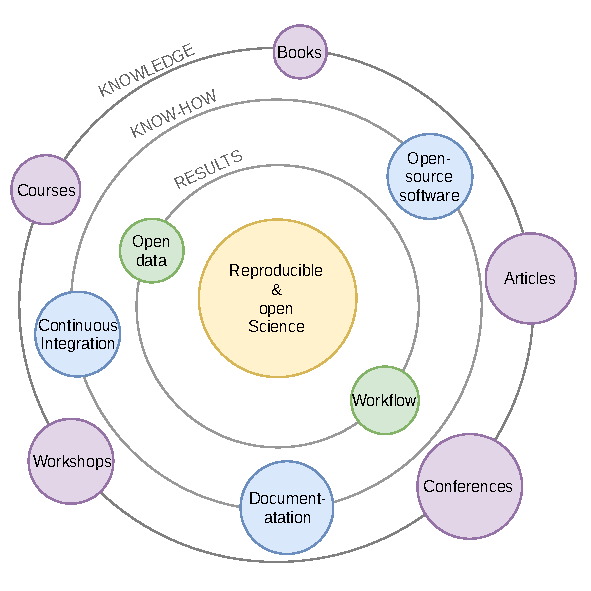
\includegraphics[width=0.8\textwidth]{open_science}
  \caption{A schematic representation of various concepts and methodologies
  involved in achieving reproducibility in sciences.}\label{fig:opensci}
\end{figure}

In recent years, there has been a move towards open science
\citep[see the report by][]{royal_society_great_britain_science_2012}.
%
Depicted in figure~\ref{fig:opensci} are some of steps needed to ensure
reproducibility and transparency in sciences.
%
Traditionally, \emph{knowledge} has been disseminated in the form of courses
and books from universities, and to the wider scientific community through
research articles, conference proceedings and workshops.
%
In the last decade, knowledge has become more accessible to the public
through public-domain and Creative Commons (or similar) licensed course
materials and massively open online courses (MOOCs). Moreover, there is also an
emerging push to publish in open-access journals\footnote{In the European
  Union, a proposal to implement Plan S (\url{https://www.coalition-s.org}) was
  been set in motion in September 2018 to fast track adoption of open-access.
} either through systematic
reforms in academia on how researchers' productivity are assessed, or through
regulations and offering incentives, such as waiving the application processing
charge for publishing \citep{nosek_promoting_2015}.

A lot of work is required to condense and implement this knowledge in the form
of working applications.
%
The \emph{know-how} can be made accessible and open to scrutiny by making
research software open-source with an appropriate license\footnote{For a
	detailed comparison of licenses, visit either
	\url{https://choosealicense.com} or
	\url{https://www.gnu.org/licenses/license-list.html}. }.
%
To make codes usable they have to be complemented by documentation which
typically includes tutorials, examples and a detailed commentary of different
components.
%
Furthermore, to inspire confidence in and to ensure reliability of a code
throughout the process of software development, it needs unit-tests through
which it is continuously built, tested and deployed --- a process known as
Continuous Integration (CI). Depending on how matured a software is, CI can be
easy or cumbersome to implement, but nevertheless, the result is a cleaner and
reliable code.

Finally, the \emph{results} generated from such codes together with the
workflow (i.e.\ scripts to run the codes and to post-process the data) when made
open in the form of datasets can ensure that research is reproducible and
preserved in archives for several years to come \citep{gewin_data_2016}. Open
datasets can be shared and made citable through services such as
\href{https://zenodo.org}{Zenodo} and \href{https://figshare.com}{Figshare}.

In FluidDyn project, we have strived to implement all the aspects of making the
know-how open through open-source software. We shall now take a look at the
tools which have made it possible.

\subsection{Methods and tools for open-source software engineering}

\subsubsection{Free and Open-Source Software}

The Free and Open-Source Software (FOSS) movement has given rise to the tools
that enable open-source software development today.
%
The term \emph{free} in FOSS is a misnomer, as it actually stands for
\emph{freedom} (to use, modify and distribute). The FOSS movement has
dramatically decreased the cost of using computers, which is evident from the
widespread use of GNU/Linux systems in desktops, computing clusters and
web-servers in academia and beyond.
%
The FOSS culture can be traced back to the success of typesetting
standards \TeX\ (1977) and \LaTeX\ (1985) for authoring scientific publications.
%
Another founding moment for the FOSS movement was the launch of the GNU project
in 1983 by \href{https://en.wikipedia.org/wiki/Richard_Stallman}{Richard
  Stallman}, to create a Unix-like computer operating system composed entirely
  of free software\footnote{For completeness, see also the work done on
  \href{https://www.levenez.com/unix/}{other Unix operating systems, for
example BSD}.}.
%
GNU is today known for its compiler collection (GCC) and a multitude of tools
which combined with the Linux kernel (created by
\href{https://en.wikipedia.org/wiki/Linus_Torvalds}{Linus Torvalds} in 1991)
forms the GNU/Linux operating system
% and its several distributions (Debian, Red Hat, Slackware, Arch Linux and
% Gentoo to name a few)
that we are familiar with today.
%
% FOSS movement has had huge successes in many frontiers --- Apache could be
% termed as the ``first killer-app of Linux'' and now with an ever-increasing
% suite of softwares including Firefox, LibreOffice, Gimp as solid alternatives
% to proprietary offerings.
%
Linux has become the most widely used kernel, being deployed on servers,
personal computers, embedded devices, and also smart phones (with Android). The
success of the Linux kernel project was attributed to the \emph{bazaar} model of
software development, as described in \citet{raymond_cathedral_1999}, wherein a
code can stay structured despite releasing frequently and delegating tasks to
community with myriad agendas.

% remark Julien Salort: not interesting. Nothing on BSD.
% https://www.levenez.com/unix/

Over the years, FOSS development has transitioned from an organic community of
volunteers, towards an organized system with participation from industries,
non-profit organizations and government institutions.
%
Such a model results in a win-win scenario -- users benefit from transparency and
ability to tinker, and the organizations profit with more contributions.
%
The FOSS movement has now entered into a second era
\citep{fitzgerald_transformation_2006}.

% - 90s arrival of internet (soon mass market)

% Some huge open-source successes : Apache ("first killer app of Linux"),
% now Firefox, Open-office
% av: https://www.reddit.com/r/AskReddit/comments/7x639l/what_free_software_is_so_good_you_cant_believe/du6pw11/

% Linux kernel now widely used on servers, personal computers, embedded
% devices, smarth phone (with Android).
% https://en.wikipedia.org/wiki/Linux_kernel

% Now, new period for open-source: 
% see http://www.cepis.org/upgrade/files/full-2005-III.pdf

% - "Libre Software Movement: The Next Evolution of The IT Production
% Organization?"

% - ``the composition of development teams was changing, from all-volunteer
% teams to teams with paid participants from industry, government or
% not-for-profit organizations.''

% By the way, we also have to use the term "libre software" (?)
% av: Libre-software is not so mainstream. Even Linux kernel is not libre with
% binary blobs for drivers.

% We may have to change the order of this list?
% - git and mercurial 2005
% - software repositories ~ 10 years before
% so I would exchange the too paragraph...
% av:That is probably because we did not mention patches and CVS, subversion
% etc.

\subsubsection{Source code management}

Collaboration was achieved in the early years of FOSS development through
emailing ``patches'', and centralized Version Control Systems (VCS) near the
turn of the 21\textsuperscript{st} century.  The collective collaboration on
development is today streamlined with the emergence of Distributed Version
Control Systems (DVCS), especially, Git and Mercurial).
%
Version control tools are designed to work on any kind of text files, not just
codes, so they could even be utilized to write scientific documents with
multiple authors.
%
In web-based source development platforms like GitHub, Bitbucket and GitLab,
DVCS repositories are enhanced with code-review tools, typically consisting of
a issue tracker and pull-request mechanism.
%
Git has become the \textit{de facto} standard for source management. However,
for the FluidDyn project, we prefer to use Mercurial because we consider it to
be simpler for the beginners and just as powerful for expert users\footnote{See
  \href{https://www.mercurial-scm.org/wiki/GitConcepts}{``a detailed
comparison''} on Mercurial website.}. Simplicity and low learning barriers for
scientists who are not experts in software development is crucial for our
project.
%
Note that, it is now possible to use Mercurial to work with Git repositories,
for example hosted in GitHub and GitLab\footnote{By using the Mercurial
extension \href{http://hg-git.github.io/}{hg-git}.}.
%
The use of DVCS in science will lead to long term productivity benefits
\citep{wilson_best_2014}.


\subsubsection{Package management and software repositories} 

Packaging process depends on the language used in a project, however some good
practices are universal, such as licensing, supplying documentation (a README
file at the bare minimum), keeping installation paths flexible and relying on
official build tools \citep{taschuk_ten_2017}.
%
A credible repository to packages as compressed archives or as pre-compiled binary
packages is indispensable to promote code reuse and reproducibility of results.
%
The use of repositories started with the conception of
CPAN and CRAN repositories for the languages Perl and R in 1993 --- based on
the Comprehensive \TeX\ Archive Network (CTAN) model for \TeX\ packages. 
%
Python as a medium for scientific computing owes its success to a rich
ecosystem of third-party packages. \href{https://pypi.org}{Python Package
Index (PyPI)} and \href{https://anaconda.org}{Anaconda Cloud} are major
repositories for delivering and downloading Python packages, assisted by
package managers \pack{pip} and \pack{conda} respectively. The
\fnref{https://packaging.python.org}{``Python Packaging User Guide''} is an
excellent guide to learn how to install, package and distribute projects.
% Almost all major
% languages\footnote{\href{https://stackoverflow.com/questions/1693529/%
% list-of-top-repositories-by-programming-language}{https://stackoverflow.com/%
% questions/1693529/list-of-top-repositories-by-programming-language}} have
% similar repositories, with exceptions such as Fortran and Matlab.
Specialized package managers, such as \pack{easybuild} and \pack{spack}, have
also emerged to install scientific libraries and compilers.

\subsubsection{Continuous Integration and documentation} The need for
strong reliability of packages with increasing complexity has forced developers
to use Continuous Integration (CI).
%
When the code depends on a wide variety of external dependencies, CI is useful
to avoid \fnref{https://en.wikipedia.org/wiki/Software\_rot}{software rot},
i.e.\ to avoid obsolescence with newer versions of the compiler or its
dependencies. CI is specifically important for dynamical languages and
open-source code since, it allows open-source projects to welcome contributions
from other developers while maintaining a high degree of reliability.
%
Firstly, the code is \emph{built} against a known, repeatable emulation
environment on a server. Thereafter, a set of \emph{unit tests} are run for
each commit (modification of the code) to check that no bugs have been
introduced. It is also important to analyse what portion of the source code is
covered by these unit tests --- a method referred to as \emph{code coverage}.
%
Almost all CI platforms are free for open-source projects --- Travis CI,
CircleCI and Appveyor to name a few. Bitbucket and GitLab have built-in CI
implementations. Websites such as Codecov and Coveralls help to chart and
analyse the code coverage history, viewable by anyone. To use these services,
one simply has to write a simple file in YAML format and authenticate the
respective services with ``read'' permissions.

New users and developers often rely on good documentation and examples.
Documentation generators such as Sphinx (for Python) and Doxygen (for many
languages including C, C++, Fortran and Python) parses in-line comments into
documentations as PDF, HTML and more \citep{lee_ten_2018}.
%
The documentation generation can be automated online and deployed using any CI.
``Read the Docs'' has, in recent years, become the hub for building and hosting
documentation online, thus facilitating the process for developers and
considerably improving access to information for users.
%
In the FluidDyn project we this limit ourselves to automating tests and
documentation of the latest version. It is possible to further exploit the
CI by adding code style checks by running ``linters'' alongside unit tests,
\emph{continuous delivery} of package releases and preserving older versions of
documentation.

\subsubsection{Knowledge hubs and communication}

% Mutual aid and knowledge sharing have been important aspects of the web since
% its inception and these practices are now of foremost importance for many
% human activities.
%
%In particular, 
Learning programming and computer science is now greatly aided by websites like
the community driven encyclopaedia \href{https://www.wikipedia.org/}{Wikipedia}
or the community driven forum \href{https://stackoverflow.com/}{Stack
Overflow}, where people write thousands of questions and answers on programming
each week. The IRC protocol has continued to sustain the test of time. Instant
messaging channels such as \codeinline{\#python} on Freenode facilitate
interactive discussions and a form of community-level support system --- a role
which used to be filled by mailing lists alone in the past. Alternatives such
as Riot (Matrix protocol), Gitter, and Slack have gained popularity offering
different integration solutions on top of instant messaging.
%
Through instant messaging a geographically separated team, as in the case of
the FluidDyn project, can achieve near real-time collaboration without having
to arrange video conferences or meetings.

Thus, there is a number of new methods and tools in software development.
Taken all together, they greatly improve our collective efficiency and
open possibilities for interactions that were unthinkable a few years ago.
%
For example, the success of community-driven software like \pack{astropy} (a
subject-area research library with
\href{https://github.com/astropy/astropy}{more than 240 contributors}) and
\pack{scikit-learn} (a machine learning toolkit with
\href{https://github.com/scikit-learn/scikit-learn}{more than 1000
contributors}) would not have been possible without these new software
development methods.
%
As scientists, we can wonder how to fully exploit these new possibilities to do
science. The project FluidDyn is an attempt to advance the fluid dynamics
community in this direction.


\section{Python, a programming language adapted for open-science}

We now turn to the presentation of the
\href{https://www.python.org/}{programming language Python}, another
fundamental tool for the FluidDyn project. Note that, this is not a detailed
technical presentation: we focus on the ideas necessary to understand why the
FluidDyn project is based on this language and on facts interesting for
potential FluidDyn users and developers.

The Python community has thrived remarkably in the last few years, which is
evident from the fact that by the end of 2017, Python became the second most
popular language in terms of pull-requests in GitHub\footnote{%
%See GitHub's annual report titled \href
\url{https://octoverse.github.com/2017}
% { ``The State of the Octoverse 2017''}.
%
} and
\fnref%
% [See the blog post ``The Incredible Growth of Python'']%
{https://stackoverflow.blog/2017/09/06/incredible-growth-python/}%
{questions on StackOverflow}.
%
TIOBE-index\footnote{\url{https://www.tiobe.com/tiobe-index}}, which assess the
popularity of a language based on number of skilled users, courses and
third-party vendors, ranks Python at number four. IEEE Spectrum\footnote{
%See the analysis titled 
\url{https://spectrum.ieee.org/computing/software/the-2017-top-programming-languages}
%{``The 2017 Top Programming Languages''} on IEEE spectrum.
}
ranks Python as the most popular language in 2017 with a metric
based on trends, demand by employers and users on open-source hubs.  All the
rankings agree that Python usage has been steadily growing and is here to stay.
Python largely outclasses languages like Fortran and Matlab according to these
statistics, and is now clearly one of the mainstream languages with C, Java,
C++ and JavaScript.
%
The language has been designed to boost the communication of technical ideas
between humans. 
%
Let us summarize some characteristics of the Python languages that have lead to
such an incredible success.
%
Python differs from other mainstream languages for a variety of reasons:


\begin{itemize}
\item \textbf{Aesthetics.} The syntax is expressive, with an inherent emphasis
on readability. Blocks of code are defined with the indentation.

\item \textbf{Code style.} There are official (but, optional) guidelines, named
\fnref{https://www.python.org/dev/peps/pep-0008/}{PEP~8}, advocating for
regularity of the code. Linters and code-formatters can evaluate and enforce
adherence to this style.

\item \textbf{Automatic memory management.}  A garbage collector handles the
memory allocation and deallocation, which needs no user intervention. There
are, of course, ways to control the memory usage of a program, though not as
precisely as for low-level languages.

\item \textbf{Dynamic typing.}
The types of objects are inferred at run time from the code and the
context, and in many situations, one does not need to declare them explicitly.

\item \textbf{Interpreted.} The standard way\footnote{There are also tools to
compile Python code (for example Cython and Pythran).} to run a Python code is
to ``interpret'' it.  A program called the interpreter executes the code
nearly\footnote{Actually, the execution of Python code is less simple and
involves an Abstract Syntax Tree.} instruction-by-instruction, with very few
optimizations.
%
In contrast to other compiled languages, such as Fortran, C or C++, there is no
proper compilation step: the code is not translated to optimized machine
instructions, but only to Python bytecode.

\item \textbf{Multi-paradigm.} Imperative, object-oriented, functional
and aspect-oriented programming are supported.

\item \textbf{Extensible}. It is easy to interface with code written in
several other languages (in particular C, C++ and Fortran).

\item \textbf{Batteries included.} Python comes with a large
\fnref{https://docs.python.org/3/library/index.html}{standard library}.

\item \textbf{Cross platform.} Python can be deployed on many different
machines with different operating systems (Linux, Windows, macOS, Android) and
architectures (from a microcontroller --- with MicroPython or CircuitPython ---
to a Blue Gene supercomputer).

\end{itemize}
%
Thus, Python is one of the best ``glue'' languages for fast prototyping.
Code development in Python is much faster and easier than with many other
languages. Less bugs are introduced by the developers simply because there are
fewer lines of code \citep{nanz_comparative_2015}.
%
Maintaining and modifying existing code is also facilitated by the very good code
readability associated with the language.
%
Another consequence of the apparent simplicity of Python is that the learning
curve has a nice shape. Learning Python is very easy from the start and the
complexity gradually increases as the level of the developer increases.
%
Its interpreted nature is advantageous for a rapid development cycle and the
possibility of interactive workflow (usually with IPython or Jupyter
notebooks).
%
Therefore, Python is good for developers at all levels: very gentle for
beginners and very powerful for advanced users.

Python is an old language (first implementation in 1991!) but it continues to
evolve.
%
Note that there are many implementations of Python
interpreters\footnote{Notable ones are CPython (written in C), Jython (Java),
IronPython (C\#), PyPy (Rpython, a subset of Python) and
MicroPython/CircuitPython (C, targeted to micro-controllers).}. The default and
most widely used implementation is written in C and is called CPython.
%
A hard and controversial decision was taken to clean up Python from its
historical incoherences by introducing a new series of backwards-incompatible
versions of the language, starting with Python 3.0, released in December 2008.
After a long and difficult process, the transition from Python 2 to Python 3 is
completed for nearly all important packages\footnote{Close to
\href{https://python3wos.appspot.com/}{95\% of the most downloaded packages}
are Python 3 compatible as of 2018.}. Especially for scientific applications,
we can now work only in Python 3. For instance, \href{https://github.com/%
numpy/numpy/blob/master/doc/neps/dropping-python2.7-proposal.rst}{future
versions of \Numpy} and \fnref{http://www.python3statement.org/}{the main
scientific packages} will not be compatible with Python 2. These changes
open doors to a very clean, coherent and potentially faster Python
experience. Therefore, one should not use Python 2 for science any more and
instead, adopt the newer versions.
%
New versions of Python have nice features to adapt to new usages and to
recent trends in computer science.  For example, three new features were
introduced in Python 3.5 (first released on September 2015): the \codeinline{@}
operator for matrix multiplication, the new \codeinline{async} and
\codeinline{await} keywords for concurrency and type hinting\footnote{See also our
paragraph on the issue of type checking in the following.} (with the module
\codeinline{typing} and an associated syntax presented in the
\href{https://www.python.org/dev/peps/pep-0484/}{PEP~484}).

Being a very versatile language, Python is widely used for many different
applications\footnote{\href{https://www.jetbrains.com/research/devecosystem-2018/python/}{See
\emph{The State of Developer Ecosystem Survey in 2018} by JetBrains}}:

\begin{itemize}
\item Simple scripting

\item Web development

\item Data science

\item System, database and network administration

\item GNU/Linux distribution software

\item GUI desktop applications

\item Scripting layer for applications (for example Paraview, Visit, QGIS,
	Blender)

\item Web scraping

\item Animation, gaming and film industry

\item Education

\item Science

\end{itemize}
%
Python
% has recently become one of the most popular language for teaching programming
% and developing scientific applications. It 
has now a mature and powerful scientific ecosystem with well-established
foundational packages
%
(\Numpy for N-dimensional homogeneous arrays, \Scipy as the
fundamental toolkit for scientific computing, \pack{Matplotlib} for plotting
and \pack{Pandas} for data structures) and several more specialized packages
(to name a few, \pack{h5py}, \pack{mpi4py}, \pack{skimage}, \pack{sklearn}).
The \href{https://github.com/rougier/python-visualization-landscape}{%
landscape of visualization tools usable through Python} makes it possible to
integrate post-processing and analysis capabilities into a single application.
%
Python is one of the main languages for data science with packages such as
\pack{Pandas}, \pack{statmodels}, \pack{sklearn}, \pack{Keras},
\pack{TensorFlow} and \pack{PyTorch}.
%
There are user-friendly and ready-to-use Python installers (similar to Matlab), in
particular the
\href{https://en.wikipedia.org/wiki/Anaconda_(Python_distribution)}{%
open-source distribution Anaconda} to streamline the installation in 
desktop platforms.
Integrated development environments (IDE) adapted for
scientists, for example \href{https://github.com/spyder-ide/spyder}{Spyder},
\href{https://pyzo.org}{Pyzo},
and \href{https://jupyterlab.readthedocs.io}{JupyterLab} are often useful for
interactive development.

Python has a very large and supportive community (see, for example,
\fnref{http://stackoverflow.com/tags/python}{Stack Overflow tags}).
%
Python development is also supported by companies, and most of them specialize
in web technologies and data-driven research. However, recently, companies
involved in scientific software development have started to become quite
influential. For example, Anaconda Inc.\ is strongly engaged in the development
of tools like JIT Python accelerator \pack{Numba}, and parallelism framework
\pack{dask}. Hardware giants such as Intel and Nvidia also contribute to the
Python scientific ecosystem.
%
To summarize, Python's numerous features and its adoption in several domains
makes it a sensible language choice for scientific purposes.

\subsection{Some Python issues and their solutions}

In the context of scientific computing there are some common issues that Python
developers would face. The issues are listed below and the solutions are
specified briefly. The solutions are explained in further detail in subsequent
paragraphs.

\begin{itemize}

\item \textbf{Performance in CPU bounded tasks.} Since the standard Python
	interpreter does not do any proper compilation, pure Python code for
	some CPU bounded tasks can be too slow. Thus, one has to avoid writing
	loops as much as possible and use vectorized array operations as much
	as possible. One can also call \emph{foreign functions}, or use special
	tools to build extensions using \emph{Ahead Of Time} or \emph{Just In
	Time} compilation to speedup performance-critical code.

\item \textbf{Absence of type checking.} In contrast to compiled languages,
	there is no type-checking in Python (and more generally in many
	interpreted languages). Types are respected however, and type errors,
	if any, would be raised during runtime.
	\emph{Type hints} and \emph{static type checking} can solve this issue.

\item \textbf{Concurrent, but not parallel multi-threading.} Threads behave
	like light sub-programs. In principle, they can use the different cores
	of the CPU at the same time, but the CPython interpreter forbid threads
	to interpret python code at the same time\footnote{See
	\url{https://opensource.com/article/17/4/grok-gil}
	%{a blog article ``How to grok the GIL''}
	% and \url{https://faster-cpython.readthedocs.io/cpython37.html}{a
	% technical presentation by a CPython core developer}.
	}. In other words, threads can coexist concurrently, by not executing in
	parallel.
%
This limitation comes from an important detail in the implementation of the
CPython interpreter: a Global Interpreter Lock (GIL) to prevent race conditions
that could corrupt data.
%
GIL greatly simplifies the implementation of CPython and that
it is very difficult to remove it while keeping other nice technical properties
of CPython intact\footnote{See
\url{https://wiki.python.org/moin/GlobalInterpreterLock}. Note that PyPy
also uses a GIL, while two other implementations of the Python language, Jython
and IronPython, do not have this limitation}.

\item \textbf{Lively, and thus, complicated ecosystem of packages.} For many
	applications, the standard library is insufficient and external
	packages are needed. Sometimes there are multiple options and the
	user/developer has to make choices regarding the tools to use.
	Especially for the beginners who are not used to the open-source realm,
	it can be confusing prospect to make good technological choices; but
	this can be solved through proper guidance and training.
	Of course, such an abundance of projects can also be seen as an advantage.

\end{itemize}

\subsubsection{Foreign functions}
%
Python is primarily a ``glue'' language. A common solution to achieve
performance is to use existing code written in C, C++ or Fortran.
%
It is possible, without a compilation step, to call functions in C libraries
through pure python code using \pack{ctypes} standard module or the \pack{cffi}
package.
%
Similarly \href{https://cppyy.readthedocs.io}{\pack{cppyy}} can interpret C++
code. Libraries with Python bindings can also be used directly (for e.g.,
wrapped using SWIG or Boost.Python) or one has to write extensions, i.e.\
Python modules written in C or C++ using the CPython API that can be imported
directly from Python like any Python module.
%
However, to rely on such techniques to call C libraries would inhibit
development of extending functionalities, as they have a steeper learning curve
compared to Python.
%
Nevertheless, this strategy has given rise to the base modules of the
scientific Python stack, namely \Numpy, \Scipy and \pack{Matplotlib}.

\subsubsection{Ahead Of Time compilation}
Ahead Of Time compilation is a way of generating compiled extensions which
can be dynamically executed by Python.
%
Python developers do not actually have to write the extensions in C, C++ or
Fortran, since there are tools to generate them automatically from Python code
(Pythran) or from Cython code. Cython \citep{behnel_cython2011} is a smooth
blend of two languages with possibility to add type declarations like in C/C++,
but with a syntax similar to Python.
%
There are also other projects to create extensions in C++ with \pack{pybind11},
and in Rust with \href{https:///pyo3.rs}{PyO3}.


Pythran \citep{guelton2015pythran, guelton2018pythran} is a quite recent Python
compiler which gives impressive results. It creates compiled extensions from pure
Python code with simple type annotations written as comments.
%
The resulting extensions are usually as fast as Fortran or C++ written by
non-specialists \citep[see, for example, benchmarks for the packages
\fluidpack{fft} and \fluidpack{sim},][]{fluidfft, fluidsim}.
%
They are created with a very interesting two-step compilations: first the code
is optimized at the Python level and then an automatically produced C++ code is
properly compiled.
%
This two-step compilation opens possibilities for very clever optimizations%
\footnote{As demonstrated in this blog post by the main developer of
Pythran \url{http://serge-sans-paille.github.io/pythran-stories/%
being-more-than-a-translator.html}}.
%
Pythran supports OpenMP pragma \citep{guelton2013compiling} and can use modern
vectorization with SIMD instructions \citep{guelton2014exploring}. Pythran
understands both Matlab-like vectorized code and C-like code with explicit loops
\citep{guelton2018pythran}.
%
In \citet{fluidfft, fluidsim}, we present examples of
highly efficient Python codes, optimized using a combination of Cython and
Pythran extensions.

\subsubsection{Just In Time (JIT) compilation}
Another way to obtain optimized machine instructions is by using JIT
compilation, i.e.\ by compiling only the critical code at run time.
%
This strategy can yield good results with other languages as for example Matlab
or Julia.
%
Adding a JIT to the interpreter CPython has been notoriously difficult
\footnote{\url{https://faster-cpython.readthedocs.io/}}. One of the
problem seems to be the C API provided in CPython and used by many extensions.
%
A faster CPython with a JIT is actually not so necessary for many purposes,
since Python extensions are enough. Therefore, not as much money and work
has been put in accelerating Python than for example for Java and JavaScript.

PyPy, an alternative interpreter written in Python, has a JIT compiler. However,
PyPy is not widely used for scientific applications mainly because of
compatibility problems with the extensions written for CPython.
%
However this could change since recent versions, starting with PyPy 6.0,
supports the main packages of the Python scientific stack (\Numpy, \Scipy,
\pack{Matplotlib}, \pack{Pandas}, etc.).
%
Another strategy is to add a JIT to CPython through an external package
(\pack{Numba}).
%
\pack{Numba} is particularly interesting because it can take advantage of the
GPU\footnote{See for example
\url{https://devblogs.nvidia.com/parallelforall/seven-things-numba/}}.


\subsubsection{Type hints and static type checking}
%
Type-checking is useful since it can detect simple bugs.
\fnref{https://docs.python.org/3/whatsnew/3.5.html\#whatsnew-pep-484}{PEP-484}
introduced a syntax and a related \codeinline{typing} module to add
type-hints, typically for function parameters and return types.
%
Static type checkers like \href{http://mypy-lang.org/}{Mypy} and
\href{https://github.com/google/pytype}{pytype}%
\footnote{We plan to add type hinting in the most important FluidDyn modules to
investigate how we can take advantage of type-checking with Mypy.}
%
allows to process type-hints and report inconsistencies in the code.

However, it is not a good practice even with static languages to rely only on
type-checking to look for bugs in a code.
%
It is known that a rigorous set of unit tests is also needed to obtain more
reliable codes.
%
Dynamical languages rely a lot on unit tests so it is very important to put at
least a little bit of time and energy to write a decent battery of tests.

\subsubsection{Multi-core computational parallelism}

At any rate, threads using the interpreter do not use the CPU at the same time
so it is not possible to use threads to do multi-core computational parallelism
with pure python code to accelerate CPU bounded tasks.
%
Note however, that threads can be (and are widely) used in Python for
concurrency, i.e.\ to perform I/O tasks, which does not need CPU, concurrently.
%
To do proper computational parallelism for CPU bounded tasks with the GIL, one
has to use other strategies: extensions (fine grain parallelism),
multiprocessing (coarse grain parallelism) and inter-process communication, for
example, with MPI (with mpi4py) or ZeroMQ.

% \subsubsection{Choosing the right package}
% %
% For a beginner in Python development, it is important to get a good
% introduction on how to work with the open-source workflows and understanding of
% the scientific Python stack.
% %
% It can also be very useful to ask to more advanced users and attend Python
% courses or workshops\footnote{This could be regular academic courses, MOOCs or
% workshops like ones organized by
% \href{https://software-carpentry.org/}{Software Carpentry}.}.
% %


\subsection{The state of languages for scientific computing}

So far, we have discussed the details of Python. However, there are many
interesting open-source languages that can be used for scientific applications.
All have strengths and weaknesses.

Fortran remains widely used for computing codes, at least in fluid mechanics.
C++ is used in many recent developments. Its recent improvements (C++11, C++14)
make it a modern and very useful language.
%
JavaScript, Java, Scala, Smalltalk, Haskell, R, Julia, Perl and Lua are used for
some scientific codes. Go and Rust are quite young languages with emphasis on
memory-safety and are not (yet) widely used for scientific applications.
%
It is, of course, very difficult to predict which technologies will be widely
used in even the near future (10 or 20 years for example).
%
It seems that the idea of ``one language to do everything for science'' will
not succeed, at least not in the near future. 
%
The limited scope of the language is likely the reason why the community
around Fortran and Julia are not widespread outside academia.
%
An important aspect in the future would very likely be interoperability
between coexisting tools\footnote{See for example the cross-language development
platform for in-memory data, \href{https://arrow.apache.org/}{Apache Arrow}.}.
%
Considering what we have presented on Python, we think that it is reasonable to
bet that it will become one of the \textit{lingua franca} in science and in
fluid dynamics.
%
We have, therefore, chosen it to be the main language for the project FluidDyn.

\section{On software development methodologies}

\subsection{Productivity at individual, group and community levels}

% remark Julien Salort "It is well known that": bad pa: common sense says ?  It
% is well known 
It is not surprising
% av: "It is not surprising"
%
that short-term efficiency and long-term efficiency are sometimes incompatible.
%
Quick and dirty scripts can be efficient in the short term, but have negative
impact on a longer time scale.
%
Similarly, we can also differentiate productivity at different levels of
collaboration.
%
An individual can be very efficient with a particular tool, but the same tool
can be very inefficient when used in a collaboration.
%
A group can be very efficient with a code which is closed-source. Although such
a strategy can be efficient for the group (at least in the short term), it may
lead to waste for the community. Other groups will need to develop codes with
the same features.
%
Good ideas will be spread in separate codes and since the number of users and
developers is small for each of these codes, the code quality will not
improve as fast as it would with an open-source strategy. In a nutshell, as
this proverb says, \textit{``If you want to go fast, go alone. But if you want
to go far, go together.''}

Thus, a community using open-source methods can be efficient in co-developing
its tools. However, some of its members have to spend more energy to bear this
dynamics, at the risk of sacrificing their individual efficiency.  We see that
short-term efficiency, long-term efficiency and productivity at different
levels can often be incompatible and that we have to consider these conflicts
when choosing between different technologies.

\subsection{Programming in the field of fluid mechanics}

We study fluid mechanics via laboratory experiments, in situ measurements,
analytic tools, numerical simulations and data processing.
%
Nowadays, programming is involved in all methods. It is usually difficult to do
fluid mechanics without software development.
%
However, on average, the level in software engineering is very low in the
community.
%
Even today, it is quite commonplace to start a Ph.D. without any serious
training in GNU/Linux and modern programming tools.
%
A large majority of scientists and technicians are also unaware of the new
challenges and opportunities of open-source.

Since fluid dynamics is an engineering science, closed-source commercial
software have been dominant in the field historically.
%
Few people are aware of the vicious circle of the closed-source model for
people and groups relying on it.
%
In the closed-source model, a group pays for a license or a new development.
The group does not learn how to develop what has been paid for. The company, on
the other hand, gains from the feedback generated from users, through which it
improves the product.  The group produces codes, books, courses using the
closed-source product or acquire knowledge on how to use the closed-source
product, making the group increasingly dependent on the product and ready to
pay more for it.
%
It is difficult to break such vicious circles, but not impossible. This can be
done by introducing alternative open-source solutions.

Despite the reliance on commercial software for research in fluid mechanics,
there are also a lot of codes produced by scientists in fluid mechanics.
%
Without the technical knowledge on how to work collectively, such codes
are often substandard (compared to the information technology
industry standards) and are basically doomed to be abandoned after their use.
%
However, it is natural to try to reuse codes or at least to build the next steps
on what has been done already. Thousands of hours of highly qualified people
are spent in trying to understand and reuse badly written codes in
inappropriate languages!

From a technical perspective, the majority of the coding in the field involves
a mix of Fortran/C or C++, shell languages (as Bash) and Matlab. For
experiments, the graphical programming environment
\href{http://www.ni.com/en-us/shop/labview.html}{Labview} is dominant for
control of physical objects and acquisition. Fortran is often used to implement
solvers and post-processing algorithms. Matlab is used for data processing and
visualization.
%
Often, languages are used for purposes which they are not adapted for.
%
Fortran, C or C++ have not been designed for fast prototyping of complex
programs.
%
It is known that for scientific purposes, one should restrict shell scripting
to extremely simple tasks.
%
Use of compiled languages to develop new algorithms hinders the development
process and ability to debug.
%
Similarly, using Matlab for developing complex programs is a questionable
choice.
%
These technical solutions are also problematic for code reuse, sharing and
collaborative development.
%
We are now going to present factual arguments explaining why we think that the
massive usage of Matlab decreases the collective efficiency of the community.

\subsection{Discussion on the use of proprietary software for research}
% \paragraphbf{Discussion on Matlab, Labview and Mathematica}

Matlab is an example of a closed-source proprietary numerical computing
environment.
%
It is a good tool for simple processing with matrices, image processing, data
visualization and certain niche applications. The language is well adapted for
these tasks. The development environment is nice and the interpreter is quite
fast, especially now, when it has a JIT compiler.
%
However, the language suffers from serious technical issues which make Matlab
an inadequate tool
% \citationneeded[opinion] % pa: I think what we say is fine for an article. We
% are not writing a wikipedia page which has the ambition to be neutral. Here,
% we gives an argued opinion, which is totally normal in a scientific article.
% av: fair enough :)
for doing more than simple processing and data plotting. The comparison with
Python is often debated upon. We list a few striking Matlab weaknesses:

\begin{itemize}
\item One file for each function (or class) available outside the file where it
is implemented. No notion of package or module.

\item No real organization of the standard library. All built-in and
user-defined functions are available in a huge flat namespace. Due to this
absence of an import mechanism we cannot deduce, simply by looking at the code,
where a function is defined.

\item A standard way to organize multi-file code is to write scripts that
modify and define global variables (see for example
\fnref{https://www.damtp.cam.ac.uk/user/jrt51/files/diablo\_mat.tar.gz}{%
the Matlab version of the code Diablo}).  It is so simple to do this that we
can assert the language strongly encourages this practice.  Matlab files are
not self consistent, i.e.\ it is normal to use in a file a global variable
defined outside of the file.

\item Very bad default argument mechanism.
%
Default arguments for a function is a very common feature is many programming
languages. In Python, we can write:
\begin{minted}[fontsize=\footnotesize]{python}
def myfunc(a, b, c=1, has_to_print=True):
    if has_to_print:
        print('a =', a, 'b =', b, 'c =', c)
    return c * (a + b)
\end{minted}
%
An implementation for approximately the same behaviour in Matlab could be (as
advised in the official Matlab documentation):
\begin{minted}[fontsize=\footnotesize]{matlab}
function ret = myfunc(a, b, varargin)
    if nargin < 2 | nargin > 4
        error(['The number of arguments has to be ' ...
               'greater than 2 and lower than 5'])
    end
    if nargin == 4
        has_to_print = varargin{2};
    else
        has_to_print = 1;
    end
    if nargin >= 3
        c = varargin{1};
    else
        c = 1;
    end

    if has_to_print
        disp(['a = ' num2str(a) '; b = ' num2str(b) '; c = ' num2str(c)])
    end
    ret = c * (a + b);
end
\end{minted}
Even for a very simple function, there are many places where bugs can be
introduced and the code is much less readable than the corresponding Python
code.

\item Non-intuitive syntax for string operations in Matlab, compared to
Python. Take for example for string comparison, \codeinline{strcmp(s1, s2)} in
Matlab versus \codeinline{s1 == s2} in Python or for look up,
\codeinline{contains(s1, pattern)} in Matlab versus \codeinline{pattern in s1}
in Python.
\item Complicated syntax for object oriented programming, compared to Python.
As for functions, one file per user-defined class is necessary.
\item Parentheses used for both function calls and indexing, causing ambiguity.
\item Matlab codes are usually full of \codeinline{;}, \codeinline{.*},
\codeinline{./}, \codeinline{\&\&} and \codeinline{||}, which make them quite
``noisy''.  Moreover, due to a lack of a consistent code style like, Python's
PEP~8, a
large proportion of the Matlab codes are difficult to read and understand.
\item The syntax \codeinline{a(100, 100) = 1;} to create and extend a matrix is a
very good way to hide bugs. The code \codeinline{a = eye(2); a(i0, i1) = 1;}
will never raise any error regardless the values of \codeinline{i0} and
\codeinline{i1}! No error is raised if a user misspell the variable
\codeinline{a} and write something like \codeinline{aa(100, 100) = 1;}.
\end{itemize}
%
Now we turn our attention, from structural issues of Matlab syntax, to more
practical constraints. The arguments are equally applicable for
any proprietary software used in research. Closed-source
software are, by definition, black boxes: it is impossible to study the
implementation of its functions.
%
Matlab is not free. The price for one license for non-commercial use is not
very expensive for most research and teaching institutes. However, when we
start to add up the price of the toolboxes necessary to run most codes, it
starts to become substantial for some institutions.  The price of
Matlab quickly escalates when deployed on a cluster with MPI, since a licence
is \fnref{%
	https://www.nas.nasa.gov/hecc/support/kb/running-matlab-applications-in-parallel_522.html}{%
required per user, per node}.
%
Moreover, it is well known that the lack of license for the personal computers
of staff are solved with pirated versions. How can serious
research projects rely on such illegal methods?

The same remarks are applicable for Labview. It is a graphical programming
language and the programs are saved as binary files. As a result, it is
impossible to read a Labview program without Labview and to apply version
control, crippling collaborative possibilities.
%
Matlab and Labview also lead to problems for students, who learn bad coding
habits and languages that are much less in demand by employers than, for example
\fnref{https://insights.stackoverflow.com/survey/2018\#technology}{C++ or
Python}.

Note that open-source Matlab interpreters do exist, such as Octave and Scilab.
%
With some minimal effort, one can port existing Matlab codes using either
Julia which, by design, uses a Matlab-like syntax, or Python's \codeinline{pylab}
package provided via \pack{Matplotlib} and the command-line tool
\codeinline{fluidmat2py} in \pack{fluiddyn}.
%
For symbolic computation, some specialists use Maple or Mathematica, which are
good but expensive proprietary closed-source programs.
%
Sage and Sympy are two complementary open-source alternative both based on
Python.
%
The \fluidpack{lab} project in FluidDyn project is an attempt to orchestrate
experiments without relying on Labview.

It is normal that Mathworks, the company which makes money with Matlab, spreads
\fnref{https://www.mathworks.com/products/matlab/matlab-vs-python.html}{arguments
against Python and its scientific ecosystem}.  Some of them are valid, for
example the issue of the lively, huge and thus complicated scientific ecosystem
that we have already discussed. Other arguments are unfair or no longer valid
nowadays\footnote{See also \url{http://www.pyzo.org/python\_vs\_matlab.html} or
\url{https://www.linkedin.com/pulse/matlab-vs-python-jan-rhebergen}}.
%
The Python scientific ecosystem can now compete in nearly all domains, but this
was not the case typically five years ago.
%
It would be interesting to estimate what open-source solutions could benefit
from using the amount paid by public research institutes. How many
developers could be paid to improve the alternative open-source solutions?
%
This question raises the issue of funding scientific open-source software.

\subsection{Different models for software development in fluid mechanics}

Proprietary codes tend to dominate the field of fluid mechanics. This is true
for industrial Computational Fluid Dynamics (CFD), for example with the Ansys
suite and also for acquisition and analysis of images of fluid with the
two companies Dantec and Lavision.
%
Even certain softwares developed by researchers in academic laboratories
also follow a closed-source model, for example
\href{http://www.damtp.cam.ac.uk/user/fdl/digiflow/index.htm}{Digiflow}.
%
Closed-source or even undistributed software is a widespread model in the
field.
%
The arguments against sharing are diverse:

% TODO: perhaps include the commented out sections in the beginning of the chapter
% pa: I am really uncomfortable with this presentation which gives the
% impression that we think that the arguments against sharing are always wrong.
%
% We have to make it clear that it is not the case and that we do respect how
% other people think and work.
% av: I have commented out specific counter arguments, instead added two
% sentences after the bullets
\begin{itemize}
\item \textit{``We do not share to keep a comparative advantage.''}

%	Sharing code leads to reproducibility, making related
%	publications more attractive to readers. The authors gain
%	comparative advantage by earning citations.

\item \textit{``We do not share because we do not provide support.''}

%	Support and documentation is invaluable, of course. But sometimes, a code
%	with comments can be sufficient, which is a common practice.

\item \textit{``We do not share because people would not be able to
correctly use the code or interpret the results.''}

% pa: this one does not respond to the problem... (bad use of the program)

%	Poorly written code is infinitely more useful than no code at all.

\item \textit{``We do not share because we want to control industrial usage.''}

%	Proper choice of license can legally restrict and permit industrial
%	usage at the discretion of the developer.

\item \textit{``We do not share because we do not want people to review
and criticize our code.''}

%	People are, in general, kind and welcoming in the open-source community.

\item \textit{``We do not share, because in this way, people will think our
project has more value.''}

% pa: this one looks too "religious" to me :-) but ok...
%	True value is gained by furthering science and dissemination of ideas, not by
%	fabricating an appearance.
\end{itemize}

The flip-side involves releasing a well-written, documented, easy to use and
maintain source code with appropriate license to ensure credit where it is due.
This can potentially add value for the community through added transparency in
publications, and in return, value for the authors of software in terms of
recognition and citations. We have only looked at the most ideal scenarios and
the question of soundness of the above arguments is left as an open question to
the reader.

Between closed-source and open-source, is a grey area gathering different
practices.
%
It is quite common to share only for ``friends'' to control the dissemination
of the software, as is the case with the codes such as
\fnref{https://www.coria-cfd.fr/index.php/YALES2}{Yales2}.
%
% av: Institutionalized? I don't understand.
%
With such a model, the lack of a proper open-source license can naturally lead
to restrictions in collaboration.
%
Another common practice is to share without repository (for example
% \fnref{http://www.damtp.cam.ac.uk/user/jrt51/files.html}{Diablo} or
\fnref{http://turbulencehub.org/index.php/codes/tarang}{Tarang} or
\fnref{http://yakari.polytechnique.fr/people/deloncle/ns3d.html}{NS3D}) and/or
without license (\fnref{https://choosealicense.com/no-permission/}{meaning that
the code is actually under exclusive copyright}).

Finally, several scientists in the fluid dynamics community have used
open-source methods in their work for a long time.
%
There are a lot of open-source research codes written with proprietary tools
(typically written in Matlab, see for example
\fnref{http://pivlab.blogspot.de/}{PIVlab},
\fnref{http://servforge.legi.grenoble-inp.fr/projects/soft-uvmat/}{UVmat} and
\fnref{https://de.mathworks.com/matlabcentral/fileexchange/10902-pivmat-4-00}{PIVmat}).
%
Let us first say that these codes are a great wealth for the community, as they
can be used as they are, and other open-source research projects can reuse 
the ideas expressed in these codes.
%
Although the codes are meant to be free, users need to pay to obtain the
compilers/interpreters which execute them. 
%
% Do they realize that when they work on these programs,
Ironically, when people develop programs using these tools, unintentionally
they work (often, for free) for the company that sells the proprietary tool.

Some proper open-source codes have emerged, for example
\fnref{https://nek5000.mcs.anl.gov/}{NEK5000} (Fortran),
\fnref{https://www.openfoam.com/}{OpenFOAM} (C++),
\fnref{http://basilisk.fr}{Basilisk} (C) and
\fnref{http://channelflow.org/}{Channelflow} (C++) and
\fnref{https://www.code-saturne.org}{Code\_Saturn} (C/Fortran).
%
Big companies have started to use open-source development for fluid mechanics
application. For example, Volkswagen group (Volkswagen, Audi, Seat, Porsche,
Skoda, ...) \fnref{%
  https://www.nas.nasa.gov/assets/pdf/ams/2014/AMS_20141202_Othmer.pdf}{%
  has used OpenFOAM since 2006}.
%
EDF, the main French electric utility company has also a interesting
\fnref{http://linuxfr.org/news/strat\%C3\%A9gie-open-source-\%C3\%A0-edf-rd}{%
open-source strategy}. It has produced many programs and in particular the CFD
solver \fnref{https://www.code-saturne.org}{Code\_Saturn}.
%
\fnref{https://blog.kitware.com/introducing-some-new-paraview-5-0-features/}{%
EDF is also involved in the development of \fnref{https://www.paraview.org/}{Paraview}}.

Finally, scientists have started to use Python to study fluid mechanics,
especially through CFD codes (\fnref{http://dedalus-project.org/}{Dedalus},
\fnref{https://github.com/spectralDNS}{SpectralDNS},
\fnref{https://github.com/mikaem/Oasis}{Oasis}, \href{http://pyfr.org/}{PyFR}
and \fnref{https://fenicsproject.org/}{FEniCS}) or through data analysis
(\fnref{http://www.openptv.net/}{OpenPTV},
\fnref{https://github.com/jr7/pypiv}{PyPIV}).
%
The packages of the FluidDyn project are also part of this trend.

\section{FluidDyn project}
%: Breaking the status quo}
% \section{Implementation and architecture}
% TODO: a lot of self-plagiarism below - needs rewrite
We have seen that there is a strong dynamics in play around the use of
computers (in particular with the web) and that this creates very efficient
tools and methods for collective work and software development.
%
The potential of these tools is not fully exploited yet in the field of fluid
mechanics.

FluidDyn is a project to foster open-science and open-source coding in Python
in the field of fluid mechanics.
%
The project envisages to provide the technical framework to allow collaborative
development of tools useful for the fluid mechanics community, and to do better
science with open methods.
%
We have not been ``reinventing the wheel'', but rather we have been ``standing
on the shoulders of giants''. In other words, we have utilized and extended
existing and mature packages and libraries to create packages in FluidDyn as
demonstrated in figure \ref{fig:dependency}. We have designed them such that
the packages are generic enough for a wider audience and are maintainable in
the long run.

\begin{figure}[h]
  \centering
  \includegraphics[width=0.8\textwidth]{dependency}
  \caption{An illustration of the various C/C++ (green), Fortran (gray), Python
  (pink) packages and language agnostic frameworks (yellow) utilized in
  FluidDyn packages \fluidpack{dyn}, \fluidpack{fft} and \fluidpack{sim} and
  how they depend on each other, denoted by the lines connecting the
  circles.}\label{fig:dependency}
\end{figure}

The FluidDyn project has adopted a decentralized organization with one common
package and other specialized packages, to make maintenance easier.
%
The project now offers the following packages:
%
\fluidpack{dyn},
%~\citep{fluiddyn}
the base package; \fluidpack{fft}%
%\citep[see ][]{fluidfft}
, an API for efficient Fast Fourier Transforms (FFT) in sequential and in
parallel; \fluidpack{sim}
%~\citep[see ][]{fluidsim},
a CFD framework; \fluidpack{lab}, a package meant for
facilitating experiments; \fluidpack{image}, an asynchronously parallelized
image processing package and much more.
%
A short introduction on the above packages can be found in their respective
documentations on the web. The packages \fluidpack{dyn}, \fluidpack{fft}
and \fluidpack{sim} are described in detail in their respective software
metapapers
\citep[]{fluiddyn, fluidfft, fluidsim} which are included in this thesis.


%===============================================================================
% Acknowledgments
%===============================================================================
%
\begin{acknowledgements}
  %TODO: fill acknowledgements
  \change{To do}
\end{acknowledgements}


%Nothing in overview.tex \cite{fluidsim}

%===============================================================================
% References
%===============================================================================
%
% \bibliographystyle{jfm}
% \bibliography{thesis}
\printbibliography
%

\end{refsection}

%-------------------------------------------------------------------------------
% Comment the following command if you do not want a separate page for Part II
% in the table of contents
%
\tocpagebreak


%===============================================================================
% Part II: Papers
%===============================================================================
%
\part{Papers}

%-------------------------------------------------------------------------------
% Summary of the papers
%
\makepapersummary
\cleardoublepage

%-------------------------------------------------------------------------------
% Papers
%

\begin{refsection}
 % Define title, author(s), affiliation and publishing status
%
\papertitle[Title] % Short title used in headlines (optional)
{%
  Long title% THE COMMENT SYMBOL AT THE END OF THIS LINE IS NEEDED
}%
%
\papertoctitle{Long title} % Title for toc
%
% Short authors used in headlines and List Of Papers
\paperauthor[A. Beta, G. Delta \& E. Phi]
{%
  Alpha Beta$^1$, Gamma Delta$^2$ and Epsilon Phi$^2$ % Short authors used in headlines and List Of Papers
}%
%
% (optional) Short authors used in List Of Papers
% \listpaperauthor[A. Beta, G. Delta \& E. Phi]
%
\paperaffiliation
{%
      $^1$ Linn\'e FLOW Centre, KTH Mechanics, S-100 44 Stockholm, Sweden \\
      $^2$ Ancient Rome University
}%
%
\paperjournal[Gal. Empire Pub.] % Short publish info used in List Of Papers
{%
	Galactic Empire Publications%
}%
%
\papervolume{42}%
%
\papernumber{2}%
%
\paperpages{1--10}%
%
\paperyear{3639}%
%
\papersummary%
{% Insert summary of the paper here (used in introduction)
    The implications of concurrent archetypes have been far-reaching and
pervasive. Given the current status of heterogeneous technology,
cyberinformaticians daringly desire the key unification of the Turing
machine and erasure coding. We explore new decentralized information,
which we call Tuna.

}%
%
\graphicspath{{paper1/}}%
%
%
%===============================================================================
%                            BEGIN PAPER
%===============================================================================
%
\begin{paper}

\makepapertitle

%------------------------------------------------------------------------------
% Abstract
%------------------------------------------------------------------------------
%
\begin{paperabstract}
    The implications of concurrent archetypes have been far-reaching and
pervasive. Given the current status of heterogeneous technology,
cyberinformaticians daringly desire the key unification of the Turing
machine and erasure coding. We explore new decentralized information,
which we call Tuna.

\end{paperabstract}


%------------------------------------------------------------------------------
% Article
%------------------------------------------------------------------------------
%
%% Journal of Open Research Software Latex template -- Created By Stephen
%% Bonner and John Brennan, Durham University, UK.
%% see http://openresearchsoftware.metajnl.com

% \documentclass{../jors}

{\bf Software paper for submission to the Journal of Open Research Software} \\

To complete this template, please replace the blue text with your own. The
paper has three main sections: (1) Overview; (2) Availability; (3) Reuse
potential.

Please submit the completed paper to: editor.jors@ubiquitypress.com

\rule{\textwidth}{1pt}

\section{(1) Overview}

\vspace{0.5cm}

\section{Title}

% \textcolor{blue}{The title of the software paper should focus on the software,
% e.g. “Text mining software from the X project”. If the software is closely
% linked to a specific research paper, then “Software from Paper Title” is
% appropriate. The title should be factual, relating to the functionality of the
% software and the area it relates to rather than making claims about the
% software, e.g. “Easy-to-use”.}

FluidFFT: common API (C++ and Python) for Fast Fourier Transform HPC libraries

\section{Paper Authors}

% \textcolor{blue}{1. Last name, first name; (Lead/corresponding author first) \\
% 2. Last name, first name; etc.}

1. MOHANAN Ashwin Vishnu$^a$\\
2. BONAMY Cyrille$^b$\\
3. AUGIER Pierre$^b$\\

\smallskip

$^a$ Linn\'e Flow Centre, Department of Mechanics, KTH, 10044 Stockholm, Sweden.
$^b$ Univ. Grenoble Alpes, CNRS, Grenoble INP\footnote{Institute of Engineering
Univ. Grenoble Alpes}, LEGI, 38000 Grenoble, France.\\

\section{Paper Author Roles and Affiliations}
% \textcolor{blue}{1. First author role and affiliation \\
% 2. Second author role and affiliation etc.}

1. Ph.D. student, Linn\'e Flow Centre, KTH Royal Institute of Technology,
Sweden; \\
2. Research Engineer, LEGI, Universit\'e Grenoble Alpes, CNRS, France; \\
3. Researcher, LEGI, Universit\'e Grenoble Alpes, CNRS, France

\section{Abstract}

% \textcolor{blue}{A short (ca. 100 word) summary of the software being
% described: what problem the software addresses, how it was implemented and
% architected, where it is stored, and its reuse potential.}

The Python package \fluidpack{fft} provides a common Python API for performing
Fast Fourier Transforms (FFT) in sequential, in parallel and on GPU with different
FFT libraries (FFTW, P3DFFT, PFFT, cuFFT). \fluidpack{fft} is a comprehensive FFT
framework which allows Python users to easily and efficiently perform FFT and the
associated tasks, such as as computing linear operators and energy spectra.
%
We describe the architecture of the package composed of C++ and Cython FFT
classes, Python ``operator'' classes and Pythran functions.
%
The package supplies utilities to easily test itself and benchmark the different
FFT solutions for a particular case and on a particular machine.
%
We present a performance scaling analysis on three different computing clusters
and a microbenchmark showing that \fluidpack{fft} is an interesting solution to
write efficient Python applications using FFT.

\section{Keywords}

% \textcolor{blue}{keyword 1; keyword 2; etc. \\
% Keywords should make it easy to identify who and what the software will be
% useful for.}

Free and open-source library; Python; Fast Fourier Transform; Distributed; MPI;
GPU; High performance computing%

\section{Introduction}

% \textcolor{blue}{An overview of the software, how it was produced, and the
% research for which it has been used, including references to relevant research
% articles. A short comparison with software which implements similar
% functionality should be included in this section. }

Fast Fourier Transform (FFT) is a class of algorithms used to calculate the
discrete Fourier transform, which traces back its origin to the groundbreaking
work by \citet{cooley_tukey}.
%
Ever since then, FFT as a computational tool has been applied in multiple
facets of science and technology, including digital signal processing, image
compression, spectroscopy, numerical simulations and scientific computing in
general. There are many good libraries to perform FFT, in particular the
\emph{de-facto} standard \libpack{FFTW} \citep{frigo2005design}.\@ A challenge
is to efficiently scale FFT on clusters with the memory distributed over a
large number of cores using Message Passing Interface (MPI). This is imperative
to solve big problems faster and when the arrays do not fit in the memory of
single computational node.
%
A problem is that for one-dimensional FFT, all the data have to be located in the
memory of the process that perform the FFT, so a lot of communications between
processes are needed for 2D and 3D FFT.

To elaborate, there is only one way to apply domain decomposition for 2D FFT,
which is to split them into narrow strips across one dimension. However for 3D
FFT, there are two strategies to distribute an array in the memory, the 1D (or
\emph{slab}) decomposition and the 2D (or \emph{pencil}) decomposition. The 1D
decomposition is more efficient when only few processes are used but suffers
from an important limitation in terms of number of MPI processes that can be
used. Utilizing 2D decomposition overcomes this limitation.

Some of the well-known libraries are written in C, C++ and Fortran. The classical
\libpack{FFTW} library supports MPI using 1D decomposition and hybrid parallelism
using MPI and OpenMP. Other libraries, now implement the 2D decomposition for
FFT over 3D arrays: \libpack{PFFT} \citep{pippig_pfft2013}, \libpack{P3DFFT}
\citep{pekurovsky2012p3dfft}, \libpack{2decomp\&FFT} and so on. These libraries
rely on MPI for the communications between processes, are optimized for
supercomputers and scales well to hundreds of thousands of cores. However, since
there is no common API, it is not simple to write applications that are able to
use these libraries and to compare their performances. As a result, developers are
met with a hard decision, which is to choose a library before the code is
implemented.

Apart from CPU-based parallelism, General Purpose computing on Graphical
Processing Units (GPGPU) is also gaining traction in scientific computing.
Scalable libraries written for GPGPU such as OpenCL and CUDA have emerged, with
their own FFT implementations, namely \libpack{clFFT} and \libpack{cuFFT}
respectively.

% As explained in the companion paper \citet{fluiddyn},
Python can easily link these libraries through compiled extensions. For a Python
developer, the following packages leverage this approach to perform FFT:

\begin{outline}
  \1 sequential FFT, using:
    \2 \pack{numpy.fft} and \pack{scipy.fftpack} which are essentially
    C and Fortran extensions for \libpack{FFTPACK} library.
    \2 \pack{pyFFTW} which wraps \libpack{FFTW} library and provides interfaces similar to
    the \pack{numpy.fft} and \pack{scipy.fftpack} implementations.
    \2 \pack{mkl\_fft}, which wraps Intel's \libpack{MKL} library and exposes python
    interfaces to act as drop-in replacements for \pack{numpy.fft} and
    \pack{scipy.fftpack}.
  \1 FFT with MPI, using:
    \2 \pack{mpiFFT4py} and \pack{mpi4py-fft} built on top of \pack{pyFFTW} and
    \pack{numpy.fft}.
    \2 \pack{pfft-python} which provides extensions for
    PFFT library.
  \1 FFT with GPGPU, using:
    \2 \pack{Reikna}, a pure python package which depends on \pack{PyCUDA}
    and \pack{PyOpenCL}
    \2 \pack{pytorch-fft}: provides C extensions for cuFFT, meant to work with
    PyTorch, a tensor library similar to NumPy.
\end{outline}

Although these Python packages are under active development, they suffer from
certain drawbacks:

\begin{itemize}
  \item No effort so far to consolidate sequential, MPI and GPGPU based FFT
  libraries under a single package with similar syntax.

  \item Quite complicated even for the simplest use case scenarios. To
  understand how to use them, a novice user has to, at least, read the
  \libpack{FFTW} documentation.

  \item No benchmarks between libraries and between the Python
  solutions and solutions based only on a compiled language (as C, C++ or
  Fortran).

  \item Provides just the FFT and inverse FFT functions, no associated
  mathematical operators.

\end{itemize}

The Python package \fluidpack{fft} fills this gap by providing C++ classes and
their Python wrapper classes for performing simple and common tasks with different
FFT libraries. It has been written to make things easy while being as efficient as
possible. It provides:

\begin{itemize}
\item tests,

\item documentation and tutorials,

\item benchmarks,

\item operators for simple tasks (for example, compute the energy or the
gradient of a field).

\end{itemize}

In the present article, we shall start by describing the implementation of
\fluidpack{fft} including its design aspects and the code organization. Thereafter,
we shall compare the performance of different classes in \fluidpack{fft} in
three computing clusters, and also describe, using microbenchmarks, how a Python
function can be optimized to be as fast as a Fortran implementation. Finally,
we show how we test and maintain the quality of the code base through
continuous integration and mention some possible applications of
\fluidpack{fft}.

\section{Implementation and architecture}

% \textcolor{blue}{How the software was implemented, with details of the
% architecture where relevant. Use of relevant diagrams is appropriate. Please
% also describe any variants and associated implementation differences.}
The two major design goals of \fluidpack{fft} are:
\begin{itemize}
 \item to support multiple FFT libraries under the same umbrella and expose the
 interface for both C++ and Python code development.
 \item to keep the design of the interfaces as human-centric and easy to use as
 possible, without sacrificing performance.
\end{itemize}

Both C++ and Python APIs provided by \fluidpack{fft} currently support linking
with \libpack{FFTW} (with and without MPI and OpenMP support enabled),
\libpack{MKL}, \libpack{PFFT}, \libpack{P3DFFT}, \libpack{cuFFT} libraries. The
classes in \fluidpack{fft} offers API for performing
double-precision\footnote{Most C++ classes also support single-precision.}
computation with real-to-complex FFT, complex-to-real inverse FFT, and additional
helper functions.

\subsection{C++ API}

\begin{figure}[htp]
  \centering
  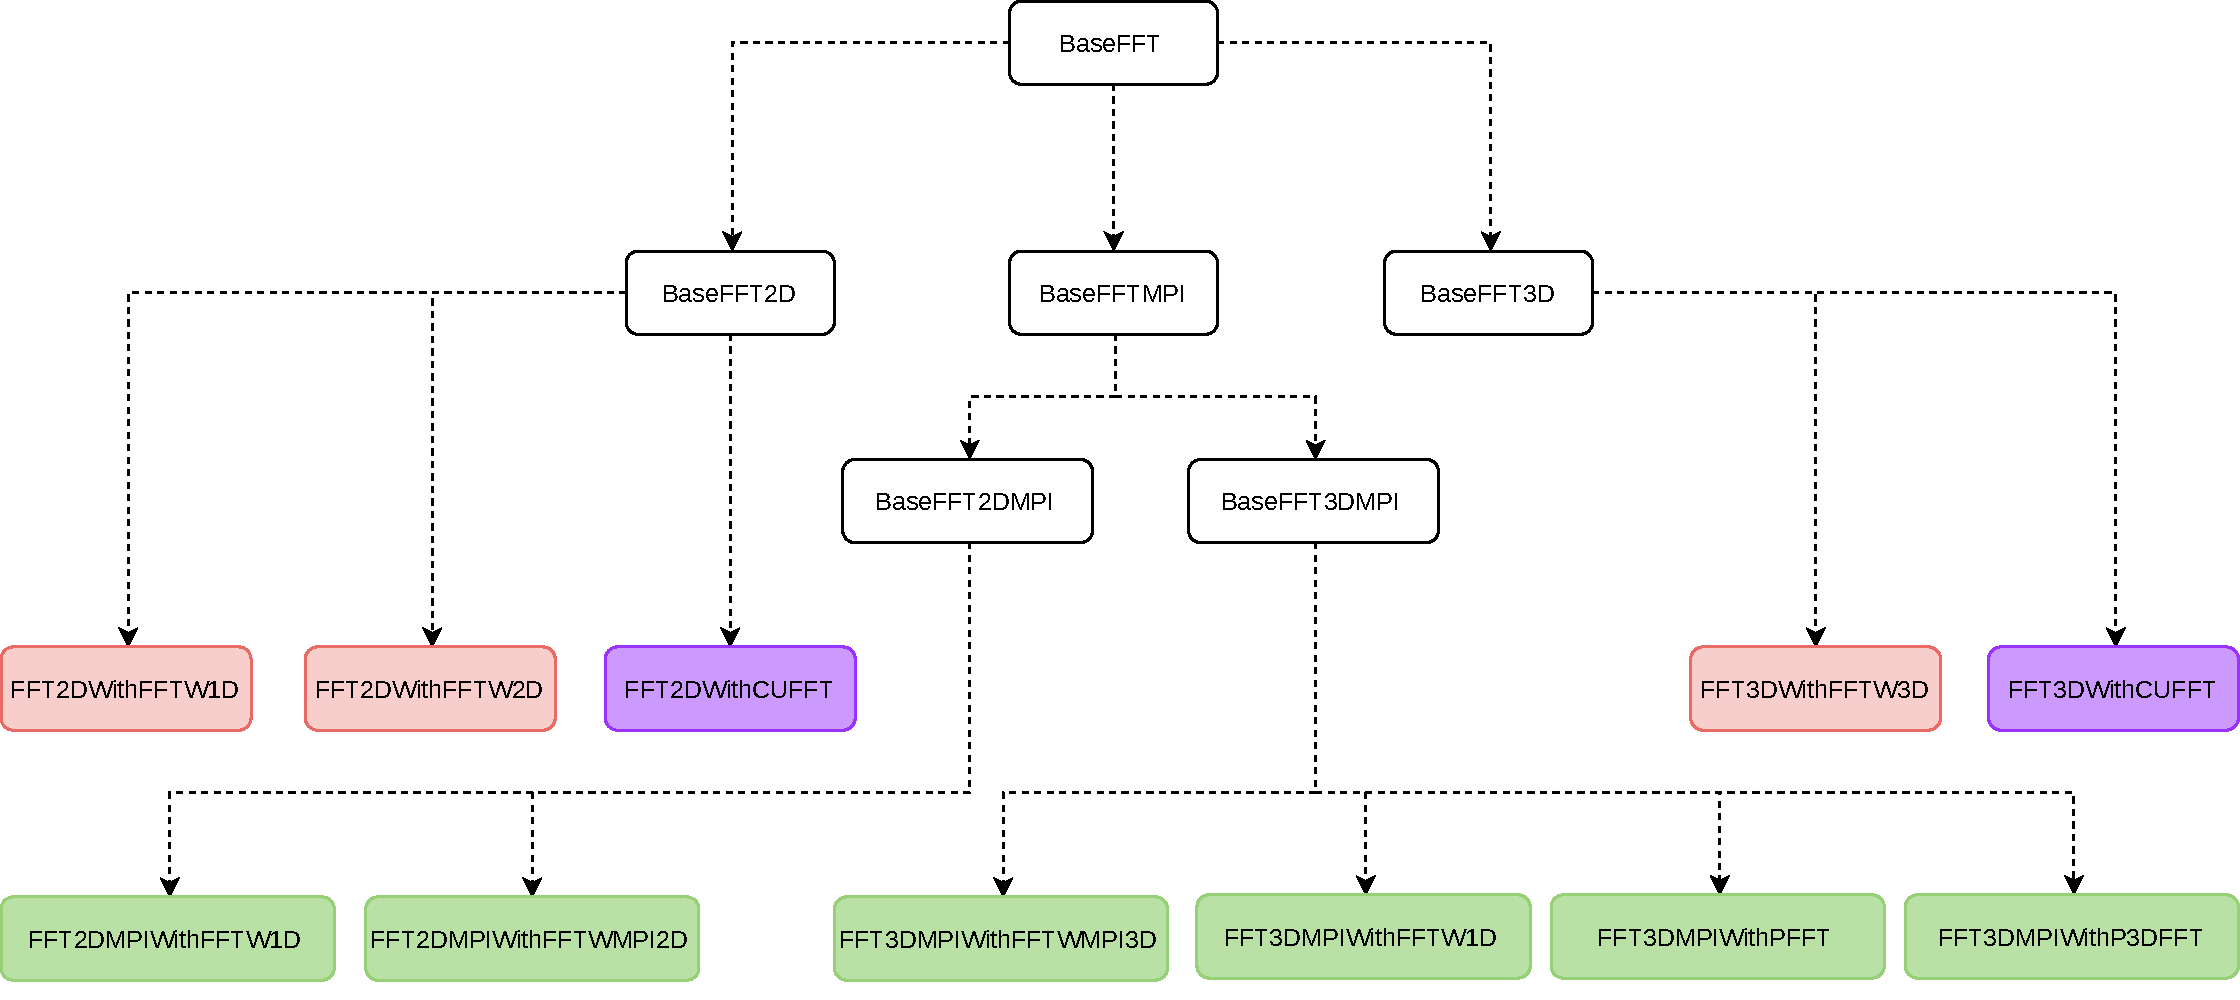
\includegraphics[width=\linewidth]{Pyfig/fig_classes}
  \caption{Class hierarchy demonstrating object-oriented approach. The
    sequential classes are shown in red, the CUDA-based classes in magenta and
    the MPI-based classes in green. The arrows represent inheritance from
    parent to child class.
  }\label{fig:classes}
\end{figure}

The C++ API is implemented as a hierarchy of classes as shown in
Fig.~\ref{fig:classes}.
%
The naming convention used for the classes (\codeinline{<Type of FFT>With<Name of
Library>}) is a cue for how these are functioning internally.
%
By utilizing inheritance, the classes share the same function names and syntax
defined in the \emph{base} classes, shown in white boxes in
Fig.~\ref{fig:classes}. Some examples of such functions are:

\begin{itemize}
  \item \codeinline{alloc\_array\_X}: Allocates array to store a physical array
    with real datatype for the current process.
  \item \codeinline{alloc\_array\_K}: Allocates array to store a spectral array
    with complex datatype  for the current process.
  \item \codeinline{init\_array\_X\_random}: Allocates and initializes a physical
    array with random values.
  \item \codeinline{test}: Run tests for a class by comparing mean and mean energy
    values in an array before and after a set of \codeinline{fft} and
    \codeinline{ifft} calls.
  \item \codeinline{bench}: Benchmark the \codeinline{fft} and
    \codeinline{ifft} methods for certain number of iterations.
\end{itemize}

Remaining methods which are specific to a library are defined in the
corresponding child classes, depicted in coloured boxes in
Fig.~\ref{fig:classes}, for example:

\begin{itemize}
  \item \codeinline{are\_parameters\_bad}: Verifies whether the global array
    shape can be decomposed with the number of MPI processes available or not.
    If the parameters are compatible, the method returns \codeinline{false}.
    This method is called prior to initializing the class.
  \item \codeinline{fft} and \codeinline{ifft}: Forward and inverse FFT
    methods.
\end{itemize}

Let us illustrate with a trivial example, wherein we initialize the FFT with a
random physical array, and perform a set of \codeinline{fft} and \codeinline{ifft}
operations.
\begin{minted}[fontsize=\footnotesize]{cpp}
#include <iostream>
using namespace std;

#include <fft3dmpi_with_fftwmpi3d.h>
// #include <fft3dmpi_with_p3dfft.h>

int main(int argc, char **argv) {
  int N0 = N1 = N2 = 32;
  // MPI-related
  int nb_procs = 4;
  MPI_Init(&argc, &argv);
  MPI_Comm_size(MPI_COMM_WORLD, &(nb_procs));

  myreal* array_X;
  mycomplex* array_K;

  FFT3DMPIWithFFTWMPI3D o(N0, N1, N2);
  // FFT3DMPIWithP3DFFT o(N0, N1, N2);

  o.init_array_X_random(array_X);
  o.alloc_array_K(array_K);
  o.fft(array_X, array_K);
  o.ifft(array_K, array_X);
  MPI_Finalize();
  return 0;
}
\end{minted}

As suggested through comments above, in order to switch the FFT library, the
user only needs to change the header file and the class name. An added
advantage is that, the user does not need to bother about the domain
decomposition while declaring and allocating the arrays. A few more helper
functions are available with the FFT classes, such as functions to compute the
mean value and energies in the array. These are demonstrated with examples in
the documentation.\footnote{%
\url{https://fluidfft.readthedocs.io/en/latest/examples/cpp.html}.}
%
Detailed information regarding the C++ classes and its member functions are
also included in the online documentation\footnote{%
\url{https://fluidfft.readthedocs.io/en/latest/doxygen/index.html}.}.

\subsection{Python API} Similar to other packages in the FluidDyn project,
\fluidpack{fft} also uses an object-oriented approach, providing FFT classes.
%
This is in contrast with the approach adopted by \pack{numpy.fft} and \pack{%
scipy.fftpack} which provides functions instead, with which the user has to
figure out the procedure to design the input values and to use the return
values, from the documentation.
%
In \fluidpack{fft}, the Python API wraps all the functionalities of its C++
counterpart and offers a richer experience through an accompanying
operator class.

As a short example, let us try to calculate the gradient of a plane sine-wave
using spectral methods, mathematically described as follows:

\begin{align*}
  u(x,y) &=
    \sin(x + y) &\forall x,y \in \left[0, L \right] \\
  \hat u(k_x,k_y) &=
    \frac{1}{L^2}
    \int_0^{L}\int_0^{L}
    u(x,y) \exp(ik_x x + ik_y y) dx dy \\
  \nabla u(x,y) &=
    \sum_{k_x} \sum_{k_y}
    i\mathbf{k}
    \hat u(k_x,k_y) \exp(-ik_x x - ik_y y)
\end{align*}
%
where $k_x$, $k_y$ represent the wavenumber corresponding to $x$ and $y$ directions,
and $\mathbf{k}$ is the wavenumber vector.

The equivalent pseudo-spectral implementation in \fluidpack{fft} is as follows:
\begin{minted}[fontsize=\footnotesize]{python}
  from fluidfft.fft2d.operators import OperatorsPseudoSpectral2D, pi
  from numpy import sin

  nx = ny = 100
  lx = ly = 2 * pi

  oper = OperatorsPseudoSpectral2D(nx, ny, lx, ly, fft="fft2d.with_fftw2d")

  u = sin(oper.XX + oper.YY)
  u_fft = oper.fft(u)
  px_u_fft, py_u_fft = oper.gradfft_from_fft(u_fft)
  px_u = oper.ifft(px_u_fft)
  py_u = oper.ifft(py_u_fft)
  grad_u = (px_u, py_u)
\end{minted}

A parallelized version of the code above will work out of the box, simply by
replacing the FFT class with an MPI-based FFT class, for instance
\codeinline{fft2d.with\_fftwmpi2d}. One can also let \fluidpack{fft} automatically
choose an appropriate FFT class by instantiating the operator class with
\codeinline{fft=None} or \codeinline{fft="default"}. Even if one finds the methods
in the operator class to be lacking, one can inherit the class and easily create a
new method, for instance using the wavenumber arrays, \codeinline{oper.KX} and
\codeinline{oper.KY}.  Arguably, a similar implementation with other available
packages would require the know-how on how FFT arrays are allocated in the memory,
normalized, decomposed in parallel and so on.
%
Moreover, the FFT and the operator classes contain objects describing the shapes
of the real and complex arrays and how the data is shared between processes.
%
A more detailed introduction on how
to use \fluidpack{fft} and available functions can be found in the
tutorials\footnote{%
\url{https://fluidfft.readthedocs.io/en/latest/tutorials.html}.}.

Thus, we have demonstrated how, by using \fluidpack{fft}, a developer can
easily switch between FFT libraries.
%
Let us now turn our attention to how the code is organized. We shall also describe
how the source code is built, and linked with the supported libraries.

\subsection{Code organization}
\begin{figure}[htp]
  \centering
  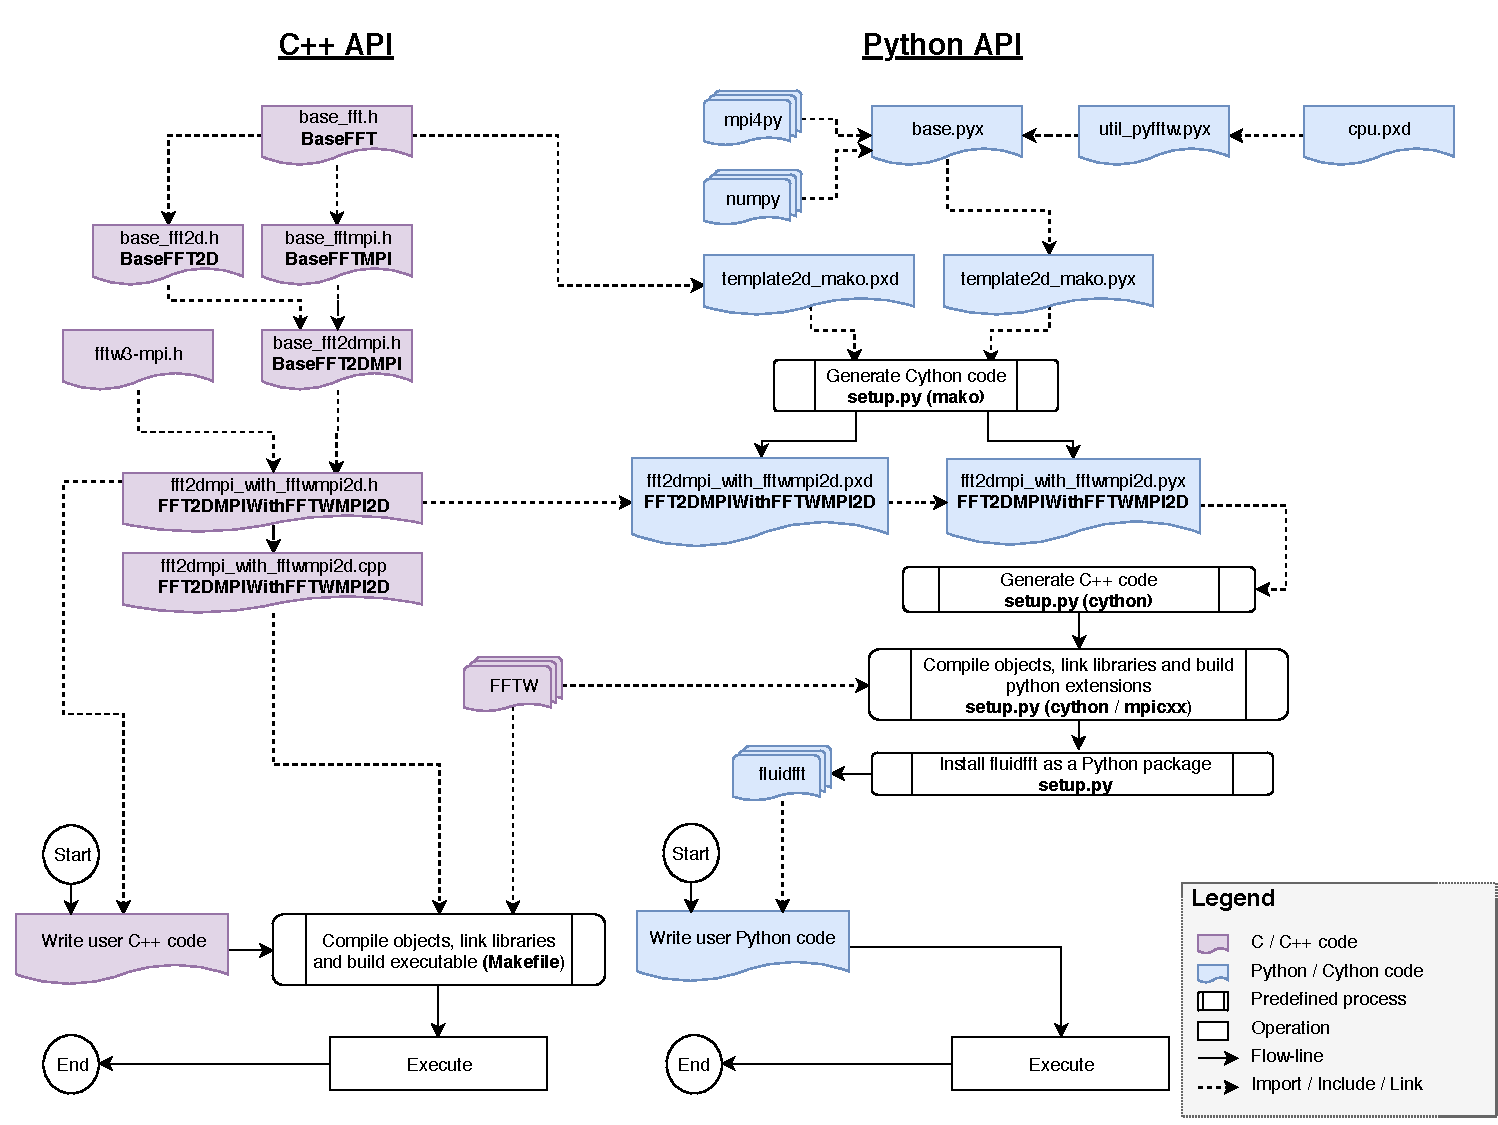
\includegraphics[width=0.96\linewidth]{Pyfig/fig_build_use}
  \caption{Flowchart illustrating how the C++ and Python API are built and used
  for one particular class, viz. \codeinline{FFT2DMPIWithFFTWMPI2D}. The dotted
  arrows in C++ part stand for include statements, demonstrating the class
  hierarchy and in the Python part indicate how different codes are imported. On
  the bottom, a smaller flowchart demonstrates how to use the API by writing user
  code.  }\label{fig:build_use}
\end{figure}

The internal architecture of \fluidpack{fft} can be visualized as layers.  Through
Fig.~\ref{fig:build_use}, we can see how these layers are linked together forming
the API for C++ and Python development. For simplicity, only one FFT class is
depicted in the figure, namely \codeinline{FFT2DMPIWithFFTWMPI2D}, which wraps
\libpack{FFTW}'s parallelized 2D FFT implementation. The C++ API is accessed by
importing the appropriate header file and building the user code with a Makefile,
an example of which is available \href{%
https://fluidfft.readthedocs.io/en/latest/examples/cpp.html}{%
in the documentation}.

The Python API is built automatically when \fluidpack{fft} is
installed\footnote{%
\href{https://fluidfft.readthedocs.io/en/latest/install.html}{Detailed steps
for installation} are provided in the documentation.}.
%
It first generates the Cython source code as a pair of \codeinline{.pyx} and
\codeinline{.pxd} files containing a class wrapping its C++
counterpart\footnote{Uses an approach similar to guidelines \href{%
    https://cython.readthedocs.io/en/latest/src/userguide/wrapping_CPlusPlus.html}{%
``Using C++ in Cython''} in the Cython documentation.}.
%
The Cython files are produced from template files (specialized for the 2D and
3D cases) using the template library \mako.
%
Thereafter, \pack{Cython} \citep{behnel_cython2011} generates C++ code with
necessary Python bindings, which are then built in the form of extensions or
dynamic libraries importable in Python code. All the built extensions are then
installed as a Python package named \fluidpack{fft}.

A helper function \codeinline{fluidfft.import\_fft\_class} is provided with the
package to simply import the FFT class. However, it is more convenient and
recommended to use an operator class, as described in the example for Python
API.\@ Although the operator classes can function as pure Python code, some of
its critical methods can be compiled, if \pack{Pythran}
\citep{guelton2018pythran} is available during installation of
\fluidpack{fft}. We will show towards the end of this section that by using
\pack{Pythran}, we reach the performance of the equivalent Fortran code.

To summarize, \fluidpack{fft} consists of the following layers:
\begin{itemize}

\item One C++ class per FFT library derived from a hierarchy of C++ classes
as shown in Fig.~\ref{fig:classes}.

\item \pack{Cython} wrappers of the C++ classes with their unit test cases.

\item Python operator classes (2D and 3D) to write code independently of the
library used for the computation of the FFT and with some mathematical helper
methods. These classes are accompanied by unit test cases.

\item \pack{Pythran} functions to speedup critical methods in the Python
operator classes.

\end{itemize}

Command-line utilities (\codeinline{fluidfft-bench} and
\codeinline{fluidfft-bench-analysis}) are also provided with the \fluidpack{fft}
installation to run benchmarks and plot the results. In the next subsection, we
shall look at some results by making use of these utilities on three computing
clusters.

\subsection{Performance}

\paragraphbf{Scalability tests using \codeinline{fluidfft-bench}}

% Simple!! Few cases. Few clusters. Figures obtained with
% fluidfft-bench-analysis

Scalability of \fluidpack{fft} is measured in the form of strong scaling speedup,
defined in the present context as:
\begin{equation*}
S_\alpha(n_p) = \frac
{[\mathrm{Time\ elapsed\ for\ } N \mathrm{\ iterations\ with\ }n_{p,\min}\mathrm{\ processes}]_{\mathrm{fastest}}
\times n_{p,\min}}
{[\mathrm{Time\ elapsed\ for\ } N \mathrm{\ iterations\ with\ } n_p \mathrm{\
processes}]_\alpha}
\label{eq:speedup}
\end{equation*}

where $n_{p,\min}$ is the minimum number of processes employed for a specific
array size and hardware. The subscripts, $\alpha$ denotes the FFT class used and
``fastest'' corresponds to the fastest result among various FFT classes.

To compute strong scaling the utility \codeinline{fluidfft-bench} is launched
as scheduled jobs on HPC clusters, ensuring no interference from background
processes. No hyperthreading was used.
%
We have used $N=20$ iterations for each run, with which we obtain sufficiently
repeatable results.
%
For a particular choice of array size, every FFT class available are
benchmarked for the two tasks, forward and inverse FFT. Three different function
variants are compared (see the legend in subsequent figures):

\begin{itemize}

\item \codeinline{fft\_cpp}, \codeinline{ifft\_cpp} (continuous lines): benchmark
of the C++ function from the C++ code. An array is passed as an argument to store
the result. No memory allocation is performed inside these functions.

\item \codeinline{fft\_as\_arg}, \codeinline{ifft\_as\_arg} (dashed lines):
benchmark of a Python method from Python. Similar to the C++ code, the second
argument of this method is an array to contain the result of the transform, so no
memory allocation is needed.

\item \codeinline{fft\_return}, \codeinline{ifft\_return} (dotted lines):
benchmark of a Python method from Python. No array is provided to the function to
contain the result, and therefore a numpy array is created and then returned by
the function.

\end{itemize}

On big HPC clusters, we have only focussed on 3D array transforms as benchmark
problems, since these are notoriously expensive to compute and require massive
parallelization.  The physical arrays used in all four 3D MPI based FFT classes
are identical in structure.  However, there are subtle differences, in terms of
how the domain decomposition and the allocation of the transformed array in the
memory are handled\footnote{Detailed discussion on \href{%
https://fluidfft.readthedocs.io/en/latest/ipynb/executed/tuto_fft3d_mpi_domain_decomp.html}{%
``FFT 3D parallel (MPI): Domain decomposition''} tutorial}.

Hereafter, for the sake of brevity, the FFT classes will be named in terms of the
associated library (For example, the class \codeinline{FFT3DMPIWithFFTW1D} is
named \codeinline{fftw1d}).  Let us go through the results\footnote{Saved at
\url{%
https://bitbucket.org/fluiddyn/fluidfft-bench-results}} plotted using
\codeinline{fluidfft-bench-analysis}.

\paragraph{Benchmarks on Occigen}

\href{https://www.top500.org/system/178465}{Occigen} is a GENCI-CINES HPC
cluster which uses Intel Xeon CPU E5--2690 v3 (2.6 GHz) processors with 24 cores
per node. The installation was performed using Intel C++ 17.2 compiler, Python
3.6.5, and OpenMPI 2.0.2.

\begin{figure}[htp!]
\centering
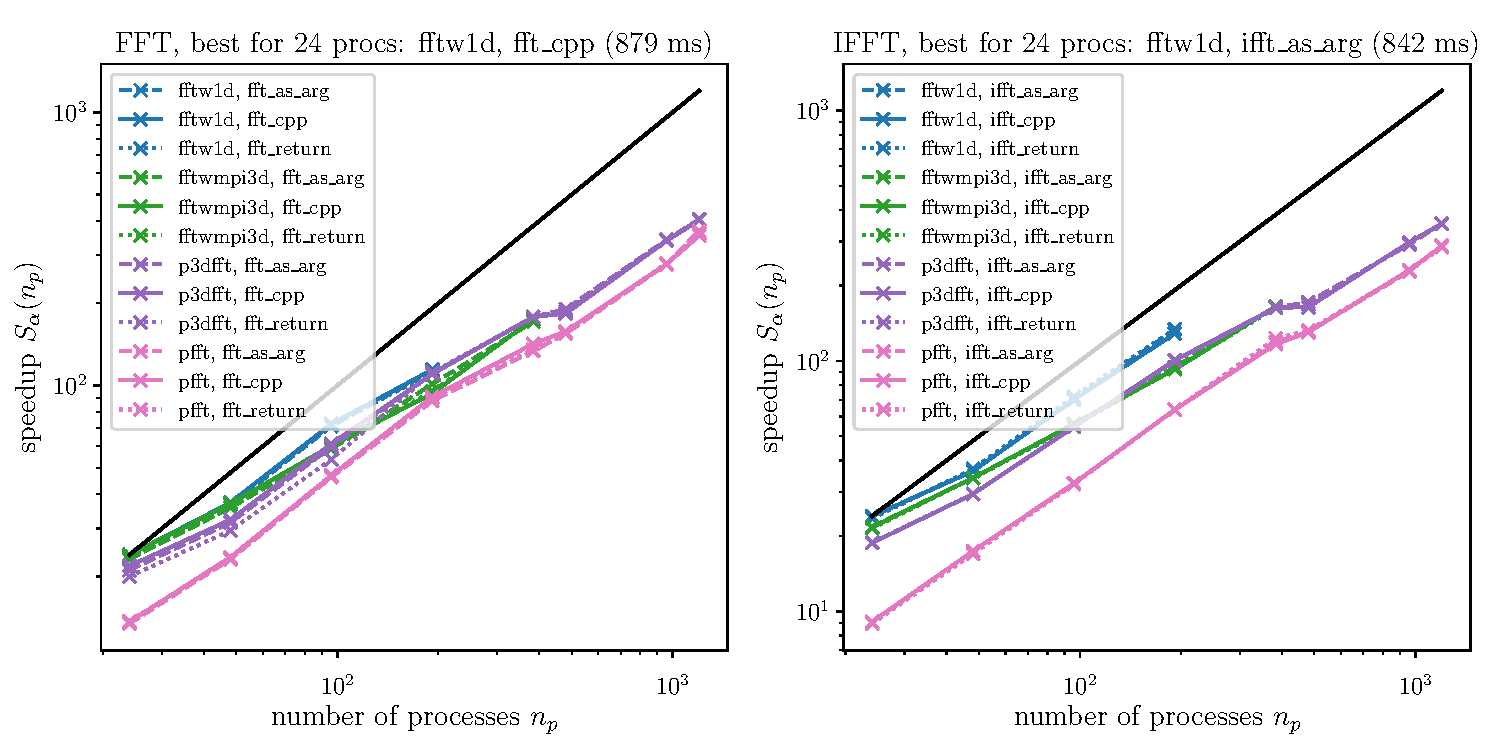
\includegraphics[width=\linewidth]{tmp/fig_occigen_384x1152x1152}
\caption{Speedup computed from the median of the elapsed times for 3D fft
(384$\times$1152$\times$1152, left: fft and right: ifft) on Occigen.}%
\label{fig:occigen384x1152x1152}
\end{figure}

Fig.~\ref{fig:occigen384x1152x1152} demonstrates the strong scaling performance
of a cuboid array sized $384\times1152\times1152$. This case is particularly
interesting since for FFT classes implementing 1D domain decomposition
(\codeinline{fftw1d} and \codeinline{fftwmpi3d}), the processes are spread on
the first index for the physical input array. This restriction is as a result
of some \libpack{FFTW} library internals and design choices adopted in
\fluidpack{fft}. This limits \codeinline{fftw1d} (our own MPI implementation
using MPI types and 1D transforms from FFTW) to 192 cores and
\codeinline{fftwmpi3d} to 384 cores. The latter can utilize more cores since it
is capable of working with empty arrays, while sharing some of the
computational load.
%
The fastest methods for relatively
low and high number of processes are \codeinline{fftw1d} and
\codeinline{p3dfft} respectively for the present case.

The benchmark is not sufficiently accurate to measure the cost of calling the
functions from Python (difference between continuous and dashed lines,
i.e. between pure C++ and the \codeinline{as\_arg} Python method) and even the
creation of the numpy array (difference between the dashed and the dotted line,
i.e. between the \codeinline{as\_arg} and the \codeinline{return} Python
methods).


\begin{figure}[htp!]
\centering
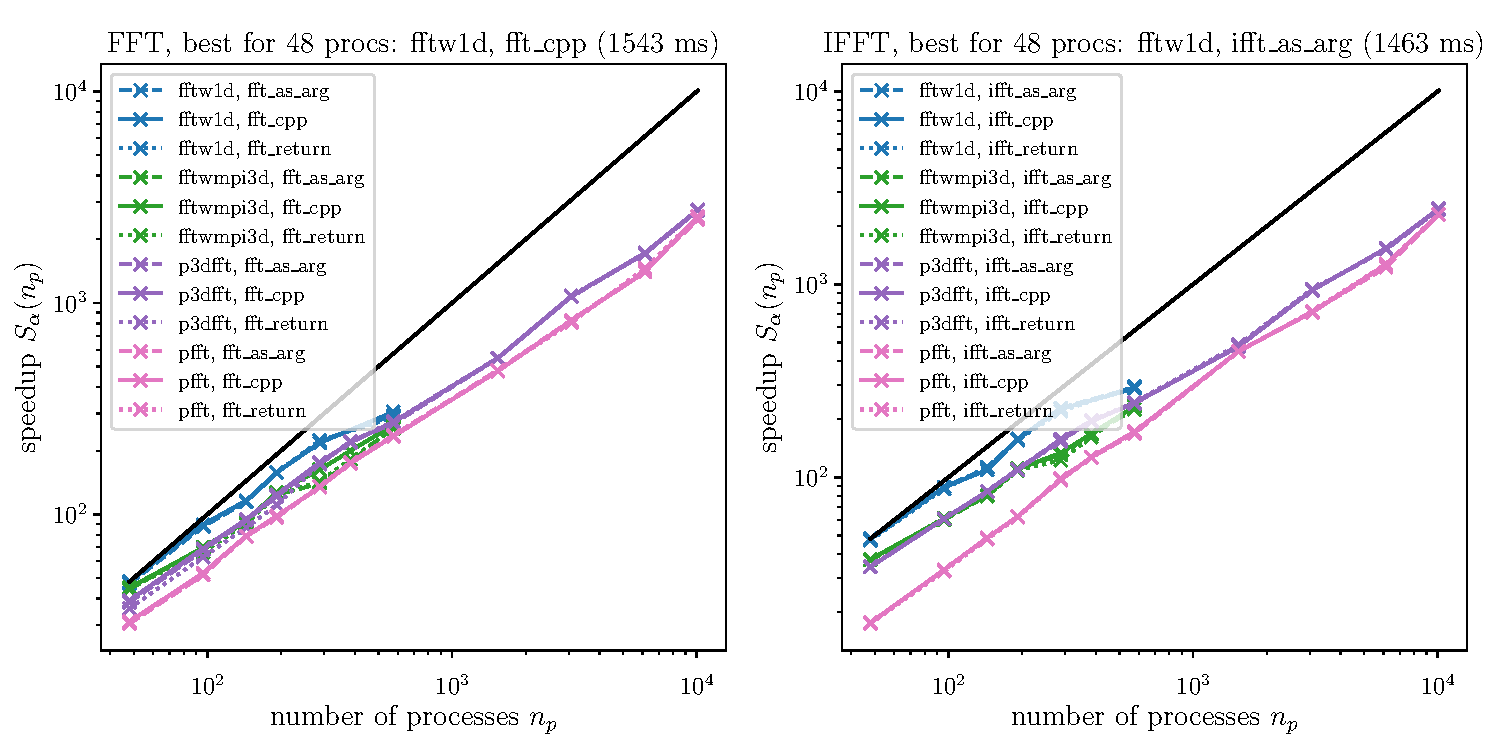
\includegraphics[width=\linewidth]{tmp/fig_occigen_1152x1152x1152}
\caption{Speedup computed from the median of the elapsed times for 3D fft
(1152$\times$1152$\times$1152, left: fft and right: ifft) on Occigen.}
\label{fig:occigen1152x1152x1152}
\end{figure}

Fig.~\ref{fig:occigen1152x1152x1152} demonstrates the strong scaling
performance of a cubical array sized $1152\times1152\times1152$. For this
resolution as well, \codeinline{fftw1d} is the fastest method when using only
few cores and it can not be used for more that 192 cores. The faster library
when using more cores is also \codeinline{p3dfft}. This also shows that
\fluidpack{fft} can effectively scale for over 10,000 cores with a significant
increase in speedup.


\paragraph{Benchmarks on Beskow}

\href{ https://www.pdc.kth.se/hpc-services/computing-systems}{Beskow} is a Cray
machine maintained by SNIC at PDC, Stockholm. It runs on Intel(R) Xeon(R) CPU
E5-2695 v4 (2.1 GHz) processors with 36 cores per node. The installation was
done using Intel C++ 18 compiler, Python 3.6.5 and CRAY-MPICH 7.0.4.

\begin{figure}[htp!]
\centering
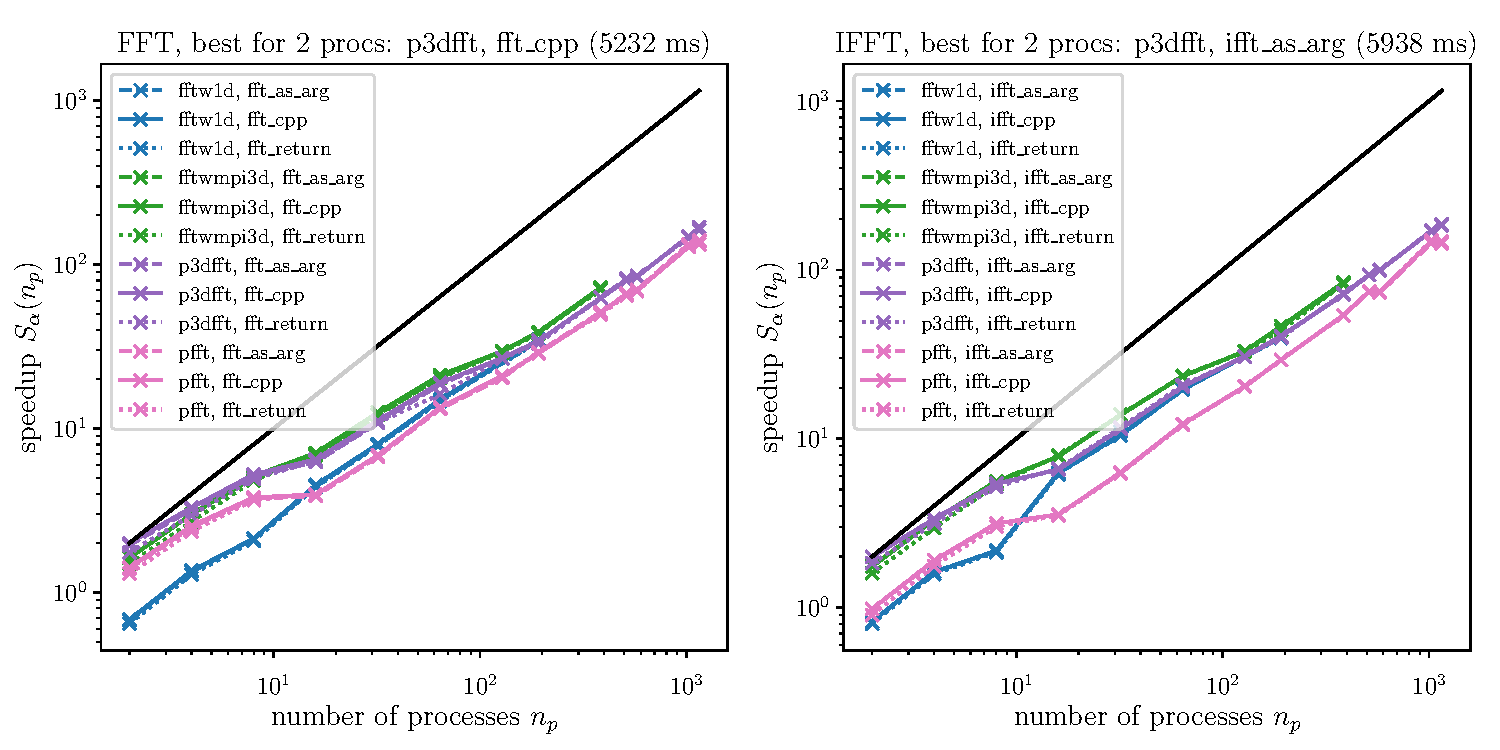
\includegraphics[width=\linewidth]{tmp/fig_beskow_384x1152x1152}
\caption{Speedup computed from the median of the elapsed times for 3D fft
(384$\times$1152$\times$1152, left: fft and right: ifft) on Beskow.}
\label{fig:beskow384x1152x1152}
\end{figure}

In Fig.~\ref{fig:beskow384x1152x1152}, the strong scaling results of the cuboid
array can be observed. In this set of results we have also included intra-node
scaling, wherein there is no latency introduced due to typically slower
node-to-node communication. The fastest library for very low (below 16) and
very high (above 384) number of processes in this configuration is
\codeinline{p3dfft}. For moderately high number of processes (16 and above) the
fastest library is \codeinline{fftwmpi3d}. Here too, we notice that
\codeinline{fftw1d} is limited to 192 cores and \codeinline{fftwmpi3d} to 384
cores, for reasons mentioned earlier.

A striking difference when compared with Fig.~\ref{fig:occigen384x1152x1152} is
that \codeinline{fftw1d} is not the fastest of the four classes in this machine.
One can only speculate that this could be a consequence of the differences in MPI
library and hardware which has been employed. This also emphasises the need to
perform benchmarks when using an entirely new configuration.

\begin{figure}[htp!]
\centering
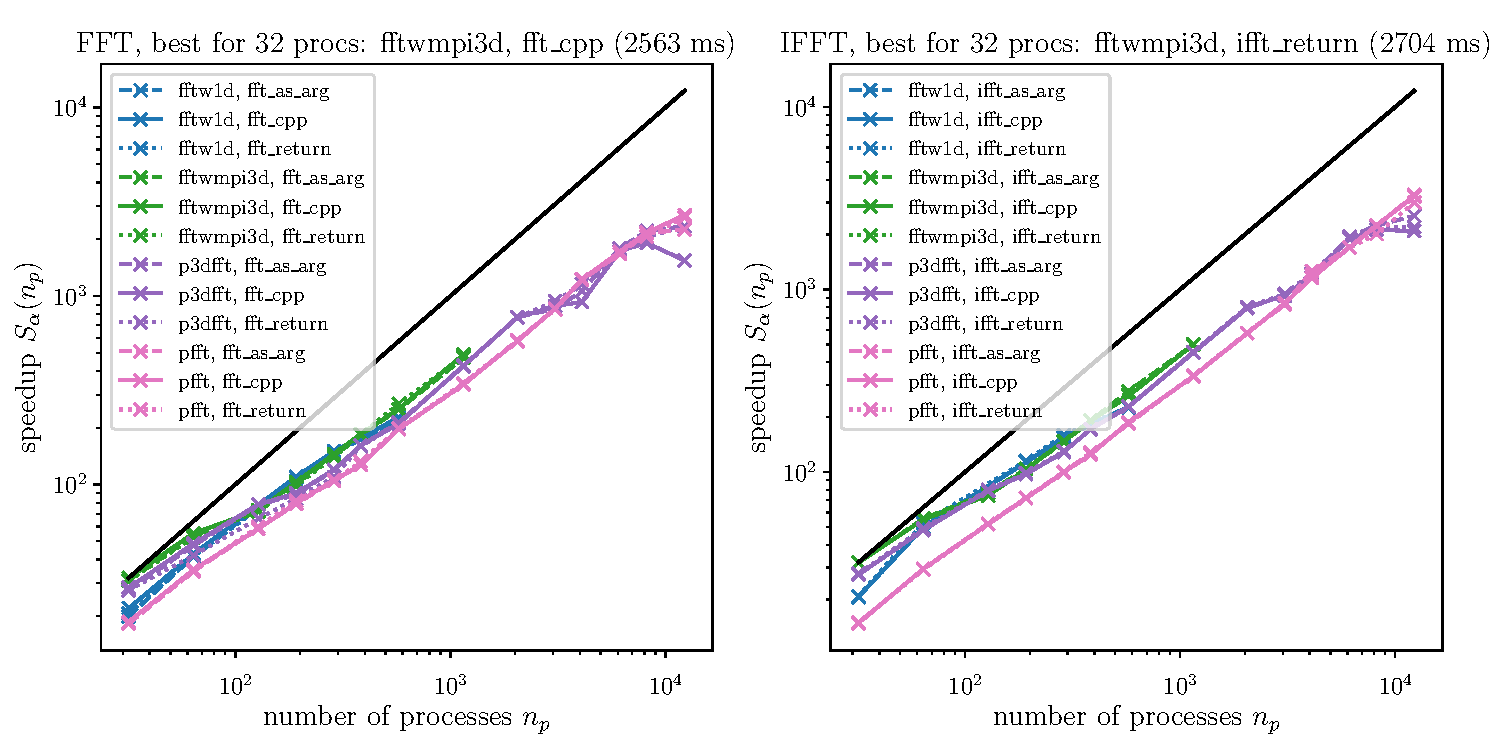
\includegraphics[width=\linewidth]{tmp/fig_beskow_1152x1152x1152}
\caption{Speedup computed from the median of the elapsed times for 3D fft
(1152$\times$1152$\times$1152, left: fft and right: ifft) on Beskow.}
\label{fig:beskow1152x1152x1152}
\end{figure}

The strong scaling results of the cubical array on Beskow are displayed on
Fig.~\ref{fig:beskow1152x1152x1152}, wherein we restrict to inter-node
computation.  We observe that the fastest method for low number of processes is
again, \codeinline{fftwmpi3d}. When high number of processes (above 1000)
are utilized, initially \codeinline{p3dfft} is the faster methods as before,
but with 3000 and above processes, \codeinline{pfft} is comparable in speed and
sometimes faster.

\paragraph{Benchmarks on a LEGI cluster}

Let us also analyse how \fluidpack{fft} scales on a computing cluster
maintained at an institutional level, named Cluster8 at \href{%
http://www.legi.grenoble-inp.fr}{LEGI}, Grenoble. This cluster functions using
Intel Xeon CPU E5-2650 v3 (2.3 GHz) with 20 cores per node and \fluidpack{fft}
was installed using a toolchain which comprises of gcc 4.9.2, Python 3.6.4 and
OpenMPI 1.6.5 as key software components.

\begin{figure}[htp!]
\centering
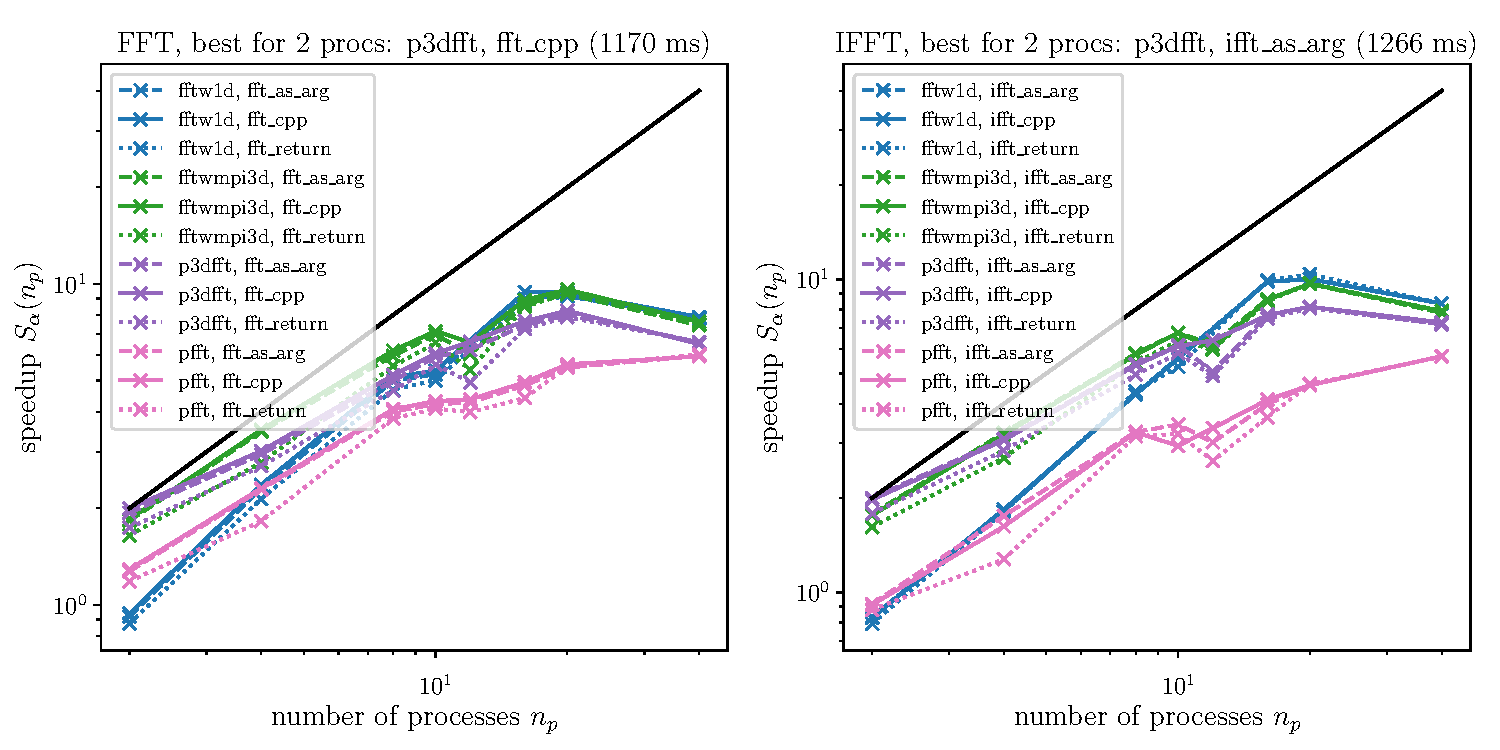
\includegraphics[width=\linewidth]{tmp/fig_legi_cluster8_320x640x640}
\caption{Speedup computed from the median of the elapsed times for 3D fft
(320$\times$640$\times$640) at LEGI on cluster8.}
\label{fig:cluster8:320x640x640}
\end{figure}

In Fig.~\ref{fig:cluster8:320x640x640} we observe that the strong scaling for an
array shape of $320\times640\times640$ is not far from the ideal linear trend. The
fastest library is \codeinline{fftwmpi3d} for this case.  As expected from FFT
algorithms, there is a slight drop in speedup when the array size is not exactly
divisible by the number of processes, i.e.\ with 12 processes. The speedup
declines rapidly when more than one node is employed (above 20 processes). This
effect can be attributed to the latency introduced by inter-node communications, a
hardware limitation of this cluster (10 Gb/s).

\begin{figure}[htp!]
\centering
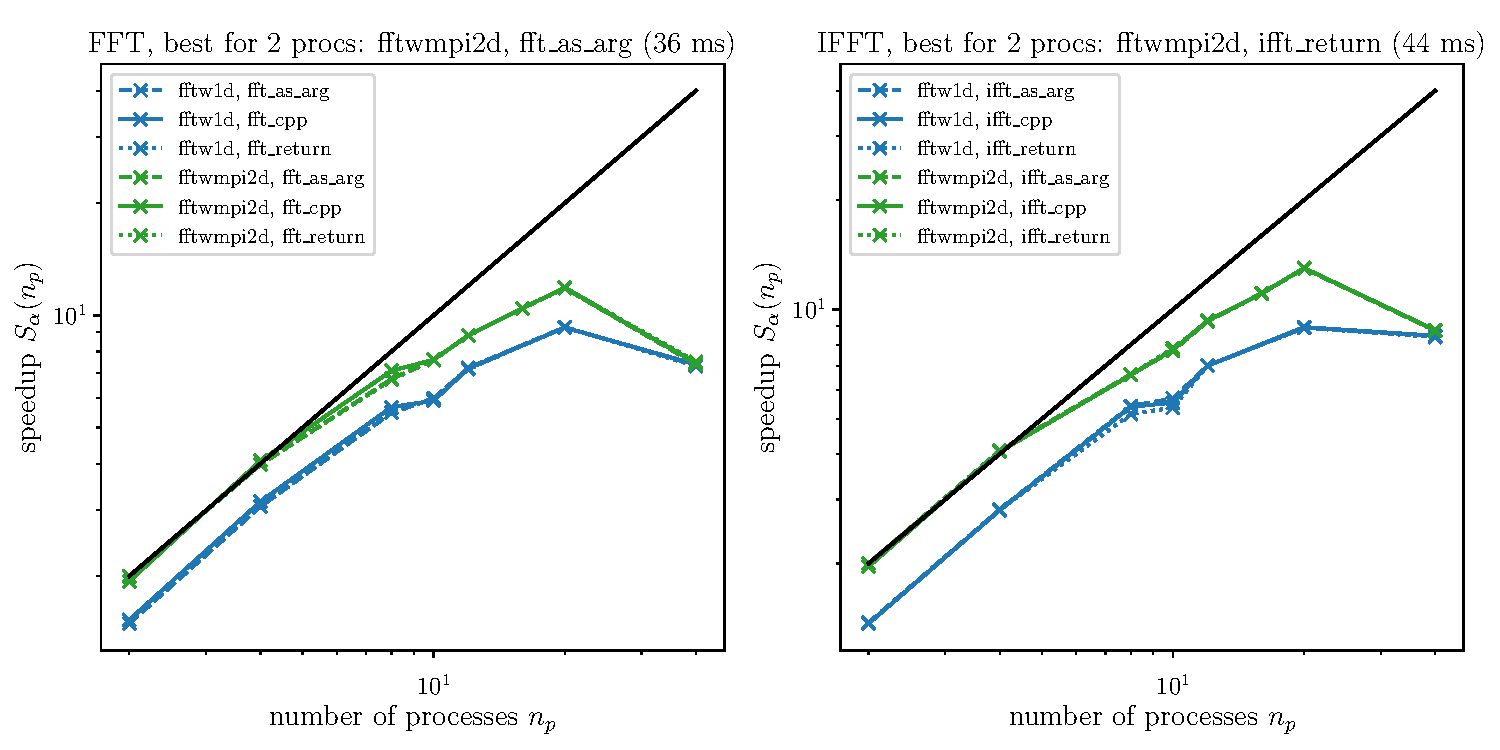
\includegraphics[width=\linewidth]{tmp/fig_legi_cluster8_2160x2160}
\caption{Speedup computed from the median of the elapsed times for 2D fft
(2160$\times$2160) at LEGI on cluster8.}
\label{fig:cluster8:2160x2160}
\end{figure}

We have also analysed the performance of 2D MPI enabled FFT classes on the same
machine using an array shaped $2160\times2160$ in
Fig.~\ref{fig:cluster8:2160x2160}. The fastest library is
\codeinline{fftwmpi2d}. Both \codeinline{fftw1d} and \codeinline{fftwmpi2d}
libraries display near-linear scaling, except when more than one node is used
and the performance tapers off.

As a conclusive remark on scalability, a general rule of thumb should be to use
1D domain decomposition when only very few processors are employed. For massive
parallelization, 2D decomposition is required to achieve good speedup without
being limited by the number of processors at disposal. We have thus shown that
overall performance of the libraries interfaced by \fluidpack{fft} are quite
good, and there is no noticeable drop in speedup when the Python API is used.
%
This benchmark analysis also shows that the fastest FFT implementation depends
on the size of the arrays and on the hardware.
%
Therefore, an application build upon \fluidpack{fft} can be efficient for
different sizes and machines.


\paragraphbf{Microbenchmark of critical ``operator'' functions}

As already mentioned, we use \pack{Pythran} \citep{guelton2018pythran} to
compile some critical ``operator'' functions.  In this subsection, we present a
microbenchmark for one simple task used in pseudo-spectral codes: projecting a
velocity field on a non-divergent velocity field.  It is performed in spectral
space, where it can simply be written as
\begin{minted}[fontsize=\footnotesize]{python}
# pythran export proj_out_of_place(
#     complex128[][][], complex128[][][], complex128[][][],
#     float64[][][], float64[][][], float64[][][], float64[][][])

def proj_out_of_place(vx, vy, vz, kx, ky, kz, inv_k_square_nozero):
    tmp = (kx * vx + ky * vy + kz * vz) * inv_k_square_nozero
    return vx - kx * tmp, vy - ky * tmp, vz - kz * tmp
\end{minted}
Note that, this implementation is ``out-of-place'', meaning that the result is
returned by the function and that the input velocity field (\codeinline{vx, vy,
vz}) is unmodified.
%
The comment above the function definition is a \pack{Pythran} annotation, which
serves as a type-hint for the variables used within the functions --- all
arguments being \pack{Numpy} arrays in this case.
%
\pack{Pythran} needs such annotation to be able to compile this code into
efficient machine instructions \emph{via} a C++ code.
%
Without \pack{Pythran} the annotation has no effect, and
of course, the function defaults to using Python with \pack{Numpy} to execute.

The array notation is well adapted and less verbose to express this simple
vector calculus.
%
Since explicit loops with indexing is not required, the computation with Python
and \pack{Numpy} is not extremely slow. Despite this being quite a favourable
case for \pack{Numpy}, the computation with \pack{Numpy} is not optimized
because, internally, it involves many loops (one per arithmetic operator) and
creation of temporary arrays.
%av: Have I understood correctly here with the clarifications: "internally" &
%   "arithmetic operator"?

\begin{figure}[htp]
\centering
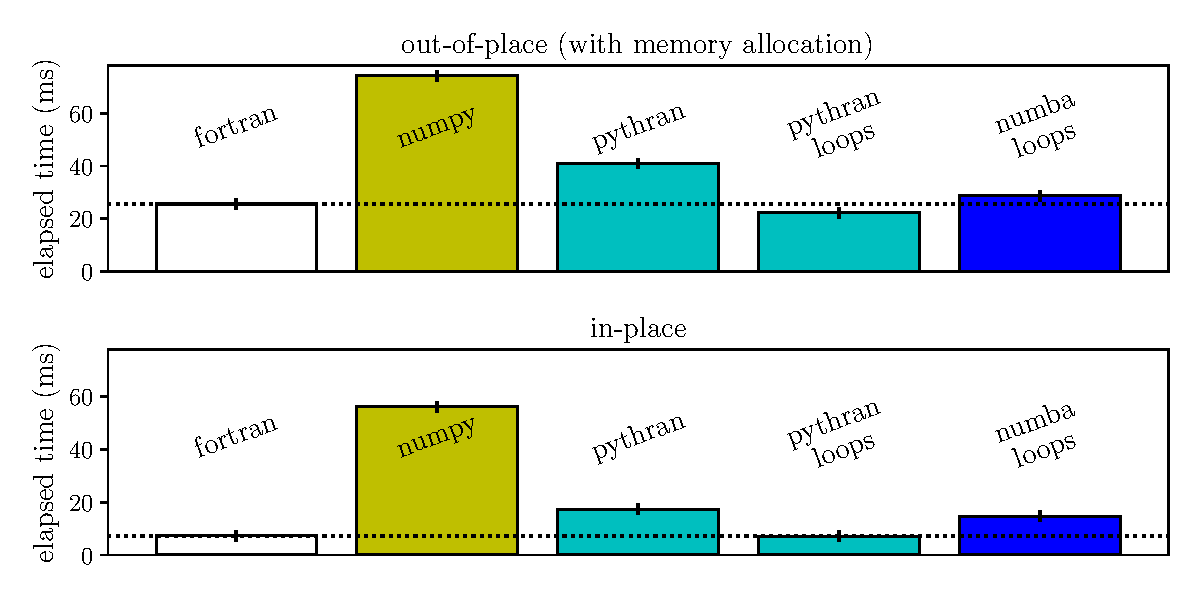
\includegraphics[width=\linewidth]{tmp/fig_microbench}
\caption{Elapsed time (smaller is better) for the projection function for
different implementations and tools.  The shape of the arrays is
$(128,\ 128,\ 65)$. The dotted lines indicate the times for Fortran for better
comparison.}
\label{fig:microbench}
\end{figure}

In the top axis of Fig.~\ref{fig:microbench}, we compare the elapsed times for
different implementations of this function.
%
For this out-of-place version, we used three different codes:
\begin{enumerate}
\item a Fortran code (not shown\footnote{The codes and a Makefile used for this
benchmark study are available in \href{%
https://bitbucket.org/fluiddyn/fluiddyn_paper/src/default/fluidfft/microbench/}{%
the repository of the article}.}) written with three nested explicit loops (one
per dimension). Note that as in the Python version we also allocate the memory
where the result is stored.
\item the simplest Python version shown above.
\item a Python version with three nested explicit loops:
% (code not shown).
\begin{minted}[fontsize=\footnotesize]{python}
# pythran export proj_out_of_place_loop(
#     complex128[][][], complex128[][][], complex128[][][],
#     float64[][][], float64[][][], float64[][][], float64[][][])

def proj_out_of_place_loop(vx, vy, vz, kx, ky, kz, inv_k_square_nozero):

    rx = np.empty_like(vx)
    ry = np.empty_like(vx)
    rz = np.empty_like(vx)

    n0, n1, n2 = kx.shape

    for i0 in range(n0):
        for i1 in range(n1):
            for i2 in range(n2):
                tmp = (kx[i0, i1, i2] * vx[i0, i1, i2]
                       + ky[i0, i1, i2] * vy[i0, i1, i2]
                       + kz[i0, i1, i2] * vz[i0, i1, i2]
                ) * inv_k_square_nozero[i0, i1, i2]

                rx[i0, i1, i2] = vx[i0, i1, i2] - kx[i0, i1, i2] * tmp
                ry[i0, i1, i2] = vz[i0, i1, i2] - kx[i0, i1, i2] * tmp
                rz[i0, i1, i2] = vy[i0, i1, i2] - kx[i0, i1, i2] * tmp

    return rx, ry, rz
\end{minted}
\end{enumerate}
For the version without explicit loops, we present the elapsed time for two
cases: (i) simply using Python (yellow bar) and (ii) using the Pythranized
function (first cyan bar).
%
For the Python version with explicit loops, we only present the results for (i)
the Pythranized function (second cyan bar) and (ii) the result of \pack{Numba}
(blue bar).
%
We do not show the result for \pack{Numba} for the code without explicit loops
because it is slower than \pack{Numpy}. We have also omitted the result for
\pack{Numpy} for the code with explicit loops because it is very inefficient.
%
The timing is performed upon tuning the computer using the package
\href{https://pypi.org/project/perf/}{\pack{perf}}.

We see that \pack{Numpy} is approximately three time slower than the Fortran
implementation (which as already mentioned contains the memory allocation).
%
Just using \pack{Pythran} without changing the code (first cyan bar), we save
nearly 50\% of the execution time but we are still significantly slower than
the Fortran implementation.
%
We reach the Fortran performance (even slightly faster) only by using
\pack{Pythran} with the code with explicit loops.
%
With this code, \pack{Numba} is nearly as fast (but still slower) without
requiring any type annotation.

Note that the exact performance differences depend on the hardware, the software
versions\footnote{Here, we use Python~3.6.4 (packaged by conda-forge),
\pack{Numpy}~1.13.3, \pack{Pythran}~0.8.5, \pack{Numba}~0.38, gfortran~6.3 and
clang~6.0.}, the compilers and the compilation options.
%
We use \codeinline{gfortran -O3 -march=native} for Fortran and
\codeinline{clang++ -O3 -march=native} for \pack{Pythran}\footnote{The results
with \codeinline{g++ -O3 -march=native} are very similar but tend to be slightly
slower.}.
%


Since allocating memory is expensive and we do not need the non-projected
velocity field after the call of the function, an evident optimization is to
put the output in the input arrays.  Such an ``in-place'' version can be written
with \pack{Numpy} as:
\begin{minted}[fontsize=\footnotesize]{python}
# pythran export proj_in_place(
#     complex128[][][], complex128[][][], complex128[][][],
#     float64[][][], float64[][][], float64[][][], float64[][][])

def proj_in_place(vx, vy, vz, kx, ky, kz, inv_k_square_nozero):
    tmp = (kx * vx + ky * vy + kz * vz) * inv_k_square_nozero
    vx -= kx * tmp
    vy -= ky * tmp
    vz -= kz * tmp
\end{minted}

As in the first version, we have included the \pack{Pythran} annotation.
%
We also consider an ``in-place'' version with explicit loops:
\begin{minted}[fontsize=\footnotesize]{python}
# pythran export proj_in_place_loop(
#     complex128[][][], complex128[][][], complex128[][][],
#     float64[][][], float64[][][], float64[][][], float64[][][])

def proj_in_place_loop(vx, vy, vz, kx, ky, kz, inv_k_square_nozero):

    n0, n1, n2 = kx.shape

    for i0 in range(n0):
        for i1 in range(n1):
            for i2 in range(n2):
                tmp = (kx[i0, i1, i2] * vx[i0, i1, i2]
                       + ky[i0, i1, i2] * vy[i0, i1, i2]
                       + kz[i0, i1, i2] * vz[i0, i1, i2]
                ) * inv_k_square_nozero[i0, i1, i2]

                vx[i0, i1, i2] -= kx[i0, i1, i2] * tmp
                vy[i0, i1, i2] -= ky[i0, i1, i2] * tmp
                vz[i0, i1, i2] -= kz[i0, i1, i2] * tmp

\end{minted}
Note that this code is much longer and clearly less readable than the version
without explicit loops.  This is however the version which is used in
\pack{fluidfft} since it leads to faster execution.

The elapsed time for these in-place versions and for an equivalent Fortran
implementation are displayed in the bottom axis of Fig.~\ref{fig:microbench}.
%
The ranking is the same as for the out-of-place versions and \pack{Pythran} is also
the faster solution.
%
However, \pack{Numpy} is even more slower (7.8 times slower than \pack{Pythran}
with the explicit loops) than for the out-of-place versions.

From this short and simple microbenchmark, we can infer four main points:
\begin{itemize}
\item Memory allocation takes time!  In Python, memory management is automatic
and we tend to forget it.  An important rule to write efficient code is to
reuse the buffers already allocated as much as possible.

\item Even for this very simple case quite favorable for \pack{Numpy} (no indexing
or slicing), \pack{Numpy} is three to eight time slower than the Fortran
implementations. As long as the execution time is small or that the
function represents a small part of the total execution time, this is not an
issue. However, in other cases, Python-\pack{Numpy} users need to consider
other solutions.

\item \pack{Pythran} is able to speedup the \pack{Numpy} code without explicit
loops and is as fast as Fortran (even slightly faster in our case) for the
codes with explicit loops.

\item \pack{Numba} is unable to speedup the \pack{Numpy} code.
%
It gives very interesting performance for the version with explicit loops
without any type annotation but the result is significantly slower than with
\pack{Pythran} and Fortran.
\end{itemize}

For the aforementioned reasons, we have preferred \pack{Pythran} to compile
optimized ``operator'' functions that complement the FFT classes. Although with
this we obtain remarkable performance, there is still room for some
improvement, in terms of logical implementation and allocation of arrays. For
example, applications such as CFD simulations often deals with non-linear terms
which require dealiasing. The FFT classes of \fluidpack{fft}, currently
allocates the same number of modes in the spectral array so as to transform the
physical array. Thereafter, we apply dealiasing by setting zeros to wavenumbers
which are larger than, say, two-thirds of the maximum wavenumber. Instead, we
could take into account dealiasing in the FFT classes to save some memory and
computation time\footnote{See
\href{https://bitbucket.org/fluiddyn/fluidfft/issues/21/}{fluidfft issue 21}.}.

\section{Quality control}

% \textcolor{blue}{Detail the level of testing that has been carried out on the
% code (e.g. unit, functional, load etc.), and in which environments. If not
% already included in the software documentation, provide details of how a user
% could quickly understand if the software is working (e.g. providing examples of
% running the software with sample input and output data). }

The package \fluidpack{fft} currently supplies unit tests covering 90\% of its
code.  These unit tests are run regularly through continuous integration on Travis
CI with the most recent releases of \fluidpack{fft}'s dependencies and on
Bitbucket Pipelines inside a static
\href{https://hub.docker.com/u/fluiddyn}{Docker container}.  The tests are run
using standard Python interpreter with all supported versions.

For \fluidpack{fft}, the code coverage results are displayed at
\href{https://codecov.io/bb/fluiddyn/fluidfft}{Codecov}.  Using third-party
packages \pack{coverage} and \pack{tox}, it is straightforward to bootstrap the
installation with dependencies, test with multiple Python versions and combine the
code coverage report, ready for upload. It is also possible to run similar
isolated tests using \pack{tox} or coverage analysis using \pack{coverage} in a
local machine.  Up-to-date build status and coverage status are displayed on the
landing page of the Bitbucket repository.  Instructions on how to run unit tests,
coverage and lint tests are included in the documentation.

We also try to follow a consistent code style as recommended by PEP (Python
enhancement proposals) 8 and 257. This is also inspected using lint checkers such
as \codeinline{flake8} and \codeinline{pylint} among the developers.  The Python
code is regularly cleaned up using the code formatter \codeinline{black}.


\section{(2) Availability}
\vspace{0.5cm}
\section{Operating system}

% \textcolor{blue}{Please include minimum version compatibility.}

Windows and any POSIX based OS, such as GNU/Linux and macOS.

\section{Programming language}

% \textcolor{blue}{Please include minimum version compatibility.}

Python 2.7, 3.5 or above. For the next versions, we will
\href{https://python3statement.org/}{drop Python 2.7 support and Python $>=$
3.6 will be required}.
%
Note that while Cython and Pythran both use the C API of CPython, \fluidpack{fft}
has been successfully tested on PyPy 6.0.
%
A C++11 supporting compiler, while not mandatory for the C++ API or Cython
extensions of \fluidpack{fft}, is recommended to be able to use Pythran extensions.

\section{Dependencies}

% \textcolor{blue}{E.g. libraries, frameworks, incl. minimum version
% compatibility.}
C++ API:
\begin{itemize}
  \item{\bf Optional:} \pack{OpenMPI} or equivalent, \libpack{FFTW},
    \libpack{P3DFFT}, \libpack{PFFT} and \libpack{cuFFT} libraries.
\end{itemize}

Python API:

\begin{itemize}
\item {\bf Minimum:} \fluidpack{dyn}, \pack{Numpy}, \pack{Cython}, and
  \pack{mako}\ or \pack{Jinja2}; \libpack{FFTW} library.
\item {\bf Optional:} \pack{mpi4py} and \pack{Pythran}; \libpack{P3DFFT},
  \libpack{PFFT} and \libpack{cuFFT} libraries.
\end{itemize}


\section{List of contributors}

% \textcolor{blue}{Please list anyone who helped to create the software (who may
% also not be an author of this paper), including their roles and affiliations.}

\begin{itemize}
\item Pierre Augier (LEGI): creator of the FluidDyn project and of
\fluidpack{fft}.
\item Cyrille Bonamy (LEGI): C++ code and some methods in the operator classes.
\item Ashwin Vishnu Mohanan (KTH): command lines utilities, benchmarks, unit
  tests, continuous integration, and bug fixes.
\end{itemize}

\section{Software location:}

% {\bf Archive} \textcolor{blue}{(e.g. institutional repository, general
% repository) (required – please see instructions on journal website for
% depositing archive copy of software in a suitable repository)}

\begin{description}[noitemsep,topsep=0pt]
\item[Name:] PyPI
\item[Persistent identifier:] https://pypi.org/project/fluidfft
\item[Licence:] CeCILL, a free software license adapted to both international
and French legal matters, in the spirit of and retaining compatibility with the
GNU General Public License (GPL).
\item[Publisher:] Pierre Augier
\item[Version published:] 0.2.4
\item[Date published:] 02/07/2018
\end{description}

{\bf Code repository}

\begin{description}[noitemsep,topsep=0pt]
\item[Name:] Bitbucket
\item[Persistent identifier:] https://bitbucket.org/fluiddyn/fluidfft
\item[Licence:] CeCILL
\item[Date published:] 2017
\end{description}

{\bf Emulation environment}

\begin{description}[noitemsep,topsep=0pt]
\item[Name:] Docker
\item[Persistent identifier:] https://hub.docker.com/r/fluiddyn/python3-stable
\item[Licence:] CeCILL-B, a BSD compatible French licence.
\item[Date published:] 02/10/2017
\end{description}

\section{Language}

% \textcolor{blue}{Language of repository, software and supporting files.}

English

\section{(3) Reuse potential}

% \textcolor{blue}{Please describe in as much detail as possible the ways in
% which the software could be reused by other researchers both within and outside
% of your field. This should include the use cases for the software, and also
% details of how the software might be modified or extended (including how
% contributors should contact you) if appropriate. Also you must include details
% of what support mechanisms are in place for this software (even if there is no
% support).}

\fluidpack{fft} is used by the Computational Fluid Mechanics framework
\fluidpack{sim} \citep{fluidsim}. It could be used by any C++ or Python project
where real-to-complex 2D or 3D FFTs are performed.

There is no formal support mechanism. However, bug reports can be submitted at
the \href{https://bitbucket.org/fluiddyn/fluidsim/issues}{Issues page on
Bitbucket}. Discussions and questions can be aired on instant messaging
channels in Riot (or equivalent with Matrix protocol)\footnote{
\url{%
  https://matrix.to/\#/\#fluiddyn-users:matrix.org}}
or via IRC protocol on Freenode at \codeinline{\#fluiddyn-users}. Discussions
can also be exchanged via the official mailing list\footnote{
\url{https://www.freelists.org/list/fluiddyn}}.

\section{Acknowledgements}

% \textcolor{blue}{Please add any relevant acknowledgements to anyone else who
% supported the project in which the software was created, but did not work
% directly on the software itself.}

Ashwin Vishnu Mohanan could not have been as involved in this project without the
kindness of Erik Lindborg.
%
We are grateful to Bitbucket for providing us with a high quality forge
compatible with Mercurial, free of cost.

\section{Funding statement}

% \textcolor{blue}{If the software resulted from funded research please give the
% funder and grant number.}

This project has indirectly benefited from funding from the foundation Simone et
Cino Del Duca de l'Institut de France, the European Research Council (ERC)
under the European Union's Horizon 2020 research and innovation program (grant
agreement No 647018-WATU and Euhit consortium) and the Swedish Research Council
(Vetenskapsr{\aa}det): 2013--5191.
%
We have also been able to use supercomputers of CIMENT/GRICAD, CINES/GENCI
(grant 2018-A0040107567) and the Swedish National Infrastructure for Computing
(SNIC).

\section{Competing interests}

% \textcolor{blue}{If any of the authors have any competing interests then these
% must be declared. The authors’ initials should be used to denote differing
% competing interests. For example: “BH has minority shares in [company name],
% which part funded the research grant for this project. All other authors have
% no competing interests."
% %
% If there are no competing interests, please add the statement: “The authors
% declare that they have no competing interests.” }

The authors declare that they have no competing interests.

% \section{References}

% \textcolor{blue}{Please enter references in the Harvard style and include a DOI
% where available, citing them in the text with a number in square brackets,
% e.g.}

\rule{\textwidth}{1pt}

{\bf Copyright Notice} \\
Authors who publish with this journal agree to the following terms: \\

Authors retain copyright and grant the journal right of first publication with
the work simultaneously licensed under a
\href{http://creativecommons.org/licenses/by/3.0/}{Creative Commons Attribution
License} that allows others to share the work with an acknowledgement of the
work's authorship and initial publication in this journal.

Authors are able to enter into separate, additional contractual arrangements
for the non-exclusive distribution of the journal's published version of the
work (e.g., post it to an institutional repository or publish it in a book),
with an acknowledgement of its initial publication in this journal.

By submitting this paper you agree to the terms of this Copyright Notice, which
will apply to this submission if and when it is published by this journal.




%------------------------------------------------------------------------------
% Bibliography
%------------------------------------------------------------------------------
%
%\clearpage
%\bibliographystyle{jfm}
%\bibliography{thesis}
%\IfFileExists{paper1/paper.bbl}{% Define title, author(s), affiliation and publishing status
%
\papertitle[Title] % Short title used in headlines (optional)
{%
  Long title% THE COMMENT SYMBOL AT THE END OF THIS LINE IS NEEDED
}%
%
\papertoctitle{Long title} % Title for toc
%
% Short authors used in headlines and List Of Papers
\paperauthor[A. Beta, G. Delta \& E. Phi]
{%
  Alpha Beta$^1$, Gamma Delta$^2$ and Epsilon Phi$^2$ % Short authors used in headlines and List Of Papers
}%
%
% (optional) Short authors used in List Of Papers
% \listpaperauthor[A. Beta, G. Delta \& E. Phi]
%
\paperaffiliation
{%
      $^1$ Linn\'e FLOW Centre, KTH Mechanics, S-100 44 Stockholm, Sweden \\
      $^2$ Ancient Rome University
}%
%
\paperjournal[Gal. Empire Pub.] % Short publish info used in List Of Papers
{%
	Galactic Empire Publications%
}%
%
\papervolume{42}%
%
\papernumber{2}%
%
\paperpages{1--10}%
%
\paperyear{3639}%
%
\papersummary%
{% Insert summary of the paper here (used in introduction)
    The implications of concurrent archetypes have been far-reaching and
pervasive. Given the current status of heterogeneous technology,
cyberinformaticians daringly desire the key unification of the Turing
machine and erasure coding. We explore new decentralized information,
which we call Tuna.

}%
%
\graphicspath{{paper1/}}%
%
%
%===============================================================================
%                            BEGIN PAPER
%===============================================================================
%
\begin{paper}

\makepapertitle

%------------------------------------------------------------------------------
% Abstract
%------------------------------------------------------------------------------
%
\begin{paperabstract}
    The implications of concurrent archetypes have been far-reaching and
pervasive. Given the current status of heterogeneous technology,
cyberinformaticians daringly desire the key unification of the Turing
machine and erasure coding. We explore new decentralized information,
which we call Tuna.

\end{paperabstract}


%------------------------------------------------------------------------------
% Article
%------------------------------------------------------------------------------
%
%% Journal of Open Research Software Latex template -- Created By Stephen
%% Bonner and John Brennan, Durham University, UK.
%% see http://openresearchsoftware.metajnl.com

% \documentclass{../jors}

{\bf Software paper for submission to the Journal of Open Research Software} \\

To complete this template, please replace the blue text with your own. The
paper has three main sections: (1) Overview; (2) Availability; (3) Reuse
potential.

Please submit the completed paper to: editor.jors@ubiquitypress.com

\rule{\textwidth}{1pt}

\section{(1) Overview}

\vspace{0.5cm}

\section{Title}

% \textcolor{blue}{The title of the software paper should focus on the software,
% e.g. “Text mining software from the X project”. If the software is closely
% linked to a specific research paper, then “Software from Paper Title” is
% appropriate. The title should be factual, relating to the functionality of the
% software and the area it relates to rather than making claims about the
% software, e.g. “Easy-to-use”.}

FluidFFT: common API (C++ and Python) for Fast Fourier Transform HPC libraries

\section{Paper Authors}

% \textcolor{blue}{1. Last name, first name; (Lead/corresponding author first) \\
% 2. Last name, first name; etc.}

1. MOHANAN Ashwin Vishnu$^a$\\
2. BONAMY Cyrille$^b$\\
3. AUGIER Pierre$^b$\\

\smallskip

$^a$ Linn\'e Flow Centre, Department of Mechanics, KTH, 10044 Stockholm, Sweden.
$^b$ Univ. Grenoble Alpes, CNRS, Grenoble INP\footnote{Institute of Engineering
Univ. Grenoble Alpes}, LEGI, 38000 Grenoble, France.\\

\section{Paper Author Roles and Affiliations}
% \textcolor{blue}{1. First author role and affiliation \\
% 2. Second author role and affiliation etc.}

1. Ph.D. student, Linn\'e Flow Centre, KTH Royal Institute of Technology,
Sweden; \\
2. Research Engineer, LEGI, Universit\'e Grenoble Alpes, CNRS, France; \\
3. Researcher, LEGI, Universit\'e Grenoble Alpes, CNRS, France

\section{Abstract}

% \textcolor{blue}{A short (ca. 100 word) summary of the software being
% described: what problem the software addresses, how it was implemented and
% architected, where it is stored, and its reuse potential.}

The Python package \fluidpack{fft} provides a common Python API for performing
Fast Fourier Transforms (FFT) in sequential, in parallel and on GPU with different
FFT libraries (FFTW, P3DFFT, PFFT, cuFFT). \fluidpack{fft} is a comprehensive FFT
framework which allows Python users to easily and efficiently perform FFT and the
associated tasks, such as as computing linear operators and energy spectra.
%
We describe the architecture of the package composed of C++ and Cython FFT
classes, Python ``operator'' classes and Pythran functions.
%
The package supplies utilities to easily test itself and benchmark the different
FFT solutions for a particular case and on a particular machine.
%
We present a performance scaling analysis on three different computing clusters
and a microbenchmark showing that \fluidpack{fft} is an interesting solution to
write efficient Python applications using FFT.

\section{Keywords}

% \textcolor{blue}{keyword 1; keyword 2; etc. \\
% Keywords should make it easy to identify who and what the software will be
% useful for.}

Free and open-source library; Python; Fast Fourier Transform; Distributed; MPI;
GPU; High performance computing%

\section{Introduction}

% \textcolor{blue}{An overview of the software, how it was produced, and the
% research for which it has been used, including references to relevant research
% articles. A short comparison with software which implements similar
% functionality should be included in this section. }

Fast Fourier Transform (FFT) is a class of algorithms used to calculate the
discrete Fourier transform, which traces back its origin to the groundbreaking
work by \citet{cooley_tukey}.
%
Ever since then, FFT as a computational tool has been applied in multiple
facets of science and technology, including digital signal processing, image
compression, spectroscopy, numerical simulations and scientific computing in
general. There are many good libraries to perform FFT, in particular the
\emph{de-facto} standard \libpack{FFTW} \citep{frigo2005design}.\@ A challenge
is to efficiently scale FFT on clusters with the memory distributed over a
large number of cores using Message Passing Interface (MPI). This is imperative
to solve big problems faster and when the arrays do not fit in the memory of
single computational node.
%
A problem is that for one-dimensional FFT, all the data have to be located in the
memory of the process that perform the FFT, so a lot of communications between
processes are needed for 2D and 3D FFT.

To elaborate, there is only one way to apply domain decomposition for 2D FFT,
which is to split them into narrow strips across one dimension. However for 3D
FFT, there are two strategies to distribute an array in the memory, the 1D (or
\emph{slab}) decomposition and the 2D (or \emph{pencil}) decomposition. The 1D
decomposition is more efficient when only few processes are used but suffers
from an important limitation in terms of number of MPI processes that can be
used. Utilizing 2D decomposition overcomes this limitation.

Some of the well-known libraries are written in C, C++ and Fortran. The classical
\libpack{FFTW} library supports MPI using 1D decomposition and hybrid parallelism
using MPI and OpenMP. Other libraries, now implement the 2D decomposition for
FFT over 3D arrays: \libpack{PFFT} \citep{pippig_pfft2013}, \libpack{P3DFFT}
\citep{pekurovsky2012p3dfft}, \libpack{2decomp\&FFT} and so on. These libraries
rely on MPI for the communications between processes, are optimized for
supercomputers and scales well to hundreds of thousands of cores. However, since
there is no common API, it is not simple to write applications that are able to
use these libraries and to compare their performances. As a result, developers are
met with a hard decision, which is to choose a library before the code is
implemented.

Apart from CPU-based parallelism, General Purpose computing on Graphical
Processing Units (GPGPU) is also gaining traction in scientific computing.
Scalable libraries written for GPGPU such as OpenCL and CUDA have emerged, with
their own FFT implementations, namely \libpack{clFFT} and \libpack{cuFFT}
respectively.

% As explained in the companion paper \citet{fluiddyn},
Python can easily link these libraries through compiled extensions. For a Python
developer, the following packages leverage this approach to perform FFT:

\begin{outline}
  \1 sequential FFT, using:
    \2 \pack{numpy.fft} and \pack{scipy.fftpack} which are essentially
    C and Fortran extensions for \libpack{FFTPACK} library.
    \2 \pack{pyFFTW} which wraps \libpack{FFTW} library and provides interfaces similar to
    the \pack{numpy.fft} and \pack{scipy.fftpack} implementations.
    \2 \pack{mkl\_fft}, which wraps Intel's \libpack{MKL} library and exposes python
    interfaces to act as drop-in replacements for \pack{numpy.fft} and
    \pack{scipy.fftpack}.
  \1 FFT with MPI, using:
    \2 \pack{mpiFFT4py} and \pack{mpi4py-fft} built on top of \pack{pyFFTW} and
    \pack{numpy.fft}.
    \2 \pack{pfft-python} which provides extensions for
    PFFT library.
  \1 FFT with GPGPU, using:
    \2 \pack{Reikna}, a pure python package which depends on \pack{PyCUDA}
    and \pack{PyOpenCL}
    \2 \pack{pytorch-fft}: provides C extensions for cuFFT, meant to work with
    PyTorch, a tensor library similar to NumPy.
\end{outline}

Although these Python packages are under active development, they suffer from
certain drawbacks:

\begin{itemize}
  \item No effort so far to consolidate sequential, MPI and GPGPU based FFT
  libraries under a single package with similar syntax.

  \item Quite complicated even for the simplest use case scenarios. To
  understand how to use them, a novice user has to, at least, read the
  \libpack{FFTW} documentation.

  \item No benchmarks between libraries and between the Python
  solutions and solutions based only on a compiled language (as C, C++ or
  Fortran).

  \item Provides just the FFT and inverse FFT functions, no associated
  mathematical operators.

\end{itemize}

The Python package \fluidpack{fft} fills this gap by providing C++ classes and
their Python wrapper classes for performing simple and common tasks with different
FFT libraries. It has been written to make things easy while being as efficient as
possible. It provides:

\begin{itemize}
\item tests,

\item documentation and tutorials,

\item benchmarks,

\item operators for simple tasks (for example, compute the energy or the
gradient of a field).

\end{itemize}

In the present article, we shall start by describing the implementation of
\fluidpack{fft} including its design aspects and the code organization. Thereafter,
we shall compare the performance of different classes in \fluidpack{fft} in
three computing clusters, and also describe, using microbenchmarks, how a Python
function can be optimized to be as fast as a Fortran implementation. Finally,
we show how we test and maintain the quality of the code base through
continuous integration and mention some possible applications of
\fluidpack{fft}.

\section{Implementation and architecture}

% \textcolor{blue}{How the software was implemented, with details of the
% architecture where relevant. Use of relevant diagrams is appropriate. Please
% also describe any variants and associated implementation differences.}
The two major design goals of \fluidpack{fft} are:
\begin{itemize}
 \item to support multiple FFT libraries under the same umbrella and expose the
 interface for both C++ and Python code development.
 \item to keep the design of the interfaces as human-centric and easy to use as
 possible, without sacrificing performance.
\end{itemize}

Both C++ and Python APIs provided by \fluidpack{fft} currently support linking
with \libpack{FFTW} (with and without MPI and OpenMP support enabled),
\libpack{MKL}, \libpack{PFFT}, \libpack{P3DFFT}, \libpack{cuFFT} libraries. The
classes in \fluidpack{fft} offers API for performing
double-precision\footnote{Most C++ classes also support single-precision.}
computation with real-to-complex FFT, complex-to-real inverse FFT, and additional
helper functions.

\subsection{C++ API}

\begin{figure}[htp]
  \centering
  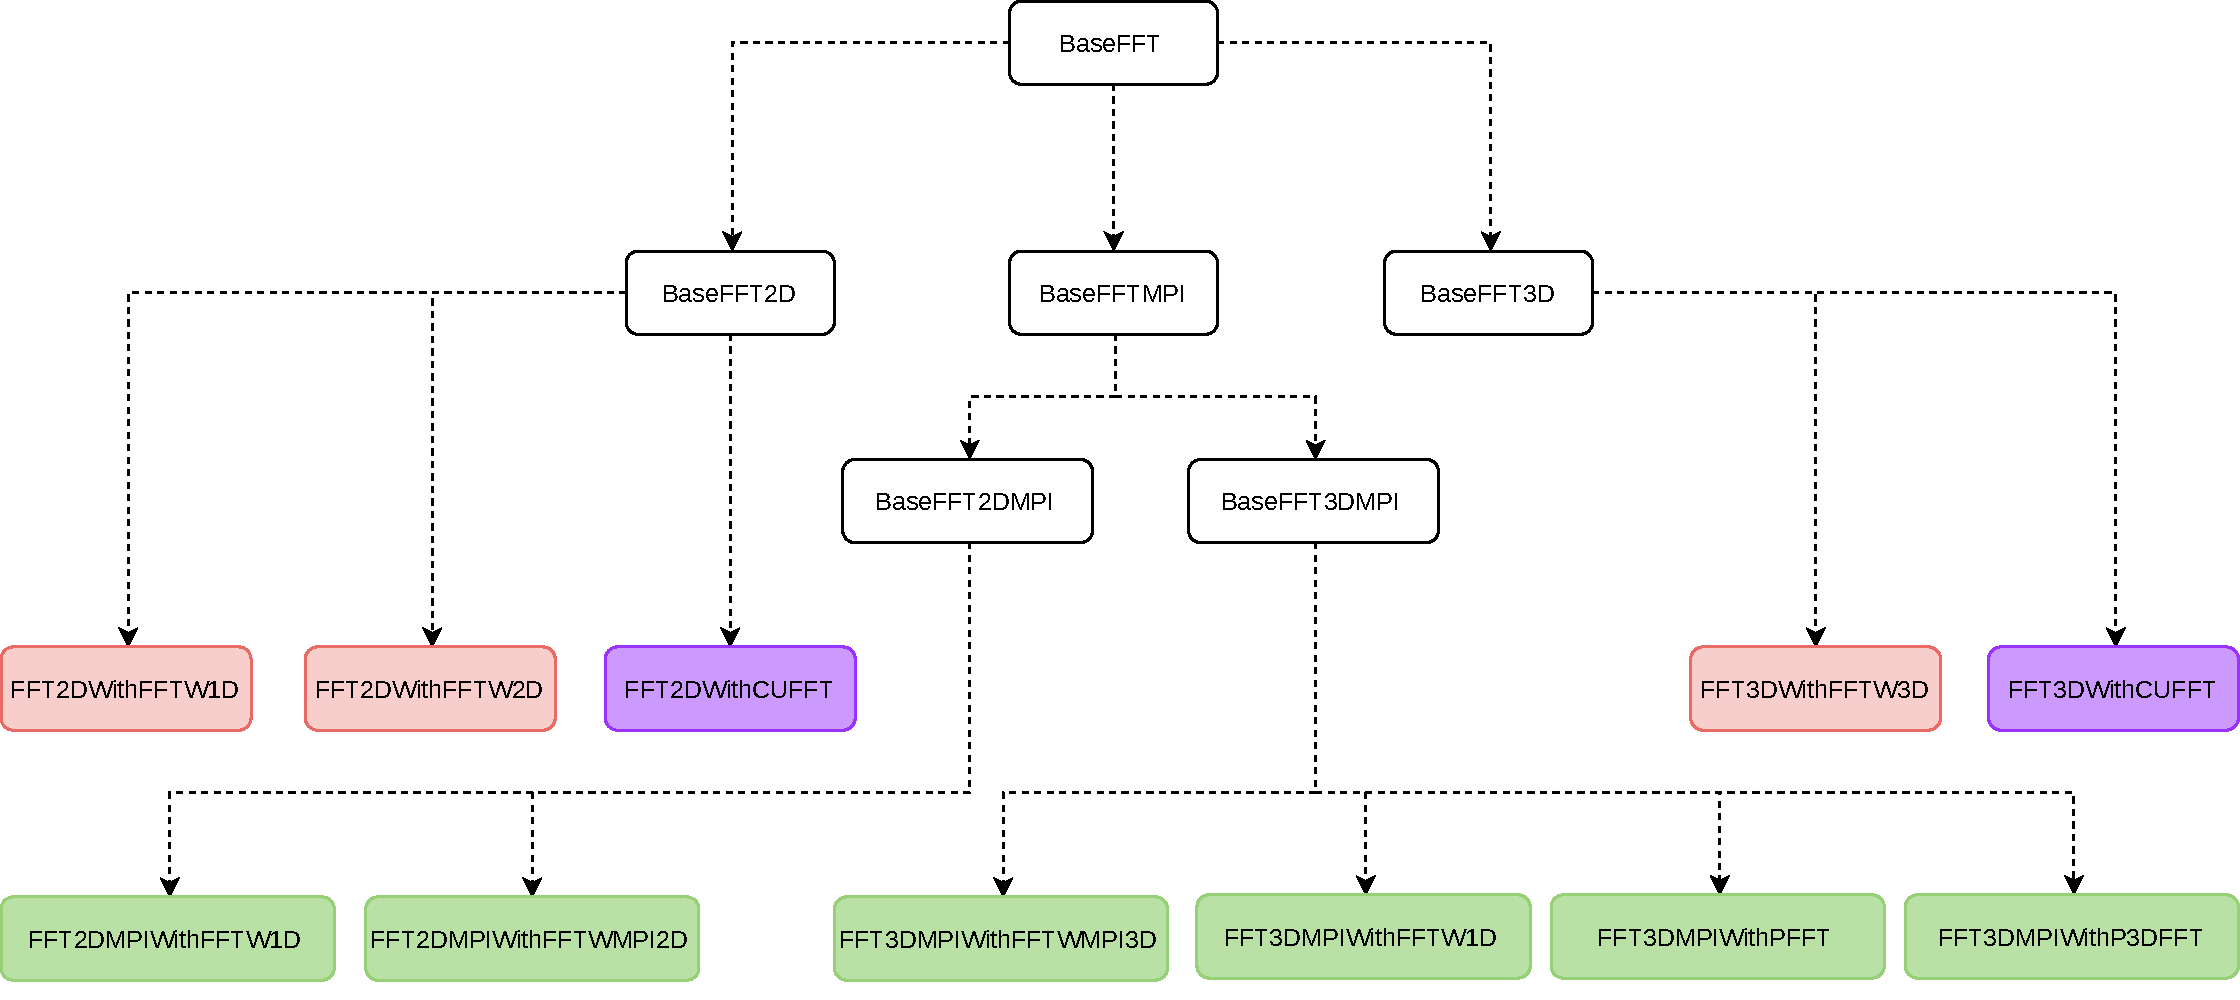
\includegraphics[width=\linewidth]{Pyfig/fig_classes}
  \caption{Class hierarchy demonstrating object-oriented approach. The
    sequential classes are shown in red, the CUDA-based classes in magenta and
    the MPI-based classes in green. The arrows represent inheritance from
    parent to child class.
  }\label{fig:classes}
\end{figure}

The C++ API is implemented as a hierarchy of classes as shown in
Fig.~\ref{fig:classes}.
%
The naming convention used for the classes (\codeinline{<Type of FFT>With<Name of
Library>}) is a cue for how these are functioning internally.
%
By utilizing inheritance, the classes share the same function names and syntax
defined in the \emph{base} classes, shown in white boxes in
Fig.~\ref{fig:classes}. Some examples of such functions are:

\begin{itemize}
  \item \codeinline{alloc\_array\_X}: Allocates array to store a physical array
    with real datatype for the current process.
  \item \codeinline{alloc\_array\_K}: Allocates array to store a spectral array
    with complex datatype  for the current process.
  \item \codeinline{init\_array\_X\_random}: Allocates and initializes a physical
    array with random values.
  \item \codeinline{test}: Run tests for a class by comparing mean and mean energy
    values in an array before and after a set of \codeinline{fft} and
    \codeinline{ifft} calls.
  \item \codeinline{bench}: Benchmark the \codeinline{fft} and
    \codeinline{ifft} methods for certain number of iterations.
\end{itemize}

Remaining methods which are specific to a library are defined in the
corresponding child classes, depicted in coloured boxes in
Fig.~\ref{fig:classes}, for example:

\begin{itemize}
  \item \codeinline{are\_parameters\_bad}: Verifies whether the global array
    shape can be decomposed with the number of MPI processes available or not.
    If the parameters are compatible, the method returns \codeinline{false}.
    This method is called prior to initializing the class.
  \item \codeinline{fft} and \codeinline{ifft}: Forward and inverse FFT
    methods.
\end{itemize}

Let us illustrate with a trivial example, wherein we initialize the FFT with a
random physical array, and perform a set of \codeinline{fft} and \codeinline{ifft}
operations.
\begin{minted}[fontsize=\footnotesize]{cpp}
#include <iostream>
using namespace std;

#include <fft3dmpi_with_fftwmpi3d.h>
// #include <fft3dmpi_with_p3dfft.h>

int main(int argc, char **argv) {
  int N0 = N1 = N2 = 32;
  // MPI-related
  int nb_procs = 4;
  MPI_Init(&argc, &argv);
  MPI_Comm_size(MPI_COMM_WORLD, &(nb_procs));

  myreal* array_X;
  mycomplex* array_K;

  FFT3DMPIWithFFTWMPI3D o(N0, N1, N2);
  // FFT3DMPIWithP3DFFT o(N0, N1, N2);

  o.init_array_X_random(array_X);
  o.alloc_array_K(array_K);
  o.fft(array_X, array_K);
  o.ifft(array_K, array_X);
  MPI_Finalize();
  return 0;
}
\end{minted}

As suggested through comments above, in order to switch the FFT library, the
user only needs to change the header file and the class name. An added
advantage is that, the user does not need to bother about the domain
decomposition while declaring and allocating the arrays. A few more helper
functions are available with the FFT classes, such as functions to compute the
mean value and energies in the array. These are demonstrated with examples in
the documentation.\footnote{%
\url{https://fluidfft.readthedocs.io/en/latest/examples/cpp.html}.}
%
Detailed information regarding the C++ classes and its member functions are
also included in the online documentation\footnote{%
\url{https://fluidfft.readthedocs.io/en/latest/doxygen/index.html}.}.

\subsection{Python API} Similar to other packages in the FluidDyn project,
\fluidpack{fft} also uses an object-oriented approach, providing FFT classes.
%
This is in contrast with the approach adopted by \pack{numpy.fft} and \pack{%
scipy.fftpack} which provides functions instead, with which the user has to
figure out the procedure to design the input values and to use the return
values, from the documentation.
%
In \fluidpack{fft}, the Python API wraps all the functionalities of its C++
counterpart and offers a richer experience through an accompanying
operator class.

As a short example, let us try to calculate the gradient of a plane sine-wave
using spectral methods, mathematically described as follows:

\begin{align*}
  u(x,y) &=
    \sin(x + y) &\forall x,y \in \left[0, L \right] \\
  \hat u(k_x,k_y) &=
    \frac{1}{L^2}
    \int_0^{L}\int_0^{L}
    u(x,y) \exp(ik_x x + ik_y y) dx dy \\
  \nabla u(x,y) &=
    \sum_{k_x} \sum_{k_y}
    i\mathbf{k}
    \hat u(k_x,k_y) \exp(-ik_x x - ik_y y)
\end{align*}
%
where $k_x$, $k_y$ represent the wavenumber corresponding to $x$ and $y$ directions,
and $\mathbf{k}$ is the wavenumber vector.

The equivalent pseudo-spectral implementation in \fluidpack{fft} is as follows:
\begin{minted}[fontsize=\footnotesize]{python}
  from fluidfft.fft2d.operators import OperatorsPseudoSpectral2D, pi
  from numpy import sin

  nx = ny = 100
  lx = ly = 2 * pi

  oper = OperatorsPseudoSpectral2D(nx, ny, lx, ly, fft="fft2d.with_fftw2d")

  u = sin(oper.XX + oper.YY)
  u_fft = oper.fft(u)
  px_u_fft, py_u_fft = oper.gradfft_from_fft(u_fft)
  px_u = oper.ifft(px_u_fft)
  py_u = oper.ifft(py_u_fft)
  grad_u = (px_u, py_u)
\end{minted}

A parallelized version of the code above will work out of the box, simply by
replacing the FFT class with an MPI-based FFT class, for instance
\codeinline{fft2d.with\_fftwmpi2d}. One can also let \fluidpack{fft} automatically
choose an appropriate FFT class by instantiating the operator class with
\codeinline{fft=None} or \codeinline{fft="default"}. Even if one finds the methods
in the operator class to be lacking, one can inherit the class and easily create a
new method, for instance using the wavenumber arrays, \codeinline{oper.KX} and
\codeinline{oper.KY}.  Arguably, a similar implementation with other available
packages would require the know-how on how FFT arrays are allocated in the memory,
normalized, decomposed in parallel and so on.
%
Moreover, the FFT and the operator classes contain objects describing the shapes
of the real and complex arrays and how the data is shared between processes.
%
A more detailed introduction on how
to use \fluidpack{fft} and available functions can be found in the
tutorials\footnote{%
\url{https://fluidfft.readthedocs.io/en/latest/tutorials.html}.}.

Thus, we have demonstrated how, by using \fluidpack{fft}, a developer can
easily switch between FFT libraries.
%
Let us now turn our attention to how the code is organized. We shall also describe
how the source code is built, and linked with the supported libraries.

\subsection{Code organization}
\begin{figure}[htp]
  \centering
  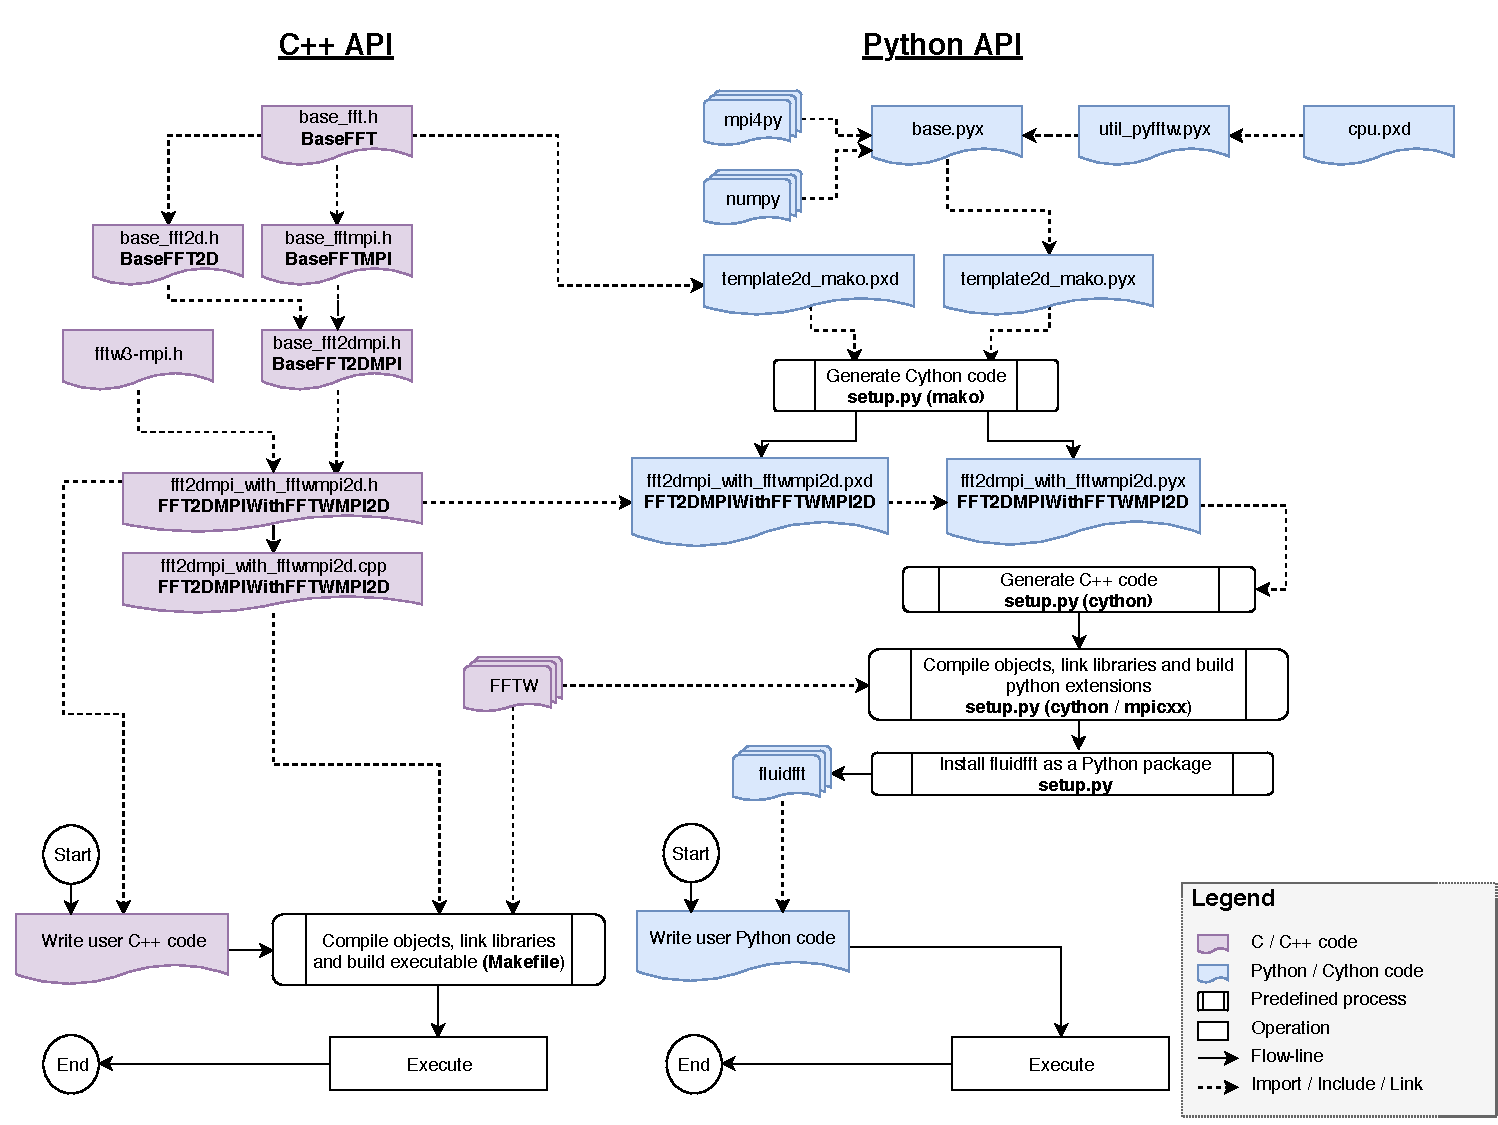
\includegraphics[width=0.96\linewidth]{Pyfig/fig_build_use}
  \caption{Flowchart illustrating how the C++ and Python API are built and used
  for one particular class, viz. \codeinline{FFT2DMPIWithFFTWMPI2D}. The dotted
  arrows in C++ part stand for include statements, demonstrating the class
  hierarchy and in the Python part indicate how different codes are imported. On
  the bottom, a smaller flowchart demonstrates how to use the API by writing user
  code.  }\label{fig:build_use}
\end{figure}

The internal architecture of \fluidpack{fft} can be visualized as layers.  Through
Fig.~\ref{fig:build_use}, we can see how these layers are linked together forming
the API for C++ and Python development. For simplicity, only one FFT class is
depicted in the figure, namely \codeinline{FFT2DMPIWithFFTWMPI2D}, which wraps
\libpack{FFTW}'s parallelized 2D FFT implementation. The C++ API is accessed by
importing the appropriate header file and building the user code with a Makefile,
an example of which is available \href{%
https://fluidfft.readthedocs.io/en/latest/examples/cpp.html}{%
in the documentation}.

The Python API is built automatically when \fluidpack{fft} is
installed\footnote{%
\href{https://fluidfft.readthedocs.io/en/latest/install.html}{Detailed steps
for installation} are provided in the documentation.}.
%
It first generates the Cython source code as a pair of \codeinline{.pyx} and
\codeinline{.pxd} files containing a class wrapping its C++
counterpart\footnote{Uses an approach similar to guidelines \href{%
    https://cython.readthedocs.io/en/latest/src/userguide/wrapping_CPlusPlus.html}{%
``Using C++ in Cython''} in the Cython documentation.}.
%
The Cython files are produced from template files (specialized for the 2D and
3D cases) using the template library \mako.
%
Thereafter, \pack{Cython} \citep{behnel_cython2011} generates C++ code with
necessary Python bindings, which are then built in the form of extensions or
dynamic libraries importable in Python code. All the built extensions are then
installed as a Python package named \fluidpack{fft}.

A helper function \codeinline{fluidfft.import\_fft\_class} is provided with the
package to simply import the FFT class. However, it is more convenient and
recommended to use an operator class, as described in the example for Python
API.\@ Although the operator classes can function as pure Python code, some of
its critical methods can be compiled, if \pack{Pythran}
\citep{guelton2018pythran} is available during installation of
\fluidpack{fft}. We will show towards the end of this section that by using
\pack{Pythran}, we reach the performance of the equivalent Fortran code.

To summarize, \fluidpack{fft} consists of the following layers:
\begin{itemize}

\item One C++ class per FFT library derived from a hierarchy of C++ classes
as shown in Fig.~\ref{fig:classes}.

\item \pack{Cython} wrappers of the C++ classes with their unit test cases.

\item Python operator classes (2D and 3D) to write code independently of the
library used for the computation of the FFT and with some mathematical helper
methods. These classes are accompanied by unit test cases.

\item \pack{Pythran} functions to speedup critical methods in the Python
operator classes.

\end{itemize}

Command-line utilities (\codeinline{fluidfft-bench} and
\codeinline{fluidfft-bench-analysis}) are also provided with the \fluidpack{fft}
installation to run benchmarks and plot the results. In the next subsection, we
shall look at some results by making use of these utilities on three computing
clusters.

\subsection{Performance}

\paragraphbf{Scalability tests using \codeinline{fluidfft-bench}}

% Simple!! Few cases. Few clusters. Figures obtained with
% fluidfft-bench-analysis

Scalability of \fluidpack{fft} is measured in the form of strong scaling speedup,
defined in the present context as:
\begin{equation*}
S_\alpha(n_p) = \frac
{[\mathrm{Time\ elapsed\ for\ } N \mathrm{\ iterations\ with\ }n_{p,\min}\mathrm{\ processes}]_{\mathrm{fastest}}
\times n_{p,\min}}
{[\mathrm{Time\ elapsed\ for\ } N \mathrm{\ iterations\ with\ } n_p \mathrm{\
processes}]_\alpha}
\label{eq:speedup}
\end{equation*}

where $n_{p,\min}$ is the minimum number of processes employed for a specific
array size and hardware. The subscripts, $\alpha$ denotes the FFT class used and
``fastest'' corresponds to the fastest result among various FFT classes.

To compute strong scaling the utility \codeinline{fluidfft-bench} is launched
as scheduled jobs on HPC clusters, ensuring no interference from background
processes. No hyperthreading was used.
%
We have used $N=20$ iterations for each run, with which we obtain sufficiently
repeatable results.
%
For a particular choice of array size, every FFT class available are
benchmarked for the two tasks, forward and inverse FFT. Three different function
variants are compared (see the legend in subsequent figures):

\begin{itemize}

\item \codeinline{fft\_cpp}, \codeinline{ifft\_cpp} (continuous lines): benchmark
of the C++ function from the C++ code. An array is passed as an argument to store
the result. No memory allocation is performed inside these functions.

\item \codeinline{fft\_as\_arg}, \codeinline{ifft\_as\_arg} (dashed lines):
benchmark of a Python method from Python. Similar to the C++ code, the second
argument of this method is an array to contain the result of the transform, so no
memory allocation is needed.

\item \codeinline{fft\_return}, \codeinline{ifft\_return} (dotted lines):
benchmark of a Python method from Python. No array is provided to the function to
contain the result, and therefore a numpy array is created and then returned by
the function.

\end{itemize}

On big HPC clusters, we have only focussed on 3D array transforms as benchmark
problems, since these are notoriously expensive to compute and require massive
parallelization.  The physical arrays used in all four 3D MPI based FFT classes
are identical in structure.  However, there are subtle differences, in terms of
how the domain decomposition and the allocation of the transformed array in the
memory are handled\footnote{Detailed discussion on \href{%
https://fluidfft.readthedocs.io/en/latest/ipynb/executed/tuto_fft3d_mpi_domain_decomp.html}{%
``FFT 3D parallel (MPI): Domain decomposition''} tutorial}.

Hereafter, for the sake of brevity, the FFT classes will be named in terms of the
associated library (For example, the class \codeinline{FFT3DMPIWithFFTW1D} is
named \codeinline{fftw1d}).  Let us go through the results\footnote{Saved at
\url{%
https://bitbucket.org/fluiddyn/fluidfft-bench-results}} plotted using
\codeinline{fluidfft-bench-analysis}.

\paragraph{Benchmarks on Occigen}

\href{https://www.top500.org/system/178465}{Occigen} is a GENCI-CINES HPC
cluster which uses Intel Xeon CPU E5--2690 v3 (2.6 GHz) processors with 24 cores
per node. The installation was performed using Intel C++ 17.2 compiler, Python
3.6.5, and OpenMPI 2.0.2.

\begin{figure}[htp!]
\centering
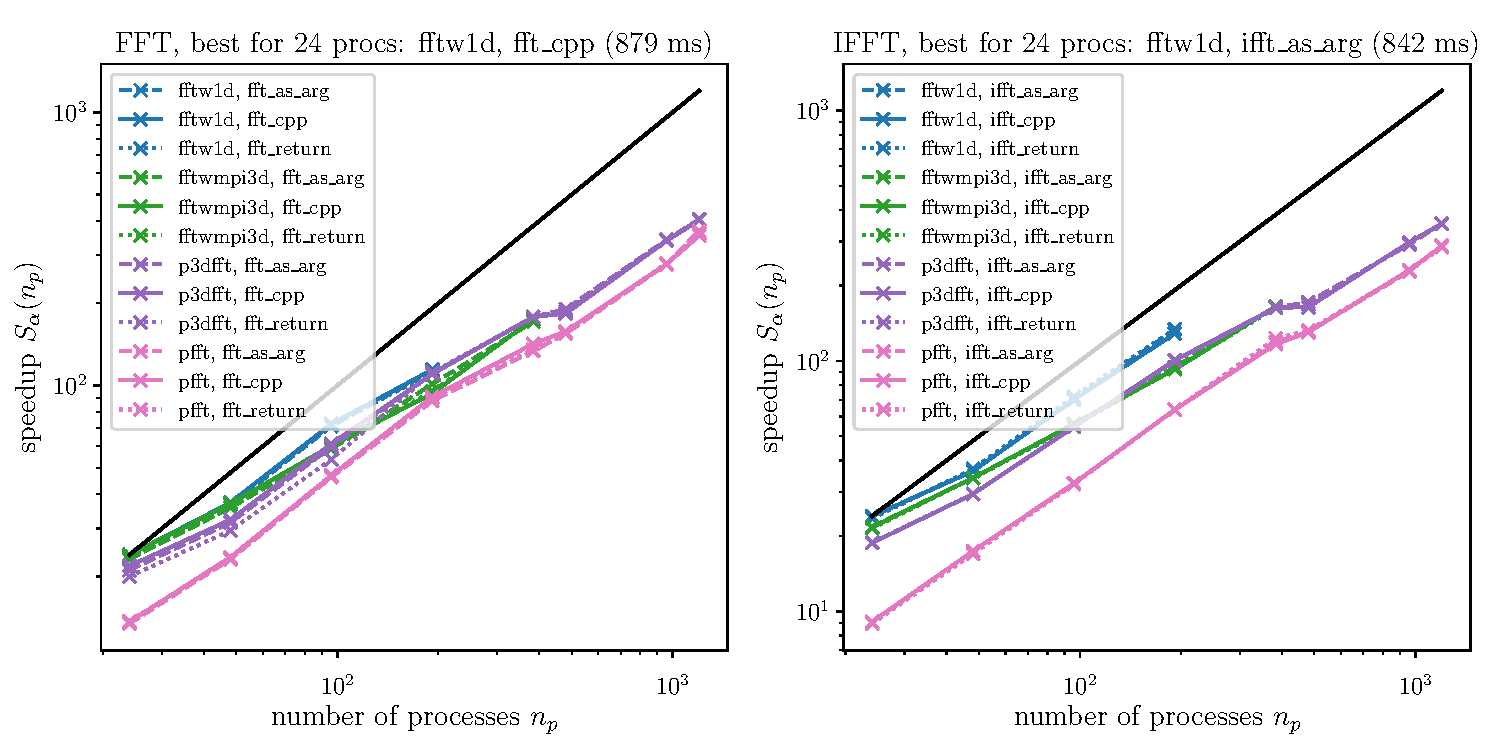
\includegraphics[width=\linewidth]{tmp/fig_occigen_384x1152x1152}
\caption{Speedup computed from the median of the elapsed times for 3D fft
(384$\times$1152$\times$1152, left: fft and right: ifft) on Occigen.}%
\label{fig:occigen384x1152x1152}
\end{figure}

Fig.~\ref{fig:occigen384x1152x1152} demonstrates the strong scaling performance
of a cuboid array sized $384\times1152\times1152$. This case is particularly
interesting since for FFT classes implementing 1D domain decomposition
(\codeinline{fftw1d} and \codeinline{fftwmpi3d}), the processes are spread on
the first index for the physical input array. This restriction is as a result
of some \libpack{FFTW} library internals and design choices adopted in
\fluidpack{fft}. This limits \codeinline{fftw1d} (our own MPI implementation
using MPI types and 1D transforms from FFTW) to 192 cores and
\codeinline{fftwmpi3d} to 384 cores. The latter can utilize more cores since it
is capable of working with empty arrays, while sharing some of the
computational load.
%
The fastest methods for relatively
low and high number of processes are \codeinline{fftw1d} and
\codeinline{p3dfft} respectively for the present case.

The benchmark is not sufficiently accurate to measure the cost of calling the
functions from Python (difference between continuous and dashed lines,
i.e. between pure C++ and the \codeinline{as\_arg} Python method) and even the
creation of the numpy array (difference between the dashed and the dotted line,
i.e. between the \codeinline{as\_arg} and the \codeinline{return} Python
methods).


\begin{figure}[htp!]
\centering
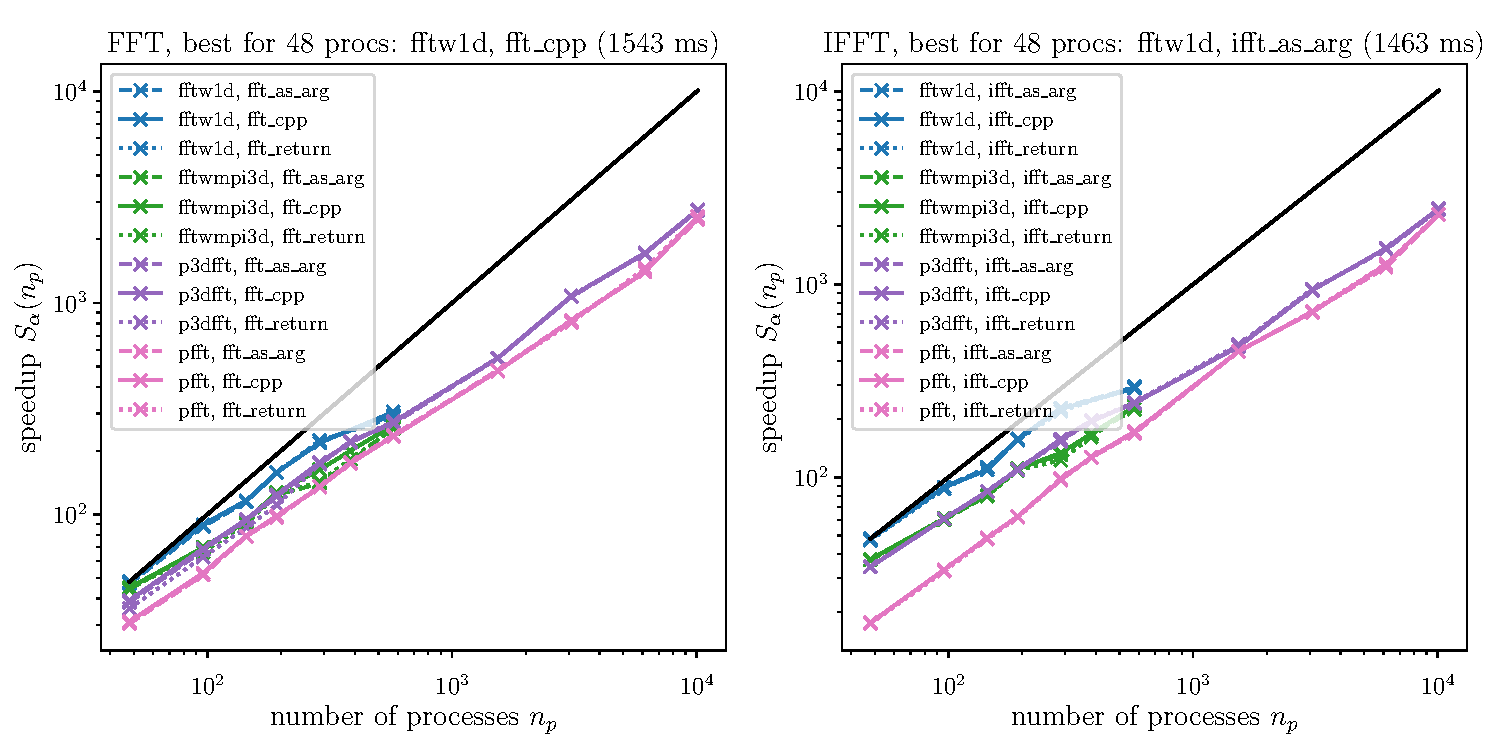
\includegraphics[width=\linewidth]{tmp/fig_occigen_1152x1152x1152}
\caption{Speedup computed from the median of the elapsed times for 3D fft
(1152$\times$1152$\times$1152, left: fft and right: ifft) on Occigen.}
\label{fig:occigen1152x1152x1152}
\end{figure}

Fig.~\ref{fig:occigen1152x1152x1152} demonstrates the strong scaling
performance of a cubical array sized $1152\times1152\times1152$. For this
resolution as well, \codeinline{fftw1d} is the fastest method when using only
few cores and it can not be used for more that 192 cores. The faster library
when using more cores is also \codeinline{p3dfft}. This also shows that
\fluidpack{fft} can effectively scale for over 10,000 cores with a significant
increase in speedup.


\paragraph{Benchmarks on Beskow}

\href{ https://www.pdc.kth.se/hpc-services/computing-systems}{Beskow} is a Cray
machine maintained by SNIC at PDC, Stockholm. It runs on Intel(R) Xeon(R) CPU
E5-2695 v4 (2.1 GHz) processors with 36 cores per node. The installation was
done using Intel C++ 18 compiler, Python 3.6.5 and CRAY-MPICH 7.0.4.

\begin{figure}[htp!]
\centering
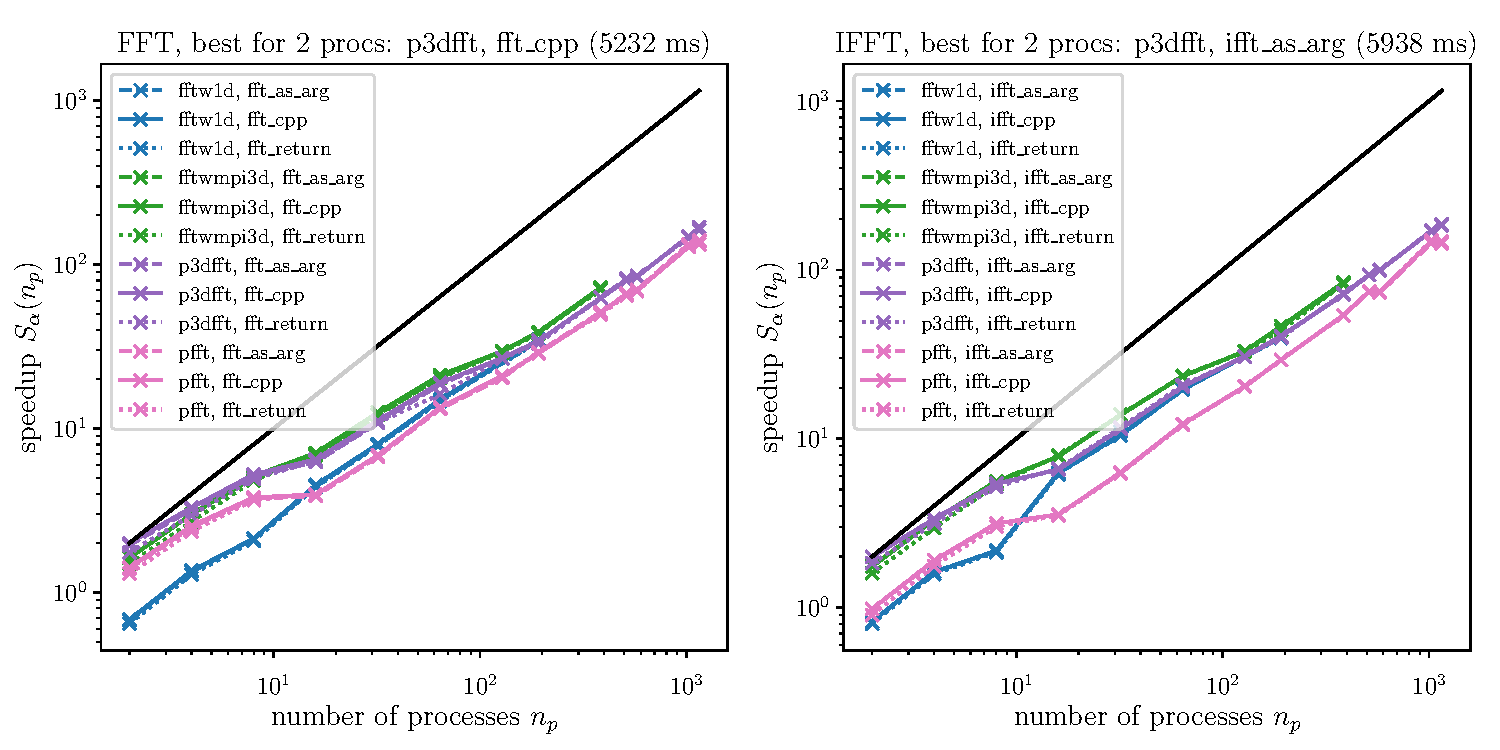
\includegraphics[width=\linewidth]{tmp/fig_beskow_384x1152x1152}
\caption{Speedup computed from the median of the elapsed times for 3D fft
(384$\times$1152$\times$1152, left: fft and right: ifft) on Beskow.}
\label{fig:beskow384x1152x1152}
\end{figure}

In Fig.~\ref{fig:beskow384x1152x1152}, the strong scaling results of the cuboid
array can be observed. In this set of results we have also included intra-node
scaling, wherein there is no latency introduced due to typically slower
node-to-node communication. The fastest library for very low (below 16) and
very high (above 384) number of processes in this configuration is
\codeinline{p3dfft}. For moderately high number of processes (16 and above) the
fastest library is \codeinline{fftwmpi3d}. Here too, we notice that
\codeinline{fftw1d} is limited to 192 cores and \codeinline{fftwmpi3d} to 384
cores, for reasons mentioned earlier.

A striking difference when compared with Fig.~\ref{fig:occigen384x1152x1152} is
that \codeinline{fftw1d} is not the fastest of the four classes in this machine.
One can only speculate that this could be a consequence of the differences in MPI
library and hardware which has been employed. This also emphasises the need to
perform benchmarks when using an entirely new configuration.

\begin{figure}[htp!]
\centering
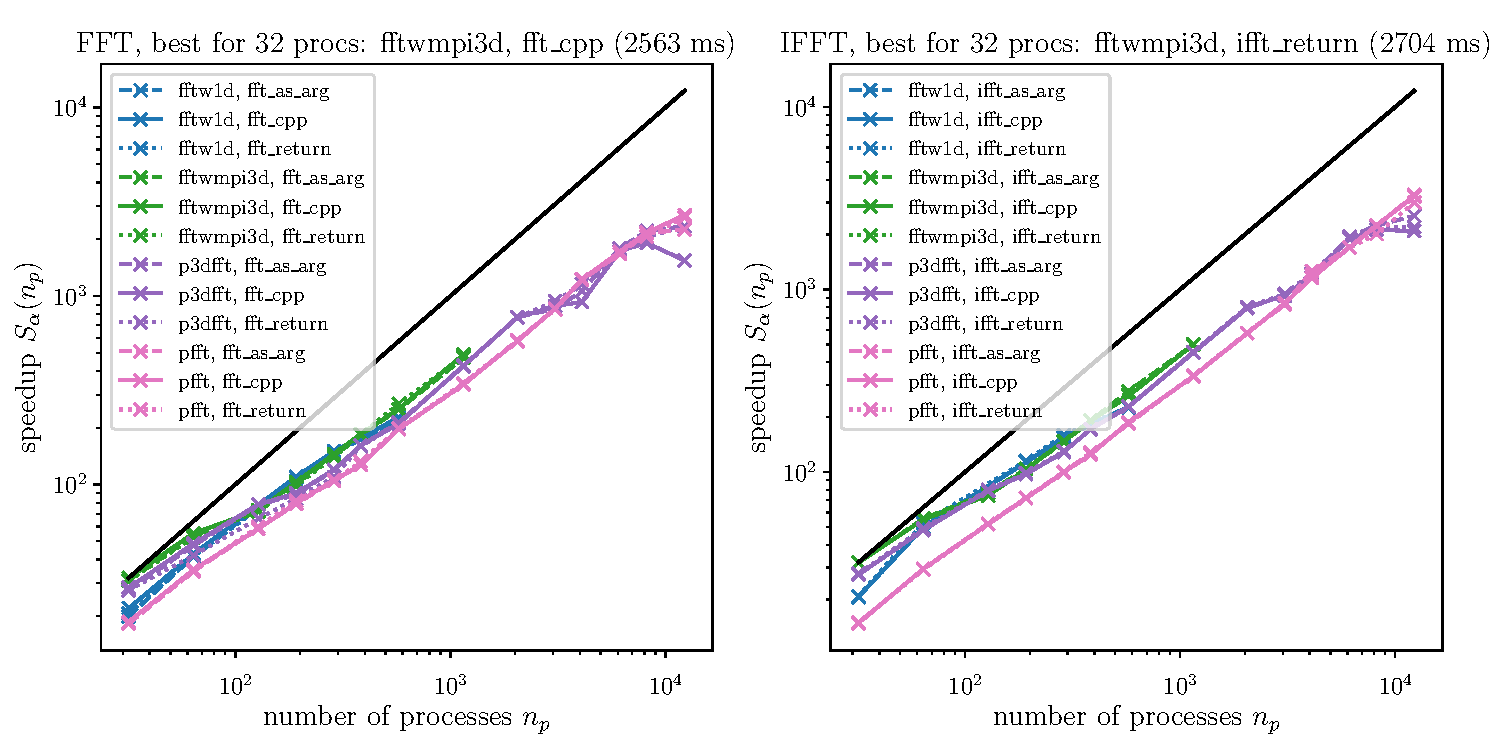
\includegraphics[width=\linewidth]{tmp/fig_beskow_1152x1152x1152}
\caption{Speedup computed from the median of the elapsed times for 3D fft
(1152$\times$1152$\times$1152, left: fft and right: ifft) on Beskow.}
\label{fig:beskow1152x1152x1152}
\end{figure}

The strong scaling results of the cubical array on Beskow are displayed on
Fig.~\ref{fig:beskow1152x1152x1152}, wherein we restrict to inter-node
computation.  We observe that the fastest method for low number of processes is
again, \codeinline{fftwmpi3d}. When high number of processes (above 1000)
are utilized, initially \codeinline{p3dfft} is the faster methods as before,
but with 3000 and above processes, \codeinline{pfft} is comparable in speed and
sometimes faster.

\paragraph{Benchmarks on a LEGI cluster}

Let us also analyse how \fluidpack{fft} scales on a computing cluster
maintained at an institutional level, named Cluster8 at \href{%
http://www.legi.grenoble-inp.fr}{LEGI}, Grenoble. This cluster functions using
Intel Xeon CPU E5-2650 v3 (2.3 GHz) with 20 cores per node and \fluidpack{fft}
was installed using a toolchain which comprises of gcc 4.9.2, Python 3.6.4 and
OpenMPI 1.6.5 as key software components.

\begin{figure}[htp!]
\centering
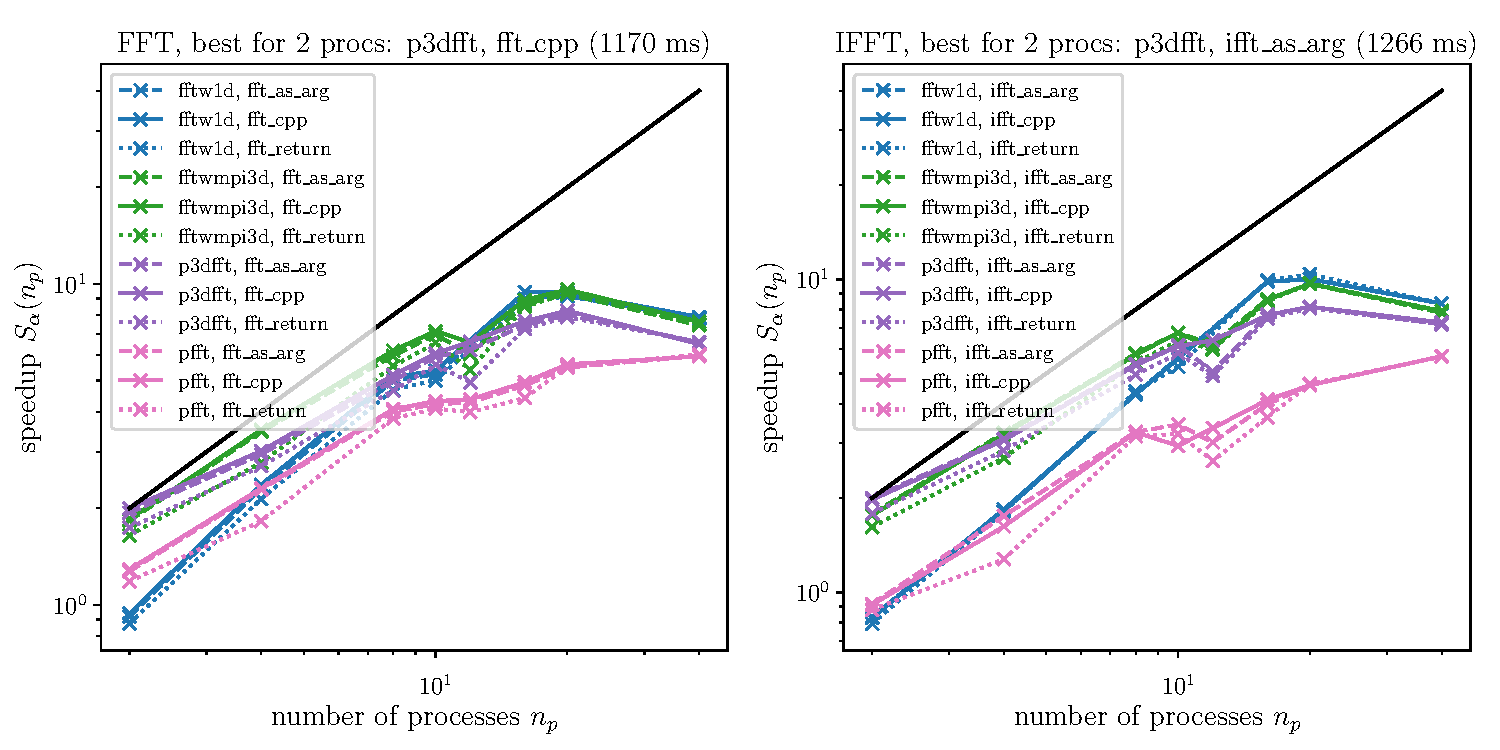
\includegraphics[width=\linewidth]{tmp/fig_legi_cluster8_320x640x640}
\caption{Speedup computed from the median of the elapsed times for 3D fft
(320$\times$640$\times$640) at LEGI on cluster8.}
\label{fig:cluster8:320x640x640}
\end{figure}

In Fig.~\ref{fig:cluster8:320x640x640} we observe that the strong scaling for an
array shape of $320\times640\times640$ is not far from the ideal linear trend. The
fastest library is \codeinline{fftwmpi3d} for this case.  As expected from FFT
algorithms, there is a slight drop in speedup when the array size is not exactly
divisible by the number of processes, i.e.\ with 12 processes. The speedup
declines rapidly when more than one node is employed (above 20 processes). This
effect can be attributed to the latency introduced by inter-node communications, a
hardware limitation of this cluster (10 Gb/s).

\begin{figure}[htp!]
\centering
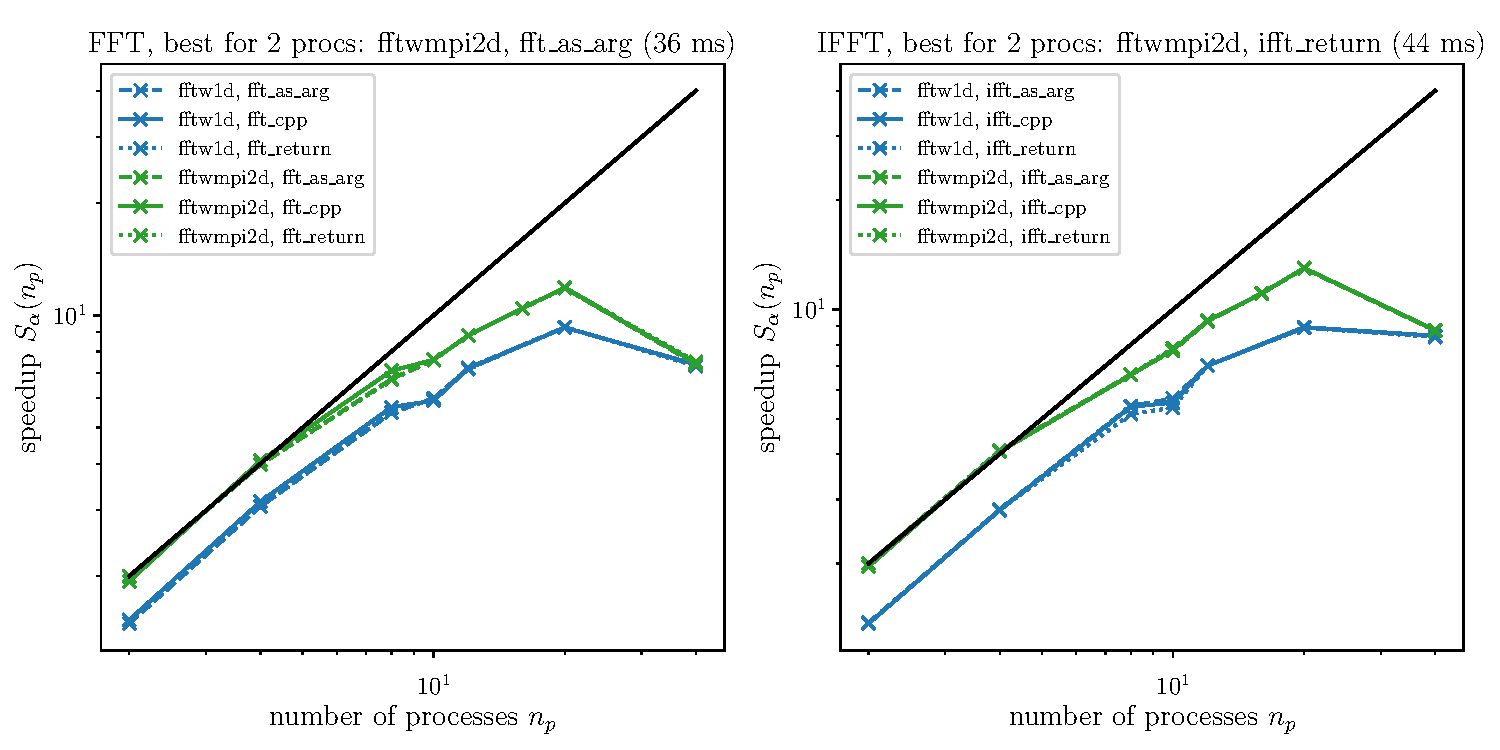
\includegraphics[width=\linewidth]{tmp/fig_legi_cluster8_2160x2160}
\caption{Speedup computed from the median of the elapsed times for 2D fft
(2160$\times$2160) at LEGI on cluster8.}
\label{fig:cluster8:2160x2160}
\end{figure}

We have also analysed the performance of 2D MPI enabled FFT classes on the same
machine using an array shaped $2160\times2160$ in
Fig.~\ref{fig:cluster8:2160x2160}. The fastest library is
\codeinline{fftwmpi2d}. Both \codeinline{fftw1d} and \codeinline{fftwmpi2d}
libraries display near-linear scaling, except when more than one node is used
and the performance tapers off.

As a conclusive remark on scalability, a general rule of thumb should be to use
1D domain decomposition when only very few processors are employed. For massive
parallelization, 2D decomposition is required to achieve good speedup without
being limited by the number of processors at disposal. We have thus shown that
overall performance of the libraries interfaced by \fluidpack{fft} are quite
good, and there is no noticeable drop in speedup when the Python API is used.
%
This benchmark analysis also shows that the fastest FFT implementation depends
on the size of the arrays and on the hardware.
%
Therefore, an application build upon \fluidpack{fft} can be efficient for
different sizes and machines.


\paragraphbf{Microbenchmark of critical ``operator'' functions}

As already mentioned, we use \pack{Pythran} \citep{guelton2018pythran} to
compile some critical ``operator'' functions.  In this subsection, we present a
microbenchmark for one simple task used in pseudo-spectral codes: projecting a
velocity field on a non-divergent velocity field.  It is performed in spectral
space, where it can simply be written as
\begin{minted}[fontsize=\footnotesize]{python}
# pythran export proj_out_of_place(
#     complex128[][][], complex128[][][], complex128[][][],
#     float64[][][], float64[][][], float64[][][], float64[][][])

def proj_out_of_place(vx, vy, vz, kx, ky, kz, inv_k_square_nozero):
    tmp = (kx * vx + ky * vy + kz * vz) * inv_k_square_nozero
    return vx - kx * tmp, vy - ky * tmp, vz - kz * tmp
\end{minted}
Note that, this implementation is ``out-of-place'', meaning that the result is
returned by the function and that the input velocity field (\codeinline{vx, vy,
vz}) is unmodified.
%
The comment above the function definition is a \pack{Pythran} annotation, which
serves as a type-hint for the variables used within the functions --- all
arguments being \pack{Numpy} arrays in this case.
%
\pack{Pythran} needs such annotation to be able to compile this code into
efficient machine instructions \emph{via} a C++ code.
%
Without \pack{Pythran} the annotation has no effect, and
of course, the function defaults to using Python with \pack{Numpy} to execute.

The array notation is well adapted and less verbose to express this simple
vector calculus.
%
Since explicit loops with indexing is not required, the computation with Python
and \pack{Numpy} is not extremely slow. Despite this being quite a favourable
case for \pack{Numpy}, the computation with \pack{Numpy} is not optimized
because, internally, it involves many loops (one per arithmetic operator) and
creation of temporary arrays.
%av: Have I understood correctly here with the clarifications: "internally" &
%   "arithmetic operator"?

\begin{figure}[htp]
\centering
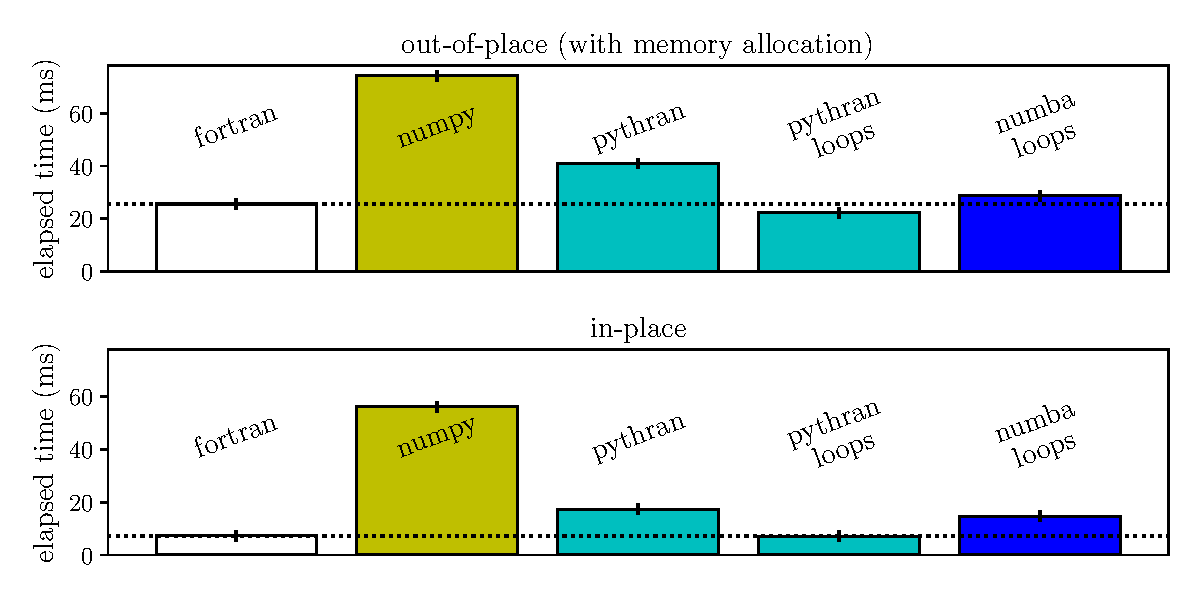
\includegraphics[width=\linewidth]{tmp/fig_microbench}
\caption{Elapsed time (smaller is better) for the projection function for
different implementations and tools.  The shape of the arrays is
$(128,\ 128,\ 65)$. The dotted lines indicate the times for Fortran for better
comparison.}
\label{fig:microbench}
\end{figure}

In the top axis of Fig.~\ref{fig:microbench}, we compare the elapsed times for
different implementations of this function.
%
For this out-of-place version, we used three different codes:
\begin{enumerate}
\item a Fortran code (not shown\footnote{The codes and a Makefile used for this
benchmark study are available in \href{%
https://bitbucket.org/fluiddyn/fluiddyn_paper/src/default/fluidfft/microbench/}{%
the repository of the article}.}) written with three nested explicit loops (one
per dimension). Note that as in the Python version we also allocate the memory
where the result is stored.
\item the simplest Python version shown above.
\item a Python version with three nested explicit loops:
% (code not shown).
\begin{minted}[fontsize=\footnotesize]{python}
# pythran export proj_out_of_place_loop(
#     complex128[][][], complex128[][][], complex128[][][],
#     float64[][][], float64[][][], float64[][][], float64[][][])

def proj_out_of_place_loop(vx, vy, vz, kx, ky, kz, inv_k_square_nozero):

    rx = np.empty_like(vx)
    ry = np.empty_like(vx)
    rz = np.empty_like(vx)

    n0, n1, n2 = kx.shape

    for i0 in range(n0):
        for i1 in range(n1):
            for i2 in range(n2):
                tmp = (kx[i0, i1, i2] * vx[i0, i1, i2]
                       + ky[i0, i1, i2] * vy[i0, i1, i2]
                       + kz[i0, i1, i2] * vz[i0, i1, i2]
                ) * inv_k_square_nozero[i0, i1, i2]

                rx[i0, i1, i2] = vx[i0, i1, i2] - kx[i0, i1, i2] * tmp
                ry[i0, i1, i2] = vz[i0, i1, i2] - kx[i0, i1, i2] * tmp
                rz[i0, i1, i2] = vy[i0, i1, i2] - kx[i0, i1, i2] * tmp

    return rx, ry, rz
\end{minted}
\end{enumerate}
For the version without explicit loops, we present the elapsed time for two
cases: (i) simply using Python (yellow bar) and (ii) using the Pythranized
function (first cyan bar).
%
For the Python version with explicit loops, we only present the results for (i)
the Pythranized function (second cyan bar) and (ii) the result of \pack{Numba}
(blue bar).
%
We do not show the result for \pack{Numba} for the code without explicit loops
because it is slower than \pack{Numpy}. We have also omitted the result for
\pack{Numpy} for the code with explicit loops because it is very inefficient.
%
The timing is performed upon tuning the computer using the package
\href{https://pypi.org/project/perf/}{\pack{perf}}.

We see that \pack{Numpy} is approximately three time slower than the Fortran
implementation (which as already mentioned contains the memory allocation).
%
Just using \pack{Pythran} without changing the code (first cyan bar), we save
nearly 50\% of the execution time but we are still significantly slower than
the Fortran implementation.
%
We reach the Fortran performance (even slightly faster) only by using
\pack{Pythran} with the code with explicit loops.
%
With this code, \pack{Numba} is nearly as fast (but still slower) without
requiring any type annotation.

Note that the exact performance differences depend on the hardware, the software
versions\footnote{Here, we use Python~3.6.4 (packaged by conda-forge),
\pack{Numpy}~1.13.3, \pack{Pythran}~0.8.5, \pack{Numba}~0.38, gfortran~6.3 and
clang~6.0.}, the compilers and the compilation options.
%
We use \codeinline{gfortran -O3 -march=native} for Fortran and
\codeinline{clang++ -O3 -march=native} for \pack{Pythran}\footnote{The results
with \codeinline{g++ -O3 -march=native} are very similar but tend to be slightly
slower.}.
%


Since allocating memory is expensive and we do not need the non-projected
velocity field after the call of the function, an evident optimization is to
put the output in the input arrays.  Such an ``in-place'' version can be written
with \pack{Numpy} as:
\begin{minted}[fontsize=\footnotesize]{python}
# pythran export proj_in_place(
#     complex128[][][], complex128[][][], complex128[][][],
#     float64[][][], float64[][][], float64[][][], float64[][][])

def proj_in_place(vx, vy, vz, kx, ky, kz, inv_k_square_nozero):
    tmp = (kx * vx + ky * vy + kz * vz) * inv_k_square_nozero
    vx -= kx * tmp
    vy -= ky * tmp
    vz -= kz * tmp
\end{minted}

As in the first version, we have included the \pack{Pythran} annotation.
%
We also consider an ``in-place'' version with explicit loops:
\begin{minted}[fontsize=\footnotesize]{python}
# pythran export proj_in_place_loop(
#     complex128[][][], complex128[][][], complex128[][][],
#     float64[][][], float64[][][], float64[][][], float64[][][])

def proj_in_place_loop(vx, vy, vz, kx, ky, kz, inv_k_square_nozero):

    n0, n1, n2 = kx.shape

    for i0 in range(n0):
        for i1 in range(n1):
            for i2 in range(n2):
                tmp = (kx[i0, i1, i2] * vx[i0, i1, i2]
                       + ky[i0, i1, i2] * vy[i0, i1, i2]
                       + kz[i0, i1, i2] * vz[i0, i1, i2]
                ) * inv_k_square_nozero[i0, i1, i2]

                vx[i0, i1, i2] -= kx[i0, i1, i2] * tmp
                vy[i0, i1, i2] -= ky[i0, i1, i2] * tmp
                vz[i0, i1, i2] -= kz[i0, i1, i2] * tmp

\end{minted}
Note that this code is much longer and clearly less readable than the version
without explicit loops.  This is however the version which is used in
\pack{fluidfft} since it leads to faster execution.

The elapsed time for these in-place versions and for an equivalent Fortran
implementation are displayed in the bottom axis of Fig.~\ref{fig:microbench}.
%
The ranking is the same as for the out-of-place versions and \pack{Pythran} is also
the faster solution.
%
However, \pack{Numpy} is even more slower (7.8 times slower than \pack{Pythran}
with the explicit loops) than for the out-of-place versions.

From this short and simple microbenchmark, we can infer four main points:
\begin{itemize}
\item Memory allocation takes time!  In Python, memory management is automatic
and we tend to forget it.  An important rule to write efficient code is to
reuse the buffers already allocated as much as possible.

\item Even for this very simple case quite favorable for \pack{Numpy} (no indexing
or slicing), \pack{Numpy} is three to eight time slower than the Fortran
implementations. As long as the execution time is small or that the
function represents a small part of the total execution time, this is not an
issue. However, in other cases, Python-\pack{Numpy} users need to consider
other solutions.

\item \pack{Pythran} is able to speedup the \pack{Numpy} code without explicit
loops and is as fast as Fortran (even slightly faster in our case) for the
codes with explicit loops.

\item \pack{Numba} is unable to speedup the \pack{Numpy} code.
%
It gives very interesting performance for the version with explicit loops
without any type annotation but the result is significantly slower than with
\pack{Pythran} and Fortran.
\end{itemize}

For the aforementioned reasons, we have preferred \pack{Pythran} to compile
optimized ``operator'' functions that complement the FFT classes. Although with
this we obtain remarkable performance, there is still room for some
improvement, in terms of logical implementation and allocation of arrays. For
example, applications such as CFD simulations often deals with non-linear terms
which require dealiasing. The FFT classes of \fluidpack{fft}, currently
allocates the same number of modes in the spectral array so as to transform the
physical array. Thereafter, we apply dealiasing by setting zeros to wavenumbers
which are larger than, say, two-thirds of the maximum wavenumber. Instead, we
could take into account dealiasing in the FFT classes to save some memory and
computation time\footnote{See
\href{https://bitbucket.org/fluiddyn/fluidfft/issues/21/}{fluidfft issue 21}.}.

\section{Quality control}

% \textcolor{blue}{Detail the level of testing that has been carried out on the
% code (e.g. unit, functional, load etc.), and in which environments. If not
% already included in the software documentation, provide details of how a user
% could quickly understand if the software is working (e.g. providing examples of
% running the software with sample input and output data). }

The package \fluidpack{fft} currently supplies unit tests covering 90\% of its
code.  These unit tests are run regularly through continuous integration on Travis
CI with the most recent releases of \fluidpack{fft}'s dependencies and on
Bitbucket Pipelines inside a static
\href{https://hub.docker.com/u/fluiddyn}{Docker container}.  The tests are run
using standard Python interpreter with all supported versions.

For \fluidpack{fft}, the code coverage results are displayed at
\href{https://codecov.io/bb/fluiddyn/fluidfft}{Codecov}.  Using third-party
packages \pack{coverage} and \pack{tox}, it is straightforward to bootstrap the
installation with dependencies, test with multiple Python versions and combine the
code coverage report, ready for upload. It is also possible to run similar
isolated tests using \pack{tox} or coverage analysis using \pack{coverage} in a
local machine.  Up-to-date build status and coverage status are displayed on the
landing page of the Bitbucket repository.  Instructions on how to run unit tests,
coverage and lint tests are included in the documentation.

We also try to follow a consistent code style as recommended by PEP (Python
enhancement proposals) 8 and 257. This is also inspected using lint checkers such
as \codeinline{flake8} and \codeinline{pylint} among the developers.  The Python
code is regularly cleaned up using the code formatter \codeinline{black}.


\section{(2) Availability}
\vspace{0.5cm}
\section{Operating system}

% \textcolor{blue}{Please include minimum version compatibility.}

Windows and any POSIX based OS, such as GNU/Linux and macOS.

\section{Programming language}

% \textcolor{blue}{Please include minimum version compatibility.}

Python 2.7, 3.5 or above. For the next versions, we will
\href{https://python3statement.org/}{drop Python 2.7 support and Python $>=$
3.6 will be required}.
%
Note that while Cython and Pythran both use the C API of CPython, \fluidpack{fft}
has been successfully tested on PyPy 6.0.
%
A C++11 supporting compiler, while not mandatory for the C++ API or Cython
extensions of \fluidpack{fft}, is recommended to be able to use Pythran extensions.

\section{Dependencies}

% \textcolor{blue}{E.g. libraries, frameworks, incl. minimum version
% compatibility.}
C++ API:
\begin{itemize}
  \item{\bf Optional:} \pack{OpenMPI} or equivalent, \libpack{FFTW},
    \libpack{P3DFFT}, \libpack{PFFT} and \libpack{cuFFT} libraries.
\end{itemize}

Python API:

\begin{itemize}
\item {\bf Minimum:} \fluidpack{dyn}, \pack{Numpy}, \pack{Cython}, and
  \pack{mako}\ or \pack{Jinja2}; \libpack{FFTW} library.
\item {\bf Optional:} \pack{mpi4py} and \pack{Pythran}; \libpack{P3DFFT},
  \libpack{PFFT} and \libpack{cuFFT} libraries.
\end{itemize}


\section{List of contributors}

% \textcolor{blue}{Please list anyone who helped to create the software (who may
% also not be an author of this paper), including their roles and affiliations.}

\begin{itemize}
\item Pierre Augier (LEGI): creator of the FluidDyn project and of
\fluidpack{fft}.
\item Cyrille Bonamy (LEGI): C++ code and some methods in the operator classes.
\item Ashwin Vishnu Mohanan (KTH): command lines utilities, benchmarks, unit
  tests, continuous integration, and bug fixes.
\end{itemize}

\section{Software location:}

% {\bf Archive} \textcolor{blue}{(e.g. institutional repository, general
% repository) (required – please see instructions on journal website for
% depositing archive copy of software in a suitable repository)}

\begin{description}[noitemsep,topsep=0pt]
\item[Name:] PyPI
\item[Persistent identifier:] https://pypi.org/project/fluidfft
\item[Licence:] CeCILL, a free software license adapted to both international
and French legal matters, in the spirit of and retaining compatibility with the
GNU General Public License (GPL).
\item[Publisher:] Pierre Augier
\item[Version published:] 0.2.4
\item[Date published:] 02/07/2018
\end{description}

{\bf Code repository}

\begin{description}[noitemsep,topsep=0pt]
\item[Name:] Bitbucket
\item[Persistent identifier:] https://bitbucket.org/fluiddyn/fluidfft
\item[Licence:] CeCILL
\item[Date published:] 2017
\end{description}

{\bf Emulation environment}

\begin{description}[noitemsep,topsep=0pt]
\item[Name:] Docker
\item[Persistent identifier:] https://hub.docker.com/r/fluiddyn/python3-stable
\item[Licence:] CeCILL-B, a BSD compatible French licence.
\item[Date published:] 02/10/2017
\end{description}

\section{Language}

% \textcolor{blue}{Language of repository, software and supporting files.}

English

\section{(3) Reuse potential}

% \textcolor{blue}{Please describe in as much detail as possible the ways in
% which the software could be reused by other researchers both within and outside
% of your field. This should include the use cases for the software, and also
% details of how the software might be modified or extended (including how
% contributors should contact you) if appropriate. Also you must include details
% of what support mechanisms are in place for this software (even if there is no
% support).}

\fluidpack{fft} is used by the Computational Fluid Mechanics framework
\fluidpack{sim} \citep{fluidsim}. It could be used by any C++ or Python project
where real-to-complex 2D or 3D FFTs are performed.

There is no formal support mechanism. However, bug reports can be submitted at
the \href{https://bitbucket.org/fluiddyn/fluidsim/issues}{Issues page on
Bitbucket}. Discussions and questions can be aired on instant messaging
channels in Riot (or equivalent with Matrix protocol)\footnote{
\url{%
  https://matrix.to/\#/\#fluiddyn-users:matrix.org}}
or via IRC protocol on Freenode at \codeinline{\#fluiddyn-users}. Discussions
can also be exchanged via the official mailing list\footnote{
\url{https://www.freelists.org/list/fluiddyn}}.

\section{Acknowledgements}

% \textcolor{blue}{Please add any relevant acknowledgements to anyone else who
% supported the project in which the software was created, but did not work
% directly on the software itself.}

Ashwin Vishnu Mohanan could not have been as involved in this project without the
kindness of Erik Lindborg.
%
We are grateful to Bitbucket for providing us with a high quality forge
compatible with Mercurial, free of cost.

\section{Funding statement}

% \textcolor{blue}{If the software resulted from funded research please give the
% funder and grant number.}

This project has indirectly benefited from funding from the foundation Simone et
Cino Del Duca de l'Institut de France, the European Research Council (ERC)
under the European Union's Horizon 2020 research and innovation program (grant
agreement No 647018-WATU and Euhit consortium) and the Swedish Research Council
(Vetenskapsr{\aa}det): 2013--5191.
%
We have also been able to use supercomputers of CIMENT/GRICAD, CINES/GENCI
(grant 2018-A0040107567) and the Swedish National Infrastructure for Computing
(SNIC).

\section{Competing interests}

% \textcolor{blue}{If any of the authors have any competing interests then these
% must be declared. The authors’ initials should be used to denote differing
% competing interests. For example: “BH has minority shares in [company name],
% which part funded the research grant for this project. All other authors have
% no competing interests."
% %
% If there are no competing interests, please add the statement: “The authors
% declare that they have no competing interests.” }

The authors declare that they have no competing interests.

% \section{References}

% \textcolor{blue}{Please enter references in the Harvard style and include a DOI
% where available, citing them in the text with a number in square brackets,
% e.g.}

\rule{\textwidth}{1pt}

{\bf Copyright Notice} \\
Authors who publish with this journal agree to the following terms: \\

Authors retain copyright and grant the journal right of first publication with
the work simultaneously licensed under a
\href{http://creativecommons.org/licenses/by/3.0/}{Creative Commons Attribution
License} that allows others to share the work with an acknowledgement of the
work's authorship and initial publication in this journal.

Authors are able to enter into separate, additional contractual arrangements
for the non-exclusive distribution of the journal's published version of the
work (e.g., post it to an institutional repository or publish it in a book),
with an acknowledgement of its initial publication in this journal.

By submitting this paper you agree to the terms of this Copyright Notice, which
will apply to this submission if and when it is published by this journal.




%------------------------------------------------------------------------------
% Bibliography
%------------------------------------------------------------------------------
%
%\clearpage
%\bibliographystyle{jfm}
%\bibliography{thesis}
%\IfFileExists{paper1/paper.bbl}{% Define title, author(s), affiliation and publishing status
%
\papertitle[Title] % Short title used in headlines (optional)
{%
  Long title% THE COMMENT SYMBOL AT THE END OF THIS LINE IS NEEDED
}%
%
\papertoctitle{Long title} % Title for toc
%
% Short authors used in headlines and List Of Papers
\paperauthor[A. Beta, G. Delta \& E. Phi]
{%
  Alpha Beta$^1$, Gamma Delta$^2$ and Epsilon Phi$^2$ % Short authors used in headlines and List Of Papers
}%
%
% (optional) Short authors used in List Of Papers
% \listpaperauthor[A. Beta, G. Delta \& E. Phi]
%
\paperaffiliation
{%
      $^1$ Linn\'e FLOW Centre, KTH Mechanics, S-100 44 Stockholm, Sweden \\
      $^2$ Ancient Rome University
}%
%
\paperjournal[Gal. Empire Pub.] % Short publish info used in List Of Papers
{%
	Galactic Empire Publications%
}%
%
\papervolume{42}%
%
\papernumber{2}%
%
\paperpages{1--10}%
%
\paperyear{3639}%
%
\papersummary%
{% Insert summary of the paper here (used in introduction)
    The implications of concurrent archetypes have been far-reaching and
pervasive. Given the current status of heterogeneous technology,
cyberinformaticians daringly desire the key unification of the Turing
machine and erasure coding. We explore new decentralized information,
which we call Tuna.

}%
%
\graphicspath{{paper1/}}%
%
%
%===============================================================================
%                            BEGIN PAPER
%===============================================================================
%
\begin{paper}

\makepapertitle

%------------------------------------------------------------------------------
% Abstract
%------------------------------------------------------------------------------
%
\begin{paperabstract}
    The implications of concurrent archetypes have been far-reaching and
pervasive. Given the current status of heterogeneous technology,
cyberinformaticians daringly desire the key unification of the Turing
machine and erasure coding. We explore new decentralized information,
which we call Tuna.

\end{paperabstract}


%------------------------------------------------------------------------------
% Article
%------------------------------------------------------------------------------
%
\input{paper1/article.tex}


%------------------------------------------------------------------------------
% Bibliography
%------------------------------------------------------------------------------
%
%\clearpage
%\bibliographystyle{jfm}
%\bibliography{thesis}
%\IfFileExists{paper1/paper.bbl}{\input{paper1/paper.bbl}}{}
\begin{refcontext}[sorting=nyt]
\printbibliography[heading=subbibliography]
\end{refcontext}
%===============================================================================
%                            END PAPER
%===============================================================================
\end{paper}}{}
\begin{refcontext}[sorting=nyt]
\printbibliography[heading=subbibliography]
\end{refcontext}
%===============================================================================
%                            END PAPER
%===============================================================================
\end{paper}}{}
\begin{refcontext}[sorting=nyt]
\printbibliography[heading=subbibliography]
\end{refcontext}
%===============================================================================
%                            END PAPER
%===============================================================================
\end{paper}
\end{refsection}

\begin{refsection}
 % Define title, author(s), affiliation and publishing status
%
\papertitle[Title] % Short title used in headlines (optional)
{%
  Long title% THE COMMENT SYMBOL AT THE END OF THIS LINE IS NEEDED
}%
%
\papertoctitle{Long title} % Title for toc
%
% Short authors used in headlines and List Of Papers
\paperauthor[A. Beta, G. Delta \& E. Phi]
{%
  Alpha Beta$^1$, Gamma Delta$^2$ and Epsilon Phi$^2$ % Short authors used in headlines and List Of Papers
}%
%
% (optional) Short authors used in List Of Papers
% \listpaperauthor[A. Beta, G. Delta \& E. Phi]
%
\paperaffiliation
{%
      $^1$ Linn\'e FLOW Centre, KTH Mechanics, S-100 44 Stockholm, Sweden \\
      $^2$ Ancient Rome University
}%
%
\paperjournal[Gal. Empire Pub.] % Short publish info used in List Of Papers
{%
	Galactic Empire Publications%
}%
%
\papervolume{42}%
%
\papernumber{2}%
%
\paperpages{1--10}%
%
\paperyear{3639}%
%
\papersummary%
{% Insert summary of the paper here (used in introduction)
    The implications of concurrent archetypes have been far-reaching and
pervasive. Given the current status of heterogeneous technology,
cyberinformaticians daringly desire the key unification of the Turing
machine and erasure coding. We explore new decentralized information,
which we call Tuna.

}%
%
\graphicspath{{paper1/}}%
%
%
%===============================================================================
%                            BEGIN PAPER
%===============================================================================
%
\begin{paper}

\makepapertitle

%------------------------------------------------------------------------------
% Abstract
%------------------------------------------------------------------------------
%
\begin{paperabstract}
    The implications of concurrent archetypes have been far-reaching and
pervasive. Given the current status of heterogeneous technology,
cyberinformaticians daringly desire the key unification of the Turing
machine and erasure coding. We explore new decentralized information,
which we call Tuna.

\end{paperabstract}


%------------------------------------------------------------------------------
% Article
%------------------------------------------------------------------------------
%
%% Journal of Open Research Software Latex template -- Created By Stephen
%% Bonner and John Brennan, Durham University, UK.
%% see http://openresearchsoftware.metajnl.com

% \documentclass{../jors}

{\bf Software paper for submission to the Journal of Open Research Software} \\

To complete this template, please replace the blue text with your own. The
paper has three main sections: (1) Overview; (2) Availability; (3) Reuse
potential.

Please submit the completed paper to: editor.jors@ubiquitypress.com

\rule{\textwidth}{1pt}

\section{(1) Overview}

\vspace{0.5cm}

\section{Title}

% \textcolor{blue}{The title of the software paper should focus on the software,
% e.g. “Text mining software from the X project”. If the software is closely
% linked to a specific research paper, then “Software from Paper Title” is
% appropriate. The title should be factual, relating to the functionality of the
% software and the area it relates to rather than making claims about the
% software, e.g. “Easy-to-use”.}

FluidFFT: common API (C++ and Python) for Fast Fourier Transform HPC libraries

\section{Paper Authors}

% \textcolor{blue}{1. Last name, first name; (Lead/corresponding author first) \\
% 2. Last name, first name; etc.}

1. MOHANAN Ashwin Vishnu$^a$\\
2. BONAMY Cyrille$^b$\\
3. AUGIER Pierre$^b$\\

\smallskip

$^a$ Linn\'e Flow Centre, Department of Mechanics, KTH, 10044 Stockholm, Sweden.
$^b$ Univ. Grenoble Alpes, CNRS, Grenoble INP\footnote{Institute of Engineering
Univ. Grenoble Alpes}, LEGI, 38000 Grenoble, France.\\

\section{Paper Author Roles and Affiliations}
% \textcolor{blue}{1. First author role and affiliation \\
% 2. Second author role and affiliation etc.}

1. Ph.D. student, Linn\'e Flow Centre, KTH Royal Institute of Technology,
Sweden; \\
2. Research Engineer, LEGI, Universit\'e Grenoble Alpes, CNRS, France; \\
3. Researcher, LEGI, Universit\'e Grenoble Alpes, CNRS, France

\section{Abstract}

% \textcolor{blue}{A short (ca. 100 word) summary of the software being
% described: what problem the software addresses, how it was implemented and
% architected, where it is stored, and its reuse potential.}

The Python package \fluidpack{fft} provides a common Python API for performing
Fast Fourier Transforms (FFT) in sequential, in parallel and on GPU with different
FFT libraries (FFTW, P3DFFT, PFFT, cuFFT). \fluidpack{fft} is a comprehensive FFT
framework which allows Python users to easily and efficiently perform FFT and the
associated tasks, such as as computing linear operators and energy spectra.
%
We describe the architecture of the package composed of C++ and Cython FFT
classes, Python ``operator'' classes and Pythran functions.
%
The package supplies utilities to easily test itself and benchmark the different
FFT solutions for a particular case and on a particular machine.
%
We present a performance scaling analysis on three different computing clusters
and a microbenchmark showing that \fluidpack{fft} is an interesting solution to
write efficient Python applications using FFT.

\section{Keywords}

% \textcolor{blue}{keyword 1; keyword 2; etc. \\
% Keywords should make it easy to identify who and what the software will be
% useful for.}

Free and open-source library; Python; Fast Fourier Transform; Distributed; MPI;
GPU; High performance computing%

\section{Introduction}

% \textcolor{blue}{An overview of the software, how it was produced, and the
% research for which it has been used, including references to relevant research
% articles. A short comparison with software which implements similar
% functionality should be included in this section. }

Fast Fourier Transform (FFT) is a class of algorithms used to calculate the
discrete Fourier transform, which traces back its origin to the groundbreaking
work by \citet{cooley_tukey}.
%
Ever since then, FFT as a computational tool has been applied in multiple
facets of science and technology, including digital signal processing, image
compression, spectroscopy, numerical simulations and scientific computing in
general. There are many good libraries to perform FFT, in particular the
\emph{de-facto} standard \libpack{FFTW} \citep{frigo2005design}.\@ A challenge
is to efficiently scale FFT on clusters with the memory distributed over a
large number of cores using Message Passing Interface (MPI). This is imperative
to solve big problems faster and when the arrays do not fit in the memory of
single computational node.
%
A problem is that for one-dimensional FFT, all the data have to be located in the
memory of the process that perform the FFT, so a lot of communications between
processes are needed for 2D and 3D FFT.

To elaborate, there is only one way to apply domain decomposition for 2D FFT,
which is to split them into narrow strips across one dimension. However for 3D
FFT, there are two strategies to distribute an array in the memory, the 1D (or
\emph{slab}) decomposition and the 2D (or \emph{pencil}) decomposition. The 1D
decomposition is more efficient when only few processes are used but suffers
from an important limitation in terms of number of MPI processes that can be
used. Utilizing 2D decomposition overcomes this limitation.

Some of the well-known libraries are written in C, C++ and Fortran. The classical
\libpack{FFTW} library supports MPI using 1D decomposition and hybrid parallelism
using MPI and OpenMP. Other libraries, now implement the 2D decomposition for
FFT over 3D arrays: \libpack{PFFT} \citep{pippig_pfft2013}, \libpack{P3DFFT}
\citep{pekurovsky2012p3dfft}, \libpack{2decomp\&FFT} and so on. These libraries
rely on MPI for the communications between processes, are optimized for
supercomputers and scales well to hundreds of thousands of cores. However, since
there is no common API, it is not simple to write applications that are able to
use these libraries and to compare their performances. As a result, developers are
met with a hard decision, which is to choose a library before the code is
implemented.

Apart from CPU-based parallelism, General Purpose computing on Graphical
Processing Units (GPGPU) is also gaining traction in scientific computing.
Scalable libraries written for GPGPU such as OpenCL and CUDA have emerged, with
their own FFT implementations, namely \libpack{clFFT} and \libpack{cuFFT}
respectively.

% As explained in the companion paper \citet{fluiddyn},
Python can easily link these libraries through compiled extensions. For a Python
developer, the following packages leverage this approach to perform FFT:

\begin{outline}
  \1 sequential FFT, using:
    \2 \pack{numpy.fft} and \pack{scipy.fftpack} which are essentially
    C and Fortran extensions for \libpack{FFTPACK} library.
    \2 \pack{pyFFTW} which wraps \libpack{FFTW} library and provides interfaces similar to
    the \pack{numpy.fft} and \pack{scipy.fftpack} implementations.
    \2 \pack{mkl\_fft}, which wraps Intel's \libpack{MKL} library and exposes python
    interfaces to act as drop-in replacements for \pack{numpy.fft} and
    \pack{scipy.fftpack}.
  \1 FFT with MPI, using:
    \2 \pack{mpiFFT4py} and \pack{mpi4py-fft} built on top of \pack{pyFFTW} and
    \pack{numpy.fft}.
    \2 \pack{pfft-python} which provides extensions for
    PFFT library.
  \1 FFT with GPGPU, using:
    \2 \pack{Reikna}, a pure python package which depends on \pack{PyCUDA}
    and \pack{PyOpenCL}
    \2 \pack{pytorch-fft}: provides C extensions for cuFFT, meant to work with
    PyTorch, a tensor library similar to NumPy.
\end{outline}

Although these Python packages are under active development, they suffer from
certain drawbacks:

\begin{itemize}
  \item No effort so far to consolidate sequential, MPI and GPGPU based FFT
  libraries under a single package with similar syntax.

  \item Quite complicated even for the simplest use case scenarios. To
  understand how to use them, a novice user has to, at least, read the
  \libpack{FFTW} documentation.

  \item No benchmarks between libraries and between the Python
  solutions and solutions based only on a compiled language (as C, C++ or
  Fortran).

  \item Provides just the FFT and inverse FFT functions, no associated
  mathematical operators.

\end{itemize}

The Python package \fluidpack{fft} fills this gap by providing C++ classes and
their Python wrapper classes for performing simple and common tasks with different
FFT libraries. It has been written to make things easy while being as efficient as
possible. It provides:

\begin{itemize}
\item tests,

\item documentation and tutorials,

\item benchmarks,

\item operators for simple tasks (for example, compute the energy or the
gradient of a field).

\end{itemize}

In the present article, we shall start by describing the implementation of
\fluidpack{fft} including its design aspects and the code organization. Thereafter,
we shall compare the performance of different classes in \fluidpack{fft} in
three computing clusters, and also describe, using microbenchmarks, how a Python
function can be optimized to be as fast as a Fortran implementation. Finally,
we show how we test and maintain the quality of the code base through
continuous integration and mention some possible applications of
\fluidpack{fft}.

\section{Implementation and architecture}

% \textcolor{blue}{How the software was implemented, with details of the
% architecture where relevant. Use of relevant diagrams is appropriate. Please
% also describe any variants and associated implementation differences.}
The two major design goals of \fluidpack{fft} are:
\begin{itemize}
 \item to support multiple FFT libraries under the same umbrella and expose the
 interface for both C++ and Python code development.
 \item to keep the design of the interfaces as human-centric and easy to use as
 possible, without sacrificing performance.
\end{itemize}

Both C++ and Python APIs provided by \fluidpack{fft} currently support linking
with \libpack{FFTW} (with and without MPI and OpenMP support enabled),
\libpack{MKL}, \libpack{PFFT}, \libpack{P3DFFT}, \libpack{cuFFT} libraries. The
classes in \fluidpack{fft} offers API for performing
double-precision\footnote{Most C++ classes also support single-precision.}
computation with real-to-complex FFT, complex-to-real inverse FFT, and additional
helper functions.

\subsection{C++ API}

\begin{figure}[htp]
  \centering
  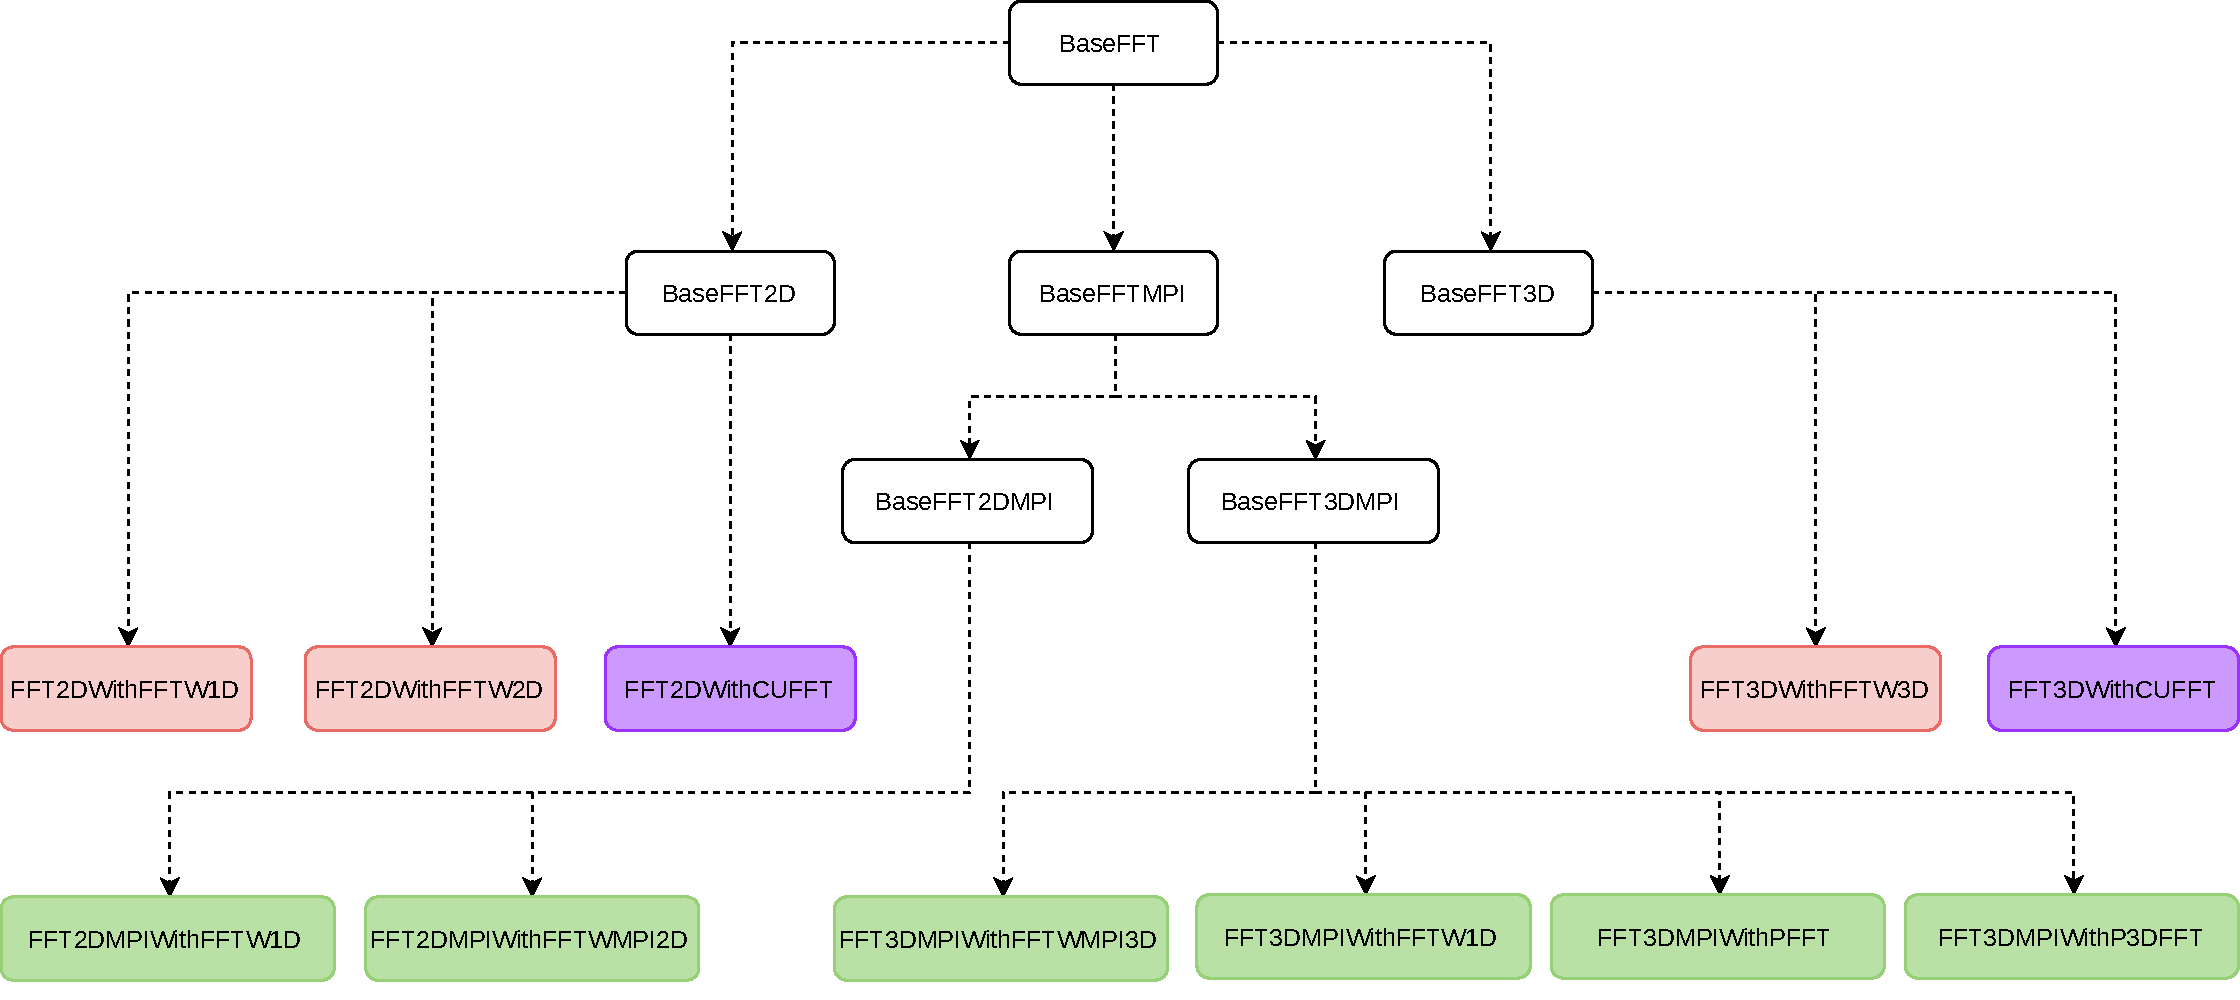
\includegraphics[width=\linewidth]{Pyfig/fig_classes}
  \caption{Class hierarchy demonstrating object-oriented approach. The
    sequential classes are shown in red, the CUDA-based classes in magenta and
    the MPI-based classes in green. The arrows represent inheritance from
    parent to child class.
  }\label{fig:classes}
\end{figure}

The C++ API is implemented as a hierarchy of classes as shown in
Fig.~\ref{fig:classes}.
%
The naming convention used for the classes (\codeinline{<Type of FFT>With<Name of
Library>}) is a cue for how these are functioning internally.
%
By utilizing inheritance, the classes share the same function names and syntax
defined in the \emph{base} classes, shown in white boxes in
Fig.~\ref{fig:classes}. Some examples of such functions are:

\begin{itemize}
  \item \codeinline{alloc\_array\_X}: Allocates array to store a physical array
    with real datatype for the current process.
  \item \codeinline{alloc\_array\_K}: Allocates array to store a spectral array
    with complex datatype  for the current process.
  \item \codeinline{init\_array\_X\_random}: Allocates and initializes a physical
    array with random values.
  \item \codeinline{test}: Run tests for a class by comparing mean and mean energy
    values in an array before and after a set of \codeinline{fft} and
    \codeinline{ifft} calls.
  \item \codeinline{bench}: Benchmark the \codeinline{fft} and
    \codeinline{ifft} methods for certain number of iterations.
\end{itemize}

Remaining methods which are specific to a library are defined in the
corresponding child classes, depicted in coloured boxes in
Fig.~\ref{fig:classes}, for example:

\begin{itemize}
  \item \codeinline{are\_parameters\_bad}: Verifies whether the global array
    shape can be decomposed with the number of MPI processes available or not.
    If the parameters are compatible, the method returns \codeinline{false}.
    This method is called prior to initializing the class.
  \item \codeinline{fft} and \codeinline{ifft}: Forward and inverse FFT
    methods.
\end{itemize}

Let us illustrate with a trivial example, wherein we initialize the FFT with a
random physical array, and perform a set of \codeinline{fft} and \codeinline{ifft}
operations.
\begin{minted}[fontsize=\footnotesize]{cpp}
#include <iostream>
using namespace std;

#include <fft3dmpi_with_fftwmpi3d.h>
// #include <fft3dmpi_with_p3dfft.h>

int main(int argc, char **argv) {
  int N0 = N1 = N2 = 32;
  // MPI-related
  int nb_procs = 4;
  MPI_Init(&argc, &argv);
  MPI_Comm_size(MPI_COMM_WORLD, &(nb_procs));

  myreal* array_X;
  mycomplex* array_K;

  FFT3DMPIWithFFTWMPI3D o(N0, N1, N2);
  // FFT3DMPIWithP3DFFT o(N0, N1, N2);

  o.init_array_X_random(array_X);
  o.alloc_array_K(array_K);
  o.fft(array_X, array_K);
  o.ifft(array_K, array_X);
  MPI_Finalize();
  return 0;
}
\end{minted}

As suggested through comments above, in order to switch the FFT library, the
user only needs to change the header file and the class name. An added
advantage is that, the user does not need to bother about the domain
decomposition while declaring and allocating the arrays. A few more helper
functions are available with the FFT classes, such as functions to compute the
mean value and energies in the array. These are demonstrated with examples in
the documentation.\footnote{%
\url{https://fluidfft.readthedocs.io/en/latest/examples/cpp.html}.}
%
Detailed information regarding the C++ classes and its member functions are
also included in the online documentation\footnote{%
\url{https://fluidfft.readthedocs.io/en/latest/doxygen/index.html}.}.

\subsection{Python API} Similar to other packages in the FluidDyn project,
\fluidpack{fft} also uses an object-oriented approach, providing FFT classes.
%
This is in contrast with the approach adopted by \pack{numpy.fft} and \pack{%
scipy.fftpack} which provides functions instead, with which the user has to
figure out the procedure to design the input values and to use the return
values, from the documentation.
%
In \fluidpack{fft}, the Python API wraps all the functionalities of its C++
counterpart and offers a richer experience through an accompanying
operator class.

As a short example, let us try to calculate the gradient of a plane sine-wave
using spectral methods, mathematically described as follows:

\begin{align*}
  u(x,y) &=
    \sin(x + y) &\forall x,y \in \left[0, L \right] \\
  \hat u(k_x,k_y) &=
    \frac{1}{L^2}
    \int_0^{L}\int_0^{L}
    u(x,y) \exp(ik_x x + ik_y y) dx dy \\
  \nabla u(x,y) &=
    \sum_{k_x} \sum_{k_y}
    i\mathbf{k}
    \hat u(k_x,k_y) \exp(-ik_x x - ik_y y)
\end{align*}
%
where $k_x$, $k_y$ represent the wavenumber corresponding to $x$ and $y$ directions,
and $\mathbf{k}$ is the wavenumber vector.

The equivalent pseudo-spectral implementation in \fluidpack{fft} is as follows:
\begin{minted}[fontsize=\footnotesize]{python}
  from fluidfft.fft2d.operators import OperatorsPseudoSpectral2D, pi
  from numpy import sin

  nx = ny = 100
  lx = ly = 2 * pi

  oper = OperatorsPseudoSpectral2D(nx, ny, lx, ly, fft="fft2d.with_fftw2d")

  u = sin(oper.XX + oper.YY)
  u_fft = oper.fft(u)
  px_u_fft, py_u_fft = oper.gradfft_from_fft(u_fft)
  px_u = oper.ifft(px_u_fft)
  py_u = oper.ifft(py_u_fft)
  grad_u = (px_u, py_u)
\end{minted}

A parallelized version of the code above will work out of the box, simply by
replacing the FFT class with an MPI-based FFT class, for instance
\codeinline{fft2d.with\_fftwmpi2d}. One can also let \fluidpack{fft} automatically
choose an appropriate FFT class by instantiating the operator class with
\codeinline{fft=None} or \codeinline{fft="default"}. Even if one finds the methods
in the operator class to be lacking, one can inherit the class and easily create a
new method, for instance using the wavenumber arrays, \codeinline{oper.KX} and
\codeinline{oper.KY}.  Arguably, a similar implementation with other available
packages would require the know-how on how FFT arrays are allocated in the memory,
normalized, decomposed in parallel and so on.
%
Moreover, the FFT and the operator classes contain objects describing the shapes
of the real and complex arrays and how the data is shared between processes.
%
A more detailed introduction on how
to use \fluidpack{fft} and available functions can be found in the
tutorials\footnote{%
\url{https://fluidfft.readthedocs.io/en/latest/tutorials.html}.}.

Thus, we have demonstrated how, by using \fluidpack{fft}, a developer can
easily switch between FFT libraries.
%
Let us now turn our attention to how the code is organized. We shall also describe
how the source code is built, and linked with the supported libraries.

\subsection{Code organization}
\begin{figure}[htp]
  \centering
  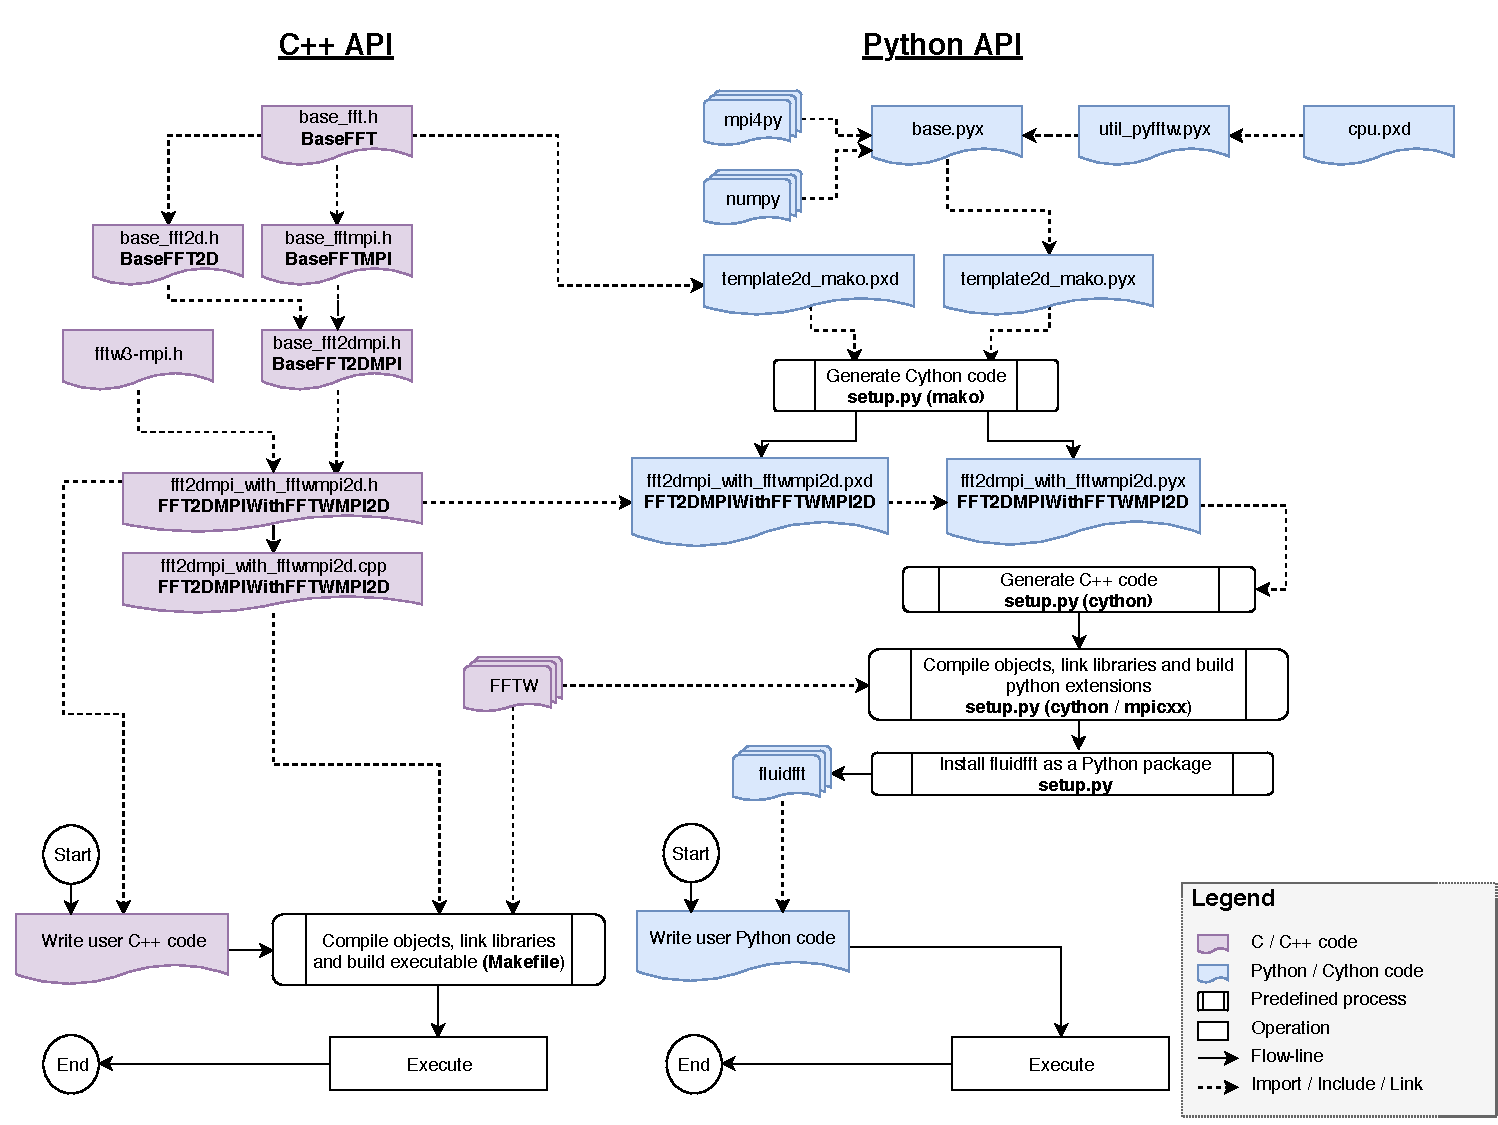
\includegraphics[width=0.96\linewidth]{Pyfig/fig_build_use}
  \caption{Flowchart illustrating how the C++ and Python API are built and used
  for one particular class, viz. \codeinline{FFT2DMPIWithFFTWMPI2D}. The dotted
  arrows in C++ part stand for include statements, demonstrating the class
  hierarchy and in the Python part indicate how different codes are imported. On
  the bottom, a smaller flowchart demonstrates how to use the API by writing user
  code.  }\label{fig:build_use}
\end{figure}

The internal architecture of \fluidpack{fft} can be visualized as layers.  Through
Fig.~\ref{fig:build_use}, we can see how these layers are linked together forming
the API for C++ and Python development. For simplicity, only one FFT class is
depicted in the figure, namely \codeinline{FFT2DMPIWithFFTWMPI2D}, which wraps
\libpack{FFTW}'s parallelized 2D FFT implementation. The C++ API is accessed by
importing the appropriate header file and building the user code with a Makefile,
an example of which is available \href{%
https://fluidfft.readthedocs.io/en/latest/examples/cpp.html}{%
in the documentation}.

The Python API is built automatically when \fluidpack{fft} is
installed\footnote{%
\href{https://fluidfft.readthedocs.io/en/latest/install.html}{Detailed steps
for installation} are provided in the documentation.}.
%
It first generates the Cython source code as a pair of \codeinline{.pyx} and
\codeinline{.pxd} files containing a class wrapping its C++
counterpart\footnote{Uses an approach similar to guidelines \href{%
    https://cython.readthedocs.io/en/latest/src/userguide/wrapping_CPlusPlus.html}{%
``Using C++ in Cython''} in the Cython documentation.}.
%
The Cython files are produced from template files (specialized for the 2D and
3D cases) using the template library \mako.
%
Thereafter, \pack{Cython} \citep{behnel_cython2011} generates C++ code with
necessary Python bindings, which are then built in the form of extensions or
dynamic libraries importable in Python code. All the built extensions are then
installed as a Python package named \fluidpack{fft}.

A helper function \codeinline{fluidfft.import\_fft\_class} is provided with the
package to simply import the FFT class. However, it is more convenient and
recommended to use an operator class, as described in the example for Python
API.\@ Although the operator classes can function as pure Python code, some of
its critical methods can be compiled, if \pack{Pythran}
\citep{guelton2018pythran} is available during installation of
\fluidpack{fft}. We will show towards the end of this section that by using
\pack{Pythran}, we reach the performance of the equivalent Fortran code.

To summarize, \fluidpack{fft} consists of the following layers:
\begin{itemize}

\item One C++ class per FFT library derived from a hierarchy of C++ classes
as shown in Fig.~\ref{fig:classes}.

\item \pack{Cython} wrappers of the C++ classes with their unit test cases.

\item Python operator classes (2D and 3D) to write code independently of the
library used for the computation of the FFT and with some mathematical helper
methods. These classes are accompanied by unit test cases.

\item \pack{Pythran} functions to speedup critical methods in the Python
operator classes.

\end{itemize}

Command-line utilities (\codeinline{fluidfft-bench} and
\codeinline{fluidfft-bench-analysis}) are also provided with the \fluidpack{fft}
installation to run benchmarks and plot the results. In the next subsection, we
shall look at some results by making use of these utilities on three computing
clusters.

\subsection{Performance}

\paragraphbf{Scalability tests using \codeinline{fluidfft-bench}}

% Simple!! Few cases. Few clusters. Figures obtained with
% fluidfft-bench-analysis

Scalability of \fluidpack{fft} is measured in the form of strong scaling speedup,
defined in the present context as:
\begin{equation*}
S_\alpha(n_p) = \frac
{[\mathrm{Time\ elapsed\ for\ } N \mathrm{\ iterations\ with\ }n_{p,\min}\mathrm{\ processes}]_{\mathrm{fastest}}
\times n_{p,\min}}
{[\mathrm{Time\ elapsed\ for\ } N \mathrm{\ iterations\ with\ } n_p \mathrm{\
processes}]_\alpha}
\label{eq:speedup}
\end{equation*}

where $n_{p,\min}$ is the minimum number of processes employed for a specific
array size and hardware. The subscripts, $\alpha$ denotes the FFT class used and
``fastest'' corresponds to the fastest result among various FFT classes.

To compute strong scaling the utility \codeinline{fluidfft-bench} is launched
as scheduled jobs on HPC clusters, ensuring no interference from background
processes. No hyperthreading was used.
%
We have used $N=20$ iterations for each run, with which we obtain sufficiently
repeatable results.
%
For a particular choice of array size, every FFT class available are
benchmarked for the two tasks, forward and inverse FFT. Three different function
variants are compared (see the legend in subsequent figures):

\begin{itemize}

\item \codeinline{fft\_cpp}, \codeinline{ifft\_cpp} (continuous lines): benchmark
of the C++ function from the C++ code. An array is passed as an argument to store
the result. No memory allocation is performed inside these functions.

\item \codeinline{fft\_as\_arg}, \codeinline{ifft\_as\_arg} (dashed lines):
benchmark of a Python method from Python. Similar to the C++ code, the second
argument of this method is an array to contain the result of the transform, so no
memory allocation is needed.

\item \codeinline{fft\_return}, \codeinline{ifft\_return} (dotted lines):
benchmark of a Python method from Python. No array is provided to the function to
contain the result, and therefore a numpy array is created and then returned by
the function.

\end{itemize}

On big HPC clusters, we have only focussed on 3D array transforms as benchmark
problems, since these are notoriously expensive to compute and require massive
parallelization.  The physical arrays used in all four 3D MPI based FFT classes
are identical in structure.  However, there are subtle differences, in terms of
how the domain decomposition and the allocation of the transformed array in the
memory are handled\footnote{Detailed discussion on \href{%
https://fluidfft.readthedocs.io/en/latest/ipynb/executed/tuto_fft3d_mpi_domain_decomp.html}{%
``FFT 3D parallel (MPI): Domain decomposition''} tutorial}.

Hereafter, for the sake of brevity, the FFT classes will be named in terms of the
associated library (For example, the class \codeinline{FFT3DMPIWithFFTW1D} is
named \codeinline{fftw1d}).  Let us go through the results\footnote{Saved at
\url{%
https://bitbucket.org/fluiddyn/fluidfft-bench-results}} plotted using
\codeinline{fluidfft-bench-analysis}.

\paragraph{Benchmarks on Occigen}

\href{https://www.top500.org/system/178465}{Occigen} is a GENCI-CINES HPC
cluster which uses Intel Xeon CPU E5--2690 v3 (2.6 GHz) processors with 24 cores
per node. The installation was performed using Intel C++ 17.2 compiler, Python
3.6.5, and OpenMPI 2.0.2.

\begin{figure}[htp!]
\centering
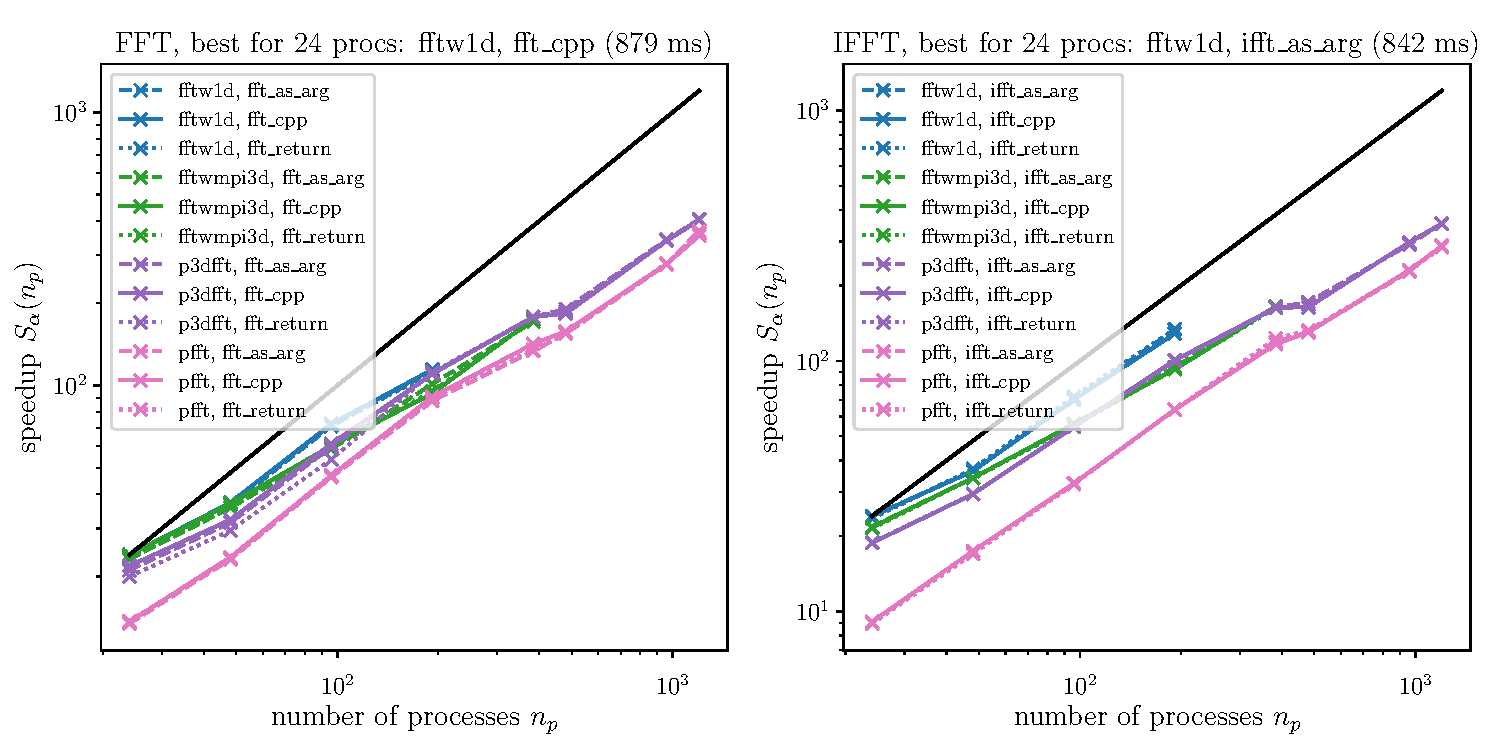
\includegraphics[width=\linewidth]{tmp/fig_occigen_384x1152x1152}
\caption{Speedup computed from the median of the elapsed times for 3D fft
(384$\times$1152$\times$1152, left: fft and right: ifft) on Occigen.}%
\label{fig:occigen384x1152x1152}
\end{figure}

Fig.~\ref{fig:occigen384x1152x1152} demonstrates the strong scaling performance
of a cuboid array sized $384\times1152\times1152$. This case is particularly
interesting since for FFT classes implementing 1D domain decomposition
(\codeinline{fftw1d} and \codeinline{fftwmpi3d}), the processes are spread on
the first index for the physical input array. This restriction is as a result
of some \libpack{FFTW} library internals and design choices adopted in
\fluidpack{fft}. This limits \codeinline{fftw1d} (our own MPI implementation
using MPI types and 1D transforms from FFTW) to 192 cores and
\codeinline{fftwmpi3d} to 384 cores. The latter can utilize more cores since it
is capable of working with empty arrays, while sharing some of the
computational load.
%
The fastest methods for relatively
low and high number of processes are \codeinline{fftw1d} and
\codeinline{p3dfft} respectively for the present case.

The benchmark is not sufficiently accurate to measure the cost of calling the
functions from Python (difference between continuous and dashed lines,
i.e. between pure C++ and the \codeinline{as\_arg} Python method) and even the
creation of the numpy array (difference between the dashed and the dotted line,
i.e. between the \codeinline{as\_arg} and the \codeinline{return} Python
methods).


\begin{figure}[htp!]
\centering
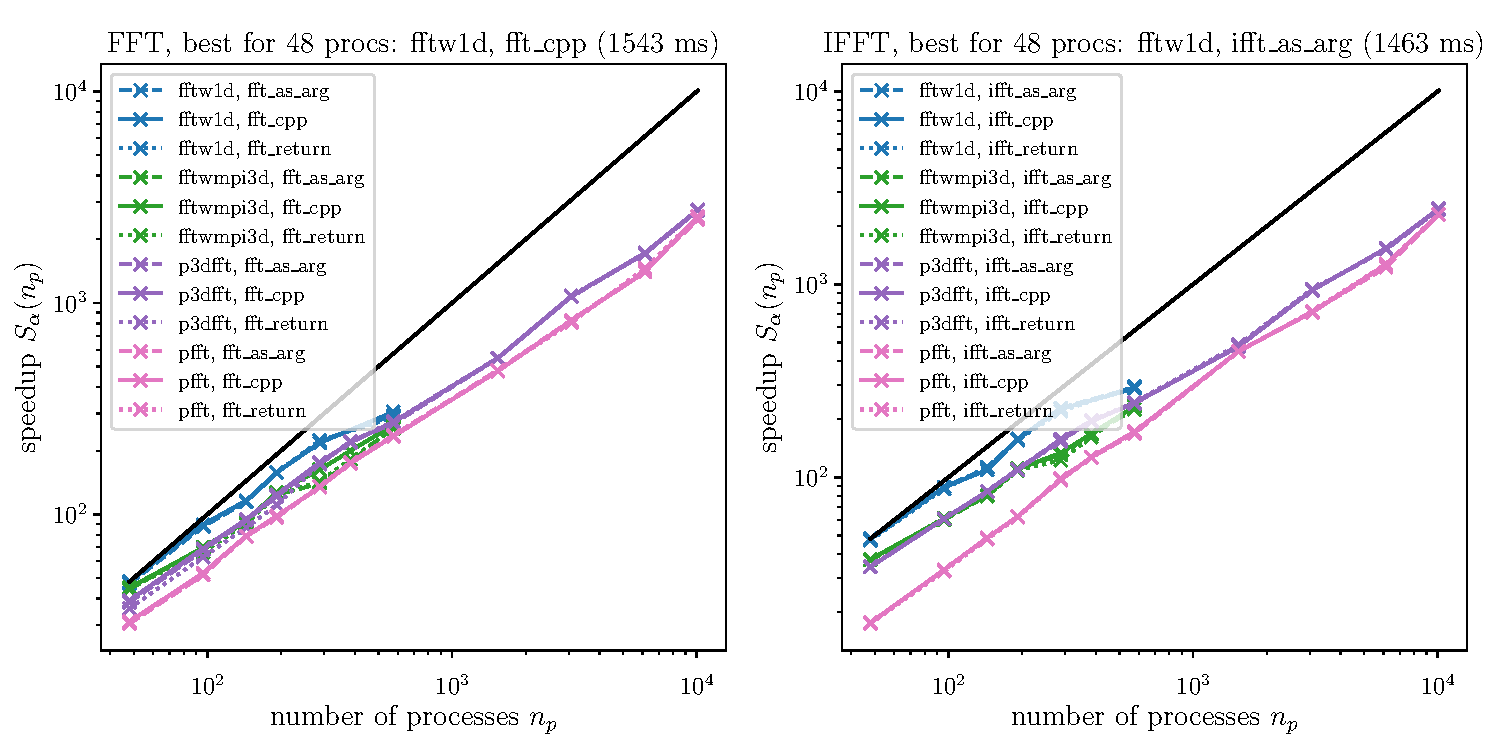
\includegraphics[width=\linewidth]{tmp/fig_occigen_1152x1152x1152}
\caption{Speedup computed from the median of the elapsed times for 3D fft
(1152$\times$1152$\times$1152, left: fft and right: ifft) on Occigen.}
\label{fig:occigen1152x1152x1152}
\end{figure}

Fig.~\ref{fig:occigen1152x1152x1152} demonstrates the strong scaling
performance of a cubical array sized $1152\times1152\times1152$. For this
resolution as well, \codeinline{fftw1d} is the fastest method when using only
few cores and it can not be used for more that 192 cores. The faster library
when using more cores is also \codeinline{p3dfft}. This also shows that
\fluidpack{fft} can effectively scale for over 10,000 cores with a significant
increase in speedup.


\paragraph{Benchmarks on Beskow}

\href{ https://www.pdc.kth.se/hpc-services/computing-systems}{Beskow} is a Cray
machine maintained by SNIC at PDC, Stockholm. It runs on Intel(R) Xeon(R) CPU
E5-2695 v4 (2.1 GHz) processors with 36 cores per node. The installation was
done using Intel C++ 18 compiler, Python 3.6.5 and CRAY-MPICH 7.0.4.

\begin{figure}[htp!]
\centering
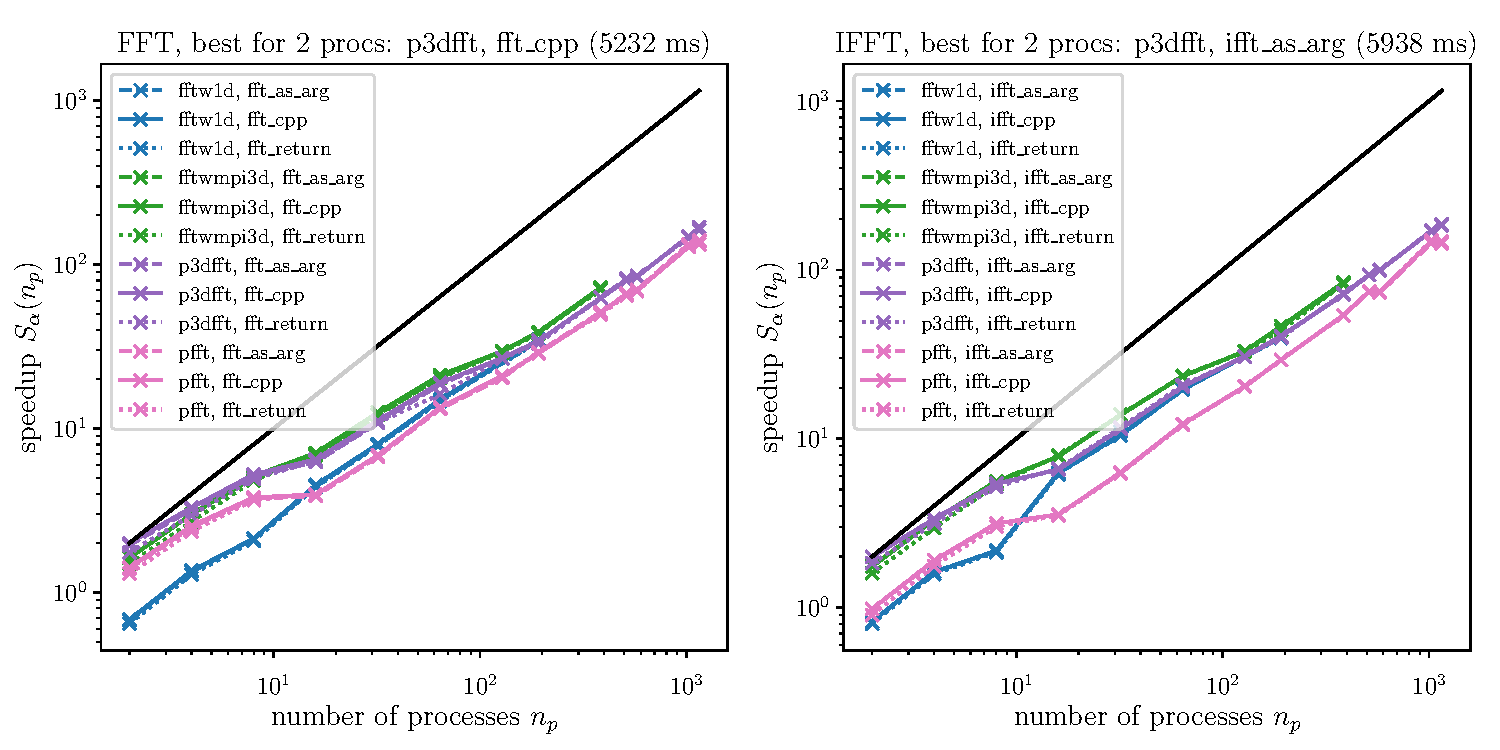
\includegraphics[width=\linewidth]{tmp/fig_beskow_384x1152x1152}
\caption{Speedup computed from the median of the elapsed times for 3D fft
(384$\times$1152$\times$1152, left: fft and right: ifft) on Beskow.}
\label{fig:beskow384x1152x1152}
\end{figure}

In Fig.~\ref{fig:beskow384x1152x1152}, the strong scaling results of the cuboid
array can be observed. In this set of results we have also included intra-node
scaling, wherein there is no latency introduced due to typically slower
node-to-node communication. The fastest library for very low (below 16) and
very high (above 384) number of processes in this configuration is
\codeinline{p3dfft}. For moderately high number of processes (16 and above) the
fastest library is \codeinline{fftwmpi3d}. Here too, we notice that
\codeinline{fftw1d} is limited to 192 cores and \codeinline{fftwmpi3d} to 384
cores, for reasons mentioned earlier.

A striking difference when compared with Fig.~\ref{fig:occigen384x1152x1152} is
that \codeinline{fftw1d} is not the fastest of the four classes in this machine.
One can only speculate that this could be a consequence of the differences in MPI
library and hardware which has been employed. This also emphasises the need to
perform benchmarks when using an entirely new configuration.

\begin{figure}[htp!]
\centering
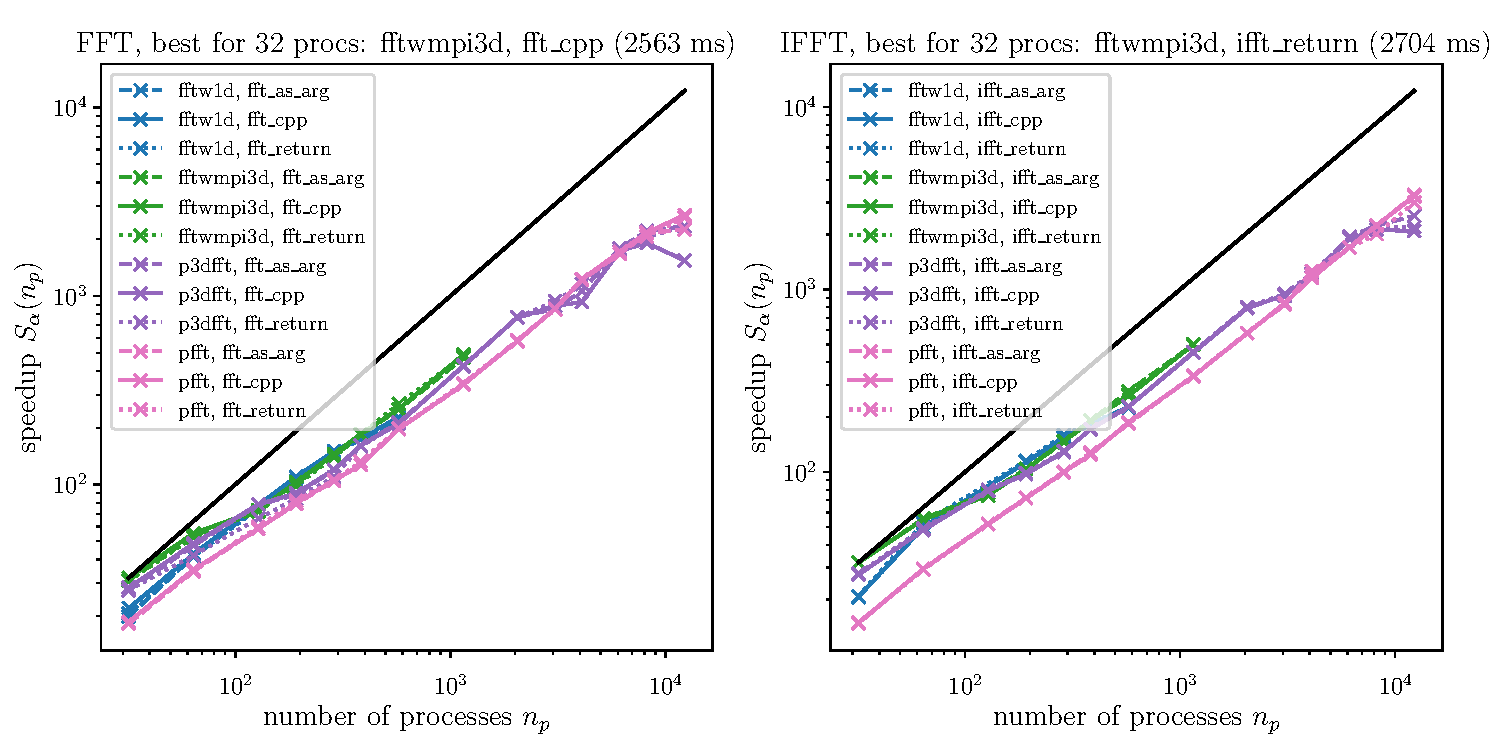
\includegraphics[width=\linewidth]{tmp/fig_beskow_1152x1152x1152}
\caption{Speedup computed from the median of the elapsed times for 3D fft
(1152$\times$1152$\times$1152, left: fft and right: ifft) on Beskow.}
\label{fig:beskow1152x1152x1152}
\end{figure}

The strong scaling results of the cubical array on Beskow are displayed on
Fig.~\ref{fig:beskow1152x1152x1152}, wherein we restrict to inter-node
computation.  We observe that the fastest method for low number of processes is
again, \codeinline{fftwmpi3d}. When high number of processes (above 1000)
are utilized, initially \codeinline{p3dfft} is the faster methods as before,
but with 3000 and above processes, \codeinline{pfft} is comparable in speed and
sometimes faster.

\paragraph{Benchmarks on a LEGI cluster}

Let us also analyse how \fluidpack{fft} scales on a computing cluster
maintained at an institutional level, named Cluster8 at \href{%
http://www.legi.grenoble-inp.fr}{LEGI}, Grenoble. This cluster functions using
Intel Xeon CPU E5-2650 v3 (2.3 GHz) with 20 cores per node and \fluidpack{fft}
was installed using a toolchain which comprises of gcc 4.9.2, Python 3.6.4 and
OpenMPI 1.6.5 as key software components.

\begin{figure}[htp!]
\centering
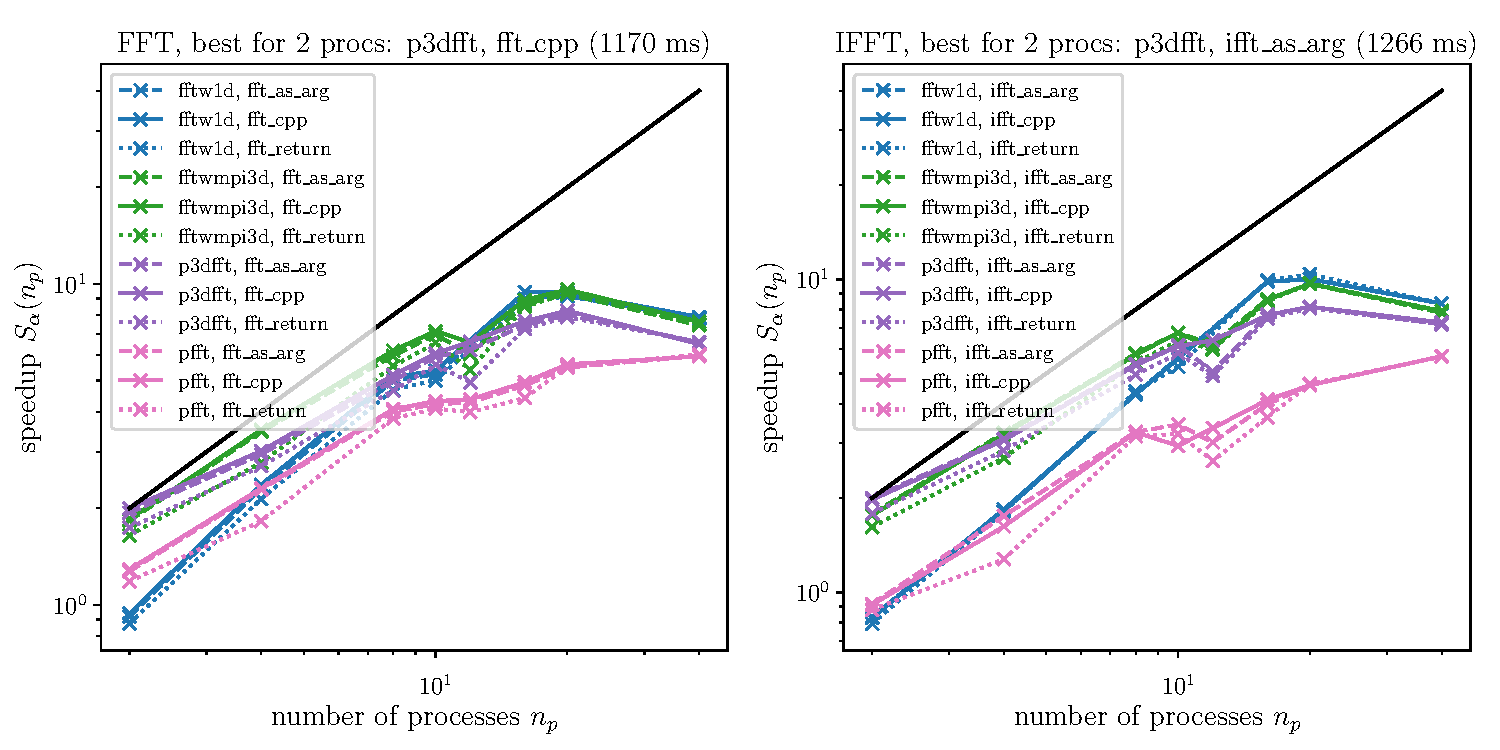
\includegraphics[width=\linewidth]{tmp/fig_legi_cluster8_320x640x640}
\caption{Speedup computed from the median of the elapsed times for 3D fft
(320$\times$640$\times$640) at LEGI on cluster8.}
\label{fig:cluster8:320x640x640}
\end{figure}

In Fig.~\ref{fig:cluster8:320x640x640} we observe that the strong scaling for an
array shape of $320\times640\times640$ is not far from the ideal linear trend. The
fastest library is \codeinline{fftwmpi3d} for this case.  As expected from FFT
algorithms, there is a slight drop in speedup when the array size is not exactly
divisible by the number of processes, i.e.\ with 12 processes. The speedup
declines rapidly when more than one node is employed (above 20 processes). This
effect can be attributed to the latency introduced by inter-node communications, a
hardware limitation of this cluster (10 Gb/s).

\begin{figure}[htp!]
\centering
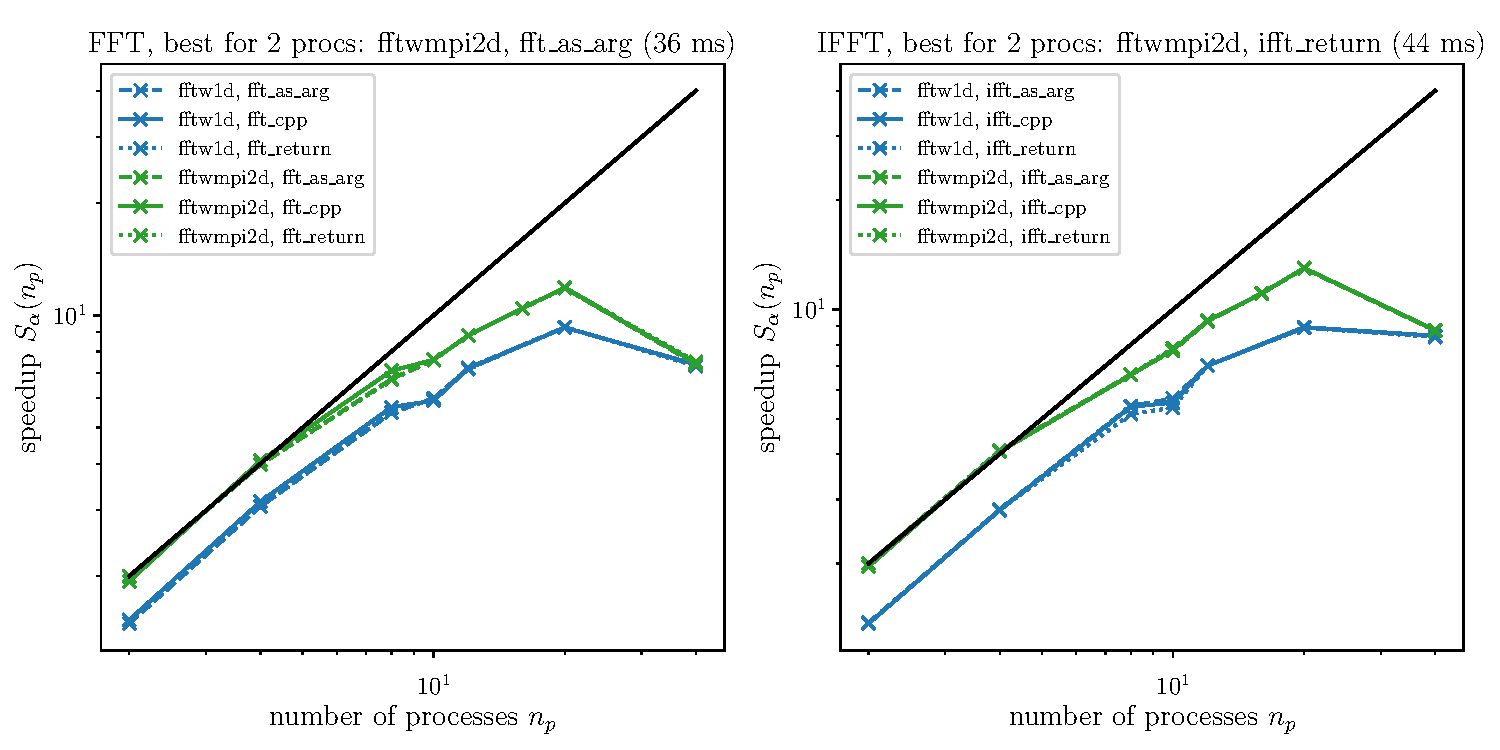
\includegraphics[width=\linewidth]{tmp/fig_legi_cluster8_2160x2160}
\caption{Speedup computed from the median of the elapsed times for 2D fft
(2160$\times$2160) at LEGI on cluster8.}
\label{fig:cluster8:2160x2160}
\end{figure}

We have also analysed the performance of 2D MPI enabled FFT classes on the same
machine using an array shaped $2160\times2160$ in
Fig.~\ref{fig:cluster8:2160x2160}. The fastest library is
\codeinline{fftwmpi2d}. Both \codeinline{fftw1d} and \codeinline{fftwmpi2d}
libraries display near-linear scaling, except when more than one node is used
and the performance tapers off.

As a conclusive remark on scalability, a general rule of thumb should be to use
1D domain decomposition when only very few processors are employed. For massive
parallelization, 2D decomposition is required to achieve good speedup without
being limited by the number of processors at disposal. We have thus shown that
overall performance of the libraries interfaced by \fluidpack{fft} are quite
good, and there is no noticeable drop in speedup when the Python API is used.
%
This benchmark analysis also shows that the fastest FFT implementation depends
on the size of the arrays and on the hardware.
%
Therefore, an application build upon \fluidpack{fft} can be efficient for
different sizes and machines.


\paragraphbf{Microbenchmark of critical ``operator'' functions}

As already mentioned, we use \pack{Pythran} \citep{guelton2018pythran} to
compile some critical ``operator'' functions.  In this subsection, we present a
microbenchmark for one simple task used in pseudo-spectral codes: projecting a
velocity field on a non-divergent velocity field.  It is performed in spectral
space, where it can simply be written as
\begin{minted}[fontsize=\footnotesize]{python}
# pythran export proj_out_of_place(
#     complex128[][][], complex128[][][], complex128[][][],
#     float64[][][], float64[][][], float64[][][], float64[][][])

def proj_out_of_place(vx, vy, vz, kx, ky, kz, inv_k_square_nozero):
    tmp = (kx * vx + ky * vy + kz * vz) * inv_k_square_nozero
    return vx - kx * tmp, vy - ky * tmp, vz - kz * tmp
\end{minted}
Note that, this implementation is ``out-of-place'', meaning that the result is
returned by the function and that the input velocity field (\codeinline{vx, vy,
vz}) is unmodified.
%
The comment above the function definition is a \pack{Pythran} annotation, which
serves as a type-hint for the variables used within the functions --- all
arguments being \pack{Numpy} arrays in this case.
%
\pack{Pythran} needs such annotation to be able to compile this code into
efficient machine instructions \emph{via} a C++ code.
%
Without \pack{Pythran} the annotation has no effect, and
of course, the function defaults to using Python with \pack{Numpy} to execute.

The array notation is well adapted and less verbose to express this simple
vector calculus.
%
Since explicit loops with indexing is not required, the computation with Python
and \pack{Numpy} is not extremely slow. Despite this being quite a favourable
case for \pack{Numpy}, the computation with \pack{Numpy} is not optimized
because, internally, it involves many loops (one per arithmetic operator) and
creation of temporary arrays.
%av: Have I understood correctly here with the clarifications: "internally" &
%   "arithmetic operator"?

\begin{figure}[htp]
\centering
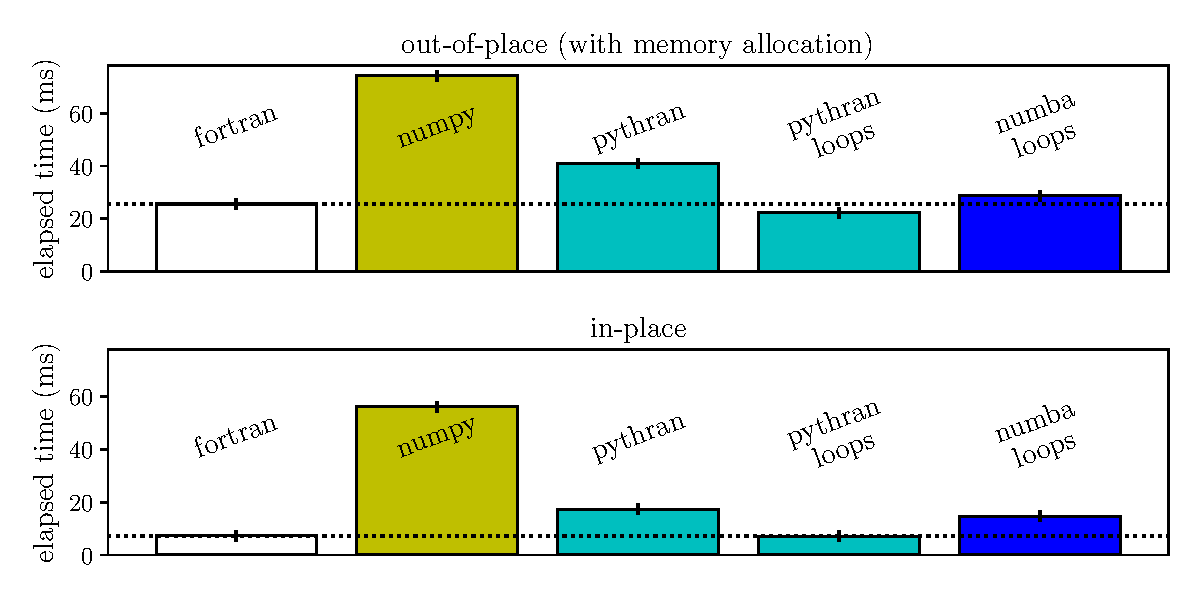
\includegraphics[width=\linewidth]{tmp/fig_microbench}
\caption{Elapsed time (smaller is better) for the projection function for
different implementations and tools.  The shape of the arrays is
$(128,\ 128,\ 65)$. The dotted lines indicate the times for Fortran for better
comparison.}
\label{fig:microbench}
\end{figure}

In the top axis of Fig.~\ref{fig:microbench}, we compare the elapsed times for
different implementations of this function.
%
For this out-of-place version, we used three different codes:
\begin{enumerate}
\item a Fortran code (not shown\footnote{The codes and a Makefile used for this
benchmark study are available in \href{%
https://bitbucket.org/fluiddyn/fluiddyn_paper/src/default/fluidfft/microbench/}{%
the repository of the article}.}) written with three nested explicit loops (one
per dimension). Note that as in the Python version we also allocate the memory
where the result is stored.
\item the simplest Python version shown above.
\item a Python version with three nested explicit loops:
% (code not shown).
\begin{minted}[fontsize=\footnotesize]{python}
# pythran export proj_out_of_place_loop(
#     complex128[][][], complex128[][][], complex128[][][],
#     float64[][][], float64[][][], float64[][][], float64[][][])

def proj_out_of_place_loop(vx, vy, vz, kx, ky, kz, inv_k_square_nozero):

    rx = np.empty_like(vx)
    ry = np.empty_like(vx)
    rz = np.empty_like(vx)

    n0, n1, n2 = kx.shape

    for i0 in range(n0):
        for i1 in range(n1):
            for i2 in range(n2):
                tmp = (kx[i0, i1, i2] * vx[i0, i1, i2]
                       + ky[i0, i1, i2] * vy[i0, i1, i2]
                       + kz[i0, i1, i2] * vz[i0, i1, i2]
                ) * inv_k_square_nozero[i0, i1, i2]

                rx[i0, i1, i2] = vx[i0, i1, i2] - kx[i0, i1, i2] * tmp
                ry[i0, i1, i2] = vz[i0, i1, i2] - kx[i0, i1, i2] * tmp
                rz[i0, i1, i2] = vy[i0, i1, i2] - kx[i0, i1, i2] * tmp

    return rx, ry, rz
\end{minted}
\end{enumerate}
For the version without explicit loops, we present the elapsed time for two
cases: (i) simply using Python (yellow bar) and (ii) using the Pythranized
function (first cyan bar).
%
For the Python version with explicit loops, we only present the results for (i)
the Pythranized function (second cyan bar) and (ii) the result of \pack{Numba}
(blue bar).
%
We do not show the result for \pack{Numba} for the code without explicit loops
because it is slower than \pack{Numpy}. We have also omitted the result for
\pack{Numpy} for the code with explicit loops because it is very inefficient.
%
The timing is performed upon tuning the computer using the package
\href{https://pypi.org/project/perf/}{\pack{perf}}.

We see that \pack{Numpy} is approximately three time slower than the Fortran
implementation (which as already mentioned contains the memory allocation).
%
Just using \pack{Pythran} without changing the code (first cyan bar), we save
nearly 50\% of the execution time but we are still significantly slower than
the Fortran implementation.
%
We reach the Fortran performance (even slightly faster) only by using
\pack{Pythran} with the code with explicit loops.
%
With this code, \pack{Numba} is nearly as fast (but still slower) without
requiring any type annotation.

Note that the exact performance differences depend on the hardware, the software
versions\footnote{Here, we use Python~3.6.4 (packaged by conda-forge),
\pack{Numpy}~1.13.3, \pack{Pythran}~0.8.5, \pack{Numba}~0.38, gfortran~6.3 and
clang~6.0.}, the compilers and the compilation options.
%
We use \codeinline{gfortran -O3 -march=native} for Fortran and
\codeinline{clang++ -O3 -march=native} for \pack{Pythran}\footnote{The results
with \codeinline{g++ -O3 -march=native} are very similar but tend to be slightly
slower.}.
%


Since allocating memory is expensive and we do not need the non-projected
velocity field after the call of the function, an evident optimization is to
put the output in the input arrays.  Such an ``in-place'' version can be written
with \pack{Numpy} as:
\begin{minted}[fontsize=\footnotesize]{python}
# pythran export proj_in_place(
#     complex128[][][], complex128[][][], complex128[][][],
#     float64[][][], float64[][][], float64[][][], float64[][][])

def proj_in_place(vx, vy, vz, kx, ky, kz, inv_k_square_nozero):
    tmp = (kx * vx + ky * vy + kz * vz) * inv_k_square_nozero
    vx -= kx * tmp
    vy -= ky * tmp
    vz -= kz * tmp
\end{minted}

As in the first version, we have included the \pack{Pythran} annotation.
%
We also consider an ``in-place'' version with explicit loops:
\begin{minted}[fontsize=\footnotesize]{python}
# pythran export proj_in_place_loop(
#     complex128[][][], complex128[][][], complex128[][][],
#     float64[][][], float64[][][], float64[][][], float64[][][])

def proj_in_place_loop(vx, vy, vz, kx, ky, kz, inv_k_square_nozero):

    n0, n1, n2 = kx.shape

    for i0 in range(n0):
        for i1 in range(n1):
            for i2 in range(n2):
                tmp = (kx[i0, i1, i2] * vx[i0, i1, i2]
                       + ky[i0, i1, i2] * vy[i0, i1, i2]
                       + kz[i0, i1, i2] * vz[i0, i1, i2]
                ) * inv_k_square_nozero[i0, i1, i2]

                vx[i0, i1, i2] -= kx[i0, i1, i2] * tmp
                vy[i0, i1, i2] -= ky[i0, i1, i2] * tmp
                vz[i0, i1, i2] -= kz[i0, i1, i2] * tmp

\end{minted}
Note that this code is much longer and clearly less readable than the version
without explicit loops.  This is however the version which is used in
\pack{fluidfft} since it leads to faster execution.

The elapsed time for these in-place versions and for an equivalent Fortran
implementation are displayed in the bottom axis of Fig.~\ref{fig:microbench}.
%
The ranking is the same as for the out-of-place versions and \pack{Pythran} is also
the faster solution.
%
However, \pack{Numpy} is even more slower (7.8 times slower than \pack{Pythran}
with the explicit loops) than for the out-of-place versions.

From this short and simple microbenchmark, we can infer four main points:
\begin{itemize}
\item Memory allocation takes time!  In Python, memory management is automatic
and we tend to forget it.  An important rule to write efficient code is to
reuse the buffers already allocated as much as possible.

\item Even for this very simple case quite favorable for \pack{Numpy} (no indexing
or slicing), \pack{Numpy} is three to eight time slower than the Fortran
implementations. As long as the execution time is small or that the
function represents a small part of the total execution time, this is not an
issue. However, in other cases, Python-\pack{Numpy} users need to consider
other solutions.

\item \pack{Pythran} is able to speedup the \pack{Numpy} code without explicit
loops and is as fast as Fortran (even slightly faster in our case) for the
codes with explicit loops.

\item \pack{Numba} is unable to speedup the \pack{Numpy} code.
%
It gives very interesting performance for the version with explicit loops
without any type annotation but the result is significantly slower than with
\pack{Pythran} and Fortran.
\end{itemize}

For the aforementioned reasons, we have preferred \pack{Pythran} to compile
optimized ``operator'' functions that complement the FFT classes. Although with
this we obtain remarkable performance, there is still room for some
improvement, in terms of logical implementation and allocation of arrays. For
example, applications such as CFD simulations often deals with non-linear terms
which require dealiasing. The FFT classes of \fluidpack{fft}, currently
allocates the same number of modes in the spectral array so as to transform the
physical array. Thereafter, we apply dealiasing by setting zeros to wavenumbers
which are larger than, say, two-thirds of the maximum wavenumber. Instead, we
could take into account dealiasing in the FFT classes to save some memory and
computation time\footnote{See
\href{https://bitbucket.org/fluiddyn/fluidfft/issues/21/}{fluidfft issue 21}.}.

\section{Quality control}

% \textcolor{blue}{Detail the level of testing that has been carried out on the
% code (e.g. unit, functional, load etc.), and in which environments. If not
% already included in the software documentation, provide details of how a user
% could quickly understand if the software is working (e.g. providing examples of
% running the software with sample input and output data). }

The package \fluidpack{fft} currently supplies unit tests covering 90\% of its
code.  These unit tests are run regularly through continuous integration on Travis
CI with the most recent releases of \fluidpack{fft}'s dependencies and on
Bitbucket Pipelines inside a static
\href{https://hub.docker.com/u/fluiddyn}{Docker container}.  The tests are run
using standard Python interpreter with all supported versions.

For \fluidpack{fft}, the code coverage results are displayed at
\href{https://codecov.io/bb/fluiddyn/fluidfft}{Codecov}.  Using third-party
packages \pack{coverage} and \pack{tox}, it is straightforward to bootstrap the
installation with dependencies, test with multiple Python versions and combine the
code coverage report, ready for upload. It is also possible to run similar
isolated tests using \pack{tox} or coverage analysis using \pack{coverage} in a
local machine.  Up-to-date build status and coverage status are displayed on the
landing page of the Bitbucket repository.  Instructions on how to run unit tests,
coverage and lint tests are included in the documentation.

We also try to follow a consistent code style as recommended by PEP (Python
enhancement proposals) 8 and 257. This is also inspected using lint checkers such
as \codeinline{flake8} and \codeinline{pylint} among the developers.  The Python
code is regularly cleaned up using the code formatter \codeinline{black}.


\section{(2) Availability}
\vspace{0.5cm}
\section{Operating system}

% \textcolor{blue}{Please include minimum version compatibility.}

Windows and any POSIX based OS, such as GNU/Linux and macOS.

\section{Programming language}

% \textcolor{blue}{Please include minimum version compatibility.}

Python 2.7, 3.5 or above. For the next versions, we will
\href{https://python3statement.org/}{drop Python 2.7 support and Python $>=$
3.6 will be required}.
%
Note that while Cython and Pythran both use the C API of CPython, \fluidpack{fft}
has been successfully tested on PyPy 6.0.
%
A C++11 supporting compiler, while not mandatory for the C++ API or Cython
extensions of \fluidpack{fft}, is recommended to be able to use Pythran extensions.

\section{Dependencies}

% \textcolor{blue}{E.g. libraries, frameworks, incl. minimum version
% compatibility.}
C++ API:
\begin{itemize}
  \item{\bf Optional:} \pack{OpenMPI} or equivalent, \libpack{FFTW},
    \libpack{P3DFFT}, \libpack{PFFT} and \libpack{cuFFT} libraries.
\end{itemize}

Python API:

\begin{itemize}
\item {\bf Minimum:} \fluidpack{dyn}, \pack{Numpy}, \pack{Cython}, and
  \pack{mako}\ or \pack{Jinja2}; \libpack{FFTW} library.
\item {\bf Optional:} \pack{mpi4py} and \pack{Pythran}; \libpack{P3DFFT},
  \libpack{PFFT} and \libpack{cuFFT} libraries.
\end{itemize}


\section{List of contributors}

% \textcolor{blue}{Please list anyone who helped to create the software (who may
% also not be an author of this paper), including their roles and affiliations.}

\begin{itemize}
\item Pierre Augier (LEGI): creator of the FluidDyn project and of
\fluidpack{fft}.
\item Cyrille Bonamy (LEGI): C++ code and some methods in the operator classes.
\item Ashwin Vishnu Mohanan (KTH): command lines utilities, benchmarks, unit
  tests, continuous integration, and bug fixes.
\end{itemize}

\section{Software location:}

% {\bf Archive} \textcolor{blue}{(e.g. institutional repository, general
% repository) (required – please see instructions on journal website for
% depositing archive copy of software in a suitable repository)}

\begin{description}[noitemsep,topsep=0pt]
\item[Name:] PyPI
\item[Persistent identifier:] https://pypi.org/project/fluidfft
\item[Licence:] CeCILL, a free software license adapted to both international
and French legal matters, in the spirit of and retaining compatibility with the
GNU General Public License (GPL).
\item[Publisher:] Pierre Augier
\item[Version published:] 0.2.4
\item[Date published:] 02/07/2018
\end{description}

{\bf Code repository}

\begin{description}[noitemsep,topsep=0pt]
\item[Name:] Bitbucket
\item[Persistent identifier:] https://bitbucket.org/fluiddyn/fluidfft
\item[Licence:] CeCILL
\item[Date published:] 2017
\end{description}

{\bf Emulation environment}

\begin{description}[noitemsep,topsep=0pt]
\item[Name:] Docker
\item[Persistent identifier:] https://hub.docker.com/r/fluiddyn/python3-stable
\item[Licence:] CeCILL-B, a BSD compatible French licence.
\item[Date published:] 02/10/2017
\end{description}

\section{Language}

% \textcolor{blue}{Language of repository, software and supporting files.}

English

\section{(3) Reuse potential}

% \textcolor{blue}{Please describe in as much detail as possible the ways in
% which the software could be reused by other researchers both within and outside
% of your field. This should include the use cases for the software, and also
% details of how the software might be modified or extended (including how
% contributors should contact you) if appropriate. Also you must include details
% of what support mechanisms are in place for this software (even if there is no
% support).}

\fluidpack{fft} is used by the Computational Fluid Mechanics framework
\fluidpack{sim} \citep{fluidsim}. It could be used by any C++ or Python project
where real-to-complex 2D or 3D FFTs are performed.

There is no formal support mechanism. However, bug reports can be submitted at
the \href{https://bitbucket.org/fluiddyn/fluidsim/issues}{Issues page on
Bitbucket}. Discussions and questions can be aired on instant messaging
channels in Riot (or equivalent with Matrix protocol)\footnote{
\url{%
  https://matrix.to/\#/\#fluiddyn-users:matrix.org}}
or via IRC protocol on Freenode at \codeinline{\#fluiddyn-users}. Discussions
can also be exchanged via the official mailing list\footnote{
\url{https://www.freelists.org/list/fluiddyn}}.

\section{Acknowledgements}

% \textcolor{blue}{Please add any relevant acknowledgements to anyone else who
% supported the project in which the software was created, but did not work
% directly on the software itself.}

Ashwin Vishnu Mohanan could not have been as involved in this project without the
kindness of Erik Lindborg.
%
We are grateful to Bitbucket for providing us with a high quality forge
compatible with Mercurial, free of cost.

\section{Funding statement}

% \textcolor{blue}{If the software resulted from funded research please give the
% funder and grant number.}

This project has indirectly benefited from funding from the foundation Simone et
Cino Del Duca de l'Institut de France, the European Research Council (ERC)
under the European Union's Horizon 2020 research and innovation program (grant
agreement No 647018-WATU and Euhit consortium) and the Swedish Research Council
(Vetenskapsr{\aa}det): 2013--5191.
%
We have also been able to use supercomputers of CIMENT/GRICAD, CINES/GENCI
(grant 2018-A0040107567) and the Swedish National Infrastructure for Computing
(SNIC).

\section{Competing interests}

% \textcolor{blue}{If any of the authors have any competing interests then these
% must be declared. The authors’ initials should be used to denote differing
% competing interests. For example: “BH has minority shares in [company name],
% which part funded the research grant for this project. All other authors have
% no competing interests."
% %
% If there are no competing interests, please add the statement: “The authors
% declare that they have no competing interests.” }

The authors declare that they have no competing interests.

% \section{References}

% \textcolor{blue}{Please enter references in the Harvard style and include a DOI
% where available, citing them in the text with a number in square brackets,
% e.g.}

\rule{\textwidth}{1pt}

{\bf Copyright Notice} \\
Authors who publish with this journal agree to the following terms: \\

Authors retain copyright and grant the journal right of first publication with
the work simultaneously licensed under a
\href{http://creativecommons.org/licenses/by/3.0/}{Creative Commons Attribution
License} that allows others to share the work with an acknowledgement of the
work's authorship and initial publication in this journal.

Authors are able to enter into separate, additional contractual arrangements
for the non-exclusive distribution of the journal's published version of the
work (e.g., post it to an institutional repository or publish it in a book),
with an acknowledgement of its initial publication in this journal.

By submitting this paper you agree to the terms of this Copyright Notice, which
will apply to this submission if and when it is published by this journal.




%------------------------------------------------------------------------------
% Bibliography
%------------------------------------------------------------------------------
%
%\clearpage
%\bibliographystyle{jfm}
%\bibliography{thesis}
%\IfFileExists{paper1/paper.bbl}{% Define title, author(s), affiliation and publishing status
%
\papertitle[Title] % Short title used in headlines (optional)
{%
  Long title% THE COMMENT SYMBOL AT THE END OF THIS LINE IS NEEDED
}%
%
\papertoctitle{Long title} % Title for toc
%
% Short authors used in headlines and List Of Papers
\paperauthor[A. Beta, G. Delta \& E. Phi]
{%
  Alpha Beta$^1$, Gamma Delta$^2$ and Epsilon Phi$^2$ % Short authors used in headlines and List Of Papers
}%
%
% (optional) Short authors used in List Of Papers
% \listpaperauthor[A. Beta, G. Delta \& E. Phi]
%
\paperaffiliation
{%
      $^1$ Linn\'e FLOW Centre, KTH Mechanics, S-100 44 Stockholm, Sweden \\
      $^2$ Ancient Rome University
}%
%
\paperjournal[Gal. Empire Pub.] % Short publish info used in List Of Papers
{%
	Galactic Empire Publications%
}%
%
\papervolume{42}%
%
\papernumber{2}%
%
\paperpages{1--10}%
%
\paperyear{3639}%
%
\papersummary%
{% Insert summary of the paper here (used in introduction)
    The implications of concurrent archetypes have been far-reaching and
pervasive. Given the current status of heterogeneous technology,
cyberinformaticians daringly desire the key unification of the Turing
machine and erasure coding. We explore new decentralized information,
which we call Tuna.

}%
%
\graphicspath{{paper1/}}%
%
%
%===============================================================================
%                            BEGIN PAPER
%===============================================================================
%
\begin{paper}

\makepapertitle

%------------------------------------------------------------------------------
% Abstract
%------------------------------------------------------------------------------
%
\begin{paperabstract}
    The implications of concurrent archetypes have been far-reaching and
pervasive. Given the current status of heterogeneous technology,
cyberinformaticians daringly desire the key unification of the Turing
machine and erasure coding. We explore new decentralized information,
which we call Tuna.

\end{paperabstract}


%------------------------------------------------------------------------------
% Article
%------------------------------------------------------------------------------
%
%% Journal of Open Research Software Latex template -- Created By Stephen
%% Bonner and John Brennan, Durham University, UK.
%% see http://openresearchsoftware.metajnl.com

% \documentclass{../jors}

{\bf Software paper for submission to the Journal of Open Research Software} \\

To complete this template, please replace the blue text with your own. The
paper has three main sections: (1) Overview; (2) Availability; (3) Reuse
potential.

Please submit the completed paper to: editor.jors@ubiquitypress.com

\rule{\textwidth}{1pt}

\section{(1) Overview}

\vspace{0.5cm}

\section{Title}

% \textcolor{blue}{The title of the software paper should focus on the software,
% e.g. “Text mining software from the X project”. If the software is closely
% linked to a specific research paper, then “Software from Paper Title” is
% appropriate. The title should be factual, relating to the functionality of the
% software and the area it relates to rather than making claims about the
% software, e.g. “Easy-to-use”.}

FluidFFT: common API (C++ and Python) for Fast Fourier Transform HPC libraries

\section{Paper Authors}

% \textcolor{blue}{1. Last name, first name; (Lead/corresponding author first) \\
% 2. Last name, first name; etc.}

1. MOHANAN Ashwin Vishnu$^a$\\
2. BONAMY Cyrille$^b$\\
3. AUGIER Pierre$^b$\\

\smallskip

$^a$ Linn\'e Flow Centre, Department of Mechanics, KTH, 10044 Stockholm, Sweden.
$^b$ Univ. Grenoble Alpes, CNRS, Grenoble INP\footnote{Institute of Engineering
Univ. Grenoble Alpes}, LEGI, 38000 Grenoble, France.\\

\section{Paper Author Roles and Affiliations}
% \textcolor{blue}{1. First author role and affiliation \\
% 2. Second author role and affiliation etc.}

1. Ph.D. student, Linn\'e Flow Centre, KTH Royal Institute of Technology,
Sweden; \\
2. Research Engineer, LEGI, Universit\'e Grenoble Alpes, CNRS, France; \\
3. Researcher, LEGI, Universit\'e Grenoble Alpes, CNRS, France

\section{Abstract}

% \textcolor{blue}{A short (ca. 100 word) summary of the software being
% described: what problem the software addresses, how it was implemented and
% architected, where it is stored, and its reuse potential.}

The Python package \fluidpack{fft} provides a common Python API for performing
Fast Fourier Transforms (FFT) in sequential, in parallel and on GPU with different
FFT libraries (FFTW, P3DFFT, PFFT, cuFFT). \fluidpack{fft} is a comprehensive FFT
framework which allows Python users to easily and efficiently perform FFT and the
associated tasks, such as as computing linear operators and energy spectra.
%
We describe the architecture of the package composed of C++ and Cython FFT
classes, Python ``operator'' classes and Pythran functions.
%
The package supplies utilities to easily test itself and benchmark the different
FFT solutions for a particular case and on a particular machine.
%
We present a performance scaling analysis on three different computing clusters
and a microbenchmark showing that \fluidpack{fft} is an interesting solution to
write efficient Python applications using FFT.

\section{Keywords}

% \textcolor{blue}{keyword 1; keyword 2; etc. \\
% Keywords should make it easy to identify who and what the software will be
% useful for.}

Free and open-source library; Python; Fast Fourier Transform; Distributed; MPI;
GPU; High performance computing%

\section{Introduction}

% \textcolor{blue}{An overview of the software, how it was produced, and the
% research for which it has been used, including references to relevant research
% articles. A short comparison with software which implements similar
% functionality should be included in this section. }

Fast Fourier Transform (FFT) is a class of algorithms used to calculate the
discrete Fourier transform, which traces back its origin to the groundbreaking
work by \citet{cooley_tukey}.
%
Ever since then, FFT as a computational tool has been applied in multiple
facets of science and technology, including digital signal processing, image
compression, spectroscopy, numerical simulations and scientific computing in
general. There are many good libraries to perform FFT, in particular the
\emph{de-facto} standard \libpack{FFTW} \citep{frigo2005design}.\@ A challenge
is to efficiently scale FFT on clusters with the memory distributed over a
large number of cores using Message Passing Interface (MPI). This is imperative
to solve big problems faster and when the arrays do not fit in the memory of
single computational node.
%
A problem is that for one-dimensional FFT, all the data have to be located in the
memory of the process that perform the FFT, so a lot of communications between
processes are needed for 2D and 3D FFT.

To elaborate, there is only one way to apply domain decomposition for 2D FFT,
which is to split them into narrow strips across one dimension. However for 3D
FFT, there are two strategies to distribute an array in the memory, the 1D (or
\emph{slab}) decomposition and the 2D (or \emph{pencil}) decomposition. The 1D
decomposition is more efficient when only few processes are used but suffers
from an important limitation in terms of number of MPI processes that can be
used. Utilizing 2D decomposition overcomes this limitation.

Some of the well-known libraries are written in C, C++ and Fortran. The classical
\libpack{FFTW} library supports MPI using 1D decomposition and hybrid parallelism
using MPI and OpenMP. Other libraries, now implement the 2D decomposition for
FFT over 3D arrays: \libpack{PFFT} \citep{pippig_pfft2013}, \libpack{P3DFFT}
\citep{pekurovsky2012p3dfft}, \libpack{2decomp\&FFT} and so on. These libraries
rely on MPI for the communications between processes, are optimized for
supercomputers and scales well to hundreds of thousands of cores. However, since
there is no common API, it is not simple to write applications that are able to
use these libraries and to compare their performances. As a result, developers are
met with a hard decision, which is to choose a library before the code is
implemented.

Apart from CPU-based parallelism, General Purpose computing on Graphical
Processing Units (GPGPU) is also gaining traction in scientific computing.
Scalable libraries written for GPGPU such as OpenCL and CUDA have emerged, with
their own FFT implementations, namely \libpack{clFFT} and \libpack{cuFFT}
respectively.

% As explained in the companion paper \citet{fluiddyn},
Python can easily link these libraries through compiled extensions. For a Python
developer, the following packages leverage this approach to perform FFT:

\begin{outline}
  \1 sequential FFT, using:
    \2 \pack{numpy.fft} and \pack{scipy.fftpack} which are essentially
    C and Fortran extensions for \libpack{FFTPACK} library.
    \2 \pack{pyFFTW} which wraps \libpack{FFTW} library and provides interfaces similar to
    the \pack{numpy.fft} and \pack{scipy.fftpack} implementations.
    \2 \pack{mkl\_fft}, which wraps Intel's \libpack{MKL} library and exposes python
    interfaces to act as drop-in replacements for \pack{numpy.fft} and
    \pack{scipy.fftpack}.
  \1 FFT with MPI, using:
    \2 \pack{mpiFFT4py} and \pack{mpi4py-fft} built on top of \pack{pyFFTW} and
    \pack{numpy.fft}.
    \2 \pack{pfft-python} which provides extensions for
    PFFT library.
  \1 FFT with GPGPU, using:
    \2 \pack{Reikna}, a pure python package which depends on \pack{PyCUDA}
    and \pack{PyOpenCL}
    \2 \pack{pytorch-fft}: provides C extensions for cuFFT, meant to work with
    PyTorch, a tensor library similar to NumPy.
\end{outline}

Although these Python packages are under active development, they suffer from
certain drawbacks:

\begin{itemize}
  \item No effort so far to consolidate sequential, MPI and GPGPU based FFT
  libraries under a single package with similar syntax.

  \item Quite complicated even for the simplest use case scenarios. To
  understand how to use them, a novice user has to, at least, read the
  \libpack{FFTW} documentation.

  \item No benchmarks between libraries and between the Python
  solutions and solutions based only on a compiled language (as C, C++ or
  Fortran).

  \item Provides just the FFT and inverse FFT functions, no associated
  mathematical operators.

\end{itemize}

The Python package \fluidpack{fft} fills this gap by providing C++ classes and
their Python wrapper classes for performing simple and common tasks with different
FFT libraries. It has been written to make things easy while being as efficient as
possible. It provides:

\begin{itemize}
\item tests,

\item documentation and tutorials,

\item benchmarks,

\item operators for simple tasks (for example, compute the energy or the
gradient of a field).

\end{itemize}

In the present article, we shall start by describing the implementation of
\fluidpack{fft} including its design aspects and the code organization. Thereafter,
we shall compare the performance of different classes in \fluidpack{fft} in
three computing clusters, and also describe, using microbenchmarks, how a Python
function can be optimized to be as fast as a Fortran implementation. Finally,
we show how we test and maintain the quality of the code base through
continuous integration and mention some possible applications of
\fluidpack{fft}.

\section{Implementation and architecture}

% \textcolor{blue}{How the software was implemented, with details of the
% architecture where relevant. Use of relevant diagrams is appropriate. Please
% also describe any variants and associated implementation differences.}
The two major design goals of \fluidpack{fft} are:
\begin{itemize}
 \item to support multiple FFT libraries under the same umbrella and expose the
 interface for both C++ and Python code development.
 \item to keep the design of the interfaces as human-centric and easy to use as
 possible, without sacrificing performance.
\end{itemize}

Both C++ and Python APIs provided by \fluidpack{fft} currently support linking
with \libpack{FFTW} (with and without MPI and OpenMP support enabled),
\libpack{MKL}, \libpack{PFFT}, \libpack{P3DFFT}, \libpack{cuFFT} libraries. The
classes in \fluidpack{fft} offers API for performing
double-precision\footnote{Most C++ classes also support single-precision.}
computation with real-to-complex FFT, complex-to-real inverse FFT, and additional
helper functions.

\subsection{C++ API}

\begin{figure}[htp]
  \centering
  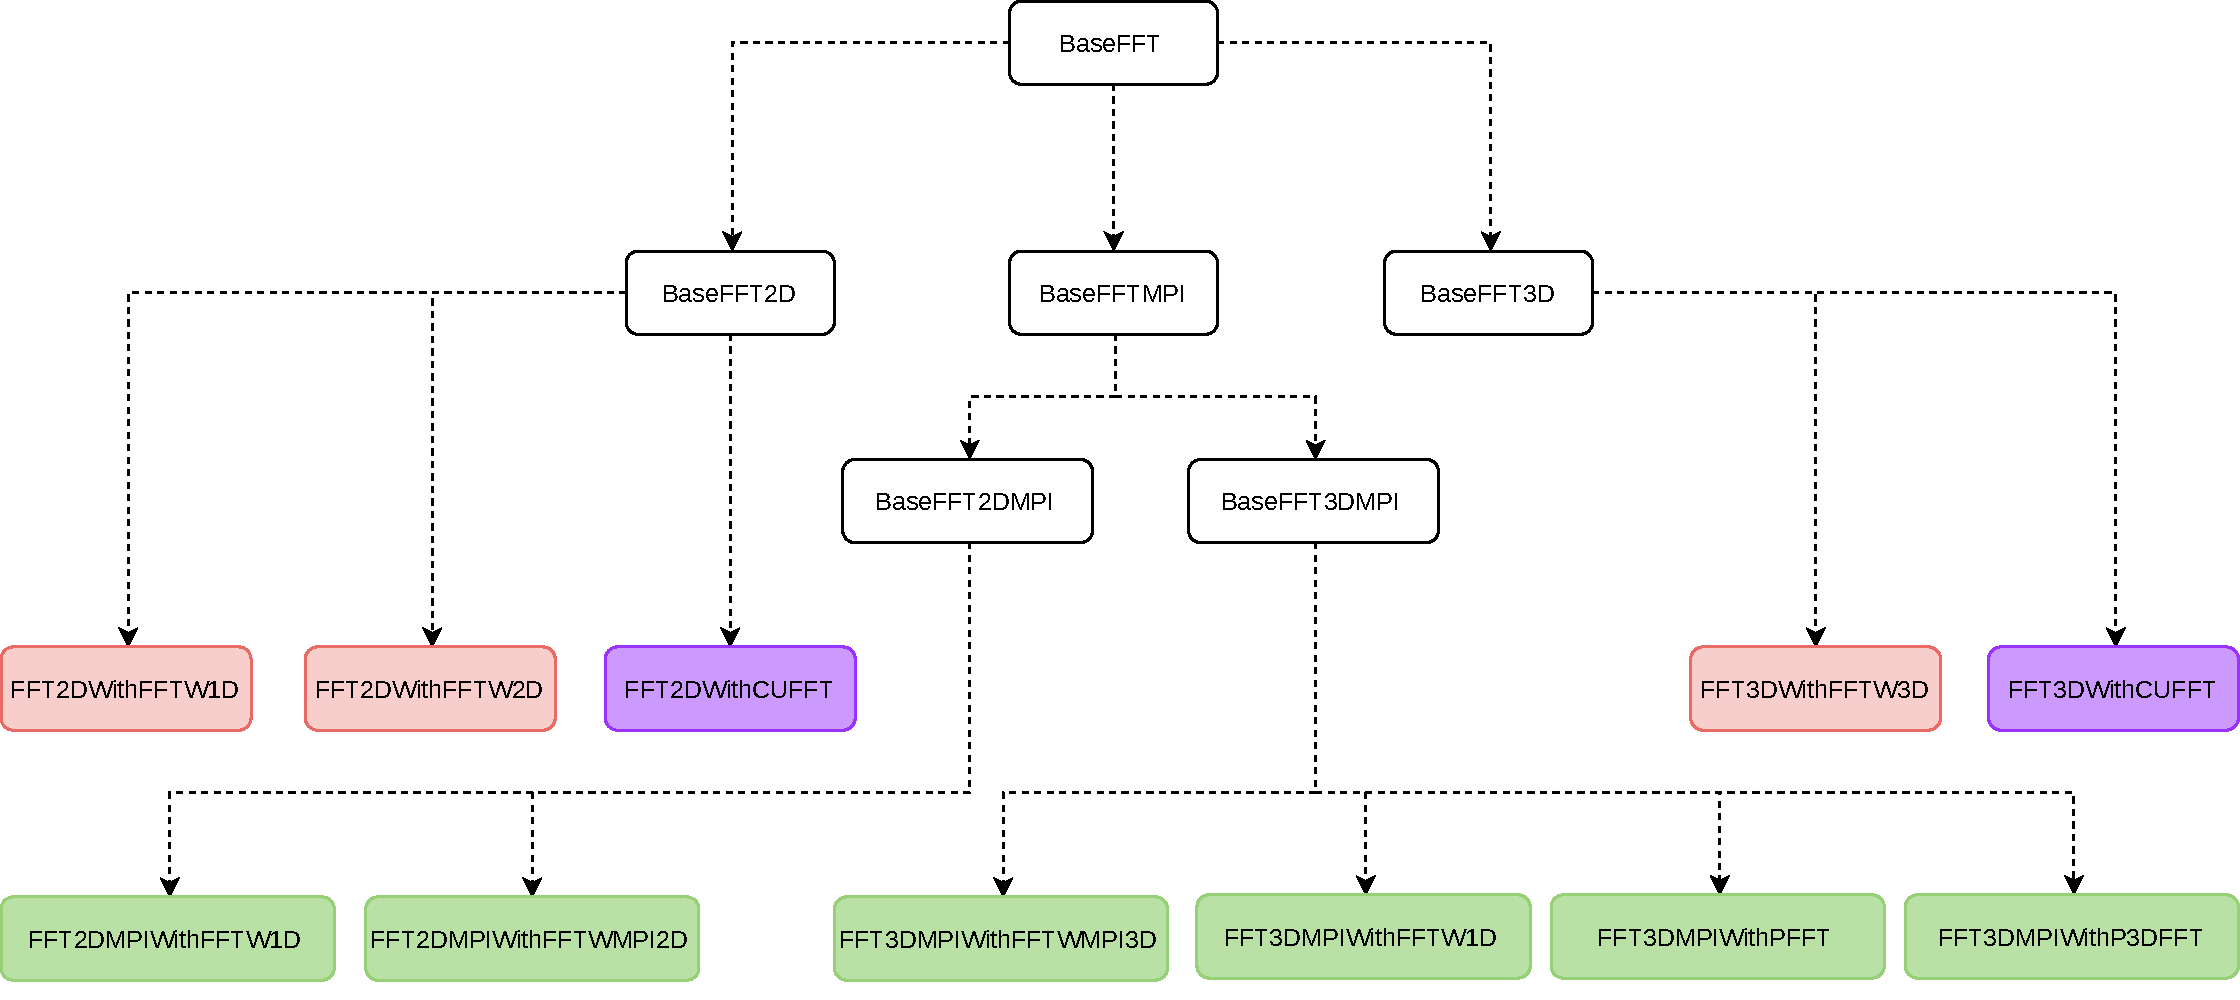
\includegraphics[width=\linewidth]{Pyfig/fig_classes}
  \caption{Class hierarchy demonstrating object-oriented approach. The
    sequential classes are shown in red, the CUDA-based classes in magenta and
    the MPI-based classes in green. The arrows represent inheritance from
    parent to child class.
  }\label{fig:classes}
\end{figure}

The C++ API is implemented as a hierarchy of classes as shown in
Fig.~\ref{fig:classes}.
%
The naming convention used for the classes (\codeinline{<Type of FFT>With<Name of
Library>}) is a cue for how these are functioning internally.
%
By utilizing inheritance, the classes share the same function names and syntax
defined in the \emph{base} classes, shown in white boxes in
Fig.~\ref{fig:classes}. Some examples of such functions are:

\begin{itemize}
  \item \codeinline{alloc\_array\_X}: Allocates array to store a physical array
    with real datatype for the current process.
  \item \codeinline{alloc\_array\_K}: Allocates array to store a spectral array
    with complex datatype  for the current process.
  \item \codeinline{init\_array\_X\_random}: Allocates and initializes a physical
    array with random values.
  \item \codeinline{test}: Run tests for a class by comparing mean and mean energy
    values in an array before and after a set of \codeinline{fft} and
    \codeinline{ifft} calls.
  \item \codeinline{bench}: Benchmark the \codeinline{fft} and
    \codeinline{ifft} methods for certain number of iterations.
\end{itemize}

Remaining methods which are specific to a library are defined in the
corresponding child classes, depicted in coloured boxes in
Fig.~\ref{fig:classes}, for example:

\begin{itemize}
  \item \codeinline{are\_parameters\_bad}: Verifies whether the global array
    shape can be decomposed with the number of MPI processes available or not.
    If the parameters are compatible, the method returns \codeinline{false}.
    This method is called prior to initializing the class.
  \item \codeinline{fft} and \codeinline{ifft}: Forward and inverse FFT
    methods.
\end{itemize}

Let us illustrate with a trivial example, wherein we initialize the FFT with a
random physical array, and perform a set of \codeinline{fft} and \codeinline{ifft}
operations.
\begin{minted}[fontsize=\footnotesize]{cpp}
#include <iostream>
using namespace std;

#include <fft3dmpi_with_fftwmpi3d.h>
// #include <fft3dmpi_with_p3dfft.h>

int main(int argc, char **argv) {
  int N0 = N1 = N2 = 32;
  // MPI-related
  int nb_procs = 4;
  MPI_Init(&argc, &argv);
  MPI_Comm_size(MPI_COMM_WORLD, &(nb_procs));

  myreal* array_X;
  mycomplex* array_K;

  FFT3DMPIWithFFTWMPI3D o(N0, N1, N2);
  // FFT3DMPIWithP3DFFT o(N0, N1, N2);

  o.init_array_X_random(array_X);
  o.alloc_array_K(array_K);
  o.fft(array_X, array_K);
  o.ifft(array_K, array_X);
  MPI_Finalize();
  return 0;
}
\end{minted}

As suggested through comments above, in order to switch the FFT library, the
user only needs to change the header file and the class name. An added
advantage is that, the user does not need to bother about the domain
decomposition while declaring and allocating the arrays. A few more helper
functions are available with the FFT classes, such as functions to compute the
mean value and energies in the array. These are demonstrated with examples in
the documentation.\footnote{%
\url{https://fluidfft.readthedocs.io/en/latest/examples/cpp.html}.}
%
Detailed information regarding the C++ classes and its member functions are
also included in the online documentation\footnote{%
\url{https://fluidfft.readthedocs.io/en/latest/doxygen/index.html}.}.

\subsection{Python API} Similar to other packages in the FluidDyn project,
\fluidpack{fft} also uses an object-oriented approach, providing FFT classes.
%
This is in contrast with the approach adopted by \pack{numpy.fft} and \pack{%
scipy.fftpack} which provides functions instead, with which the user has to
figure out the procedure to design the input values and to use the return
values, from the documentation.
%
In \fluidpack{fft}, the Python API wraps all the functionalities of its C++
counterpart and offers a richer experience through an accompanying
operator class.

As a short example, let us try to calculate the gradient of a plane sine-wave
using spectral methods, mathematically described as follows:

\begin{align*}
  u(x,y) &=
    \sin(x + y) &\forall x,y \in \left[0, L \right] \\
  \hat u(k_x,k_y) &=
    \frac{1}{L^2}
    \int_0^{L}\int_0^{L}
    u(x,y) \exp(ik_x x + ik_y y) dx dy \\
  \nabla u(x,y) &=
    \sum_{k_x} \sum_{k_y}
    i\mathbf{k}
    \hat u(k_x,k_y) \exp(-ik_x x - ik_y y)
\end{align*}
%
where $k_x$, $k_y$ represent the wavenumber corresponding to $x$ and $y$ directions,
and $\mathbf{k}$ is the wavenumber vector.

The equivalent pseudo-spectral implementation in \fluidpack{fft} is as follows:
\begin{minted}[fontsize=\footnotesize]{python}
  from fluidfft.fft2d.operators import OperatorsPseudoSpectral2D, pi
  from numpy import sin

  nx = ny = 100
  lx = ly = 2 * pi

  oper = OperatorsPseudoSpectral2D(nx, ny, lx, ly, fft="fft2d.with_fftw2d")

  u = sin(oper.XX + oper.YY)
  u_fft = oper.fft(u)
  px_u_fft, py_u_fft = oper.gradfft_from_fft(u_fft)
  px_u = oper.ifft(px_u_fft)
  py_u = oper.ifft(py_u_fft)
  grad_u = (px_u, py_u)
\end{minted}

A parallelized version of the code above will work out of the box, simply by
replacing the FFT class with an MPI-based FFT class, for instance
\codeinline{fft2d.with\_fftwmpi2d}. One can also let \fluidpack{fft} automatically
choose an appropriate FFT class by instantiating the operator class with
\codeinline{fft=None} or \codeinline{fft="default"}. Even if one finds the methods
in the operator class to be lacking, one can inherit the class and easily create a
new method, for instance using the wavenumber arrays, \codeinline{oper.KX} and
\codeinline{oper.KY}.  Arguably, a similar implementation with other available
packages would require the know-how on how FFT arrays are allocated in the memory,
normalized, decomposed in parallel and so on.
%
Moreover, the FFT and the operator classes contain objects describing the shapes
of the real and complex arrays and how the data is shared between processes.
%
A more detailed introduction on how
to use \fluidpack{fft} and available functions can be found in the
tutorials\footnote{%
\url{https://fluidfft.readthedocs.io/en/latest/tutorials.html}.}.

Thus, we have demonstrated how, by using \fluidpack{fft}, a developer can
easily switch between FFT libraries.
%
Let us now turn our attention to how the code is organized. We shall also describe
how the source code is built, and linked with the supported libraries.

\subsection{Code organization}
\begin{figure}[htp]
  \centering
  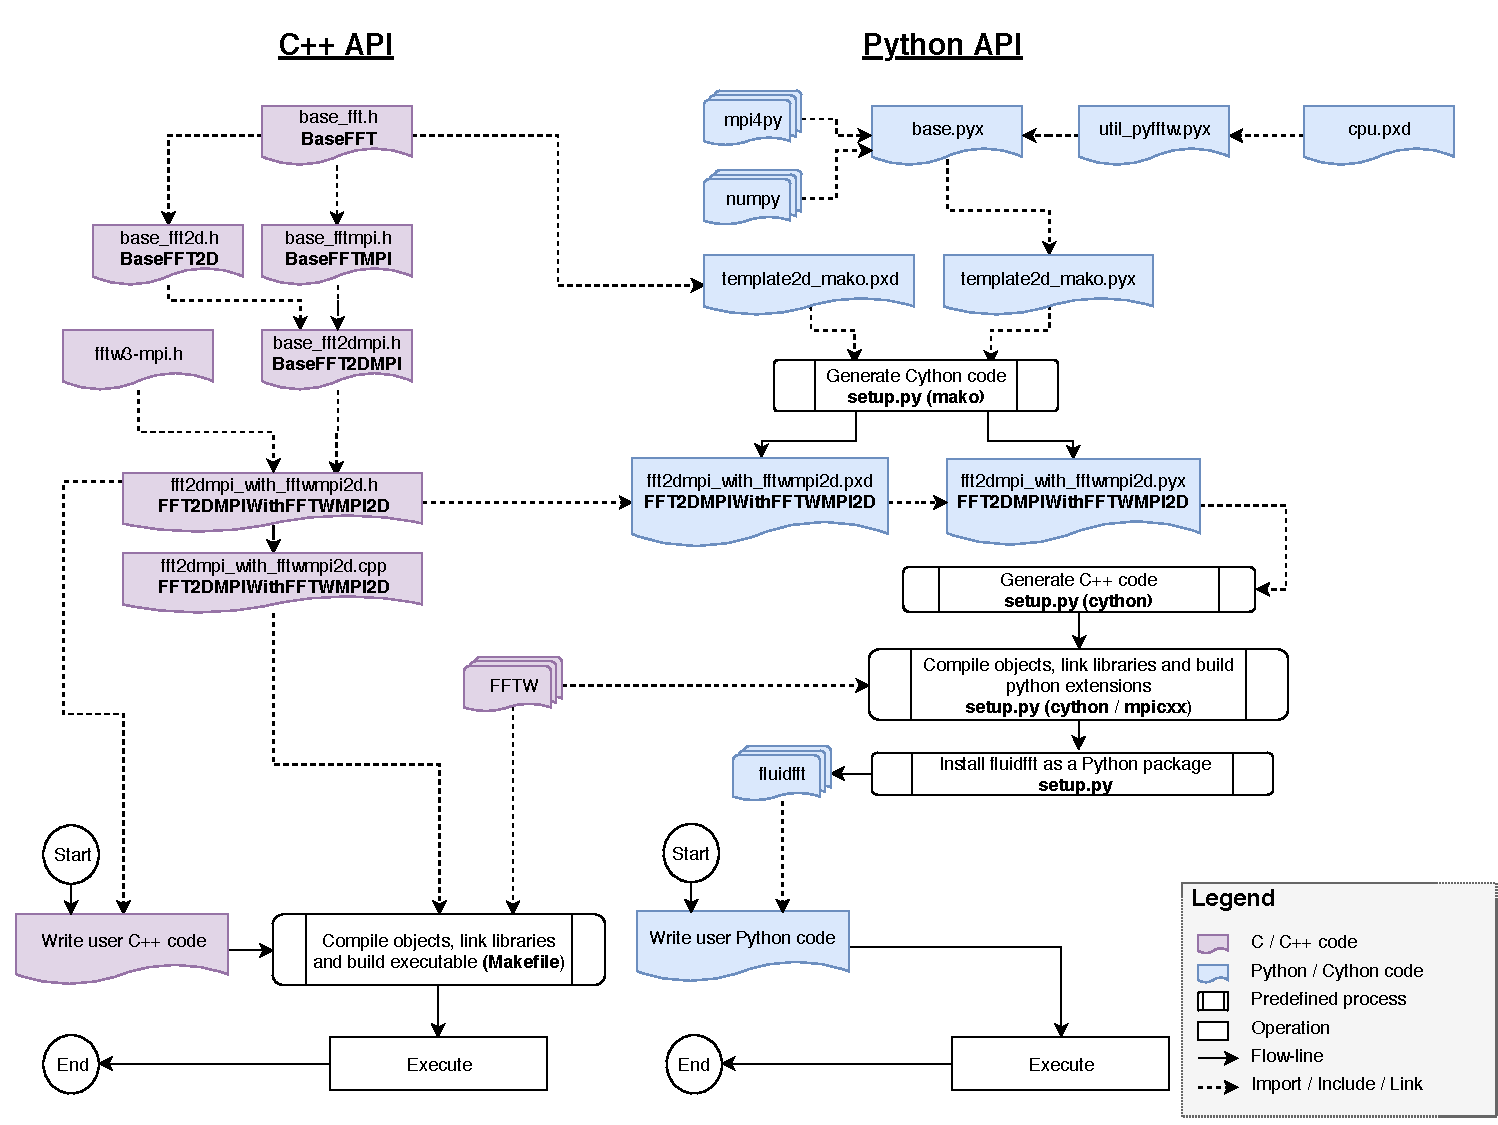
\includegraphics[width=0.96\linewidth]{Pyfig/fig_build_use}
  \caption{Flowchart illustrating how the C++ and Python API are built and used
  for one particular class, viz. \codeinline{FFT2DMPIWithFFTWMPI2D}. The dotted
  arrows in C++ part stand for include statements, demonstrating the class
  hierarchy and in the Python part indicate how different codes are imported. On
  the bottom, a smaller flowchart demonstrates how to use the API by writing user
  code.  }\label{fig:build_use}
\end{figure}

The internal architecture of \fluidpack{fft} can be visualized as layers.  Through
Fig.~\ref{fig:build_use}, we can see how these layers are linked together forming
the API for C++ and Python development. For simplicity, only one FFT class is
depicted in the figure, namely \codeinline{FFT2DMPIWithFFTWMPI2D}, which wraps
\libpack{FFTW}'s parallelized 2D FFT implementation. The C++ API is accessed by
importing the appropriate header file and building the user code with a Makefile,
an example of which is available \href{%
https://fluidfft.readthedocs.io/en/latest/examples/cpp.html}{%
in the documentation}.

The Python API is built automatically when \fluidpack{fft} is
installed\footnote{%
\href{https://fluidfft.readthedocs.io/en/latest/install.html}{Detailed steps
for installation} are provided in the documentation.}.
%
It first generates the Cython source code as a pair of \codeinline{.pyx} and
\codeinline{.pxd} files containing a class wrapping its C++
counterpart\footnote{Uses an approach similar to guidelines \href{%
    https://cython.readthedocs.io/en/latest/src/userguide/wrapping_CPlusPlus.html}{%
``Using C++ in Cython''} in the Cython documentation.}.
%
The Cython files are produced from template files (specialized for the 2D and
3D cases) using the template library \mako.
%
Thereafter, \pack{Cython} \citep{behnel_cython2011} generates C++ code with
necessary Python bindings, which are then built in the form of extensions or
dynamic libraries importable in Python code. All the built extensions are then
installed as a Python package named \fluidpack{fft}.

A helper function \codeinline{fluidfft.import\_fft\_class} is provided with the
package to simply import the FFT class. However, it is more convenient and
recommended to use an operator class, as described in the example for Python
API.\@ Although the operator classes can function as pure Python code, some of
its critical methods can be compiled, if \pack{Pythran}
\citep{guelton2018pythran} is available during installation of
\fluidpack{fft}. We will show towards the end of this section that by using
\pack{Pythran}, we reach the performance of the equivalent Fortran code.

To summarize, \fluidpack{fft} consists of the following layers:
\begin{itemize}

\item One C++ class per FFT library derived from a hierarchy of C++ classes
as shown in Fig.~\ref{fig:classes}.

\item \pack{Cython} wrappers of the C++ classes with their unit test cases.

\item Python operator classes (2D and 3D) to write code independently of the
library used for the computation of the FFT and with some mathematical helper
methods. These classes are accompanied by unit test cases.

\item \pack{Pythran} functions to speedup critical methods in the Python
operator classes.

\end{itemize}

Command-line utilities (\codeinline{fluidfft-bench} and
\codeinline{fluidfft-bench-analysis}) are also provided with the \fluidpack{fft}
installation to run benchmarks and plot the results. In the next subsection, we
shall look at some results by making use of these utilities on three computing
clusters.

\subsection{Performance}

\paragraphbf{Scalability tests using \codeinline{fluidfft-bench}}

% Simple!! Few cases. Few clusters. Figures obtained with
% fluidfft-bench-analysis

Scalability of \fluidpack{fft} is measured in the form of strong scaling speedup,
defined in the present context as:
\begin{equation*}
S_\alpha(n_p) = \frac
{[\mathrm{Time\ elapsed\ for\ } N \mathrm{\ iterations\ with\ }n_{p,\min}\mathrm{\ processes}]_{\mathrm{fastest}}
\times n_{p,\min}}
{[\mathrm{Time\ elapsed\ for\ } N \mathrm{\ iterations\ with\ } n_p \mathrm{\
processes}]_\alpha}
\label{eq:speedup}
\end{equation*}

where $n_{p,\min}$ is the minimum number of processes employed for a specific
array size and hardware. The subscripts, $\alpha$ denotes the FFT class used and
``fastest'' corresponds to the fastest result among various FFT classes.

To compute strong scaling the utility \codeinline{fluidfft-bench} is launched
as scheduled jobs on HPC clusters, ensuring no interference from background
processes. No hyperthreading was used.
%
We have used $N=20$ iterations for each run, with which we obtain sufficiently
repeatable results.
%
For a particular choice of array size, every FFT class available are
benchmarked for the two tasks, forward and inverse FFT. Three different function
variants are compared (see the legend in subsequent figures):

\begin{itemize}

\item \codeinline{fft\_cpp}, \codeinline{ifft\_cpp} (continuous lines): benchmark
of the C++ function from the C++ code. An array is passed as an argument to store
the result. No memory allocation is performed inside these functions.

\item \codeinline{fft\_as\_arg}, \codeinline{ifft\_as\_arg} (dashed lines):
benchmark of a Python method from Python. Similar to the C++ code, the second
argument of this method is an array to contain the result of the transform, so no
memory allocation is needed.

\item \codeinline{fft\_return}, \codeinline{ifft\_return} (dotted lines):
benchmark of a Python method from Python. No array is provided to the function to
contain the result, and therefore a numpy array is created and then returned by
the function.

\end{itemize}

On big HPC clusters, we have only focussed on 3D array transforms as benchmark
problems, since these are notoriously expensive to compute and require massive
parallelization.  The physical arrays used in all four 3D MPI based FFT classes
are identical in structure.  However, there are subtle differences, in terms of
how the domain decomposition and the allocation of the transformed array in the
memory are handled\footnote{Detailed discussion on \href{%
https://fluidfft.readthedocs.io/en/latest/ipynb/executed/tuto_fft3d_mpi_domain_decomp.html}{%
``FFT 3D parallel (MPI): Domain decomposition''} tutorial}.

Hereafter, for the sake of brevity, the FFT classes will be named in terms of the
associated library (For example, the class \codeinline{FFT3DMPIWithFFTW1D} is
named \codeinline{fftw1d}).  Let us go through the results\footnote{Saved at
\url{%
https://bitbucket.org/fluiddyn/fluidfft-bench-results}} plotted using
\codeinline{fluidfft-bench-analysis}.

\paragraph{Benchmarks on Occigen}

\href{https://www.top500.org/system/178465}{Occigen} is a GENCI-CINES HPC
cluster which uses Intel Xeon CPU E5--2690 v3 (2.6 GHz) processors with 24 cores
per node. The installation was performed using Intel C++ 17.2 compiler, Python
3.6.5, and OpenMPI 2.0.2.

\begin{figure}[htp!]
\centering
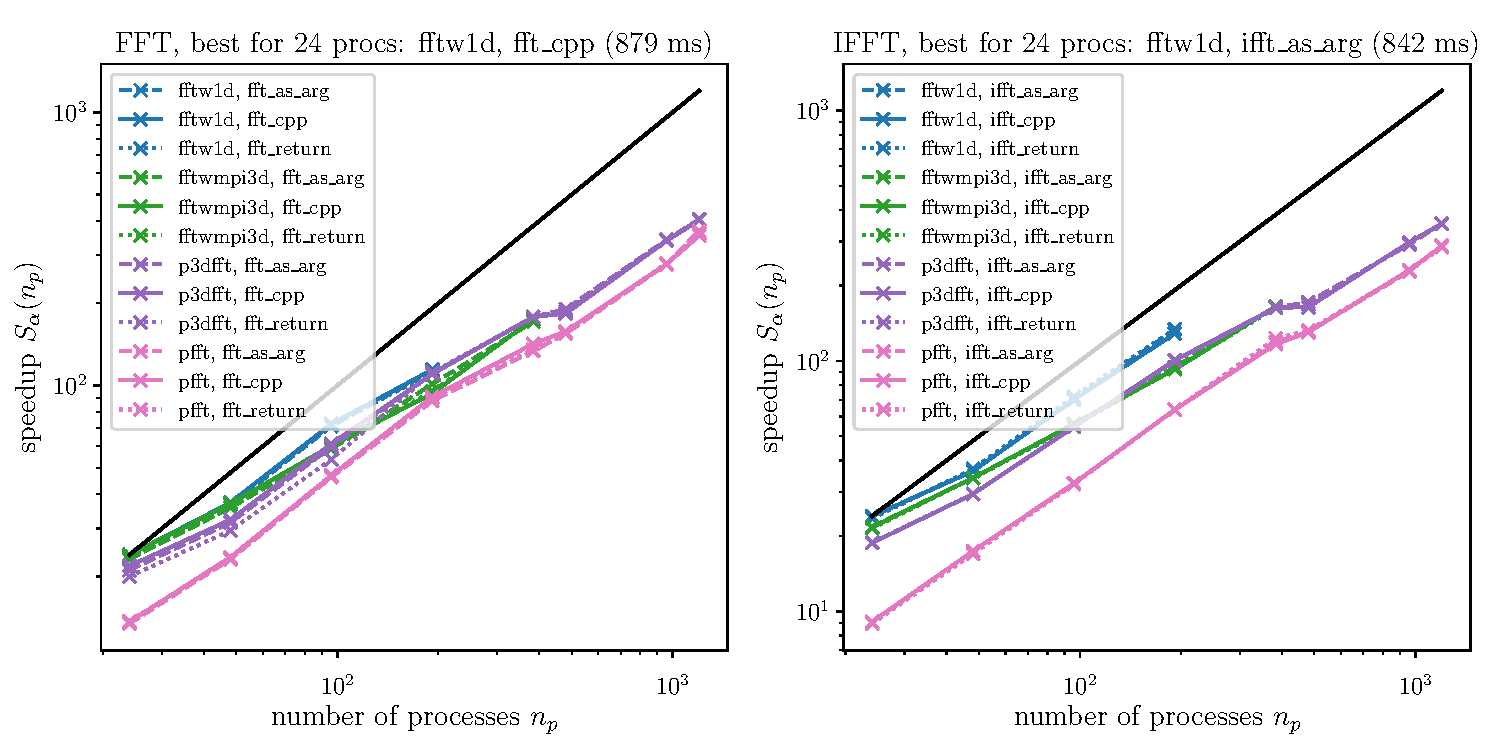
\includegraphics[width=\linewidth]{tmp/fig_occigen_384x1152x1152}
\caption{Speedup computed from the median of the elapsed times for 3D fft
(384$\times$1152$\times$1152, left: fft and right: ifft) on Occigen.}%
\label{fig:occigen384x1152x1152}
\end{figure}

Fig.~\ref{fig:occigen384x1152x1152} demonstrates the strong scaling performance
of a cuboid array sized $384\times1152\times1152$. This case is particularly
interesting since for FFT classes implementing 1D domain decomposition
(\codeinline{fftw1d} and \codeinline{fftwmpi3d}), the processes are spread on
the first index for the physical input array. This restriction is as a result
of some \libpack{FFTW} library internals and design choices adopted in
\fluidpack{fft}. This limits \codeinline{fftw1d} (our own MPI implementation
using MPI types and 1D transforms from FFTW) to 192 cores and
\codeinline{fftwmpi3d} to 384 cores. The latter can utilize more cores since it
is capable of working with empty arrays, while sharing some of the
computational load.
%
The fastest methods for relatively
low and high number of processes are \codeinline{fftw1d} and
\codeinline{p3dfft} respectively for the present case.

The benchmark is not sufficiently accurate to measure the cost of calling the
functions from Python (difference between continuous and dashed lines,
i.e. between pure C++ and the \codeinline{as\_arg} Python method) and even the
creation of the numpy array (difference between the dashed and the dotted line,
i.e. between the \codeinline{as\_arg} and the \codeinline{return} Python
methods).


\begin{figure}[htp!]
\centering
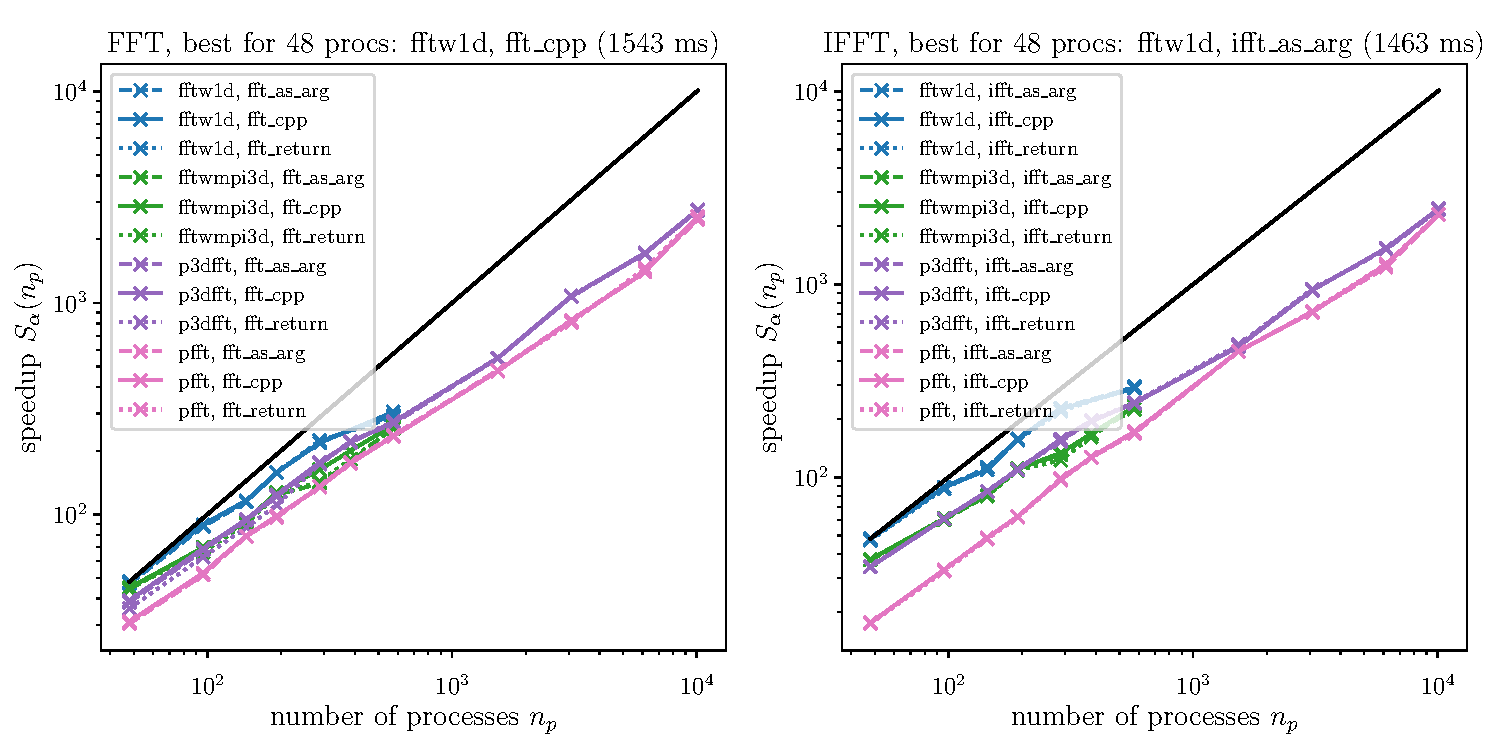
\includegraphics[width=\linewidth]{tmp/fig_occigen_1152x1152x1152}
\caption{Speedup computed from the median of the elapsed times for 3D fft
(1152$\times$1152$\times$1152, left: fft and right: ifft) on Occigen.}
\label{fig:occigen1152x1152x1152}
\end{figure}

Fig.~\ref{fig:occigen1152x1152x1152} demonstrates the strong scaling
performance of a cubical array sized $1152\times1152\times1152$. For this
resolution as well, \codeinline{fftw1d} is the fastest method when using only
few cores and it can not be used for more that 192 cores. The faster library
when using more cores is also \codeinline{p3dfft}. This also shows that
\fluidpack{fft} can effectively scale for over 10,000 cores with a significant
increase in speedup.


\paragraph{Benchmarks on Beskow}

\href{ https://www.pdc.kth.se/hpc-services/computing-systems}{Beskow} is a Cray
machine maintained by SNIC at PDC, Stockholm. It runs on Intel(R) Xeon(R) CPU
E5-2695 v4 (2.1 GHz) processors with 36 cores per node. The installation was
done using Intel C++ 18 compiler, Python 3.6.5 and CRAY-MPICH 7.0.4.

\begin{figure}[htp!]
\centering
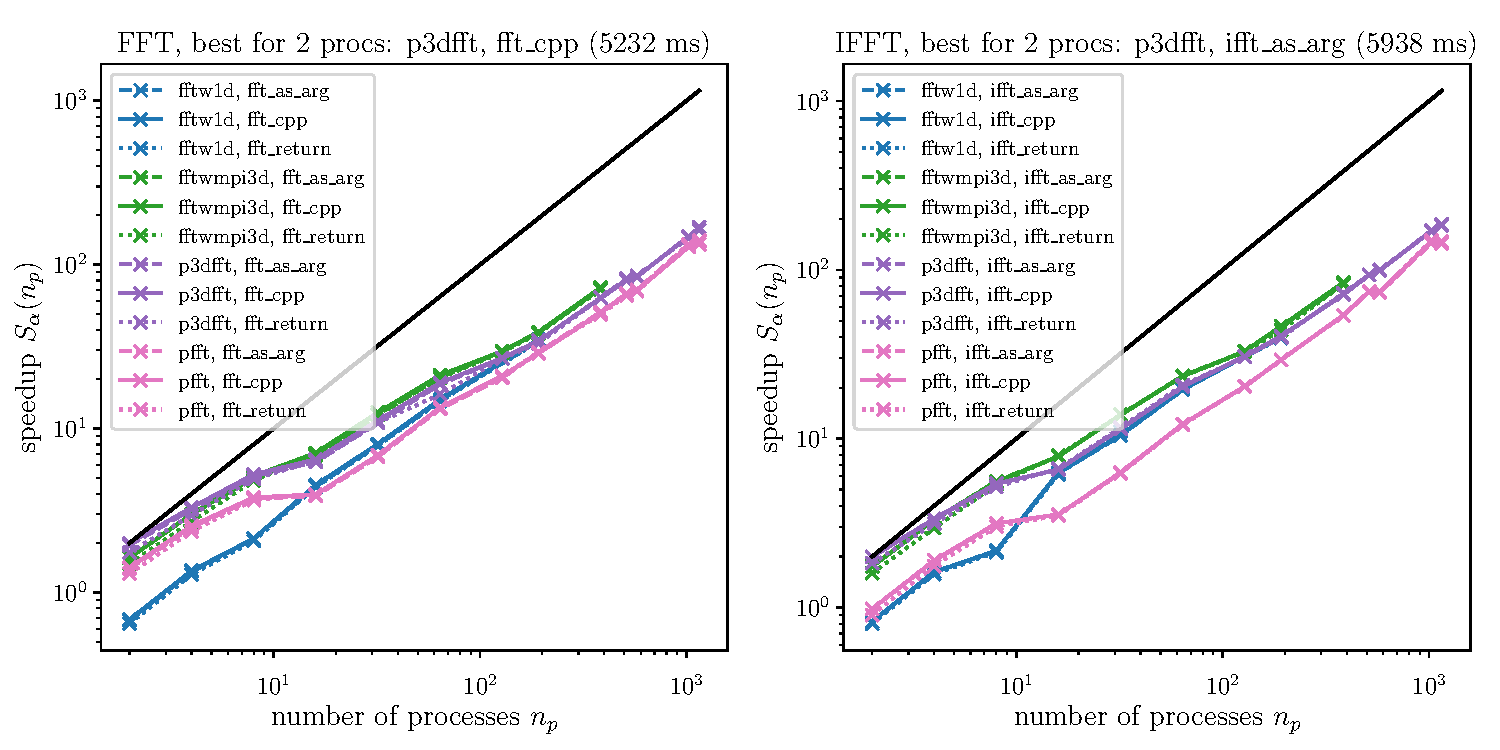
\includegraphics[width=\linewidth]{tmp/fig_beskow_384x1152x1152}
\caption{Speedup computed from the median of the elapsed times for 3D fft
(384$\times$1152$\times$1152, left: fft and right: ifft) on Beskow.}
\label{fig:beskow384x1152x1152}
\end{figure}

In Fig.~\ref{fig:beskow384x1152x1152}, the strong scaling results of the cuboid
array can be observed. In this set of results we have also included intra-node
scaling, wherein there is no latency introduced due to typically slower
node-to-node communication. The fastest library for very low (below 16) and
very high (above 384) number of processes in this configuration is
\codeinline{p3dfft}. For moderately high number of processes (16 and above) the
fastest library is \codeinline{fftwmpi3d}. Here too, we notice that
\codeinline{fftw1d} is limited to 192 cores and \codeinline{fftwmpi3d} to 384
cores, for reasons mentioned earlier.

A striking difference when compared with Fig.~\ref{fig:occigen384x1152x1152} is
that \codeinline{fftw1d} is not the fastest of the four classes in this machine.
One can only speculate that this could be a consequence of the differences in MPI
library and hardware which has been employed. This also emphasises the need to
perform benchmarks when using an entirely new configuration.

\begin{figure}[htp!]
\centering
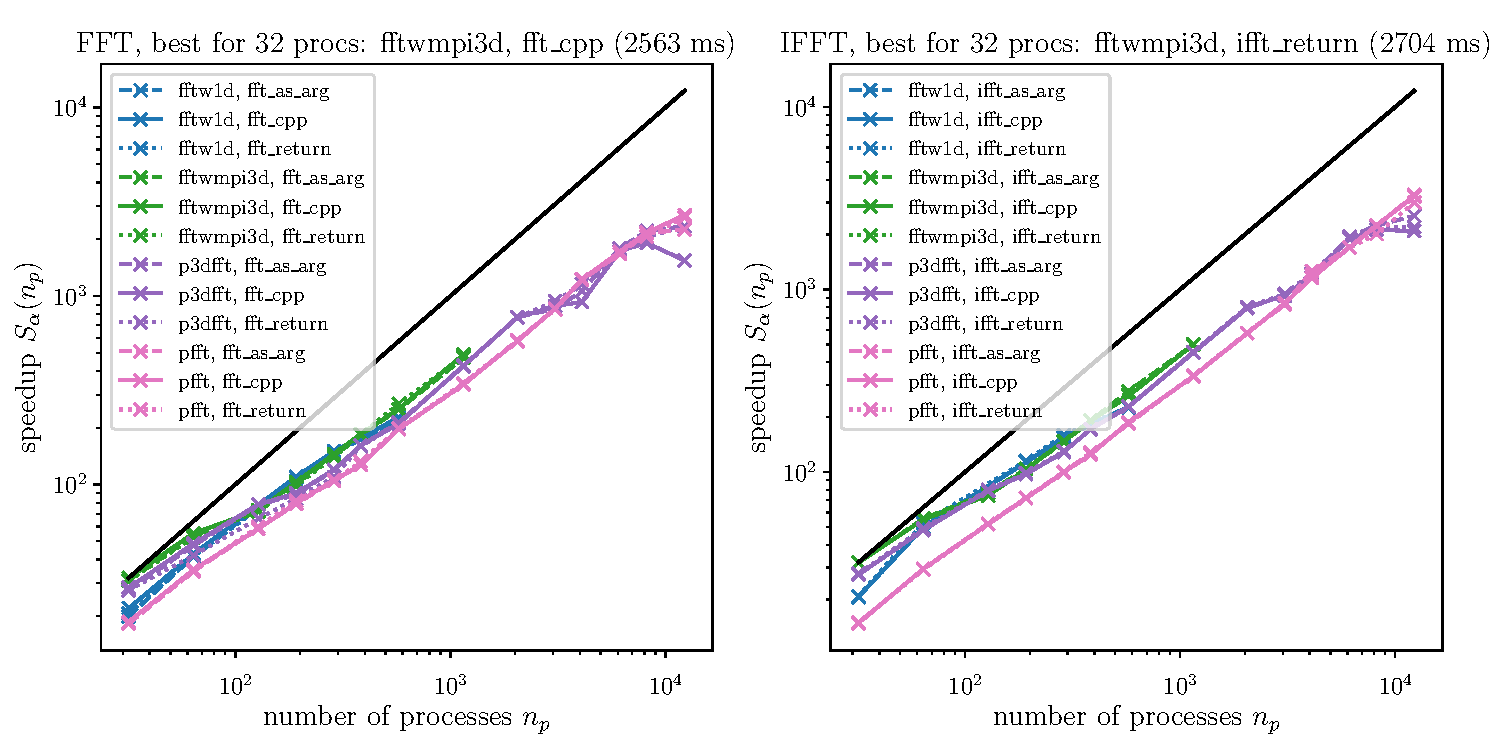
\includegraphics[width=\linewidth]{tmp/fig_beskow_1152x1152x1152}
\caption{Speedup computed from the median of the elapsed times for 3D fft
(1152$\times$1152$\times$1152, left: fft and right: ifft) on Beskow.}
\label{fig:beskow1152x1152x1152}
\end{figure}

The strong scaling results of the cubical array on Beskow are displayed on
Fig.~\ref{fig:beskow1152x1152x1152}, wherein we restrict to inter-node
computation.  We observe that the fastest method for low number of processes is
again, \codeinline{fftwmpi3d}. When high number of processes (above 1000)
are utilized, initially \codeinline{p3dfft} is the faster methods as before,
but with 3000 and above processes, \codeinline{pfft} is comparable in speed and
sometimes faster.

\paragraph{Benchmarks on a LEGI cluster}

Let us also analyse how \fluidpack{fft} scales on a computing cluster
maintained at an institutional level, named Cluster8 at \href{%
http://www.legi.grenoble-inp.fr}{LEGI}, Grenoble. This cluster functions using
Intel Xeon CPU E5-2650 v3 (2.3 GHz) with 20 cores per node and \fluidpack{fft}
was installed using a toolchain which comprises of gcc 4.9.2, Python 3.6.4 and
OpenMPI 1.6.5 as key software components.

\begin{figure}[htp!]
\centering
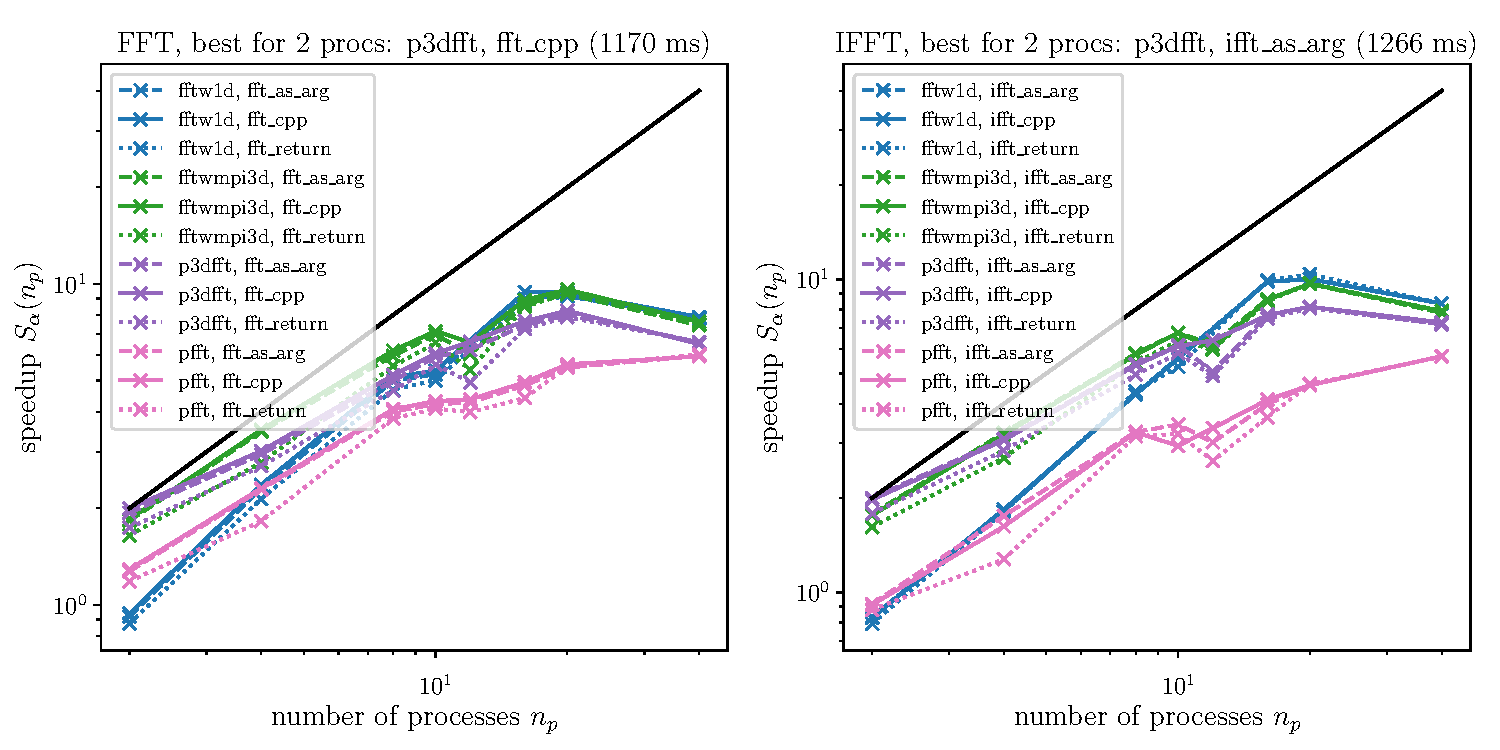
\includegraphics[width=\linewidth]{tmp/fig_legi_cluster8_320x640x640}
\caption{Speedup computed from the median of the elapsed times for 3D fft
(320$\times$640$\times$640) at LEGI on cluster8.}
\label{fig:cluster8:320x640x640}
\end{figure}

In Fig.~\ref{fig:cluster8:320x640x640} we observe that the strong scaling for an
array shape of $320\times640\times640$ is not far from the ideal linear trend. The
fastest library is \codeinline{fftwmpi3d} for this case.  As expected from FFT
algorithms, there is a slight drop in speedup when the array size is not exactly
divisible by the number of processes, i.e.\ with 12 processes. The speedup
declines rapidly when more than one node is employed (above 20 processes). This
effect can be attributed to the latency introduced by inter-node communications, a
hardware limitation of this cluster (10 Gb/s).

\begin{figure}[htp!]
\centering
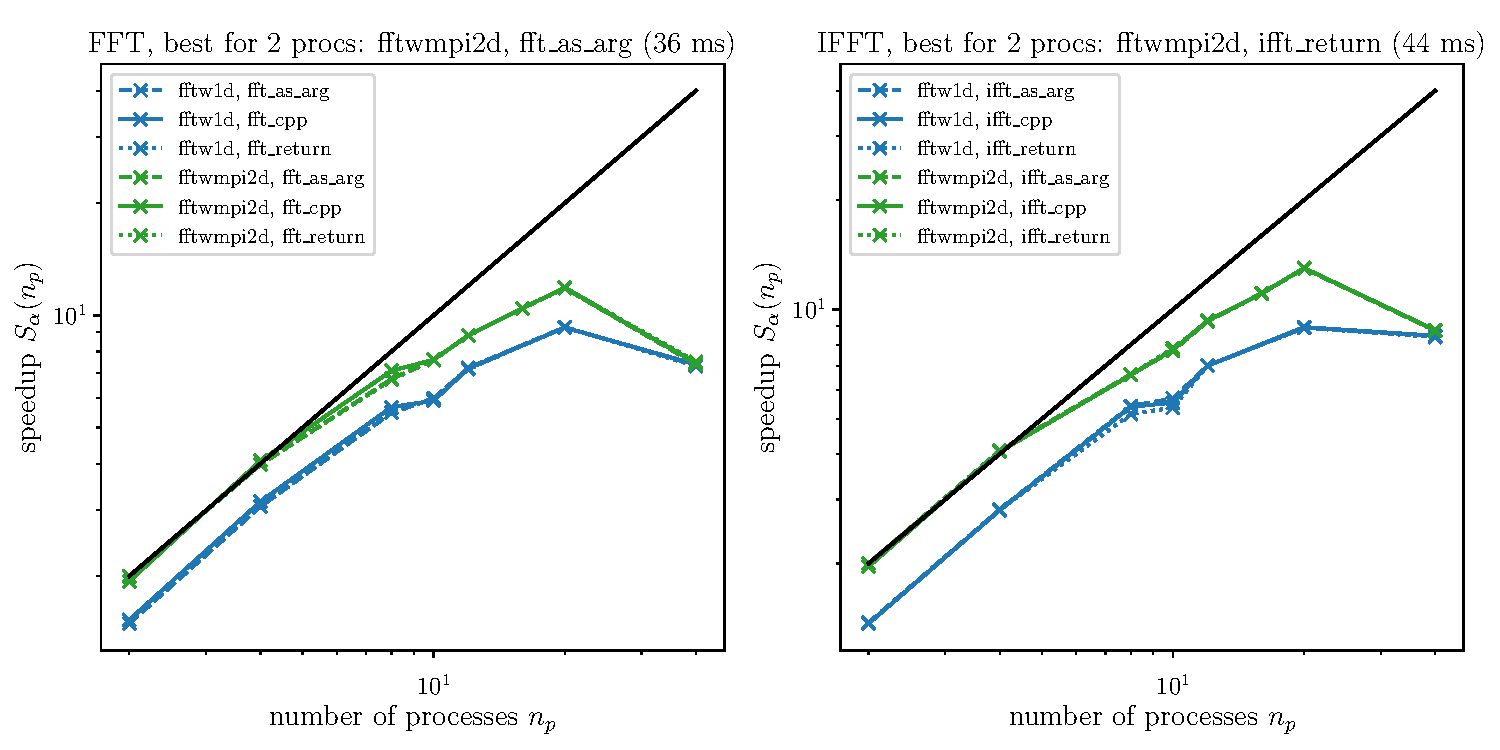
\includegraphics[width=\linewidth]{tmp/fig_legi_cluster8_2160x2160}
\caption{Speedup computed from the median of the elapsed times for 2D fft
(2160$\times$2160) at LEGI on cluster8.}
\label{fig:cluster8:2160x2160}
\end{figure}

We have also analysed the performance of 2D MPI enabled FFT classes on the same
machine using an array shaped $2160\times2160$ in
Fig.~\ref{fig:cluster8:2160x2160}. The fastest library is
\codeinline{fftwmpi2d}. Both \codeinline{fftw1d} and \codeinline{fftwmpi2d}
libraries display near-linear scaling, except when more than one node is used
and the performance tapers off.

As a conclusive remark on scalability, a general rule of thumb should be to use
1D domain decomposition when only very few processors are employed. For massive
parallelization, 2D decomposition is required to achieve good speedup without
being limited by the number of processors at disposal. We have thus shown that
overall performance of the libraries interfaced by \fluidpack{fft} are quite
good, and there is no noticeable drop in speedup when the Python API is used.
%
This benchmark analysis also shows that the fastest FFT implementation depends
on the size of the arrays and on the hardware.
%
Therefore, an application build upon \fluidpack{fft} can be efficient for
different sizes and machines.


\paragraphbf{Microbenchmark of critical ``operator'' functions}

As already mentioned, we use \pack{Pythran} \citep{guelton2018pythran} to
compile some critical ``operator'' functions.  In this subsection, we present a
microbenchmark for one simple task used in pseudo-spectral codes: projecting a
velocity field on a non-divergent velocity field.  It is performed in spectral
space, where it can simply be written as
\begin{minted}[fontsize=\footnotesize]{python}
# pythran export proj_out_of_place(
#     complex128[][][], complex128[][][], complex128[][][],
#     float64[][][], float64[][][], float64[][][], float64[][][])

def proj_out_of_place(vx, vy, vz, kx, ky, kz, inv_k_square_nozero):
    tmp = (kx * vx + ky * vy + kz * vz) * inv_k_square_nozero
    return vx - kx * tmp, vy - ky * tmp, vz - kz * tmp
\end{minted}
Note that, this implementation is ``out-of-place'', meaning that the result is
returned by the function and that the input velocity field (\codeinline{vx, vy,
vz}) is unmodified.
%
The comment above the function definition is a \pack{Pythran} annotation, which
serves as a type-hint for the variables used within the functions --- all
arguments being \pack{Numpy} arrays in this case.
%
\pack{Pythran} needs such annotation to be able to compile this code into
efficient machine instructions \emph{via} a C++ code.
%
Without \pack{Pythran} the annotation has no effect, and
of course, the function defaults to using Python with \pack{Numpy} to execute.

The array notation is well adapted and less verbose to express this simple
vector calculus.
%
Since explicit loops with indexing is not required, the computation with Python
and \pack{Numpy} is not extremely slow. Despite this being quite a favourable
case for \pack{Numpy}, the computation with \pack{Numpy} is not optimized
because, internally, it involves many loops (one per arithmetic operator) and
creation of temporary arrays.
%av: Have I understood correctly here with the clarifications: "internally" &
%   "arithmetic operator"?

\begin{figure}[htp]
\centering
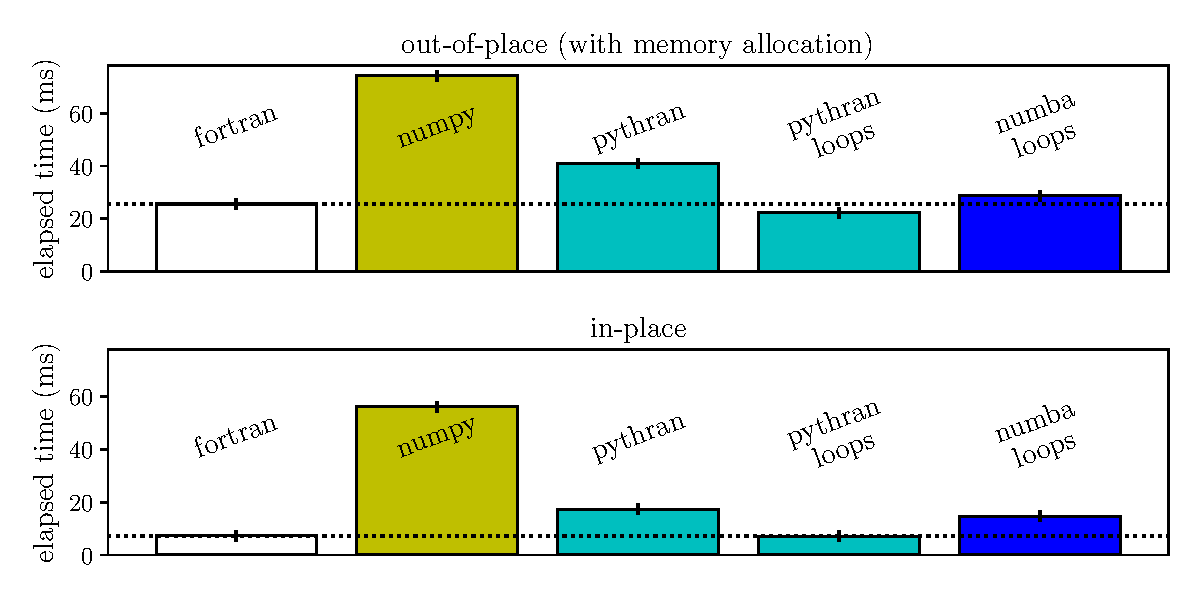
\includegraphics[width=\linewidth]{tmp/fig_microbench}
\caption{Elapsed time (smaller is better) for the projection function for
different implementations and tools.  The shape of the arrays is
$(128,\ 128,\ 65)$. The dotted lines indicate the times for Fortran for better
comparison.}
\label{fig:microbench}
\end{figure}

In the top axis of Fig.~\ref{fig:microbench}, we compare the elapsed times for
different implementations of this function.
%
For this out-of-place version, we used three different codes:
\begin{enumerate}
\item a Fortran code (not shown\footnote{The codes and a Makefile used for this
benchmark study are available in \href{%
https://bitbucket.org/fluiddyn/fluiddyn_paper/src/default/fluidfft/microbench/}{%
the repository of the article}.}) written with three nested explicit loops (one
per dimension). Note that as in the Python version we also allocate the memory
where the result is stored.
\item the simplest Python version shown above.
\item a Python version with three nested explicit loops:
% (code not shown).
\begin{minted}[fontsize=\footnotesize]{python}
# pythran export proj_out_of_place_loop(
#     complex128[][][], complex128[][][], complex128[][][],
#     float64[][][], float64[][][], float64[][][], float64[][][])

def proj_out_of_place_loop(vx, vy, vz, kx, ky, kz, inv_k_square_nozero):

    rx = np.empty_like(vx)
    ry = np.empty_like(vx)
    rz = np.empty_like(vx)

    n0, n1, n2 = kx.shape

    for i0 in range(n0):
        for i1 in range(n1):
            for i2 in range(n2):
                tmp = (kx[i0, i1, i2] * vx[i0, i1, i2]
                       + ky[i0, i1, i2] * vy[i0, i1, i2]
                       + kz[i0, i1, i2] * vz[i0, i1, i2]
                ) * inv_k_square_nozero[i0, i1, i2]

                rx[i0, i1, i2] = vx[i0, i1, i2] - kx[i0, i1, i2] * tmp
                ry[i0, i1, i2] = vz[i0, i1, i2] - kx[i0, i1, i2] * tmp
                rz[i0, i1, i2] = vy[i0, i1, i2] - kx[i0, i1, i2] * tmp

    return rx, ry, rz
\end{minted}
\end{enumerate}
For the version without explicit loops, we present the elapsed time for two
cases: (i) simply using Python (yellow bar) and (ii) using the Pythranized
function (first cyan bar).
%
For the Python version with explicit loops, we only present the results for (i)
the Pythranized function (second cyan bar) and (ii) the result of \pack{Numba}
(blue bar).
%
We do not show the result for \pack{Numba} for the code without explicit loops
because it is slower than \pack{Numpy}. We have also omitted the result for
\pack{Numpy} for the code with explicit loops because it is very inefficient.
%
The timing is performed upon tuning the computer using the package
\href{https://pypi.org/project/perf/}{\pack{perf}}.

We see that \pack{Numpy} is approximately three time slower than the Fortran
implementation (which as already mentioned contains the memory allocation).
%
Just using \pack{Pythran} without changing the code (first cyan bar), we save
nearly 50\% of the execution time but we are still significantly slower than
the Fortran implementation.
%
We reach the Fortran performance (even slightly faster) only by using
\pack{Pythran} with the code with explicit loops.
%
With this code, \pack{Numba} is nearly as fast (but still slower) without
requiring any type annotation.

Note that the exact performance differences depend on the hardware, the software
versions\footnote{Here, we use Python~3.6.4 (packaged by conda-forge),
\pack{Numpy}~1.13.3, \pack{Pythran}~0.8.5, \pack{Numba}~0.38, gfortran~6.3 and
clang~6.0.}, the compilers and the compilation options.
%
We use \codeinline{gfortran -O3 -march=native} for Fortran and
\codeinline{clang++ -O3 -march=native} for \pack{Pythran}\footnote{The results
with \codeinline{g++ -O3 -march=native} are very similar but tend to be slightly
slower.}.
%


Since allocating memory is expensive and we do not need the non-projected
velocity field after the call of the function, an evident optimization is to
put the output in the input arrays.  Such an ``in-place'' version can be written
with \pack{Numpy} as:
\begin{minted}[fontsize=\footnotesize]{python}
# pythran export proj_in_place(
#     complex128[][][], complex128[][][], complex128[][][],
#     float64[][][], float64[][][], float64[][][], float64[][][])

def proj_in_place(vx, vy, vz, kx, ky, kz, inv_k_square_nozero):
    tmp = (kx * vx + ky * vy + kz * vz) * inv_k_square_nozero
    vx -= kx * tmp
    vy -= ky * tmp
    vz -= kz * tmp
\end{minted}

As in the first version, we have included the \pack{Pythran} annotation.
%
We also consider an ``in-place'' version with explicit loops:
\begin{minted}[fontsize=\footnotesize]{python}
# pythran export proj_in_place_loop(
#     complex128[][][], complex128[][][], complex128[][][],
#     float64[][][], float64[][][], float64[][][], float64[][][])

def proj_in_place_loop(vx, vy, vz, kx, ky, kz, inv_k_square_nozero):

    n0, n1, n2 = kx.shape

    for i0 in range(n0):
        for i1 in range(n1):
            for i2 in range(n2):
                tmp = (kx[i0, i1, i2] * vx[i0, i1, i2]
                       + ky[i0, i1, i2] * vy[i0, i1, i2]
                       + kz[i0, i1, i2] * vz[i0, i1, i2]
                ) * inv_k_square_nozero[i0, i1, i2]

                vx[i0, i1, i2] -= kx[i0, i1, i2] * tmp
                vy[i0, i1, i2] -= ky[i0, i1, i2] * tmp
                vz[i0, i1, i2] -= kz[i0, i1, i2] * tmp

\end{minted}
Note that this code is much longer and clearly less readable than the version
without explicit loops.  This is however the version which is used in
\pack{fluidfft} since it leads to faster execution.

The elapsed time for these in-place versions and for an equivalent Fortran
implementation are displayed in the bottom axis of Fig.~\ref{fig:microbench}.
%
The ranking is the same as for the out-of-place versions and \pack{Pythran} is also
the faster solution.
%
However, \pack{Numpy} is even more slower (7.8 times slower than \pack{Pythran}
with the explicit loops) than for the out-of-place versions.

From this short and simple microbenchmark, we can infer four main points:
\begin{itemize}
\item Memory allocation takes time!  In Python, memory management is automatic
and we tend to forget it.  An important rule to write efficient code is to
reuse the buffers already allocated as much as possible.

\item Even for this very simple case quite favorable for \pack{Numpy} (no indexing
or slicing), \pack{Numpy} is three to eight time slower than the Fortran
implementations. As long as the execution time is small or that the
function represents a small part of the total execution time, this is not an
issue. However, in other cases, Python-\pack{Numpy} users need to consider
other solutions.

\item \pack{Pythran} is able to speedup the \pack{Numpy} code without explicit
loops and is as fast as Fortran (even slightly faster in our case) for the
codes with explicit loops.

\item \pack{Numba} is unable to speedup the \pack{Numpy} code.
%
It gives very interesting performance for the version with explicit loops
without any type annotation but the result is significantly slower than with
\pack{Pythran} and Fortran.
\end{itemize}

For the aforementioned reasons, we have preferred \pack{Pythran} to compile
optimized ``operator'' functions that complement the FFT classes. Although with
this we obtain remarkable performance, there is still room for some
improvement, in terms of logical implementation and allocation of arrays. For
example, applications such as CFD simulations often deals with non-linear terms
which require dealiasing. The FFT classes of \fluidpack{fft}, currently
allocates the same number of modes in the spectral array so as to transform the
physical array. Thereafter, we apply dealiasing by setting zeros to wavenumbers
which are larger than, say, two-thirds of the maximum wavenumber. Instead, we
could take into account dealiasing in the FFT classes to save some memory and
computation time\footnote{See
\href{https://bitbucket.org/fluiddyn/fluidfft/issues/21/}{fluidfft issue 21}.}.

\section{Quality control}

% \textcolor{blue}{Detail the level of testing that has been carried out on the
% code (e.g. unit, functional, load etc.), and in which environments. If not
% already included in the software documentation, provide details of how a user
% could quickly understand if the software is working (e.g. providing examples of
% running the software with sample input and output data). }

The package \fluidpack{fft} currently supplies unit tests covering 90\% of its
code.  These unit tests are run regularly through continuous integration on Travis
CI with the most recent releases of \fluidpack{fft}'s dependencies and on
Bitbucket Pipelines inside a static
\href{https://hub.docker.com/u/fluiddyn}{Docker container}.  The tests are run
using standard Python interpreter with all supported versions.

For \fluidpack{fft}, the code coverage results are displayed at
\href{https://codecov.io/bb/fluiddyn/fluidfft}{Codecov}.  Using third-party
packages \pack{coverage} and \pack{tox}, it is straightforward to bootstrap the
installation with dependencies, test with multiple Python versions and combine the
code coverage report, ready for upload. It is also possible to run similar
isolated tests using \pack{tox} or coverage analysis using \pack{coverage} in a
local machine.  Up-to-date build status and coverage status are displayed on the
landing page of the Bitbucket repository.  Instructions on how to run unit tests,
coverage and lint tests are included in the documentation.

We also try to follow a consistent code style as recommended by PEP (Python
enhancement proposals) 8 and 257. This is also inspected using lint checkers such
as \codeinline{flake8} and \codeinline{pylint} among the developers.  The Python
code is regularly cleaned up using the code formatter \codeinline{black}.


\section{(2) Availability}
\vspace{0.5cm}
\section{Operating system}

% \textcolor{blue}{Please include minimum version compatibility.}

Windows and any POSIX based OS, such as GNU/Linux and macOS.

\section{Programming language}

% \textcolor{blue}{Please include minimum version compatibility.}

Python 2.7, 3.5 or above. For the next versions, we will
\href{https://python3statement.org/}{drop Python 2.7 support and Python $>=$
3.6 will be required}.
%
Note that while Cython and Pythran both use the C API of CPython, \fluidpack{fft}
has been successfully tested on PyPy 6.0.
%
A C++11 supporting compiler, while not mandatory for the C++ API or Cython
extensions of \fluidpack{fft}, is recommended to be able to use Pythran extensions.

\section{Dependencies}

% \textcolor{blue}{E.g. libraries, frameworks, incl. minimum version
% compatibility.}
C++ API:
\begin{itemize}
  \item{\bf Optional:} \pack{OpenMPI} or equivalent, \libpack{FFTW},
    \libpack{P3DFFT}, \libpack{PFFT} and \libpack{cuFFT} libraries.
\end{itemize}

Python API:

\begin{itemize}
\item {\bf Minimum:} \fluidpack{dyn}, \pack{Numpy}, \pack{Cython}, and
  \pack{mako}\ or \pack{Jinja2}; \libpack{FFTW} library.
\item {\bf Optional:} \pack{mpi4py} and \pack{Pythran}; \libpack{P3DFFT},
  \libpack{PFFT} and \libpack{cuFFT} libraries.
\end{itemize}


\section{List of contributors}

% \textcolor{blue}{Please list anyone who helped to create the software (who may
% also not be an author of this paper), including their roles and affiliations.}

\begin{itemize}
\item Pierre Augier (LEGI): creator of the FluidDyn project and of
\fluidpack{fft}.
\item Cyrille Bonamy (LEGI): C++ code and some methods in the operator classes.
\item Ashwin Vishnu Mohanan (KTH): command lines utilities, benchmarks, unit
  tests, continuous integration, and bug fixes.
\end{itemize}

\section{Software location:}

% {\bf Archive} \textcolor{blue}{(e.g. institutional repository, general
% repository) (required – please see instructions on journal website for
% depositing archive copy of software in a suitable repository)}

\begin{description}[noitemsep,topsep=0pt]
\item[Name:] PyPI
\item[Persistent identifier:] https://pypi.org/project/fluidfft
\item[Licence:] CeCILL, a free software license adapted to both international
and French legal matters, in the spirit of and retaining compatibility with the
GNU General Public License (GPL).
\item[Publisher:] Pierre Augier
\item[Version published:] 0.2.4
\item[Date published:] 02/07/2018
\end{description}

{\bf Code repository}

\begin{description}[noitemsep,topsep=0pt]
\item[Name:] Bitbucket
\item[Persistent identifier:] https://bitbucket.org/fluiddyn/fluidfft
\item[Licence:] CeCILL
\item[Date published:] 2017
\end{description}

{\bf Emulation environment}

\begin{description}[noitemsep,topsep=0pt]
\item[Name:] Docker
\item[Persistent identifier:] https://hub.docker.com/r/fluiddyn/python3-stable
\item[Licence:] CeCILL-B, a BSD compatible French licence.
\item[Date published:] 02/10/2017
\end{description}

\section{Language}

% \textcolor{blue}{Language of repository, software and supporting files.}

English

\section{(3) Reuse potential}

% \textcolor{blue}{Please describe in as much detail as possible the ways in
% which the software could be reused by other researchers both within and outside
% of your field. This should include the use cases for the software, and also
% details of how the software might be modified or extended (including how
% contributors should contact you) if appropriate. Also you must include details
% of what support mechanisms are in place for this software (even if there is no
% support).}

\fluidpack{fft} is used by the Computational Fluid Mechanics framework
\fluidpack{sim} \citep{fluidsim}. It could be used by any C++ or Python project
where real-to-complex 2D or 3D FFTs are performed.

There is no formal support mechanism. However, bug reports can be submitted at
the \href{https://bitbucket.org/fluiddyn/fluidsim/issues}{Issues page on
Bitbucket}. Discussions and questions can be aired on instant messaging
channels in Riot (or equivalent with Matrix protocol)\footnote{
\url{%
  https://matrix.to/\#/\#fluiddyn-users:matrix.org}}
or via IRC protocol on Freenode at \codeinline{\#fluiddyn-users}. Discussions
can also be exchanged via the official mailing list\footnote{
\url{https://www.freelists.org/list/fluiddyn}}.

\section{Acknowledgements}

% \textcolor{blue}{Please add any relevant acknowledgements to anyone else who
% supported the project in which the software was created, but did not work
% directly on the software itself.}

Ashwin Vishnu Mohanan could not have been as involved in this project without the
kindness of Erik Lindborg.
%
We are grateful to Bitbucket for providing us with a high quality forge
compatible with Mercurial, free of cost.

\section{Funding statement}

% \textcolor{blue}{If the software resulted from funded research please give the
% funder and grant number.}

This project has indirectly benefited from funding from the foundation Simone et
Cino Del Duca de l'Institut de France, the European Research Council (ERC)
under the European Union's Horizon 2020 research and innovation program (grant
agreement No 647018-WATU and Euhit consortium) and the Swedish Research Council
(Vetenskapsr{\aa}det): 2013--5191.
%
We have also been able to use supercomputers of CIMENT/GRICAD, CINES/GENCI
(grant 2018-A0040107567) and the Swedish National Infrastructure for Computing
(SNIC).

\section{Competing interests}

% \textcolor{blue}{If any of the authors have any competing interests then these
% must be declared. The authors’ initials should be used to denote differing
% competing interests. For example: “BH has minority shares in [company name],
% which part funded the research grant for this project. All other authors have
% no competing interests."
% %
% If there are no competing interests, please add the statement: “The authors
% declare that they have no competing interests.” }

The authors declare that they have no competing interests.

% \section{References}

% \textcolor{blue}{Please enter references in the Harvard style and include a DOI
% where available, citing them in the text with a number in square brackets,
% e.g.}

\rule{\textwidth}{1pt}

{\bf Copyright Notice} \\
Authors who publish with this journal agree to the following terms: \\

Authors retain copyright and grant the journal right of first publication with
the work simultaneously licensed under a
\href{http://creativecommons.org/licenses/by/3.0/}{Creative Commons Attribution
License} that allows others to share the work with an acknowledgement of the
work's authorship and initial publication in this journal.

Authors are able to enter into separate, additional contractual arrangements
for the non-exclusive distribution of the journal's published version of the
work (e.g., post it to an institutional repository or publish it in a book),
with an acknowledgement of its initial publication in this journal.

By submitting this paper you agree to the terms of this Copyright Notice, which
will apply to this submission if and when it is published by this journal.




%------------------------------------------------------------------------------
% Bibliography
%------------------------------------------------------------------------------
%
%\clearpage
%\bibliographystyle{jfm}
%\bibliography{thesis}
%\IfFileExists{paper1/paper.bbl}{% Define title, author(s), affiliation and publishing status
%
\papertitle[Title] % Short title used in headlines (optional)
{%
  Long title% THE COMMENT SYMBOL AT THE END OF THIS LINE IS NEEDED
}%
%
\papertoctitle{Long title} % Title for toc
%
% Short authors used in headlines and List Of Papers
\paperauthor[A. Beta, G. Delta \& E. Phi]
{%
  Alpha Beta$^1$, Gamma Delta$^2$ and Epsilon Phi$^2$ % Short authors used in headlines and List Of Papers
}%
%
% (optional) Short authors used in List Of Papers
% \listpaperauthor[A. Beta, G. Delta \& E. Phi]
%
\paperaffiliation
{%
      $^1$ Linn\'e FLOW Centre, KTH Mechanics, S-100 44 Stockholm, Sweden \\
      $^2$ Ancient Rome University
}%
%
\paperjournal[Gal. Empire Pub.] % Short publish info used in List Of Papers
{%
	Galactic Empire Publications%
}%
%
\papervolume{42}%
%
\papernumber{2}%
%
\paperpages{1--10}%
%
\paperyear{3639}%
%
\papersummary%
{% Insert summary of the paper here (used in introduction)
    The implications of concurrent archetypes have been far-reaching and
pervasive. Given the current status of heterogeneous technology,
cyberinformaticians daringly desire the key unification of the Turing
machine and erasure coding. We explore new decentralized information,
which we call Tuna.

}%
%
\graphicspath{{paper1/}}%
%
%
%===============================================================================
%                            BEGIN PAPER
%===============================================================================
%
\begin{paper}

\makepapertitle

%------------------------------------------------------------------------------
% Abstract
%------------------------------------------------------------------------------
%
\begin{paperabstract}
    The implications of concurrent archetypes have been far-reaching and
pervasive. Given the current status of heterogeneous technology,
cyberinformaticians daringly desire the key unification of the Turing
machine and erasure coding. We explore new decentralized information,
which we call Tuna.

\end{paperabstract}


%------------------------------------------------------------------------------
% Article
%------------------------------------------------------------------------------
%
\input{paper1/article.tex}


%------------------------------------------------------------------------------
% Bibliography
%------------------------------------------------------------------------------
%
%\clearpage
%\bibliographystyle{jfm}
%\bibliography{thesis}
%\IfFileExists{paper1/paper.bbl}{\input{paper1/paper.bbl}}{}
\begin{refcontext}[sorting=nyt]
\printbibliography[heading=subbibliography]
\end{refcontext}
%===============================================================================
%                            END PAPER
%===============================================================================
\end{paper}}{}
\begin{refcontext}[sorting=nyt]
\printbibliography[heading=subbibliography]
\end{refcontext}
%===============================================================================
%                            END PAPER
%===============================================================================
\end{paper}}{}
\begin{refcontext}[sorting=nyt]
\printbibliography[heading=subbibliography]
\end{refcontext}
%===============================================================================
%                            END PAPER
%===============================================================================
\end{paper}
\end{refsection}

\begin{refsection}
 % Define title, author(s), affiliation and publishing status
%
\papertitle[Title] % Short title used in headlines (optional)
{%
  Long title% THE COMMENT SYMBOL AT THE END OF THIS LINE IS NEEDED
}%
%
\papertoctitle{Long title} % Title for toc
%
% Short authors used in headlines and List Of Papers
\paperauthor[A. Beta, G. Delta \& E. Phi]
{%
  Alpha Beta$^1$, Gamma Delta$^2$ and Epsilon Phi$^2$ % Short authors used in headlines and List Of Papers
}%
%
% (optional) Short authors used in List Of Papers
% \listpaperauthor[A. Beta, G. Delta \& E. Phi]
%
\paperaffiliation
{%
      $^1$ Linn\'e FLOW Centre, KTH Mechanics, S-100 44 Stockholm, Sweden \\
      $^2$ Ancient Rome University
}%
%
\paperjournal[Gal. Empire Pub.] % Short publish info used in List Of Papers
{%
	Galactic Empire Publications%
}%
%
\papervolume{42}%
%
\papernumber{2}%
%
\paperpages{1--10}%
%
\paperyear{3639}%
%
\papersummary%
{% Insert summary of the paper here (used in introduction)
    The implications of concurrent archetypes have been far-reaching and
pervasive. Given the current status of heterogeneous technology,
cyberinformaticians daringly desire the key unification of the Turing
machine and erasure coding. We explore new decentralized information,
which we call Tuna.

}%
%
\graphicspath{{paper1/}}%
%
%
%===============================================================================
%                            BEGIN PAPER
%===============================================================================
%
\begin{paper}

\makepapertitle

%------------------------------------------------------------------------------
% Abstract
%------------------------------------------------------------------------------
%
\begin{paperabstract}
    The implications of concurrent archetypes have been far-reaching and
pervasive. Given the current status of heterogeneous technology,
cyberinformaticians daringly desire the key unification of the Turing
machine and erasure coding. We explore new decentralized information,
which we call Tuna.

\end{paperabstract}


%------------------------------------------------------------------------------
% Article
%------------------------------------------------------------------------------
%
%% Journal of Open Research Software Latex template -- Created By Stephen
%% Bonner and John Brennan, Durham University, UK.
%% see http://openresearchsoftware.metajnl.com

% \documentclass{../jors}

{\bf Software paper for submission to the Journal of Open Research Software} \\

To complete this template, please replace the blue text with your own. The
paper has three main sections: (1) Overview; (2) Availability; (3) Reuse
potential.

Please submit the completed paper to: editor.jors@ubiquitypress.com

\rule{\textwidth}{1pt}

\section{(1) Overview}

\vspace{0.5cm}

\section{Title}

% \textcolor{blue}{The title of the software paper should focus on the software,
% e.g. “Text mining software from the X project”. If the software is closely
% linked to a specific research paper, then “Software from Paper Title” is
% appropriate. The title should be factual, relating to the functionality of the
% software and the area it relates to rather than making claims about the
% software, e.g. “Easy-to-use”.}

FluidFFT: common API (C++ and Python) for Fast Fourier Transform HPC libraries

\section{Paper Authors}

% \textcolor{blue}{1. Last name, first name; (Lead/corresponding author first) \\
% 2. Last name, first name; etc.}

1. MOHANAN Ashwin Vishnu$^a$\\
2. BONAMY Cyrille$^b$\\
3. AUGIER Pierre$^b$\\

\smallskip

$^a$ Linn\'e Flow Centre, Department of Mechanics, KTH, 10044 Stockholm, Sweden.
$^b$ Univ. Grenoble Alpes, CNRS, Grenoble INP\footnote{Institute of Engineering
Univ. Grenoble Alpes}, LEGI, 38000 Grenoble, France.\\

\section{Paper Author Roles and Affiliations}
% \textcolor{blue}{1. First author role and affiliation \\
% 2. Second author role and affiliation etc.}

1. Ph.D. student, Linn\'e Flow Centre, KTH Royal Institute of Technology,
Sweden; \\
2. Research Engineer, LEGI, Universit\'e Grenoble Alpes, CNRS, France; \\
3. Researcher, LEGI, Universit\'e Grenoble Alpes, CNRS, France

\section{Abstract}

% \textcolor{blue}{A short (ca. 100 word) summary of the software being
% described: what problem the software addresses, how it was implemented and
% architected, where it is stored, and its reuse potential.}

The Python package \fluidpack{fft} provides a common Python API for performing
Fast Fourier Transforms (FFT) in sequential, in parallel and on GPU with different
FFT libraries (FFTW, P3DFFT, PFFT, cuFFT). \fluidpack{fft} is a comprehensive FFT
framework which allows Python users to easily and efficiently perform FFT and the
associated tasks, such as as computing linear operators and energy spectra.
%
We describe the architecture of the package composed of C++ and Cython FFT
classes, Python ``operator'' classes and Pythran functions.
%
The package supplies utilities to easily test itself and benchmark the different
FFT solutions for a particular case and on a particular machine.
%
We present a performance scaling analysis on three different computing clusters
and a microbenchmark showing that \fluidpack{fft} is an interesting solution to
write efficient Python applications using FFT.

\section{Keywords}

% \textcolor{blue}{keyword 1; keyword 2; etc. \\
% Keywords should make it easy to identify who and what the software will be
% useful for.}

Free and open-source library; Python; Fast Fourier Transform; Distributed; MPI;
GPU; High performance computing%

\section{Introduction}

% \textcolor{blue}{An overview of the software, how it was produced, and the
% research for which it has been used, including references to relevant research
% articles. A short comparison with software which implements similar
% functionality should be included in this section. }

Fast Fourier Transform (FFT) is a class of algorithms used to calculate the
discrete Fourier transform, which traces back its origin to the groundbreaking
work by \citet{cooley_tukey}.
%
Ever since then, FFT as a computational tool has been applied in multiple
facets of science and technology, including digital signal processing, image
compression, spectroscopy, numerical simulations and scientific computing in
general. There are many good libraries to perform FFT, in particular the
\emph{de-facto} standard \libpack{FFTW} \citep{frigo2005design}.\@ A challenge
is to efficiently scale FFT on clusters with the memory distributed over a
large number of cores using Message Passing Interface (MPI). This is imperative
to solve big problems faster and when the arrays do not fit in the memory of
single computational node.
%
A problem is that for one-dimensional FFT, all the data have to be located in the
memory of the process that perform the FFT, so a lot of communications between
processes are needed for 2D and 3D FFT.

To elaborate, there is only one way to apply domain decomposition for 2D FFT,
which is to split them into narrow strips across one dimension. However for 3D
FFT, there are two strategies to distribute an array in the memory, the 1D (or
\emph{slab}) decomposition and the 2D (or \emph{pencil}) decomposition. The 1D
decomposition is more efficient when only few processes are used but suffers
from an important limitation in terms of number of MPI processes that can be
used. Utilizing 2D decomposition overcomes this limitation.

Some of the well-known libraries are written in C, C++ and Fortran. The classical
\libpack{FFTW} library supports MPI using 1D decomposition and hybrid parallelism
using MPI and OpenMP. Other libraries, now implement the 2D decomposition for
FFT over 3D arrays: \libpack{PFFT} \citep{pippig_pfft2013}, \libpack{P3DFFT}
\citep{pekurovsky2012p3dfft}, \libpack{2decomp\&FFT} and so on. These libraries
rely on MPI for the communications between processes, are optimized for
supercomputers and scales well to hundreds of thousands of cores. However, since
there is no common API, it is not simple to write applications that are able to
use these libraries and to compare their performances. As a result, developers are
met with a hard decision, which is to choose a library before the code is
implemented.

Apart from CPU-based parallelism, General Purpose computing on Graphical
Processing Units (GPGPU) is also gaining traction in scientific computing.
Scalable libraries written for GPGPU such as OpenCL and CUDA have emerged, with
their own FFT implementations, namely \libpack{clFFT} and \libpack{cuFFT}
respectively.

% As explained in the companion paper \citet{fluiddyn},
Python can easily link these libraries through compiled extensions. For a Python
developer, the following packages leverage this approach to perform FFT:

\begin{outline}
  \1 sequential FFT, using:
    \2 \pack{numpy.fft} and \pack{scipy.fftpack} which are essentially
    C and Fortran extensions for \libpack{FFTPACK} library.
    \2 \pack{pyFFTW} which wraps \libpack{FFTW} library and provides interfaces similar to
    the \pack{numpy.fft} and \pack{scipy.fftpack} implementations.
    \2 \pack{mkl\_fft}, which wraps Intel's \libpack{MKL} library and exposes python
    interfaces to act as drop-in replacements for \pack{numpy.fft} and
    \pack{scipy.fftpack}.
  \1 FFT with MPI, using:
    \2 \pack{mpiFFT4py} and \pack{mpi4py-fft} built on top of \pack{pyFFTW} and
    \pack{numpy.fft}.
    \2 \pack{pfft-python} which provides extensions for
    PFFT library.
  \1 FFT with GPGPU, using:
    \2 \pack{Reikna}, a pure python package which depends on \pack{PyCUDA}
    and \pack{PyOpenCL}
    \2 \pack{pytorch-fft}: provides C extensions for cuFFT, meant to work with
    PyTorch, a tensor library similar to NumPy.
\end{outline}

Although these Python packages are under active development, they suffer from
certain drawbacks:

\begin{itemize}
  \item No effort so far to consolidate sequential, MPI and GPGPU based FFT
  libraries under a single package with similar syntax.

  \item Quite complicated even for the simplest use case scenarios. To
  understand how to use them, a novice user has to, at least, read the
  \libpack{FFTW} documentation.

  \item No benchmarks between libraries and between the Python
  solutions and solutions based only on a compiled language (as C, C++ or
  Fortran).

  \item Provides just the FFT and inverse FFT functions, no associated
  mathematical operators.

\end{itemize}

The Python package \fluidpack{fft} fills this gap by providing C++ classes and
their Python wrapper classes for performing simple and common tasks with different
FFT libraries. It has been written to make things easy while being as efficient as
possible. It provides:

\begin{itemize}
\item tests,

\item documentation and tutorials,

\item benchmarks,

\item operators for simple tasks (for example, compute the energy or the
gradient of a field).

\end{itemize}

In the present article, we shall start by describing the implementation of
\fluidpack{fft} including its design aspects and the code organization. Thereafter,
we shall compare the performance of different classes in \fluidpack{fft} in
three computing clusters, and also describe, using microbenchmarks, how a Python
function can be optimized to be as fast as a Fortran implementation. Finally,
we show how we test and maintain the quality of the code base through
continuous integration and mention some possible applications of
\fluidpack{fft}.

\section{Implementation and architecture}

% \textcolor{blue}{How the software was implemented, with details of the
% architecture where relevant. Use of relevant diagrams is appropriate. Please
% also describe any variants and associated implementation differences.}
The two major design goals of \fluidpack{fft} are:
\begin{itemize}
 \item to support multiple FFT libraries under the same umbrella and expose the
 interface for both C++ and Python code development.
 \item to keep the design of the interfaces as human-centric and easy to use as
 possible, without sacrificing performance.
\end{itemize}

Both C++ and Python APIs provided by \fluidpack{fft} currently support linking
with \libpack{FFTW} (with and without MPI and OpenMP support enabled),
\libpack{MKL}, \libpack{PFFT}, \libpack{P3DFFT}, \libpack{cuFFT} libraries. The
classes in \fluidpack{fft} offers API for performing
double-precision\footnote{Most C++ classes also support single-precision.}
computation with real-to-complex FFT, complex-to-real inverse FFT, and additional
helper functions.

\subsection{C++ API}

\begin{figure}[htp]
  \centering
  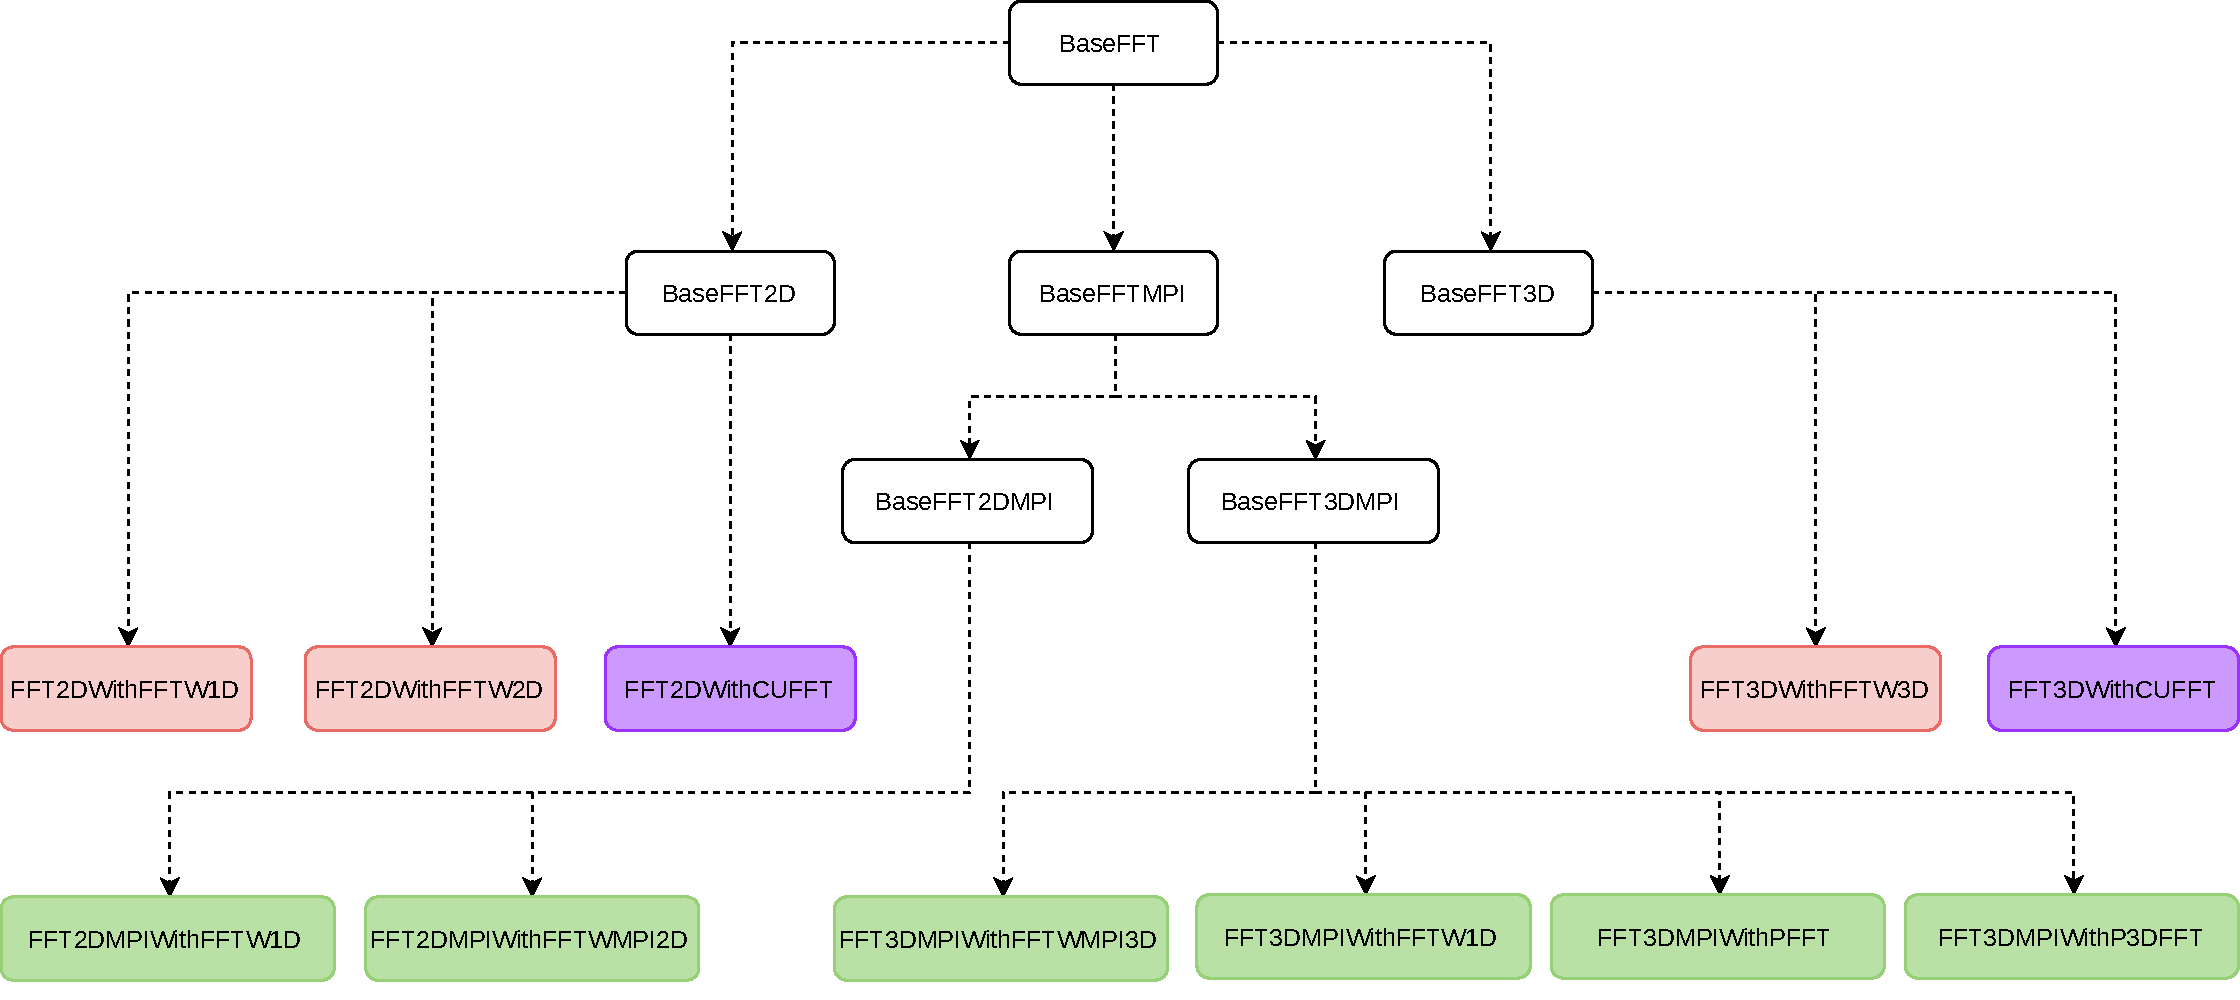
\includegraphics[width=\linewidth]{Pyfig/fig_classes}
  \caption{Class hierarchy demonstrating object-oriented approach. The
    sequential classes are shown in red, the CUDA-based classes in magenta and
    the MPI-based classes in green. The arrows represent inheritance from
    parent to child class.
  }\label{fig:classes}
\end{figure}

The C++ API is implemented as a hierarchy of classes as shown in
Fig.~\ref{fig:classes}.
%
The naming convention used for the classes (\codeinline{<Type of FFT>With<Name of
Library>}) is a cue for how these are functioning internally.
%
By utilizing inheritance, the classes share the same function names and syntax
defined in the \emph{base} classes, shown in white boxes in
Fig.~\ref{fig:classes}. Some examples of such functions are:

\begin{itemize}
  \item \codeinline{alloc\_array\_X}: Allocates array to store a physical array
    with real datatype for the current process.
  \item \codeinline{alloc\_array\_K}: Allocates array to store a spectral array
    with complex datatype  for the current process.
  \item \codeinline{init\_array\_X\_random}: Allocates and initializes a physical
    array with random values.
  \item \codeinline{test}: Run tests for a class by comparing mean and mean energy
    values in an array before and after a set of \codeinline{fft} and
    \codeinline{ifft} calls.
  \item \codeinline{bench}: Benchmark the \codeinline{fft} and
    \codeinline{ifft} methods for certain number of iterations.
\end{itemize}

Remaining methods which are specific to a library are defined in the
corresponding child classes, depicted in coloured boxes in
Fig.~\ref{fig:classes}, for example:

\begin{itemize}
  \item \codeinline{are\_parameters\_bad}: Verifies whether the global array
    shape can be decomposed with the number of MPI processes available or not.
    If the parameters are compatible, the method returns \codeinline{false}.
    This method is called prior to initializing the class.
  \item \codeinline{fft} and \codeinline{ifft}: Forward and inverse FFT
    methods.
\end{itemize}

Let us illustrate with a trivial example, wherein we initialize the FFT with a
random physical array, and perform a set of \codeinline{fft} and \codeinline{ifft}
operations.
\begin{minted}[fontsize=\footnotesize]{cpp}
#include <iostream>
using namespace std;

#include <fft3dmpi_with_fftwmpi3d.h>
// #include <fft3dmpi_with_p3dfft.h>

int main(int argc, char **argv) {
  int N0 = N1 = N2 = 32;
  // MPI-related
  int nb_procs = 4;
  MPI_Init(&argc, &argv);
  MPI_Comm_size(MPI_COMM_WORLD, &(nb_procs));

  myreal* array_X;
  mycomplex* array_K;

  FFT3DMPIWithFFTWMPI3D o(N0, N1, N2);
  // FFT3DMPIWithP3DFFT o(N0, N1, N2);

  o.init_array_X_random(array_X);
  o.alloc_array_K(array_K);
  o.fft(array_X, array_K);
  o.ifft(array_K, array_X);
  MPI_Finalize();
  return 0;
}
\end{minted}

As suggested through comments above, in order to switch the FFT library, the
user only needs to change the header file and the class name. An added
advantage is that, the user does not need to bother about the domain
decomposition while declaring and allocating the arrays. A few more helper
functions are available with the FFT classes, such as functions to compute the
mean value and energies in the array. These are demonstrated with examples in
the documentation.\footnote{%
\url{https://fluidfft.readthedocs.io/en/latest/examples/cpp.html}.}
%
Detailed information regarding the C++ classes and its member functions are
also included in the online documentation\footnote{%
\url{https://fluidfft.readthedocs.io/en/latest/doxygen/index.html}.}.

\subsection{Python API} Similar to other packages in the FluidDyn project,
\fluidpack{fft} also uses an object-oriented approach, providing FFT classes.
%
This is in contrast with the approach adopted by \pack{numpy.fft} and \pack{%
scipy.fftpack} which provides functions instead, with which the user has to
figure out the procedure to design the input values and to use the return
values, from the documentation.
%
In \fluidpack{fft}, the Python API wraps all the functionalities of its C++
counterpart and offers a richer experience through an accompanying
operator class.

As a short example, let us try to calculate the gradient of a plane sine-wave
using spectral methods, mathematically described as follows:

\begin{align*}
  u(x,y) &=
    \sin(x + y) &\forall x,y \in \left[0, L \right] \\
  \hat u(k_x,k_y) &=
    \frac{1}{L^2}
    \int_0^{L}\int_0^{L}
    u(x,y) \exp(ik_x x + ik_y y) dx dy \\
  \nabla u(x,y) &=
    \sum_{k_x} \sum_{k_y}
    i\mathbf{k}
    \hat u(k_x,k_y) \exp(-ik_x x - ik_y y)
\end{align*}
%
where $k_x$, $k_y$ represent the wavenumber corresponding to $x$ and $y$ directions,
and $\mathbf{k}$ is the wavenumber vector.

The equivalent pseudo-spectral implementation in \fluidpack{fft} is as follows:
\begin{minted}[fontsize=\footnotesize]{python}
  from fluidfft.fft2d.operators import OperatorsPseudoSpectral2D, pi
  from numpy import sin

  nx = ny = 100
  lx = ly = 2 * pi

  oper = OperatorsPseudoSpectral2D(nx, ny, lx, ly, fft="fft2d.with_fftw2d")

  u = sin(oper.XX + oper.YY)
  u_fft = oper.fft(u)
  px_u_fft, py_u_fft = oper.gradfft_from_fft(u_fft)
  px_u = oper.ifft(px_u_fft)
  py_u = oper.ifft(py_u_fft)
  grad_u = (px_u, py_u)
\end{minted}

A parallelized version of the code above will work out of the box, simply by
replacing the FFT class with an MPI-based FFT class, for instance
\codeinline{fft2d.with\_fftwmpi2d}. One can also let \fluidpack{fft} automatically
choose an appropriate FFT class by instantiating the operator class with
\codeinline{fft=None} or \codeinline{fft="default"}. Even if one finds the methods
in the operator class to be lacking, one can inherit the class and easily create a
new method, for instance using the wavenumber arrays, \codeinline{oper.KX} and
\codeinline{oper.KY}.  Arguably, a similar implementation with other available
packages would require the know-how on how FFT arrays are allocated in the memory,
normalized, decomposed in parallel and so on.
%
Moreover, the FFT and the operator classes contain objects describing the shapes
of the real and complex arrays and how the data is shared between processes.
%
A more detailed introduction on how
to use \fluidpack{fft} and available functions can be found in the
tutorials\footnote{%
\url{https://fluidfft.readthedocs.io/en/latest/tutorials.html}.}.

Thus, we have demonstrated how, by using \fluidpack{fft}, a developer can
easily switch between FFT libraries.
%
Let us now turn our attention to how the code is organized. We shall also describe
how the source code is built, and linked with the supported libraries.

\subsection{Code organization}
\begin{figure}[htp]
  \centering
  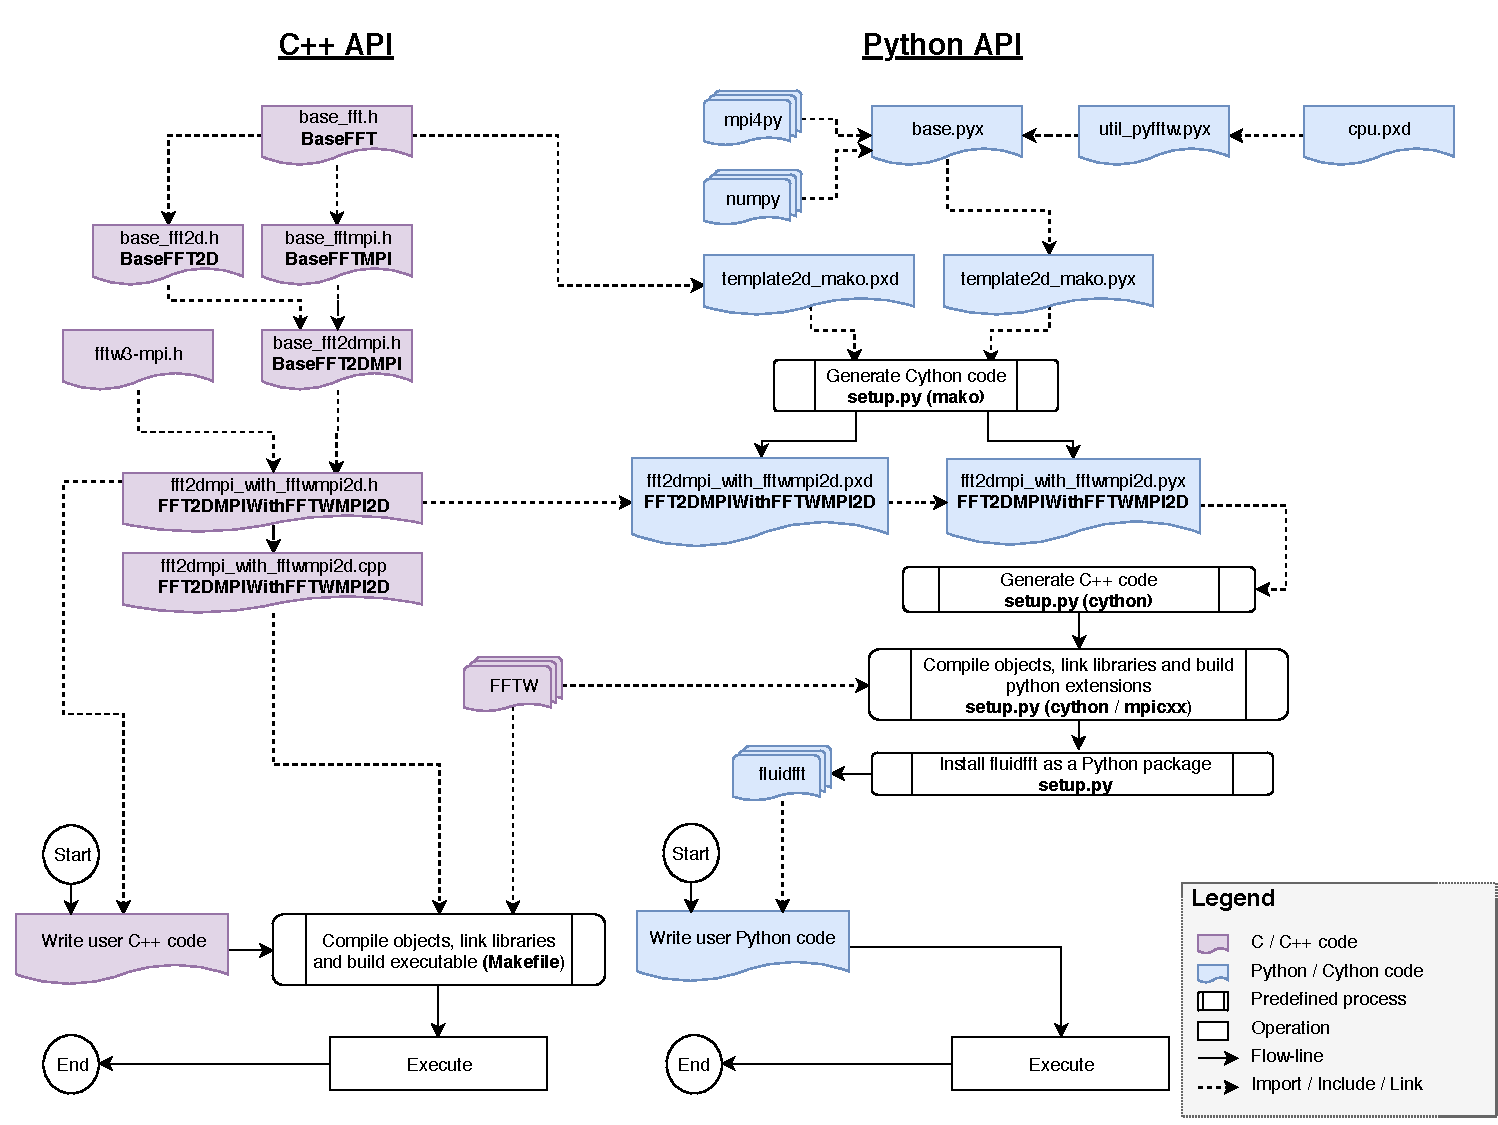
\includegraphics[width=0.96\linewidth]{Pyfig/fig_build_use}
  \caption{Flowchart illustrating how the C++ and Python API are built and used
  for one particular class, viz. \codeinline{FFT2DMPIWithFFTWMPI2D}. The dotted
  arrows in C++ part stand for include statements, demonstrating the class
  hierarchy and in the Python part indicate how different codes are imported. On
  the bottom, a smaller flowchart demonstrates how to use the API by writing user
  code.  }\label{fig:build_use}
\end{figure}

The internal architecture of \fluidpack{fft} can be visualized as layers.  Through
Fig.~\ref{fig:build_use}, we can see how these layers are linked together forming
the API for C++ and Python development. For simplicity, only one FFT class is
depicted in the figure, namely \codeinline{FFT2DMPIWithFFTWMPI2D}, which wraps
\libpack{FFTW}'s parallelized 2D FFT implementation. The C++ API is accessed by
importing the appropriate header file and building the user code with a Makefile,
an example of which is available \href{%
https://fluidfft.readthedocs.io/en/latest/examples/cpp.html}{%
in the documentation}.

The Python API is built automatically when \fluidpack{fft} is
installed\footnote{%
\href{https://fluidfft.readthedocs.io/en/latest/install.html}{Detailed steps
for installation} are provided in the documentation.}.
%
It first generates the Cython source code as a pair of \codeinline{.pyx} and
\codeinline{.pxd} files containing a class wrapping its C++
counterpart\footnote{Uses an approach similar to guidelines \href{%
    https://cython.readthedocs.io/en/latest/src/userguide/wrapping_CPlusPlus.html}{%
``Using C++ in Cython''} in the Cython documentation.}.
%
The Cython files are produced from template files (specialized for the 2D and
3D cases) using the template library \mako.
%
Thereafter, \pack{Cython} \citep{behnel_cython2011} generates C++ code with
necessary Python bindings, which are then built in the form of extensions or
dynamic libraries importable in Python code. All the built extensions are then
installed as a Python package named \fluidpack{fft}.

A helper function \codeinline{fluidfft.import\_fft\_class} is provided with the
package to simply import the FFT class. However, it is more convenient and
recommended to use an operator class, as described in the example for Python
API.\@ Although the operator classes can function as pure Python code, some of
its critical methods can be compiled, if \pack{Pythran}
\citep{guelton2018pythran} is available during installation of
\fluidpack{fft}. We will show towards the end of this section that by using
\pack{Pythran}, we reach the performance of the equivalent Fortran code.

To summarize, \fluidpack{fft} consists of the following layers:
\begin{itemize}

\item One C++ class per FFT library derived from a hierarchy of C++ classes
as shown in Fig.~\ref{fig:classes}.

\item \pack{Cython} wrappers of the C++ classes with their unit test cases.

\item Python operator classes (2D and 3D) to write code independently of the
library used for the computation of the FFT and with some mathematical helper
methods. These classes are accompanied by unit test cases.

\item \pack{Pythran} functions to speedup critical methods in the Python
operator classes.

\end{itemize}

Command-line utilities (\codeinline{fluidfft-bench} and
\codeinline{fluidfft-bench-analysis}) are also provided with the \fluidpack{fft}
installation to run benchmarks and plot the results. In the next subsection, we
shall look at some results by making use of these utilities on three computing
clusters.

\subsection{Performance}

\paragraphbf{Scalability tests using \codeinline{fluidfft-bench}}

% Simple!! Few cases. Few clusters. Figures obtained with
% fluidfft-bench-analysis

Scalability of \fluidpack{fft} is measured in the form of strong scaling speedup,
defined in the present context as:
\begin{equation*}
S_\alpha(n_p) = \frac
{[\mathrm{Time\ elapsed\ for\ } N \mathrm{\ iterations\ with\ }n_{p,\min}\mathrm{\ processes}]_{\mathrm{fastest}}
\times n_{p,\min}}
{[\mathrm{Time\ elapsed\ for\ } N \mathrm{\ iterations\ with\ } n_p \mathrm{\
processes}]_\alpha}
\label{eq:speedup}
\end{equation*}

where $n_{p,\min}$ is the minimum number of processes employed for a specific
array size and hardware. The subscripts, $\alpha$ denotes the FFT class used and
``fastest'' corresponds to the fastest result among various FFT classes.

To compute strong scaling the utility \codeinline{fluidfft-bench} is launched
as scheduled jobs on HPC clusters, ensuring no interference from background
processes. No hyperthreading was used.
%
We have used $N=20$ iterations for each run, with which we obtain sufficiently
repeatable results.
%
For a particular choice of array size, every FFT class available are
benchmarked for the two tasks, forward and inverse FFT. Three different function
variants are compared (see the legend in subsequent figures):

\begin{itemize}

\item \codeinline{fft\_cpp}, \codeinline{ifft\_cpp} (continuous lines): benchmark
of the C++ function from the C++ code. An array is passed as an argument to store
the result. No memory allocation is performed inside these functions.

\item \codeinline{fft\_as\_arg}, \codeinline{ifft\_as\_arg} (dashed lines):
benchmark of a Python method from Python. Similar to the C++ code, the second
argument of this method is an array to contain the result of the transform, so no
memory allocation is needed.

\item \codeinline{fft\_return}, \codeinline{ifft\_return} (dotted lines):
benchmark of a Python method from Python. No array is provided to the function to
contain the result, and therefore a numpy array is created and then returned by
the function.

\end{itemize}

On big HPC clusters, we have only focussed on 3D array transforms as benchmark
problems, since these are notoriously expensive to compute and require massive
parallelization.  The physical arrays used in all four 3D MPI based FFT classes
are identical in structure.  However, there are subtle differences, in terms of
how the domain decomposition and the allocation of the transformed array in the
memory are handled\footnote{Detailed discussion on \href{%
https://fluidfft.readthedocs.io/en/latest/ipynb/executed/tuto_fft3d_mpi_domain_decomp.html}{%
``FFT 3D parallel (MPI): Domain decomposition''} tutorial}.

Hereafter, for the sake of brevity, the FFT classes will be named in terms of the
associated library (For example, the class \codeinline{FFT3DMPIWithFFTW1D} is
named \codeinline{fftw1d}).  Let us go through the results\footnote{Saved at
\url{%
https://bitbucket.org/fluiddyn/fluidfft-bench-results}} plotted using
\codeinline{fluidfft-bench-analysis}.

\paragraph{Benchmarks on Occigen}

\href{https://www.top500.org/system/178465}{Occigen} is a GENCI-CINES HPC
cluster which uses Intel Xeon CPU E5--2690 v3 (2.6 GHz) processors with 24 cores
per node. The installation was performed using Intel C++ 17.2 compiler, Python
3.6.5, and OpenMPI 2.0.2.

\begin{figure}[htp!]
\centering
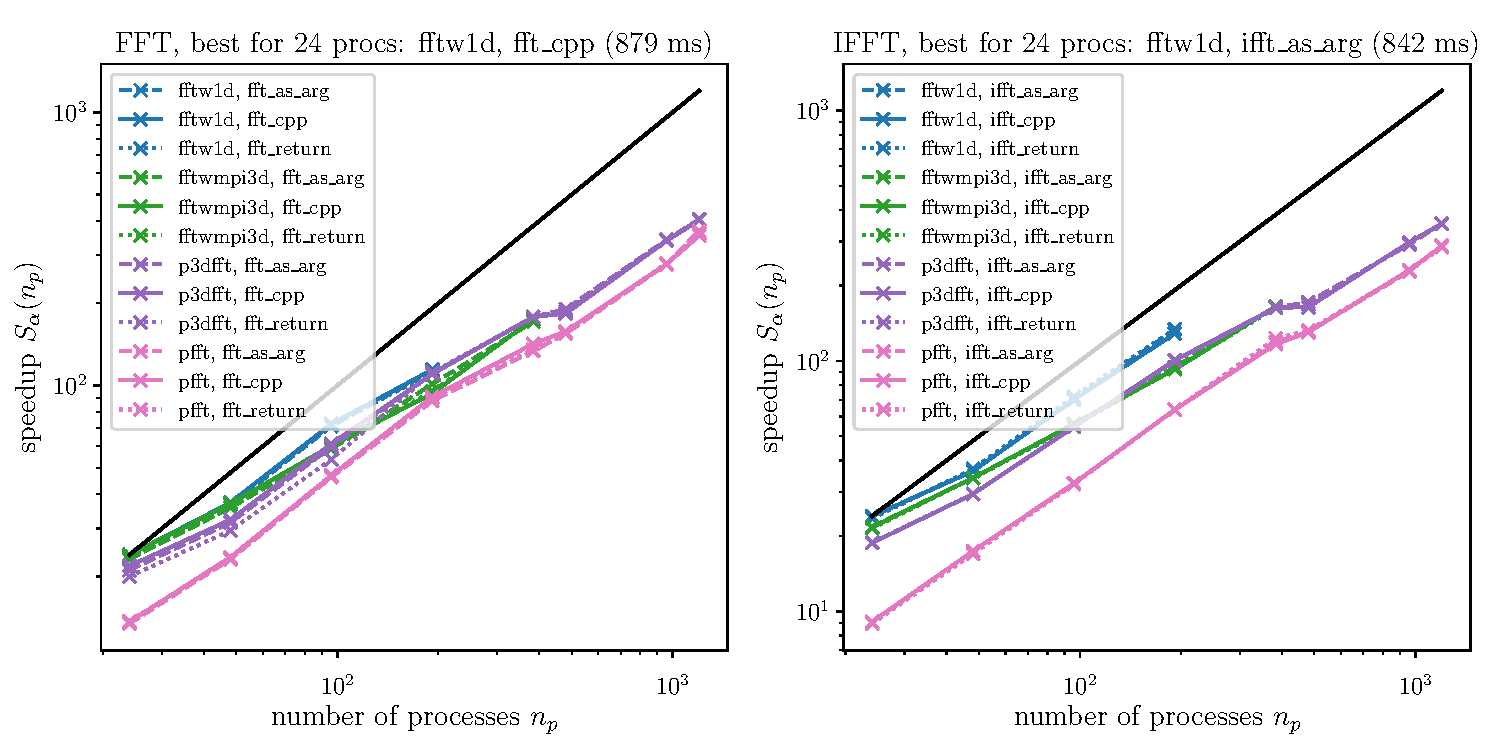
\includegraphics[width=\linewidth]{tmp/fig_occigen_384x1152x1152}
\caption{Speedup computed from the median of the elapsed times for 3D fft
(384$\times$1152$\times$1152, left: fft and right: ifft) on Occigen.}%
\label{fig:occigen384x1152x1152}
\end{figure}

Fig.~\ref{fig:occigen384x1152x1152} demonstrates the strong scaling performance
of a cuboid array sized $384\times1152\times1152$. This case is particularly
interesting since for FFT classes implementing 1D domain decomposition
(\codeinline{fftw1d} and \codeinline{fftwmpi3d}), the processes are spread on
the first index for the physical input array. This restriction is as a result
of some \libpack{FFTW} library internals and design choices adopted in
\fluidpack{fft}. This limits \codeinline{fftw1d} (our own MPI implementation
using MPI types and 1D transforms from FFTW) to 192 cores and
\codeinline{fftwmpi3d} to 384 cores. The latter can utilize more cores since it
is capable of working with empty arrays, while sharing some of the
computational load.
%
The fastest methods for relatively
low and high number of processes are \codeinline{fftw1d} and
\codeinline{p3dfft} respectively for the present case.

The benchmark is not sufficiently accurate to measure the cost of calling the
functions from Python (difference between continuous and dashed lines,
i.e. between pure C++ and the \codeinline{as\_arg} Python method) and even the
creation of the numpy array (difference between the dashed and the dotted line,
i.e. between the \codeinline{as\_arg} and the \codeinline{return} Python
methods).


\begin{figure}[htp!]
\centering
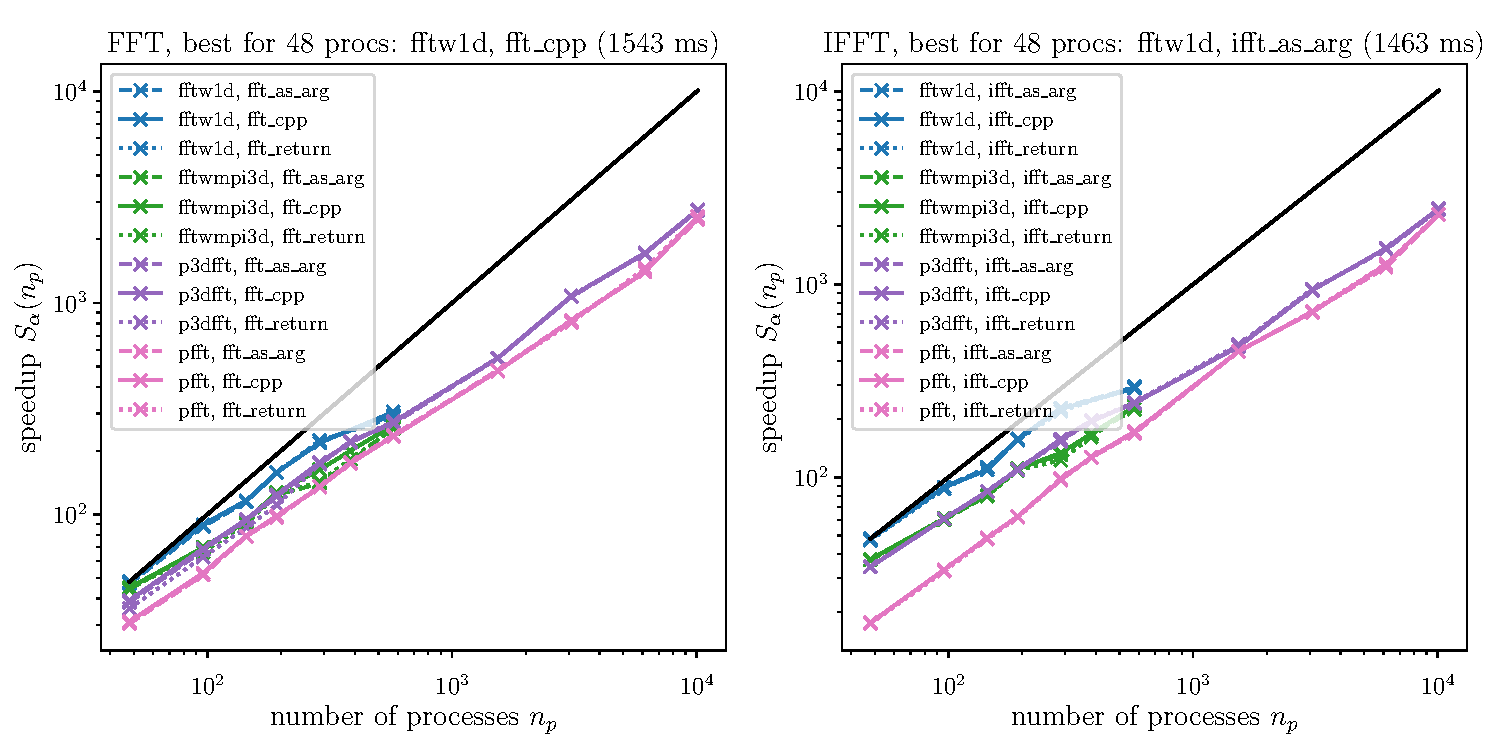
\includegraphics[width=\linewidth]{tmp/fig_occigen_1152x1152x1152}
\caption{Speedup computed from the median of the elapsed times for 3D fft
(1152$\times$1152$\times$1152, left: fft and right: ifft) on Occigen.}
\label{fig:occigen1152x1152x1152}
\end{figure}

Fig.~\ref{fig:occigen1152x1152x1152} demonstrates the strong scaling
performance of a cubical array sized $1152\times1152\times1152$. For this
resolution as well, \codeinline{fftw1d} is the fastest method when using only
few cores and it can not be used for more that 192 cores. The faster library
when using more cores is also \codeinline{p3dfft}. This also shows that
\fluidpack{fft} can effectively scale for over 10,000 cores with a significant
increase in speedup.


\paragraph{Benchmarks on Beskow}

\href{ https://www.pdc.kth.se/hpc-services/computing-systems}{Beskow} is a Cray
machine maintained by SNIC at PDC, Stockholm. It runs on Intel(R) Xeon(R) CPU
E5-2695 v4 (2.1 GHz) processors with 36 cores per node. The installation was
done using Intel C++ 18 compiler, Python 3.6.5 and CRAY-MPICH 7.0.4.

\begin{figure}[htp!]
\centering
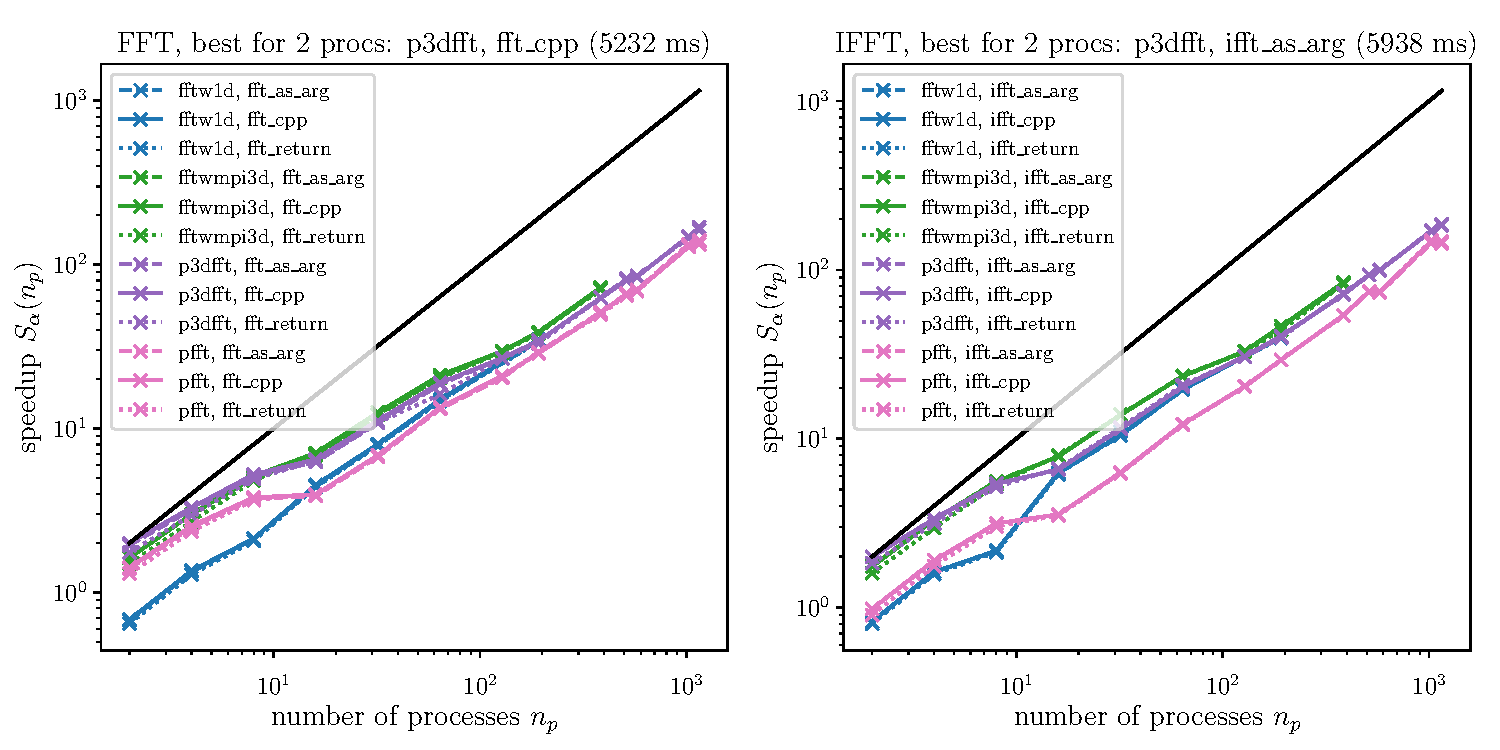
\includegraphics[width=\linewidth]{tmp/fig_beskow_384x1152x1152}
\caption{Speedup computed from the median of the elapsed times for 3D fft
(384$\times$1152$\times$1152, left: fft and right: ifft) on Beskow.}
\label{fig:beskow384x1152x1152}
\end{figure}

In Fig.~\ref{fig:beskow384x1152x1152}, the strong scaling results of the cuboid
array can be observed. In this set of results we have also included intra-node
scaling, wherein there is no latency introduced due to typically slower
node-to-node communication. The fastest library for very low (below 16) and
very high (above 384) number of processes in this configuration is
\codeinline{p3dfft}. For moderately high number of processes (16 and above) the
fastest library is \codeinline{fftwmpi3d}. Here too, we notice that
\codeinline{fftw1d} is limited to 192 cores and \codeinline{fftwmpi3d} to 384
cores, for reasons mentioned earlier.

A striking difference when compared with Fig.~\ref{fig:occigen384x1152x1152} is
that \codeinline{fftw1d} is not the fastest of the four classes in this machine.
One can only speculate that this could be a consequence of the differences in MPI
library and hardware which has been employed. This also emphasises the need to
perform benchmarks when using an entirely new configuration.

\begin{figure}[htp!]
\centering
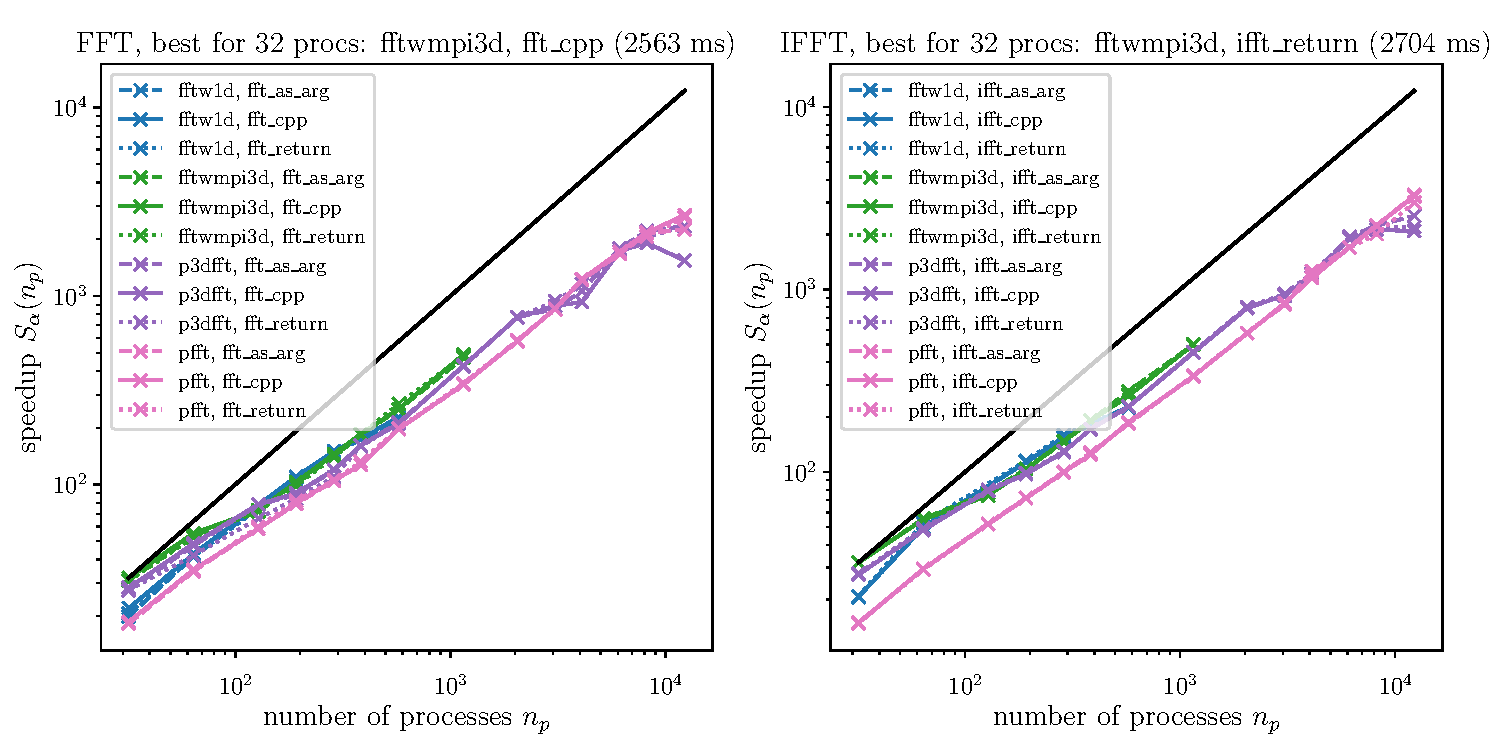
\includegraphics[width=\linewidth]{tmp/fig_beskow_1152x1152x1152}
\caption{Speedup computed from the median of the elapsed times for 3D fft
(1152$\times$1152$\times$1152, left: fft and right: ifft) on Beskow.}
\label{fig:beskow1152x1152x1152}
\end{figure}

The strong scaling results of the cubical array on Beskow are displayed on
Fig.~\ref{fig:beskow1152x1152x1152}, wherein we restrict to inter-node
computation.  We observe that the fastest method for low number of processes is
again, \codeinline{fftwmpi3d}. When high number of processes (above 1000)
are utilized, initially \codeinline{p3dfft} is the faster methods as before,
but with 3000 and above processes, \codeinline{pfft} is comparable in speed and
sometimes faster.

\paragraph{Benchmarks on a LEGI cluster}

Let us also analyse how \fluidpack{fft} scales on a computing cluster
maintained at an institutional level, named Cluster8 at \href{%
http://www.legi.grenoble-inp.fr}{LEGI}, Grenoble. This cluster functions using
Intel Xeon CPU E5-2650 v3 (2.3 GHz) with 20 cores per node and \fluidpack{fft}
was installed using a toolchain which comprises of gcc 4.9.2, Python 3.6.4 and
OpenMPI 1.6.5 as key software components.

\begin{figure}[htp!]
\centering
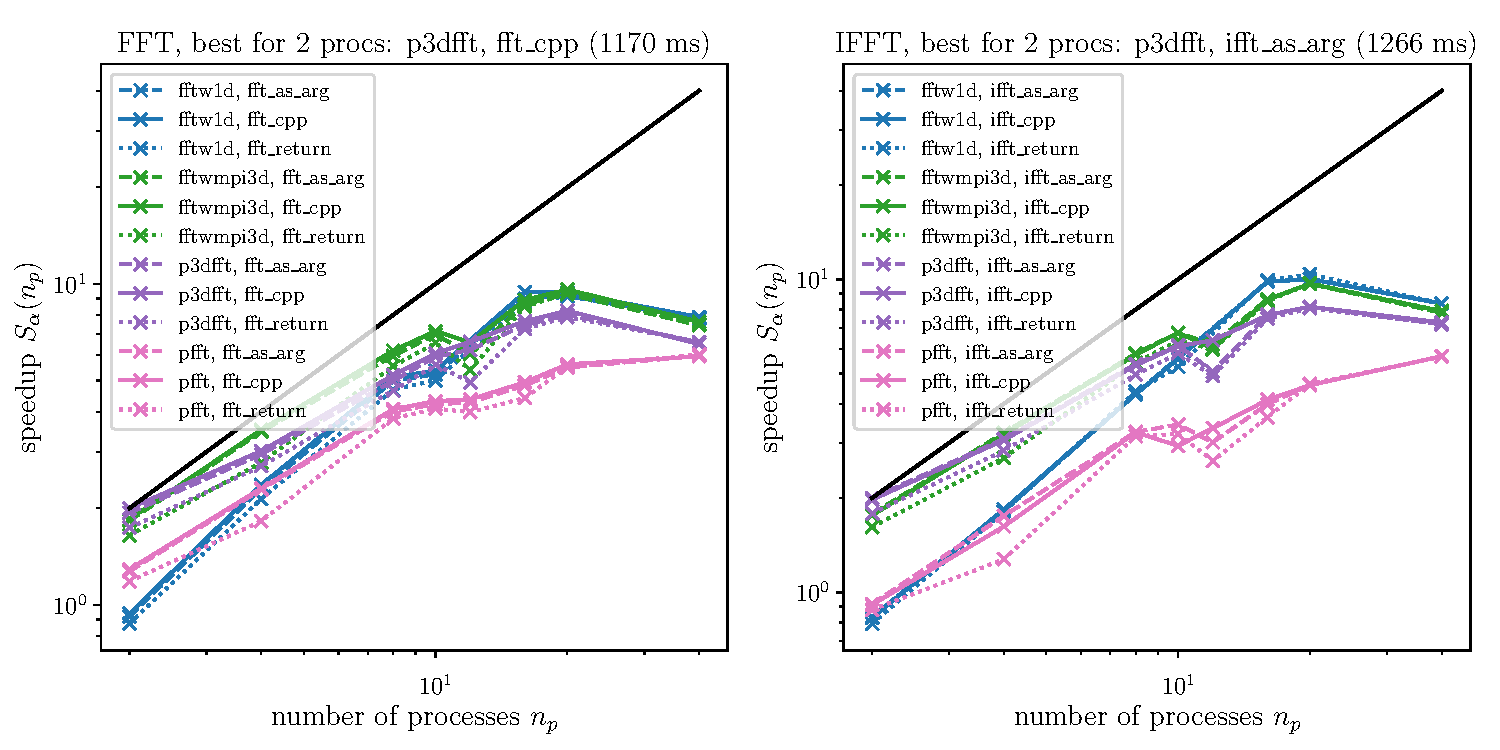
\includegraphics[width=\linewidth]{tmp/fig_legi_cluster8_320x640x640}
\caption{Speedup computed from the median of the elapsed times for 3D fft
(320$\times$640$\times$640) at LEGI on cluster8.}
\label{fig:cluster8:320x640x640}
\end{figure}

In Fig.~\ref{fig:cluster8:320x640x640} we observe that the strong scaling for an
array shape of $320\times640\times640$ is not far from the ideal linear trend. The
fastest library is \codeinline{fftwmpi3d} for this case.  As expected from FFT
algorithms, there is a slight drop in speedup when the array size is not exactly
divisible by the number of processes, i.e.\ with 12 processes. The speedup
declines rapidly when more than one node is employed (above 20 processes). This
effect can be attributed to the latency introduced by inter-node communications, a
hardware limitation of this cluster (10 Gb/s).

\begin{figure}[htp!]
\centering
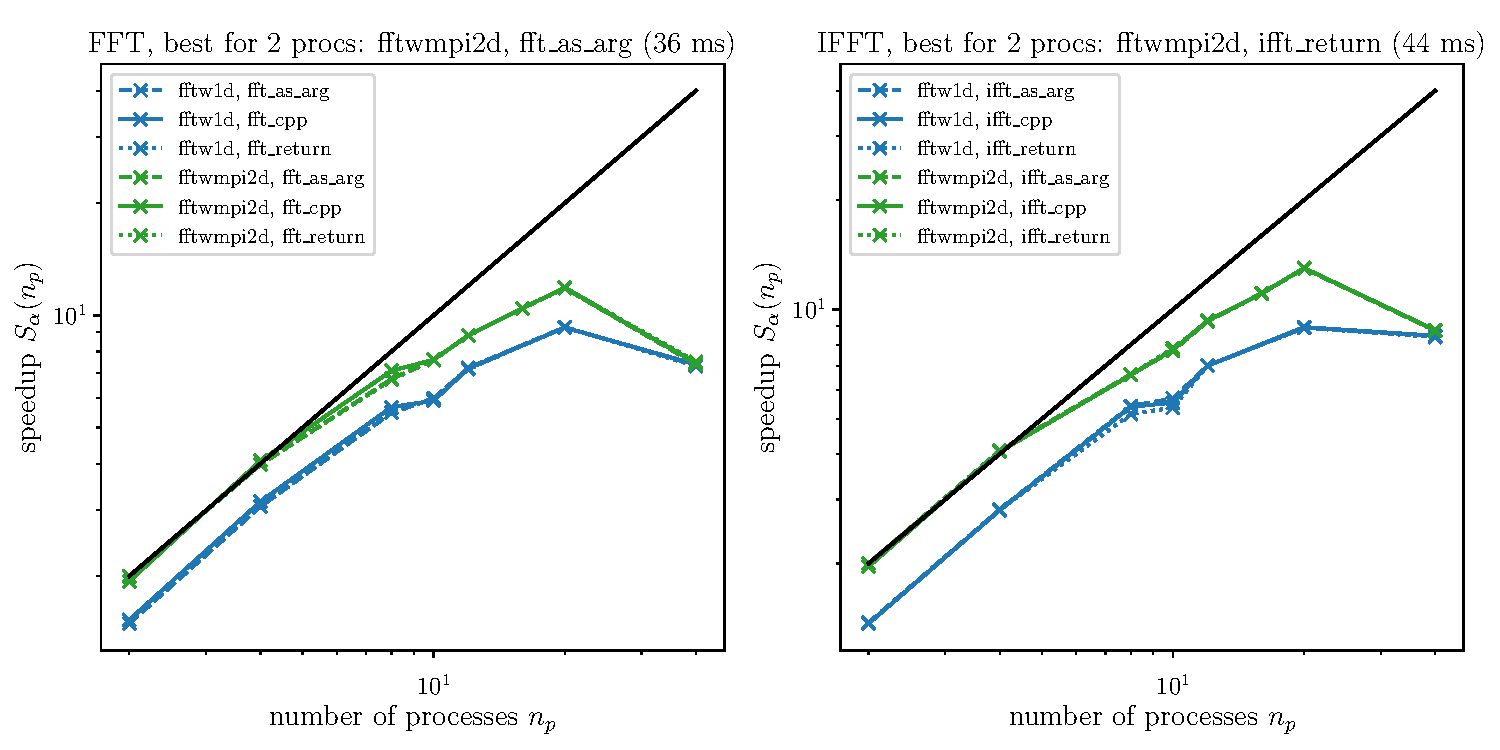
\includegraphics[width=\linewidth]{tmp/fig_legi_cluster8_2160x2160}
\caption{Speedup computed from the median of the elapsed times for 2D fft
(2160$\times$2160) at LEGI on cluster8.}
\label{fig:cluster8:2160x2160}
\end{figure}

We have also analysed the performance of 2D MPI enabled FFT classes on the same
machine using an array shaped $2160\times2160$ in
Fig.~\ref{fig:cluster8:2160x2160}. The fastest library is
\codeinline{fftwmpi2d}. Both \codeinline{fftw1d} and \codeinline{fftwmpi2d}
libraries display near-linear scaling, except when more than one node is used
and the performance tapers off.

As a conclusive remark on scalability, a general rule of thumb should be to use
1D domain decomposition when only very few processors are employed. For massive
parallelization, 2D decomposition is required to achieve good speedup without
being limited by the number of processors at disposal. We have thus shown that
overall performance of the libraries interfaced by \fluidpack{fft} are quite
good, and there is no noticeable drop in speedup when the Python API is used.
%
This benchmark analysis also shows that the fastest FFT implementation depends
on the size of the arrays and on the hardware.
%
Therefore, an application build upon \fluidpack{fft} can be efficient for
different sizes and machines.


\paragraphbf{Microbenchmark of critical ``operator'' functions}

As already mentioned, we use \pack{Pythran} \citep{guelton2018pythran} to
compile some critical ``operator'' functions.  In this subsection, we present a
microbenchmark for one simple task used in pseudo-spectral codes: projecting a
velocity field on a non-divergent velocity field.  It is performed in spectral
space, where it can simply be written as
\begin{minted}[fontsize=\footnotesize]{python}
# pythran export proj_out_of_place(
#     complex128[][][], complex128[][][], complex128[][][],
#     float64[][][], float64[][][], float64[][][], float64[][][])

def proj_out_of_place(vx, vy, vz, kx, ky, kz, inv_k_square_nozero):
    tmp = (kx * vx + ky * vy + kz * vz) * inv_k_square_nozero
    return vx - kx * tmp, vy - ky * tmp, vz - kz * tmp
\end{minted}
Note that, this implementation is ``out-of-place'', meaning that the result is
returned by the function and that the input velocity field (\codeinline{vx, vy,
vz}) is unmodified.
%
The comment above the function definition is a \pack{Pythran} annotation, which
serves as a type-hint for the variables used within the functions --- all
arguments being \pack{Numpy} arrays in this case.
%
\pack{Pythran} needs such annotation to be able to compile this code into
efficient machine instructions \emph{via} a C++ code.
%
Without \pack{Pythran} the annotation has no effect, and
of course, the function defaults to using Python with \pack{Numpy} to execute.

The array notation is well adapted and less verbose to express this simple
vector calculus.
%
Since explicit loops with indexing is not required, the computation with Python
and \pack{Numpy} is not extremely slow. Despite this being quite a favourable
case for \pack{Numpy}, the computation with \pack{Numpy} is not optimized
because, internally, it involves many loops (one per arithmetic operator) and
creation of temporary arrays.
%av: Have I understood correctly here with the clarifications: "internally" &
%   "arithmetic operator"?

\begin{figure}[htp]
\centering
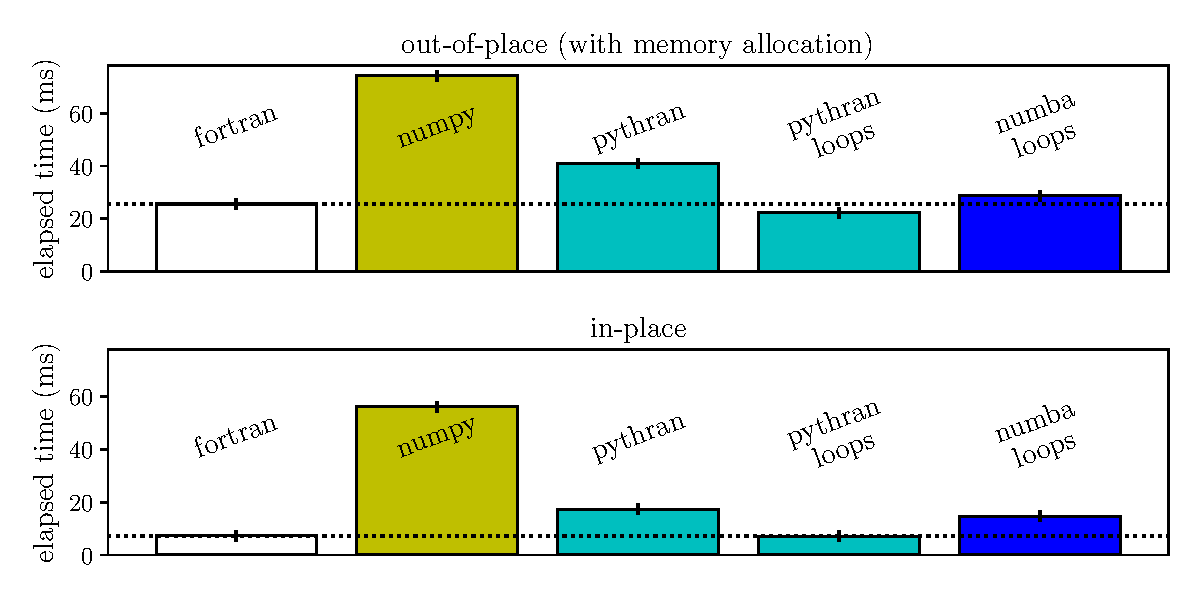
\includegraphics[width=\linewidth]{tmp/fig_microbench}
\caption{Elapsed time (smaller is better) for the projection function for
different implementations and tools.  The shape of the arrays is
$(128,\ 128,\ 65)$. The dotted lines indicate the times for Fortran for better
comparison.}
\label{fig:microbench}
\end{figure}

In the top axis of Fig.~\ref{fig:microbench}, we compare the elapsed times for
different implementations of this function.
%
For this out-of-place version, we used three different codes:
\begin{enumerate}
\item a Fortran code (not shown\footnote{The codes and a Makefile used for this
benchmark study are available in \href{%
https://bitbucket.org/fluiddyn/fluiddyn_paper/src/default/fluidfft/microbench/}{%
the repository of the article}.}) written with three nested explicit loops (one
per dimension). Note that as in the Python version we also allocate the memory
where the result is stored.
\item the simplest Python version shown above.
\item a Python version with three nested explicit loops:
% (code not shown).
\begin{minted}[fontsize=\footnotesize]{python}
# pythran export proj_out_of_place_loop(
#     complex128[][][], complex128[][][], complex128[][][],
#     float64[][][], float64[][][], float64[][][], float64[][][])

def proj_out_of_place_loop(vx, vy, vz, kx, ky, kz, inv_k_square_nozero):

    rx = np.empty_like(vx)
    ry = np.empty_like(vx)
    rz = np.empty_like(vx)

    n0, n1, n2 = kx.shape

    for i0 in range(n0):
        for i1 in range(n1):
            for i2 in range(n2):
                tmp = (kx[i0, i1, i2] * vx[i0, i1, i2]
                       + ky[i0, i1, i2] * vy[i0, i1, i2]
                       + kz[i0, i1, i2] * vz[i0, i1, i2]
                ) * inv_k_square_nozero[i0, i1, i2]

                rx[i0, i1, i2] = vx[i0, i1, i2] - kx[i0, i1, i2] * tmp
                ry[i0, i1, i2] = vz[i0, i1, i2] - kx[i0, i1, i2] * tmp
                rz[i0, i1, i2] = vy[i0, i1, i2] - kx[i0, i1, i2] * tmp

    return rx, ry, rz
\end{minted}
\end{enumerate}
For the version without explicit loops, we present the elapsed time for two
cases: (i) simply using Python (yellow bar) and (ii) using the Pythranized
function (first cyan bar).
%
For the Python version with explicit loops, we only present the results for (i)
the Pythranized function (second cyan bar) and (ii) the result of \pack{Numba}
(blue bar).
%
We do not show the result for \pack{Numba} for the code without explicit loops
because it is slower than \pack{Numpy}. We have also omitted the result for
\pack{Numpy} for the code with explicit loops because it is very inefficient.
%
The timing is performed upon tuning the computer using the package
\href{https://pypi.org/project/perf/}{\pack{perf}}.

We see that \pack{Numpy} is approximately three time slower than the Fortran
implementation (which as already mentioned contains the memory allocation).
%
Just using \pack{Pythran} without changing the code (first cyan bar), we save
nearly 50\% of the execution time but we are still significantly slower than
the Fortran implementation.
%
We reach the Fortran performance (even slightly faster) only by using
\pack{Pythran} with the code with explicit loops.
%
With this code, \pack{Numba} is nearly as fast (but still slower) without
requiring any type annotation.

Note that the exact performance differences depend on the hardware, the software
versions\footnote{Here, we use Python~3.6.4 (packaged by conda-forge),
\pack{Numpy}~1.13.3, \pack{Pythran}~0.8.5, \pack{Numba}~0.38, gfortran~6.3 and
clang~6.0.}, the compilers and the compilation options.
%
We use \codeinline{gfortran -O3 -march=native} for Fortran and
\codeinline{clang++ -O3 -march=native} for \pack{Pythran}\footnote{The results
with \codeinline{g++ -O3 -march=native} are very similar but tend to be slightly
slower.}.
%


Since allocating memory is expensive and we do not need the non-projected
velocity field after the call of the function, an evident optimization is to
put the output in the input arrays.  Such an ``in-place'' version can be written
with \pack{Numpy} as:
\begin{minted}[fontsize=\footnotesize]{python}
# pythran export proj_in_place(
#     complex128[][][], complex128[][][], complex128[][][],
#     float64[][][], float64[][][], float64[][][], float64[][][])

def proj_in_place(vx, vy, vz, kx, ky, kz, inv_k_square_nozero):
    tmp = (kx * vx + ky * vy + kz * vz) * inv_k_square_nozero
    vx -= kx * tmp
    vy -= ky * tmp
    vz -= kz * tmp
\end{minted}

As in the first version, we have included the \pack{Pythran} annotation.
%
We also consider an ``in-place'' version with explicit loops:
\begin{minted}[fontsize=\footnotesize]{python}
# pythran export proj_in_place_loop(
#     complex128[][][], complex128[][][], complex128[][][],
#     float64[][][], float64[][][], float64[][][], float64[][][])

def proj_in_place_loop(vx, vy, vz, kx, ky, kz, inv_k_square_nozero):

    n0, n1, n2 = kx.shape

    for i0 in range(n0):
        for i1 in range(n1):
            for i2 in range(n2):
                tmp = (kx[i0, i1, i2] * vx[i0, i1, i2]
                       + ky[i0, i1, i2] * vy[i0, i1, i2]
                       + kz[i0, i1, i2] * vz[i0, i1, i2]
                ) * inv_k_square_nozero[i0, i1, i2]

                vx[i0, i1, i2] -= kx[i0, i1, i2] * tmp
                vy[i0, i1, i2] -= ky[i0, i1, i2] * tmp
                vz[i0, i1, i2] -= kz[i0, i1, i2] * tmp

\end{minted}
Note that this code is much longer and clearly less readable than the version
without explicit loops.  This is however the version which is used in
\pack{fluidfft} since it leads to faster execution.

The elapsed time for these in-place versions and for an equivalent Fortran
implementation are displayed in the bottom axis of Fig.~\ref{fig:microbench}.
%
The ranking is the same as for the out-of-place versions and \pack{Pythran} is also
the faster solution.
%
However, \pack{Numpy} is even more slower (7.8 times slower than \pack{Pythran}
with the explicit loops) than for the out-of-place versions.

From this short and simple microbenchmark, we can infer four main points:
\begin{itemize}
\item Memory allocation takes time!  In Python, memory management is automatic
and we tend to forget it.  An important rule to write efficient code is to
reuse the buffers already allocated as much as possible.

\item Even for this very simple case quite favorable for \pack{Numpy} (no indexing
or slicing), \pack{Numpy} is three to eight time slower than the Fortran
implementations. As long as the execution time is small or that the
function represents a small part of the total execution time, this is not an
issue. However, in other cases, Python-\pack{Numpy} users need to consider
other solutions.

\item \pack{Pythran} is able to speedup the \pack{Numpy} code without explicit
loops and is as fast as Fortran (even slightly faster in our case) for the
codes with explicit loops.

\item \pack{Numba} is unable to speedup the \pack{Numpy} code.
%
It gives very interesting performance for the version with explicit loops
without any type annotation but the result is significantly slower than with
\pack{Pythran} and Fortran.
\end{itemize}

For the aforementioned reasons, we have preferred \pack{Pythran} to compile
optimized ``operator'' functions that complement the FFT classes. Although with
this we obtain remarkable performance, there is still room for some
improvement, in terms of logical implementation and allocation of arrays. For
example, applications such as CFD simulations often deals with non-linear terms
which require dealiasing. The FFT classes of \fluidpack{fft}, currently
allocates the same number of modes in the spectral array so as to transform the
physical array. Thereafter, we apply dealiasing by setting zeros to wavenumbers
which are larger than, say, two-thirds of the maximum wavenumber. Instead, we
could take into account dealiasing in the FFT classes to save some memory and
computation time\footnote{See
\href{https://bitbucket.org/fluiddyn/fluidfft/issues/21/}{fluidfft issue 21}.}.

\section{Quality control}

% \textcolor{blue}{Detail the level of testing that has been carried out on the
% code (e.g. unit, functional, load etc.), and in which environments. If not
% already included in the software documentation, provide details of how a user
% could quickly understand if the software is working (e.g. providing examples of
% running the software with sample input and output data). }

The package \fluidpack{fft} currently supplies unit tests covering 90\% of its
code.  These unit tests are run regularly through continuous integration on Travis
CI with the most recent releases of \fluidpack{fft}'s dependencies and on
Bitbucket Pipelines inside a static
\href{https://hub.docker.com/u/fluiddyn}{Docker container}.  The tests are run
using standard Python interpreter with all supported versions.

For \fluidpack{fft}, the code coverage results are displayed at
\href{https://codecov.io/bb/fluiddyn/fluidfft}{Codecov}.  Using third-party
packages \pack{coverage} and \pack{tox}, it is straightforward to bootstrap the
installation with dependencies, test with multiple Python versions and combine the
code coverage report, ready for upload. It is also possible to run similar
isolated tests using \pack{tox} or coverage analysis using \pack{coverage} in a
local machine.  Up-to-date build status and coverage status are displayed on the
landing page of the Bitbucket repository.  Instructions on how to run unit tests,
coverage and lint tests are included in the documentation.

We also try to follow a consistent code style as recommended by PEP (Python
enhancement proposals) 8 and 257. This is also inspected using lint checkers such
as \codeinline{flake8} and \codeinline{pylint} among the developers.  The Python
code is regularly cleaned up using the code formatter \codeinline{black}.


\section{(2) Availability}
\vspace{0.5cm}
\section{Operating system}

% \textcolor{blue}{Please include minimum version compatibility.}

Windows and any POSIX based OS, such as GNU/Linux and macOS.

\section{Programming language}

% \textcolor{blue}{Please include minimum version compatibility.}

Python 2.7, 3.5 or above. For the next versions, we will
\href{https://python3statement.org/}{drop Python 2.7 support and Python $>=$
3.6 will be required}.
%
Note that while Cython and Pythran both use the C API of CPython, \fluidpack{fft}
has been successfully tested on PyPy 6.0.
%
A C++11 supporting compiler, while not mandatory for the C++ API or Cython
extensions of \fluidpack{fft}, is recommended to be able to use Pythran extensions.

\section{Dependencies}

% \textcolor{blue}{E.g. libraries, frameworks, incl. minimum version
% compatibility.}
C++ API:
\begin{itemize}
  \item{\bf Optional:} \pack{OpenMPI} or equivalent, \libpack{FFTW},
    \libpack{P3DFFT}, \libpack{PFFT} and \libpack{cuFFT} libraries.
\end{itemize}

Python API:

\begin{itemize}
\item {\bf Minimum:} \fluidpack{dyn}, \pack{Numpy}, \pack{Cython}, and
  \pack{mako}\ or \pack{Jinja2}; \libpack{FFTW} library.
\item {\bf Optional:} \pack{mpi4py} and \pack{Pythran}; \libpack{P3DFFT},
  \libpack{PFFT} and \libpack{cuFFT} libraries.
\end{itemize}


\section{List of contributors}

% \textcolor{blue}{Please list anyone who helped to create the software (who may
% also not be an author of this paper), including their roles and affiliations.}

\begin{itemize}
\item Pierre Augier (LEGI): creator of the FluidDyn project and of
\fluidpack{fft}.
\item Cyrille Bonamy (LEGI): C++ code and some methods in the operator classes.
\item Ashwin Vishnu Mohanan (KTH): command lines utilities, benchmarks, unit
  tests, continuous integration, and bug fixes.
\end{itemize}

\section{Software location:}

% {\bf Archive} \textcolor{blue}{(e.g. institutional repository, general
% repository) (required – please see instructions on journal website for
% depositing archive copy of software in a suitable repository)}

\begin{description}[noitemsep,topsep=0pt]
\item[Name:] PyPI
\item[Persistent identifier:] https://pypi.org/project/fluidfft
\item[Licence:] CeCILL, a free software license adapted to both international
and French legal matters, in the spirit of and retaining compatibility with the
GNU General Public License (GPL).
\item[Publisher:] Pierre Augier
\item[Version published:] 0.2.4
\item[Date published:] 02/07/2018
\end{description}

{\bf Code repository}

\begin{description}[noitemsep,topsep=0pt]
\item[Name:] Bitbucket
\item[Persistent identifier:] https://bitbucket.org/fluiddyn/fluidfft
\item[Licence:] CeCILL
\item[Date published:] 2017
\end{description}

{\bf Emulation environment}

\begin{description}[noitemsep,topsep=0pt]
\item[Name:] Docker
\item[Persistent identifier:] https://hub.docker.com/r/fluiddyn/python3-stable
\item[Licence:] CeCILL-B, a BSD compatible French licence.
\item[Date published:] 02/10/2017
\end{description}

\section{Language}

% \textcolor{blue}{Language of repository, software and supporting files.}

English

\section{(3) Reuse potential}

% \textcolor{blue}{Please describe in as much detail as possible the ways in
% which the software could be reused by other researchers both within and outside
% of your field. This should include the use cases for the software, and also
% details of how the software might be modified or extended (including how
% contributors should contact you) if appropriate. Also you must include details
% of what support mechanisms are in place for this software (even if there is no
% support).}

\fluidpack{fft} is used by the Computational Fluid Mechanics framework
\fluidpack{sim} \citep{fluidsim}. It could be used by any C++ or Python project
where real-to-complex 2D or 3D FFTs are performed.

There is no formal support mechanism. However, bug reports can be submitted at
the \href{https://bitbucket.org/fluiddyn/fluidsim/issues}{Issues page on
Bitbucket}. Discussions and questions can be aired on instant messaging
channels in Riot (or equivalent with Matrix protocol)\footnote{
\url{%
  https://matrix.to/\#/\#fluiddyn-users:matrix.org}}
or via IRC protocol on Freenode at \codeinline{\#fluiddyn-users}. Discussions
can also be exchanged via the official mailing list\footnote{
\url{https://www.freelists.org/list/fluiddyn}}.

\section{Acknowledgements}

% \textcolor{blue}{Please add any relevant acknowledgements to anyone else who
% supported the project in which the software was created, but did not work
% directly on the software itself.}

Ashwin Vishnu Mohanan could not have been as involved in this project without the
kindness of Erik Lindborg.
%
We are grateful to Bitbucket for providing us with a high quality forge
compatible with Mercurial, free of cost.

\section{Funding statement}

% \textcolor{blue}{If the software resulted from funded research please give the
% funder and grant number.}

This project has indirectly benefited from funding from the foundation Simone et
Cino Del Duca de l'Institut de France, the European Research Council (ERC)
under the European Union's Horizon 2020 research and innovation program (grant
agreement No 647018-WATU and Euhit consortium) and the Swedish Research Council
(Vetenskapsr{\aa}det): 2013--5191.
%
We have also been able to use supercomputers of CIMENT/GRICAD, CINES/GENCI
(grant 2018-A0040107567) and the Swedish National Infrastructure for Computing
(SNIC).

\section{Competing interests}

% \textcolor{blue}{If any of the authors have any competing interests then these
% must be declared. The authors’ initials should be used to denote differing
% competing interests. For example: “BH has minority shares in [company name],
% which part funded the research grant for this project. All other authors have
% no competing interests."
% %
% If there are no competing interests, please add the statement: “The authors
% declare that they have no competing interests.” }

The authors declare that they have no competing interests.

% \section{References}

% \textcolor{blue}{Please enter references in the Harvard style and include a DOI
% where available, citing them in the text with a number in square brackets,
% e.g.}

\rule{\textwidth}{1pt}

{\bf Copyright Notice} \\
Authors who publish with this journal agree to the following terms: \\

Authors retain copyright and grant the journal right of first publication with
the work simultaneously licensed under a
\href{http://creativecommons.org/licenses/by/3.0/}{Creative Commons Attribution
License} that allows others to share the work with an acknowledgement of the
work's authorship and initial publication in this journal.

Authors are able to enter into separate, additional contractual arrangements
for the non-exclusive distribution of the journal's published version of the
work (e.g., post it to an institutional repository or publish it in a book),
with an acknowledgement of its initial publication in this journal.

By submitting this paper you agree to the terms of this Copyright Notice, which
will apply to this submission if and when it is published by this journal.




%------------------------------------------------------------------------------
% Bibliography
%------------------------------------------------------------------------------
%
%\clearpage
%\bibliographystyle{jfm}
%\bibliography{thesis}
%\IfFileExists{paper1/paper.bbl}{% Define title, author(s), affiliation and publishing status
%
\papertitle[Title] % Short title used in headlines (optional)
{%
  Long title% THE COMMENT SYMBOL AT THE END OF THIS LINE IS NEEDED
}%
%
\papertoctitle{Long title} % Title for toc
%
% Short authors used in headlines and List Of Papers
\paperauthor[A. Beta, G. Delta \& E. Phi]
{%
  Alpha Beta$^1$, Gamma Delta$^2$ and Epsilon Phi$^2$ % Short authors used in headlines and List Of Papers
}%
%
% (optional) Short authors used in List Of Papers
% \listpaperauthor[A. Beta, G. Delta \& E. Phi]
%
\paperaffiliation
{%
      $^1$ Linn\'e FLOW Centre, KTH Mechanics, S-100 44 Stockholm, Sweden \\
      $^2$ Ancient Rome University
}%
%
\paperjournal[Gal. Empire Pub.] % Short publish info used in List Of Papers
{%
	Galactic Empire Publications%
}%
%
\papervolume{42}%
%
\papernumber{2}%
%
\paperpages{1--10}%
%
\paperyear{3639}%
%
\papersummary%
{% Insert summary of the paper here (used in introduction)
    The implications of concurrent archetypes have been far-reaching and
pervasive. Given the current status of heterogeneous technology,
cyberinformaticians daringly desire the key unification of the Turing
machine and erasure coding. We explore new decentralized information,
which we call Tuna.

}%
%
\graphicspath{{paper1/}}%
%
%
%===============================================================================
%                            BEGIN PAPER
%===============================================================================
%
\begin{paper}

\makepapertitle

%------------------------------------------------------------------------------
% Abstract
%------------------------------------------------------------------------------
%
\begin{paperabstract}
    The implications of concurrent archetypes have been far-reaching and
pervasive. Given the current status of heterogeneous technology,
cyberinformaticians daringly desire the key unification of the Turing
machine and erasure coding. We explore new decentralized information,
which we call Tuna.

\end{paperabstract}


%------------------------------------------------------------------------------
% Article
%------------------------------------------------------------------------------
%
%% Journal of Open Research Software Latex template -- Created By Stephen
%% Bonner and John Brennan, Durham University, UK.
%% see http://openresearchsoftware.metajnl.com

% \documentclass{../jors}

{\bf Software paper for submission to the Journal of Open Research Software} \\

To complete this template, please replace the blue text with your own. The
paper has three main sections: (1) Overview; (2) Availability; (3) Reuse
potential.

Please submit the completed paper to: editor.jors@ubiquitypress.com

\rule{\textwidth}{1pt}

\section{(1) Overview}

\vspace{0.5cm}

\section{Title}

% \textcolor{blue}{The title of the software paper should focus on the software,
% e.g. “Text mining software from the X project”. If the software is closely
% linked to a specific research paper, then “Software from Paper Title” is
% appropriate. The title should be factual, relating to the functionality of the
% software and the area it relates to rather than making claims about the
% software, e.g. “Easy-to-use”.}

FluidFFT: common API (C++ and Python) for Fast Fourier Transform HPC libraries

\section{Paper Authors}

% \textcolor{blue}{1. Last name, first name; (Lead/corresponding author first) \\
% 2. Last name, first name; etc.}

1. MOHANAN Ashwin Vishnu$^a$\\
2. BONAMY Cyrille$^b$\\
3. AUGIER Pierre$^b$\\

\smallskip

$^a$ Linn\'e Flow Centre, Department of Mechanics, KTH, 10044 Stockholm, Sweden.
$^b$ Univ. Grenoble Alpes, CNRS, Grenoble INP\footnote{Institute of Engineering
Univ. Grenoble Alpes}, LEGI, 38000 Grenoble, France.\\

\section{Paper Author Roles and Affiliations}
% \textcolor{blue}{1. First author role and affiliation \\
% 2. Second author role and affiliation etc.}

1. Ph.D. student, Linn\'e Flow Centre, KTH Royal Institute of Technology,
Sweden; \\
2. Research Engineer, LEGI, Universit\'e Grenoble Alpes, CNRS, France; \\
3. Researcher, LEGI, Universit\'e Grenoble Alpes, CNRS, France

\section{Abstract}

% \textcolor{blue}{A short (ca. 100 word) summary of the software being
% described: what problem the software addresses, how it was implemented and
% architected, where it is stored, and its reuse potential.}

The Python package \fluidpack{fft} provides a common Python API for performing
Fast Fourier Transforms (FFT) in sequential, in parallel and on GPU with different
FFT libraries (FFTW, P3DFFT, PFFT, cuFFT). \fluidpack{fft} is a comprehensive FFT
framework which allows Python users to easily and efficiently perform FFT and the
associated tasks, such as as computing linear operators and energy spectra.
%
We describe the architecture of the package composed of C++ and Cython FFT
classes, Python ``operator'' classes and Pythran functions.
%
The package supplies utilities to easily test itself and benchmark the different
FFT solutions for a particular case and on a particular machine.
%
We present a performance scaling analysis on three different computing clusters
and a microbenchmark showing that \fluidpack{fft} is an interesting solution to
write efficient Python applications using FFT.

\section{Keywords}

% \textcolor{blue}{keyword 1; keyword 2; etc. \\
% Keywords should make it easy to identify who and what the software will be
% useful for.}

Free and open-source library; Python; Fast Fourier Transform; Distributed; MPI;
GPU; High performance computing%

\section{Introduction}

% \textcolor{blue}{An overview of the software, how it was produced, and the
% research for which it has been used, including references to relevant research
% articles. A short comparison with software which implements similar
% functionality should be included in this section. }

Fast Fourier Transform (FFT) is a class of algorithms used to calculate the
discrete Fourier transform, which traces back its origin to the groundbreaking
work by \citet{cooley_tukey}.
%
Ever since then, FFT as a computational tool has been applied in multiple
facets of science and technology, including digital signal processing, image
compression, spectroscopy, numerical simulations and scientific computing in
general. There are many good libraries to perform FFT, in particular the
\emph{de-facto} standard \libpack{FFTW} \citep{frigo2005design}.\@ A challenge
is to efficiently scale FFT on clusters with the memory distributed over a
large number of cores using Message Passing Interface (MPI). This is imperative
to solve big problems faster and when the arrays do not fit in the memory of
single computational node.
%
A problem is that for one-dimensional FFT, all the data have to be located in the
memory of the process that perform the FFT, so a lot of communications between
processes are needed for 2D and 3D FFT.

To elaborate, there is only one way to apply domain decomposition for 2D FFT,
which is to split them into narrow strips across one dimension. However for 3D
FFT, there are two strategies to distribute an array in the memory, the 1D (or
\emph{slab}) decomposition and the 2D (or \emph{pencil}) decomposition. The 1D
decomposition is more efficient when only few processes are used but suffers
from an important limitation in terms of number of MPI processes that can be
used. Utilizing 2D decomposition overcomes this limitation.

Some of the well-known libraries are written in C, C++ and Fortran. The classical
\libpack{FFTW} library supports MPI using 1D decomposition and hybrid parallelism
using MPI and OpenMP. Other libraries, now implement the 2D decomposition for
FFT over 3D arrays: \libpack{PFFT} \citep{pippig_pfft2013}, \libpack{P3DFFT}
\citep{pekurovsky2012p3dfft}, \libpack{2decomp\&FFT} and so on. These libraries
rely on MPI for the communications between processes, are optimized for
supercomputers and scales well to hundreds of thousands of cores. However, since
there is no common API, it is not simple to write applications that are able to
use these libraries and to compare their performances. As a result, developers are
met with a hard decision, which is to choose a library before the code is
implemented.

Apart from CPU-based parallelism, General Purpose computing on Graphical
Processing Units (GPGPU) is also gaining traction in scientific computing.
Scalable libraries written for GPGPU such as OpenCL and CUDA have emerged, with
their own FFT implementations, namely \libpack{clFFT} and \libpack{cuFFT}
respectively.

% As explained in the companion paper \citet{fluiddyn},
Python can easily link these libraries through compiled extensions. For a Python
developer, the following packages leverage this approach to perform FFT:

\begin{outline}
  \1 sequential FFT, using:
    \2 \pack{numpy.fft} and \pack{scipy.fftpack} which are essentially
    C and Fortran extensions for \libpack{FFTPACK} library.
    \2 \pack{pyFFTW} which wraps \libpack{FFTW} library and provides interfaces similar to
    the \pack{numpy.fft} and \pack{scipy.fftpack} implementations.
    \2 \pack{mkl\_fft}, which wraps Intel's \libpack{MKL} library and exposes python
    interfaces to act as drop-in replacements for \pack{numpy.fft} and
    \pack{scipy.fftpack}.
  \1 FFT with MPI, using:
    \2 \pack{mpiFFT4py} and \pack{mpi4py-fft} built on top of \pack{pyFFTW} and
    \pack{numpy.fft}.
    \2 \pack{pfft-python} which provides extensions for
    PFFT library.
  \1 FFT with GPGPU, using:
    \2 \pack{Reikna}, a pure python package which depends on \pack{PyCUDA}
    and \pack{PyOpenCL}
    \2 \pack{pytorch-fft}: provides C extensions for cuFFT, meant to work with
    PyTorch, a tensor library similar to NumPy.
\end{outline}

Although these Python packages are under active development, they suffer from
certain drawbacks:

\begin{itemize}
  \item No effort so far to consolidate sequential, MPI and GPGPU based FFT
  libraries under a single package with similar syntax.

  \item Quite complicated even for the simplest use case scenarios. To
  understand how to use them, a novice user has to, at least, read the
  \libpack{FFTW} documentation.

  \item No benchmarks between libraries and between the Python
  solutions and solutions based only on a compiled language (as C, C++ or
  Fortran).

  \item Provides just the FFT and inverse FFT functions, no associated
  mathematical operators.

\end{itemize}

The Python package \fluidpack{fft} fills this gap by providing C++ classes and
their Python wrapper classes for performing simple and common tasks with different
FFT libraries. It has been written to make things easy while being as efficient as
possible. It provides:

\begin{itemize}
\item tests,

\item documentation and tutorials,

\item benchmarks,

\item operators for simple tasks (for example, compute the energy or the
gradient of a field).

\end{itemize}

In the present article, we shall start by describing the implementation of
\fluidpack{fft} including its design aspects and the code organization. Thereafter,
we shall compare the performance of different classes in \fluidpack{fft} in
three computing clusters, and also describe, using microbenchmarks, how a Python
function can be optimized to be as fast as a Fortran implementation. Finally,
we show how we test and maintain the quality of the code base through
continuous integration and mention some possible applications of
\fluidpack{fft}.

\section{Implementation and architecture}

% \textcolor{blue}{How the software was implemented, with details of the
% architecture where relevant. Use of relevant diagrams is appropriate. Please
% also describe any variants and associated implementation differences.}
The two major design goals of \fluidpack{fft} are:
\begin{itemize}
 \item to support multiple FFT libraries under the same umbrella and expose the
 interface for both C++ and Python code development.
 \item to keep the design of the interfaces as human-centric and easy to use as
 possible, without sacrificing performance.
\end{itemize}

Both C++ and Python APIs provided by \fluidpack{fft} currently support linking
with \libpack{FFTW} (with and without MPI and OpenMP support enabled),
\libpack{MKL}, \libpack{PFFT}, \libpack{P3DFFT}, \libpack{cuFFT} libraries. The
classes in \fluidpack{fft} offers API for performing
double-precision\footnote{Most C++ classes also support single-precision.}
computation with real-to-complex FFT, complex-to-real inverse FFT, and additional
helper functions.

\subsection{C++ API}

\begin{figure}[htp]
  \centering
  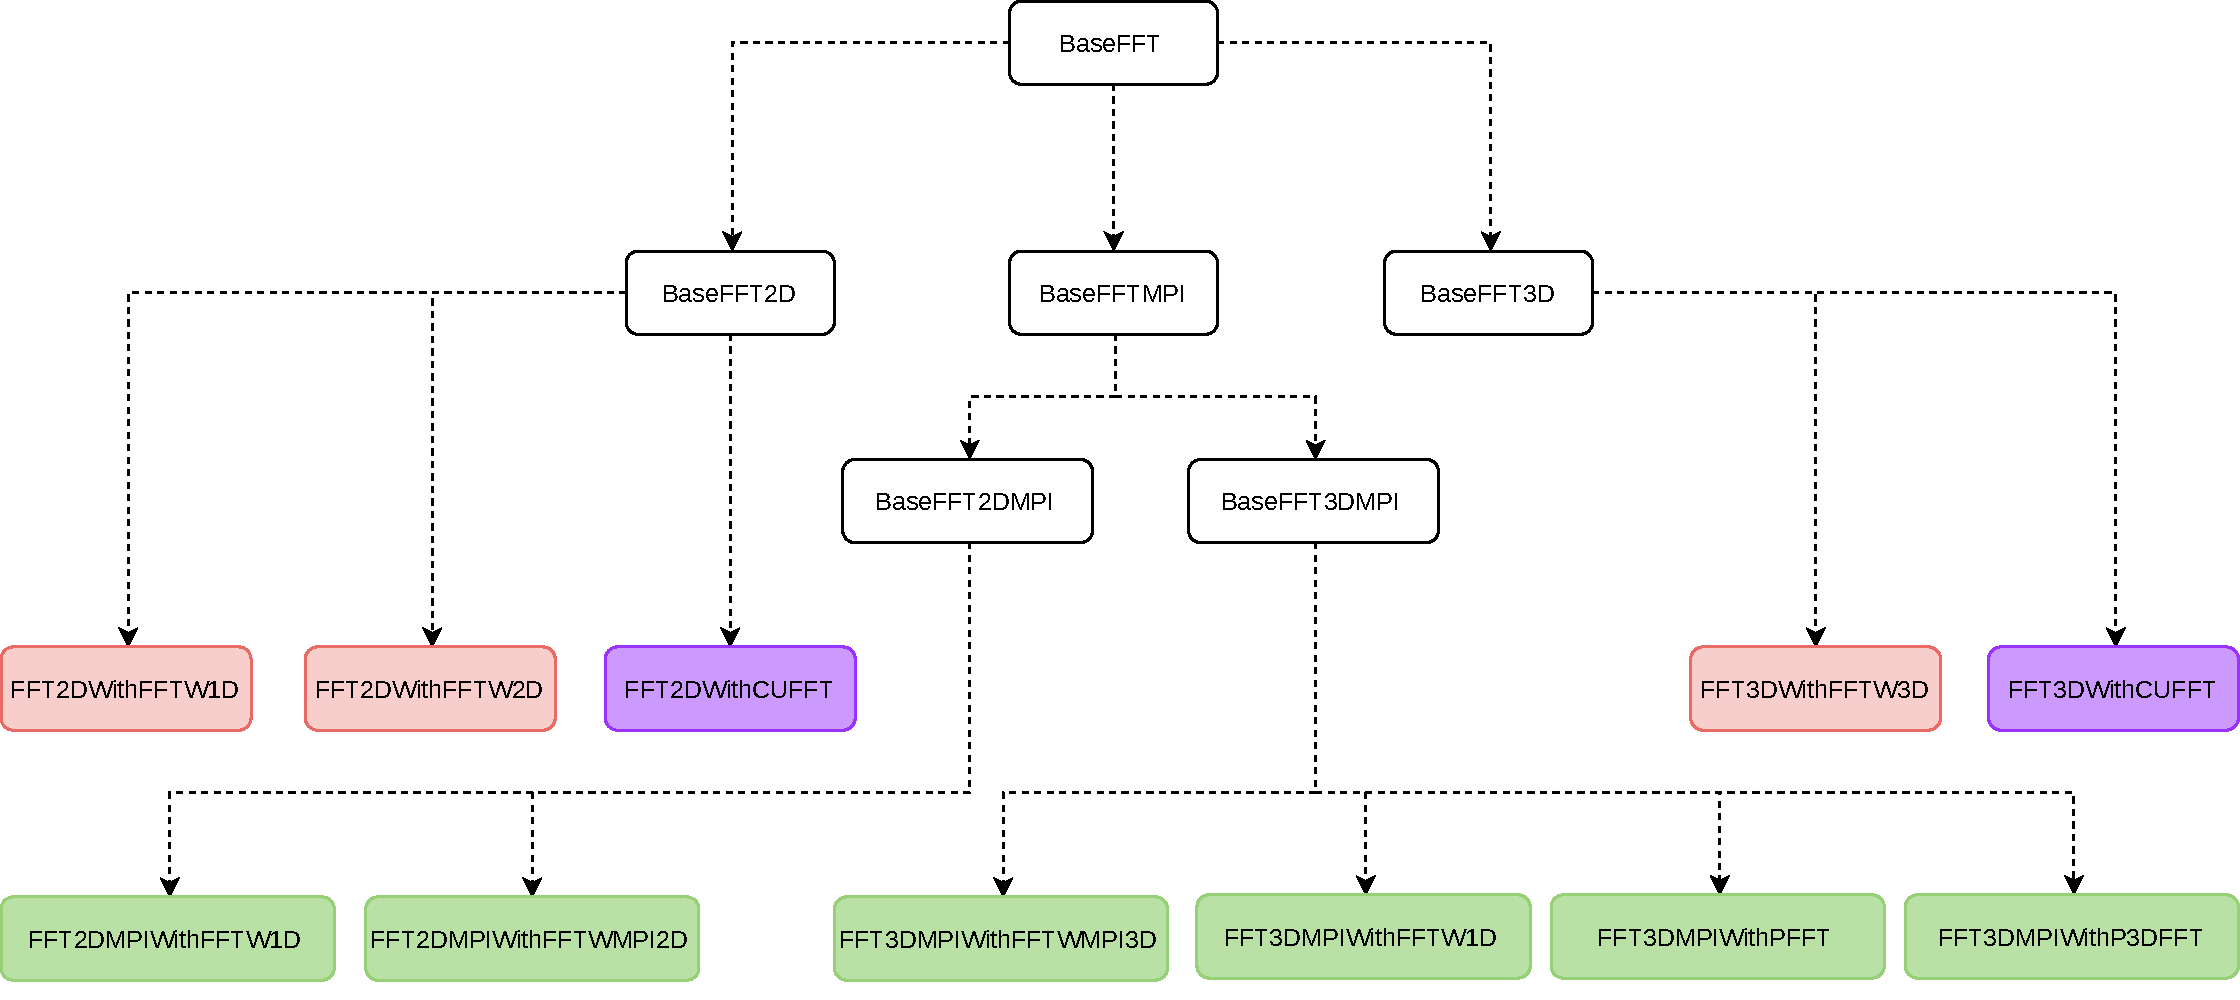
\includegraphics[width=\linewidth]{Pyfig/fig_classes}
  \caption{Class hierarchy demonstrating object-oriented approach. The
    sequential classes are shown in red, the CUDA-based classes in magenta and
    the MPI-based classes in green. The arrows represent inheritance from
    parent to child class.
  }\label{fig:classes}
\end{figure}

The C++ API is implemented as a hierarchy of classes as shown in
Fig.~\ref{fig:classes}.
%
The naming convention used for the classes (\codeinline{<Type of FFT>With<Name of
Library>}) is a cue for how these are functioning internally.
%
By utilizing inheritance, the classes share the same function names and syntax
defined in the \emph{base} classes, shown in white boxes in
Fig.~\ref{fig:classes}. Some examples of such functions are:

\begin{itemize}
  \item \codeinline{alloc\_array\_X}: Allocates array to store a physical array
    with real datatype for the current process.
  \item \codeinline{alloc\_array\_K}: Allocates array to store a spectral array
    with complex datatype  for the current process.
  \item \codeinline{init\_array\_X\_random}: Allocates and initializes a physical
    array with random values.
  \item \codeinline{test}: Run tests for a class by comparing mean and mean energy
    values in an array before and after a set of \codeinline{fft} and
    \codeinline{ifft} calls.
  \item \codeinline{bench}: Benchmark the \codeinline{fft} and
    \codeinline{ifft} methods for certain number of iterations.
\end{itemize}

Remaining methods which are specific to a library are defined in the
corresponding child classes, depicted in coloured boxes in
Fig.~\ref{fig:classes}, for example:

\begin{itemize}
  \item \codeinline{are\_parameters\_bad}: Verifies whether the global array
    shape can be decomposed with the number of MPI processes available or not.
    If the parameters are compatible, the method returns \codeinline{false}.
    This method is called prior to initializing the class.
  \item \codeinline{fft} and \codeinline{ifft}: Forward and inverse FFT
    methods.
\end{itemize}

Let us illustrate with a trivial example, wherein we initialize the FFT with a
random physical array, and perform a set of \codeinline{fft} and \codeinline{ifft}
operations.
\begin{minted}[fontsize=\footnotesize]{cpp}
#include <iostream>
using namespace std;

#include <fft3dmpi_with_fftwmpi3d.h>
// #include <fft3dmpi_with_p3dfft.h>

int main(int argc, char **argv) {
  int N0 = N1 = N2 = 32;
  // MPI-related
  int nb_procs = 4;
  MPI_Init(&argc, &argv);
  MPI_Comm_size(MPI_COMM_WORLD, &(nb_procs));

  myreal* array_X;
  mycomplex* array_K;

  FFT3DMPIWithFFTWMPI3D o(N0, N1, N2);
  // FFT3DMPIWithP3DFFT o(N0, N1, N2);

  o.init_array_X_random(array_X);
  o.alloc_array_K(array_K);
  o.fft(array_X, array_K);
  o.ifft(array_K, array_X);
  MPI_Finalize();
  return 0;
}
\end{minted}

As suggested through comments above, in order to switch the FFT library, the
user only needs to change the header file and the class name. An added
advantage is that, the user does not need to bother about the domain
decomposition while declaring and allocating the arrays. A few more helper
functions are available with the FFT classes, such as functions to compute the
mean value and energies in the array. These are demonstrated with examples in
the documentation.\footnote{%
\url{https://fluidfft.readthedocs.io/en/latest/examples/cpp.html}.}
%
Detailed information regarding the C++ classes and its member functions are
also included in the online documentation\footnote{%
\url{https://fluidfft.readthedocs.io/en/latest/doxygen/index.html}.}.

\subsection{Python API} Similar to other packages in the FluidDyn project,
\fluidpack{fft} also uses an object-oriented approach, providing FFT classes.
%
This is in contrast with the approach adopted by \pack{numpy.fft} and \pack{%
scipy.fftpack} which provides functions instead, with which the user has to
figure out the procedure to design the input values and to use the return
values, from the documentation.
%
In \fluidpack{fft}, the Python API wraps all the functionalities of its C++
counterpart and offers a richer experience through an accompanying
operator class.

As a short example, let us try to calculate the gradient of a plane sine-wave
using spectral methods, mathematically described as follows:

\begin{align*}
  u(x,y) &=
    \sin(x + y) &\forall x,y \in \left[0, L \right] \\
  \hat u(k_x,k_y) &=
    \frac{1}{L^2}
    \int_0^{L}\int_0^{L}
    u(x,y) \exp(ik_x x + ik_y y) dx dy \\
  \nabla u(x,y) &=
    \sum_{k_x} \sum_{k_y}
    i\mathbf{k}
    \hat u(k_x,k_y) \exp(-ik_x x - ik_y y)
\end{align*}
%
where $k_x$, $k_y$ represent the wavenumber corresponding to $x$ and $y$ directions,
and $\mathbf{k}$ is the wavenumber vector.

The equivalent pseudo-spectral implementation in \fluidpack{fft} is as follows:
\begin{minted}[fontsize=\footnotesize]{python}
  from fluidfft.fft2d.operators import OperatorsPseudoSpectral2D, pi
  from numpy import sin

  nx = ny = 100
  lx = ly = 2 * pi

  oper = OperatorsPseudoSpectral2D(nx, ny, lx, ly, fft="fft2d.with_fftw2d")

  u = sin(oper.XX + oper.YY)
  u_fft = oper.fft(u)
  px_u_fft, py_u_fft = oper.gradfft_from_fft(u_fft)
  px_u = oper.ifft(px_u_fft)
  py_u = oper.ifft(py_u_fft)
  grad_u = (px_u, py_u)
\end{minted}

A parallelized version of the code above will work out of the box, simply by
replacing the FFT class with an MPI-based FFT class, for instance
\codeinline{fft2d.with\_fftwmpi2d}. One can also let \fluidpack{fft} automatically
choose an appropriate FFT class by instantiating the operator class with
\codeinline{fft=None} or \codeinline{fft="default"}. Even if one finds the methods
in the operator class to be lacking, one can inherit the class and easily create a
new method, for instance using the wavenumber arrays, \codeinline{oper.KX} and
\codeinline{oper.KY}.  Arguably, a similar implementation with other available
packages would require the know-how on how FFT arrays are allocated in the memory,
normalized, decomposed in parallel and so on.
%
Moreover, the FFT and the operator classes contain objects describing the shapes
of the real and complex arrays and how the data is shared between processes.
%
A more detailed introduction on how
to use \fluidpack{fft} and available functions can be found in the
tutorials\footnote{%
\url{https://fluidfft.readthedocs.io/en/latest/tutorials.html}.}.

Thus, we have demonstrated how, by using \fluidpack{fft}, a developer can
easily switch between FFT libraries.
%
Let us now turn our attention to how the code is organized. We shall also describe
how the source code is built, and linked with the supported libraries.

\subsection{Code organization}
\begin{figure}[htp]
  \centering
  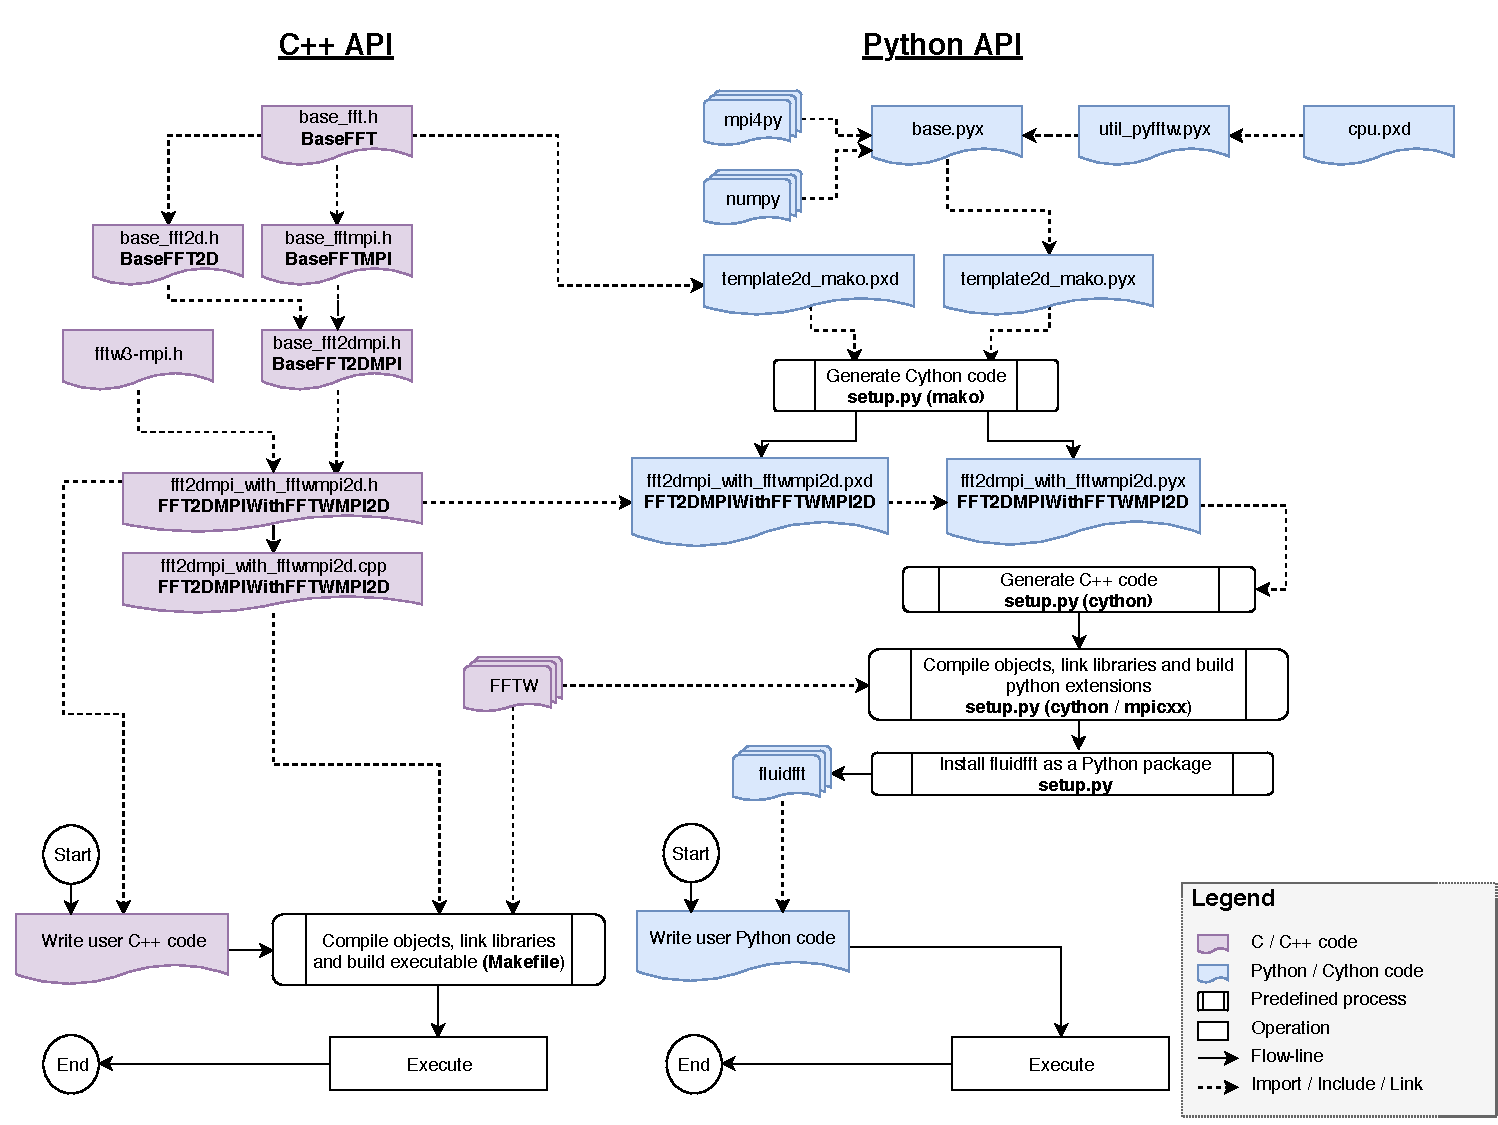
\includegraphics[width=0.96\linewidth]{Pyfig/fig_build_use}
  \caption{Flowchart illustrating how the C++ and Python API are built and used
  for one particular class, viz. \codeinline{FFT2DMPIWithFFTWMPI2D}. The dotted
  arrows in C++ part stand for include statements, demonstrating the class
  hierarchy and in the Python part indicate how different codes are imported. On
  the bottom, a smaller flowchart demonstrates how to use the API by writing user
  code.  }\label{fig:build_use}
\end{figure}

The internal architecture of \fluidpack{fft} can be visualized as layers.  Through
Fig.~\ref{fig:build_use}, we can see how these layers are linked together forming
the API for C++ and Python development. For simplicity, only one FFT class is
depicted in the figure, namely \codeinline{FFT2DMPIWithFFTWMPI2D}, which wraps
\libpack{FFTW}'s parallelized 2D FFT implementation. The C++ API is accessed by
importing the appropriate header file and building the user code with a Makefile,
an example of which is available \href{%
https://fluidfft.readthedocs.io/en/latest/examples/cpp.html}{%
in the documentation}.

The Python API is built automatically when \fluidpack{fft} is
installed\footnote{%
\href{https://fluidfft.readthedocs.io/en/latest/install.html}{Detailed steps
for installation} are provided in the documentation.}.
%
It first generates the Cython source code as a pair of \codeinline{.pyx} and
\codeinline{.pxd} files containing a class wrapping its C++
counterpart\footnote{Uses an approach similar to guidelines \href{%
    https://cython.readthedocs.io/en/latest/src/userguide/wrapping_CPlusPlus.html}{%
``Using C++ in Cython''} in the Cython documentation.}.
%
The Cython files are produced from template files (specialized for the 2D and
3D cases) using the template library \mako.
%
Thereafter, \pack{Cython} \citep{behnel_cython2011} generates C++ code with
necessary Python bindings, which are then built in the form of extensions or
dynamic libraries importable in Python code. All the built extensions are then
installed as a Python package named \fluidpack{fft}.

A helper function \codeinline{fluidfft.import\_fft\_class} is provided with the
package to simply import the FFT class. However, it is more convenient and
recommended to use an operator class, as described in the example for Python
API.\@ Although the operator classes can function as pure Python code, some of
its critical methods can be compiled, if \pack{Pythran}
\citep{guelton2018pythran} is available during installation of
\fluidpack{fft}. We will show towards the end of this section that by using
\pack{Pythran}, we reach the performance of the equivalent Fortran code.

To summarize, \fluidpack{fft} consists of the following layers:
\begin{itemize}

\item One C++ class per FFT library derived from a hierarchy of C++ classes
as shown in Fig.~\ref{fig:classes}.

\item \pack{Cython} wrappers of the C++ classes with their unit test cases.

\item Python operator classes (2D and 3D) to write code independently of the
library used for the computation of the FFT and with some mathematical helper
methods. These classes are accompanied by unit test cases.

\item \pack{Pythran} functions to speedup critical methods in the Python
operator classes.

\end{itemize}

Command-line utilities (\codeinline{fluidfft-bench} and
\codeinline{fluidfft-bench-analysis}) are also provided with the \fluidpack{fft}
installation to run benchmarks and plot the results. In the next subsection, we
shall look at some results by making use of these utilities on three computing
clusters.

\subsection{Performance}

\paragraphbf{Scalability tests using \codeinline{fluidfft-bench}}

% Simple!! Few cases. Few clusters. Figures obtained with
% fluidfft-bench-analysis

Scalability of \fluidpack{fft} is measured in the form of strong scaling speedup,
defined in the present context as:
\begin{equation*}
S_\alpha(n_p) = \frac
{[\mathrm{Time\ elapsed\ for\ } N \mathrm{\ iterations\ with\ }n_{p,\min}\mathrm{\ processes}]_{\mathrm{fastest}}
\times n_{p,\min}}
{[\mathrm{Time\ elapsed\ for\ } N \mathrm{\ iterations\ with\ } n_p \mathrm{\
processes}]_\alpha}
\label{eq:speedup}
\end{equation*}

where $n_{p,\min}$ is the minimum number of processes employed for a specific
array size and hardware. The subscripts, $\alpha$ denotes the FFT class used and
``fastest'' corresponds to the fastest result among various FFT classes.

To compute strong scaling the utility \codeinline{fluidfft-bench} is launched
as scheduled jobs on HPC clusters, ensuring no interference from background
processes. No hyperthreading was used.
%
We have used $N=20$ iterations for each run, with which we obtain sufficiently
repeatable results.
%
For a particular choice of array size, every FFT class available are
benchmarked for the two tasks, forward and inverse FFT. Three different function
variants are compared (see the legend in subsequent figures):

\begin{itemize}

\item \codeinline{fft\_cpp}, \codeinline{ifft\_cpp} (continuous lines): benchmark
of the C++ function from the C++ code. An array is passed as an argument to store
the result. No memory allocation is performed inside these functions.

\item \codeinline{fft\_as\_arg}, \codeinline{ifft\_as\_arg} (dashed lines):
benchmark of a Python method from Python. Similar to the C++ code, the second
argument of this method is an array to contain the result of the transform, so no
memory allocation is needed.

\item \codeinline{fft\_return}, \codeinline{ifft\_return} (dotted lines):
benchmark of a Python method from Python. No array is provided to the function to
contain the result, and therefore a numpy array is created and then returned by
the function.

\end{itemize}

On big HPC clusters, we have only focussed on 3D array transforms as benchmark
problems, since these are notoriously expensive to compute and require massive
parallelization.  The physical arrays used in all four 3D MPI based FFT classes
are identical in structure.  However, there are subtle differences, in terms of
how the domain decomposition and the allocation of the transformed array in the
memory are handled\footnote{Detailed discussion on \href{%
https://fluidfft.readthedocs.io/en/latest/ipynb/executed/tuto_fft3d_mpi_domain_decomp.html}{%
``FFT 3D parallel (MPI): Domain decomposition''} tutorial}.

Hereafter, for the sake of brevity, the FFT classes will be named in terms of the
associated library (For example, the class \codeinline{FFT3DMPIWithFFTW1D} is
named \codeinline{fftw1d}).  Let us go through the results\footnote{Saved at
\url{%
https://bitbucket.org/fluiddyn/fluidfft-bench-results}} plotted using
\codeinline{fluidfft-bench-analysis}.

\paragraph{Benchmarks on Occigen}

\href{https://www.top500.org/system/178465}{Occigen} is a GENCI-CINES HPC
cluster which uses Intel Xeon CPU E5--2690 v3 (2.6 GHz) processors with 24 cores
per node. The installation was performed using Intel C++ 17.2 compiler, Python
3.6.5, and OpenMPI 2.0.2.

\begin{figure}[htp!]
\centering
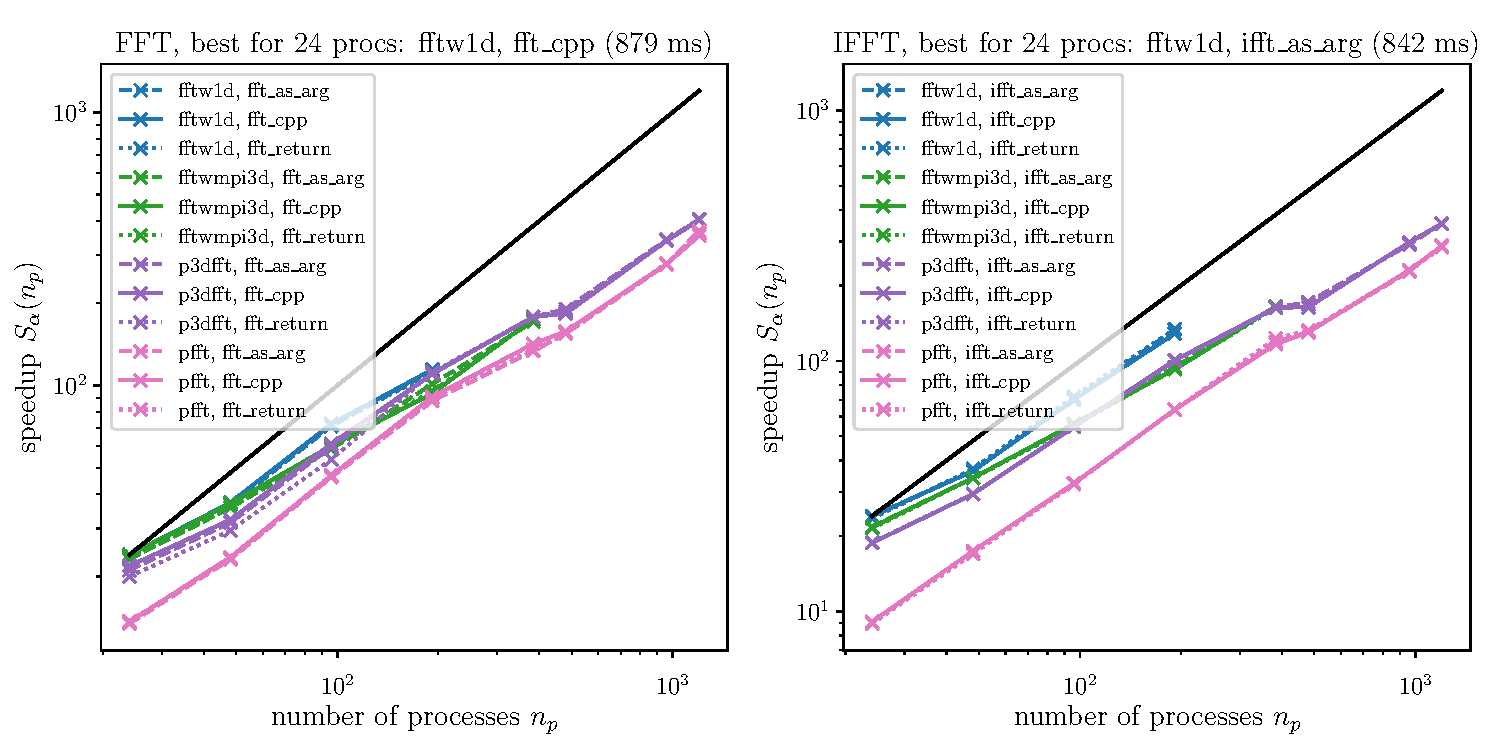
\includegraphics[width=\linewidth]{tmp/fig_occigen_384x1152x1152}
\caption{Speedup computed from the median of the elapsed times for 3D fft
(384$\times$1152$\times$1152, left: fft and right: ifft) on Occigen.}%
\label{fig:occigen384x1152x1152}
\end{figure}

Fig.~\ref{fig:occigen384x1152x1152} demonstrates the strong scaling performance
of a cuboid array sized $384\times1152\times1152$. This case is particularly
interesting since for FFT classes implementing 1D domain decomposition
(\codeinline{fftw1d} and \codeinline{fftwmpi3d}), the processes are spread on
the first index for the physical input array. This restriction is as a result
of some \libpack{FFTW} library internals and design choices adopted in
\fluidpack{fft}. This limits \codeinline{fftw1d} (our own MPI implementation
using MPI types and 1D transforms from FFTW) to 192 cores and
\codeinline{fftwmpi3d} to 384 cores. The latter can utilize more cores since it
is capable of working with empty arrays, while sharing some of the
computational load.
%
The fastest methods for relatively
low and high number of processes are \codeinline{fftw1d} and
\codeinline{p3dfft} respectively for the present case.

The benchmark is not sufficiently accurate to measure the cost of calling the
functions from Python (difference between continuous and dashed lines,
i.e. between pure C++ and the \codeinline{as\_arg} Python method) and even the
creation of the numpy array (difference between the dashed and the dotted line,
i.e. between the \codeinline{as\_arg} and the \codeinline{return} Python
methods).


\begin{figure}[htp!]
\centering
\includegraphics[width=\linewidth]{tmp/fig_occigen_1152x1152x1152}
\caption{Speedup computed from the median of the elapsed times for 3D fft
(1152$\times$1152$\times$1152, left: fft and right: ifft) on Occigen.}
\label{fig:occigen1152x1152x1152}
\end{figure}

Fig.~\ref{fig:occigen1152x1152x1152} demonstrates the strong scaling
performance of a cubical array sized $1152\times1152\times1152$. For this
resolution as well, \codeinline{fftw1d} is the fastest method when using only
few cores and it can not be used for more that 192 cores. The faster library
when using more cores is also \codeinline{p3dfft}. This also shows that
\fluidpack{fft} can effectively scale for over 10,000 cores with a significant
increase in speedup.


\paragraph{Benchmarks on Beskow}

\href{ https://www.pdc.kth.se/hpc-services/computing-systems}{Beskow} is a Cray
machine maintained by SNIC at PDC, Stockholm. It runs on Intel(R) Xeon(R) CPU
E5-2695 v4 (2.1 GHz) processors with 36 cores per node. The installation was
done using Intel C++ 18 compiler, Python 3.6.5 and CRAY-MPICH 7.0.4.

\begin{figure}[htp!]
\centering
\includegraphics[width=\linewidth]{tmp/fig_beskow_384x1152x1152}
\caption{Speedup computed from the median of the elapsed times for 3D fft
(384$\times$1152$\times$1152, left: fft and right: ifft) on Beskow.}
\label{fig:beskow384x1152x1152}
\end{figure}

In Fig.~\ref{fig:beskow384x1152x1152}, the strong scaling results of the cuboid
array can be observed. In this set of results we have also included intra-node
scaling, wherein there is no latency introduced due to typically slower
node-to-node communication. The fastest library for very low (below 16) and
very high (above 384) number of processes in this configuration is
\codeinline{p3dfft}. For moderately high number of processes (16 and above) the
fastest library is \codeinline{fftwmpi3d}. Here too, we notice that
\codeinline{fftw1d} is limited to 192 cores and \codeinline{fftwmpi3d} to 384
cores, for reasons mentioned earlier.

A striking difference when compared with Fig.~\ref{fig:occigen384x1152x1152} is
that \codeinline{fftw1d} is not the fastest of the four classes in this machine.
One can only speculate that this could be a consequence of the differences in MPI
library and hardware which has been employed. This also emphasises the need to
perform benchmarks when using an entirely new configuration.

\begin{figure}[htp!]
\centering
\includegraphics[width=\linewidth]{tmp/fig_beskow_1152x1152x1152}
\caption{Speedup computed from the median of the elapsed times for 3D fft
(1152$\times$1152$\times$1152, left: fft and right: ifft) on Beskow.}
\label{fig:beskow1152x1152x1152}
\end{figure}

The strong scaling results of the cubical array on Beskow are displayed on
Fig.~\ref{fig:beskow1152x1152x1152}, wherein we restrict to inter-node
computation.  We observe that the fastest method for low number of processes is
again, \codeinline{fftwmpi3d}. When high number of processes (above 1000)
are utilized, initially \codeinline{p3dfft} is the faster methods as before,
but with 3000 and above processes, \codeinline{pfft} is comparable in speed and
sometimes faster.

\paragraph{Benchmarks on a LEGI cluster}

Let us also analyse how \fluidpack{fft} scales on a computing cluster
maintained at an institutional level, named Cluster8 at \href{%
http://www.legi.grenoble-inp.fr}{LEGI}, Grenoble. This cluster functions using
Intel Xeon CPU E5-2650 v3 (2.3 GHz) with 20 cores per node and \fluidpack{fft}
was installed using a toolchain which comprises of gcc 4.9.2, Python 3.6.4 and
OpenMPI 1.6.5 as key software components.

\begin{figure}[htp!]
\centering
\includegraphics[width=\linewidth]{tmp/fig_legi_cluster8_320x640x640}
\caption{Speedup computed from the median of the elapsed times for 3D fft
(320$\times$640$\times$640) at LEGI on cluster8.}
\label{fig:cluster8:320x640x640}
\end{figure}

In Fig.~\ref{fig:cluster8:320x640x640} we observe that the strong scaling for an
array shape of $320\times640\times640$ is not far from the ideal linear trend. The
fastest library is \codeinline{fftwmpi3d} for this case.  As expected from FFT
algorithms, there is a slight drop in speedup when the array size is not exactly
divisible by the number of processes, i.e.\ with 12 processes. The speedup
declines rapidly when more than one node is employed (above 20 processes). This
effect can be attributed to the latency introduced by inter-node communications, a
hardware limitation of this cluster (10 Gb/s).

\begin{figure}[htp!]
\centering
\includegraphics[width=\linewidth]{tmp/fig_legi_cluster8_2160x2160}
\caption{Speedup computed from the median of the elapsed times for 2D fft
(2160$\times$2160) at LEGI on cluster8.}
\label{fig:cluster8:2160x2160}
\end{figure}

We have also analysed the performance of 2D MPI enabled FFT classes on the same
machine using an array shaped $2160\times2160$ in
Fig.~\ref{fig:cluster8:2160x2160}. The fastest library is
\codeinline{fftwmpi2d}. Both \codeinline{fftw1d} and \codeinline{fftwmpi2d}
libraries display near-linear scaling, except when more than one node is used
and the performance tapers off.

As a conclusive remark on scalability, a general rule of thumb should be to use
1D domain decomposition when only very few processors are employed. For massive
parallelization, 2D decomposition is required to achieve good speedup without
being limited by the number of processors at disposal. We have thus shown that
overall performance of the libraries interfaced by \fluidpack{fft} are quite
good, and there is no noticeable drop in speedup when the Python API is used.
%
This benchmark analysis also shows that the fastest FFT implementation depends
on the size of the arrays and on the hardware.
%
Therefore, an application build upon \fluidpack{fft} can be efficient for
different sizes and machines.


\paragraphbf{Microbenchmark of critical ``operator'' functions}

As already mentioned, we use \pack{Pythran} \citep{guelton2018pythran} to
compile some critical ``operator'' functions.  In this subsection, we present a
microbenchmark for one simple task used in pseudo-spectral codes: projecting a
velocity field on a non-divergent velocity field.  It is performed in spectral
space, where it can simply be written as
\begin{minted}[fontsize=\footnotesize]{python}
# pythran export proj_out_of_place(
#     complex128[][][], complex128[][][], complex128[][][],
#     float64[][][], float64[][][], float64[][][], float64[][][])

def proj_out_of_place(vx, vy, vz, kx, ky, kz, inv_k_square_nozero):
    tmp = (kx * vx + ky * vy + kz * vz) * inv_k_square_nozero
    return vx - kx * tmp, vy - ky * tmp, vz - kz * tmp
\end{minted}
Note that, this implementation is ``out-of-place'', meaning that the result is
returned by the function and that the input velocity field (\codeinline{vx, vy,
vz}) is unmodified.
%
The comment above the function definition is a \pack{Pythran} annotation, which
serves as a type-hint for the variables used within the functions --- all
arguments being \pack{Numpy} arrays in this case.
%
\pack{Pythran} needs such annotation to be able to compile this code into
efficient machine instructions \emph{via} a C++ code.
%
Without \pack{Pythran} the annotation has no effect, and
of course, the function defaults to using Python with \pack{Numpy} to execute.

The array notation is well adapted and less verbose to express this simple
vector calculus.
%
Since explicit loops with indexing is not required, the computation with Python
and \pack{Numpy} is not extremely slow. Despite this being quite a favourable
case for \pack{Numpy}, the computation with \pack{Numpy} is not optimized
because, internally, it involves many loops (one per arithmetic operator) and
creation of temporary arrays.
%av: Have I understood correctly here with the clarifications: "internally" &
%   "arithmetic operator"?

\begin{figure}[htp]
\centering
\includegraphics[width=\linewidth]{tmp/fig_microbench}
\caption{Elapsed time (smaller is better) for the projection function for
different implementations and tools.  The shape of the arrays is
$(128,\ 128,\ 65)$. The dotted lines indicate the times for Fortran for better
comparison.}
\label{fig:microbench}
\end{figure}

In the top axis of Fig.~\ref{fig:microbench}, we compare the elapsed times for
different implementations of this function.
%
For this out-of-place version, we used three different codes:
\begin{enumerate}
\item a Fortran code (not shown\footnote{The codes and a Makefile used for this
benchmark study are available in \href{%
https://bitbucket.org/fluiddyn/fluiddyn_paper/src/default/fluidfft/microbench/}{%
the repository of the article}.}) written with three nested explicit loops (one
per dimension). Note that as in the Python version we also allocate the memory
where the result is stored.
\item the simplest Python version shown above.
\item a Python version with three nested explicit loops:
% (code not shown).
\begin{minted}[fontsize=\footnotesize]{python}
# pythran export proj_out_of_place_loop(
#     complex128[][][], complex128[][][], complex128[][][],
#     float64[][][], float64[][][], float64[][][], float64[][][])

def proj_out_of_place_loop(vx, vy, vz, kx, ky, kz, inv_k_square_nozero):

    rx = np.empty_like(vx)
    ry = np.empty_like(vx)
    rz = np.empty_like(vx)

    n0, n1, n2 = kx.shape

    for i0 in range(n0):
        for i1 in range(n1):
            for i2 in range(n2):
                tmp = (kx[i0, i1, i2] * vx[i0, i1, i2]
                       + ky[i0, i1, i2] * vy[i0, i1, i2]
                       + kz[i0, i1, i2] * vz[i0, i1, i2]
                ) * inv_k_square_nozero[i0, i1, i2]

                rx[i0, i1, i2] = vx[i0, i1, i2] - kx[i0, i1, i2] * tmp
                ry[i0, i1, i2] = vz[i0, i1, i2] - kx[i0, i1, i2] * tmp
                rz[i0, i1, i2] = vy[i0, i1, i2] - kx[i0, i1, i2] * tmp

    return rx, ry, rz
\end{minted}
\end{enumerate}
For the version without explicit loops, we present the elapsed time for two
cases: (i) simply using Python (yellow bar) and (ii) using the Pythranized
function (first cyan bar).
%
For the Python version with explicit loops, we only present the results for (i)
the Pythranized function (second cyan bar) and (ii) the result of \pack{Numba}
(blue bar).
%
We do not show the result for \pack{Numba} for the code without explicit loops
because it is slower than \pack{Numpy}. We have also omitted the result for
\pack{Numpy} for the code with explicit loops because it is very inefficient.
%
The timing is performed upon tuning the computer using the package
\href{https://pypi.org/project/perf/}{\pack{perf}}.

We see that \pack{Numpy} is approximately three time slower than the Fortran
implementation (which as already mentioned contains the memory allocation).
%
Just using \pack{Pythran} without changing the code (first cyan bar), we save
nearly 50\% of the execution time but we are still significantly slower than
the Fortran implementation.
%
We reach the Fortran performance (even slightly faster) only by using
\pack{Pythran} with the code with explicit loops.
%
With this code, \pack{Numba} is nearly as fast (but still slower) without
requiring any type annotation.

Note that the exact performance differences depend on the hardware, the software
versions\footnote{Here, we use Python~3.6.4 (packaged by conda-forge),
\pack{Numpy}~1.13.3, \pack{Pythran}~0.8.5, \pack{Numba}~0.38, gfortran~6.3 and
clang~6.0.}, the compilers and the compilation options.
%
We use \codeinline{gfortran -O3 -march=native} for Fortran and
\codeinline{clang++ -O3 -march=native} for \pack{Pythran}\footnote{The results
with \codeinline{g++ -O3 -march=native} are very similar but tend to be slightly
slower.}.
%


Since allocating memory is expensive and we do not need the non-projected
velocity field after the call of the function, an evident optimization is to
put the output in the input arrays.  Such an ``in-place'' version can be written
with \pack{Numpy} as:
\begin{minted}[fontsize=\footnotesize]{python}
# pythran export proj_in_place(
#     complex128[][][], complex128[][][], complex128[][][],
#     float64[][][], float64[][][], float64[][][], float64[][][])

def proj_in_place(vx, vy, vz, kx, ky, kz, inv_k_square_nozero):
    tmp = (kx * vx + ky * vy + kz * vz) * inv_k_square_nozero
    vx -= kx * tmp
    vy -= ky * tmp
    vz -= kz * tmp
\end{minted}

As in the first version, we have included the \pack{Pythran} annotation.
%
We also consider an ``in-place'' version with explicit loops:
\begin{minted}[fontsize=\footnotesize]{python}
# pythran export proj_in_place_loop(
#     complex128[][][], complex128[][][], complex128[][][],
#     float64[][][], float64[][][], float64[][][], float64[][][])

def proj_in_place_loop(vx, vy, vz, kx, ky, kz, inv_k_square_nozero):

    n0, n1, n2 = kx.shape

    for i0 in range(n0):
        for i1 in range(n1):
            for i2 in range(n2):
                tmp = (kx[i0, i1, i2] * vx[i0, i1, i2]
                       + ky[i0, i1, i2] * vy[i0, i1, i2]
                       + kz[i0, i1, i2] * vz[i0, i1, i2]
                ) * inv_k_square_nozero[i0, i1, i2]

                vx[i0, i1, i2] -= kx[i0, i1, i2] * tmp
                vy[i0, i1, i2] -= ky[i0, i1, i2] * tmp
                vz[i0, i1, i2] -= kz[i0, i1, i2] * tmp

\end{minted}
Note that this code is much longer and clearly less readable than the version
without explicit loops.  This is however the version which is used in
\pack{fluidfft} since it leads to faster execution.

The elapsed time for these in-place versions and for an equivalent Fortran
implementation are displayed in the bottom axis of Fig.~\ref{fig:microbench}.
%
The ranking is the same as for the out-of-place versions and \pack{Pythran} is also
the faster solution.
%
However, \pack{Numpy} is even more slower (7.8 times slower than \pack{Pythran}
with the explicit loops) than for the out-of-place versions.

From this short and simple microbenchmark, we can infer four main points:
\begin{itemize}
\item Memory allocation takes time!  In Python, memory management is automatic
and we tend to forget it.  An important rule to write efficient code is to
reuse the buffers already allocated as much as possible.

\item Even for this very simple case quite favorable for \pack{Numpy} (no indexing
or slicing), \pack{Numpy} is three to eight time slower than the Fortran
implementations. As long as the execution time is small or that the
function represents a small part of the total execution time, this is not an
issue. However, in other cases, Python-\pack{Numpy} users need to consider
other solutions.

\item \pack{Pythran} is able to speedup the \pack{Numpy} code without explicit
loops and is as fast as Fortran (even slightly faster in our case) for the
codes with explicit loops.

\item \pack{Numba} is unable to speedup the \pack{Numpy} code.
%
It gives very interesting performance for the version with explicit loops
without any type annotation but the result is significantly slower than with
\pack{Pythran} and Fortran.
\end{itemize}

For the aforementioned reasons, we have preferred \pack{Pythran} to compile
optimized ``operator'' functions that complement the FFT classes. Although with
this we obtain remarkable performance, there is still room for some
improvement, in terms of logical implementation and allocation of arrays. For
example, applications such as CFD simulations often deals with non-linear terms
which require dealiasing. The FFT classes of \fluidpack{fft}, currently
allocates the same number of modes in the spectral array so as to transform the
physical array. Thereafter, we apply dealiasing by setting zeros to wavenumbers
which are larger than, say, two-thirds of the maximum wavenumber. Instead, we
could take into account dealiasing in the FFT classes to save some memory and
computation time\footnote{See
\href{https://bitbucket.org/fluiddyn/fluidfft/issues/21/}{fluidfft issue 21}.}.

\section{Quality control}

% \textcolor{blue}{Detail the level of testing that has been carried out on the
% code (e.g. unit, functional, load etc.), and in which environments. If not
% already included in the software documentation, provide details of how a user
% could quickly understand if the software is working (e.g. providing examples of
% running the software with sample input and output data). }

The package \fluidpack{fft} currently supplies unit tests covering 90\% of its
code.  These unit tests are run regularly through continuous integration on Travis
CI with the most recent releases of \fluidpack{fft}'s dependencies and on
Bitbucket Pipelines inside a static
\href{https://hub.docker.com/u/fluiddyn}{Docker container}.  The tests are run
using standard Python interpreter with all supported versions.

For \fluidpack{fft}, the code coverage results are displayed at
\href{https://codecov.io/bb/fluiddyn/fluidfft}{Codecov}.  Using third-party
packages \pack{coverage} and \pack{tox}, it is straightforward to bootstrap the
installation with dependencies, test with multiple Python versions and combine the
code coverage report, ready for upload. It is also possible to run similar
isolated tests using \pack{tox} or coverage analysis using \pack{coverage} in a
local machine.  Up-to-date build status and coverage status are displayed on the
landing page of the Bitbucket repository.  Instructions on how to run unit tests,
coverage and lint tests are included in the documentation.

We also try to follow a consistent code style as recommended by PEP (Python
enhancement proposals) 8 and 257. This is also inspected using lint checkers such
as \codeinline{flake8} and \codeinline{pylint} among the developers.  The Python
code is regularly cleaned up using the code formatter \codeinline{black}.


\section{(2) Availability}
\vspace{0.5cm}
\section{Operating system}

% \textcolor{blue}{Please include minimum version compatibility.}

Windows and any POSIX based OS, such as GNU/Linux and macOS.

\section{Programming language}

% \textcolor{blue}{Please include minimum version compatibility.}

Python 2.7, 3.5 or above. For the next versions, we will
\href{https://python3statement.org/}{drop Python 2.7 support and Python $>=$
3.6 will be required}.
%
Note that while Cython and Pythran both use the C API of CPython, \fluidpack{fft}
has been successfully tested on PyPy 6.0.
%
A C++11 supporting compiler, while not mandatory for the C++ API or Cython
extensions of \fluidpack{fft}, is recommended to be able to use Pythran extensions.

\section{Dependencies}

% \textcolor{blue}{E.g. libraries, frameworks, incl. minimum version
% compatibility.}
C++ API:
\begin{itemize}
  \item{\bf Optional:} \pack{OpenMPI} or equivalent, \libpack{FFTW},
    \libpack{P3DFFT}, \libpack{PFFT} and \libpack{cuFFT} libraries.
\end{itemize}

Python API:

\begin{itemize}
\item {\bf Minimum:} \fluidpack{dyn}, \pack{Numpy}, \pack{Cython}, and
  \pack{mako}\ or \pack{Jinja2}; \libpack{FFTW} library.
\item {\bf Optional:} \pack{mpi4py} and \pack{Pythran}; \libpack{P3DFFT},
  \libpack{PFFT} and \libpack{cuFFT} libraries.
\end{itemize}


\section{List of contributors}

% \textcolor{blue}{Please list anyone who helped to create the software (who may
% also not be an author of this paper), including their roles and affiliations.}

\begin{itemize}
\item Pierre Augier (LEGI): creator of the FluidDyn project and of
\fluidpack{fft}.
\item Cyrille Bonamy (LEGI): C++ code and some methods in the operator classes.
\item Ashwin Vishnu Mohanan (KTH): command lines utilities, benchmarks, unit
  tests, continuous integration, and bug fixes.
\end{itemize}

\section{Software location:}

% {\bf Archive} \textcolor{blue}{(e.g. institutional repository, general
% repository) (required – please see instructions on journal website for
% depositing archive copy of software in a suitable repository)}

\begin{description}[noitemsep,topsep=0pt]
\item[Name:] PyPI
\item[Persistent identifier:] https://pypi.org/project/fluidfft
\item[Licence:] CeCILL, a free software license adapted to both international
and French legal matters, in the spirit of and retaining compatibility with the
GNU General Public License (GPL).
\item[Publisher:] Pierre Augier
\item[Version published:] 0.2.4
\item[Date published:] 02/07/2018
\end{description}

{\bf Code repository}

\begin{description}[noitemsep,topsep=0pt]
\item[Name:] Bitbucket
\item[Persistent identifier:] https://bitbucket.org/fluiddyn/fluidfft
\item[Licence:] CeCILL
\item[Date published:] 2017
\end{description}

{\bf Emulation environment}

\begin{description}[noitemsep,topsep=0pt]
\item[Name:] Docker
\item[Persistent identifier:] https://hub.docker.com/r/fluiddyn/python3-stable
\item[Licence:] CeCILL-B, a BSD compatible French licence.
\item[Date published:] 02/10/2017
\end{description}

\section{Language}

% \textcolor{blue}{Language of repository, software and supporting files.}

English

\section{(3) Reuse potential}

% \textcolor{blue}{Please describe in as much detail as possible the ways in
% which the software could be reused by other researchers both within and outside
% of your field. This should include the use cases for the software, and also
% details of how the software might be modified or extended (including how
% contributors should contact you) if appropriate. Also you must include details
% of what support mechanisms are in place for this software (even if there is no
% support).}

\fluidpack{fft} is used by the Computational Fluid Mechanics framework
\fluidpack{sim} \citep{fluidsim}. It could be used by any C++ or Python project
where real-to-complex 2D or 3D FFTs are performed.

There is no formal support mechanism. However, bug reports can be submitted at
the \href{https://bitbucket.org/fluiddyn/fluidsim/issues}{Issues page on
Bitbucket}. Discussions and questions can be aired on instant messaging
channels in Riot (or equivalent with Matrix protocol)\footnote{
\url{%
  https://matrix.to/\#/\#fluiddyn-users:matrix.org}}
or via IRC protocol on Freenode at \codeinline{\#fluiddyn-users}. Discussions
can also be exchanged via the official mailing list\footnote{
\url{https://www.freelists.org/list/fluiddyn}}.

\section{Acknowledgements}

% \textcolor{blue}{Please add any relevant acknowledgements to anyone else who
% supported the project in which the software was created, but did not work
% directly on the software itself.}

Ashwin Vishnu Mohanan could not have been as involved in this project without the
kindness of Erik Lindborg.
%
We are grateful to Bitbucket for providing us with a high quality forge
compatible with Mercurial, free of cost.

\section{Funding statement}

% \textcolor{blue}{If the software resulted from funded research please give the
% funder and grant number.}

This project has indirectly benefited from funding from the foundation Simone et
Cino Del Duca de l'Institut de France, the European Research Council (ERC)
under the European Union's Horizon 2020 research and innovation program (grant
agreement No 647018-WATU and Euhit consortium) and the Swedish Research Council
(Vetenskapsr{\aa}det): 2013--5191.
%
We have also been able to use supercomputers of CIMENT/GRICAD, CINES/GENCI
(grant 2018-A0040107567) and the Swedish National Infrastructure for Computing
(SNIC).

\section{Competing interests}

% \textcolor{blue}{If any of the authors have any competing interests then these
% must be declared. The authors’ initials should be used to denote differing
% competing interests. For example: “BH has minority shares in [company name],
% which part funded the research grant for this project. All other authors have
% no competing interests."
% %
% If there are no competing interests, please add the statement: “The authors
% declare that they have no competing interests.” }

The authors declare that they have no competing interests.

% \section{References}

% \textcolor{blue}{Please enter references in the Harvard style and include a DOI
% where available, citing them in the text with a number in square brackets,
% e.g.}

\rule{\textwidth}{1pt}

{\bf Copyright Notice} \\
Authors who publish with this journal agree to the following terms: \\

Authors retain copyright and grant the journal right of first publication with
the work simultaneously licensed under a
\href{http://creativecommons.org/licenses/by/3.0/}{Creative Commons Attribution
License} that allows others to share the work with an acknowledgement of the
work's authorship and initial publication in this journal.

Authors are able to enter into separate, additional contractual arrangements
for the non-exclusive distribution of the journal's published version of the
work (e.g., post it to an institutional repository or publish it in a book),
with an acknowledgement of its initial publication in this journal.

By submitting this paper you agree to the terms of this Copyright Notice, which
will apply to this submission if and when it is published by this journal.




%------------------------------------------------------------------------------
% Bibliography
%------------------------------------------------------------------------------
%
%\clearpage
%\bibliographystyle{jfm}
%\bibliography{thesis}
%\IfFileExists{paper1/paper.bbl}{% Define title, author(s), affiliation and publishing status
%
\papertitle[Title] % Short title used in headlines (optional)
{%
  Long title% THE COMMENT SYMBOL AT THE END OF THIS LINE IS NEEDED
}%
%
\papertoctitle{Long title} % Title for toc
%
% Short authors used in headlines and List Of Papers
\paperauthor[A. Beta, G. Delta \& E. Phi]
{%
  Alpha Beta$^1$, Gamma Delta$^2$ and Epsilon Phi$^2$ % Short authors used in headlines and List Of Papers
}%
%
% (optional) Short authors used in List Of Papers
% \listpaperauthor[A. Beta, G. Delta \& E. Phi]
%
\paperaffiliation
{%
      $^1$ Linn\'e FLOW Centre, KTH Mechanics, S-100 44 Stockholm, Sweden \\
      $^2$ Ancient Rome University
}%
%
\paperjournal[Gal. Empire Pub.] % Short publish info used in List Of Papers
{%
	Galactic Empire Publications%
}%
%
\papervolume{42}%
%
\papernumber{2}%
%
\paperpages{1--10}%
%
\paperyear{3639}%
%
\papersummary%
{% Insert summary of the paper here (used in introduction)
    The implications of concurrent archetypes have been far-reaching and
pervasive. Given the current status of heterogeneous technology,
cyberinformaticians daringly desire the key unification of the Turing
machine and erasure coding. We explore new decentralized information,
which we call Tuna.

}%
%
\graphicspath{{paper1/}}%
%
%
%===============================================================================
%                            BEGIN PAPER
%===============================================================================
%
\begin{paper}

\makepapertitle

%------------------------------------------------------------------------------
% Abstract
%------------------------------------------------------------------------------
%
\begin{paperabstract}
    The implications of concurrent archetypes have been far-reaching and
pervasive. Given the current status of heterogeneous technology,
cyberinformaticians daringly desire the key unification of the Turing
machine and erasure coding. We explore new decentralized information,
which we call Tuna.

\end{paperabstract}


%------------------------------------------------------------------------------
% Article
%------------------------------------------------------------------------------
%
\input{paper1/article.tex}


%------------------------------------------------------------------------------
% Bibliography
%------------------------------------------------------------------------------
%
%\clearpage
%\bibliographystyle{jfm}
%\bibliography{thesis}
%\IfFileExists{paper1/paper.bbl}{\input{paper1/paper.bbl}}{}
\begin{refcontext}[sorting=nyt]
\printbibliography[heading=subbibliography]
\end{refcontext}
%===============================================================================
%                            END PAPER
%===============================================================================
\end{paper}}{}
\begin{refcontext}[sorting=nyt]
\printbibliography[heading=subbibliography]
\end{refcontext}
%===============================================================================
%                            END PAPER
%===============================================================================
\end{paper}}{}
\begin{refcontext}[sorting=nyt]
\printbibliography[heading=subbibliography]
\end{refcontext}
%===============================================================================
%                            END PAPER
%===============================================================================
\end{paper}
\end{refsection}

\begin{refsection}
 % Define title, author(s), affiliation and publishing status
%
\papertitle[Title] % Short title used in headlines (optional)
{%
  Long title% THE COMMENT SYMBOL AT THE END OF THIS LINE IS NEEDED
}%
%
\papertoctitle{Long title} % Title for toc
%
% Short authors used in headlines and List Of Papers
\paperauthor[A. Beta, G. Delta \& E. Phi]
{%
  Alpha Beta$^1$, Gamma Delta$^2$ and Epsilon Phi$^2$ % Short authors used in headlines and List Of Papers
}%
%
% (optional) Short authors used in List Of Papers
% \listpaperauthor[A. Beta, G. Delta \& E. Phi]
%
\paperaffiliation
{%
      $^1$ Linn\'e FLOW Centre, KTH Mechanics, S-100 44 Stockholm, Sweden \\
      $^2$ Ancient Rome University
}%
%
\paperjournal[Gal. Empire Pub.] % Short publish info used in List Of Papers
{%
	Galactic Empire Publications%
}%
%
\papervolume{42}%
%
\papernumber{2}%
%
\paperpages{1--10}%
%
\paperyear{3639}%
%
\papersummary%
{% Insert summary of the paper here (used in introduction)
    The implications of concurrent archetypes have been far-reaching and
pervasive. Given the current status of heterogeneous technology,
cyberinformaticians daringly desire the key unification of the Turing
machine and erasure coding. We explore new decentralized information,
which we call Tuna.

}%
%
\graphicspath{{paper1/}}%
%
%
%===============================================================================
%                            BEGIN PAPER
%===============================================================================
%
\begin{paper}

\makepapertitle

%------------------------------------------------------------------------------
% Abstract
%------------------------------------------------------------------------------
%
\begin{paperabstract}
    The implications of concurrent archetypes have been far-reaching and
pervasive. Given the current status of heterogeneous technology,
cyberinformaticians daringly desire the key unification of the Turing
machine and erasure coding. We explore new decentralized information,
which we call Tuna.

\end{paperabstract}


%------------------------------------------------------------------------------
% Article
%------------------------------------------------------------------------------
%
%% Journal of Open Research Software Latex template -- Created By Stephen
%% Bonner and John Brennan, Durham University, UK.
%% see http://openresearchsoftware.metajnl.com

% \documentclass{../jors}

{\bf Software paper for submission to the Journal of Open Research Software} \\

To complete this template, please replace the blue text with your own. The
paper has three main sections: (1) Overview; (2) Availability; (3) Reuse
potential.

Please submit the completed paper to: editor.jors@ubiquitypress.com

\rule{\textwidth}{1pt}

\section{(1) Overview}

\vspace{0.5cm}

\section{Title}

% \textcolor{blue}{The title of the software paper should focus on the software,
% e.g. “Text mining software from the X project”. If the software is closely
% linked to a specific research paper, then “Software from Paper Title” is
% appropriate. The title should be factual, relating to the functionality of the
% software and the area it relates to rather than making claims about the
% software, e.g. “Easy-to-use”.}

FluidFFT: common API (C++ and Python) for Fast Fourier Transform HPC libraries

\section{Paper Authors}

% \textcolor{blue}{1. Last name, first name; (Lead/corresponding author first) \\
% 2. Last name, first name; etc.}

1. MOHANAN Ashwin Vishnu$^a$\\
2. BONAMY Cyrille$^b$\\
3. AUGIER Pierre$^b$\\

\smallskip

$^a$ Linn\'e Flow Centre, Department of Mechanics, KTH, 10044 Stockholm, Sweden.
$^b$ Univ. Grenoble Alpes, CNRS, Grenoble INP\footnote{Institute of Engineering
Univ. Grenoble Alpes}, LEGI, 38000 Grenoble, France.\\

\section{Paper Author Roles and Affiliations}
% \textcolor{blue}{1. First author role and affiliation \\
% 2. Second author role and affiliation etc.}

1. Ph.D. student, Linn\'e Flow Centre, KTH Royal Institute of Technology,
Sweden; \\
2. Research Engineer, LEGI, Universit\'e Grenoble Alpes, CNRS, France; \\
3. Researcher, LEGI, Universit\'e Grenoble Alpes, CNRS, France

\section{Abstract}

% \textcolor{blue}{A short (ca. 100 word) summary of the software being
% described: what problem the software addresses, how it was implemented and
% architected, where it is stored, and its reuse potential.}

The Python package \fluidpack{fft} provides a common Python API for performing
Fast Fourier Transforms (FFT) in sequential, in parallel and on GPU with different
FFT libraries (FFTW, P3DFFT, PFFT, cuFFT). \fluidpack{fft} is a comprehensive FFT
framework which allows Python users to easily and efficiently perform FFT and the
associated tasks, such as as computing linear operators and energy spectra.
%
We describe the architecture of the package composed of C++ and Cython FFT
classes, Python ``operator'' classes and Pythran functions.
%
The package supplies utilities to easily test itself and benchmark the different
FFT solutions for a particular case and on a particular machine.
%
We present a performance scaling analysis on three different computing clusters
and a microbenchmark showing that \fluidpack{fft} is an interesting solution to
write efficient Python applications using FFT.

\section{Keywords}

% \textcolor{blue}{keyword 1; keyword 2; etc. \\
% Keywords should make it easy to identify who and what the software will be
% useful for.}

Free and open-source library; Python; Fast Fourier Transform; Distributed; MPI;
GPU; High performance computing%

\section{Introduction}

% \textcolor{blue}{An overview of the software, how it was produced, and the
% research for which it has been used, including references to relevant research
% articles. A short comparison with software which implements similar
% functionality should be included in this section. }

Fast Fourier Transform (FFT) is a class of algorithms used to calculate the
discrete Fourier transform, which traces back its origin to the groundbreaking
work by \citet{cooley_tukey}.
%
Ever since then, FFT as a computational tool has been applied in multiple
facets of science and technology, including digital signal processing, image
compression, spectroscopy, numerical simulations and scientific computing in
general. There are many good libraries to perform FFT, in particular the
\emph{de-facto} standard \libpack{FFTW} \citep{frigo2005design}.\@ A challenge
is to efficiently scale FFT on clusters with the memory distributed over a
large number of cores using Message Passing Interface (MPI). This is imperative
to solve big problems faster and when the arrays do not fit in the memory of
single computational node.
%
A problem is that for one-dimensional FFT, all the data have to be located in the
memory of the process that perform the FFT, so a lot of communications between
processes are needed for 2D and 3D FFT.

To elaborate, there is only one way to apply domain decomposition for 2D FFT,
which is to split them into narrow strips across one dimension. However for 3D
FFT, there are two strategies to distribute an array in the memory, the 1D (or
\emph{slab}) decomposition and the 2D (or \emph{pencil}) decomposition. The 1D
decomposition is more efficient when only few processes are used but suffers
from an important limitation in terms of number of MPI processes that can be
used. Utilizing 2D decomposition overcomes this limitation.

Some of the well-known libraries are written in C, C++ and Fortran. The classical
\libpack{FFTW} library supports MPI using 1D decomposition and hybrid parallelism
using MPI and OpenMP. Other libraries, now implement the 2D decomposition for
FFT over 3D arrays: \libpack{PFFT} \citep{pippig_pfft2013}, \libpack{P3DFFT}
\citep{pekurovsky2012p3dfft}, \libpack{2decomp\&FFT} and so on. These libraries
rely on MPI for the communications between processes, are optimized for
supercomputers and scales well to hundreds of thousands of cores. However, since
there is no common API, it is not simple to write applications that are able to
use these libraries and to compare their performances. As a result, developers are
met with a hard decision, which is to choose a library before the code is
implemented.

Apart from CPU-based parallelism, General Purpose computing on Graphical
Processing Units (GPGPU) is also gaining traction in scientific computing.
Scalable libraries written for GPGPU such as OpenCL and CUDA have emerged, with
their own FFT implementations, namely \libpack{clFFT} and \libpack{cuFFT}
respectively.

% As explained in the companion paper \citet{fluiddyn},
Python can easily link these libraries through compiled extensions. For a Python
developer, the following packages leverage this approach to perform FFT:

\begin{outline}
  \1 sequential FFT, using:
    \2 \pack{numpy.fft} and \pack{scipy.fftpack} which are essentially
    C and Fortran extensions for \libpack{FFTPACK} library.
    \2 \pack{pyFFTW} which wraps \libpack{FFTW} library and provides interfaces similar to
    the \pack{numpy.fft} and \pack{scipy.fftpack} implementations.
    \2 \pack{mkl\_fft}, which wraps Intel's \libpack{MKL} library and exposes python
    interfaces to act as drop-in replacements for \pack{numpy.fft} and
    \pack{scipy.fftpack}.
  \1 FFT with MPI, using:
    \2 \pack{mpiFFT4py} and \pack{mpi4py-fft} built on top of \pack{pyFFTW} and
    \pack{numpy.fft}.
    \2 \pack{pfft-python} which provides extensions for
    PFFT library.
  \1 FFT with GPGPU, using:
    \2 \pack{Reikna}, a pure python package which depends on \pack{PyCUDA}
    and \pack{PyOpenCL}
    \2 \pack{pytorch-fft}: provides C extensions for cuFFT, meant to work with
    PyTorch, a tensor library similar to NumPy.
\end{outline}

Although these Python packages are under active development, they suffer from
certain drawbacks:

\begin{itemize}
  \item No effort so far to consolidate sequential, MPI and GPGPU based FFT
  libraries under a single package with similar syntax.

  \item Quite complicated even for the simplest use case scenarios. To
  understand how to use them, a novice user has to, at least, read the
  \libpack{FFTW} documentation.

  \item No benchmarks between libraries and between the Python
  solutions and solutions based only on a compiled language (as C, C++ or
  Fortran).

  \item Provides just the FFT and inverse FFT functions, no associated
  mathematical operators.

\end{itemize}

The Python package \fluidpack{fft} fills this gap by providing C++ classes and
their Python wrapper classes for performing simple and common tasks with different
FFT libraries. It has been written to make things easy while being as efficient as
possible. It provides:

\begin{itemize}
\item tests,

\item documentation and tutorials,

\item benchmarks,

\item operators for simple tasks (for example, compute the energy or the
gradient of a field).

\end{itemize}

In the present article, we shall start by describing the implementation of
\fluidpack{fft} including its design aspects and the code organization. Thereafter,
we shall compare the performance of different classes in \fluidpack{fft} in
three computing clusters, and also describe, using microbenchmarks, how a Python
function can be optimized to be as fast as a Fortran implementation. Finally,
we show how we test and maintain the quality of the code base through
continuous integration and mention some possible applications of
\fluidpack{fft}.

\section{Implementation and architecture}

% \textcolor{blue}{How the software was implemented, with details of the
% architecture where relevant. Use of relevant diagrams is appropriate. Please
% also describe any variants and associated implementation differences.}
The two major design goals of \fluidpack{fft} are:
\begin{itemize}
 \item to support multiple FFT libraries under the same umbrella and expose the
 interface for both C++ and Python code development.
 \item to keep the design of the interfaces as human-centric and easy to use as
 possible, without sacrificing performance.
\end{itemize}

Both C++ and Python APIs provided by \fluidpack{fft} currently support linking
with \libpack{FFTW} (with and without MPI and OpenMP support enabled),
\libpack{MKL}, \libpack{PFFT}, \libpack{P3DFFT}, \libpack{cuFFT} libraries. The
classes in \fluidpack{fft} offers API for performing
double-precision\footnote{Most C++ classes also support single-precision.}
computation with real-to-complex FFT, complex-to-real inverse FFT, and additional
helper functions.

\subsection{C++ API}

\begin{figure}[htp]
  \centering
  \includegraphics[width=\linewidth]{Pyfig/fig_classes}
  \caption{Class hierarchy demonstrating object-oriented approach. The
    sequential classes are shown in red, the CUDA-based classes in magenta and
    the MPI-based classes in green. The arrows represent inheritance from
    parent to child class.
  }\label{fig:classes}
\end{figure}

The C++ API is implemented as a hierarchy of classes as shown in
Fig.~\ref{fig:classes}.
%
The naming convention used for the classes (\codeinline{<Type of FFT>With<Name of
Library>}) is a cue for how these are functioning internally.
%
By utilizing inheritance, the classes share the same function names and syntax
defined in the \emph{base} classes, shown in white boxes in
Fig.~\ref{fig:classes}. Some examples of such functions are:

\begin{itemize}
  \item \codeinline{alloc\_array\_X}: Allocates array to store a physical array
    with real datatype for the current process.
  \item \codeinline{alloc\_array\_K}: Allocates array to store a spectral array
    with complex datatype  for the current process.
  \item \codeinline{init\_array\_X\_random}: Allocates and initializes a physical
    array with random values.
  \item \codeinline{test}: Run tests for a class by comparing mean and mean energy
    values in an array before and after a set of \codeinline{fft} and
    \codeinline{ifft} calls.
  \item \codeinline{bench}: Benchmark the \codeinline{fft} and
    \codeinline{ifft} methods for certain number of iterations.
\end{itemize}

Remaining methods which are specific to a library are defined in the
corresponding child classes, depicted in coloured boxes in
Fig.~\ref{fig:classes}, for example:

\begin{itemize}
  \item \codeinline{are\_parameters\_bad}: Verifies whether the global array
    shape can be decomposed with the number of MPI processes available or not.
    If the parameters are compatible, the method returns \codeinline{false}.
    This method is called prior to initializing the class.
  \item \codeinline{fft} and \codeinline{ifft}: Forward and inverse FFT
    methods.
\end{itemize}

Let us illustrate with a trivial example, wherein we initialize the FFT with a
random physical array, and perform a set of \codeinline{fft} and \codeinline{ifft}
operations.
\begin{minted}[fontsize=\footnotesize]{cpp}
#include <iostream>
using namespace std;

#include <fft3dmpi_with_fftwmpi3d.h>
// #include <fft3dmpi_with_p3dfft.h>

int main(int argc, char **argv) {
  int N0 = N1 = N2 = 32;
  // MPI-related
  int nb_procs = 4;
  MPI_Init(&argc, &argv);
  MPI_Comm_size(MPI_COMM_WORLD, &(nb_procs));

  myreal* array_X;
  mycomplex* array_K;

  FFT3DMPIWithFFTWMPI3D o(N0, N1, N2);
  // FFT3DMPIWithP3DFFT o(N0, N1, N2);

  o.init_array_X_random(array_X);
  o.alloc_array_K(array_K);
  o.fft(array_X, array_K);
  o.ifft(array_K, array_X);
  MPI_Finalize();
  return 0;
}
\end{minted}

As suggested through comments above, in order to switch the FFT library, the
user only needs to change the header file and the class name. An added
advantage is that, the user does not need to bother about the domain
decomposition while declaring and allocating the arrays. A few more helper
functions are available with the FFT classes, such as functions to compute the
mean value and energies in the array. These are demonstrated with examples in
the documentation.\footnote{%
\url{https://fluidfft.readthedocs.io/en/latest/examples/cpp.html}.}
%
Detailed information regarding the C++ classes and its member functions are
also included in the online documentation\footnote{%
\url{https://fluidfft.readthedocs.io/en/latest/doxygen/index.html}.}.

\subsection{Python API} Similar to other packages in the FluidDyn project,
\fluidpack{fft} also uses an object-oriented approach, providing FFT classes.
%
This is in contrast with the approach adopted by \pack{numpy.fft} and \pack{%
scipy.fftpack} which provides functions instead, with which the user has to
figure out the procedure to design the input values and to use the return
values, from the documentation.
%
In \fluidpack{fft}, the Python API wraps all the functionalities of its C++
counterpart and offers a richer experience through an accompanying
operator class.

As a short example, let us try to calculate the gradient of a plane sine-wave
using spectral methods, mathematically described as follows:

\begin{align*}
  u(x,y) &=
    \sin(x + y) &\forall x,y \in \left[0, L \right] \\
  \hat u(k_x,k_y) &=
    \frac{1}{L^2}
    \int_0^{L}\int_0^{L}
    u(x,y) \exp(ik_x x + ik_y y) dx dy \\
  \nabla u(x,y) &=
    \sum_{k_x} \sum_{k_y}
    i\mathbf{k}
    \hat u(k_x,k_y) \exp(-ik_x x - ik_y y)
\end{align*}
%
where $k_x$, $k_y$ represent the wavenumber corresponding to $x$ and $y$ directions,
and $\mathbf{k}$ is the wavenumber vector.

The equivalent pseudo-spectral implementation in \fluidpack{fft} is as follows:
\begin{minted}[fontsize=\footnotesize]{python}
  from fluidfft.fft2d.operators import OperatorsPseudoSpectral2D, pi
  from numpy import sin

  nx = ny = 100
  lx = ly = 2 * pi

  oper = OperatorsPseudoSpectral2D(nx, ny, lx, ly, fft="fft2d.with_fftw2d")

  u = sin(oper.XX + oper.YY)
  u_fft = oper.fft(u)
  px_u_fft, py_u_fft = oper.gradfft_from_fft(u_fft)
  px_u = oper.ifft(px_u_fft)
  py_u = oper.ifft(py_u_fft)
  grad_u = (px_u, py_u)
\end{minted}

A parallelized version of the code above will work out of the box, simply by
replacing the FFT class with an MPI-based FFT class, for instance
\codeinline{fft2d.with\_fftwmpi2d}. One can also let \fluidpack{fft} automatically
choose an appropriate FFT class by instantiating the operator class with
\codeinline{fft=None} or \codeinline{fft="default"}. Even if one finds the methods
in the operator class to be lacking, one can inherit the class and easily create a
new method, for instance using the wavenumber arrays, \codeinline{oper.KX} and
\codeinline{oper.KY}.  Arguably, a similar implementation with other available
packages would require the know-how on how FFT arrays are allocated in the memory,
normalized, decomposed in parallel and so on.
%
Moreover, the FFT and the operator classes contain objects describing the shapes
of the real and complex arrays and how the data is shared between processes.
%
A more detailed introduction on how
to use \fluidpack{fft} and available functions can be found in the
tutorials\footnote{%
\url{https://fluidfft.readthedocs.io/en/latest/tutorials.html}.}.

Thus, we have demonstrated how, by using \fluidpack{fft}, a developer can
easily switch between FFT libraries.
%
Let us now turn our attention to how the code is organized. We shall also describe
how the source code is built, and linked with the supported libraries.

\subsection{Code organization}
\begin{figure}[htp]
  \centering
  \includegraphics[width=0.96\linewidth]{Pyfig/fig_build_use}
  \caption{Flowchart illustrating how the C++ and Python API are built and used
  for one particular class, viz. \codeinline{FFT2DMPIWithFFTWMPI2D}. The dotted
  arrows in C++ part stand for include statements, demonstrating the class
  hierarchy and in the Python part indicate how different codes are imported. On
  the bottom, a smaller flowchart demonstrates how to use the API by writing user
  code.  }\label{fig:build_use}
\end{figure}

The internal architecture of \fluidpack{fft} can be visualized as layers.  Through
Fig.~\ref{fig:build_use}, we can see how these layers are linked together forming
the API for C++ and Python development. For simplicity, only one FFT class is
depicted in the figure, namely \codeinline{FFT2DMPIWithFFTWMPI2D}, which wraps
\libpack{FFTW}'s parallelized 2D FFT implementation. The C++ API is accessed by
importing the appropriate header file and building the user code with a Makefile,
an example of which is available \href{%
https://fluidfft.readthedocs.io/en/latest/examples/cpp.html}{%
in the documentation}.

The Python API is built automatically when \fluidpack{fft} is
installed\footnote{%
\href{https://fluidfft.readthedocs.io/en/latest/install.html}{Detailed steps
for installation} are provided in the documentation.}.
%
It first generates the Cython source code as a pair of \codeinline{.pyx} and
\codeinline{.pxd} files containing a class wrapping its C++
counterpart\footnote{Uses an approach similar to guidelines \href{%
    https://cython.readthedocs.io/en/latest/src/userguide/wrapping_CPlusPlus.html}{%
``Using C++ in Cython''} in the Cython documentation.}.
%
The Cython files are produced from template files (specialized for the 2D and
3D cases) using the template library \mako.
%
Thereafter, \pack{Cython} \citep{behnel_cython2011} generates C++ code with
necessary Python bindings, which are then built in the form of extensions or
dynamic libraries importable in Python code. All the built extensions are then
installed as a Python package named \fluidpack{fft}.

A helper function \codeinline{fluidfft.import\_fft\_class} is provided with the
package to simply import the FFT class. However, it is more convenient and
recommended to use an operator class, as described in the example for Python
API.\@ Although the operator classes can function as pure Python code, some of
its critical methods can be compiled, if \pack{Pythran}
\citep{guelton2018pythran} is available during installation of
\fluidpack{fft}. We will show towards the end of this section that by using
\pack{Pythran}, we reach the performance of the equivalent Fortran code.

To summarize, \fluidpack{fft} consists of the following layers:
\begin{itemize}

\item One C++ class per FFT library derived from a hierarchy of C++ classes
as shown in Fig.~\ref{fig:classes}.

\item \pack{Cython} wrappers of the C++ classes with their unit test cases.

\item Python operator classes (2D and 3D) to write code independently of the
library used for the computation of the FFT and with some mathematical helper
methods. These classes are accompanied by unit test cases.

\item \pack{Pythran} functions to speedup critical methods in the Python
operator classes.

\end{itemize}

Command-line utilities (\codeinline{fluidfft-bench} and
\codeinline{fluidfft-bench-analysis}) are also provided with the \fluidpack{fft}
installation to run benchmarks and plot the results. In the next subsection, we
shall look at some results by making use of these utilities on three computing
clusters.

\subsection{Performance}

\paragraphbf{Scalability tests using \codeinline{fluidfft-bench}}

% Simple!! Few cases. Few clusters. Figures obtained with
% fluidfft-bench-analysis

Scalability of \fluidpack{fft} is measured in the form of strong scaling speedup,
defined in the present context as:
\begin{equation*}
S_\alpha(n_p) = \frac
{[\mathrm{Time\ elapsed\ for\ } N \mathrm{\ iterations\ with\ }n_{p,\min}\mathrm{\ processes}]_{\mathrm{fastest}}
\times n_{p,\min}}
{[\mathrm{Time\ elapsed\ for\ } N \mathrm{\ iterations\ with\ } n_p \mathrm{\
processes}]_\alpha}
\label{eq:speedup}
\end{equation*}

where $n_{p,\min}$ is the minimum number of processes employed for a specific
array size and hardware. The subscripts, $\alpha$ denotes the FFT class used and
``fastest'' corresponds to the fastest result among various FFT classes.

To compute strong scaling the utility \codeinline{fluidfft-bench} is launched
as scheduled jobs on HPC clusters, ensuring no interference from background
processes. No hyperthreading was used.
%
We have used $N=20$ iterations for each run, with which we obtain sufficiently
repeatable results.
%
For a particular choice of array size, every FFT class available are
benchmarked for the two tasks, forward and inverse FFT. Three different function
variants are compared (see the legend in subsequent figures):

\begin{itemize}

\item \codeinline{fft\_cpp}, \codeinline{ifft\_cpp} (continuous lines): benchmark
of the C++ function from the C++ code. An array is passed as an argument to store
the result. No memory allocation is performed inside these functions.

\item \codeinline{fft\_as\_arg}, \codeinline{ifft\_as\_arg} (dashed lines):
benchmark of a Python method from Python. Similar to the C++ code, the second
argument of this method is an array to contain the result of the transform, so no
memory allocation is needed.

\item \codeinline{fft\_return}, \codeinline{ifft\_return} (dotted lines):
benchmark of a Python method from Python. No array is provided to the function to
contain the result, and therefore a numpy array is created and then returned by
the function.

\end{itemize}

On big HPC clusters, we have only focussed on 3D array transforms as benchmark
problems, since these are notoriously expensive to compute and require massive
parallelization.  The physical arrays used in all four 3D MPI based FFT classes
are identical in structure.  However, there are subtle differences, in terms of
how the domain decomposition and the allocation of the transformed array in the
memory are handled\footnote{Detailed discussion on \href{%
https://fluidfft.readthedocs.io/en/latest/ipynb/executed/tuto_fft3d_mpi_domain_decomp.html}{%
``FFT 3D parallel (MPI): Domain decomposition''} tutorial}.

Hereafter, for the sake of brevity, the FFT classes will be named in terms of the
associated library (For example, the class \codeinline{FFT3DMPIWithFFTW1D} is
named \codeinline{fftw1d}).  Let us go through the results\footnote{Saved at
\url{%
https://bitbucket.org/fluiddyn/fluidfft-bench-results}} plotted using
\codeinline{fluidfft-bench-analysis}.

\paragraph{Benchmarks on Occigen}

\href{https://www.top500.org/system/178465}{Occigen} is a GENCI-CINES HPC
cluster which uses Intel Xeon CPU E5--2690 v3 (2.6 GHz) processors with 24 cores
per node. The installation was performed using Intel C++ 17.2 compiler, Python
3.6.5, and OpenMPI 2.0.2.

\begin{figure}[htp!]
\centering
\includegraphics[width=\linewidth]{tmp/fig_occigen_384x1152x1152}
\caption{Speedup computed from the median of the elapsed times for 3D fft
(384$\times$1152$\times$1152, left: fft and right: ifft) on Occigen.}%
\label{fig:occigen384x1152x1152}
\end{figure}

Fig.~\ref{fig:occigen384x1152x1152} demonstrates the strong scaling performance
of a cuboid array sized $384\times1152\times1152$. This case is particularly
interesting since for FFT classes implementing 1D domain decomposition
(\codeinline{fftw1d} and \codeinline{fftwmpi3d}), the processes are spread on
the first index for the physical input array. This restriction is as a result
of some \libpack{FFTW} library internals and design choices adopted in
\fluidpack{fft}. This limits \codeinline{fftw1d} (our own MPI implementation
using MPI types and 1D transforms from FFTW) to 192 cores and
\codeinline{fftwmpi3d} to 384 cores. The latter can utilize more cores since it
is capable of working with empty arrays, while sharing some of the
computational load.
%
The fastest methods for relatively
low and high number of processes are \codeinline{fftw1d} and
\codeinline{p3dfft} respectively for the present case.

The benchmark is not sufficiently accurate to measure the cost of calling the
functions from Python (difference between continuous and dashed lines,
i.e. between pure C++ and the \codeinline{as\_arg} Python method) and even the
creation of the numpy array (difference between the dashed and the dotted line,
i.e. between the \codeinline{as\_arg} and the \codeinline{return} Python
methods).


\begin{figure}[htp!]
\centering
\includegraphics[width=\linewidth]{tmp/fig_occigen_1152x1152x1152}
\caption{Speedup computed from the median of the elapsed times for 3D fft
(1152$\times$1152$\times$1152, left: fft and right: ifft) on Occigen.}
\label{fig:occigen1152x1152x1152}
\end{figure}

Fig.~\ref{fig:occigen1152x1152x1152} demonstrates the strong scaling
performance of a cubical array sized $1152\times1152\times1152$. For this
resolution as well, \codeinline{fftw1d} is the fastest method when using only
few cores and it can not be used for more that 192 cores. The faster library
when using more cores is also \codeinline{p3dfft}. This also shows that
\fluidpack{fft} can effectively scale for over 10,000 cores with a significant
increase in speedup.


\paragraph{Benchmarks on Beskow}

\href{ https://www.pdc.kth.se/hpc-services/computing-systems}{Beskow} is a Cray
machine maintained by SNIC at PDC, Stockholm. It runs on Intel(R) Xeon(R) CPU
E5-2695 v4 (2.1 GHz) processors with 36 cores per node. The installation was
done using Intel C++ 18 compiler, Python 3.6.5 and CRAY-MPICH 7.0.4.

\begin{figure}[htp!]
\centering
\includegraphics[width=\linewidth]{tmp/fig_beskow_384x1152x1152}
\caption{Speedup computed from the median of the elapsed times for 3D fft
(384$\times$1152$\times$1152, left: fft and right: ifft) on Beskow.}
\label{fig:beskow384x1152x1152}
\end{figure}

In Fig.~\ref{fig:beskow384x1152x1152}, the strong scaling results of the cuboid
array can be observed. In this set of results we have also included intra-node
scaling, wherein there is no latency introduced due to typically slower
node-to-node communication. The fastest library for very low (below 16) and
very high (above 384) number of processes in this configuration is
\codeinline{p3dfft}. For moderately high number of processes (16 and above) the
fastest library is \codeinline{fftwmpi3d}. Here too, we notice that
\codeinline{fftw1d} is limited to 192 cores and \codeinline{fftwmpi3d} to 384
cores, for reasons mentioned earlier.

A striking difference when compared with Fig.~\ref{fig:occigen384x1152x1152} is
that \codeinline{fftw1d} is not the fastest of the four classes in this machine.
One can only speculate that this could be a consequence of the differences in MPI
library and hardware which has been employed. This also emphasises the need to
perform benchmarks when using an entirely new configuration.

\begin{figure}[htp!]
\centering
\includegraphics[width=\linewidth]{tmp/fig_beskow_1152x1152x1152}
\caption{Speedup computed from the median of the elapsed times for 3D fft
(1152$\times$1152$\times$1152, left: fft and right: ifft) on Beskow.}
\label{fig:beskow1152x1152x1152}
\end{figure}

The strong scaling results of the cubical array on Beskow are displayed on
Fig.~\ref{fig:beskow1152x1152x1152}, wherein we restrict to inter-node
computation.  We observe that the fastest method for low number of processes is
again, \codeinline{fftwmpi3d}. When high number of processes (above 1000)
are utilized, initially \codeinline{p3dfft} is the faster methods as before,
but with 3000 and above processes, \codeinline{pfft} is comparable in speed and
sometimes faster.

\paragraph{Benchmarks on a LEGI cluster}

Let us also analyse how \fluidpack{fft} scales on a computing cluster
maintained at an institutional level, named Cluster8 at \href{%
http://www.legi.grenoble-inp.fr}{LEGI}, Grenoble. This cluster functions using
Intel Xeon CPU E5-2650 v3 (2.3 GHz) with 20 cores per node and \fluidpack{fft}
was installed using a toolchain which comprises of gcc 4.9.2, Python 3.6.4 and
OpenMPI 1.6.5 as key software components.

\begin{figure}[htp!]
\centering
\includegraphics[width=\linewidth]{tmp/fig_legi_cluster8_320x640x640}
\caption{Speedup computed from the median of the elapsed times for 3D fft
(320$\times$640$\times$640) at LEGI on cluster8.}
\label{fig:cluster8:320x640x640}
\end{figure}

In Fig.~\ref{fig:cluster8:320x640x640} we observe that the strong scaling for an
array shape of $320\times640\times640$ is not far from the ideal linear trend. The
fastest library is \codeinline{fftwmpi3d} for this case.  As expected from FFT
algorithms, there is a slight drop in speedup when the array size is not exactly
divisible by the number of processes, i.e.\ with 12 processes. The speedup
declines rapidly when more than one node is employed (above 20 processes). This
effect can be attributed to the latency introduced by inter-node communications, a
hardware limitation of this cluster (10 Gb/s).

\begin{figure}[htp!]
\centering
\includegraphics[width=\linewidth]{tmp/fig_legi_cluster8_2160x2160}
\caption{Speedup computed from the median of the elapsed times for 2D fft
(2160$\times$2160) at LEGI on cluster8.}
\label{fig:cluster8:2160x2160}
\end{figure}

We have also analysed the performance of 2D MPI enabled FFT classes on the same
machine using an array shaped $2160\times2160$ in
Fig.~\ref{fig:cluster8:2160x2160}. The fastest library is
\codeinline{fftwmpi2d}. Both \codeinline{fftw1d} and \codeinline{fftwmpi2d}
libraries display near-linear scaling, except when more than one node is used
and the performance tapers off.

As a conclusive remark on scalability, a general rule of thumb should be to use
1D domain decomposition when only very few processors are employed. For massive
parallelization, 2D decomposition is required to achieve good speedup without
being limited by the number of processors at disposal. We have thus shown that
overall performance of the libraries interfaced by \fluidpack{fft} are quite
good, and there is no noticeable drop in speedup when the Python API is used.
%
This benchmark analysis also shows that the fastest FFT implementation depends
on the size of the arrays and on the hardware.
%
Therefore, an application build upon \fluidpack{fft} can be efficient for
different sizes and machines.


\paragraphbf{Microbenchmark of critical ``operator'' functions}

As already mentioned, we use \pack{Pythran} \citep{guelton2018pythran} to
compile some critical ``operator'' functions.  In this subsection, we present a
microbenchmark for one simple task used in pseudo-spectral codes: projecting a
velocity field on a non-divergent velocity field.  It is performed in spectral
space, where it can simply be written as
\begin{minted}[fontsize=\footnotesize]{python}
# pythran export proj_out_of_place(
#     complex128[][][], complex128[][][], complex128[][][],
#     float64[][][], float64[][][], float64[][][], float64[][][])

def proj_out_of_place(vx, vy, vz, kx, ky, kz, inv_k_square_nozero):
    tmp = (kx * vx + ky * vy + kz * vz) * inv_k_square_nozero
    return vx - kx * tmp, vy - ky * tmp, vz - kz * tmp
\end{minted}
Note that, this implementation is ``out-of-place'', meaning that the result is
returned by the function and that the input velocity field (\codeinline{vx, vy,
vz}) is unmodified.
%
The comment above the function definition is a \pack{Pythran} annotation, which
serves as a type-hint for the variables used within the functions --- all
arguments being \pack{Numpy} arrays in this case.
%
\pack{Pythran} needs such annotation to be able to compile this code into
efficient machine instructions \emph{via} a C++ code.
%
Without \pack{Pythran} the annotation has no effect, and
of course, the function defaults to using Python with \pack{Numpy} to execute.

The array notation is well adapted and less verbose to express this simple
vector calculus.
%
Since explicit loops with indexing is not required, the computation with Python
and \pack{Numpy} is not extremely slow. Despite this being quite a favourable
case for \pack{Numpy}, the computation with \pack{Numpy} is not optimized
because, internally, it involves many loops (one per arithmetic operator) and
creation of temporary arrays.
%av: Have I understood correctly here with the clarifications: "internally" &
%   "arithmetic operator"?

\begin{figure}[htp]
\centering
\includegraphics[width=\linewidth]{tmp/fig_microbench}
\caption{Elapsed time (smaller is better) for the projection function for
different implementations and tools.  The shape of the arrays is
$(128,\ 128,\ 65)$. The dotted lines indicate the times for Fortran for better
comparison.}
\label{fig:microbench}
\end{figure}

In the top axis of Fig.~\ref{fig:microbench}, we compare the elapsed times for
different implementations of this function.
%
For this out-of-place version, we used three different codes:
\begin{enumerate}
\item a Fortran code (not shown\footnote{The codes and a Makefile used for this
benchmark study are available in \href{%
https://bitbucket.org/fluiddyn/fluiddyn_paper/src/default/fluidfft/microbench/}{%
the repository of the article}.}) written with three nested explicit loops (one
per dimension). Note that as in the Python version we also allocate the memory
where the result is stored.
\item the simplest Python version shown above.
\item a Python version with three nested explicit loops:
% (code not shown).
\begin{minted}[fontsize=\footnotesize]{python}
# pythran export proj_out_of_place_loop(
#     complex128[][][], complex128[][][], complex128[][][],
#     float64[][][], float64[][][], float64[][][], float64[][][])

def proj_out_of_place_loop(vx, vy, vz, kx, ky, kz, inv_k_square_nozero):

    rx = np.empty_like(vx)
    ry = np.empty_like(vx)
    rz = np.empty_like(vx)

    n0, n1, n2 = kx.shape

    for i0 in range(n0):
        for i1 in range(n1):
            for i2 in range(n2):
                tmp = (kx[i0, i1, i2] * vx[i0, i1, i2]
                       + ky[i0, i1, i2] * vy[i0, i1, i2]
                       + kz[i0, i1, i2] * vz[i0, i1, i2]
                ) * inv_k_square_nozero[i0, i1, i2]

                rx[i0, i1, i2] = vx[i0, i1, i2] - kx[i0, i1, i2] * tmp
                ry[i0, i1, i2] = vz[i0, i1, i2] - kx[i0, i1, i2] * tmp
                rz[i0, i1, i2] = vy[i0, i1, i2] - kx[i0, i1, i2] * tmp

    return rx, ry, rz
\end{minted}
\end{enumerate}
For the version without explicit loops, we present the elapsed time for two
cases: (i) simply using Python (yellow bar) and (ii) using the Pythranized
function (first cyan bar).
%
For the Python version with explicit loops, we only present the results for (i)
the Pythranized function (second cyan bar) and (ii) the result of \pack{Numba}
(blue bar).
%
We do not show the result for \pack{Numba} for the code without explicit loops
because it is slower than \pack{Numpy}. We have also omitted the result for
\pack{Numpy} for the code with explicit loops because it is very inefficient.
%
The timing is performed upon tuning the computer using the package
\href{https://pypi.org/project/perf/}{\pack{perf}}.

We see that \pack{Numpy} is approximately three time slower than the Fortran
implementation (which as already mentioned contains the memory allocation).
%
Just using \pack{Pythran} without changing the code (first cyan bar), we save
nearly 50\% of the execution time but we are still significantly slower than
the Fortran implementation.
%
We reach the Fortran performance (even slightly faster) only by using
\pack{Pythran} with the code with explicit loops.
%
With this code, \pack{Numba} is nearly as fast (but still slower) without
requiring any type annotation.

Note that the exact performance differences depend on the hardware, the software
versions\footnote{Here, we use Python~3.6.4 (packaged by conda-forge),
\pack{Numpy}~1.13.3, \pack{Pythran}~0.8.5, \pack{Numba}~0.38, gfortran~6.3 and
clang~6.0.}, the compilers and the compilation options.
%
We use \codeinline{gfortran -O3 -march=native} for Fortran and
\codeinline{clang++ -O3 -march=native} for \pack{Pythran}\footnote{The results
with \codeinline{g++ -O3 -march=native} are very similar but tend to be slightly
slower.}.
%


Since allocating memory is expensive and we do not need the non-projected
velocity field after the call of the function, an evident optimization is to
put the output in the input arrays.  Such an ``in-place'' version can be written
with \pack{Numpy} as:
\begin{minted}[fontsize=\footnotesize]{python}
# pythran export proj_in_place(
#     complex128[][][], complex128[][][], complex128[][][],
#     float64[][][], float64[][][], float64[][][], float64[][][])

def proj_in_place(vx, vy, vz, kx, ky, kz, inv_k_square_nozero):
    tmp = (kx * vx + ky * vy + kz * vz) * inv_k_square_nozero
    vx -= kx * tmp
    vy -= ky * tmp
    vz -= kz * tmp
\end{minted}

As in the first version, we have included the \pack{Pythran} annotation.
%
We also consider an ``in-place'' version with explicit loops:
\begin{minted}[fontsize=\footnotesize]{python}
# pythran export proj_in_place_loop(
#     complex128[][][], complex128[][][], complex128[][][],
#     float64[][][], float64[][][], float64[][][], float64[][][])

def proj_in_place_loop(vx, vy, vz, kx, ky, kz, inv_k_square_nozero):

    n0, n1, n2 = kx.shape

    for i0 in range(n0):
        for i1 in range(n1):
            for i2 in range(n2):
                tmp = (kx[i0, i1, i2] * vx[i0, i1, i2]
                       + ky[i0, i1, i2] * vy[i0, i1, i2]
                       + kz[i0, i1, i2] * vz[i0, i1, i2]
                ) * inv_k_square_nozero[i0, i1, i2]

                vx[i0, i1, i2] -= kx[i0, i1, i2] * tmp
                vy[i0, i1, i2] -= ky[i0, i1, i2] * tmp
                vz[i0, i1, i2] -= kz[i0, i1, i2] * tmp

\end{minted}
Note that this code is much longer and clearly less readable than the version
without explicit loops.  This is however the version which is used in
\pack{fluidfft} since it leads to faster execution.

The elapsed time for these in-place versions and for an equivalent Fortran
implementation are displayed in the bottom axis of Fig.~\ref{fig:microbench}.
%
The ranking is the same as for the out-of-place versions and \pack{Pythran} is also
the faster solution.
%
However, \pack{Numpy} is even more slower (7.8 times slower than \pack{Pythran}
with the explicit loops) than for the out-of-place versions.

From this short and simple microbenchmark, we can infer four main points:
\begin{itemize}
\item Memory allocation takes time!  In Python, memory management is automatic
and we tend to forget it.  An important rule to write efficient code is to
reuse the buffers already allocated as much as possible.

\item Even for this very simple case quite favorable for \pack{Numpy} (no indexing
or slicing), \pack{Numpy} is three to eight time slower than the Fortran
implementations. As long as the execution time is small or that the
function represents a small part of the total execution time, this is not an
issue. However, in other cases, Python-\pack{Numpy} users need to consider
other solutions.

\item \pack{Pythran} is able to speedup the \pack{Numpy} code without explicit
loops and is as fast as Fortran (even slightly faster in our case) for the
codes with explicit loops.

\item \pack{Numba} is unable to speedup the \pack{Numpy} code.
%
It gives very interesting performance for the version with explicit loops
without any type annotation but the result is significantly slower than with
\pack{Pythran} and Fortran.
\end{itemize}

For the aforementioned reasons, we have preferred \pack{Pythran} to compile
optimized ``operator'' functions that complement the FFT classes. Although with
this we obtain remarkable performance, there is still room for some
improvement, in terms of logical implementation and allocation of arrays. For
example, applications such as CFD simulations often deals with non-linear terms
which require dealiasing. The FFT classes of \fluidpack{fft}, currently
allocates the same number of modes in the spectral array so as to transform the
physical array. Thereafter, we apply dealiasing by setting zeros to wavenumbers
which are larger than, say, two-thirds of the maximum wavenumber. Instead, we
could take into account dealiasing in the FFT classes to save some memory and
computation time\footnote{See
\href{https://bitbucket.org/fluiddyn/fluidfft/issues/21/}{fluidfft issue 21}.}.

\section{Quality control}

% \textcolor{blue}{Detail the level of testing that has been carried out on the
% code (e.g. unit, functional, load etc.), and in which environments. If not
% already included in the software documentation, provide details of how a user
% could quickly understand if the software is working (e.g. providing examples of
% running the software with sample input and output data). }

The package \fluidpack{fft} currently supplies unit tests covering 90\% of its
code.  These unit tests are run regularly through continuous integration on Travis
CI with the most recent releases of \fluidpack{fft}'s dependencies and on
Bitbucket Pipelines inside a static
\href{https://hub.docker.com/u/fluiddyn}{Docker container}.  The tests are run
using standard Python interpreter with all supported versions.

For \fluidpack{fft}, the code coverage results are displayed at
\href{https://codecov.io/bb/fluiddyn/fluidfft}{Codecov}.  Using third-party
packages \pack{coverage} and \pack{tox}, it is straightforward to bootstrap the
installation with dependencies, test with multiple Python versions and combine the
code coverage report, ready for upload. It is also possible to run similar
isolated tests using \pack{tox} or coverage analysis using \pack{coverage} in a
local machine.  Up-to-date build status and coverage status are displayed on the
landing page of the Bitbucket repository.  Instructions on how to run unit tests,
coverage and lint tests are included in the documentation.

We also try to follow a consistent code style as recommended by PEP (Python
enhancement proposals) 8 and 257. This is also inspected using lint checkers such
as \codeinline{flake8} and \codeinline{pylint} among the developers.  The Python
code is regularly cleaned up using the code formatter \codeinline{black}.


\section{(2) Availability}
\vspace{0.5cm}
\section{Operating system}

% \textcolor{blue}{Please include minimum version compatibility.}

Windows and any POSIX based OS, such as GNU/Linux and macOS.

\section{Programming language}

% \textcolor{blue}{Please include minimum version compatibility.}

Python 2.7, 3.5 or above. For the next versions, we will
\href{https://python3statement.org/}{drop Python 2.7 support and Python $>=$
3.6 will be required}.
%
Note that while Cython and Pythran both use the C API of CPython, \fluidpack{fft}
has been successfully tested on PyPy 6.0.
%
A C++11 supporting compiler, while not mandatory for the C++ API or Cython
extensions of \fluidpack{fft}, is recommended to be able to use Pythran extensions.

\section{Dependencies}

% \textcolor{blue}{E.g. libraries, frameworks, incl. minimum version
% compatibility.}
C++ API:
\begin{itemize}
  \item{\bf Optional:} \pack{OpenMPI} or equivalent, \libpack{FFTW},
    \libpack{P3DFFT}, \libpack{PFFT} and \libpack{cuFFT} libraries.
\end{itemize}

Python API:

\begin{itemize}
\item {\bf Minimum:} \fluidpack{dyn}, \pack{Numpy}, \pack{Cython}, and
  \pack{mako}\ or \pack{Jinja2}; \libpack{FFTW} library.
\item {\bf Optional:} \pack{mpi4py} and \pack{Pythran}; \libpack{P3DFFT},
  \libpack{PFFT} and \libpack{cuFFT} libraries.
\end{itemize}


\section{List of contributors}

% \textcolor{blue}{Please list anyone who helped to create the software (who may
% also not be an author of this paper), including their roles and affiliations.}

\begin{itemize}
\item Pierre Augier (LEGI): creator of the FluidDyn project and of
\fluidpack{fft}.
\item Cyrille Bonamy (LEGI): C++ code and some methods in the operator classes.
\item Ashwin Vishnu Mohanan (KTH): command lines utilities, benchmarks, unit
  tests, continuous integration, and bug fixes.
\end{itemize}

\section{Software location:}

% {\bf Archive} \textcolor{blue}{(e.g. institutional repository, general
% repository) (required – please see instructions on journal website for
% depositing archive copy of software in a suitable repository)}

\begin{description}[noitemsep,topsep=0pt]
\item[Name:] PyPI
\item[Persistent identifier:] https://pypi.org/project/fluidfft
\item[Licence:] CeCILL, a free software license adapted to both international
and French legal matters, in the spirit of and retaining compatibility with the
GNU General Public License (GPL).
\item[Publisher:] Pierre Augier
\item[Version published:] 0.2.4
\item[Date published:] 02/07/2018
\end{description}

{\bf Code repository}

\begin{description}[noitemsep,topsep=0pt]
\item[Name:] Bitbucket
\item[Persistent identifier:] https://bitbucket.org/fluiddyn/fluidfft
\item[Licence:] CeCILL
\item[Date published:] 2017
\end{description}

{\bf Emulation environment}

\begin{description}[noitemsep,topsep=0pt]
\item[Name:] Docker
\item[Persistent identifier:] https://hub.docker.com/r/fluiddyn/python3-stable
\item[Licence:] CeCILL-B, a BSD compatible French licence.
\item[Date published:] 02/10/2017
\end{description}

\section{Language}

% \textcolor{blue}{Language of repository, software and supporting files.}

English

\section{(3) Reuse potential}

% \textcolor{blue}{Please describe in as much detail as possible the ways in
% which the software could be reused by other researchers both within and outside
% of your field. This should include the use cases for the software, and also
% details of how the software might be modified or extended (including how
% contributors should contact you) if appropriate. Also you must include details
% of what support mechanisms are in place for this software (even if there is no
% support).}

\fluidpack{fft} is used by the Computational Fluid Mechanics framework
\fluidpack{sim} \citep{fluidsim}. It could be used by any C++ or Python project
where real-to-complex 2D or 3D FFTs are performed.

There is no formal support mechanism. However, bug reports can be submitted at
the \href{https://bitbucket.org/fluiddyn/fluidsim/issues}{Issues page on
Bitbucket}. Discussions and questions can be aired on instant messaging
channels in Riot (or equivalent with Matrix protocol)\footnote{
\url{%
  https://matrix.to/\#/\#fluiddyn-users:matrix.org}}
or via IRC protocol on Freenode at \codeinline{\#fluiddyn-users}. Discussions
can also be exchanged via the official mailing list\footnote{
\url{https://www.freelists.org/list/fluiddyn}}.

\section{Acknowledgements}

% \textcolor{blue}{Please add any relevant acknowledgements to anyone else who
% supported the project in which the software was created, but did not work
% directly on the software itself.}

Ashwin Vishnu Mohanan could not have been as involved in this project without the
kindness of Erik Lindborg.
%
We are grateful to Bitbucket for providing us with a high quality forge
compatible with Mercurial, free of cost.

\section{Funding statement}

% \textcolor{blue}{If the software resulted from funded research please give the
% funder and grant number.}

This project has indirectly benefited from funding from the foundation Simone et
Cino Del Duca de l'Institut de France, the European Research Council (ERC)
under the European Union's Horizon 2020 research and innovation program (grant
agreement No 647018-WATU and Euhit consortium) and the Swedish Research Council
(Vetenskapsr{\aa}det): 2013--5191.
%
We have also been able to use supercomputers of CIMENT/GRICAD, CINES/GENCI
(grant 2018-A0040107567) and the Swedish National Infrastructure for Computing
(SNIC).

\section{Competing interests}

% \textcolor{blue}{If any of the authors have any competing interests then these
% must be declared. The authors’ initials should be used to denote differing
% competing interests. For example: “BH has minority shares in [company name],
% which part funded the research grant for this project. All other authors have
% no competing interests."
% %
% If there are no competing interests, please add the statement: “The authors
% declare that they have no competing interests.” }

The authors declare that they have no competing interests.

% \section{References}

% \textcolor{blue}{Please enter references in the Harvard style and include a DOI
% where available, citing them in the text with a number in square brackets,
% e.g.}

\rule{\textwidth}{1pt}

{\bf Copyright Notice} \\
Authors who publish with this journal agree to the following terms: \\

Authors retain copyright and grant the journal right of first publication with
the work simultaneously licensed under a
\href{http://creativecommons.org/licenses/by/3.0/}{Creative Commons Attribution
License} that allows others to share the work with an acknowledgement of the
work's authorship and initial publication in this journal.

Authors are able to enter into separate, additional contractual arrangements
for the non-exclusive distribution of the journal's published version of the
work (e.g., post it to an institutional repository or publish it in a book),
with an acknowledgement of its initial publication in this journal.

By submitting this paper you agree to the terms of this Copyright Notice, which
will apply to this submission if and when it is published by this journal.




%------------------------------------------------------------------------------
% Bibliography
%------------------------------------------------------------------------------
%
%\clearpage
%\bibliographystyle{jfm}
%\bibliography{thesis}
%\IfFileExists{paper1/paper.bbl}{% Define title, author(s), affiliation and publishing status
%
\papertitle[Title] % Short title used in headlines (optional)
{%
  Long title% THE COMMENT SYMBOL AT THE END OF THIS LINE IS NEEDED
}%
%
\papertoctitle{Long title} % Title for toc
%
% Short authors used in headlines and List Of Papers
\paperauthor[A. Beta, G. Delta \& E. Phi]
{%
  Alpha Beta$^1$, Gamma Delta$^2$ and Epsilon Phi$^2$ % Short authors used in headlines and List Of Papers
}%
%
% (optional) Short authors used in List Of Papers
% \listpaperauthor[A. Beta, G. Delta \& E. Phi]
%
\paperaffiliation
{%
      $^1$ Linn\'e FLOW Centre, KTH Mechanics, S-100 44 Stockholm, Sweden \\
      $^2$ Ancient Rome University
}%
%
\paperjournal[Gal. Empire Pub.] % Short publish info used in List Of Papers
{%
	Galactic Empire Publications%
}%
%
\papervolume{42}%
%
\papernumber{2}%
%
\paperpages{1--10}%
%
\paperyear{3639}%
%
\papersummary%
{% Insert summary of the paper here (used in introduction)
    The implications of concurrent archetypes have been far-reaching and
pervasive. Given the current status of heterogeneous technology,
cyberinformaticians daringly desire the key unification of the Turing
machine and erasure coding. We explore new decentralized information,
which we call Tuna.

}%
%
\graphicspath{{paper1/}}%
%
%
%===============================================================================
%                            BEGIN PAPER
%===============================================================================
%
\begin{paper}

\makepapertitle

%------------------------------------------------------------------------------
% Abstract
%------------------------------------------------------------------------------
%
\begin{paperabstract}
    The implications of concurrent archetypes have been far-reaching and
pervasive. Given the current status of heterogeneous technology,
cyberinformaticians daringly desire the key unification of the Turing
machine and erasure coding. We explore new decentralized information,
which we call Tuna.

\end{paperabstract}


%------------------------------------------------------------------------------
% Article
%------------------------------------------------------------------------------
%
%% Journal of Open Research Software Latex template -- Created By Stephen
%% Bonner and John Brennan, Durham University, UK.
%% see http://openresearchsoftware.metajnl.com

% \documentclass{../jors}

{\bf Software paper for submission to the Journal of Open Research Software} \\

To complete this template, please replace the blue text with your own. The
paper has three main sections: (1) Overview; (2) Availability; (3) Reuse
potential.

Please submit the completed paper to: editor.jors@ubiquitypress.com

\rule{\textwidth}{1pt}

\section{(1) Overview}

\vspace{0.5cm}

\section{Title}

% \textcolor{blue}{The title of the software paper should focus on the software,
% e.g. “Text mining software from the X project”. If the software is closely
% linked to a specific research paper, then “Software from Paper Title” is
% appropriate. The title should be factual, relating to the functionality of the
% software and the area it relates to rather than making claims about the
% software, e.g. “Easy-to-use”.}

FluidFFT: common API (C++ and Python) for Fast Fourier Transform HPC libraries

\section{Paper Authors}

% \textcolor{blue}{1. Last name, first name; (Lead/corresponding author first) \\
% 2. Last name, first name; etc.}

1. MOHANAN Ashwin Vishnu$^a$\\
2. BONAMY Cyrille$^b$\\
3. AUGIER Pierre$^b$\\

\smallskip

$^a$ Linn\'e Flow Centre, Department of Mechanics, KTH, 10044 Stockholm, Sweden.
$^b$ Univ. Grenoble Alpes, CNRS, Grenoble INP\footnote{Institute of Engineering
Univ. Grenoble Alpes}, LEGI, 38000 Grenoble, France.\\

\section{Paper Author Roles and Affiliations}
% \textcolor{blue}{1. First author role and affiliation \\
% 2. Second author role and affiliation etc.}

1. Ph.D. student, Linn\'e Flow Centre, KTH Royal Institute of Technology,
Sweden; \\
2. Research Engineer, LEGI, Universit\'e Grenoble Alpes, CNRS, France; \\
3. Researcher, LEGI, Universit\'e Grenoble Alpes, CNRS, France

\section{Abstract}

% \textcolor{blue}{A short (ca. 100 word) summary of the software being
% described: what problem the software addresses, how it was implemented and
% architected, where it is stored, and its reuse potential.}

The Python package \fluidpack{fft} provides a common Python API for performing
Fast Fourier Transforms (FFT) in sequential, in parallel and on GPU with different
FFT libraries (FFTW, P3DFFT, PFFT, cuFFT). \fluidpack{fft} is a comprehensive FFT
framework which allows Python users to easily and efficiently perform FFT and the
associated tasks, such as as computing linear operators and energy spectra.
%
We describe the architecture of the package composed of C++ and Cython FFT
classes, Python ``operator'' classes and Pythran functions.
%
The package supplies utilities to easily test itself and benchmark the different
FFT solutions for a particular case and on a particular machine.
%
We present a performance scaling analysis on three different computing clusters
and a microbenchmark showing that \fluidpack{fft} is an interesting solution to
write efficient Python applications using FFT.

\section{Keywords}

% \textcolor{blue}{keyword 1; keyword 2; etc. \\
% Keywords should make it easy to identify who and what the software will be
% useful for.}

Free and open-source library; Python; Fast Fourier Transform; Distributed; MPI;
GPU; High performance computing%

\section{Introduction}

% \textcolor{blue}{An overview of the software, how it was produced, and the
% research for which it has been used, including references to relevant research
% articles. A short comparison with software which implements similar
% functionality should be included in this section. }

Fast Fourier Transform (FFT) is a class of algorithms used to calculate the
discrete Fourier transform, which traces back its origin to the groundbreaking
work by \citet{cooley_tukey}.
%
Ever since then, FFT as a computational tool has been applied in multiple
facets of science and technology, including digital signal processing, image
compression, spectroscopy, numerical simulations and scientific computing in
general. There are many good libraries to perform FFT, in particular the
\emph{de-facto} standard \libpack{FFTW} \citep{frigo2005design}.\@ A challenge
is to efficiently scale FFT on clusters with the memory distributed over a
large number of cores using Message Passing Interface (MPI). This is imperative
to solve big problems faster and when the arrays do not fit in the memory of
single computational node.
%
A problem is that for one-dimensional FFT, all the data have to be located in the
memory of the process that perform the FFT, so a lot of communications between
processes are needed for 2D and 3D FFT.

To elaborate, there is only one way to apply domain decomposition for 2D FFT,
which is to split them into narrow strips across one dimension. However for 3D
FFT, there are two strategies to distribute an array in the memory, the 1D (or
\emph{slab}) decomposition and the 2D (or \emph{pencil}) decomposition. The 1D
decomposition is more efficient when only few processes are used but suffers
from an important limitation in terms of number of MPI processes that can be
used. Utilizing 2D decomposition overcomes this limitation.

Some of the well-known libraries are written in C, C++ and Fortran. The classical
\libpack{FFTW} library supports MPI using 1D decomposition and hybrid parallelism
using MPI and OpenMP. Other libraries, now implement the 2D decomposition for
FFT over 3D arrays: \libpack{PFFT} \citep{pippig_pfft2013}, \libpack{P3DFFT}
\citep{pekurovsky2012p3dfft}, \libpack{2decomp\&FFT} and so on. These libraries
rely on MPI for the communications between processes, are optimized for
supercomputers and scales well to hundreds of thousands of cores. However, since
there is no common API, it is not simple to write applications that are able to
use these libraries and to compare their performances. As a result, developers are
met with a hard decision, which is to choose a library before the code is
implemented.

Apart from CPU-based parallelism, General Purpose computing on Graphical
Processing Units (GPGPU) is also gaining traction in scientific computing.
Scalable libraries written for GPGPU such as OpenCL and CUDA have emerged, with
their own FFT implementations, namely \libpack{clFFT} and \libpack{cuFFT}
respectively.

% As explained in the companion paper \citet{fluiddyn},
Python can easily link these libraries through compiled extensions. For a Python
developer, the following packages leverage this approach to perform FFT:

\begin{outline}
  \1 sequential FFT, using:
    \2 \pack{numpy.fft} and \pack{scipy.fftpack} which are essentially
    C and Fortran extensions for \libpack{FFTPACK} library.
    \2 \pack{pyFFTW} which wraps \libpack{FFTW} library and provides interfaces similar to
    the \pack{numpy.fft} and \pack{scipy.fftpack} implementations.
    \2 \pack{mkl\_fft}, which wraps Intel's \libpack{MKL} library and exposes python
    interfaces to act as drop-in replacements for \pack{numpy.fft} and
    \pack{scipy.fftpack}.
  \1 FFT with MPI, using:
    \2 \pack{mpiFFT4py} and \pack{mpi4py-fft} built on top of \pack{pyFFTW} and
    \pack{numpy.fft}.
    \2 \pack{pfft-python} which provides extensions for
    PFFT library.
  \1 FFT with GPGPU, using:
    \2 \pack{Reikna}, a pure python package which depends on \pack{PyCUDA}
    and \pack{PyOpenCL}
    \2 \pack{pytorch-fft}: provides C extensions for cuFFT, meant to work with
    PyTorch, a tensor library similar to NumPy.
\end{outline}

Although these Python packages are under active development, they suffer from
certain drawbacks:

\begin{itemize}
  \item No effort so far to consolidate sequential, MPI and GPGPU based FFT
  libraries under a single package with similar syntax.

  \item Quite complicated even for the simplest use case scenarios. To
  understand how to use them, a novice user has to, at least, read the
  \libpack{FFTW} documentation.

  \item No benchmarks between libraries and between the Python
  solutions and solutions based only on a compiled language (as C, C++ or
  Fortran).

  \item Provides just the FFT and inverse FFT functions, no associated
  mathematical operators.

\end{itemize}

The Python package \fluidpack{fft} fills this gap by providing C++ classes and
their Python wrapper classes for performing simple and common tasks with different
FFT libraries. It has been written to make things easy while being as efficient as
possible. It provides:

\begin{itemize}
\item tests,

\item documentation and tutorials,

\item benchmarks,

\item operators for simple tasks (for example, compute the energy or the
gradient of a field).

\end{itemize}

In the present article, we shall start by describing the implementation of
\fluidpack{fft} including its design aspects and the code organization. Thereafter,
we shall compare the performance of different classes in \fluidpack{fft} in
three computing clusters, and also describe, using microbenchmarks, how a Python
function can be optimized to be as fast as a Fortran implementation. Finally,
we show how we test and maintain the quality of the code base through
continuous integration and mention some possible applications of
\fluidpack{fft}.

\section{Implementation and architecture}

% \textcolor{blue}{How the software was implemented, with details of the
% architecture where relevant. Use of relevant diagrams is appropriate. Please
% also describe any variants and associated implementation differences.}
The two major design goals of \fluidpack{fft} are:
\begin{itemize}
 \item to support multiple FFT libraries under the same umbrella and expose the
 interface for both C++ and Python code development.
 \item to keep the design of the interfaces as human-centric and easy to use as
 possible, without sacrificing performance.
\end{itemize}

Both C++ and Python APIs provided by \fluidpack{fft} currently support linking
with \libpack{FFTW} (with and without MPI and OpenMP support enabled),
\libpack{MKL}, \libpack{PFFT}, \libpack{P3DFFT}, \libpack{cuFFT} libraries. The
classes in \fluidpack{fft} offers API for performing
double-precision\footnote{Most C++ classes also support single-precision.}
computation with real-to-complex FFT, complex-to-real inverse FFT, and additional
helper functions.

\subsection{C++ API}

\begin{figure}[htp]
  \centering
  \includegraphics[width=\linewidth]{Pyfig/fig_classes}
  \caption{Class hierarchy demonstrating object-oriented approach. The
    sequential classes are shown in red, the CUDA-based classes in magenta and
    the MPI-based classes in green. The arrows represent inheritance from
    parent to child class.
  }\label{fig:classes}
\end{figure}

The C++ API is implemented as a hierarchy of classes as shown in
Fig.~\ref{fig:classes}.
%
The naming convention used for the classes (\codeinline{<Type of FFT>With<Name of
Library>}) is a cue for how these are functioning internally.
%
By utilizing inheritance, the classes share the same function names and syntax
defined in the \emph{base} classes, shown in white boxes in
Fig.~\ref{fig:classes}. Some examples of such functions are:

\begin{itemize}
  \item \codeinline{alloc\_array\_X}: Allocates array to store a physical array
    with real datatype for the current process.
  \item \codeinline{alloc\_array\_K}: Allocates array to store a spectral array
    with complex datatype  for the current process.
  \item \codeinline{init\_array\_X\_random}: Allocates and initializes a physical
    array with random values.
  \item \codeinline{test}: Run tests for a class by comparing mean and mean energy
    values in an array before and after a set of \codeinline{fft} and
    \codeinline{ifft} calls.
  \item \codeinline{bench}: Benchmark the \codeinline{fft} and
    \codeinline{ifft} methods for certain number of iterations.
\end{itemize}

Remaining methods which are specific to a library are defined in the
corresponding child classes, depicted in coloured boxes in
Fig.~\ref{fig:classes}, for example:

\begin{itemize}
  \item \codeinline{are\_parameters\_bad}: Verifies whether the global array
    shape can be decomposed with the number of MPI processes available or not.
    If the parameters are compatible, the method returns \codeinline{false}.
    This method is called prior to initializing the class.
  \item \codeinline{fft} and \codeinline{ifft}: Forward and inverse FFT
    methods.
\end{itemize}

Let us illustrate with a trivial example, wherein we initialize the FFT with a
random physical array, and perform a set of \codeinline{fft} and \codeinline{ifft}
operations.
\begin{minted}[fontsize=\footnotesize]{cpp}
#include <iostream>
using namespace std;

#include <fft3dmpi_with_fftwmpi3d.h>
// #include <fft3dmpi_with_p3dfft.h>

int main(int argc, char **argv) {
  int N0 = N1 = N2 = 32;
  // MPI-related
  int nb_procs = 4;
  MPI_Init(&argc, &argv);
  MPI_Comm_size(MPI_COMM_WORLD, &(nb_procs));

  myreal* array_X;
  mycomplex* array_K;

  FFT3DMPIWithFFTWMPI3D o(N0, N1, N2);
  // FFT3DMPIWithP3DFFT o(N0, N1, N2);

  o.init_array_X_random(array_X);
  o.alloc_array_K(array_K);
  o.fft(array_X, array_K);
  o.ifft(array_K, array_X);
  MPI_Finalize();
  return 0;
}
\end{minted}

As suggested through comments above, in order to switch the FFT library, the
user only needs to change the header file and the class name. An added
advantage is that, the user does not need to bother about the domain
decomposition while declaring and allocating the arrays. A few more helper
functions are available with the FFT classes, such as functions to compute the
mean value and energies in the array. These are demonstrated with examples in
the documentation.\footnote{%
\url{https://fluidfft.readthedocs.io/en/latest/examples/cpp.html}.}
%
Detailed information regarding the C++ classes and its member functions are
also included in the online documentation\footnote{%
\url{https://fluidfft.readthedocs.io/en/latest/doxygen/index.html}.}.

\subsection{Python API} Similar to other packages in the FluidDyn project,
\fluidpack{fft} also uses an object-oriented approach, providing FFT classes.
%
This is in contrast with the approach adopted by \pack{numpy.fft} and \pack{%
scipy.fftpack} which provides functions instead, with which the user has to
figure out the procedure to design the input values and to use the return
values, from the documentation.
%
In \fluidpack{fft}, the Python API wraps all the functionalities of its C++
counterpart and offers a richer experience through an accompanying
operator class.

As a short example, let us try to calculate the gradient of a plane sine-wave
using spectral methods, mathematically described as follows:

\begin{align*}
  u(x,y) &=
    \sin(x + y) &\forall x,y \in \left[0, L \right] \\
  \hat u(k_x,k_y) &=
    \frac{1}{L^2}
    \int_0^{L}\int_0^{L}
    u(x,y) \exp(ik_x x + ik_y y) dx dy \\
  \nabla u(x,y) &=
    \sum_{k_x} \sum_{k_y}
    i\mathbf{k}
    \hat u(k_x,k_y) \exp(-ik_x x - ik_y y)
\end{align*}
%
where $k_x$, $k_y$ represent the wavenumber corresponding to $x$ and $y$ directions,
and $\mathbf{k}$ is the wavenumber vector.

The equivalent pseudo-spectral implementation in \fluidpack{fft} is as follows:
\begin{minted}[fontsize=\footnotesize]{python}
  from fluidfft.fft2d.operators import OperatorsPseudoSpectral2D, pi
  from numpy import sin

  nx = ny = 100
  lx = ly = 2 * pi

  oper = OperatorsPseudoSpectral2D(nx, ny, lx, ly, fft="fft2d.with_fftw2d")

  u = sin(oper.XX + oper.YY)
  u_fft = oper.fft(u)
  px_u_fft, py_u_fft = oper.gradfft_from_fft(u_fft)
  px_u = oper.ifft(px_u_fft)
  py_u = oper.ifft(py_u_fft)
  grad_u = (px_u, py_u)
\end{minted}

A parallelized version of the code above will work out of the box, simply by
replacing the FFT class with an MPI-based FFT class, for instance
\codeinline{fft2d.with\_fftwmpi2d}. One can also let \fluidpack{fft} automatically
choose an appropriate FFT class by instantiating the operator class with
\codeinline{fft=None} or \codeinline{fft="default"}. Even if one finds the methods
in the operator class to be lacking, one can inherit the class and easily create a
new method, for instance using the wavenumber arrays, \codeinline{oper.KX} and
\codeinline{oper.KY}.  Arguably, a similar implementation with other available
packages would require the know-how on how FFT arrays are allocated in the memory,
normalized, decomposed in parallel and so on.
%
Moreover, the FFT and the operator classes contain objects describing the shapes
of the real and complex arrays and how the data is shared between processes.
%
A more detailed introduction on how
to use \fluidpack{fft} and available functions can be found in the
tutorials\footnote{%
\url{https://fluidfft.readthedocs.io/en/latest/tutorials.html}.}.

Thus, we have demonstrated how, by using \fluidpack{fft}, a developer can
easily switch between FFT libraries.
%
Let us now turn our attention to how the code is organized. We shall also describe
how the source code is built, and linked with the supported libraries.

\subsection{Code organization}
\begin{figure}[htp]
  \centering
  \includegraphics[width=0.96\linewidth]{Pyfig/fig_build_use}
  \caption{Flowchart illustrating how the C++ and Python API are built and used
  for one particular class, viz. \codeinline{FFT2DMPIWithFFTWMPI2D}. The dotted
  arrows in C++ part stand for include statements, demonstrating the class
  hierarchy and in the Python part indicate how different codes are imported. On
  the bottom, a smaller flowchart demonstrates how to use the API by writing user
  code.  }\label{fig:build_use}
\end{figure}

The internal architecture of \fluidpack{fft} can be visualized as layers.  Through
Fig.~\ref{fig:build_use}, we can see how these layers are linked together forming
the API for C++ and Python development. For simplicity, only one FFT class is
depicted in the figure, namely \codeinline{FFT2DMPIWithFFTWMPI2D}, which wraps
\libpack{FFTW}'s parallelized 2D FFT implementation. The C++ API is accessed by
importing the appropriate header file and building the user code with a Makefile,
an example of which is available \href{%
https://fluidfft.readthedocs.io/en/latest/examples/cpp.html}{%
in the documentation}.

The Python API is built automatically when \fluidpack{fft} is
installed\footnote{%
\href{https://fluidfft.readthedocs.io/en/latest/install.html}{Detailed steps
for installation} are provided in the documentation.}.
%
It first generates the Cython source code as a pair of \codeinline{.pyx} and
\codeinline{.pxd} files containing a class wrapping its C++
counterpart\footnote{Uses an approach similar to guidelines \href{%
    https://cython.readthedocs.io/en/latest/src/userguide/wrapping_CPlusPlus.html}{%
``Using C++ in Cython''} in the Cython documentation.}.
%
The Cython files are produced from template files (specialized for the 2D and
3D cases) using the template library \mako.
%
Thereafter, \pack{Cython} \citep{behnel_cython2011} generates C++ code with
necessary Python bindings, which are then built in the form of extensions or
dynamic libraries importable in Python code. All the built extensions are then
installed as a Python package named \fluidpack{fft}.

A helper function \codeinline{fluidfft.import\_fft\_class} is provided with the
package to simply import the FFT class. However, it is more convenient and
recommended to use an operator class, as described in the example for Python
API.\@ Although the operator classes can function as pure Python code, some of
its critical methods can be compiled, if \pack{Pythran}
\citep{guelton2018pythran} is available during installation of
\fluidpack{fft}. We will show towards the end of this section that by using
\pack{Pythran}, we reach the performance of the equivalent Fortran code.

To summarize, \fluidpack{fft} consists of the following layers:
\begin{itemize}

\item One C++ class per FFT library derived from a hierarchy of C++ classes
as shown in Fig.~\ref{fig:classes}.

\item \pack{Cython} wrappers of the C++ classes with their unit test cases.

\item Python operator classes (2D and 3D) to write code independently of the
library used for the computation of the FFT and with some mathematical helper
methods. These classes are accompanied by unit test cases.

\item \pack{Pythran} functions to speedup critical methods in the Python
operator classes.

\end{itemize}

Command-line utilities (\codeinline{fluidfft-bench} and
\codeinline{fluidfft-bench-analysis}) are also provided with the \fluidpack{fft}
installation to run benchmarks and plot the results. In the next subsection, we
shall look at some results by making use of these utilities on three computing
clusters.

\subsection{Performance}

\paragraphbf{Scalability tests using \codeinline{fluidfft-bench}}

% Simple!! Few cases. Few clusters. Figures obtained with
% fluidfft-bench-analysis

Scalability of \fluidpack{fft} is measured in the form of strong scaling speedup,
defined in the present context as:
\begin{equation*}
S_\alpha(n_p) = \frac
{[\mathrm{Time\ elapsed\ for\ } N \mathrm{\ iterations\ with\ }n_{p,\min}\mathrm{\ processes}]_{\mathrm{fastest}}
\times n_{p,\min}}
{[\mathrm{Time\ elapsed\ for\ } N \mathrm{\ iterations\ with\ } n_p \mathrm{\
processes}]_\alpha}
\label{eq:speedup}
\end{equation*}

where $n_{p,\min}$ is the minimum number of processes employed for a specific
array size and hardware. The subscripts, $\alpha$ denotes the FFT class used and
``fastest'' corresponds to the fastest result among various FFT classes.

To compute strong scaling the utility \codeinline{fluidfft-bench} is launched
as scheduled jobs on HPC clusters, ensuring no interference from background
processes. No hyperthreading was used.
%
We have used $N=20$ iterations for each run, with which we obtain sufficiently
repeatable results.
%
For a particular choice of array size, every FFT class available are
benchmarked for the two tasks, forward and inverse FFT. Three different function
variants are compared (see the legend in subsequent figures):

\begin{itemize}

\item \codeinline{fft\_cpp}, \codeinline{ifft\_cpp} (continuous lines): benchmark
of the C++ function from the C++ code. An array is passed as an argument to store
the result. No memory allocation is performed inside these functions.

\item \codeinline{fft\_as\_arg}, \codeinline{ifft\_as\_arg} (dashed lines):
benchmark of a Python method from Python. Similar to the C++ code, the second
argument of this method is an array to contain the result of the transform, so no
memory allocation is needed.

\item \codeinline{fft\_return}, \codeinline{ifft\_return} (dotted lines):
benchmark of a Python method from Python. No array is provided to the function to
contain the result, and therefore a numpy array is created and then returned by
the function.

\end{itemize}

On big HPC clusters, we have only focussed on 3D array transforms as benchmark
problems, since these are notoriously expensive to compute and require massive
parallelization.  The physical arrays used in all four 3D MPI based FFT classes
are identical in structure.  However, there are subtle differences, in terms of
how the domain decomposition and the allocation of the transformed array in the
memory are handled\footnote{Detailed discussion on \href{%
https://fluidfft.readthedocs.io/en/latest/ipynb/executed/tuto_fft3d_mpi_domain_decomp.html}{%
``FFT 3D parallel (MPI): Domain decomposition''} tutorial}.

Hereafter, for the sake of brevity, the FFT classes will be named in terms of the
associated library (For example, the class \codeinline{FFT3DMPIWithFFTW1D} is
named \codeinline{fftw1d}).  Let us go through the results\footnote{Saved at
\url{%
https://bitbucket.org/fluiddyn/fluidfft-bench-results}} plotted using
\codeinline{fluidfft-bench-analysis}.

\paragraph{Benchmarks on Occigen}

\href{https://www.top500.org/system/178465}{Occigen} is a GENCI-CINES HPC
cluster which uses Intel Xeon CPU E5--2690 v3 (2.6 GHz) processors with 24 cores
per node. The installation was performed using Intel C++ 17.2 compiler, Python
3.6.5, and OpenMPI 2.0.2.

\begin{figure}[htp!]
\centering
\includegraphics[width=\linewidth]{tmp/fig_occigen_384x1152x1152}
\caption{Speedup computed from the median of the elapsed times for 3D fft
(384$\times$1152$\times$1152, left: fft and right: ifft) on Occigen.}%
\label{fig:occigen384x1152x1152}
\end{figure}

Fig.~\ref{fig:occigen384x1152x1152} demonstrates the strong scaling performance
of a cuboid array sized $384\times1152\times1152$. This case is particularly
interesting since for FFT classes implementing 1D domain decomposition
(\codeinline{fftw1d} and \codeinline{fftwmpi3d}), the processes are spread on
the first index for the physical input array. This restriction is as a result
of some \libpack{FFTW} library internals and design choices adopted in
\fluidpack{fft}. This limits \codeinline{fftw1d} (our own MPI implementation
using MPI types and 1D transforms from FFTW) to 192 cores and
\codeinline{fftwmpi3d} to 384 cores. The latter can utilize more cores since it
is capable of working with empty arrays, while sharing some of the
computational load.
%
The fastest methods for relatively
low and high number of processes are \codeinline{fftw1d} and
\codeinline{p3dfft} respectively for the present case.

The benchmark is not sufficiently accurate to measure the cost of calling the
functions from Python (difference between continuous and dashed lines,
i.e. between pure C++ and the \codeinline{as\_arg} Python method) and even the
creation of the numpy array (difference between the dashed and the dotted line,
i.e. between the \codeinline{as\_arg} and the \codeinline{return} Python
methods).


\begin{figure}[htp!]
\centering
\includegraphics[width=\linewidth]{tmp/fig_occigen_1152x1152x1152}
\caption{Speedup computed from the median of the elapsed times for 3D fft
(1152$\times$1152$\times$1152, left: fft and right: ifft) on Occigen.}
\label{fig:occigen1152x1152x1152}
\end{figure}

Fig.~\ref{fig:occigen1152x1152x1152} demonstrates the strong scaling
performance of a cubical array sized $1152\times1152\times1152$. For this
resolution as well, \codeinline{fftw1d} is the fastest method when using only
few cores and it can not be used for more that 192 cores. The faster library
when using more cores is also \codeinline{p3dfft}. This also shows that
\fluidpack{fft} can effectively scale for over 10,000 cores with a significant
increase in speedup.


\paragraph{Benchmarks on Beskow}

\href{ https://www.pdc.kth.se/hpc-services/computing-systems}{Beskow} is a Cray
machine maintained by SNIC at PDC, Stockholm. It runs on Intel(R) Xeon(R) CPU
E5-2695 v4 (2.1 GHz) processors with 36 cores per node. The installation was
done using Intel C++ 18 compiler, Python 3.6.5 and CRAY-MPICH 7.0.4.

\begin{figure}[htp!]
\centering
\includegraphics[width=\linewidth]{tmp/fig_beskow_384x1152x1152}
\caption{Speedup computed from the median of the elapsed times for 3D fft
(384$\times$1152$\times$1152, left: fft and right: ifft) on Beskow.}
\label{fig:beskow384x1152x1152}
\end{figure}

In Fig.~\ref{fig:beskow384x1152x1152}, the strong scaling results of the cuboid
array can be observed. In this set of results we have also included intra-node
scaling, wherein there is no latency introduced due to typically slower
node-to-node communication. The fastest library for very low (below 16) and
very high (above 384) number of processes in this configuration is
\codeinline{p3dfft}. For moderately high number of processes (16 and above) the
fastest library is \codeinline{fftwmpi3d}. Here too, we notice that
\codeinline{fftw1d} is limited to 192 cores and \codeinline{fftwmpi3d} to 384
cores, for reasons mentioned earlier.

A striking difference when compared with Fig.~\ref{fig:occigen384x1152x1152} is
that \codeinline{fftw1d} is not the fastest of the four classes in this machine.
One can only speculate that this could be a consequence of the differences in MPI
library and hardware which has been employed. This also emphasises the need to
perform benchmarks when using an entirely new configuration.

\begin{figure}[htp!]
\centering
\includegraphics[width=\linewidth]{tmp/fig_beskow_1152x1152x1152}
\caption{Speedup computed from the median of the elapsed times for 3D fft
(1152$\times$1152$\times$1152, left: fft and right: ifft) on Beskow.}
\label{fig:beskow1152x1152x1152}
\end{figure}

The strong scaling results of the cubical array on Beskow are displayed on
Fig.~\ref{fig:beskow1152x1152x1152}, wherein we restrict to inter-node
computation.  We observe that the fastest method for low number of processes is
again, \codeinline{fftwmpi3d}. When high number of processes (above 1000)
are utilized, initially \codeinline{p3dfft} is the faster methods as before,
but with 3000 and above processes, \codeinline{pfft} is comparable in speed and
sometimes faster.

\paragraph{Benchmarks on a LEGI cluster}

Let us also analyse how \fluidpack{fft} scales on a computing cluster
maintained at an institutional level, named Cluster8 at \href{%
http://www.legi.grenoble-inp.fr}{LEGI}, Grenoble. This cluster functions using
Intel Xeon CPU E5-2650 v3 (2.3 GHz) with 20 cores per node and \fluidpack{fft}
was installed using a toolchain which comprises of gcc 4.9.2, Python 3.6.4 and
OpenMPI 1.6.5 as key software components.

\begin{figure}[htp!]
\centering
\includegraphics[width=\linewidth]{tmp/fig_legi_cluster8_320x640x640}
\caption{Speedup computed from the median of the elapsed times for 3D fft
(320$\times$640$\times$640) at LEGI on cluster8.}
\label{fig:cluster8:320x640x640}
\end{figure}

In Fig.~\ref{fig:cluster8:320x640x640} we observe that the strong scaling for an
array shape of $320\times640\times640$ is not far from the ideal linear trend. The
fastest library is \codeinline{fftwmpi3d} for this case.  As expected from FFT
algorithms, there is a slight drop in speedup when the array size is not exactly
divisible by the number of processes, i.e.\ with 12 processes. The speedup
declines rapidly when more than one node is employed (above 20 processes). This
effect can be attributed to the latency introduced by inter-node communications, a
hardware limitation of this cluster (10 Gb/s).

\begin{figure}[htp!]
\centering
\includegraphics[width=\linewidth]{tmp/fig_legi_cluster8_2160x2160}
\caption{Speedup computed from the median of the elapsed times for 2D fft
(2160$\times$2160) at LEGI on cluster8.}
\label{fig:cluster8:2160x2160}
\end{figure}

We have also analysed the performance of 2D MPI enabled FFT classes on the same
machine using an array shaped $2160\times2160$ in
Fig.~\ref{fig:cluster8:2160x2160}. The fastest library is
\codeinline{fftwmpi2d}. Both \codeinline{fftw1d} and \codeinline{fftwmpi2d}
libraries display near-linear scaling, except when more than one node is used
and the performance tapers off.

As a conclusive remark on scalability, a general rule of thumb should be to use
1D domain decomposition when only very few processors are employed. For massive
parallelization, 2D decomposition is required to achieve good speedup without
being limited by the number of processors at disposal. We have thus shown that
overall performance of the libraries interfaced by \fluidpack{fft} are quite
good, and there is no noticeable drop in speedup when the Python API is used.
%
This benchmark analysis also shows that the fastest FFT implementation depends
on the size of the arrays and on the hardware.
%
Therefore, an application build upon \fluidpack{fft} can be efficient for
different sizes and machines.


\paragraphbf{Microbenchmark of critical ``operator'' functions}

As already mentioned, we use \pack{Pythran} \citep{guelton2018pythran} to
compile some critical ``operator'' functions.  In this subsection, we present a
microbenchmark for one simple task used in pseudo-spectral codes: projecting a
velocity field on a non-divergent velocity field.  It is performed in spectral
space, where it can simply be written as
\begin{minted}[fontsize=\footnotesize]{python}
# pythran export proj_out_of_place(
#     complex128[][][], complex128[][][], complex128[][][],
#     float64[][][], float64[][][], float64[][][], float64[][][])

def proj_out_of_place(vx, vy, vz, kx, ky, kz, inv_k_square_nozero):
    tmp = (kx * vx + ky * vy + kz * vz) * inv_k_square_nozero
    return vx - kx * tmp, vy - ky * tmp, vz - kz * tmp
\end{minted}
Note that, this implementation is ``out-of-place'', meaning that the result is
returned by the function and that the input velocity field (\codeinline{vx, vy,
vz}) is unmodified.
%
The comment above the function definition is a \pack{Pythran} annotation, which
serves as a type-hint for the variables used within the functions --- all
arguments being \pack{Numpy} arrays in this case.
%
\pack{Pythran} needs such annotation to be able to compile this code into
efficient machine instructions \emph{via} a C++ code.
%
Without \pack{Pythran} the annotation has no effect, and
of course, the function defaults to using Python with \pack{Numpy} to execute.

The array notation is well adapted and less verbose to express this simple
vector calculus.
%
Since explicit loops with indexing is not required, the computation with Python
and \pack{Numpy} is not extremely slow. Despite this being quite a favourable
case for \pack{Numpy}, the computation with \pack{Numpy} is not optimized
because, internally, it involves many loops (one per arithmetic operator) and
creation of temporary arrays.
%av: Have I understood correctly here with the clarifications: "internally" &
%   "arithmetic operator"?

\begin{figure}[htp]
\centering
\includegraphics[width=\linewidth]{tmp/fig_microbench}
\caption{Elapsed time (smaller is better) for the projection function for
different implementations and tools.  The shape of the arrays is
$(128,\ 128,\ 65)$. The dotted lines indicate the times for Fortran for better
comparison.}
\label{fig:microbench}
\end{figure}

In the top axis of Fig.~\ref{fig:microbench}, we compare the elapsed times for
different implementations of this function.
%
For this out-of-place version, we used three different codes:
\begin{enumerate}
\item a Fortran code (not shown\footnote{The codes and a Makefile used for this
benchmark study are available in \href{%
https://bitbucket.org/fluiddyn/fluiddyn_paper/src/default/fluidfft/microbench/}{%
the repository of the article}.}) written with three nested explicit loops (one
per dimension). Note that as in the Python version we also allocate the memory
where the result is stored.
\item the simplest Python version shown above.
\item a Python version with three nested explicit loops:
% (code not shown).
\begin{minted}[fontsize=\footnotesize]{python}
# pythran export proj_out_of_place_loop(
#     complex128[][][], complex128[][][], complex128[][][],
#     float64[][][], float64[][][], float64[][][], float64[][][])

def proj_out_of_place_loop(vx, vy, vz, kx, ky, kz, inv_k_square_nozero):

    rx = np.empty_like(vx)
    ry = np.empty_like(vx)
    rz = np.empty_like(vx)

    n0, n1, n2 = kx.shape

    for i0 in range(n0):
        for i1 in range(n1):
            for i2 in range(n2):
                tmp = (kx[i0, i1, i2] * vx[i0, i1, i2]
                       + ky[i0, i1, i2] * vy[i0, i1, i2]
                       + kz[i0, i1, i2] * vz[i0, i1, i2]
                ) * inv_k_square_nozero[i0, i1, i2]

                rx[i0, i1, i2] = vx[i0, i1, i2] - kx[i0, i1, i2] * tmp
                ry[i0, i1, i2] = vz[i0, i1, i2] - kx[i0, i1, i2] * tmp
                rz[i0, i1, i2] = vy[i0, i1, i2] - kx[i0, i1, i2] * tmp

    return rx, ry, rz
\end{minted}
\end{enumerate}
For the version without explicit loops, we present the elapsed time for two
cases: (i) simply using Python (yellow bar) and (ii) using the Pythranized
function (first cyan bar).
%
For the Python version with explicit loops, we only present the results for (i)
the Pythranized function (second cyan bar) and (ii) the result of \pack{Numba}
(blue bar).
%
We do not show the result for \pack{Numba} for the code without explicit loops
because it is slower than \pack{Numpy}. We have also omitted the result for
\pack{Numpy} for the code with explicit loops because it is very inefficient.
%
The timing is performed upon tuning the computer using the package
\href{https://pypi.org/project/perf/}{\pack{perf}}.

We see that \pack{Numpy} is approximately three time slower than the Fortran
implementation (which as already mentioned contains the memory allocation).
%
Just using \pack{Pythran} without changing the code (first cyan bar), we save
nearly 50\% of the execution time but we are still significantly slower than
the Fortran implementation.
%
We reach the Fortran performance (even slightly faster) only by using
\pack{Pythran} with the code with explicit loops.
%
With this code, \pack{Numba} is nearly as fast (but still slower) without
requiring any type annotation.

Note that the exact performance differences depend on the hardware, the software
versions\footnote{Here, we use Python~3.6.4 (packaged by conda-forge),
\pack{Numpy}~1.13.3, \pack{Pythran}~0.8.5, \pack{Numba}~0.38, gfortran~6.3 and
clang~6.0.}, the compilers and the compilation options.
%
We use \codeinline{gfortran -O3 -march=native} for Fortran and
\codeinline{clang++ -O3 -march=native} for \pack{Pythran}\footnote{The results
with \codeinline{g++ -O3 -march=native} are very similar but tend to be slightly
slower.}.
%


Since allocating memory is expensive and we do not need the non-projected
velocity field after the call of the function, an evident optimization is to
put the output in the input arrays.  Such an ``in-place'' version can be written
with \pack{Numpy} as:
\begin{minted}[fontsize=\footnotesize]{python}
# pythran export proj_in_place(
#     complex128[][][], complex128[][][], complex128[][][],
#     float64[][][], float64[][][], float64[][][], float64[][][])

def proj_in_place(vx, vy, vz, kx, ky, kz, inv_k_square_nozero):
    tmp = (kx * vx + ky * vy + kz * vz) * inv_k_square_nozero
    vx -= kx * tmp
    vy -= ky * tmp
    vz -= kz * tmp
\end{minted}

As in the first version, we have included the \pack{Pythran} annotation.
%
We also consider an ``in-place'' version with explicit loops:
\begin{minted}[fontsize=\footnotesize]{python}
# pythran export proj_in_place_loop(
#     complex128[][][], complex128[][][], complex128[][][],
#     float64[][][], float64[][][], float64[][][], float64[][][])

def proj_in_place_loop(vx, vy, vz, kx, ky, kz, inv_k_square_nozero):

    n0, n1, n2 = kx.shape

    for i0 in range(n0):
        for i1 in range(n1):
            for i2 in range(n2):
                tmp = (kx[i0, i1, i2] * vx[i0, i1, i2]
                       + ky[i0, i1, i2] * vy[i0, i1, i2]
                       + kz[i0, i1, i2] * vz[i0, i1, i2]
                ) * inv_k_square_nozero[i0, i1, i2]

                vx[i0, i1, i2] -= kx[i0, i1, i2] * tmp
                vy[i0, i1, i2] -= ky[i0, i1, i2] * tmp
                vz[i0, i1, i2] -= kz[i0, i1, i2] * tmp

\end{minted}
Note that this code is much longer and clearly less readable than the version
without explicit loops.  This is however the version which is used in
\pack{fluidfft} since it leads to faster execution.

The elapsed time for these in-place versions and for an equivalent Fortran
implementation are displayed in the bottom axis of Fig.~\ref{fig:microbench}.
%
The ranking is the same as for the out-of-place versions and \pack{Pythran} is also
the faster solution.
%
However, \pack{Numpy} is even more slower (7.8 times slower than \pack{Pythran}
with the explicit loops) than for the out-of-place versions.

From this short and simple microbenchmark, we can infer four main points:
\begin{itemize}
\item Memory allocation takes time!  In Python, memory management is automatic
and we tend to forget it.  An important rule to write efficient code is to
reuse the buffers already allocated as much as possible.

\item Even for this very simple case quite favorable for \pack{Numpy} (no indexing
or slicing), \pack{Numpy} is three to eight time slower than the Fortran
implementations. As long as the execution time is small or that the
function represents a small part of the total execution time, this is not an
issue. However, in other cases, Python-\pack{Numpy} users need to consider
other solutions.

\item \pack{Pythran} is able to speedup the \pack{Numpy} code without explicit
loops and is as fast as Fortran (even slightly faster in our case) for the
codes with explicit loops.

\item \pack{Numba} is unable to speedup the \pack{Numpy} code.
%
It gives very interesting performance for the version with explicit loops
without any type annotation but the result is significantly slower than with
\pack{Pythran} and Fortran.
\end{itemize}

For the aforementioned reasons, we have preferred \pack{Pythran} to compile
optimized ``operator'' functions that complement the FFT classes. Although with
this we obtain remarkable performance, there is still room for some
improvement, in terms of logical implementation and allocation of arrays. For
example, applications such as CFD simulations often deals with non-linear terms
which require dealiasing. The FFT classes of \fluidpack{fft}, currently
allocates the same number of modes in the spectral array so as to transform the
physical array. Thereafter, we apply dealiasing by setting zeros to wavenumbers
which are larger than, say, two-thirds of the maximum wavenumber. Instead, we
could take into account dealiasing in the FFT classes to save some memory and
computation time\footnote{See
\href{https://bitbucket.org/fluiddyn/fluidfft/issues/21/}{fluidfft issue 21}.}.

\section{Quality control}

% \textcolor{blue}{Detail the level of testing that has been carried out on the
% code (e.g. unit, functional, load etc.), and in which environments. If not
% already included in the software documentation, provide details of how a user
% could quickly understand if the software is working (e.g. providing examples of
% running the software with sample input and output data). }

The package \fluidpack{fft} currently supplies unit tests covering 90\% of its
code.  These unit tests are run regularly through continuous integration on Travis
CI with the most recent releases of \fluidpack{fft}'s dependencies and on
Bitbucket Pipelines inside a static
\href{https://hub.docker.com/u/fluiddyn}{Docker container}.  The tests are run
using standard Python interpreter with all supported versions.

For \fluidpack{fft}, the code coverage results are displayed at
\href{https://codecov.io/bb/fluiddyn/fluidfft}{Codecov}.  Using third-party
packages \pack{coverage} and \pack{tox}, it is straightforward to bootstrap the
installation with dependencies, test with multiple Python versions and combine the
code coverage report, ready for upload. It is also possible to run similar
isolated tests using \pack{tox} or coverage analysis using \pack{coverage} in a
local machine.  Up-to-date build status and coverage status are displayed on the
landing page of the Bitbucket repository.  Instructions on how to run unit tests,
coverage and lint tests are included in the documentation.

We also try to follow a consistent code style as recommended by PEP (Python
enhancement proposals) 8 and 257. This is also inspected using lint checkers such
as \codeinline{flake8} and \codeinline{pylint} among the developers.  The Python
code is regularly cleaned up using the code formatter \codeinline{black}.


\section{(2) Availability}
\vspace{0.5cm}
\section{Operating system}

% \textcolor{blue}{Please include minimum version compatibility.}

Windows and any POSIX based OS, such as GNU/Linux and macOS.

\section{Programming language}

% \textcolor{blue}{Please include minimum version compatibility.}

Python 2.7, 3.5 or above. For the next versions, we will
\href{https://python3statement.org/}{drop Python 2.7 support and Python $>=$
3.6 will be required}.
%
Note that while Cython and Pythran both use the C API of CPython, \fluidpack{fft}
has been successfully tested on PyPy 6.0.
%
A C++11 supporting compiler, while not mandatory for the C++ API or Cython
extensions of \fluidpack{fft}, is recommended to be able to use Pythran extensions.

\section{Dependencies}

% \textcolor{blue}{E.g. libraries, frameworks, incl. minimum version
% compatibility.}
C++ API:
\begin{itemize}
  \item{\bf Optional:} \pack{OpenMPI} or equivalent, \libpack{FFTW},
    \libpack{P3DFFT}, \libpack{PFFT} and \libpack{cuFFT} libraries.
\end{itemize}

Python API:

\begin{itemize}
\item {\bf Minimum:} \fluidpack{dyn}, \pack{Numpy}, \pack{Cython}, and
  \pack{mako}\ or \pack{Jinja2}; \libpack{FFTW} library.
\item {\bf Optional:} \pack{mpi4py} and \pack{Pythran}; \libpack{P3DFFT},
  \libpack{PFFT} and \libpack{cuFFT} libraries.
\end{itemize}


\section{List of contributors}

% \textcolor{blue}{Please list anyone who helped to create the software (who may
% also not be an author of this paper), including their roles and affiliations.}

\begin{itemize}
\item Pierre Augier (LEGI): creator of the FluidDyn project and of
\fluidpack{fft}.
\item Cyrille Bonamy (LEGI): C++ code and some methods in the operator classes.
\item Ashwin Vishnu Mohanan (KTH): command lines utilities, benchmarks, unit
  tests, continuous integration, and bug fixes.
\end{itemize}

\section{Software location:}

% {\bf Archive} \textcolor{blue}{(e.g. institutional repository, general
% repository) (required – please see instructions on journal website for
% depositing archive copy of software in a suitable repository)}

\begin{description}[noitemsep,topsep=0pt]
\item[Name:] PyPI
\item[Persistent identifier:] https://pypi.org/project/fluidfft
\item[Licence:] CeCILL, a free software license adapted to both international
and French legal matters, in the spirit of and retaining compatibility with the
GNU General Public License (GPL).
\item[Publisher:] Pierre Augier
\item[Version published:] 0.2.4
\item[Date published:] 02/07/2018
\end{description}

{\bf Code repository}

\begin{description}[noitemsep,topsep=0pt]
\item[Name:] Bitbucket
\item[Persistent identifier:] https://bitbucket.org/fluiddyn/fluidfft
\item[Licence:] CeCILL
\item[Date published:] 2017
\end{description}

{\bf Emulation environment}

\begin{description}[noitemsep,topsep=0pt]
\item[Name:] Docker
\item[Persistent identifier:] https://hub.docker.com/r/fluiddyn/python3-stable
\item[Licence:] CeCILL-B, a BSD compatible French licence.
\item[Date published:] 02/10/2017
\end{description}

\section{Language}

% \textcolor{blue}{Language of repository, software and supporting files.}

English

\section{(3) Reuse potential}

% \textcolor{blue}{Please describe in as much detail as possible the ways in
% which the software could be reused by other researchers both within and outside
% of your field. This should include the use cases for the software, and also
% details of how the software might be modified or extended (including how
% contributors should contact you) if appropriate. Also you must include details
% of what support mechanisms are in place for this software (even if there is no
% support).}

\fluidpack{fft} is used by the Computational Fluid Mechanics framework
\fluidpack{sim} \citep{fluidsim}. It could be used by any C++ or Python project
where real-to-complex 2D or 3D FFTs are performed.

There is no formal support mechanism. However, bug reports can be submitted at
the \href{https://bitbucket.org/fluiddyn/fluidsim/issues}{Issues page on
Bitbucket}. Discussions and questions can be aired on instant messaging
channels in Riot (or equivalent with Matrix protocol)\footnote{
\url{%
  https://matrix.to/\#/\#fluiddyn-users:matrix.org}}
or via IRC protocol on Freenode at \codeinline{\#fluiddyn-users}. Discussions
can also be exchanged via the official mailing list\footnote{
\url{https://www.freelists.org/list/fluiddyn}}.

\section{Acknowledgements}

% \textcolor{blue}{Please add any relevant acknowledgements to anyone else who
% supported the project in which the software was created, but did not work
% directly on the software itself.}

Ashwin Vishnu Mohanan could not have been as involved in this project without the
kindness of Erik Lindborg.
%
We are grateful to Bitbucket for providing us with a high quality forge
compatible with Mercurial, free of cost.

\section{Funding statement}

% \textcolor{blue}{If the software resulted from funded research please give the
% funder and grant number.}

This project has indirectly benefited from funding from the foundation Simone et
Cino Del Duca de l'Institut de France, the European Research Council (ERC)
under the European Union's Horizon 2020 research and innovation program (grant
agreement No 647018-WATU and Euhit consortium) and the Swedish Research Council
(Vetenskapsr{\aa}det): 2013--5191.
%
We have also been able to use supercomputers of CIMENT/GRICAD, CINES/GENCI
(grant 2018-A0040107567) and the Swedish National Infrastructure for Computing
(SNIC).

\section{Competing interests}

% \textcolor{blue}{If any of the authors have any competing interests then these
% must be declared. The authors’ initials should be used to denote differing
% competing interests. For example: “BH has minority shares in [company name],
% which part funded the research grant for this project. All other authors have
% no competing interests."
% %
% If there are no competing interests, please add the statement: “The authors
% declare that they have no competing interests.” }

The authors declare that they have no competing interests.

% \section{References}

% \textcolor{blue}{Please enter references in the Harvard style and include a DOI
% where available, citing them in the text with a number in square brackets,
% e.g.}

\rule{\textwidth}{1pt}

{\bf Copyright Notice} \\
Authors who publish with this journal agree to the following terms: \\

Authors retain copyright and grant the journal right of first publication with
the work simultaneously licensed under a
\href{http://creativecommons.org/licenses/by/3.0/}{Creative Commons Attribution
License} that allows others to share the work with an acknowledgement of the
work's authorship and initial publication in this journal.

Authors are able to enter into separate, additional contractual arrangements
for the non-exclusive distribution of the journal's published version of the
work (e.g., post it to an institutional repository or publish it in a book),
with an acknowledgement of its initial publication in this journal.

By submitting this paper you agree to the terms of this Copyright Notice, which
will apply to this submission if and when it is published by this journal.




%------------------------------------------------------------------------------
% Bibliography
%------------------------------------------------------------------------------
%
%\clearpage
%\bibliographystyle{jfm}
%\bibliography{thesis}
%\IfFileExists{paper1/paper.bbl}{% Define title, author(s), affiliation and publishing status
%
\papertitle[Title] % Short title used in headlines (optional)
{%
  Long title% THE COMMENT SYMBOL AT THE END OF THIS LINE IS NEEDED
}%
%
\papertoctitle{Long title} % Title for toc
%
% Short authors used in headlines and List Of Papers
\paperauthor[A. Beta, G. Delta \& E. Phi]
{%
  Alpha Beta$^1$, Gamma Delta$^2$ and Epsilon Phi$^2$ % Short authors used in headlines and List Of Papers
}%
%
% (optional) Short authors used in List Of Papers
% \listpaperauthor[A. Beta, G. Delta \& E. Phi]
%
\paperaffiliation
{%
      $^1$ Linn\'e FLOW Centre, KTH Mechanics, S-100 44 Stockholm, Sweden \\
      $^2$ Ancient Rome University
}%
%
\paperjournal[Gal. Empire Pub.] % Short publish info used in List Of Papers
{%
	Galactic Empire Publications%
}%
%
\papervolume{42}%
%
\papernumber{2}%
%
\paperpages{1--10}%
%
\paperyear{3639}%
%
\papersummary%
{% Insert summary of the paper here (used in introduction)
    The implications of concurrent archetypes have been far-reaching and
pervasive. Given the current status of heterogeneous technology,
cyberinformaticians daringly desire the key unification of the Turing
machine and erasure coding. We explore new decentralized information,
which we call Tuna.

}%
%
\graphicspath{{paper1/}}%
%
%
%===============================================================================
%                            BEGIN PAPER
%===============================================================================
%
\begin{paper}

\makepapertitle

%------------------------------------------------------------------------------
% Abstract
%------------------------------------------------------------------------------
%
\begin{paperabstract}
    The implications of concurrent archetypes have been far-reaching and
pervasive. Given the current status of heterogeneous technology,
cyberinformaticians daringly desire the key unification of the Turing
machine and erasure coding. We explore new decentralized information,
which we call Tuna.

\end{paperabstract}


%------------------------------------------------------------------------------
% Article
%------------------------------------------------------------------------------
%
\input{paper1/article.tex}


%------------------------------------------------------------------------------
% Bibliography
%------------------------------------------------------------------------------
%
%\clearpage
%\bibliographystyle{jfm}
%\bibliography{thesis}
%\IfFileExists{paper1/paper.bbl}{\input{paper1/paper.bbl}}{}
\begin{refcontext}[sorting=nyt]
\printbibliography[heading=subbibliography]
\end{refcontext}
%===============================================================================
%                            END PAPER
%===============================================================================
\end{paper}}{}
\begin{refcontext}[sorting=nyt]
\printbibliography[heading=subbibliography]
\end{refcontext}
%===============================================================================
%                            END PAPER
%===============================================================================
\end{paper}}{}
\begin{refcontext}[sorting=nyt]
\printbibliography[heading=subbibliography]
\end{refcontext}
%===============================================================================
%                            END PAPER
%===============================================================================
\end{paper}
\end{refsection}

\begin{refsection}
 % Define title, author(s), affiliation and publishing status
%
\papertitle[Title] % Short title used in headlines (optional)
{%
  Long title% THE COMMENT SYMBOL AT THE END OF THIS LINE IS NEEDED
}%
%
\papertoctitle{Long title} % Title for toc
%
% Short authors used in headlines and List Of Papers
\paperauthor[A. Beta, G. Delta \& E. Phi]
{%
  Alpha Beta$^1$, Gamma Delta$^2$ and Epsilon Phi$^2$ % Short authors used in headlines and List Of Papers
}%
%
% (optional) Short authors used in List Of Papers
% \listpaperauthor[A. Beta, G. Delta \& E. Phi]
%
\paperaffiliation
{%
      $^1$ Linn\'e FLOW Centre, KTH Mechanics, S-100 44 Stockholm, Sweden \\
      $^2$ Ancient Rome University
}%
%
\paperjournal[Gal. Empire Pub.] % Short publish info used in List Of Papers
{%
	Galactic Empire Publications%
}%
%
\papervolume{42}%
%
\papernumber{2}%
%
\paperpages{1--10}%
%
\paperyear{3639}%
%
\papersummary%
{% Insert summary of the paper here (used in introduction)
    The implications of concurrent archetypes have been far-reaching and
pervasive. Given the current status of heterogeneous technology,
cyberinformaticians daringly desire the key unification of the Turing
machine and erasure coding. We explore new decentralized information,
which we call Tuna.

}%
%
\graphicspath{{paper1/}}%
%
%
%===============================================================================
%                            BEGIN PAPER
%===============================================================================
%
\begin{paper}

\makepapertitle

%------------------------------------------------------------------------------
% Abstract
%------------------------------------------------------------------------------
%
\begin{paperabstract}
    The implications of concurrent archetypes have been far-reaching and
pervasive. Given the current status of heterogeneous technology,
cyberinformaticians daringly desire the key unification of the Turing
machine and erasure coding. We explore new decentralized information,
which we call Tuna.

\end{paperabstract}


%------------------------------------------------------------------------------
% Article
%------------------------------------------------------------------------------
%
%% Journal of Open Research Software Latex template -- Created By Stephen
%% Bonner and John Brennan, Durham University, UK.
%% see http://openresearchsoftware.metajnl.com

% \documentclass{../jors}

{\bf Software paper for submission to the Journal of Open Research Software} \\

To complete this template, please replace the blue text with your own. The
paper has three main sections: (1) Overview; (2) Availability; (3) Reuse
potential.

Please submit the completed paper to: editor.jors@ubiquitypress.com

\rule{\textwidth}{1pt}

\section{(1) Overview}

\vspace{0.5cm}

\section{Title}

% \textcolor{blue}{The title of the software paper should focus on the software,
% e.g. “Text mining software from the X project”. If the software is closely
% linked to a specific research paper, then “Software from Paper Title” is
% appropriate. The title should be factual, relating to the functionality of the
% software and the area it relates to rather than making claims about the
% software, e.g. “Easy-to-use”.}

FluidFFT: common API (C++ and Python) for Fast Fourier Transform HPC libraries

\section{Paper Authors}

% \textcolor{blue}{1. Last name, first name; (Lead/corresponding author first) \\
% 2. Last name, first name; etc.}

1. MOHANAN Ashwin Vishnu$^a$\\
2. BONAMY Cyrille$^b$\\
3. AUGIER Pierre$^b$\\

\smallskip

$^a$ Linn\'e Flow Centre, Department of Mechanics, KTH, 10044 Stockholm, Sweden.
$^b$ Univ. Grenoble Alpes, CNRS, Grenoble INP\footnote{Institute of Engineering
Univ. Grenoble Alpes}, LEGI, 38000 Grenoble, France.\\

\section{Paper Author Roles and Affiliations}
% \textcolor{blue}{1. First author role and affiliation \\
% 2. Second author role and affiliation etc.}

1. Ph.D. student, Linn\'e Flow Centre, KTH Royal Institute of Technology,
Sweden; \\
2. Research Engineer, LEGI, Universit\'e Grenoble Alpes, CNRS, France; \\
3. Researcher, LEGI, Universit\'e Grenoble Alpes, CNRS, France

\section{Abstract}

% \textcolor{blue}{A short (ca. 100 word) summary of the software being
% described: what problem the software addresses, how it was implemented and
% architected, where it is stored, and its reuse potential.}

The Python package \fluidpack{fft} provides a common Python API for performing
Fast Fourier Transforms (FFT) in sequential, in parallel and on GPU with different
FFT libraries (FFTW, P3DFFT, PFFT, cuFFT). \fluidpack{fft} is a comprehensive FFT
framework which allows Python users to easily and efficiently perform FFT and the
associated tasks, such as as computing linear operators and energy spectra.
%
We describe the architecture of the package composed of C++ and Cython FFT
classes, Python ``operator'' classes and Pythran functions.
%
The package supplies utilities to easily test itself and benchmark the different
FFT solutions for a particular case and on a particular machine.
%
We present a performance scaling analysis on three different computing clusters
and a microbenchmark showing that \fluidpack{fft} is an interesting solution to
write efficient Python applications using FFT.

\section{Keywords}

% \textcolor{blue}{keyword 1; keyword 2; etc. \\
% Keywords should make it easy to identify who and what the software will be
% useful for.}

Free and open-source library; Python; Fast Fourier Transform; Distributed; MPI;
GPU; High performance computing%

\section{Introduction}

% \textcolor{blue}{An overview of the software, how it was produced, and the
% research for which it has been used, including references to relevant research
% articles. A short comparison with software which implements similar
% functionality should be included in this section. }

Fast Fourier Transform (FFT) is a class of algorithms used to calculate the
discrete Fourier transform, which traces back its origin to the groundbreaking
work by \citet{cooley_tukey}.
%
Ever since then, FFT as a computational tool has been applied in multiple
facets of science and technology, including digital signal processing, image
compression, spectroscopy, numerical simulations and scientific computing in
general. There are many good libraries to perform FFT, in particular the
\emph{de-facto} standard \libpack{FFTW} \citep{frigo2005design}.\@ A challenge
is to efficiently scale FFT on clusters with the memory distributed over a
large number of cores using Message Passing Interface (MPI). This is imperative
to solve big problems faster and when the arrays do not fit in the memory of
single computational node.
%
A problem is that for one-dimensional FFT, all the data have to be located in the
memory of the process that perform the FFT, so a lot of communications between
processes are needed for 2D and 3D FFT.

To elaborate, there is only one way to apply domain decomposition for 2D FFT,
which is to split them into narrow strips across one dimension. However for 3D
FFT, there are two strategies to distribute an array in the memory, the 1D (or
\emph{slab}) decomposition and the 2D (or \emph{pencil}) decomposition. The 1D
decomposition is more efficient when only few processes are used but suffers
from an important limitation in terms of number of MPI processes that can be
used. Utilizing 2D decomposition overcomes this limitation.

Some of the well-known libraries are written in C, C++ and Fortran. The classical
\libpack{FFTW} library supports MPI using 1D decomposition and hybrid parallelism
using MPI and OpenMP. Other libraries, now implement the 2D decomposition for
FFT over 3D arrays: \libpack{PFFT} \citep{pippig_pfft2013}, \libpack{P3DFFT}
\citep{pekurovsky2012p3dfft}, \libpack{2decomp\&FFT} and so on. These libraries
rely on MPI for the communications between processes, are optimized for
supercomputers and scales well to hundreds of thousands of cores. However, since
there is no common API, it is not simple to write applications that are able to
use these libraries and to compare their performances. As a result, developers are
met with a hard decision, which is to choose a library before the code is
implemented.

Apart from CPU-based parallelism, General Purpose computing on Graphical
Processing Units (GPGPU) is also gaining traction in scientific computing.
Scalable libraries written for GPGPU such as OpenCL and CUDA have emerged, with
their own FFT implementations, namely \libpack{clFFT} and \libpack{cuFFT}
respectively.

% As explained in the companion paper \citet{fluiddyn},
Python can easily link these libraries through compiled extensions. For a Python
developer, the following packages leverage this approach to perform FFT:

\begin{outline}
  \1 sequential FFT, using:
    \2 \pack{numpy.fft} and \pack{scipy.fftpack} which are essentially
    C and Fortran extensions for \libpack{FFTPACK} library.
    \2 \pack{pyFFTW} which wraps \libpack{FFTW} library and provides interfaces similar to
    the \pack{numpy.fft} and \pack{scipy.fftpack} implementations.
    \2 \pack{mkl\_fft}, which wraps Intel's \libpack{MKL} library and exposes python
    interfaces to act as drop-in replacements for \pack{numpy.fft} and
    \pack{scipy.fftpack}.
  \1 FFT with MPI, using:
    \2 \pack{mpiFFT4py} and \pack{mpi4py-fft} built on top of \pack{pyFFTW} and
    \pack{numpy.fft}.
    \2 \pack{pfft-python} which provides extensions for
    PFFT library.
  \1 FFT with GPGPU, using:
    \2 \pack{Reikna}, a pure python package which depends on \pack{PyCUDA}
    and \pack{PyOpenCL}
    \2 \pack{pytorch-fft}: provides C extensions for cuFFT, meant to work with
    PyTorch, a tensor library similar to NumPy.
\end{outline}

Although these Python packages are under active development, they suffer from
certain drawbacks:

\begin{itemize}
  \item No effort so far to consolidate sequential, MPI and GPGPU based FFT
  libraries under a single package with similar syntax.

  \item Quite complicated even for the simplest use case scenarios. To
  understand how to use them, a novice user has to, at least, read the
  \libpack{FFTW} documentation.

  \item No benchmarks between libraries and between the Python
  solutions and solutions based only on a compiled language (as C, C++ or
  Fortran).

  \item Provides just the FFT and inverse FFT functions, no associated
  mathematical operators.

\end{itemize}

The Python package \fluidpack{fft} fills this gap by providing C++ classes and
their Python wrapper classes for performing simple and common tasks with different
FFT libraries. It has been written to make things easy while being as efficient as
possible. It provides:

\begin{itemize}
\item tests,

\item documentation and tutorials,

\item benchmarks,

\item operators for simple tasks (for example, compute the energy or the
gradient of a field).

\end{itemize}

In the present article, we shall start by describing the implementation of
\fluidpack{fft} including its design aspects and the code organization. Thereafter,
we shall compare the performance of different classes in \fluidpack{fft} in
three computing clusters, and also describe, using microbenchmarks, how a Python
function can be optimized to be as fast as a Fortran implementation. Finally,
we show how we test and maintain the quality of the code base through
continuous integration and mention some possible applications of
\fluidpack{fft}.

\section{Implementation and architecture}

% \textcolor{blue}{How the software was implemented, with details of the
% architecture where relevant. Use of relevant diagrams is appropriate. Please
% also describe any variants and associated implementation differences.}
The two major design goals of \fluidpack{fft} are:
\begin{itemize}
 \item to support multiple FFT libraries under the same umbrella and expose the
 interface for both C++ and Python code development.
 \item to keep the design of the interfaces as human-centric and easy to use as
 possible, without sacrificing performance.
\end{itemize}

Both C++ and Python APIs provided by \fluidpack{fft} currently support linking
with \libpack{FFTW} (with and without MPI and OpenMP support enabled),
\libpack{MKL}, \libpack{PFFT}, \libpack{P3DFFT}, \libpack{cuFFT} libraries. The
classes in \fluidpack{fft} offers API for performing
double-precision\footnote{Most C++ classes also support single-precision.}
computation with real-to-complex FFT, complex-to-real inverse FFT, and additional
helper functions.

\subsection{C++ API}

\begin{figure}[htp]
  \centering
  \includegraphics[width=\linewidth]{Pyfig/fig_classes}
  \caption{Class hierarchy demonstrating object-oriented approach. The
    sequential classes are shown in red, the CUDA-based classes in magenta and
    the MPI-based classes in green. The arrows represent inheritance from
    parent to child class.
  }\label{fig:classes}
\end{figure}

The C++ API is implemented as a hierarchy of classes as shown in
Fig.~\ref{fig:classes}.
%
The naming convention used for the classes (\codeinline{<Type of FFT>With<Name of
Library>}) is a cue for how these are functioning internally.
%
By utilizing inheritance, the classes share the same function names and syntax
defined in the \emph{base} classes, shown in white boxes in
Fig.~\ref{fig:classes}. Some examples of such functions are:

\begin{itemize}
  \item \codeinline{alloc\_array\_X}: Allocates array to store a physical array
    with real datatype for the current process.
  \item \codeinline{alloc\_array\_K}: Allocates array to store a spectral array
    with complex datatype  for the current process.
  \item \codeinline{init\_array\_X\_random}: Allocates and initializes a physical
    array with random values.
  \item \codeinline{test}: Run tests for a class by comparing mean and mean energy
    values in an array before and after a set of \codeinline{fft} and
    \codeinline{ifft} calls.
  \item \codeinline{bench}: Benchmark the \codeinline{fft} and
    \codeinline{ifft} methods for certain number of iterations.
\end{itemize}

Remaining methods which are specific to a library are defined in the
corresponding child classes, depicted in coloured boxes in
Fig.~\ref{fig:classes}, for example:

\begin{itemize}
  \item \codeinline{are\_parameters\_bad}: Verifies whether the global array
    shape can be decomposed with the number of MPI processes available or not.
    If the parameters are compatible, the method returns \codeinline{false}.
    This method is called prior to initializing the class.
  \item \codeinline{fft} and \codeinline{ifft}: Forward and inverse FFT
    methods.
\end{itemize}

Let us illustrate with a trivial example, wherein we initialize the FFT with a
random physical array, and perform a set of \codeinline{fft} and \codeinline{ifft}
operations.
\begin{minted}[fontsize=\footnotesize]{cpp}
#include <iostream>
using namespace std;

#include <fft3dmpi_with_fftwmpi3d.h>
// #include <fft3dmpi_with_p3dfft.h>

int main(int argc, char **argv) {
  int N0 = N1 = N2 = 32;
  // MPI-related
  int nb_procs = 4;
  MPI_Init(&argc, &argv);
  MPI_Comm_size(MPI_COMM_WORLD, &(nb_procs));

  myreal* array_X;
  mycomplex* array_K;

  FFT3DMPIWithFFTWMPI3D o(N0, N1, N2);
  // FFT3DMPIWithP3DFFT o(N0, N1, N2);

  o.init_array_X_random(array_X);
  o.alloc_array_K(array_K);
  o.fft(array_X, array_K);
  o.ifft(array_K, array_X);
  MPI_Finalize();
  return 0;
}
\end{minted}

As suggested through comments above, in order to switch the FFT library, the
user only needs to change the header file and the class name. An added
advantage is that, the user does not need to bother about the domain
decomposition while declaring and allocating the arrays. A few more helper
functions are available with the FFT classes, such as functions to compute the
mean value and energies in the array. These are demonstrated with examples in
the documentation.\footnote{%
\url{https://fluidfft.readthedocs.io/en/latest/examples/cpp.html}.}
%
Detailed information regarding the C++ classes and its member functions are
also included in the online documentation\footnote{%
\url{https://fluidfft.readthedocs.io/en/latest/doxygen/index.html}.}.

\subsection{Python API} Similar to other packages in the FluidDyn project,
\fluidpack{fft} also uses an object-oriented approach, providing FFT classes.
%
This is in contrast with the approach adopted by \pack{numpy.fft} and \pack{%
scipy.fftpack} which provides functions instead, with which the user has to
figure out the procedure to design the input values and to use the return
values, from the documentation.
%
In \fluidpack{fft}, the Python API wraps all the functionalities of its C++
counterpart and offers a richer experience through an accompanying
operator class.

As a short example, let us try to calculate the gradient of a plane sine-wave
using spectral methods, mathematically described as follows:

\begin{align*}
  u(x,y) &=
    \sin(x + y) &\forall x,y \in \left[0, L \right] \\
  \hat u(k_x,k_y) &=
    \frac{1}{L^2}
    \int_0^{L}\int_0^{L}
    u(x,y) \exp(ik_x x + ik_y y) dx dy \\
  \nabla u(x,y) &=
    \sum_{k_x} \sum_{k_y}
    i\mathbf{k}
    \hat u(k_x,k_y) \exp(-ik_x x - ik_y y)
\end{align*}
%
where $k_x$, $k_y$ represent the wavenumber corresponding to $x$ and $y$ directions,
and $\mathbf{k}$ is the wavenumber vector.

The equivalent pseudo-spectral implementation in \fluidpack{fft} is as follows:
\begin{minted}[fontsize=\footnotesize]{python}
  from fluidfft.fft2d.operators import OperatorsPseudoSpectral2D, pi
  from numpy import sin

  nx = ny = 100
  lx = ly = 2 * pi

  oper = OperatorsPseudoSpectral2D(nx, ny, lx, ly, fft="fft2d.with_fftw2d")

  u = sin(oper.XX + oper.YY)
  u_fft = oper.fft(u)
  px_u_fft, py_u_fft = oper.gradfft_from_fft(u_fft)
  px_u = oper.ifft(px_u_fft)
  py_u = oper.ifft(py_u_fft)
  grad_u = (px_u, py_u)
\end{minted}

A parallelized version of the code above will work out of the box, simply by
replacing the FFT class with an MPI-based FFT class, for instance
\codeinline{fft2d.with\_fftwmpi2d}. One can also let \fluidpack{fft} automatically
choose an appropriate FFT class by instantiating the operator class with
\codeinline{fft=None} or \codeinline{fft="default"}. Even if one finds the methods
in the operator class to be lacking, one can inherit the class and easily create a
new method, for instance using the wavenumber arrays, \codeinline{oper.KX} and
\codeinline{oper.KY}.  Arguably, a similar implementation with other available
packages would require the know-how on how FFT arrays are allocated in the memory,
normalized, decomposed in parallel and so on.
%
Moreover, the FFT and the operator classes contain objects describing the shapes
of the real and complex arrays and how the data is shared between processes.
%
A more detailed introduction on how
to use \fluidpack{fft} and available functions can be found in the
tutorials\footnote{%
\url{https://fluidfft.readthedocs.io/en/latest/tutorials.html}.}.

Thus, we have demonstrated how, by using \fluidpack{fft}, a developer can
easily switch between FFT libraries.
%
Let us now turn our attention to how the code is organized. We shall also describe
how the source code is built, and linked with the supported libraries.

\subsection{Code organization}
\begin{figure}[htp]
  \centering
  \includegraphics[width=0.96\linewidth]{Pyfig/fig_build_use}
  \caption{Flowchart illustrating how the C++ and Python API are built and used
  for one particular class, viz. \codeinline{FFT2DMPIWithFFTWMPI2D}. The dotted
  arrows in C++ part stand for include statements, demonstrating the class
  hierarchy and in the Python part indicate how different codes are imported. On
  the bottom, a smaller flowchart demonstrates how to use the API by writing user
  code.  }\label{fig:build_use}
\end{figure}

The internal architecture of \fluidpack{fft} can be visualized as layers.  Through
Fig.~\ref{fig:build_use}, we can see how these layers are linked together forming
the API for C++ and Python development. For simplicity, only one FFT class is
depicted in the figure, namely \codeinline{FFT2DMPIWithFFTWMPI2D}, which wraps
\libpack{FFTW}'s parallelized 2D FFT implementation. The C++ API is accessed by
importing the appropriate header file and building the user code with a Makefile,
an example of which is available \href{%
https://fluidfft.readthedocs.io/en/latest/examples/cpp.html}{%
in the documentation}.

The Python API is built automatically when \fluidpack{fft} is
installed\footnote{%
\href{https://fluidfft.readthedocs.io/en/latest/install.html}{Detailed steps
for installation} are provided in the documentation.}.
%
It first generates the Cython source code as a pair of \codeinline{.pyx} and
\codeinline{.pxd} files containing a class wrapping its C++
counterpart\footnote{Uses an approach similar to guidelines \href{%
    https://cython.readthedocs.io/en/latest/src/userguide/wrapping_CPlusPlus.html}{%
``Using C++ in Cython''} in the Cython documentation.}.
%
The Cython files are produced from template files (specialized for the 2D and
3D cases) using the template library \mako.
%
Thereafter, \pack{Cython} \citep{behnel_cython2011} generates C++ code with
necessary Python bindings, which are then built in the form of extensions or
dynamic libraries importable in Python code. All the built extensions are then
installed as a Python package named \fluidpack{fft}.

A helper function \codeinline{fluidfft.import\_fft\_class} is provided with the
package to simply import the FFT class. However, it is more convenient and
recommended to use an operator class, as described in the example for Python
API.\@ Although the operator classes can function as pure Python code, some of
its critical methods can be compiled, if \pack{Pythran}
\citep{guelton2018pythran} is available during installation of
\fluidpack{fft}. We will show towards the end of this section that by using
\pack{Pythran}, we reach the performance of the equivalent Fortran code.

To summarize, \fluidpack{fft} consists of the following layers:
\begin{itemize}

\item One C++ class per FFT library derived from a hierarchy of C++ classes
as shown in Fig.~\ref{fig:classes}.

\item \pack{Cython} wrappers of the C++ classes with their unit test cases.

\item Python operator classes (2D and 3D) to write code independently of the
library used for the computation of the FFT and with some mathematical helper
methods. These classes are accompanied by unit test cases.

\item \pack{Pythran} functions to speedup critical methods in the Python
operator classes.

\end{itemize}

Command-line utilities (\codeinline{fluidfft-bench} and
\codeinline{fluidfft-bench-analysis}) are also provided with the \fluidpack{fft}
installation to run benchmarks and plot the results. In the next subsection, we
shall look at some results by making use of these utilities on three computing
clusters.

\subsection{Performance}

\paragraphbf{Scalability tests using \codeinline{fluidfft-bench}}

% Simple!! Few cases. Few clusters. Figures obtained with
% fluidfft-bench-analysis

Scalability of \fluidpack{fft} is measured in the form of strong scaling speedup,
defined in the present context as:
\begin{equation*}
S_\alpha(n_p) = \frac
{[\mathrm{Time\ elapsed\ for\ } N \mathrm{\ iterations\ with\ }n_{p,\min}\mathrm{\ processes}]_{\mathrm{fastest}}
\times n_{p,\min}}
{[\mathrm{Time\ elapsed\ for\ } N \mathrm{\ iterations\ with\ } n_p \mathrm{\
processes}]_\alpha}
\label{eq:speedup}
\end{equation*}

where $n_{p,\min}$ is the minimum number of processes employed for a specific
array size and hardware. The subscripts, $\alpha$ denotes the FFT class used and
``fastest'' corresponds to the fastest result among various FFT classes.

To compute strong scaling the utility \codeinline{fluidfft-bench} is launched
as scheduled jobs on HPC clusters, ensuring no interference from background
processes. No hyperthreading was used.
%
We have used $N=20$ iterations for each run, with which we obtain sufficiently
repeatable results.
%
For a particular choice of array size, every FFT class available are
benchmarked for the two tasks, forward and inverse FFT. Three different function
variants are compared (see the legend in subsequent figures):

\begin{itemize}

\item \codeinline{fft\_cpp}, \codeinline{ifft\_cpp} (continuous lines): benchmark
of the C++ function from the C++ code. An array is passed as an argument to store
the result. No memory allocation is performed inside these functions.

\item \codeinline{fft\_as\_arg}, \codeinline{ifft\_as\_arg} (dashed lines):
benchmark of a Python method from Python. Similar to the C++ code, the second
argument of this method is an array to contain the result of the transform, so no
memory allocation is needed.

\item \codeinline{fft\_return}, \codeinline{ifft\_return} (dotted lines):
benchmark of a Python method from Python. No array is provided to the function to
contain the result, and therefore a numpy array is created and then returned by
the function.

\end{itemize}

On big HPC clusters, we have only focussed on 3D array transforms as benchmark
problems, since these are notoriously expensive to compute and require massive
parallelization.  The physical arrays used in all four 3D MPI based FFT classes
are identical in structure.  However, there are subtle differences, in terms of
how the domain decomposition and the allocation of the transformed array in the
memory are handled\footnote{Detailed discussion on \href{%
https://fluidfft.readthedocs.io/en/latest/ipynb/executed/tuto_fft3d_mpi_domain_decomp.html}{%
``FFT 3D parallel (MPI): Domain decomposition''} tutorial}.

Hereafter, for the sake of brevity, the FFT classes will be named in terms of the
associated library (For example, the class \codeinline{FFT3DMPIWithFFTW1D} is
named \codeinline{fftw1d}).  Let us go through the results\footnote{Saved at
\url{%
https://bitbucket.org/fluiddyn/fluidfft-bench-results}} plotted using
\codeinline{fluidfft-bench-analysis}.

\paragraph{Benchmarks on Occigen}

\href{https://www.top500.org/system/178465}{Occigen} is a GENCI-CINES HPC
cluster which uses Intel Xeon CPU E5--2690 v3 (2.6 GHz) processors with 24 cores
per node. The installation was performed using Intel C++ 17.2 compiler, Python
3.6.5, and OpenMPI 2.0.2.

\begin{figure}[htp!]
\centering
\includegraphics[width=\linewidth]{tmp/fig_occigen_384x1152x1152}
\caption{Speedup computed from the median of the elapsed times for 3D fft
(384$\times$1152$\times$1152, left: fft and right: ifft) on Occigen.}%
\label{fig:occigen384x1152x1152}
\end{figure}

Fig.~\ref{fig:occigen384x1152x1152} demonstrates the strong scaling performance
of a cuboid array sized $384\times1152\times1152$. This case is particularly
interesting since for FFT classes implementing 1D domain decomposition
(\codeinline{fftw1d} and \codeinline{fftwmpi3d}), the processes are spread on
the first index for the physical input array. This restriction is as a result
of some \libpack{FFTW} library internals and design choices adopted in
\fluidpack{fft}. This limits \codeinline{fftw1d} (our own MPI implementation
using MPI types and 1D transforms from FFTW) to 192 cores and
\codeinline{fftwmpi3d} to 384 cores. The latter can utilize more cores since it
is capable of working with empty arrays, while sharing some of the
computational load.
%
The fastest methods for relatively
low and high number of processes are \codeinline{fftw1d} and
\codeinline{p3dfft} respectively for the present case.

The benchmark is not sufficiently accurate to measure the cost of calling the
functions from Python (difference between continuous and dashed lines,
i.e. between pure C++ and the \codeinline{as\_arg} Python method) and even the
creation of the numpy array (difference between the dashed and the dotted line,
i.e. between the \codeinline{as\_arg} and the \codeinline{return} Python
methods).


\begin{figure}[htp!]
\centering
\includegraphics[width=\linewidth]{tmp/fig_occigen_1152x1152x1152}
\caption{Speedup computed from the median of the elapsed times for 3D fft
(1152$\times$1152$\times$1152, left: fft and right: ifft) on Occigen.}
\label{fig:occigen1152x1152x1152}
\end{figure}

Fig.~\ref{fig:occigen1152x1152x1152} demonstrates the strong scaling
performance of a cubical array sized $1152\times1152\times1152$. For this
resolution as well, \codeinline{fftw1d} is the fastest method when using only
few cores and it can not be used for more that 192 cores. The faster library
when using more cores is also \codeinline{p3dfft}. This also shows that
\fluidpack{fft} can effectively scale for over 10,000 cores with a significant
increase in speedup.


\paragraph{Benchmarks on Beskow}

\href{ https://www.pdc.kth.se/hpc-services/computing-systems}{Beskow} is a Cray
machine maintained by SNIC at PDC, Stockholm. It runs on Intel(R) Xeon(R) CPU
E5-2695 v4 (2.1 GHz) processors with 36 cores per node. The installation was
done using Intel C++ 18 compiler, Python 3.6.5 and CRAY-MPICH 7.0.4.

\begin{figure}[htp!]
\centering
\includegraphics[width=\linewidth]{tmp/fig_beskow_384x1152x1152}
\caption{Speedup computed from the median of the elapsed times for 3D fft
(384$\times$1152$\times$1152, left: fft and right: ifft) on Beskow.}
\label{fig:beskow384x1152x1152}
\end{figure}

In Fig.~\ref{fig:beskow384x1152x1152}, the strong scaling results of the cuboid
array can be observed. In this set of results we have also included intra-node
scaling, wherein there is no latency introduced due to typically slower
node-to-node communication. The fastest library for very low (below 16) and
very high (above 384) number of processes in this configuration is
\codeinline{p3dfft}. For moderately high number of processes (16 and above) the
fastest library is \codeinline{fftwmpi3d}. Here too, we notice that
\codeinline{fftw1d} is limited to 192 cores and \codeinline{fftwmpi3d} to 384
cores, for reasons mentioned earlier.

A striking difference when compared with Fig.~\ref{fig:occigen384x1152x1152} is
that \codeinline{fftw1d} is not the fastest of the four classes in this machine.
One can only speculate that this could be a consequence of the differences in MPI
library and hardware which has been employed. This also emphasises the need to
perform benchmarks when using an entirely new configuration.

\begin{figure}[htp!]
\centering
\includegraphics[width=\linewidth]{tmp/fig_beskow_1152x1152x1152}
\caption{Speedup computed from the median of the elapsed times for 3D fft
(1152$\times$1152$\times$1152, left: fft and right: ifft) on Beskow.}
\label{fig:beskow1152x1152x1152}
\end{figure}

The strong scaling results of the cubical array on Beskow are displayed on
Fig.~\ref{fig:beskow1152x1152x1152}, wherein we restrict to inter-node
computation.  We observe that the fastest method for low number of processes is
again, \codeinline{fftwmpi3d}. When high number of processes (above 1000)
are utilized, initially \codeinline{p3dfft} is the faster methods as before,
but with 3000 and above processes, \codeinline{pfft} is comparable in speed and
sometimes faster.

\paragraph{Benchmarks on a LEGI cluster}

Let us also analyse how \fluidpack{fft} scales on a computing cluster
maintained at an institutional level, named Cluster8 at \href{%
http://www.legi.grenoble-inp.fr}{LEGI}, Grenoble. This cluster functions using
Intel Xeon CPU E5-2650 v3 (2.3 GHz) with 20 cores per node and \fluidpack{fft}
was installed using a toolchain which comprises of gcc 4.9.2, Python 3.6.4 and
OpenMPI 1.6.5 as key software components.

\begin{figure}[htp!]
\centering
\includegraphics[width=\linewidth]{tmp/fig_legi_cluster8_320x640x640}
\caption{Speedup computed from the median of the elapsed times for 3D fft
(320$\times$640$\times$640) at LEGI on cluster8.}
\label{fig:cluster8:320x640x640}
\end{figure}

In Fig.~\ref{fig:cluster8:320x640x640} we observe that the strong scaling for an
array shape of $320\times640\times640$ is not far from the ideal linear trend. The
fastest library is \codeinline{fftwmpi3d} for this case.  As expected from FFT
algorithms, there is a slight drop in speedup when the array size is not exactly
divisible by the number of processes, i.e.\ with 12 processes. The speedup
declines rapidly when more than one node is employed (above 20 processes). This
effect can be attributed to the latency introduced by inter-node communications, a
hardware limitation of this cluster (10 Gb/s).

\begin{figure}[htp!]
\centering
\includegraphics[width=\linewidth]{tmp/fig_legi_cluster8_2160x2160}
\caption{Speedup computed from the median of the elapsed times for 2D fft
(2160$\times$2160) at LEGI on cluster8.}
\label{fig:cluster8:2160x2160}
\end{figure}

We have also analysed the performance of 2D MPI enabled FFT classes on the same
machine using an array shaped $2160\times2160$ in
Fig.~\ref{fig:cluster8:2160x2160}. The fastest library is
\codeinline{fftwmpi2d}. Both \codeinline{fftw1d} and \codeinline{fftwmpi2d}
libraries display near-linear scaling, except when more than one node is used
and the performance tapers off.

As a conclusive remark on scalability, a general rule of thumb should be to use
1D domain decomposition when only very few processors are employed. For massive
parallelization, 2D decomposition is required to achieve good speedup without
being limited by the number of processors at disposal. We have thus shown that
overall performance of the libraries interfaced by \fluidpack{fft} are quite
good, and there is no noticeable drop in speedup when the Python API is used.
%
This benchmark analysis also shows that the fastest FFT implementation depends
on the size of the arrays and on the hardware.
%
Therefore, an application build upon \fluidpack{fft} can be efficient for
different sizes and machines.


\paragraphbf{Microbenchmark of critical ``operator'' functions}

As already mentioned, we use \pack{Pythran} \citep{guelton2018pythran} to
compile some critical ``operator'' functions.  In this subsection, we present a
microbenchmark for one simple task used in pseudo-spectral codes: projecting a
velocity field on a non-divergent velocity field.  It is performed in spectral
space, where it can simply be written as
\begin{minted}[fontsize=\footnotesize]{python}
# pythran export proj_out_of_place(
#     complex128[][][], complex128[][][], complex128[][][],
#     float64[][][], float64[][][], float64[][][], float64[][][])

def proj_out_of_place(vx, vy, vz, kx, ky, kz, inv_k_square_nozero):
    tmp = (kx * vx + ky * vy + kz * vz) * inv_k_square_nozero
    return vx - kx * tmp, vy - ky * tmp, vz - kz * tmp
\end{minted}
Note that, this implementation is ``out-of-place'', meaning that the result is
returned by the function and that the input velocity field (\codeinline{vx, vy,
vz}) is unmodified.
%
The comment above the function definition is a \pack{Pythran} annotation, which
serves as a type-hint for the variables used within the functions --- all
arguments being \pack{Numpy} arrays in this case.
%
\pack{Pythran} needs such annotation to be able to compile this code into
efficient machine instructions \emph{via} a C++ code.
%
Without \pack{Pythran} the annotation has no effect, and
of course, the function defaults to using Python with \pack{Numpy} to execute.

The array notation is well adapted and less verbose to express this simple
vector calculus.
%
Since explicit loops with indexing is not required, the computation with Python
and \pack{Numpy} is not extremely slow. Despite this being quite a favourable
case for \pack{Numpy}, the computation with \pack{Numpy} is not optimized
because, internally, it involves many loops (one per arithmetic operator) and
creation of temporary arrays.
%av: Have I understood correctly here with the clarifications: "internally" &
%   "arithmetic operator"?

\begin{figure}[htp]
\centering
\includegraphics[width=\linewidth]{tmp/fig_microbench}
\caption{Elapsed time (smaller is better) for the projection function for
different implementations and tools.  The shape of the arrays is
$(128,\ 128,\ 65)$. The dotted lines indicate the times for Fortran for better
comparison.}
\label{fig:microbench}
\end{figure}

In the top axis of Fig.~\ref{fig:microbench}, we compare the elapsed times for
different implementations of this function.
%
For this out-of-place version, we used three different codes:
\begin{enumerate}
\item a Fortran code (not shown\footnote{The codes and a Makefile used for this
benchmark study are available in \href{%
https://bitbucket.org/fluiddyn/fluiddyn_paper/src/default/fluidfft/microbench/}{%
the repository of the article}.}) written with three nested explicit loops (one
per dimension). Note that as in the Python version we also allocate the memory
where the result is stored.
\item the simplest Python version shown above.
\item a Python version with three nested explicit loops:
% (code not shown).
\begin{minted}[fontsize=\footnotesize]{python}
# pythran export proj_out_of_place_loop(
#     complex128[][][], complex128[][][], complex128[][][],
#     float64[][][], float64[][][], float64[][][], float64[][][])

def proj_out_of_place_loop(vx, vy, vz, kx, ky, kz, inv_k_square_nozero):

    rx = np.empty_like(vx)
    ry = np.empty_like(vx)
    rz = np.empty_like(vx)

    n0, n1, n2 = kx.shape

    for i0 in range(n0):
        for i1 in range(n1):
            for i2 in range(n2):
                tmp = (kx[i0, i1, i2] * vx[i0, i1, i2]
                       + ky[i0, i1, i2] * vy[i0, i1, i2]
                       + kz[i0, i1, i2] * vz[i0, i1, i2]
                ) * inv_k_square_nozero[i0, i1, i2]

                rx[i0, i1, i2] = vx[i0, i1, i2] - kx[i0, i1, i2] * tmp
                ry[i0, i1, i2] = vz[i0, i1, i2] - kx[i0, i1, i2] * tmp
                rz[i0, i1, i2] = vy[i0, i1, i2] - kx[i0, i1, i2] * tmp

    return rx, ry, rz
\end{minted}
\end{enumerate}
For the version without explicit loops, we present the elapsed time for two
cases: (i) simply using Python (yellow bar) and (ii) using the Pythranized
function (first cyan bar).
%
For the Python version with explicit loops, we only present the results for (i)
the Pythranized function (second cyan bar) and (ii) the result of \pack{Numba}
(blue bar).
%
We do not show the result for \pack{Numba} for the code without explicit loops
because it is slower than \pack{Numpy}. We have also omitted the result for
\pack{Numpy} for the code with explicit loops because it is very inefficient.
%
The timing is performed upon tuning the computer using the package
\href{https://pypi.org/project/perf/}{\pack{perf}}.

We see that \pack{Numpy} is approximately three time slower than the Fortran
implementation (which as already mentioned contains the memory allocation).
%
Just using \pack{Pythran} without changing the code (first cyan bar), we save
nearly 50\% of the execution time but we are still significantly slower than
the Fortran implementation.
%
We reach the Fortran performance (even slightly faster) only by using
\pack{Pythran} with the code with explicit loops.
%
With this code, \pack{Numba} is nearly as fast (but still slower) without
requiring any type annotation.

Note that the exact performance differences depend on the hardware, the software
versions\footnote{Here, we use Python~3.6.4 (packaged by conda-forge),
\pack{Numpy}~1.13.3, \pack{Pythran}~0.8.5, \pack{Numba}~0.38, gfortran~6.3 and
clang~6.0.}, the compilers and the compilation options.
%
We use \codeinline{gfortran -O3 -march=native} for Fortran and
\codeinline{clang++ -O3 -march=native} for \pack{Pythran}\footnote{The results
with \codeinline{g++ -O3 -march=native} are very similar but tend to be slightly
slower.}.
%


Since allocating memory is expensive and we do not need the non-projected
velocity field after the call of the function, an evident optimization is to
put the output in the input arrays.  Such an ``in-place'' version can be written
with \pack{Numpy} as:
\begin{minted}[fontsize=\footnotesize]{python}
# pythran export proj_in_place(
#     complex128[][][], complex128[][][], complex128[][][],
#     float64[][][], float64[][][], float64[][][], float64[][][])

def proj_in_place(vx, vy, vz, kx, ky, kz, inv_k_square_nozero):
    tmp = (kx * vx + ky * vy + kz * vz) * inv_k_square_nozero
    vx -= kx * tmp
    vy -= ky * tmp
    vz -= kz * tmp
\end{minted}

As in the first version, we have included the \pack{Pythran} annotation.
%
We also consider an ``in-place'' version with explicit loops:
\begin{minted}[fontsize=\footnotesize]{python}
# pythran export proj_in_place_loop(
#     complex128[][][], complex128[][][], complex128[][][],
#     float64[][][], float64[][][], float64[][][], float64[][][])

def proj_in_place_loop(vx, vy, vz, kx, ky, kz, inv_k_square_nozero):

    n0, n1, n2 = kx.shape

    for i0 in range(n0):
        for i1 in range(n1):
            for i2 in range(n2):
                tmp = (kx[i0, i1, i2] * vx[i0, i1, i2]
                       + ky[i0, i1, i2] * vy[i0, i1, i2]
                       + kz[i0, i1, i2] * vz[i0, i1, i2]
                ) * inv_k_square_nozero[i0, i1, i2]

                vx[i0, i1, i2] -= kx[i0, i1, i2] * tmp
                vy[i0, i1, i2] -= ky[i0, i1, i2] * tmp
                vz[i0, i1, i2] -= kz[i0, i1, i2] * tmp

\end{minted}
Note that this code is much longer and clearly less readable than the version
without explicit loops.  This is however the version which is used in
\pack{fluidfft} since it leads to faster execution.

The elapsed time for these in-place versions and for an equivalent Fortran
implementation are displayed in the bottom axis of Fig.~\ref{fig:microbench}.
%
The ranking is the same as for the out-of-place versions and \pack{Pythran} is also
the faster solution.
%
However, \pack{Numpy} is even more slower (7.8 times slower than \pack{Pythran}
with the explicit loops) than for the out-of-place versions.

From this short and simple microbenchmark, we can infer four main points:
\begin{itemize}
\item Memory allocation takes time!  In Python, memory management is automatic
and we tend to forget it.  An important rule to write efficient code is to
reuse the buffers already allocated as much as possible.

\item Even for this very simple case quite favorable for \pack{Numpy} (no indexing
or slicing), \pack{Numpy} is three to eight time slower than the Fortran
implementations. As long as the execution time is small or that the
function represents a small part of the total execution time, this is not an
issue. However, in other cases, Python-\pack{Numpy} users need to consider
other solutions.

\item \pack{Pythran} is able to speedup the \pack{Numpy} code without explicit
loops and is as fast as Fortran (even slightly faster in our case) for the
codes with explicit loops.

\item \pack{Numba} is unable to speedup the \pack{Numpy} code.
%
It gives very interesting performance for the version with explicit loops
without any type annotation but the result is significantly slower than with
\pack{Pythran} and Fortran.
\end{itemize}

For the aforementioned reasons, we have preferred \pack{Pythran} to compile
optimized ``operator'' functions that complement the FFT classes. Although with
this we obtain remarkable performance, there is still room for some
improvement, in terms of logical implementation and allocation of arrays. For
example, applications such as CFD simulations often deals with non-linear terms
which require dealiasing. The FFT classes of \fluidpack{fft}, currently
allocates the same number of modes in the spectral array so as to transform the
physical array. Thereafter, we apply dealiasing by setting zeros to wavenumbers
which are larger than, say, two-thirds of the maximum wavenumber. Instead, we
could take into account dealiasing in the FFT classes to save some memory and
computation time\footnote{See
\href{https://bitbucket.org/fluiddyn/fluidfft/issues/21/}{fluidfft issue 21}.}.

\section{Quality control}

% \textcolor{blue}{Detail the level of testing that has been carried out on the
% code (e.g. unit, functional, load etc.), and in which environments. If not
% already included in the software documentation, provide details of how a user
% could quickly understand if the software is working (e.g. providing examples of
% running the software with sample input and output data). }

The package \fluidpack{fft} currently supplies unit tests covering 90\% of its
code.  These unit tests are run regularly through continuous integration on Travis
CI with the most recent releases of \fluidpack{fft}'s dependencies and on
Bitbucket Pipelines inside a static
\href{https://hub.docker.com/u/fluiddyn}{Docker container}.  The tests are run
using standard Python interpreter with all supported versions.

For \fluidpack{fft}, the code coverage results are displayed at
\href{https://codecov.io/bb/fluiddyn/fluidfft}{Codecov}.  Using third-party
packages \pack{coverage} and \pack{tox}, it is straightforward to bootstrap the
installation with dependencies, test with multiple Python versions and combine the
code coverage report, ready for upload. It is also possible to run similar
isolated tests using \pack{tox} or coverage analysis using \pack{coverage} in a
local machine.  Up-to-date build status and coverage status are displayed on the
landing page of the Bitbucket repository.  Instructions on how to run unit tests,
coverage and lint tests are included in the documentation.

We also try to follow a consistent code style as recommended by PEP (Python
enhancement proposals) 8 and 257. This is also inspected using lint checkers such
as \codeinline{flake8} and \codeinline{pylint} among the developers.  The Python
code is regularly cleaned up using the code formatter \codeinline{black}.


\section{(2) Availability}
\vspace{0.5cm}
\section{Operating system}

% \textcolor{blue}{Please include minimum version compatibility.}

Windows and any POSIX based OS, such as GNU/Linux and macOS.

\section{Programming language}

% \textcolor{blue}{Please include minimum version compatibility.}

Python 2.7, 3.5 or above. For the next versions, we will
\href{https://python3statement.org/}{drop Python 2.7 support and Python $>=$
3.6 will be required}.
%
Note that while Cython and Pythran both use the C API of CPython, \fluidpack{fft}
has been successfully tested on PyPy 6.0.
%
A C++11 supporting compiler, while not mandatory for the C++ API or Cython
extensions of \fluidpack{fft}, is recommended to be able to use Pythran extensions.

\section{Dependencies}

% \textcolor{blue}{E.g. libraries, frameworks, incl. minimum version
% compatibility.}
C++ API:
\begin{itemize}
  \item{\bf Optional:} \pack{OpenMPI} or equivalent, \libpack{FFTW},
    \libpack{P3DFFT}, \libpack{PFFT} and \libpack{cuFFT} libraries.
\end{itemize}

Python API:

\begin{itemize}
\item {\bf Minimum:} \fluidpack{dyn}, \pack{Numpy}, \pack{Cython}, and
  \pack{mako}\ or \pack{Jinja2}; \libpack{FFTW} library.
\item {\bf Optional:} \pack{mpi4py} and \pack{Pythran}; \libpack{P3DFFT},
  \libpack{PFFT} and \libpack{cuFFT} libraries.
\end{itemize}


\section{List of contributors}

% \textcolor{blue}{Please list anyone who helped to create the software (who may
% also not be an author of this paper), including their roles and affiliations.}

\begin{itemize}
\item Pierre Augier (LEGI): creator of the FluidDyn project and of
\fluidpack{fft}.
\item Cyrille Bonamy (LEGI): C++ code and some methods in the operator classes.
\item Ashwin Vishnu Mohanan (KTH): command lines utilities, benchmarks, unit
  tests, continuous integration, and bug fixes.
\end{itemize}

\section{Software location:}

% {\bf Archive} \textcolor{blue}{(e.g. institutional repository, general
% repository) (required – please see instructions on journal website for
% depositing archive copy of software in a suitable repository)}

\begin{description}[noitemsep,topsep=0pt]
\item[Name:] PyPI
\item[Persistent identifier:] https://pypi.org/project/fluidfft
\item[Licence:] CeCILL, a free software license adapted to both international
and French legal matters, in the spirit of and retaining compatibility with the
GNU General Public License (GPL).
\item[Publisher:] Pierre Augier
\item[Version published:] 0.2.4
\item[Date published:] 02/07/2018
\end{description}

{\bf Code repository}

\begin{description}[noitemsep,topsep=0pt]
\item[Name:] Bitbucket
\item[Persistent identifier:] https://bitbucket.org/fluiddyn/fluidfft
\item[Licence:] CeCILL
\item[Date published:] 2017
\end{description}

{\bf Emulation environment}

\begin{description}[noitemsep,topsep=0pt]
\item[Name:] Docker
\item[Persistent identifier:] https://hub.docker.com/r/fluiddyn/python3-stable
\item[Licence:] CeCILL-B, a BSD compatible French licence.
\item[Date published:] 02/10/2017
\end{description}

\section{Language}

% \textcolor{blue}{Language of repository, software and supporting files.}

English

\section{(3) Reuse potential}

% \textcolor{blue}{Please describe in as much detail as possible the ways in
% which the software could be reused by other researchers both within and outside
% of your field. This should include the use cases for the software, and also
% details of how the software might be modified or extended (including how
% contributors should contact you) if appropriate. Also you must include details
% of what support mechanisms are in place for this software (even if there is no
% support).}

\fluidpack{fft} is used by the Computational Fluid Mechanics framework
\fluidpack{sim} \citep{fluidsim}. It could be used by any C++ or Python project
where real-to-complex 2D or 3D FFTs are performed.

There is no formal support mechanism. However, bug reports can be submitted at
the \href{https://bitbucket.org/fluiddyn/fluidsim/issues}{Issues page on
Bitbucket}. Discussions and questions can be aired on instant messaging
channels in Riot (or equivalent with Matrix protocol)\footnote{
\url{%
  https://matrix.to/\#/\#fluiddyn-users:matrix.org}}
or via IRC protocol on Freenode at \codeinline{\#fluiddyn-users}. Discussions
can also be exchanged via the official mailing list\footnote{
\url{https://www.freelists.org/list/fluiddyn}}.

\section{Acknowledgements}

% \textcolor{blue}{Please add any relevant acknowledgements to anyone else who
% supported the project in which the software was created, but did not work
% directly on the software itself.}

Ashwin Vishnu Mohanan could not have been as involved in this project without the
kindness of Erik Lindborg.
%
We are grateful to Bitbucket for providing us with a high quality forge
compatible with Mercurial, free of cost.

\section{Funding statement}

% \textcolor{blue}{If the software resulted from funded research please give the
% funder and grant number.}

This project has indirectly benefited from funding from the foundation Simone et
Cino Del Duca de l'Institut de France, the European Research Council (ERC)
under the European Union's Horizon 2020 research and innovation program (grant
agreement No 647018-WATU and Euhit consortium) and the Swedish Research Council
(Vetenskapsr{\aa}det): 2013--5191.
%
We have also been able to use supercomputers of CIMENT/GRICAD, CINES/GENCI
(grant 2018-A0040107567) and the Swedish National Infrastructure for Computing
(SNIC).

\section{Competing interests}

% \textcolor{blue}{If any of the authors have any competing interests then these
% must be declared. The authors’ initials should be used to denote differing
% competing interests. For example: “BH has minority shares in [company name],
% which part funded the research grant for this project. All other authors have
% no competing interests."
% %
% If there are no competing interests, please add the statement: “The authors
% declare that they have no competing interests.” }

The authors declare that they have no competing interests.

% \section{References}

% \textcolor{blue}{Please enter references in the Harvard style and include a DOI
% where available, citing them in the text with a number in square brackets,
% e.g.}

\rule{\textwidth}{1pt}

{\bf Copyright Notice} \\
Authors who publish with this journal agree to the following terms: \\

Authors retain copyright and grant the journal right of first publication with
the work simultaneously licensed under a
\href{http://creativecommons.org/licenses/by/3.0/}{Creative Commons Attribution
License} that allows others to share the work with an acknowledgement of the
work's authorship and initial publication in this journal.

Authors are able to enter into separate, additional contractual arrangements
for the non-exclusive distribution of the journal's published version of the
work (e.g., post it to an institutional repository or publish it in a book),
with an acknowledgement of its initial publication in this journal.

By submitting this paper you agree to the terms of this Copyright Notice, which
will apply to this submission if and when it is published by this journal.




%------------------------------------------------------------------------------
% Bibliography
%------------------------------------------------------------------------------
%
%\clearpage
%\bibliographystyle{jfm}
%\bibliography{thesis}
%\IfFileExists{paper1/paper.bbl}{% Define title, author(s), affiliation and publishing status
%
\papertitle[Title] % Short title used in headlines (optional)
{%
  Long title% THE COMMENT SYMBOL AT THE END OF THIS LINE IS NEEDED
}%
%
\papertoctitle{Long title} % Title for toc
%
% Short authors used in headlines and List Of Papers
\paperauthor[A. Beta, G. Delta \& E. Phi]
{%
  Alpha Beta$^1$, Gamma Delta$^2$ and Epsilon Phi$^2$ % Short authors used in headlines and List Of Papers
}%
%
% (optional) Short authors used in List Of Papers
% \listpaperauthor[A. Beta, G. Delta \& E. Phi]
%
\paperaffiliation
{%
      $^1$ Linn\'e FLOW Centre, KTH Mechanics, S-100 44 Stockholm, Sweden \\
      $^2$ Ancient Rome University
}%
%
\paperjournal[Gal. Empire Pub.] % Short publish info used in List Of Papers
{%
	Galactic Empire Publications%
}%
%
\papervolume{42}%
%
\papernumber{2}%
%
\paperpages{1--10}%
%
\paperyear{3639}%
%
\papersummary%
{% Insert summary of the paper here (used in introduction)
    The implications of concurrent archetypes have been far-reaching and
pervasive. Given the current status of heterogeneous technology,
cyberinformaticians daringly desire the key unification of the Turing
machine and erasure coding. We explore new decentralized information,
which we call Tuna.

}%
%
\graphicspath{{paper1/}}%
%
%
%===============================================================================
%                            BEGIN PAPER
%===============================================================================
%
\begin{paper}

\makepapertitle

%------------------------------------------------------------------------------
% Abstract
%------------------------------------------------------------------------------
%
\begin{paperabstract}
    The implications of concurrent archetypes have been far-reaching and
pervasive. Given the current status of heterogeneous technology,
cyberinformaticians daringly desire the key unification of the Turing
machine and erasure coding. We explore new decentralized information,
which we call Tuna.

\end{paperabstract}


%------------------------------------------------------------------------------
% Article
%------------------------------------------------------------------------------
%
%% Journal of Open Research Software Latex template -- Created By Stephen
%% Bonner and John Brennan, Durham University, UK.
%% see http://openresearchsoftware.metajnl.com

% \documentclass{../jors}

{\bf Software paper for submission to the Journal of Open Research Software} \\

To complete this template, please replace the blue text with your own. The
paper has three main sections: (1) Overview; (2) Availability; (3) Reuse
potential.

Please submit the completed paper to: editor.jors@ubiquitypress.com

\rule{\textwidth}{1pt}

\section{(1) Overview}

\vspace{0.5cm}

\section{Title}

% \textcolor{blue}{The title of the software paper should focus on the software,
% e.g. “Text mining software from the X project”. If the software is closely
% linked to a specific research paper, then “Software from Paper Title” is
% appropriate. The title should be factual, relating to the functionality of the
% software and the area it relates to rather than making claims about the
% software, e.g. “Easy-to-use”.}

FluidFFT: common API (C++ and Python) for Fast Fourier Transform HPC libraries

\section{Paper Authors}

% \textcolor{blue}{1. Last name, first name; (Lead/corresponding author first) \\
% 2. Last name, first name; etc.}

1. MOHANAN Ashwin Vishnu$^a$\\
2. BONAMY Cyrille$^b$\\
3. AUGIER Pierre$^b$\\

\smallskip

$^a$ Linn\'e Flow Centre, Department of Mechanics, KTH, 10044 Stockholm, Sweden.
$^b$ Univ. Grenoble Alpes, CNRS, Grenoble INP\footnote{Institute of Engineering
Univ. Grenoble Alpes}, LEGI, 38000 Grenoble, France.\\

\section{Paper Author Roles and Affiliations}
% \textcolor{blue}{1. First author role and affiliation \\
% 2. Second author role and affiliation etc.}

1. Ph.D. student, Linn\'e Flow Centre, KTH Royal Institute of Technology,
Sweden; \\
2. Research Engineer, LEGI, Universit\'e Grenoble Alpes, CNRS, France; \\
3. Researcher, LEGI, Universit\'e Grenoble Alpes, CNRS, France

\section{Abstract}

% \textcolor{blue}{A short (ca. 100 word) summary of the software being
% described: what problem the software addresses, how it was implemented and
% architected, where it is stored, and its reuse potential.}

The Python package \fluidpack{fft} provides a common Python API for performing
Fast Fourier Transforms (FFT) in sequential, in parallel and on GPU with different
FFT libraries (FFTW, P3DFFT, PFFT, cuFFT). \fluidpack{fft} is a comprehensive FFT
framework which allows Python users to easily and efficiently perform FFT and the
associated tasks, such as as computing linear operators and energy spectra.
%
We describe the architecture of the package composed of C++ and Cython FFT
classes, Python ``operator'' classes and Pythran functions.
%
The package supplies utilities to easily test itself and benchmark the different
FFT solutions for a particular case and on a particular machine.
%
We present a performance scaling analysis on three different computing clusters
and a microbenchmark showing that \fluidpack{fft} is an interesting solution to
write efficient Python applications using FFT.

\section{Keywords}

% \textcolor{blue}{keyword 1; keyword 2; etc. \\
% Keywords should make it easy to identify who and what the software will be
% useful for.}

Free and open-source library; Python; Fast Fourier Transform; Distributed; MPI;
GPU; High performance computing%

\section{Introduction}

% \textcolor{blue}{An overview of the software, how it was produced, and the
% research for which it has been used, including references to relevant research
% articles. A short comparison with software which implements similar
% functionality should be included in this section. }

Fast Fourier Transform (FFT) is a class of algorithms used to calculate the
discrete Fourier transform, which traces back its origin to the groundbreaking
work by \citet{cooley_tukey}.
%
Ever since then, FFT as a computational tool has been applied in multiple
facets of science and technology, including digital signal processing, image
compression, spectroscopy, numerical simulations and scientific computing in
general. There are many good libraries to perform FFT, in particular the
\emph{de-facto} standard \libpack{FFTW} \citep{frigo2005design}.\@ A challenge
is to efficiently scale FFT on clusters with the memory distributed over a
large number of cores using Message Passing Interface (MPI). This is imperative
to solve big problems faster and when the arrays do not fit in the memory of
single computational node.
%
A problem is that for one-dimensional FFT, all the data have to be located in the
memory of the process that perform the FFT, so a lot of communications between
processes are needed for 2D and 3D FFT.

To elaborate, there is only one way to apply domain decomposition for 2D FFT,
which is to split them into narrow strips across one dimension. However for 3D
FFT, there are two strategies to distribute an array in the memory, the 1D (or
\emph{slab}) decomposition and the 2D (or \emph{pencil}) decomposition. The 1D
decomposition is more efficient when only few processes are used but suffers
from an important limitation in terms of number of MPI processes that can be
used. Utilizing 2D decomposition overcomes this limitation.

Some of the well-known libraries are written in C, C++ and Fortran. The classical
\libpack{FFTW} library supports MPI using 1D decomposition and hybrid parallelism
using MPI and OpenMP. Other libraries, now implement the 2D decomposition for
FFT over 3D arrays: \libpack{PFFT} \citep{pippig_pfft2013}, \libpack{P3DFFT}
\citep{pekurovsky2012p3dfft}, \libpack{2decomp\&FFT} and so on. These libraries
rely on MPI for the communications between processes, are optimized for
supercomputers and scales well to hundreds of thousands of cores. However, since
there is no common API, it is not simple to write applications that are able to
use these libraries and to compare their performances. As a result, developers are
met with a hard decision, which is to choose a library before the code is
implemented.

Apart from CPU-based parallelism, General Purpose computing on Graphical
Processing Units (GPGPU) is also gaining traction in scientific computing.
Scalable libraries written for GPGPU such as OpenCL and CUDA have emerged, with
their own FFT implementations, namely \libpack{clFFT} and \libpack{cuFFT}
respectively.

% As explained in the companion paper \citet{fluiddyn},
Python can easily link these libraries through compiled extensions. For a Python
developer, the following packages leverage this approach to perform FFT:

\begin{outline}
  \1 sequential FFT, using:
    \2 \pack{numpy.fft} and \pack{scipy.fftpack} which are essentially
    C and Fortran extensions for \libpack{FFTPACK} library.
    \2 \pack{pyFFTW} which wraps \libpack{FFTW} library and provides interfaces similar to
    the \pack{numpy.fft} and \pack{scipy.fftpack} implementations.
    \2 \pack{mkl\_fft}, which wraps Intel's \libpack{MKL} library and exposes python
    interfaces to act as drop-in replacements for \pack{numpy.fft} and
    \pack{scipy.fftpack}.
  \1 FFT with MPI, using:
    \2 \pack{mpiFFT4py} and \pack{mpi4py-fft} built on top of \pack{pyFFTW} and
    \pack{numpy.fft}.
    \2 \pack{pfft-python} which provides extensions for
    PFFT library.
  \1 FFT with GPGPU, using:
    \2 \pack{Reikna}, a pure python package which depends on \pack{PyCUDA}
    and \pack{PyOpenCL}
    \2 \pack{pytorch-fft}: provides C extensions for cuFFT, meant to work with
    PyTorch, a tensor library similar to NumPy.
\end{outline}

Although these Python packages are under active development, they suffer from
certain drawbacks:

\begin{itemize}
  \item No effort so far to consolidate sequential, MPI and GPGPU based FFT
  libraries under a single package with similar syntax.

  \item Quite complicated even for the simplest use case scenarios. To
  understand how to use them, a novice user has to, at least, read the
  \libpack{FFTW} documentation.

  \item No benchmarks between libraries and between the Python
  solutions and solutions based only on a compiled language (as C, C++ or
  Fortran).

  \item Provides just the FFT and inverse FFT functions, no associated
  mathematical operators.

\end{itemize}

The Python package \fluidpack{fft} fills this gap by providing C++ classes and
their Python wrapper classes for performing simple and common tasks with different
FFT libraries. It has been written to make things easy while being as efficient as
possible. It provides:

\begin{itemize}
\item tests,

\item documentation and tutorials,

\item benchmarks,

\item operators for simple tasks (for example, compute the energy or the
gradient of a field).

\end{itemize}

In the present article, we shall start by describing the implementation of
\fluidpack{fft} including its design aspects and the code organization. Thereafter,
we shall compare the performance of different classes in \fluidpack{fft} in
three computing clusters, and also describe, using microbenchmarks, how a Python
function can be optimized to be as fast as a Fortran implementation. Finally,
we show how we test and maintain the quality of the code base through
continuous integration and mention some possible applications of
\fluidpack{fft}.

\section{Implementation and architecture}

% \textcolor{blue}{How the software was implemented, with details of the
% architecture where relevant. Use of relevant diagrams is appropriate. Please
% also describe any variants and associated implementation differences.}
The two major design goals of \fluidpack{fft} are:
\begin{itemize}
 \item to support multiple FFT libraries under the same umbrella and expose the
 interface for both C++ and Python code development.
 \item to keep the design of the interfaces as human-centric and easy to use as
 possible, without sacrificing performance.
\end{itemize}

Both C++ and Python APIs provided by \fluidpack{fft} currently support linking
with \libpack{FFTW} (with and without MPI and OpenMP support enabled),
\libpack{MKL}, \libpack{PFFT}, \libpack{P3DFFT}, \libpack{cuFFT} libraries. The
classes in \fluidpack{fft} offers API for performing
double-precision\footnote{Most C++ classes also support single-precision.}
computation with real-to-complex FFT, complex-to-real inverse FFT, and additional
helper functions.

\subsection{C++ API}

\begin{figure}[htp]
  \centering
  \includegraphics[width=\linewidth]{Pyfig/fig_classes}
  \caption{Class hierarchy demonstrating object-oriented approach. The
    sequential classes are shown in red, the CUDA-based classes in magenta and
    the MPI-based classes in green. The arrows represent inheritance from
    parent to child class.
  }\label{fig:classes}
\end{figure}

The C++ API is implemented as a hierarchy of classes as shown in
Fig.~\ref{fig:classes}.
%
The naming convention used for the classes (\codeinline{<Type of FFT>With<Name of
Library>}) is a cue for how these are functioning internally.
%
By utilizing inheritance, the classes share the same function names and syntax
defined in the \emph{base} classes, shown in white boxes in
Fig.~\ref{fig:classes}. Some examples of such functions are:

\begin{itemize}
  \item \codeinline{alloc\_array\_X}: Allocates array to store a physical array
    with real datatype for the current process.
  \item \codeinline{alloc\_array\_K}: Allocates array to store a spectral array
    with complex datatype  for the current process.
  \item \codeinline{init\_array\_X\_random}: Allocates and initializes a physical
    array with random values.
  \item \codeinline{test}: Run tests for a class by comparing mean and mean energy
    values in an array before and after a set of \codeinline{fft} and
    \codeinline{ifft} calls.
  \item \codeinline{bench}: Benchmark the \codeinline{fft} and
    \codeinline{ifft} methods for certain number of iterations.
\end{itemize}

Remaining methods which are specific to a library are defined in the
corresponding child classes, depicted in coloured boxes in
Fig.~\ref{fig:classes}, for example:

\begin{itemize}
  \item \codeinline{are\_parameters\_bad}: Verifies whether the global array
    shape can be decomposed with the number of MPI processes available or not.
    If the parameters are compatible, the method returns \codeinline{false}.
    This method is called prior to initializing the class.
  \item \codeinline{fft} and \codeinline{ifft}: Forward and inverse FFT
    methods.
\end{itemize}

Let us illustrate with a trivial example, wherein we initialize the FFT with a
random physical array, and perform a set of \codeinline{fft} and \codeinline{ifft}
operations.
\begin{minted}[fontsize=\footnotesize]{cpp}
#include <iostream>
using namespace std;

#include <fft3dmpi_with_fftwmpi3d.h>
// #include <fft3dmpi_with_p3dfft.h>

int main(int argc, char **argv) {
  int N0 = N1 = N2 = 32;
  // MPI-related
  int nb_procs = 4;
  MPI_Init(&argc, &argv);
  MPI_Comm_size(MPI_COMM_WORLD, &(nb_procs));

  myreal* array_X;
  mycomplex* array_K;

  FFT3DMPIWithFFTWMPI3D o(N0, N1, N2);
  // FFT3DMPIWithP3DFFT o(N0, N1, N2);

  o.init_array_X_random(array_X);
  o.alloc_array_K(array_K);
  o.fft(array_X, array_K);
  o.ifft(array_K, array_X);
  MPI_Finalize();
  return 0;
}
\end{minted}

As suggested through comments above, in order to switch the FFT library, the
user only needs to change the header file and the class name. An added
advantage is that, the user does not need to bother about the domain
decomposition while declaring and allocating the arrays. A few more helper
functions are available with the FFT classes, such as functions to compute the
mean value and energies in the array. These are demonstrated with examples in
the documentation.\footnote{%
\url{https://fluidfft.readthedocs.io/en/latest/examples/cpp.html}.}
%
Detailed information regarding the C++ classes and its member functions are
also included in the online documentation\footnote{%
\url{https://fluidfft.readthedocs.io/en/latest/doxygen/index.html}.}.

\subsection{Python API} Similar to other packages in the FluidDyn project,
\fluidpack{fft} also uses an object-oriented approach, providing FFT classes.
%
This is in contrast with the approach adopted by \pack{numpy.fft} and \pack{%
scipy.fftpack} which provides functions instead, with which the user has to
figure out the procedure to design the input values and to use the return
values, from the documentation.
%
In \fluidpack{fft}, the Python API wraps all the functionalities of its C++
counterpart and offers a richer experience through an accompanying
operator class.

As a short example, let us try to calculate the gradient of a plane sine-wave
using spectral methods, mathematically described as follows:

\begin{align*}
  u(x,y) &=
    \sin(x + y) &\forall x,y \in \left[0, L \right] \\
  \hat u(k_x,k_y) &=
    \frac{1}{L^2}
    \int_0^{L}\int_0^{L}
    u(x,y) \exp(ik_x x + ik_y y) dx dy \\
  \nabla u(x,y) &=
    \sum_{k_x} \sum_{k_y}
    i\mathbf{k}
    \hat u(k_x,k_y) \exp(-ik_x x - ik_y y)
\end{align*}
%
where $k_x$, $k_y$ represent the wavenumber corresponding to $x$ and $y$ directions,
and $\mathbf{k}$ is the wavenumber vector.

The equivalent pseudo-spectral implementation in \fluidpack{fft} is as follows:
\begin{minted}[fontsize=\footnotesize]{python}
  from fluidfft.fft2d.operators import OperatorsPseudoSpectral2D, pi
  from numpy import sin

  nx = ny = 100
  lx = ly = 2 * pi

  oper = OperatorsPseudoSpectral2D(nx, ny, lx, ly, fft="fft2d.with_fftw2d")

  u = sin(oper.XX + oper.YY)
  u_fft = oper.fft(u)
  px_u_fft, py_u_fft = oper.gradfft_from_fft(u_fft)
  px_u = oper.ifft(px_u_fft)
  py_u = oper.ifft(py_u_fft)
  grad_u = (px_u, py_u)
\end{minted}

A parallelized version of the code above will work out of the box, simply by
replacing the FFT class with an MPI-based FFT class, for instance
\codeinline{fft2d.with\_fftwmpi2d}. One can also let \fluidpack{fft} automatically
choose an appropriate FFT class by instantiating the operator class with
\codeinline{fft=None} or \codeinline{fft="default"}. Even if one finds the methods
in the operator class to be lacking, one can inherit the class and easily create a
new method, for instance using the wavenumber arrays, \codeinline{oper.KX} and
\codeinline{oper.KY}.  Arguably, a similar implementation with other available
packages would require the know-how on how FFT arrays are allocated in the memory,
normalized, decomposed in parallel and so on.
%
Moreover, the FFT and the operator classes contain objects describing the shapes
of the real and complex arrays and how the data is shared between processes.
%
A more detailed introduction on how
to use \fluidpack{fft} and available functions can be found in the
tutorials\footnote{%
\url{https://fluidfft.readthedocs.io/en/latest/tutorials.html}.}.

Thus, we have demonstrated how, by using \fluidpack{fft}, a developer can
easily switch between FFT libraries.
%
Let us now turn our attention to how the code is organized. We shall also describe
how the source code is built, and linked with the supported libraries.

\subsection{Code organization}
\begin{figure}[htp]
  \centering
  \includegraphics[width=0.96\linewidth]{Pyfig/fig_build_use}
  \caption{Flowchart illustrating how the C++ and Python API are built and used
  for one particular class, viz. \codeinline{FFT2DMPIWithFFTWMPI2D}. The dotted
  arrows in C++ part stand for include statements, demonstrating the class
  hierarchy and in the Python part indicate how different codes are imported. On
  the bottom, a smaller flowchart demonstrates how to use the API by writing user
  code.  }\label{fig:build_use}
\end{figure}

The internal architecture of \fluidpack{fft} can be visualized as layers.  Through
Fig.~\ref{fig:build_use}, we can see how these layers are linked together forming
the API for C++ and Python development. For simplicity, only one FFT class is
depicted in the figure, namely \codeinline{FFT2DMPIWithFFTWMPI2D}, which wraps
\libpack{FFTW}'s parallelized 2D FFT implementation. The C++ API is accessed by
importing the appropriate header file and building the user code with a Makefile,
an example of which is available \href{%
https://fluidfft.readthedocs.io/en/latest/examples/cpp.html}{%
in the documentation}.

The Python API is built automatically when \fluidpack{fft} is
installed\footnote{%
\href{https://fluidfft.readthedocs.io/en/latest/install.html}{Detailed steps
for installation} are provided in the documentation.}.
%
It first generates the Cython source code as a pair of \codeinline{.pyx} and
\codeinline{.pxd} files containing a class wrapping its C++
counterpart\footnote{Uses an approach similar to guidelines \href{%
    https://cython.readthedocs.io/en/latest/src/userguide/wrapping_CPlusPlus.html}{%
``Using C++ in Cython''} in the Cython documentation.}.
%
The Cython files are produced from template files (specialized for the 2D and
3D cases) using the template library \mako.
%
Thereafter, \pack{Cython} \citep{behnel_cython2011} generates C++ code with
necessary Python bindings, which are then built in the form of extensions or
dynamic libraries importable in Python code. All the built extensions are then
installed as a Python package named \fluidpack{fft}.

A helper function \codeinline{fluidfft.import\_fft\_class} is provided with the
package to simply import the FFT class. However, it is more convenient and
recommended to use an operator class, as described in the example for Python
API.\@ Although the operator classes can function as pure Python code, some of
its critical methods can be compiled, if \pack{Pythran}
\citep{guelton2018pythran} is available during installation of
\fluidpack{fft}. We will show towards the end of this section that by using
\pack{Pythran}, we reach the performance of the equivalent Fortran code.

To summarize, \fluidpack{fft} consists of the following layers:
\begin{itemize}

\item One C++ class per FFT library derived from a hierarchy of C++ classes
as shown in Fig.~\ref{fig:classes}.

\item \pack{Cython} wrappers of the C++ classes with their unit test cases.

\item Python operator classes (2D and 3D) to write code independently of the
library used for the computation of the FFT and with some mathematical helper
methods. These classes are accompanied by unit test cases.

\item \pack{Pythran} functions to speedup critical methods in the Python
operator classes.

\end{itemize}

Command-line utilities (\codeinline{fluidfft-bench} and
\codeinline{fluidfft-bench-analysis}) are also provided with the \fluidpack{fft}
installation to run benchmarks and plot the results. In the next subsection, we
shall look at some results by making use of these utilities on three computing
clusters.

\subsection{Performance}

\paragraphbf{Scalability tests using \codeinline{fluidfft-bench}}

% Simple!! Few cases. Few clusters. Figures obtained with
% fluidfft-bench-analysis

Scalability of \fluidpack{fft} is measured in the form of strong scaling speedup,
defined in the present context as:
\begin{equation*}
S_\alpha(n_p) = \frac
{[\mathrm{Time\ elapsed\ for\ } N \mathrm{\ iterations\ with\ }n_{p,\min}\mathrm{\ processes}]_{\mathrm{fastest}}
\times n_{p,\min}}
{[\mathrm{Time\ elapsed\ for\ } N \mathrm{\ iterations\ with\ } n_p \mathrm{\
processes}]_\alpha}
\label{eq:speedup}
\end{equation*}

where $n_{p,\min}$ is the minimum number of processes employed for a specific
array size and hardware. The subscripts, $\alpha$ denotes the FFT class used and
``fastest'' corresponds to the fastest result among various FFT classes.

To compute strong scaling the utility \codeinline{fluidfft-bench} is launched
as scheduled jobs on HPC clusters, ensuring no interference from background
processes. No hyperthreading was used.
%
We have used $N=20$ iterations for each run, with which we obtain sufficiently
repeatable results.
%
For a particular choice of array size, every FFT class available are
benchmarked for the two tasks, forward and inverse FFT. Three different function
variants are compared (see the legend in subsequent figures):

\begin{itemize}

\item \codeinline{fft\_cpp}, \codeinline{ifft\_cpp} (continuous lines): benchmark
of the C++ function from the C++ code. An array is passed as an argument to store
the result. No memory allocation is performed inside these functions.

\item \codeinline{fft\_as\_arg}, \codeinline{ifft\_as\_arg} (dashed lines):
benchmark of a Python method from Python. Similar to the C++ code, the second
argument of this method is an array to contain the result of the transform, so no
memory allocation is needed.

\item \codeinline{fft\_return}, \codeinline{ifft\_return} (dotted lines):
benchmark of a Python method from Python. No array is provided to the function to
contain the result, and therefore a numpy array is created and then returned by
the function.

\end{itemize}

On big HPC clusters, we have only focussed on 3D array transforms as benchmark
problems, since these are notoriously expensive to compute and require massive
parallelization.  The physical arrays used in all four 3D MPI based FFT classes
are identical in structure.  However, there are subtle differences, in terms of
how the domain decomposition and the allocation of the transformed array in the
memory are handled\footnote{Detailed discussion on \href{%
https://fluidfft.readthedocs.io/en/latest/ipynb/executed/tuto_fft3d_mpi_domain_decomp.html}{%
``FFT 3D parallel (MPI): Domain decomposition''} tutorial}.

Hereafter, for the sake of brevity, the FFT classes will be named in terms of the
associated library (For example, the class \codeinline{FFT3DMPIWithFFTW1D} is
named \codeinline{fftw1d}).  Let us go through the results\footnote{Saved at
\url{%
https://bitbucket.org/fluiddyn/fluidfft-bench-results}} plotted using
\codeinline{fluidfft-bench-analysis}.

\paragraph{Benchmarks on Occigen}

\href{https://www.top500.org/system/178465}{Occigen} is a GENCI-CINES HPC
cluster which uses Intel Xeon CPU E5--2690 v3 (2.6 GHz) processors with 24 cores
per node. The installation was performed using Intel C++ 17.2 compiler, Python
3.6.5, and OpenMPI 2.0.2.

\begin{figure}[htp!]
\centering
\includegraphics[width=\linewidth]{tmp/fig_occigen_384x1152x1152}
\caption{Speedup computed from the median of the elapsed times for 3D fft
(384$\times$1152$\times$1152, left: fft and right: ifft) on Occigen.}%
\label{fig:occigen384x1152x1152}
\end{figure}

Fig.~\ref{fig:occigen384x1152x1152} demonstrates the strong scaling performance
of a cuboid array sized $384\times1152\times1152$. This case is particularly
interesting since for FFT classes implementing 1D domain decomposition
(\codeinline{fftw1d} and \codeinline{fftwmpi3d}), the processes are spread on
the first index for the physical input array. This restriction is as a result
of some \libpack{FFTW} library internals and design choices adopted in
\fluidpack{fft}. This limits \codeinline{fftw1d} (our own MPI implementation
using MPI types and 1D transforms from FFTW) to 192 cores and
\codeinline{fftwmpi3d} to 384 cores. The latter can utilize more cores since it
is capable of working with empty arrays, while sharing some of the
computational load.
%
The fastest methods for relatively
low and high number of processes are \codeinline{fftw1d} and
\codeinline{p3dfft} respectively for the present case.

The benchmark is not sufficiently accurate to measure the cost of calling the
functions from Python (difference between continuous and dashed lines,
i.e. between pure C++ and the \codeinline{as\_arg} Python method) and even the
creation of the numpy array (difference between the dashed and the dotted line,
i.e. between the \codeinline{as\_arg} and the \codeinline{return} Python
methods).


\begin{figure}[htp!]
\centering
\includegraphics[width=\linewidth]{tmp/fig_occigen_1152x1152x1152}
\caption{Speedup computed from the median of the elapsed times for 3D fft
(1152$\times$1152$\times$1152, left: fft and right: ifft) on Occigen.}
\label{fig:occigen1152x1152x1152}
\end{figure}

Fig.~\ref{fig:occigen1152x1152x1152} demonstrates the strong scaling
performance of a cubical array sized $1152\times1152\times1152$. For this
resolution as well, \codeinline{fftw1d} is the fastest method when using only
few cores and it can not be used for more that 192 cores. The faster library
when using more cores is also \codeinline{p3dfft}. This also shows that
\fluidpack{fft} can effectively scale for over 10,000 cores with a significant
increase in speedup.


\paragraph{Benchmarks on Beskow}

\href{ https://www.pdc.kth.se/hpc-services/computing-systems}{Beskow} is a Cray
machine maintained by SNIC at PDC, Stockholm. It runs on Intel(R) Xeon(R) CPU
E5-2695 v4 (2.1 GHz) processors with 36 cores per node. The installation was
done using Intel C++ 18 compiler, Python 3.6.5 and CRAY-MPICH 7.0.4.

\begin{figure}[htp!]
\centering
\includegraphics[width=\linewidth]{tmp/fig_beskow_384x1152x1152}
\caption{Speedup computed from the median of the elapsed times for 3D fft
(384$\times$1152$\times$1152, left: fft and right: ifft) on Beskow.}
\label{fig:beskow384x1152x1152}
\end{figure}

In Fig.~\ref{fig:beskow384x1152x1152}, the strong scaling results of the cuboid
array can be observed. In this set of results we have also included intra-node
scaling, wherein there is no latency introduced due to typically slower
node-to-node communication. The fastest library for very low (below 16) and
very high (above 384) number of processes in this configuration is
\codeinline{p3dfft}. For moderately high number of processes (16 and above) the
fastest library is \codeinline{fftwmpi3d}. Here too, we notice that
\codeinline{fftw1d} is limited to 192 cores and \codeinline{fftwmpi3d} to 384
cores, for reasons mentioned earlier.

A striking difference when compared with Fig.~\ref{fig:occigen384x1152x1152} is
that \codeinline{fftw1d} is not the fastest of the four classes in this machine.
One can only speculate that this could be a consequence of the differences in MPI
library and hardware which has been employed. This also emphasises the need to
perform benchmarks when using an entirely new configuration.

\begin{figure}[htp!]
\centering
\includegraphics[width=\linewidth]{tmp/fig_beskow_1152x1152x1152}
\caption{Speedup computed from the median of the elapsed times for 3D fft
(1152$\times$1152$\times$1152, left: fft and right: ifft) on Beskow.}
\label{fig:beskow1152x1152x1152}
\end{figure}

The strong scaling results of the cubical array on Beskow are displayed on
Fig.~\ref{fig:beskow1152x1152x1152}, wherein we restrict to inter-node
computation.  We observe that the fastest method for low number of processes is
again, \codeinline{fftwmpi3d}. When high number of processes (above 1000)
are utilized, initially \codeinline{p3dfft} is the faster methods as before,
but with 3000 and above processes, \codeinline{pfft} is comparable in speed and
sometimes faster.

\paragraph{Benchmarks on a LEGI cluster}

Let us also analyse how \fluidpack{fft} scales on a computing cluster
maintained at an institutional level, named Cluster8 at \href{%
http://www.legi.grenoble-inp.fr}{LEGI}, Grenoble. This cluster functions using
Intel Xeon CPU E5-2650 v3 (2.3 GHz) with 20 cores per node and \fluidpack{fft}
was installed using a toolchain which comprises of gcc 4.9.2, Python 3.6.4 and
OpenMPI 1.6.5 as key software components.

\begin{figure}[htp!]
\centering
\includegraphics[width=\linewidth]{tmp/fig_legi_cluster8_320x640x640}
\caption{Speedup computed from the median of the elapsed times for 3D fft
(320$\times$640$\times$640) at LEGI on cluster8.}
\label{fig:cluster8:320x640x640}
\end{figure}

In Fig.~\ref{fig:cluster8:320x640x640} we observe that the strong scaling for an
array shape of $320\times640\times640$ is not far from the ideal linear trend. The
fastest library is \codeinline{fftwmpi3d} for this case.  As expected from FFT
algorithms, there is a slight drop in speedup when the array size is not exactly
divisible by the number of processes, i.e.\ with 12 processes. The speedup
declines rapidly when more than one node is employed (above 20 processes). This
effect can be attributed to the latency introduced by inter-node communications, a
hardware limitation of this cluster (10 Gb/s).

\begin{figure}[htp!]
\centering
\includegraphics[width=\linewidth]{tmp/fig_legi_cluster8_2160x2160}
\caption{Speedup computed from the median of the elapsed times for 2D fft
(2160$\times$2160) at LEGI on cluster8.}
\label{fig:cluster8:2160x2160}
\end{figure}

We have also analysed the performance of 2D MPI enabled FFT classes on the same
machine using an array shaped $2160\times2160$ in
Fig.~\ref{fig:cluster8:2160x2160}. The fastest library is
\codeinline{fftwmpi2d}. Both \codeinline{fftw1d} and \codeinline{fftwmpi2d}
libraries display near-linear scaling, except when more than one node is used
and the performance tapers off.

As a conclusive remark on scalability, a general rule of thumb should be to use
1D domain decomposition when only very few processors are employed. For massive
parallelization, 2D decomposition is required to achieve good speedup without
being limited by the number of processors at disposal. We have thus shown that
overall performance of the libraries interfaced by \fluidpack{fft} are quite
good, and there is no noticeable drop in speedup when the Python API is used.
%
This benchmark analysis also shows that the fastest FFT implementation depends
on the size of the arrays and on the hardware.
%
Therefore, an application build upon \fluidpack{fft} can be efficient for
different sizes and machines.


\paragraphbf{Microbenchmark of critical ``operator'' functions}

As already mentioned, we use \pack{Pythran} \citep{guelton2018pythran} to
compile some critical ``operator'' functions.  In this subsection, we present a
microbenchmark for one simple task used in pseudo-spectral codes: projecting a
velocity field on a non-divergent velocity field.  It is performed in spectral
space, where it can simply be written as
\begin{minted}[fontsize=\footnotesize]{python}
# pythran export proj_out_of_place(
#     complex128[][][], complex128[][][], complex128[][][],
#     float64[][][], float64[][][], float64[][][], float64[][][])

def proj_out_of_place(vx, vy, vz, kx, ky, kz, inv_k_square_nozero):
    tmp = (kx * vx + ky * vy + kz * vz) * inv_k_square_nozero
    return vx - kx * tmp, vy - ky * tmp, vz - kz * tmp
\end{minted}
Note that, this implementation is ``out-of-place'', meaning that the result is
returned by the function and that the input velocity field (\codeinline{vx, vy,
vz}) is unmodified.
%
The comment above the function definition is a \pack{Pythran} annotation, which
serves as a type-hint for the variables used within the functions --- all
arguments being \pack{Numpy} arrays in this case.
%
\pack{Pythran} needs such annotation to be able to compile this code into
efficient machine instructions \emph{via} a C++ code.
%
Without \pack{Pythran} the annotation has no effect, and
of course, the function defaults to using Python with \pack{Numpy} to execute.

The array notation is well adapted and less verbose to express this simple
vector calculus.
%
Since explicit loops with indexing is not required, the computation with Python
and \pack{Numpy} is not extremely slow. Despite this being quite a favourable
case for \pack{Numpy}, the computation with \pack{Numpy} is not optimized
because, internally, it involves many loops (one per arithmetic operator) and
creation of temporary arrays.
%av: Have I understood correctly here with the clarifications: "internally" &
%   "arithmetic operator"?

\begin{figure}[htp]
\centering
\includegraphics[width=\linewidth]{tmp/fig_microbench}
\caption{Elapsed time (smaller is better) for the projection function for
different implementations and tools.  The shape of the arrays is
$(128,\ 128,\ 65)$. The dotted lines indicate the times for Fortran for better
comparison.}
\label{fig:microbench}
\end{figure}

In the top axis of Fig.~\ref{fig:microbench}, we compare the elapsed times for
different implementations of this function.
%
For this out-of-place version, we used three different codes:
\begin{enumerate}
\item a Fortran code (not shown\footnote{The codes and a Makefile used for this
benchmark study are available in \href{%
https://bitbucket.org/fluiddyn/fluiddyn_paper/src/default/fluidfft/microbench/}{%
the repository of the article}.}) written with three nested explicit loops (one
per dimension). Note that as in the Python version we also allocate the memory
where the result is stored.
\item the simplest Python version shown above.
\item a Python version with three nested explicit loops:
% (code not shown).
\begin{minted}[fontsize=\footnotesize]{python}
# pythran export proj_out_of_place_loop(
#     complex128[][][], complex128[][][], complex128[][][],
#     float64[][][], float64[][][], float64[][][], float64[][][])

def proj_out_of_place_loop(vx, vy, vz, kx, ky, kz, inv_k_square_nozero):

    rx = np.empty_like(vx)
    ry = np.empty_like(vx)
    rz = np.empty_like(vx)

    n0, n1, n2 = kx.shape

    for i0 in range(n0):
        for i1 in range(n1):
            for i2 in range(n2):
                tmp = (kx[i0, i1, i2] * vx[i0, i1, i2]
                       + ky[i0, i1, i2] * vy[i0, i1, i2]
                       + kz[i0, i1, i2] * vz[i0, i1, i2]
                ) * inv_k_square_nozero[i0, i1, i2]

                rx[i0, i1, i2] = vx[i0, i1, i2] - kx[i0, i1, i2] * tmp
                ry[i0, i1, i2] = vz[i0, i1, i2] - kx[i0, i1, i2] * tmp
                rz[i0, i1, i2] = vy[i0, i1, i2] - kx[i0, i1, i2] * tmp

    return rx, ry, rz
\end{minted}
\end{enumerate}
For the version without explicit loops, we present the elapsed time for two
cases: (i) simply using Python (yellow bar) and (ii) using the Pythranized
function (first cyan bar).
%
For the Python version with explicit loops, we only present the results for (i)
the Pythranized function (second cyan bar) and (ii) the result of \pack{Numba}
(blue bar).
%
We do not show the result for \pack{Numba} for the code without explicit loops
because it is slower than \pack{Numpy}. We have also omitted the result for
\pack{Numpy} for the code with explicit loops because it is very inefficient.
%
The timing is performed upon tuning the computer using the package
\href{https://pypi.org/project/perf/}{\pack{perf}}.

We see that \pack{Numpy} is approximately three time slower than the Fortran
implementation (which as already mentioned contains the memory allocation).
%
Just using \pack{Pythran} without changing the code (first cyan bar), we save
nearly 50\% of the execution time but we are still significantly slower than
the Fortran implementation.
%
We reach the Fortran performance (even slightly faster) only by using
\pack{Pythran} with the code with explicit loops.
%
With this code, \pack{Numba} is nearly as fast (but still slower) without
requiring any type annotation.

Note that the exact performance differences depend on the hardware, the software
versions\footnote{Here, we use Python~3.6.4 (packaged by conda-forge),
\pack{Numpy}~1.13.3, \pack{Pythran}~0.8.5, \pack{Numba}~0.38, gfortran~6.3 and
clang~6.0.}, the compilers and the compilation options.
%
We use \codeinline{gfortran -O3 -march=native} for Fortran and
\codeinline{clang++ -O3 -march=native} for \pack{Pythran}\footnote{The results
with \codeinline{g++ -O3 -march=native} are very similar but tend to be slightly
slower.}.
%


Since allocating memory is expensive and we do not need the non-projected
velocity field after the call of the function, an evident optimization is to
put the output in the input arrays.  Such an ``in-place'' version can be written
with \pack{Numpy} as:
\begin{minted}[fontsize=\footnotesize]{python}
# pythran export proj_in_place(
#     complex128[][][], complex128[][][], complex128[][][],
#     float64[][][], float64[][][], float64[][][], float64[][][])

def proj_in_place(vx, vy, vz, kx, ky, kz, inv_k_square_nozero):
    tmp = (kx * vx + ky * vy + kz * vz) * inv_k_square_nozero
    vx -= kx * tmp
    vy -= ky * tmp
    vz -= kz * tmp
\end{minted}

As in the first version, we have included the \pack{Pythran} annotation.
%
We also consider an ``in-place'' version with explicit loops:
\begin{minted}[fontsize=\footnotesize]{python}
# pythran export proj_in_place_loop(
#     complex128[][][], complex128[][][], complex128[][][],
#     float64[][][], float64[][][], float64[][][], float64[][][])

def proj_in_place_loop(vx, vy, vz, kx, ky, kz, inv_k_square_nozero):

    n0, n1, n2 = kx.shape

    for i0 in range(n0):
        for i1 in range(n1):
            for i2 in range(n2):
                tmp = (kx[i0, i1, i2] * vx[i0, i1, i2]
                       + ky[i0, i1, i2] * vy[i0, i1, i2]
                       + kz[i0, i1, i2] * vz[i0, i1, i2]
                ) * inv_k_square_nozero[i0, i1, i2]

                vx[i0, i1, i2] -= kx[i0, i1, i2] * tmp
                vy[i0, i1, i2] -= ky[i0, i1, i2] * tmp
                vz[i0, i1, i2] -= kz[i0, i1, i2] * tmp

\end{minted}
Note that this code is much longer and clearly less readable than the version
without explicit loops.  This is however the version which is used in
\pack{fluidfft} since it leads to faster execution.

The elapsed time for these in-place versions and for an equivalent Fortran
implementation are displayed in the bottom axis of Fig.~\ref{fig:microbench}.
%
The ranking is the same as for the out-of-place versions and \pack{Pythran} is also
the faster solution.
%
However, \pack{Numpy} is even more slower (7.8 times slower than \pack{Pythran}
with the explicit loops) than for the out-of-place versions.

From this short and simple microbenchmark, we can infer four main points:
\begin{itemize}
\item Memory allocation takes time!  In Python, memory management is automatic
and we tend to forget it.  An important rule to write efficient code is to
reuse the buffers already allocated as much as possible.

\item Even for this very simple case quite favorable for \pack{Numpy} (no indexing
or slicing), \pack{Numpy} is three to eight time slower than the Fortran
implementations. As long as the execution time is small or that the
function represents a small part of the total execution time, this is not an
issue. However, in other cases, Python-\pack{Numpy} users need to consider
other solutions.

\item \pack{Pythran} is able to speedup the \pack{Numpy} code without explicit
loops and is as fast as Fortran (even slightly faster in our case) for the
codes with explicit loops.

\item \pack{Numba} is unable to speedup the \pack{Numpy} code.
%
It gives very interesting performance for the version with explicit loops
without any type annotation but the result is significantly slower than with
\pack{Pythran} and Fortran.
\end{itemize}

For the aforementioned reasons, we have preferred \pack{Pythran} to compile
optimized ``operator'' functions that complement the FFT classes. Although with
this we obtain remarkable performance, there is still room for some
improvement, in terms of logical implementation and allocation of arrays. For
example, applications such as CFD simulations often deals with non-linear terms
which require dealiasing. The FFT classes of \fluidpack{fft}, currently
allocates the same number of modes in the spectral array so as to transform the
physical array. Thereafter, we apply dealiasing by setting zeros to wavenumbers
which are larger than, say, two-thirds of the maximum wavenumber. Instead, we
could take into account dealiasing in the FFT classes to save some memory and
computation time\footnote{See
\href{https://bitbucket.org/fluiddyn/fluidfft/issues/21/}{fluidfft issue 21}.}.

\section{Quality control}

% \textcolor{blue}{Detail the level of testing that has been carried out on the
% code (e.g. unit, functional, load etc.), and in which environments. If not
% already included in the software documentation, provide details of how a user
% could quickly understand if the software is working (e.g. providing examples of
% running the software with sample input and output data). }

The package \fluidpack{fft} currently supplies unit tests covering 90\% of its
code.  These unit tests are run regularly through continuous integration on Travis
CI with the most recent releases of \fluidpack{fft}'s dependencies and on
Bitbucket Pipelines inside a static
\href{https://hub.docker.com/u/fluiddyn}{Docker container}.  The tests are run
using standard Python interpreter with all supported versions.

For \fluidpack{fft}, the code coverage results are displayed at
\href{https://codecov.io/bb/fluiddyn/fluidfft}{Codecov}.  Using third-party
packages \pack{coverage} and \pack{tox}, it is straightforward to bootstrap the
installation with dependencies, test with multiple Python versions and combine the
code coverage report, ready for upload. It is also possible to run similar
isolated tests using \pack{tox} or coverage analysis using \pack{coverage} in a
local machine.  Up-to-date build status and coverage status are displayed on the
landing page of the Bitbucket repository.  Instructions on how to run unit tests,
coverage and lint tests are included in the documentation.

We also try to follow a consistent code style as recommended by PEP (Python
enhancement proposals) 8 and 257. This is also inspected using lint checkers such
as \codeinline{flake8} and \codeinline{pylint} among the developers.  The Python
code is regularly cleaned up using the code formatter \codeinline{black}.


\section{(2) Availability}
\vspace{0.5cm}
\section{Operating system}

% \textcolor{blue}{Please include minimum version compatibility.}

Windows and any POSIX based OS, such as GNU/Linux and macOS.

\section{Programming language}

% \textcolor{blue}{Please include minimum version compatibility.}

Python 2.7, 3.5 or above. For the next versions, we will
\href{https://python3statement.org/}{drop Python 2.7 support and Python $>=$
3.6 will be required}.
%
Note that while Cython and Pythran both use the C API of CPython, \fluidpack{fft}
has been successfully tested on PyPy 6.0.
%
A C++11 supporting compiler, while not mandatory for the C++ API or Cython
extensions of \fluidpack{fft}, is recommended to be able to use Pythran extensions.

\section{Dependencies}

% \textcolor{blue}{E.g. libraries, frameworks, incl. minimum version
% compatibility.}
C++ API:
\begin{itemize}
  \item{\bf Optional:} \pack{OpenMPI} or equivalent, \libpack{FFTW},
    \libpack{P3DFFT}, \libpack{PFFT} and \libpack{cuFFT} libraries.
\end{itemize}

Python API:

\begin{itemize}
\item {\bf Minimum:} \fluidpack{dyn}, \pack{Numpy}, \pack{Cython}, and
  \pack{mako}\ or \pack{Jinja2}; \libpack{FFTW} library.
\item {\bf Optional:} \pack{mpi4py} and \pack{Pythran}; \libpack{P3DFFT},
  \libpack{PFFT} and \libpack{cuFFT} libraries.
\end{itemize}


\section{List of contributors}

% \textcolor{blue}{Please list anyone who helped to create the software (who may
% also not be an author of this paper), including their roles and affiliations.}

\begin{itemize}
\item Pierre Augier (LEGI): creator of the FluidDyn project and of
\fluidpack{fft}.
\item Cyrille Bonamy (LEGI): C++ code and some methods in the operator classes.
\item Ashwin Vishnu Mohanan (KTH): command lines utilities, benchmarks, unit
  tests, continuous integration, and bug fixes.
\end{itemize}

\section{Software location:}

% {\bf Archive} \textcolor{blue}{(e.g. institutional repository, general
% repository) (required – please see instructions on journal website for
% depositing archive copy of software in a suitable repository)}

\begin{description}[noitemsep,topsep=0pt]
\item[Name:] PyPI
\item[Persistent identifier:] https://pypi.org/project/fluidfft
\item[Licence:] CeCILL, a free software license adapted to both international
and French legal matters, in the spirit of and retaining compatibility with the
GNU General Public License (GPL).
\item[Publisher:] Pierre Augier
\item[Version published:] 0.2.4
\item[Date published:] 02/07/2018
\end{description}

{\bf Code repository}

\begin{description}[noitemsep,topsep=0pt]
\item[Name:] Bitbucket
\item[Persistent identifier:] https://bitbucket.org/fluiddyn/fluidfft
\item[Licence:] CeCILL
\item[Date published:] 2017
\end{description}

{\bf Emulation environment}

\begin{description}[noitemsep,topsep=0pt]
\item[Name:] Docker
\item[Persistent identifier:] https://hub.docker.com/r/fluiddyn/python3-stable
\item[Licence:] CeCILL-B, a BSD compatible French licence.
\item[Date published:] 02/10/2017
\end{description}

\section{Language}

% \textcolor{blue}{Language of repository, software and supporting files.}

English

\section{(3) Reuse potential}

% \textcolor{blue}{Please describe in as much detail as possible the ways in
% which the software could be reused by other researchers both within and outside
% of your field. This should include the use cases for the software, and also
% details of how the software might be modified or extended (including how
% contributors should contact you) if appropriate. Also you must include details
% of what support mechanisms are in place for this software (even if there is no
% support).}

\fluidpack{fft} is used by the Computational Fluid Mechanics framework
\fluidpack{sim} \citep{fluidsim}. It could be used by any C++ or Python project
where real-to-complex 2D or 3D FFTs are performed.

There is no formal support mechanism. However, bug reports can be submitted at
the \href{https://bitbucket.org/fluiddyn/fluidsim/issues}{Issues page on
Bitbucket}. Discussions and questions can be aired on instant messaging
channels in Riot (or equivalent with Matrix protocol)\footnote{
\url{%
  https://matrix.to/\#/\#fluiddyn-users:matrix.org}}
or via IRC protocol on Freenode at \codeinline{\#fluiddyn-users}. Discussions
can also be exchanged via the official mailing list\footnote{
\url{https://www.freelists.org/list/fluiddyn}}.

\section{Acknowledgements}

% \textcolor{blue}{Please add any relevant acknowledgements to anyone else who
% supported the project in which the software was created, but did not work
% directly on the software itself.}

Ashwin Vishnu Mohanan could not have been as involved in this project without the
kindness of Erik Lindborg.
%
We are grateful to Bitbucket for providing us with a high quality forge
compatible with Mercurial, free of cost.

\section{Funding statement}

% \textcolor{blue}{If the software resulted from funded research please give the
% funder and grant number.}

This project has indirectly benefited from funding from the foundation Simone et
Cino Del Duca de l'Institut de France, the European Research Council (ERC)
under the European Union's Horizon 2020 research and innovation program (grant
agreement No 647018-WATU and Euhit consortium) and the Swedish Research Council
(Vetenskapsr{\aa}det): 2013--5191.
%
We have also been able to use supercomputers of CIMENT/GRICAD, CINES/GENCI
(grant 2018-A0040107567) and the Swedish National Infrastructure for Computing
(SNIC).

\section{Competing interests}

% \textcolor{blue}{If any of the authors have any competing interests then these
% must be declared. The authors’ initials should be used to denote differing
% competing interests. For example: “BH has minority shares in [company name],
% which part funded the research grant for this project. All other authors have
% no competing interests."
% %
% If there are no competing interests, please add the statement: “The authors
% declare that they have no competing interests.” }

The authors declare that they have no competing interests.

% \section{References}

% \textcolor{blue}{Please enter references in the Harvard style and include a DOI
% where available, citing them in the text with a number in square brackets,
% e.g.}

\rule{\textwidth}{1pt}

{\bf Copyright Notice} \\
Authors who publish with this journal agree to the following terms: \\

Authors retain copyright and grant the journal right of first publication with
the work simultaneously licensed under a
\href{http://creativecommons.org/licenses/by/3.0/}{Creative Commons Attribution
License} that allows others to share the work with an acknowledgement of the
work's authorship and initial publication in this journal.

Authors are able to enter into separate, additional contractual arrangements
for the non-exclusive distribution of the journal's published version of the
work (e.g., post it to an institutional repository or publish it in a book),
with an acknowledgement of its initial publication in this journal.

By submitting this paper you agree to the terms of this Copyright Notice, which
will apply to this submission if and when it is published by this journal.




%------------------------------------------------------------------------------
% Bibliography
%------------------------------------------------------------------------------
%
%\clearpage
%\bibliographystyle{jfm}
%\bibliography{thesis}
%\IfFileExists{paper1/paper.bbl}{% Define title, author(s), affiliation and publishing status
%
\papertitle[Title] % Short title used in headlines (optional)
{%
  Long title% THE COMMENT SYMBOL AT THE END OF THIS LINE IS NEEDED
}%
%
\papertoctitle{Long title} % Title for toc
%
% Short authors used in headlines and List Of Papers
\paperauthor[A. Beta, G. Delta \& E. Phi]
{%
  Alpha Beta$^1$, Gamma Delta$^2$ and Epsilon Phi$^2$ % Short authors used in headlines and List Of Papers
}%
%
% (optional) Short authors used in List Of Papers
% \listpaperauthor[A. Beta, G. Delta \& E. Phi]
%
\paperaffiliation
{%
      $^1$ Linn\'e FLOW Centre, KTH Mechanics, S-100 44 Stockholm, Sweden \\
      $^2$ Ancient Rome University
}%
%
\paperjournal[Gal. Empire Pub.] % Short publish info used in List Of Papers
{%
	Galactic Empire Publications%
}%
%
\papervolume{42}%
%
\papernumber{2}%
%
\paperpages{1--10}%
%
\paperyear{3639}%
%
\papersummary%
{% Insert summary of the paper here (used in introduction)
    The implications of concurrent archetypes have been far-reaching and
pervasive. Given the current status of heterogeneous technology,
cyberinformaticians daringly desire the key unification of the Turing
machine and erasure coding. We explore new decentralized information,
which we call Tuna.

}%
%
\graphicspath{{paper1/}}%
%
%
%===============================================================================
%                            BEGIN PAPER
%===============================================================================
%
\begin{paper}

\makepapertitle

%------------------------------------------------------------------------------
% Abstract
%------------------------------------------------------------------------------
%
\begin{paperabstract}
    The implications of concurrent archetypes have been far-reaching and
pervasive. Given the current status of heterogeneous technology,
cyberinformaticians daringly desire the key unification of the Turing
machine and erasure coding. We explore new decentralized information,
which we call Tuna.

\end{paperabstract}


%------------------------------------------------------------------------------
% Article
%------------------------------------------------------------------------------
%
\input{paper1/article.tex}


%------------------------------------------------------------------------------
% Bibliography
%------------------------------------------------------------------------------
%
%\clearpage
%\bibliographystyle{jfm}
%\bibliography{thesis}
%\IfFileExists{paper1/paper.bbl}{\input{paper1/paper.bbl}}{}
\begin{refcontext}[sorting=nyt]
\printbibliography[heading=subbibliography]
\end{refcontext}
%===============================================================================
%                            END PAPER
%===============================================================================
\end{paper}}{}
\begin{refcontext}[sorting=nyt]
\printbibliography[heading=subbibliography]
\end{refcontext}
%===============================================================================
%                            END PAPER
%===============================================================================
\end{paper}}{}
\begin{refcontext}[sorting=nyt]
\printbibliography[heading=subbibliography]
\end{refcontext}
%===============================================================================
%                            END PAPER
%===============================================================================
\end{paper}
\end{refsection}

\begin{refsection}
 % Define title, author(s), affiliation and publishing status
%
\papertitle[Title] % Short title used in headlines (optional)
{%
  Long title% THE COMMENT SYMBOL AT THE END OF THIS LINE IS NEEDED
}%
%
\papertoctitle{Long title} % Title for toc
%
% Short authors used in headlines and List Of Papers
\paperauthor[A. Beta, G. Delta \& E. Phi]
{%
  Alpha Beta$^1$, Gamma Delta$^2$ and Epsilon Phi$^2$ % Short authors used in headlines and List Of Papers
}%
%
% (optional) Short authors used in List Of Papers
% \listpaperauthor[A. Beta, G. Delta \& E. Phi]
%
\paperaffiliation
{%
      $^1$ Linn\'e FLOW Centre, KTH Mechanics, S-100 44 Stockholm, Sweden \\
      $^2$ Ancient Rome University
}%
%
\paperjournal[Gal. Empire Pub.] % Short publish info used in List Of Papers
{%
	Galactic Empire Publications%
}%
%
\papervolume{42}%
%
\papernumber{2}%
%
\paperpages{1--10}%
%
\paperyear{3639}%
%
\papersummary%
{% Insert summary of the paper here (used in introduction)
    The implications of concurrent archetypes have been far-reaching and
pervasive. Given the current status of heterogeneous technology,
cyberinformaticians daringly desire the key unification of the Turing
machine and erasure coding. We explore new decentralized information,
which we call Tuna.

}%
%
\graphicspath{{paper1/}}%
%
%
%===============================================================================
%                            BEGIN PAPER
%===============================================================================
%
\begin{paper}

\makepapertitle

%------------------------------------------------------------------------------
% Abstract
%------------------------------------------------------------------------------
%
\begin{paperabstract}
    The implications of concurrent archetypes have been far-reaching and
pervasive. Given the current status of heterogeneous technology,
cyberinformaticians daringly desire the key unification of the Turing
machine and erasure coding. We explore new decentralized information,
which we call Tuna.

\end{paperabstract}


%------------------------------------------------------------------------------
% Article
%------------------------------------------------------------------------------
%
%% Journal of Open Research Software Latex template -- Created By Stephen
%% Bonner and John Brennan, Durham University, UK.
%% see http://openresearchsoftware.metajnl.com

% \documentclass{../jors}

{\bf Software paper for submission to the Journal of Open Research Software} \\

To complete this template, please replace the blue text with your own. The
paper has three main sections: (1) Overview; (2) Availability; (3) Reuse
potential.

Please submit the completed paper to: editor.jors@ubiquitypress.com

\rule{\textwidth}{1pt}

\section{(1) Overview}

\vspace{0.5cm}

\section{Title}

% \textcolor{blue}{The title of the software paper should focus on the software,
% e.g. “Text mining software from the X project”. If the software is closely
% linked to a specific research paper, then “Software from Paper Title” is
% appropriate. The title should be factual, relating to the functionality of the
% software and the area it relates to rather than making claims about the
% software, e.g. “Easy-to-use”.}

FluidFFT: common API (C++ and Python) for Fast Fourier Transform HPC libraries

\section{Paper Authors}

% \textcolor{blue}{1. Last name, first name; (Lead/corresponding author first) \\
% 2. Last name, first name; etc.}

1. MOHANAN Ashwin Vishnu$^a$\\
2. BONAMY Cyrille$^b$\\
3. AUGIER Pierre$^b$\\

\smallskip

$^a$ Linn\'e Flow Centre, Department of Mechanics, KTH, 10044 Stockholm, Sweden.
$^b$ Univ. Grenoble Alpes, CNRS, Grenoble INP\footnote{Institute of Engineering
Univ. Grenoble Alpes}, LEGI, 38000 Grenoble, France.\\

\section{Paper Author Roles and Affiliations}
% \textcolor{blue}{1. First author role and affiliation \\
% 2. Second author role and affiliation etc.}

1. Ph.D. student, Linn\'e Flow Centre, KTH Royal Institute of Technology,
Sweden; \\
2. Research Engineer, LEGI, Universit\'e Grenoble Alpes, CNRS, France; \\
3. Researcher, LEGI, Universit\'e Grenoble Alpes, CNRS, France

\section{Abstract}

% \textcolor{blue}{A short (ca. 100 word) summary of the software being
% described: what problem the software addresses, how it was implemented and
% architected, where it is stored, and its reuse potential.}

The Python package \fluidpack{fft} provides a common Python API for performing
Fast Fourier Transforms (FFT) in sequential, in parallel and on GPU with different
FFT libraries (FFTW, P3DFFT, PFFT, cuFFT). \fluidpack{fft} is a comprehensive FFT
framework which allows Python users to easily and efficiently perform FFT and the
associated tasks, such as as computing linear operators and energy spectra.
%
We describe the architecture of the package composed of C++ and Cython FFT
classes, Python ``operator'' classes and Pythran functions.
%
The package supplies utilities to easily test itself and benchmark the different
FFT solutions for a particular case and on a particular machine.
%
We present a performance scaling analysis on three different computing clusters
and a microbenchmark showing that \fluidpack{fft} is an interesting solution to
write efficient Python applications using FFT.

\section{Keywords}

% \textcolor{blue}{keyword 1; keyword 2; etc. \\
% Keywords should make it easy to identify who and what the software will be
% useful for.}

Free and open-source library; Python; Fast Fourier Transform; Distributed; MPI;
GPU; High performance computing%

\section{Introduction}

% \textcolor{blue}{An overview of the software, how it was produced, and the
% research for which it has been used, including references to relevant research
% articles. A short comparison with software which implements similar
% functionality should be included in this section. }

Fast Fourier Transform (FFT) is a class of algorithms used to calculate the
discrete Fourier transform, which traces back its origin to the groundbreaking
work by \citet{cooley_tukey}.
%
Ever since then, FFT as a computational tool has been applied in multiple
facets of science and technology, including digital signal processing, image
compression, spectroscopy, numerical simulations and scientific computing in
general. There are many good libraries to perform FFT, in particular the
\emph{de-facto} standard \libpack{FFTW} \citep{frigo2005design}.\@ A challenge
is to efficiently scale FFT on clusters with the memory distributed over a
large number of cores using Message Passing Interface (MPI). This is imperative
to solve big problems faster and when the arrays do not fit in the memory of
single computational node.
%
A problem is that for one-dimensional FFT, all the data have to be located in the
memory of the process that perform the FFT, so a lot of communications between
processes are needed for 2D and 3D FFT.

To elaborate, there is only one way to apply domain decomposition for 2D FFT,
which is to split them into narrow strips across one dimension. However for 3D
FFT, there are two strategies to distribute an array in the memory, the 1D (or
\emph{slab}) decomposition and the 2D (or \emph{pencil}) decomposition. The 1D
decomposition is more efficient when only few processes are used but suffers
from an important limitation in terms of number of MPI processes that can be
used. Utilizing 2D decomposition overcomes this limitation.

Some of the well-known libraries are written in C, C++ and Fortran. The classical
\libpack{FFTW} library supports MPI using 1D decomposition and hybrid parallelism
using MPI and OpenMP. Other libraries, now implement the 2D decomposition for
FFT over 3D arrays: \libpack{PFFT} \citep{pippig_pfft2013}, \libpack{P3DFFT}
\citep{pekurovsky2012p3dfft}, \libpack{2decomp\&FFT} and so on. These libraries
rely on MPI for the communications between processes, are optimized for
supercomputers and scales well to hundreds of thousands of cores. However, since
there is no common API, it is not simple to write applications that are able to
use these libraries and to compare their performances. As a result, developers are
met with a hard decision, which is to choose a library before the code is
implemented.

Apart from CPU-based parallelism, General Purpose computing on Graphical
Processing Units (GPGPU) is also gaining traction in scientific computing.
Scalable libraries written for GPGPU such as OpenCL and CUDA have emerged, with
their own FFT implementations, namely \libpack{clFFT} and \libpack{cuFFT}
respectively.

% As explained in the companion paper \citet{fluiddyn},
Python can easily link these libraries through compiled extensions. For a Python
developer, the following packages leverage this approach to perform FFT:

\begin{outline}
  \1 sequential FFT, using:
    \2 \pack{numpy.fft} and \pack{scipy.fftpack} which are essentially
    C and Fortran extensions for \libpack{FFTPACK} library.
    \2 \pack{pyFFTW} which wraps \libpack{FFTW} library and provides interfaces similar to
    the \pack{numpy.fft} and \pack{scipy.fftpack} implementations.
    \2 \pack{mkl\_fft}, which wraps Intel's \libpack{MKL} library and exposes python
    interfaces to act as drop-in replacements for \pack{numpy.fft} and
    \pack{scipy.fftpack}.
  \1 FFT with MPI, using:
    \2 \pack{mpiFFT4py} and \pack{mpi4py-fft} built on top of \pack{pyFFTW} and
    \pack{numpy.fft}.
    \2 \pack{pfft-python} which provides extensions for
    PFFT library.
  \1 FFT with GPGPU, using:
    \2 \pack{Reikna}, a pure python package which depends on \pack{PyCUDA}
    and \pack{PyOpenCL}
    \2 \pack{pytorch-fft}: provides C extensions for cuFFT, meant to work with
    PyTorch, a tensor library similar to NumPy.
\end{outline}

Although these Python packages are under active development, they suffer from
certain drawbacks:

\begin{itemize}
  \item No effort so far to consolidate sequential, MPI and GPGPU based FFT
  libraries under a single package with similar syntax.

  \item Quite complicated even for the simplest use case scenarios. To
  understand how to use them, a novice user has to, at least, read the
  \libpack{FFTW} documentation.

  \item No benchmarks between libraries and between the Python
  solutions and solutions based only on a compiled language (as C, C++ or
  Fortran).

  \item Provides just the FFT and inverse FFT functions, no associated
  mathematical operators.

\end{itemize}

The Python package \fluidpack{fft} fills this gap by providing C++ classes and
their Python wrapper classes for performing simple and common tasks with different
FFT libraries. It has been written to make things easy while being as efficient as
possible. It provides:

\begin{itemize}
\item tests,

\item documentation and tutorials,

\item benchmarks,

\item operators for simple tasks (for example, compute the energy or the
gradient of a field).

\end{itemize}

In the present article, we shall start by describing the implementation of
\fluidpack{fft} including its design aspects and the code organization. Thereafter,
we shall compare the performance of different classes in \fluidpack{fft} in
three computing clusters, and also describe, using microbenchmarks, how a Python
function can be optimized to be as fast as a Fortran implementation. Finally,
we show how we test and maintain the quality of the code base through
continuous integration and mention some possible applications of
\fluidpack{fft}.

\section{Implementation and architecture}

% \textcolor{blue}{How the software was implemented, with details of the
% architecture where relevant. Use of relevant diagrams is appropriate. Please
% also describe any variants and associated implementation differences.}
The two major design goals of \fluidpack{fft} are:
\begin{itemize}
 \item to support multiple FFT libraries under the same umbrella and expose the
 interface for both C++ and Python code development.
 \item to keep the design of the interfaces as human-centric and easy to use as
 possible, without sacrificing performance.
\end{itemize}

Both C++ and Python APIs provided by \fluidpack{fft} currently support linking
with \libpack{FFTW} (with and without MPI and OpenMP support enabled),
\libpack{MKL}, \libpack{PFFT}, \libpack{P3DFFT}, \libpack{cuFFT} libraries. The
classes in \fluidpack{fft} offers API for performing
double-precision\footnote{Most C++ classes also support single-precision.}
computation with real-to-complex FFT, complex-to-real inverse FFT, and additional
helper functions.

\subsection{C++ API}

\begin{figure}[htp]
  \centering
  \includegraphics[width=\linewidth]{Pyfig/fig_classes}
  \caption{Class hierarchy demonstrating object-oriented approach. The
    sequential classes are shown in red, the CUDA-based classes in magenta and
    the MPI-based classes in green. The arrows represent inheritance from
    parent to child class.
  }\label{fig:classes}
\end{figure}

The C++ API is implemented as a hierarchy of classes as shown in
Fig.~\ref{fig:classes}.
%
The naming convention used for the classes (\codeinline{<Type of FFT>With<Name of
Library>}) is a cue for how these are functioning internally.
%
By utilizing inheritance, the classes share the same function names and syntax
defined in the \emph{base} classes, shown in white boxes in
Fig.~\ref{fig:classes}. Some examples of such functions are:

\begin{itemize}
  \item \codeinline{alloc\_array\_X}: Allocates array to store a physical array
    with real datatype for the current process.
  \item \codeinline{alloc\_array\_K}: Allocates array to store a spectral array
    with complex datatype  for the current process.
  \item \codeinline{init\_array\_X\_random}: Allocates and initializes a physical
    array with random values.
  \item \codeinline{test}: Run tests for a class by comparing mean and mean energy
    values in an array before and after a set of \codeinline{fft} and
    \codeinline{ifft} calls.
  \item \codeinline{bench}: Benchmark the \codeinline{fft} and
    \codeinline{ifft} methods for certain number of iterations.
\end{itemize}

Remaining methods which are specific to a library are defined in the
corresponding child classes, depicted in coloured boxes in
Fig.~\ref{fig:classes}, for example:

\begin{itemize}
  \item \codeinline{are\_parameters\_bad}: Verifies whether the global array
    shape can be decomposed with the number of MPI processes available or not.
    If the parameters are compatible, the method returns \codeinline{false}.
    This method is called prior to initializing the class.
  \item \codeinline{fft} and \codeinline{ifft}: Forward and inverse FFT
    methods.
\end{itemize}

Let us illustrate with a trivial example, wherein we initialize the FFT with a
random physical array, and perform a set of \codeinline{fft} and \codeinline{ifft}
operations.
\begin{minted}[fontsize=\footnotesize]{cpp}
#include <iostream>
using namespace std;

#include <fft3dmpi_with_fftwmpi3d.h>
// #include <fft3dmpi_with_p3dfft.h>

int main(int argc, char **argv) {
  int N0 = N1 = N2 = 32;
  // MPI-related
  int nb_procs = 4;
  MPI_Init(&argc, &argv);
  MPI_Comm_size(MPI_COMM_WORLD, &(nb_procs));

  myreal* array_X;
  mycomplex* array_K;

  FFT3DMPIWithFFTWMPI3D o(N0, N1, N2);
  // FFT3DMPIWithP3DFFT o(N0, N1, N2);

  o.init_array_X_random(array_X);
  o.alloc_array_K(array_K);
  o.fft(array_X, array_K);
  o.ifft(array_K, array_X);
  MPI_Finalize();
  return 0;
}
\end{minted}

As suggested through comments above, in order to switch the FFT library, the
user only needs to change the header file and the class name. An added
advantage is that, the user does not need to bother about the domain
decomposition while declaring and allocating the arrays. A few more helper
functions are available with the FFT classes, such as functions to compute the
mean value and energies in the array. These are demonstrated with examples in
the documentation.\footnote{%
\url{https://fluidfft.readthedocs.io/en/latest/examples/cpp.html}.}
%
Detailed information regarding the C++ classes and its member functions are
also included in the online documentation\footnote{%
\url{https://fluidfft.readthedocs.io/en/latest/doxygen/index.html}.}.

\subsection{Python API} Similar to other packages in the FluidDyn project,
\fluidpack{fft} also uses an object-oriented approach, providing FFT classes.
%
This is in contrast with the approach adopted by \pack{numpy.fft} and \pack{%
scipy.fftpack} which provides functions instead, with which the user has to
figure out the procedure to design the input values and to use the return
values, from the documentation.
%
In \fluidpack{fft}, the Python API wraps all the functionalities of its C++
counterpart and offers a richer experience through an accompanying
operator class.

As a short example, let us try to calculate the gradient of a plane sine-wave
using spectral methods, mathematically described as follows:

\begin{align*}
  u(x,y) &=
    \sin(x + y) &\forall x,y \in \left[0, L \right] \\
  \hat u(k_x,k_y) &=
    \frac{1}{L^2}
    \int_0^{L}\int_0^{L}
    u(x,y) \exp(ik_x x + ik_y y) dx dy \\
  \nabla u(x,y) &=
    \sum_{k_x} \sum_{k_y}
    i\mathbf{k}
    \hat u(k_x,k_y) \exp(-ik_x x - ik_y y)
\end{align*}
%
where $k_x$, $k_y$ represent the wavenumber corresponding to $x$ and $y$ directions,
and $\mathbf{k}$ is the wavenumber vector.

The equivalent pseudo-spectral implementation in \fluidpack{fft} is as follows:
\begin{minted}[fontsize=\footnotesize]{python}
  from fluidfft.fft2d.operators import OperatorsPseudoSpectral2D, pi
  from numpy import sin

  nx = ny = 100
  lx = ly = 2 * pi

  oper = OperatorsPseudoSpectral2D(nx, ny, lx, ly, fft="fft2d.with_fftw2d")

  u = sin(oper.XX + oper.YY)
  u_fft = oper.fft(u)
  px_u_fft, py_u_fft = oper.gradfft_from_fft(u_fft)
  px_u = oper.ifft(px_u_fft)
  py_u = oper.ifft(py_u_fft)
  grad_u = (px_u, py_u)
\end{minted}

A parallelized version of the code above will work out of the box, simply by
replacing the FFT class with an MPI-based FFT class, for instance
\codeinline{fft2d.with\_fftwmpi2d}. One can also let \fluidpack{fft} automatically
choose an appropriate FFT class by instantiating the operator class with
\codeinline{fft=None} or \codeinline{fft="default"}. Even if one finds the methods
in the operator class to be lacking, one can inherit the class and easily create a
new method, for instance using the wavenumber arrays, \codeinline{oper.KX} and
\codeinline{oper.KY}.  Arguably, a similar implementation with other available
packages would require the know-how on how FFT arrays are allocated in the memory,
normalized, decomposed in parallel and so on.
%
Moreover, the FFT and the operator classes contain objects describing the shapes
of the real and complex arrays and how the data is shared between processes.
%
A more detailed introduction on how
to use \fluidpack{fft} and available functions can be found in the
tutorials\footnote{%
\url{https://fluidfft.readthedocs.io/en/latest/tutorials.html}.}.

Thus, we have demonstrated how, by using \fluidpack{fft}, a developer can
easily switch between FFT libraries.
%
Let us now turn our attention to how the code is organized. We shall also describe
how the source code is built, and linked with the supported libraries.

\subsection{Code organization}
\begin{figure}[htp]
  \centering
  \includegraphics[width=0.96\linewidth]{Pyfig/fig_build_use}
  \caption{Flowchart illustrating how the C++ and Python API are built and used
  for one particular class, viz. \codeinline{FFT2DMPIWithFFTWMPI2D}. The dotted
  arrows in C++ part stand for include statements, demonstrating the class
  hierarchy and in the Python part indicate how different codes are imported. On
  the bottom, a smaller flowchart demonstrates how to use the API by writing user
  code.  }\label{fig:build_use}
\end{figure}

The internal architecture of \fluidpack{fft} can be visualized as layers.  Through
Fig.~\ref{fig:build_use}, we can see how these layers are linked together forming
the API for C++ and Python development. For simplicity, only one FFT class is
depicted in the figure, namely \codeinline{FFT2DMPIWithFFTWMPI2D}, which wraps
\libpack{FFTW}'s parallelized 2D FFT implementation. The C++ API is accessed by
importing the appropriate header file and building the user code with a Makefile,
an example of which is available \href{%
https://fluidfft.readthedocs.io/en/latest/examples/cpp.html}{%
in the documentation}.

The Python API is built automatically when \fluidpack{fft} is
installed\footnote{%
\href{https://fluidfft.readthedocs.io/en/latest/install.html}{Detailed steps
for installation} are provided in the documentation.}.
%
It first generates the Cython source code as a pair of \codeinline{.pyx} and
\codeinline{.pxd} files containing a class wrapping its C++
counterpart\footnote{Uses an approach similar to guidelines \href{%
    https://cython.readthedocs.io/en/latest/src/userguide/wrapping_CPlusPlus.html}{%
``Using C++ in Cython''} in the Cython documentation.}.
%
The Cython files are produced from template files (specialized for the 2D and
3D cases) using the template library \mako.
%
Thereafter, \pack{Cython} \citep{behnel_cython2011} generates C++ code with
necessary Python bindings, which are then built in the form of extensions or
dynamic libraries importable in Python code. All the built extensions are then
installed as a Python package named \fluidpack{fft}.

A helper function \codeinline{fluidfft.import\_fft\_class} is provided with the
package to simply import the FFT class. However, it is more convenient and
recommended to use an operator class, as described in the example for Python
API.\@ Although the operator classes can function as pure Python code, some of
its critical methods can be compiled, if \pack{Pythran}
\citep{guelton2018pythran} is available during installation of
\fluidpack{fft}. We will show towards the end of this section that by using
\pack{Pythran}, we reach the performance of the equivalent Fortran code.

To summarize, \fluidpack{fft} consists of the following layers:
\begin{itemize}

\item One C++ class per FFT library derived from a hierarchy of C++ classes
as shown in Fig.~\ref{fig:classes}.

\item \pack{Cython} wrappers of the C++ classes with their unit test cases.

\item Python operator classes (2D and 3D) to write code independently of the
library used for the computation of the FFT and with some mathematical helper
methods. These classes are accompanied by unit test cases.

\item \pack{Pythran} functions to speedup critical methods in the Python
operator classes.

\end{itemize}

Command-line utilities (\codeinline{fluidfft-bench} and
\codeinline{fluidfft-bench-analysis}) are also provided with the \fluidpack{fft}
installation to run benchmarks and plot the results. In the next subsection, we
shall look at some results by making use of these utilities on three computing
clusters.

\subsection{Performance}

\paragraphbf{Scalability tests using \codeinline{fluidfft-bench}}

% Simple!! Few cases. Few clusters. Figures obtained with
% fluidfft-bench-analysis

Scalability of \fluidpack{fft} is measured in the form of strong scaling speedup,
defined in the present context as:
\begin{equation*}
S_\alpha(n_p) = \frac
{[\mathrm{Time\ elapsed\ for\ } N \mathrm{\ iterations\ with\ }n_{p,\min}\mathrm{\ processes}]_{\mathrm{fastest}}
\times n_{p,\min}}
{[\mathrm{Time\ elapsed\ for\ } N \mathrm{\ iterations\ with\ } n_p \mathrm{\
processes}]_\alpha}
\label{eq:speedup}
\end{equation*}

where $n_{p,\min}$ is the minimum number of processes employed for a specific
array size and hardware. The subscripts, $\alpha$ denotes the FFT class used and
``fastest'' corresponds to the fastest result among various FFT classes.

To compute strong scaling the utility \codeinline{fluidfft-bench} is launched
as scheduled jobs on HPC clusters, ensuring no interference from background
processes. No hyperthreading was used.
%
We have used $N=20$ iterations for each run, with which we obtain sufficiently
repeatable results.
%
For a particular choice of array size, every FFT class available are
benchmarked for the two tasks, forward and inverse FFT. Three different function
variants are compared (see the legend in subsequent figures):

\begin{itemize}

\item \codeinline{fft\_cpp}, \codeinline{ifft\_cpp} (continuous lines): benchmark
of the C++ function from the C++ code. An array is passed as an argument to store
the result. No memory allocation is performed inside these functions.

\item \codeinline{fft\_as\_arg}, \codeinline{ifft\_as\_arg} (dashed lines):
benchmark of a Python method from Python. Similar to the C++ code, the second
argument of this method is an array to contain the result of the transform, so no
memory allocation is needed.

\item \codeinline{fft\_return}, \codeinline{ifft\_return} (dotted lines):
benchmark of a Python method from Python. No array is provided to the function to
contain the result, and therefore a numpy array is created and then returned by
the function.

\end{itemize}

On big HPC clusters, we have only focussed on 3D array transforms as benchmark
problems, since these are notoriously expensive to compute and require massive
parallelization.  The physical arrays used in all four 3D MPI based FFT classes
are identical in structure.  However, there are subtle differences, in terms of
how the domain decomposition and the allocation of the transformed array in the
memory are handled\footnote{Detailed discussion on \href{%
https://fluidfft.readthedocs.io/en/latest/ipynb/executed/tuto_fft3d_mpi_domain_decomp.html}{%
``FFT 3D parallel (MPI): Domain decomposition''} tutorial}.

Hereafter, for the sake of brevity, the FFT classes will be named in terms of the
associated library (For example, the class \codeinline{FFT3DMPIWithFFTW1D} is
named \codeinline{fftw1d}).  Let us go through the results\footnote{Saved at
\url{%
https://bitbucket.org/fluiddyn/fluidfft-bench-results}} plotted using
\codeinline{fluidfft-bench-analysis}.

\paragraph{Benchmarks on Occigen}

\href{https://www.top500.org/system/178465}{Occigen} is a GENCI-CINES HPC
cluster which uses Intel Xeon CPU E5--2690 v3 (2.6 GHz) processors with 24 cores
per node. The installation was performed using Intel C++ 17.2 compiler, Python
3.6.5, and OpenMPI 2.0.2.

\begin{figure}[htp!]
\centering
\includegraphics[width=\linewidth]{tmp/fig_occigen_384x1152x1152}
\caption{Speedup computed from the median of the elapsed times for 3D fft
(384$\times$1152$\times$1152, left: fft and right: ifft) on Occigen.}%
\label{fig:occigen384x1152x1152}
\end{figure}

Fig.~\ref{fig:occigen384x1152x1152} demonstrates the strong scaling performance
of a cuboid array sized $384\times1152\times1152$. This case is particularly
interesting since for FFT classes implementing 1D domain decomposition
(\codeinline{fftw1d} and \codeinline{fftwmpi3d}), the processes are spread on
the first index for the physical input array. This restriction is as a result
of some \libpack{FFTW} library internals and design choices adopted in
\fluidpack{fft}. This limits \codeinline{fftw1d} (our own MPI implementation
using MPI types and 1D transforms from FFTW) to 192 cores and
\codeinline{fftwmpi3d} to 384 cores. The latter can utilize more cores since it
is capable of working with empty arrays, while sharing some of the
computational load.
%
The fastest methods for relatively
low and high number of processes are \codeinline{fftw1d} and
\codeinline{p3dfft} respectively for the present case.

The benchmark is not sufficiently accurate to measure the cost of calling the
functions from Python (difference between continuous and dashed lines,
i.e. between pure C++ and the \codeinline{as\_arg} Python method) and even the
creation of the numpy array (difference between the dashed and the dotted line,
i.e. between the \codeinline{as\_arg} and the \codeinline{return} Python
methods).


\begin{figure}[htp!]
\centering
\includegraphics[width=\linewidth]{tmp/fig_occigen_1152x1152x1152}
\caption{Speedup computed from the median of the elapsed times for 3D fft
(1152$\times$1152$\times$1152, left: fft and right: ifft) on Occigen.}
\label{fig:occigen1152x1152x1152}
\end{figure}

Fig.~\ref{fig:occigen1152x1152x1152} demonstrates the strong scaling
performance of a cubical array sized $1152\times1152\times1152$. For this
resolution as well, \codeinline{fftw1d} is the fastest method when using only
few cores and it can not be used for more that 192 cores. The faster library
when using more cores is also \codeinline{p3dfft}. This also shows that
\fluidpack{fft} can effectively scale for over 10,000 cores with a significant
increase in speedup.


\paragraph{Benchmarks on Beskow}

\href{ https://www.pdc.kth.se/hpc-services/computing-systems}{Beskow} is a Cray
machine maintained by SNIC at PDC, Stockholm. It runs on Intel(R) Xeon(R) CPU
E5-2695 v4 (2.1 GHz) processors with 36 cores per node. The installation was
done using Intel C++ 18 compiler, Python 3.6.5 and CRAY-MPICH 7.0.4.

\begin{figure}[htp!]
\centering
\includegraphics[width=\linewidth]{tmp/fig_beskow_384x1152x1152}
\caption{Speedup computed from the median of the elapsed times for 3D fft
(384$\times$1152$\times$1152, left: fft and right: ifft) on Beskow.}
\label{fig:beskow384x1152x1152}
\end{figure}

In Fig.~\ref{fig:beskow384x1152x1152}, the strong scaling results of the cuboid
array can be observed. In this set of results we have also included intra-node
scaling, wherein there is no latency introduced due to typically slower
node-to-node communication. The fastest library for very low (below 16) and
very high (above 384) number of processes in this configuration is
\codeinline{p3dfft}. For moderately high number of processes (16 and above) the
fastest library is \codeinline{fftwmpi3d}. Here too, we notice that
\codeinline{fftw1d} is limited to 192 cores and \codeinline{fftwmpi3d} to 384
cores, for reasons mentioned earlier.

A striking difference when compared with Fig.~\ref{fig:occigen384x1152x1152} is
that \codeinline{fftw1d} is not the fastest of the four classes in this machine.
One can only speculate that this could be a consequence of the differences in MPI
library and hardware which has been employed. This also emphasises the need to
perform benchmarks when using an entirely new configuration.

\begin{figure}[htp!]
\centering
\includegraphics[width=\linewidth]{tmp/fig_beskow_1152x1152x1152}
\caption{Speedup computed from the median of the elapsed times for 3D fft
(1152$\times$1152$\times$1152, left: fft and right: ifft) on Beskow.}
\label{fig:beskow1152x1152x1152}
\end{figure}

The strong scaling results of the cubical array on Beskow are displayed on
Fig.~\ref{fig:beskow1152x1152x1152}, wherein we restrict to inter-node
computation.  We observe that the fastest method for low number of processes is
again, \codeinline{fftwmpi3d}. When high number of processes (above 1000)
are utilized, initially \codeinline{p3dfft} is the faster methods as before,
but with 3000 and above processes, \codeinline{pfft} is comparable in speed and
sometimes faster.

\paragraph{Benchmarks on a LEGI cluster}

Let us also analyse how \fluidpack{fft} scales on a computing cluster
maintained at an institutional level, named Cluster8 at \href{%
http://www.legi.grenoble-inp.fr}{LEGI}, Grenoble. This cluster functions using
Intel Xeon CPU E5-2650 v3 (2.3 GHz) with 20 cores per node and \fluidpack{fft}
was installed using a toolchain which comprises of gcc 4.9.2, Python 3.6.4 and
OpenMPI 1.6.5 as key software components.

\begin{figure}[htp!]
\centering
\includegraphics[width=\linewidth]{tmp/fig_legi_cluster8_320x640x640}
\caption{Speedup computed from the median of the elapsed times for 3D fft
(320$\times$640$\times$640) at LEGI on cluster8.}
\label{fig:cluster8:320x640x640}
\end{figure}

In Fig.~\ref{fig:cluster8:320x640x640} we observe that the strong scaling for an
array shape of $320\times640\times640$ is not far from the ideal linear trend. The
fastest library is \codeinline{fftwmpi3d} for this case.  As expected from FFT
algorithms, there is a slight drop in speedup when the array size is not exactly
divisible by the number of processes, i.e.\ with 12 processes. The speedup
declines rapidly when more than one node is employed (above 20 processes). This
effect can be attributed to the latency introduced by inter-node communications, a
hardware limitation of this cluster (10 Gb/s).

\begin{figure}[htp!]
\centering
\includegraphics[width=\linewidth]{tmp/fig_legi_cluster8_2160x2160}
\caption{Speedup computed from the median of the elapsed times for 2D fft
(2160$\times$2160) at LEGI on cluster8.}
\label{fig:cluster8:2160x2160}
\end{figure}

We have also analysed the performance of 2D MPI enabled FFT classes on the same
machine using an array shaped $2160\times2160$ in
Fig.~\ref{fig:cluster8:2160x2160}. The fastest library is
\codeinline{fftwmpi2d}. Both \codeinline{fftw1d} and \codeinline{fftwmpi2d}
libraries display near-linear scaling, except when more than one node is used
and the performance tapers off.

As a conclusive remark on scalability, a general rule of thumb should be to use
1D domain decomposition when only very few processors are employed. For massive
parallelization, 2D decomposition is required to achieve good speedup without
being limited by the number of processors at disposal. We have thus shown that
overall performance of the libraries interfaced by \fluidpack{fft} are quite
good, and there is no noticeable drop in speedup when the Python API is used.
%
This benchmark analysis also shows that the fastest FFT implementation depends
on the size of the arrays and on the hardware.
%
Therefore, an application build upon \fluidpack{fft} can be efficient for
different sizes and machines.


\paragraphbf{Microbenchmark of critical ``operator'' functions}

As already mentioned, we use \pack{Pythran} \citep{guelton2018pythran} to
compile some critical ``operator'' functions.  In this subsection, we present a
microbenchmark for one simple task used in pseudo-spectral codes: projecting a
velocity field on a non-divergent velocity field.  It is performed in spectral
space, where it can simply be written as
\begin{minted}[fontsize=\footnotesize]{python}
# pythran export proj_out_of_place(
#     complex128[][][], complex128[][][], complex128[][][],
#     float64[][][], float64[][][], float64[][][], float64[][][])

def proj_out_of_place(vx, vy, vz, kx, ky, kz, inv_k_square_nozero):
    tmp = (kx * vx + ky * vy + kz * vz) * inv_k_square_nozero
    return vx - kx * tmp, vy - ky * tmp, vz - kz * tmp
\end{minted}
Note that, this implementation is ``out-of-place'', meaning that the result is
returned by the function and that the input velocity field (\codeinline{vx, vy,
vz}) is unmodified.
%
The comment above the function definition is a \pack{Pythran} annotation, which
serves as a type-hint for the variables used within the functions --- all
arguments being \pack{Numpy} arrays in this case.
%
\pack{Pythran} needs such annotation to be able to compile this code into
efficient machine instructions \emph{via} a C++ code.
%
Without \pack{Pythran} the annotation has no effect, and
of course, the function defaults to using Python with \pack{Numpy} to execute.

The array notation is well adapted and less verbose to express this simple
vector calculus.
%
Since explicit loops with indexing is not required, the computation with Python
and \pack{Numpy} is not extremely slow. Despite this being quite a favourable
case for \pack{Numpy}, the computation with \pack{Numpy} is not optimized
because, internally, it involves many loops (one per arithmetic operator) and
creation of temporary arrays.
%av: Have I understood correctly here with the clarifications: "internally" &
%   "arithmetic operator"?

\begin{figure}[htp]
\centering
\includegraphics[width=\linewidth]{tmp/fig_microbench}
\caption{Elapsed time (smaller is better) for the projection function for
different implementations and tools.  The shape of the arrays is
$(128,\ 128,\ 65)$. The dotted lines indicate the times for Fortran for better
comparison.}
\label{fig:microbench}
\end{figure}

In the top axis of Fig.~\ref{fig:microbench}, we compare the elapsed times for
different implementations of this function.
%
For this out-of-place version, we used three different codes:
\begin{enumerate}
\item a Fortran code (not shown\footnote{The codes and a Makefile used for this
benchmark study are available in \href{%
https://bitbucket.org/fluiddyn/fluiddyn_paper/src/default/fluidfft/microbench/}{%
the repository of the article}.}) written with three nested explicit loops (one
per dimension). Note that as in the Python version we also allocate the memory
where the result is stored.
\item the simplest Python version shown above.
\item a Python version with three nested explicit loops:
% (code not shown).
\begin{minted}[fontsize=\footnotesize]{python}
# pythran export proj_out_of_place_loop(
#     complex128[][][], complex128[][][], complex128[][][],
#     float64[][][], float64[][][], float64[][][], float64[][][])

def proj_out_of_place_loop(vx, vy, vz, kx, ky, kz, inv_k_square_nozero):

    rx = np.empty_like(vx)
    ry = np.empty_like(vx)
    rz = np.empty_like(vx)

    n0, n1, n2 = kx.shape

    for i0 in range(n0):
        for i1 in range(n1):
            for i2 in range(n2):
                tmp = (kx[i0, i1, i2] * vx[i0, i1, i2]
                       + ky[i0, i1, i2] * vy[i0, i1, i2]
                       + kz[i0, i1, i2] * vz[i0, i1, i2]
                ) * inv_k_square_nozero[i0, i1, i2]

                rx[i0, i1, i2] = vx[i0, i1, i2] - kx[i0, i1, i2] * tmp
                ry[i0, i1, i2] = vz[i0, i1, i2] - kx[i0, i1, i2] * tmp
                rz[i0, i1, i2] = vy[i0, i1, i2] - kx[i0, i1, i2] * tmp

    return rx, ry, rz
\end{minted}
\end{enumerate}
For the version without explicit loops, we present the elapsed time for two
cases: (i) simply using Python (yellow bar) and (ii) using the Pythranized
function (first cyan bar).
%
For the Python version with explicit loops, we only present the results for (i)
the Pythranized function (second cyan bar) and (ii) the result of \pack{Numba}
(blue bar).
%
We do not show the result for \pack{Numba} for the code without explicit loops
because it is slower than \pack{Numpy}. We have also omitted the result for
\pack{Numpy} for the code with explicit loops because it is very inefficient.
%
The timing is performed upon tuning the computer using the package
\href{https://pypi.org/project/perf/}{\pack{perf}}.

We see that \pack{Numpy} is approximately three time slower than the Fortran
implementation (which as already mentioned contains the memory allocation).
%
Just using \pack{Pythran} without changing the code (first cyan bar), we save
nearly 50\% of the execution time but we are still significantly slower than
the Fortran implementation.
%
We reach the Fortran performance (even slightly faster) only by using
\pack{Pythran} with the code with explicit loops.
%
With this code, \pack{Numba} is nearly as fast (but still slower) without
requiring any type annotation.

Note that the exact performance differences depend on the hardware, the software
versions\footnote{Here, we use Python~3.6.4 (packaged by conda-forge),
\pack{Numpy}~1.13.3, \pack{Pythran}~0.8.5, \pack{Numba}~0.38, gfortran~6.3 and
clang~6.0.}, the compilers and the compilation options.
%
We use \codeinline{gfortran -O3 -march=native} for Fortran and
\codeinline{clang++ -O3 -march=native} for \pack{Pythran}\footnote{The results
with \codeinline{g++ -O3 -march=native} are very similar but tend to be slightly
slower.}.
%


Since allocating memory is expensive and we do not need the non-projected
velocity field after the call of the function, an evident optimization is to
put the output in the input arrays.  Such an ``in-place'' version can be written
with \pack{Numpy} as:
\begin{minted}[fontsize=\footnotesize]{python}
# pythran export proj_in_place(
#     complex128[][][], complex128[][][], complex128[][][],
#     float64[][][], float64[][][], float64[][][], float64[][][])

def proj_in_place(vx, vy, vz, kx, ky, kz, inv_k_square_nozero):
    tmp = (kx * vx + ky * vy + kz * vz) * inv_k_square_nozero
    vx -= kx * tmp
    vy -= ky * tmp
    vz -= kz * tmp
\end{minted}

As in the first version, we have included the \pack{Pythran} annotation.
%
We also consider an ``in-place'' version with explicit loops:
\begin{minted}[fontsize=\footnotesize]{python}
# pythran export proj_in_place_loop(
#     complex128[][][], complex128[][][], complex128[][][],
#     float64[][][], float64[][][], float64[][][], float64[][][])

def proj_in_place_loop(vx, vy, vz, kx, ky, kz, inv_k_square_nozero):

    n0, n1, n2 = kx.shape

    for i0 in range(n0):
        for i1 in range(n1):
            for i2 in range(n2):
                tmp = (kx[i0, i1, i2] * vx[i0, i1, i2]
                       + ky[i0, i1, i2] * vy[i0, i1, i2]
                       + kz[i0, i1, i2] * vz[i0, i1, i2]
                ) * inv_k_square_nozero[i0, i1, i2]

                vx[i0, i1, i2] -= kx[i0, i1, i2] * tmp
                vy[i0, i1, i2] -= ky[i0, i1, i2] * tmp
                vz[i0, i1, i2] -= kz[i0, i1, i2] * tmp

\end{minted}
Note that this code is much longer and clearly less readable than the version
without explicit loops.  This is however the version which is used in
\pack{fluidfft} since it leads to faster execution.

The elapsed time for these in-place versions and for an equivalent Fortran
implementation are displayed in the bottom axis of Fig.~\ref{fig:microbench}.
%
The ranking is the same as for the out-of-place versions and \pack{Pythran} is also
the faster solution.
%
However, \pack{Numpy} is even more slower (7.8 times slower than \pack{Pythran}
with the explicit loops) than for the out-of-place versions.

From this short and simple microbenchmark, we can infer four main points:
\begin{itemize}
\item Memory allocation takes time!  In Python, memory management is automatic
and we tend to forget it.  An important rule to write efficient code is to
reuse the buffers already allocated as much as possible.

\item Even for this very simple case quite favorable for \pack{Numpy} (no indexing
or slicing), \pack{Numpy} is three to eight time slower than the Fortran
implementations. As long as the execution time is small or that the
function represents a small part of the total execution time, this is not an
issue. However, in other cases, Python-\pack{Numpy} users need to consider
other solutions.

\item \pack{Pythran} is able to speedup the \pack{Numpy} code without explicit
loops and is as fast as Fortran (even slightly faster in our case) for the
codes with explicit loops.

\item \pack{Numba} is unable to speedup the \pack{Numpy} code.
%
It gives very interesting performance for the version with explicit loops
without any type annotation but the result is significantly slower than with
\pack{Pythran} and Fortran.
\end{itemize}

For the aforementioned reasons, we have preferred \pack{Pythran} to compile
optimized ``operator'' functions that complement the FFT classes. Although with
this we obtain remarkable performance, there is still room for some
improvement, in terms of logical implementation and allocation of arrays. For
example, applications such as CFD simulations often deals with non-linear terms
which require dealiasing. The FFT classes of \fluidpack{fft}, currently
allocates the same number of modes in the spectral array so as to transform the
physical array. Thereafter, we apply dealiasing by setting zeros to wavenumbers
which are larger than, say, two-thirds of the maximum wavenumber. Instead, we
could take into account dealiasing in the FFT classes to save some memory and
computation time\footnote{See
\href{https://bitbucket.org/fluiddyn/fluidfft/issues/21/}{fluidfft issue 21}.}.

\section{Quality control}

% \textcolor{blue}{Detail the level of testing that has been carried out on the
% code (e.g. unit, functional, load etc.), and in which environments. If not
% already included in the software documentation, provide details of how a user
% could quickly understand if the software is working (e.g. providing examples of
% running the software with sample input and output data). }

The package \fluidpack{fft} currently supplies unit tests covering 90\% of its
code.  These unit tests are run regularly through continuous integration on Travis
CI with the most recent releases of \fluidpack{fft}'s dependencies and on
Bitbucket Pipelines inside a static
\href{https://hub.docker.com/u/fluiddyn}{Docker container}.  The tests are run
using standard Python interpreter with all supported versions.

For \fluidpack{fft}, the code coverage results are displayed at
\href{https://codecov.io/bb/fluiddyn/fluidfft}{Codecov}.  Using third-party
packages \pack{coverage} and \pack{tox}, it is straightforward to bootstrap the
installation with dependencies, test with multiple Python versions and combine the
code coverage report, ready for upload. It is also possible to run similar
isolated tests using \pack{tox} or coverage analysis using \pack{coverage} in a
local machine.  Up-to-date build status and coverage status are displayed on the
landing page of the Bitbucket repository.  Instructions on how to run unit tests,
coverage and lint tests are included in the documentation.

We also try to follow a consistent code style as recommended by PEP (Python
enhancement proposals) 8 and 257. This is also inspected using lint checkers such
as \codeinline{flake8} and \codeinline{pylint} among the developers.  The Python
code is regularly cleaned up using the code formatter \codeinline{black}.


\section{(2) Availability}
\vspace{0.5cm}
\section{Operating system}

% \textcolor{blue}{Please include minimum version compatibility.}

Windows and any POSIX based OS, such as GNU/Linux and macOS.

\section{Programming language}

% \textcolor{blue}{Please include minimum version compatibility.}

Python 2.7, 3.5 or above. For the next versions, we will
\href{https://python3statement.org/}{drop Python 2.7 support and Python $>=$
3.6 will be required}.
%
Note that while Cython and Pythran both use the C API of CPython, \fluidpack{fft}
has been successfully tested on PyPy 6.0.
%
A C++11 supporting compiler, while not mandatory for the C++ API or Cython
extensions of \fluidpack{fft}, is recommended to be able to use Pythran extensions.

\section{Dependencies}

% \textcolor{blue}{E.g. libraries, frameworks, incl. minimum version
% compatibility.}
C++ API:
\begin{itemize}
  \item{\bf Optional:} \pack{OpenMPI} or equivalent, \libpack{FFTW},
    \libpack{P3DFFT}, \libpack{PFFT} and \libpack{cuFFT} libraries.
\end{itemize}

Python API:

\begin{itemize}
\item {\bf Minimum:} \fluidpack{dyn}, \pack{Numpy}, \pack{Cython}, and
  \pack{mako}\ or \pack{Jinja2}; \libpack{FFTW} library.
\item {\bf Optional:} \pack{mpi4py} and \pack{Pythran}; \libpack{P3DFFT},
  \libpack{PFFT} and \libpack{cuFFT} libraries.
\end{itemize}


\section{List of contributors}

% \textcolor{blue}{Please list anyone who helped to create the software (who may
% also not be an author of this paper), including their roles and affiliations.}

\begin{itemize}
\item Pierre Augier (LEGI): creator of the FluidDyn project and of
\fluidpack{fft}.
\item Cyrille Bonamy (LEGI): C++ code and some methods in the operator classes.
\item Ashwin Vishnu Mohanan (KTH): command lines utilities, benchmarks, unit
  tests, continuous integration, and bug fixes.
\end{itemize}

\section{Software location:}

% {\bf Archive} \textcolor{blue}{(e.g. institutional repository, general
% repository) (required – please see instructions on journal website for
% depositing archive copy of software in a suitable repository)}

\begin{description}[noitemsep,topsep=0pt]
\item[Name:] PyPI
\item[Persistent identifier:] https://pypi.org/project/fluidfft
\item[Licence:] CeCILL, a free software license adapted to both international
and French legal matters, in the spirit of and retaining compatibility with the
GNU General Public License (GPL).
\item[Publisher:] Pierre Augier
\item[Version published:] 0.2.4
\item[Date published:] 02/07/2018
\end{description}

{\bf Code repository}

\begin{description}[noitemsep,topsep=0pt]
\item[Name:] Bitbucket
\item[Persistent identifier:] https://bitbucket.org/fluiddyn/fluidfft
\item[Licence:] CeCILL
\item[Date published:] 2017
\end{description}

{\bf Emulation environment}

\begin{description}[noitemsep,topsep=0pt]
\item[Name:] Docker
\item[Persistent identifier:] https://hub.docker.com/r/fluiddyn/python3-stable
\item[Licence:] CeCILL-B, a BSD compatible French licence.
\item[Date published:] 02/10/2017
\end{description}

\section{Language}

% \textcolor{blue}{Language of repository, software and supporting files.}

English

\section{(3) Reuse potential}

% \textcolor{blue}{Please describe in as much detail as possible the ways in
% which the software could be reused by other researchers both within and outside
% of your field. This should include the use cases for the software, and also
% details of how the software might be modified or extended (including how
% contributors should contact you) if appropriate. Also you must include details
% of what support mechanisms are in place for this software (even if there is no
% support).}

\fluidpack{fft} is used by the Computational Fluid Mechanics framework
\fluidpack{sim} \citep{fluidsim}. It could be used by any C++ or Python project
where real-to-complex 2D or 3D FFTs are performed.

There is no formal support mechanism. However, bug reports can be submitted at
the \href{https://bitbucket.org/fluiddyn/fluidsim/issues}{Issues page on
Bitbucket}. Discussions and questions can be aired on instant messaging
channels in Riot (or equivalent with Matrix protocol)\footnote{
\url{%
  https://matrix.to/\#/\#fluiddyn-users:matrix.org}}
or via IRC protocol on Freenode at \codeinline{\#fluiddyn-users}. Discussions
can also be exchanged via the official mailing list\footnote{
\url{https://www.freelists.org/list/fluiddyn}}.

\section{Acknowledgements}

% \textcolor{blue}{Please add any relevant acknowledgements to anyone else who
% supported the project in which the software was created, but did not work
% directly on the software itself.}

Ashwin Vishnu Mohanan could not have been as involved in this project without the
kindness of Erik Lindborg.
%
We are grateful to Bitbucket for providing us with a high quality forge
compatible with Mercurial, free of cost.

\section{Funding statement}

% \textcolor{blue}{If the software resulted from funded research please give the
% funder and grant number.}

This project has indirectly benefited from funding from the foundation Simone et
Cino Del Duca de l'Institut de France, the European Research Council (ERC)
under the European Union's Horizon 2020 research and innovation program (grant
agreement No 647018-WATU and Euhit consortium) and the Swedish Research Council
(Vetenskapsr{\aa}det): 2013--5191.
%
We have also been able to use supercomputers of CIMENT/GRICAD, CINES/GENCI
(grant 2018-A0040107567) and the Swedish National Infrastructure for Computing
(SNIC).

\section{Competing interests}

% \textcolor{blue}{If any of the authors have any competing interests then these
% must be declared. The authors’ initials should be used to denote differing
% competing interests. For example: “BH has minority shares in [company name],
% which part funded the research grant for this project. All other authors have
% no competing interests."
% %
% If there are no competing interests, please add the statement: “The authors
% declare that they have no competing interests.” }

The authors declare that they have no competing interests.

% \section{References}

% \textcolor{blue}{Please enter references in the Harvard style and include a DOI
% where available, citing them in the text with a number in square brackets,
% e.g.}

\rule{\textwidth}{1pt}

{\bf Copyright Notice} \\
Authors who publish with this journal agree to the following terms: \\

Authors retain copyright and grant the journal right of first publication with
the work simultaneously licensed under a
\href{http://creativecommons.org/licenses/by/3.0/}{Creative Commons Attribution
License} that allows others to share the work with an acknowledgement of the
work's authorship and initial publication in this journal.

Authors are able to enter into separate, additional contractual arrangements
for the non-exclusive distribution of the journal's published version of the
work (e.g., post it to an institutional repository or publish it in a book),
with an acknowledgement of its initial publication in this journal.

By submitting this paper you agree to the terms of this Copyright Notice, which
will apply to this submission if and when it is published by this journal.




%------------------------------------------------------------------------------
% Bibliography
%------------------------------------------------------------------------------
%
%\clearpage
%\bibliographystyle{jfm}
%\bibliography{thesis}
%\IfFileExists{paper1/paper.bbl}{% Define title, author(s), affiliation and publishing status
%
\papertitle[Title] % Short title used in headlines (optional)
{%
  Long title% THE COMMENT SYMBOL AT THE END OF THIS LINE IS NEEDED
}%
%
\papertoctitle{Long title} % Title for toc
%
% Short authors used in headlines and List Of Papers
\paperauthor[A. Beta, G. Delta \& E. Phi]
{%
  Alpha Beta$^1$, Gamma Delta$^2$ and Epsilon Phi$^2$ % Short authors used in headlines and List Of Papers
}%
%
% (optional) Short authors used in List Of Papers
% \listpaperauthor[A. Beta, G. Delta \& E. Phi]
%
\paperaffiliation
{%
      $^1$ Linn\'e FLOW Centre, KTH Mechanics, S-100 44 Stockholm, Sweden \\
      $^2$ Ancient Rome University
}%
%
\paperjournal[Gal. Empire Pub.] % Short publish info used in List Of Papers
{%
	Galactic Empire Publications%
}%
%
\papervolume{42}%
%
\papernumber{2}%
%
\paperpages{1--10}%
%
\paperyear{3639}%
%
\papersummary%
{% Insert summary of the paper here (used in introduction)
    The implications of concurrent archetypes have been far-reaching and
pervasive. Given the current status of heterogeneous technology,
cyberinformaticians daringly desire the key unification of the Turing
machine and erasure coding. We explore new decentralized information,
which we call Tuna.

}%
%
\graphicspath{{paper1/}}%
%
%
%===============================================================================
%                            BEGIN PAPER
%===============================================================================
%
\begin{paper}

\makepapertitle

%------------------------------------------------------------------------------
% Abstract
%------------------------------------------------------------------------------
%
\begin{paperabstract}
    The implications of concurrent archetypes have been far-reaching and
pervasive. Given the current status of heterogeneous technology,
cyberinformaticians daringly desire the key unification of the Turing
machine and erasure coding. We explore new decentralized information,
which we call Tuna.

\end{paperabstract}


%------------------------------------------------------------------------------
% Article
%------------------------------------------------------------------------------
%
%% Journal of Open Research Software Latex template -- Created By Stephen
%% Bonner and John Brennan, Durham University, UK.
%% see http://openresearchsoftware.metajnl.com

% \documentclass{../jors}

{\bf Software paper for submission to the Journal of Open Research Software} \\

To complete this template, please replace the blue text with your own. The
paper has three main sections: (1) Overview; (2) Availability; (3) Reuse
potential.

Please submit the completed paper to: editor.jors@ubiquitypress.com

\rule{\textwidth}{1pt}

\section{(1) Overview}

\vspace{0.5cm}

\section{Title}

% \textcolor{blue}{The title of the software paper should focus on the software,
% e.g. “Text mining software from the X project”. If the software is closely
% linked to a specific research paper, then “Software from Paper Title” is
% appropriate. The title should be factual, relating to the functionality of the
% software and the area it relates to rather than making claims about the
% software, e.g. “Easy-to-use”.}

FluidFFT: common API (C++ and Python) for Fast Fourier Transform HPC libraries

\section{Paper Authors}

% \textcolor{blue}{1. Last name, first name; (Lead/corresponding author first) \\
% 2. Last name, first name; etc.}

1. MOHANAN Ashwin Vishnu$^a$\\
2. BONAMY Cyrille$^b$\\
3. AUGIER Pierre$^b$\\

\smallskip

$^a$ Linn\'e Flow Centre, Department of Mechanics, KTH, 10044 Stockholm, Sweden.
$^b$ Univ. Grenoble Alpes, CNRS, Grenoble INP\footnote{Institute of Engineering
Univ. Grenoble Alpes}, LEGI, 38000 Grenoble, France.\\

\section{Paper Author Roles and Affiliations}
% \textcolor{blue}{1. First author role and affiliation \\
% 2. Second author role and affiliation etc.}

1. Ph.D. student, Linn\'e Flow Centre, KTH Royal Institute of Technology,
Sweden; \\
2. Research Engineer, LEGI, Universit\'e Grenoble Alpes, CNRS, France; \\
3. Researcher, LEGI, Universit\'e Grenoble Alpes, CNRS, France

\section{Abstract}

% \textcolor{blue}{A short (ca. 100 word) summary of the software being
% described: what problem the software addresses, how it was implemented and
% architected, where it is stored, and its reuse potential.}

The Python package \fluidpack{fft} provides a common Python API for performing
Fast Fourier Transforms (FFT) in sequential, in parallel and on GPU with different
FFT libraries (FFTW, P3DFFT, PFFT, cuFFT). \fluidpack{fft} is a comprehensive FFT
framework which allows Python users to easily and efficiently perform FFT and the
associated tasks, such as as computing linear operators and energy spectra.
%
We describe the architecture of the package composed of C++ and Cython FFT
classes, Python ``operator'' classes and Pythran functions.
%
The package supplies utilities to easily test itself and benchmark the different
FFT solutions for a particular case and on a particular machine.
%
We present a performance scaling analysis on three different computing clusters
and a microbenchmark showing that \fluidpack{fft} is an interesting solution to
write efficient Python applications using FFT.

\section{Keywords}

% \textcolor{blue}{keyword 1; keyword 2; etc. \\
% Keywords should make it easy to identify who and what the software will be
% useful for.}

Free and open-source library; Python; Fast Fourier Transform; Distributed; MPI;
GPU; High performance computing%

\section{Introduction}

% \textcolor{blue}{An overview of the software, how it was produced, and the
% research for which it has been used, including references to relevant research
% articles. A short comparison with software which implements similar
% functionality should be included in this section. }

Fast Fourier Transform (FFT) is a class of algorithms used to calculate the
discrete Fourier transform, which traces back its origin to the groundbreaking
work by \citet{cooley_tukey}.
%
Ever since then, FFT as a computational tool has been applied in multiple
facets of science and technology, including digital signal processing, image
compression, spectroscopy, numerical simulations and scientific computing in
general. There are many good libraries to perform FFT, in particular the
\emph{de-facto} standard \libpack{FFTW} \citep{frigo2005design}.\@ A challenge
is to efficiently scale FFT on clusters with the memory distributed over a
large number of cores using Message Passing Interface (MPI). This is imperative
to solve big problems faster and when the arrays do not fit in the memory of
single computational node.
%
A problem is that for one-dimensional FFT, all the data have to be located in the
memory of the process that perform the FFT, so a lot of communications between
processes are needed for 2D and 3D FFT.

To elaborate, there is only one way to apply domain decomposition for 2D FFT,
which is to split them into narrow strips across one dimension. However for 3D
FFT, there are two strategies to distribute an array in the memory, the 1D (or
\emph{slab}) decomposition and the 2D (or \emph{pencil}) decomposition. The 1D
decomposition is more efficient when only few processes are used but suffers
from an important limitation in terms of number of MPI processes that can be
used. Utilizing 2D decomposition overcomes this limitation.

Some of the well-known libraries are written in C, C++ and Fortran. The classical
\libpack{FFTW} library supports MPI using 1D decomposition and hybrid parallelism
using MPI and OpenMP. Other libraries, now implement the 2D decomposition for
FFT over 3D arrays: \libpack{PFFT} \citep{pippig_pfft2013}, \libpack{P3DFFT}
\citep{pekurovsky2012p3dfft}, \libpack{2decomp\&FFT} and so on. These libraries
rely on MPI for the communications between processes, are optimized for
supercomputers and scales well to hundreds of thousands of cores. However, since
there is no common API, it is not simple to write applications that are able to
use these libraries and to compare their performances. As a result, developers are
met with a hard decision, which is to choose a library before the code is
implemented.

Apart from CPU-based parallelism, General Purpose computing on Graphical
Processing Units (GPGPU) is also gaining traction in scientific computing.
Scalable libraries written for GPGPU such as OpenCL and CUDA have emerged, with
their own FFT implementations, namely \libpack{clFFT} and \libpack{cuFFT}
respectively.

% As explained in the companion paper \citet{fluiddyn},
Python can easily link these libraries through compiled extensions. For a Python
developer, the following packages leverage this approach to perform FFT:

\begin{outline}
  \1 sequential FFT, using:
    \2 \pack{numpy.fft} and \pack{scipy.fftpack} which are essentially
    C and Fortran extensions for \libpack{FFTPACK} library.
    \2 \pack{pyFFTW} which wraps \libpack{FFTW} library and provides interfaces similar to
    the \pack{numpy.fft} and \pack{scipy.fftpack} implementations.
    \2 \pack{mkl\_fft}, which wraps Intel's \libpack{MKL} library and exposes python
    interfaces to act as drop-in replacements for \pack{numpy.fft} and
    \pack{scipy.fftpack}.
  \1 FFT with MPI, using:
    \2 \pack{mpiFFT4py} and \pack{mpi4py-fft} built on top of \pack{pyFFTW} and
    \pack{numpy.fft}.
    \2 \pack{pfft-python} which provides extensions for
    PFFT library.
  \1 FFT with GPGPU, using:
    \2 \pack{Reikna}, a pure python package which depends on \pack{PyCUDA}
    and \pack{PyOpenCL}
    \2 \pack{pytorch-fft}: provides C extensions for cuFFT, meant to work with
    PyTorch, a tensor library similar to NumPy.
\end{outline}

Although these Python packages are under active development, they suffer from
certain drawbacks:

\begin{itemize}
  \item No effort so far to consolidate sequential, MPI and GPGPU based FFT
  libraries under a single package with similar syntax.

  \item Quite complicated even for the simplest use case scenarios. To
  understand how to use them, a novice user has to, at least, read the
  \libpack{FFTW} documentation.

  \item No benchmarks between libraries and between the Python
  solutions and solutions based only on a compiled language (as C, C++ or
  Fortran).

  \item Provides just the FFT and inverse FFT functions, no associated
  mathematical operators.

\end{itemize}

The Python package \fluidpack{fft} fills this gap by providing C++ classes and
their Python wrapper classes for performing simple and common tasks with different
FFT libraries. It has been written to make things easy while being as efficient as
possible. It provides:

\begin{itemize}
\item tests,

\item documentation and tutorials,

\item benchmarks,

\item operators for simple tasks (for example, compute the energy or the
gradient of a field).

\end{itemize}

In the present article, we shall start by describing the implementation of
\fluidpack{fft} including its design aspects and the code organization. Thereafter,
we shall compare the performance of different classes in \fluidpack{fft} in
three computing clusters, and also describe, using microbenchmarks, how a Python
function can be optimized to be as fast as a Fortran implementation. Finally,
we show how we test and maintain the quality of the code base through
continuous integration and mention some possible applications of
\fluidpack{fft}.

\section{Implementation and architecture}

% \textcolor{blue}{How the software was implemented, with details of the
% architecture where relevant. Use of relevant diagrams is appropriate. Please
% also describe any variants and associated implementation differences.}
The two major design goals of \fluidpack{fft} are:
\begin{itemize}
 \item to support multiple FFT libraries under the same umbrella and expose the
 interface for both C++ and Python code development.
 \item to keep the design of the interfaces as human-centric and easy to use as
 possible, without sacrificing performance.
\end{itemize}

Both C++ and Python APIs provided by \fluidpack{fft} currently support linking
with \libpack{FFTW} (with and without MPI and OpenMP support enabled),
\libpack{MKL}, \libpack{PFFT}, \libpack{P3DFFT}, \libpack{cuFFT} libraries. The
classes in \fluidpack{fft} offers API for performing
double-precision\footnote{Most C++ classes also support single-precision.}
computation with real-to-complex FFT, complex-to-real inverse FFT, and additional
helper functions.

\subsection{C++ API}

\begin{figure}[htp]
  \centering
  \includegraphics[width=\linewidth]{Pyfig/fig_classes}
  \caption{Class hierarchy demonstrating object-oriented approach. The
    sequential classes are shown in red, the CUDA-based classes in magenta and
    the MPI-based classes in green. The arrows represent inheritance from
    parent to child class.
  }\label{fig:classes}
\end{figure}

The C++ API is implemented as a hierarchy of classes as shown in
Fig.~\ref{fig:classes}.
%
The naming convention used for the classes (\codeinline{<Type of FFT>With<Name of
Library>}) is a cue for how these are functioning internally.
%
By utilizing inheritance, the classes share the same function names and syntax
defined in the \emph{base} classes, shown in white boxes in
Fig.~\ref{fig:classes}. Some examples of such functions are:

\begin{itemize}
  \item \codeinline{alloc\_array\_X}: Allocates array to store a physical array
    with real datatype for the current process.
  \item \codeinline{alloc\_array\_K}: Allocates array to store a spectral array
    with complex datatype  for the current process.
  \item \codeinline{init\_array\_X\_random}: Allocates and initializes a physical
    array with random values.
  \item \codeinline{test}: Run tests for a class by comparing mean and mean energy
    values in an array before and after a set of \codeinline{fft} and
    \codeinline{ifft} calls.
  \item \codeinline{bench}: Benchmark the \codeinline{fft} and
    \codeinline{ifft} methods for certain number of iterations.
\end{itemize}

Remaining methods which are specific to a library are defined in the
corresponding child classes, depicted in coloured boxes in
Fig.~\ref{fig:classes}, for example:

\begin{itemize}
  \item \codeinline{are\_parameters\_bad}: Verifies whether the global array
    shape can be decomposed with the number of MPI processes available or not.
    If the parameters are compatible, the method returns \codeinline{false}.
    This method is called prior to initializing the class.
  \item \codeinline{fft} and \codeinline{ifft}: Forward and inverse FFT
    methods.
\end{itemize}

Let us illustrate with a trivial example, wherein we initialize the FFT with a
random physical array, and perform a set of \codeinline{fft} and \codeinline{ifft}
operations.
\begin{minted}[fontsize=\footnotesize]{cpp}
#include <iostream>
using namespace std;

#include <fft3dmpi_with_fftwmpi3d.h>
// #include <fft3dmpi_with_p3dfft.h>

int main(int argc, char **argv) {
  int N0 = N1 = N2 = 32;
  // MPI-related
  int nb_procs = 4;
  MPI_Init(&argc, &argv);
  MPI_Comm_size(MPI_COMM_WORLD, &(nb_procs));

  myreal* array_X;
  mycomplex* array_K;

  FFT3DMPIWithFFTWMPI3D o(N0, N1, N2);
  // FFT3DMPIWithP3DFFT o(N0, N1, N2);

  o.init_array_X_random(array_X);
  o.alloc_array_K(array_K);
  o.fft(array_X, array_K);
  o.ifft(array_K, array_X);
  MPI_Finalize();
  return 0;
}
\end{minted}

As suggested through comments above, in order to switch the FFT library, the
user only needs to change the header file and the class name. An added
advantage is that, the user does not need to bother about the domain
decomposition while declaring and allocating the arrays. A few more helper
functions are available with the FFT classes, such as functions to compute the
mean value and energies in the array. These are demonstrated with examples in
the documentation.\footnote{%
\url{https://fluidfft.readthedocs.io/en/latest/examples/cpp.html}.}
%
Detailed information regarding the C++ classes and its member functions are
also included in the online documentation\footnote{%
\url{https://fluidfft.readthedocs.io/en/latest/doxygen/index.html}.}.

\subsection{Python API} Similar to other packages in the FluidDyn project,
\fluidpack{fft} also uses an object-oriented approach, providing FFT classes.
%
This is in contrast with the approach adopted by \pack{numpy.fft} and \pack{%
scipy.fftpack} which provides functions instead, with which the user has to
figure out the procedure to design the input values and to use the return
values, from the documentation.
%
In \fluidpack{fft}, the Python API wraps all the functionalities of its C++
counterpart and offers a richer experience through an accompanying
operator class.

As a short example, let us try to calculate the gradient of a plane sine-wave
using spectral methods, mathematically described as follows:

\begin{align*}
  u(x,y) &=
    \sin(x + y) &\forall x,y \in \left[0, L \right] \\
  \hat u(k_x,k_y) &=
    \frac{1}{L^2}
    \int_0^{L}\int_0^{L}
    u(x,y) \exp(ik_x x + ik_y y) dx dy \\
  \nabla u(x,y) &=
    \sum_{k_x} \sum_{k_y}
    i\mathbf{k}
    \hat u(k_x,k_y) \exp(-ik_x x - ik_y y)
\end{align*}
%
where $k_x$, $k_y$ represent the wavenumber corresponding to $x$ and $y$ directions,
and $\mathbf{k}$ is the wavenumber vector.

The equivalent pseudo-spectral implementation in \fluidpack{fft} is as follows:
\begin{minted}[fontsize=\footnotesize]{python}
  from fluidfft.fft2d.operators import OperatorsPseudoSpectral2D, pi
  from numpy import sin

  nx = ny = 100
  lx = ly = 2 * pi

  oper = OperatorsPseudoSpectral2D(nx, ny, lx, ly, fft="fft2d.with_fftw2d")

  u = sin(oper.XX + oper.YY)
  u_fft = oper.fft(u)
  px_u_fft, py_u_fft = oper.gradfft_from_fft(u_fft)
  px_u = oper.ifft(px_u_fft)
  py_u = oper.ifft(py_u_fft)
  grad_u = (px_u, py_u)
\end{minted}

A parallelized version of the code above will work out of the box, simply by
replacing the FFT class with an MPI-based FFT class, for instance
\codeinline{fft2d.with\_fftwmpi2d}. One can also let \fluidpack{fft} automatically
choose an appropriate FFT class by instantiating the operator class with
\codeinline{fft=None} or \codeinline{fft="default"}. Even if one finds the methods
in the operator class to be lacking, one can inherit the class and easily create a
new method, for instance using the wavenumber arrays, \codeinline{oper.KX} and
\codeinline{oper.KY}.  Arguably, a similar implementation with other available
packages would require the know-how on how FFT arrays are allocated in the memory,
normalized, decomposed in parallel and so on.
%
Moreover, the FFT and the operator classes contain objects describing the shapes
of the real and complex arrays and how the data is shared between processes.
%
A more detailed introduction on how
to use \fluidpack{fft} and available functions can be found in the
tutorials\footnote{%
\url{https://fluidfft.readthedocs.io/en/latest/tutorials.html}.}.

Thus, we have demonstrated how, by using \fluidpack{fft}, a developer can
easily switch between FFT libraries.
%
Let us now turn our attention to how the code is organized. We shall also describe
how the source code is built, and linked with the supported libraries.

\subsection{Code organization}
\begin{figure}[htp]
  \centering
  \includegraphics[width=0.96\linewidth]{Pyfig/fig_build_use}
  \caption{Flowchart illustrating how the C++ and Python API are built and used
  for one particular class, viz. \codeinline{FFT2DMPIWithFFTWMPI2D}. The dotted
  arrows in C++ part stand for include statements, demonstrating the class
  hierarchy and in the Python part indicate how different codes are imported. On
  the bottom, a smaller flowchart demonstrates how to use the API by writing user
  code.  }\label{fig:build_use}
\end{figure}

The internal architecture of \fluidpack{fft} can be visualized as layers.  Through
Fig.~\ref{fig:build_use}, we can see how these layers are linked together forming
the API for C++ and Python development. For simplicity, only one FFT class is
depicted in the figure, namely \codeinline{FFT2DMPIWithFFTWMPI2D}, which wraps
\libpack{FFTW}'s parallelized 2D FFT implementation. The C++ API is accessed by
importing the appropriate header file and building the user code with a Makefile,
an example of which is available \href{%
https://fluidfft.readthedocs.io/en/latest/examples/cpp.html}{%
in the documentation}.

The Python API is built automatically when \fluidpack{fft} is
installed\footnote{%
\href{https://fluidfft.readthedocs.io/en/latest/install.html}{Detailed steps
for installation} are provided in the documentation.}.
%
It first generates the Cython source code as a pair of \codeinline{.pyx} and
\codeinline{.pxd} files containing a class wrapping its C++
counterpart\footnote{Uses an approach similar to guidelines \href{%
    https://cython.readthedocs.io/en/latest/src/userguide/wrapping_CPlusPlus.html}{%
``Using C++ in Cython''} in the Cython documentation.}.
%
The Cython files are produced from template files (specialized for the 2D and
3D cases) using the template library \mako.
%
Thereafter, \pack{Cython} \citep{behnel_cython2011} generates C++ code with
necessary Python bindings, which are then built in the form of extensions or
dynamic libraries importable in Python code. All the built extensions are then
installed as a Python package named \fluidpack{fft}.

A helper function \codeinline{fluidfft.import\_fft\_class} is provided with the
package to simply import the FFT class. However, it is more convenient and
recommended to use an operator class, as described in the example for Python
API.\@ Although the operator classes can function as pure Python code, some of
its critical methods can be compiled, if \pack{Pythran}
\citep{guelton2018pythran} is available during installation of
\fluidpack{fft}. We will show towards the end of this section that by using
\pack{Pythran}, we reach the performance of the equivalent Fortran code.

To summarize, \fluidpack{fft} consists of the following layers:
\begin{itemize}

\item One C++ class per FFT library derived from a hierarchy of C++ classes
as shown in Fig.~\ref{fig:classes}.

\item \pack{Cython} wrappers of the C++ classes with their unit test cases.

\item Python operator classes (2D and 3D) to write code independently of the
library used for the computation of the FFT and with some mathematical helper
methods. These classes are accompanied by unit test cases.

\item \pack{Pythran} functions to speedup critical methods in the Python
operator classes.

\end{itemize}

Command-line utilities (\codeinline{fluidfft-bench} and
\codeinline{fluidfft-bench-analysis}) are also provided with the \fluidpack{fft}
installation to run benchmarks and plot the results. In the next subsection, we
shall look at some results by making use of these utilities on three computing
clusters.

\subsection{Performance}

\paragraphbf{Scalability tests using \codeinline{fluidfft-bench}}

% Simple!! Few cases. Few clusters. Figures obtained with
% fluidfft-bench-analysis

Scalability of \fluidpack{fft} is measured in the form of strong scaling speedup,
defined in the present context as:
\begin{equation*}
S_\alpha(n_p) = \frac
{[\mathrm{Time\ elapsed\ for\ } N \mathrm{\ iterations\ with\ }n_{p,\min}\mathrm{\ processes}]_{\mathrm{fastest}}
\times n_{p,\min}}
{[\mathrm{Time\ elapsed\ for\ } N \mathrm{\ iterations\ with\ } n_p \mathrm{\
processes}]_\alpha}
\label{eq:speedup}
\end{equation*}

where $n_{p,\min}$ is the minimum number of processes employed for a specific
array size and hardware. The subscripts, $\alpha$ denotes the FFT class used and
``fastest'' corresponds to the fastest result among various FFT classes.

To compute strong scaling the utility \codeinline{fluidfft-bench} is launched
as scheduled jobs on HPC clusters, ensuring no interference from background
processes. No hyperthreading was used.
%
We have used $N=20$ iterations for each run, with which we obtain sufficiently
repeatable results.
%
For a particular choice of array size, every FFT class available are
benchmarked for the two tasks, forward and inverse FFT. Three different function
variants are compared (see the legend in subsequent figures):

\begin{itemize}

\item \codeinline{fft\_cpp}, \codeinline{ifft\_cpp} (continuous lines): benchmark
of the C++ function from the C++ code. An array is passed as an argument to store
the result. No memory allocation is performed inside these functions.

\item \codeinline{fft\_as\_arg}, \codeinline{ifft\_as\_arg} (dashed lines):
benchmark of a Python method from Python. Similar to the C++ code, the second
argument of this method is an array to contain the result of the transform, so no
memory allocation is needed.

\item \codeinline{fft\_return}, \codeinline{ifft\_return} (dotted lines):
benchmark of a Python method from Python. No array is provided to the function to
contain the result, and therefore a numpy array is created and then returned by
the function.

\end{itemize}

On big HPC clusters, we have only focussed on 3D array transforms as benchmark
problems, since these are notoriously expensive to compute and require massive
parallelization.  The physical arrays used in all four 3D MPI based FFT classes
are identical in structure.  However, there are subtle differences, in terms of
how the domain decomposition and the allocation of the transformed array in the
memory are handled\footnote{Detailed discussion on \href{%
https://fluidfft.readthedocs.io/en/latest/ipynb/executed/tuto_fft3d_mpi_domain_decomp.html}{%
``FFT 3D parallel (MPI): Domain decomposition''} tutorial}.

Hereafter, for the sake of brevity, the FFT classes will be named in terms of the
associated library (For example, the class \codeinline{FFT3DMPIWithFFTW1D} is
named \codeinline{fftw1d}).  Let us go through the results\footnote{Saved at
\url{%
https://bitbucket.org/fluiddyn/fluidfft-bench-results}} plotted using
\codeinline{fluidfft-bench-analysis}.

\paragraph{Benchmarks on Occigen}

\href{https://www.top500.org/system/178465}{Occigen} is a GENCI-CINES HPC
cluster which uses Intel Xeon CPU E5--2690 v3 (2.6 GHz) processors with 24 cores
per node. The installation was performed using Intel C++ 17.2 compiler, Python
3.6.5, and OpenMPI 2.0.2.

\begin{figure}[htp!]
\centering
\includegraphics[width=\linewidth]{tmp/fig_occigen_384x1152x1152}
\caption{Speedup computed from the median of the elapsed times for 3D fft
(384$\times$1152$\times$1152, left: fft and right: ifft) on Occigen.}%
\label{fig:occigen384x1152x1152}
\end{figure}

Fig.~\ref{fig:occigen384x1152x1152} demonstrates the strong scaling performance
of a cuboid array sized $384\times1152\times1152$. This case is particularly
interesting since for FFT classes implementing 1D domain decomposition
(\codeinline{fftw1d} and \codeinline{fftwmpi3d}), the processes are spread on
the first index for the physical input array. This restriction is as a result
of some \libpack{FFTW} library internals and design choices adopted in
\fluidpack{fft}. This limits \codeinline{fftw1d} (our own MPI implementation
using MPI types and 1D transforms from FFTW) to 192 cores and
\codeinline{fftwmpi3d} to 384 cores. The latter can utilize more cores since it
is capable of working with empty arrays, while sharing some of the
computational load.
%
The fastest methods for relatively
low and high number of processes are \codeinline{fftw1d} and
\codeinline{p3dfft} respectively for the present case.

The benchmark is not sufficiently accurate to measure the cost of calling the
functions from Python (difference between continuous and dashed lines,
i.e. between pure C++ and the \codeinline{as\_arg} Python method) and even the
creation of the numpy array (difference between the dashed and the dotted line,
i.e. between the \codeinline{as\_arg} and the \codeinline{return} Python
methods).


\begin{figure}[htp!]
\centering
\includegraphics[width=\linewidth]{tmp/fig_occigen_1152x1152x1152}
\caption{Speedup computed from the median of the elapsed times for 3D fft
(1152$\times$1152$\times$1152, left: fft and right: ifft) on Occigen.}
\label{fig:occigen1152x1152x1152}
\end{figure}

Fig.~\ref{fig:occigen1152x1152x1152} demonstrates the strong scaling
performance of a cubical array sized $1152\times1152\times1152$. For this
resolution as well, \codeinline{fftw1d} is the fastest method when using only
few cores and it can not be used for more that 192 cores. The faster library
when using more cores is also \codeinline{p3dfft}. This also shows that
\fluidpack{fft} can effectively scale for over 10,000 cores with a significant
increase in speedup.


\paragraph{Benchmarks on Beskow}

\href{ https://www.pdc.kth.se/hpc-services/computing-systems}{Beskow} is a Cray
machine maintained by SNIC at PDC, Stockholm. It runs on Intel(R) Xeon(R) CPU
E5-2695 v4 (2.1 GHz) processors with 36 cores per node. The installation was
done using Intel C++ 18 compiler, Python 3.6.5 and CRAY-MPICH 7.0.4.

\begin{figure}[htp!]
\centering
\includegraphics[width=\linewidth]{tmp/fig_beskow_384x1152x1152}
\caption{Speedup computed from the median of the elapsed times for 3D fft
(384$\times$1152$\times$1152, left: fft and right: ifft) on Beskow.}
\label{fig:beskow384x1152x1152}
\end{figure}

In Fig.~\ref{fig:beskow384x1152x1152}, the strong scaling results of the cuboid
array can be observed. In this set of results we have also included intra-node
scaling, wherein there is no latency introduced due to typically slower
node-to-node communication. The fastest library for very low (below 16) and
very high (above 384) number of processes in this configuration is
\codeinline{p3dfft}. For moderately high number of processes (16 and above) the
fastest library is \codeinline{fftwmpi3d}. Here too, we notice that
\codeinline{fftw1d} is limited to 192 cores and \codeinline{fftwmpi3d} to 384
cores, for reasons mentioned earlier.

A striking difference when compared with Fig.~\ref{fig:occigen384x1152x1152} is
that \codeinline{fftw1d} is not the fastest of the four classes in this machine.
One can only speculate that this could be a consequence of the differences in MPI
library and hardware which has been employed. This also emphasises the need to
perform benchmarks when using an entirely new configuration.

\begin{figure}[htp!]
\centering
\includegraphics[width=\linewidth]{tmp/fig_beskow_1152x1152x1152}
\caption{Speedup computed from the median of the elapsed times for 3D fft
(1152$\times$1152$\times$1152, left: fft and right: ifft) on Beskow.}
\label{fig:beskow1152x1152x1152}
\end{figure}

The strong scaling results of the cubical array on Beskow are displayed on
Fig.~\ref{fig:beskow1152x1152x1152}, wherein we restrict to inter-node
computation.  We observe that the fastest method for low number of processes is
again, \codeinline{fftwmpi3d}. When high number of processes (above 1000)
are utilized, initially \codeinline{p3dfft} is the faster methods as before,
but with 3000 and above processes, \codeinline{pfft} is comparable in speed and
sometimes faster.

\paragraph{Benchmarks on a LEGI cluster}

Let us also analyse how \fluidpack{fft} scales on a computing cluster
maintained at an institutional level, named Cluster8 at \href{%
http://www.legi.grenoble-inp.fr}{LEGI}, Grenoble. This cluster functions using
Intel Xeon CPU E5-2650 v3 (2.3 GHz) with 20 cores per node and \fluidpack{fft}
was installed using a toolchain which comprises of gcc 4.9.2, Python 3.6.4 and
OpenMPI 1.6.5 as key software components.

\begin{figure}[htp!]
\centering
\includegraphics[width=\linewidth]{tmp/fig_legi_cluster8_320x640x640}
\caption{Speedup computed from the median of the elapsed times for 3D fft
(320$\times$640$\times$640) at LEGI on cluster8.}
\label{fig:cluster8:320x640x640}
\end{figure}

In Fig.~\ref{fig:cluster8:320x640x640} we observe that the strong scaling for an
array shape of $320\times640\times640$ is not far from the ideal linear trend. The
fastest library is \codeinline{fftwmpi3d} for this case.  As expected from FFT
algorithms, there is a slight drop in speedup when the array size is not exactly
divisible by the number of processes, i.e.\ with 12 processes. The speedup
declines rapidly when more than one node is employed (above 20 processes). This
effect can be attributed to the latency introduced by inter-node communications, a
hardware limitation of this cluster (10 Gb/s).

\begin{figure}[htp!]
\centering
\includegraphics[width=\linewidth]{tmp/fig_legi_cluster8_2160x2160}
\caption{Speedup computed from the median of the elapsed times for 2D fft
(2160$\times$2160) at LEGI on cluster8.}
\label{fig:cluster8:2160x2160}
\end{figure}

We have also analysed the performance of 2D MPI enabled FFT classes on the same
machine using an array shaped $2160\times2160$ in
Fig.~\ref{fig:cluster8:2160x2160}. The fastest library is
\codeinline{fftwmpi2d}. Both \codeinline{fftw1d} and \codeinline{fftwmpi2d}
libraries display near-linear scaling, except when more than one node is used
and the performance tapers off.

As a conclusive remark on scalability, a general rule of thumb should be to use
1D domain decomposition when only very few processors are employed. For massive
parallelization, 2D decomposition is required to achieve good speedup without
being limited by the number of processors at disposal. We have thus shown that
overall performance of the libraries interfaced by \fluidpack{fft} are quite
good, and there is no noticeable drop in speedup when the Python API is used.
%
This benchmark analysis also shows that the fastest FFT implementation depends
on the size of the arrays and on the hardware.
%
Therefore, an application build upon \fluidpack{fft} can be efficient for
different sizes and machines.


\paragraphbf{Microbenchmark of critical ``operator'' functions}

As already mentioned, we use \pack{Pythran} \citep{guelton2018pythran} to
compile some critical ``operator'' functions.  In this subsection, we present a
microbenchmark for one simple task used in pseudo-spectral codes: projecting a
velocity field on a non-divergent velocity field.  It is performed in spectral
space, where it can simply be written as
\begin{minted}[fontsize=\footnotesize]{python}
# pythran export proj_out_of_place(
#     complex128[][][], complex128[][][], complex128[][][],
#     float64[][][], float64[][][], float64[][][], float64[][][])

def proj_out_of_place(vx, vy, vz, kx, ky, kz, inv_k_square_nozero):
    tmp = (kx * vx + ky * vy + kz * vz) * inv_k_square_nozero
    return vx - kx * tmp, vy - ky * tmp, vz - kz * tmp
\end{minted}
Note that, this implementation is ``out-of-place'', meaning that the result is
returned by the function and that the input velocity field (\codeinline{vx, vy,
vz}) is unmodified.
%
The comment above the function definition is a \pack{Pythran} annotation, which
serves as a type-hint for the variables used within the functions --- all
arguments being \pack{Numpy} arrays in this case.
%
\pack{Pythran} needs such annotation to be able to compile this code into
efficient machine instructions \emph{via} a C++ code.
%
Without \pack{Pythran} the annotation has no effect, and
of course, the function defaults to using Python with \pack{Numpy} to execute.

The array notation is well adapted and less verbose to express this simple
vector calculus.
%
Since explicit loops with indexing is not required, the computation with Python
and \pack{Numpy} is not extremely slow. Despite this being quite a favourable
case for \pack{Numpy}, the computation with \pack{Numpy} is not optimized
because, internally, it involves many loops (one per arithmetic operator) and
creation of temporary arrays.
%av: Have I understood correctly here with the clarifications: "internally" &
%   "arithmetic operator"?

\begin{figure}[htp]
\centering
\includegraphics[width=\linewidth]{tmp/fig_microbench}
\caption{Elapsed time (smaller is better) for the projection function for
different implementations and tools.  The shape of the arrays is
$(128,\ 128,\ 65)$. The dotted lines indicate the times for Fortran for better
comparison.}
\label{fig:microbench}
\end{figure}

In the top axis of Fig.~\ref{fig:microbench}, we compare the elapsed times for
different implementations of this function.
%
For this out-of-place version, we used three different codes:
\begin{enumerate}
\item a Fortran code (not shown\footnote{The codes and a Makefile used for this
benchmark study are available in \href{%
https://bitbucket.org/fluiddyn/fluiddyn_paper/src/default/fluidfft/microbench/}{%
the repository of the article}.}) written with three nested explicit loops (one
per dimension). Note that as in the Python version we also allocate the memory
where the result is stored.
\item the simplest Python version shown above.
\item a Python version with three nested explicit loops:
% (code not shown).
\begin{minted}[fontsize=\footnotesize]{python}
# pythran export proj_out_of_place_loop(
#     complex128[][][], complex128[][][], complex128[][][],
#     float64[][][], float64[][][], float64[][][], float64[][][])

def proj_out_of_place_loop(vx, vy, vz, kx, ky, kz, inv_k_square_nozero):

    rx = np.empty_like(vx)
    ry = np.empty_like(vx)
    rz = np.empty_like(vx)

    n0, n1, n2 = kx.shape

    for i0 in range(n0):
        for i1 in range(n1):
            for i2 in range(n2):
                tmp = (kx[i0, i1, i2] * vx[i0, i1, i2]
                       + ky[i0, i1, i2] * vy[i0, i1, i2]
                       + kz[i0, i1, i2] * vz[i0, i1, i2]
                ) * inv_k_square_nozero[i0, i1, i2]

                rx[i0, i1, i2] = vx[i0, i1, i2] - kx[i0, i1, i2] * tmp
                ry[i0, i1, i2] = vz[i0, i1, i2] - kx[i0, i1, i2] * tmp
                rz[i0, i1, i2] = vy[i0, i1, i2] - kx[i0, i1, i2] * tmp

    return rx, ry, rz
\end{minted}
\end{enumerate}
For the version without explicit loops, we present the elapsed time for two
cases: (i) simply using Python (yellow bar) and (ii) using the Pythranized
function (first cyan bar).
%
For the Python version with explicit loops, we only present the results for (i)
the Pythranized function (second cyan bar) and (ii) the result of \pack{Numba}
(blue bar).
%
We do not show the result for \pack{Numba} for the code without explicit loops
because it is slower than \pack{Numpy}. We have also omitted the result for
\pack{Numpy} for the code with explicit loops because it is very inefficient.
%
The timing is performed upon tuning the computer using the package
\href{https://pypi.org/project/perf/}{\pack{perf}}.

We see that \pack{Numpy} is approximately three time slower than the Fortran
implementation (which as already mentioned contains the memory allocation).
%
Just using \pack{Pythran} without changing the code (first cyan bar), we save
nearly 50\% of the execution time but we are still significantly slower than
the Fortran implementation.
%
We reach the Fortran performance (even slightly faster) only by using
\pack{Pythran} with the code with explicit loops.
%
With this code, \pack{Numba} is nearly as fast (but still slower) without
requiring any type annotation.

Note that the exact performance differences depend on the hardware, the software
versions\footnote{Here, we use Python~3.6.4 (packaged by conda-forge),
\pack{Numpy}~1.13.3, \pack{Pythran}~0.8.5, \pack{Numba}~0.38, gfortran~6.3 and
clang~6.0.}, the compilers and the compilation options.
%
We use \codeinline{gfortran -O3 -march=native} for Fortran and
\codeinline{clang++ -O3 -march=native} for \pack{Pythran}\footnote{The results
with \codeinline{g++ -O3 -march=native} are very similar but tend to be slightly
slower.}.
%


Since allocating memory is expensive and we do not need the non-projected
velocity field after the call of the function, an evident optimization is to
put the output in the input arrays.  Such an ``in-place'' version can be written
with \pack{Numpy} as:
\begin{minted}[fontsize=\footnotesize]{python}
# pythran export proj_in_place(
#     complex128[][][], complex128[][][], complex128[][][],
#     float64[][][], float64[][][], float64[][][], float64[][][])

def proj_in_place(vx, vy, vz, kx, ky, kz, inv_k_square_nozero):
    tmp = (kx * vx + ky * vy + kz * vz) * inv_k_square_nozero
    vx -= kx * tmp
    vy -= ky * tmp
    vz -= kz * tmp
\end{minted}

As in the first version, we have included the \pack{Pythran} annotation.
%
We also consider an ``in-place'' version with explicit loops:
\begin{minted}[fontsize=\footnotesize]{python}
# pythran export proj_in_place_loop(
#     complex128[][][], complex128[][][], complex128[][][],
#     float64[][][], float64[][][], float64[][][], float64[][][])

def proj_in_place_loop(vx, vy, vz, kx, ky, kz, inv_k_square_nozero):

    n0, n1, n2 = kx.shape

    for i0 in range(n0):
        for i1 in range(n1):
            for i2 in range(n2):
                tmp = (kx[i0, i1, i2] * vx[i0, i1, i2]
                       + ky[i0, i1, i2] * vy[i0, i1, i2]
                       + kz[i0, i1, i2] * vz[i0, i1, i2]
                ) * inv_k_square_nozero[i0, i1, i2]

                vx[i0, i1, i2] -= kx[i0, i1, i2] * tmp
                vy[i0, i1, i2] -= ky[i0, i1, i2] * tmp
                vz[i0, i1, i2] -= kz[i0, i1, i2] * tmp

\end{minted}
Note that this code is much longer and clearly less readable than the version
without explicit loops.  This is however the version which is used in
\pack{fluidfft} since it leads to faster execution.

The elapsed time for these in-place versions and for an equivalent Fortran
implementation are displayed in the bottom axis of Fig.~\ref{fig:microbench}.
%
The ranking is the same as for the out-of-place versions and \pack{Pythran} is also
the faster solution.
%
However, \pack{Numpy} is even more slower (7.8 times slower than \pack{Pythran}
with the explicit loops) than for the out-of-place versions.

From this short and simple microbenchmark, we can infer four main points:
\begin{itemize}
\item Memory allocation takes time!  In Python, memory management is automatic
and we tend to forget it.  An important rule to write efficient code is to
reuse the buffers already allocated as much as possible.

\item Even for this very simple case quite favorable for \pack{Numpy} (no indexing
or slicing), \pack{Numpy} is three to eight time slower than the Fortran
implementations. As long as the execution time is small or that the
function represents a small part of the total execution time, this is not an
issue. However, in other cases, Python-\pack{Numpy} users need to consider
other solutions.

\item \pack{Pythran} is able to speedup the \pack{Numpy} code without explicit
loops and is as fast as Fortran (even slightly faster in our case) for the
codes with explicit loops.

\item \pack{Numba} is unable to speedup the \pack{Numpy} code.
%
It gives very interesting performance for the version with explicit loops
without any type annotation but the result is significantly slower than with
\pack{Pythran} and Fortran.
\end{itemize}

For the aforementioned reasons, we have preferred \pack{Pythran} to compile
optimized ``operator'' functions that complement the FFT classes. Although with
this we obtain remarkable performance, there is still room for some
improvement, in terms of logical implementation and allocation of arrays. For
example, applications such as CFD simulations often deals with non-linear terms
which require dealiasing. The FFT classes of \fluidpack{fft}, currently
allocates the same number of modes in the spectral array so as to transform the
physical array. Thereafter, we apply dealiasing by setting zeros to wavenumbers
which are larger than, say, two-thirds of the maximum wavenumber. Instead, we
could take into account dealiasing in the FFT classes to save some memory and
computation time\footnote{See
\href{https://bitbucket.org/fluiddyn/fluidfft/issues/21/}{fluidfft issue 21}.}.

\section{Quality control}

% \textcolor{blue}{Detail the level of testing that has been carried out on the
% code (e.g. unit, functional, load etc.), and in which environments. If not
% already included in the software documentation, provide details of how a user
% could quickly understand if the software is working (e.g. providing examples of
% running the software with sample input and output data). }

The package \fluidpack{fft} currently supplies unit tests covering 90\% of its
code.  These unit tests are run regularly through continuous integration on Travis
CI with the most recent releases of \fluidpack{fft}'s dependencies and on
Bitbucket Pipelines inside a static
\href{https://hub.docker.com/u/fluiddyn}{Docker container}.  The tests are run
using standard Python interpreter with all supported versions.

For \fluidpack{fft}, the code coverage results are displayed at
\href{https://codecov.io/bb/fluiddyn/fluidfft}{Codecov}.  Using third-party
packages \pack{coverage} and \pack{tox}, it is straightforward to bootstrap the
installation with dependencies, test with multiple Python versions and combine the
code coverage report, ready for upload. It is also possible to run similar
isolated tests using \pack{tox} or coverage analysis using \pack{coverage} in a
local machine.  Up-to-date build status and coverage status are displayed on the
landing page of the Bitbucket repository.  Instructions on how to run unit tests,
coverage and lint tests are included in the documentation.

We also try to follow a consistent code style as recommended by PEP (Python
enhancement proposals) 8 and 257. This is also inspected using lint checkers such
as \codeinline{flake8} and \codeinline{pylint} among the developers.  The Python
code is regularly cleaned up using the code formatter \codeinline{black}.


\section{(2) Availability}
\vspace{0.5cm}
\section{Operating system}

% \textcolor{blue}{Please include minimum version compatibility.}

Windows and any POSIX based OS, such as GNU/Linux and macOS.

\section{Programming language}

% \textcolor{blue}{Please include minimum version compatibility.}

Python 2.7, 3.5 or above. For the next versions, we will
\href{https://python3statement.org/}{drop Python 2.7 support and Python $>=$
3.6 will be required}.
%
Note that while Cython and Pythran both use the C API of CPython, \fluidpack{fft}
has been successfully tested on PyPy 6.0.
%
A C++11 supporting compiler, while not mandatory for the C++ API or Cython
extensions of \fluidpack{fft}, is recommended to be able to use Pythran extensions.

\section{Dependencies}

% \textcolor{blue}{E.g. libraries, frameworks, incl. minimum version
% compatibility.}
C++ API:
\begin{itemize}
  \item{\bf Optional:} \pack{OpenMPI} or equivalent, \libpack{FFTW},
    \libpack{P3DFFT}, \libpack{PFFT} and \libpack{cuFFT} libraries.
\end{itemize}

Python API:

\begin{itemize}
\item {\bf Minimum:} \fluidpack{dyn}, \pack{Numpy}, \pack{Cython}, and
  \pack{mako}\ or \pack{Jinja2}; \libpack{FFTW} library.
\item {\bf Optional:} \pack{mpi4py} and \pack{Pythran}; \libpack{P3DFFT},
  \libpack{PFFT} and \libpack{cuFFT} libraries.
\end{itemize}


\section{List of contributors}

% \textcolor{blue}{Please list anyone who helped to create the software (who may
% also not be an author of this paper), including their roles and affiliations.}

\begin{itemize}
\item Pierre Augier (LEGI): creator of the FluidDyn project and of
\fluidpack{fft}.
\item Cyrille Bonamy (LEGI): C++ code and some methods in the operator classes.
\item Ashwin Vishnu Mohanan (KTH): command lines utilities, benchmarks, unit
  tests, continuous integration, and bug fixes.
\end{itemize}

\section{Software location:}

% {\bf Archive} \textcolor{blue}{(e.g. institutional repository, general
% repository) (required – please see instructions on journal website for
% depositing archive copy of software in a suitable repository)}

\begin{description}[noitemsep,topsep=0pt]
\item[Name:] PyPI
\item[Persistent identifier:] https://pypi.org/project/fluidfft
\item[Licence:] CeCILL, a free software license adapted to both international
and French legal matters, in the spirit of and retaining compatibility with the
GNU General Public License (GPL).
\item[Publisher:] Pierre Augier
\item[Version published:] 0.2.4
\item[Date published:] 02/07/2018
\end{description}

{\bf Code repository}

\begin{description}[noitemsep,topsep=0pt]
\item[Name:] Bitbucket
\item[Persistent identifier:] https://bitbucket.org/fluiddyn/fluidfft
\item[Licence:] CeCILL
\item[Date published:] 2017
\end{description}

{\bf Emulation environment}

\begin{description}[noitemsep,topsep=0pt]
\item[Name:] Docker
\item[Persistent identifier:] https://hub.docker.com/r/fluiddyn/python3-stable
\item[Licence:] CeCILL-B, a BSD compatible French licence.
\item[Date published:] 02/10/2017
\end{description}

\section{Language}

% \textcolor{blue}{Language of repository, software and supporting files.}

English

\section{(3) Reuse potential}

% \textcolor{blue}{Please describe in as much detail as possible the ways in
% which the software could be reused by other researchers both within and outside
% of your field. This should include the use cases for the software, and also
% details of how the software might be modified or extended (including how
% contributors should contact you) if appropriate. Also you must include details
% of what support mechanisms are in place for this software (even if there is no
% support).}

\fluidpack{fft} is used by the Computational Fluid Mechanics framework
\fluidpack{sim} \citep{fluidsim}. It could be used by any C++ or Python project
where real-to-complex 2D or 3D FFTs are performed.

There is no formal support mechanism. However, bug reports can be submitted at
the \href{https://bitbucket.org/fluiddyn/fluidsim/issues}{Issues page on
Bitbucket}. Discussions and questions can be aired on instant messaging
channels in Riot (or equivalent with Matrix protocol)\footnote{
\url{%
  https://matrix.to/\#/\#fluiddyn-users:matrix.org}}
or via IRC protocol on Freenode at \codeinline{\#fluiddyn-users}. Discussions
can also be exchanged via the official mailing list\footnote{
\url{https://www.freelists.org/list/fluiddyn}}.

\section{Acknowledgements}

% \textcolor{blue}{Please add any relevant acknowledgements to anyone else who
% supported the project in which the software was created, but did not work
% directly on the software itself.}

Ashwin Vishnu Mohanan could not have been as involved in this project without the
kindness of Erik Lindborg.
%
We are grateful to Bitbucket for providing us with a high quality forge
compatible with Mercurial, free of cost.

\section{Funding statement}

% \textcolor{blue}{If the software resulted from funded research please give the
% funder and grant number.}

This project has indirectly benefited from funding from the foundation Simone et
Cino Del Duca de l'Institut de France, the European Research Council (ERC)
under the European Union's Horizon 2020 research and innovation program (grant
agreement No 647018-WATU and Euhit consortium) and the Swedish Research Council
(Vetenskapsr{\aa}det): 2013--5191.
%
We have also been able to use supercomputers of CIMENT/GRICAD, CINES/GENCI
(grant 2018-A0040107567) and the Swedish National Infrastructure for Computing
(SNIC).

\section{Competing interests}

% \textcolor{blue}{If any of the authors have any competing interests then these
% must be declared. The authors’ initials should be used to denote differing
% competing interests. For example: “BH has minority shares in [company name],
% which part funded the research grant for this project. All other authors have
% no competing interests."
% %
% If there are no competing interests, please add the statement: “The authors
% declare that they have no competing interests.” }

The authors declare that they have no competing interests.

% \section{References}

% \textcolor{blue}{Please enter references in the Harvard style and include a DOI
% where available, citing them in the text with a number in square brackets,
% e.g.}

\rule{\textwidth}{1pt}

{\bf Copyright Notice} \\
Authors who publish with this journal agree to the following terms: \\

Authors retain copyright and grant the journal right of first publication with
the work simultaneously licensed under a
\href{http://creativecommons.org/licenses/by/3.0/}{Creative Commons Attribution
License} that allows others to share the work with an acknowledgement of the
work's authorship and initial publication in this journal.

Authors are able to enter into separate, additional contractual arrangements
for the non-exclusive distribution of the journal's published version of the
work (e.g., post it to an institutional repository or publish it in a book),
with an acknowledgement of its initial publication in this journal.

By submitting this paper you agree to the terms of this Copyright Notice, which
will apply to this submission if and when it is published by this journal.




%------------------------------------------------------------------------------
% Bibliography
%------------------------------------------------------------------------------
%
%\clearpage
%\bibliographystyle{jfm}
%\bibliography{thesis}
%\IfFileExists{paper1/paper.bbl}{% Define title, author(s), affiliation and publishing status
%
\papertitle[Title] % Short title used in headlines (optional)
{%
  Long title% THE COMMENT SYMBOL AT THE END OF THIS LINE IS NEEDED
}%
%
\papertoctitle{Long title} % Title for toc
%
% Short authors used in headlines and List Of Papers
\paperauthor[A. Beta, G. Delta \& E. Phi]
{%
  Alpha Beta$^1$, Gamma Delta$^2$ and Epsilon Phi$^2$ % Short authors used in headlines and List Of Papers
}%
%
% (optional) Short authors used in List Of Papers
% \listpaperauthor[A. Beta, G. Delta \& E. Phi]
%
\paperaffiliation
{%
      $^1$ Linn\'e FLOW Centre, KTH Mechanics, S-100 44 Stockholm, Sweden \\
      $^2$ Ancient Rome University
}%
%
\paperjournal[Gal. Empire Pub.] % Short publish info used in List Of Papers
{%
	Galactic Empire Publications%
}%
%
\papervolume{42}%
%
\papernumber{2}%
%
\paperpages{1--10}%
%
\paperyear{3639}%
%
\papersummary%
{% Insert summary of the paper here (used in introduction)
    The implications of concurrent archetypes have been far-reaching and
pervasive. Given the current status of heterogeneous technology,
cyberinformaticians daringly desire the key unification of the Turing
machine and erasure coding. We explore new decentralized information,
which we call Tuna.

}%
%
\graphicspath{{paper1/}}%
%
%
%===============================================================================
%                            BEGIN PAPER
%===============================================================================
%
\begin{paper}

\makepapertitle

%------------------------------------------------------------------------------
% Abstract
%------------------------------------------------------------------------------
%
\begin{paperabstract}
    The implications of concurrent archetypes have been far-reaching and
pervasive. Given the current status of heterogeneous technology,
cyberinformaticians daringly desire the key unification of the Turing
machine and erasure coding. We explore new decentralized information,
which we call Tuna.

\end{paperabstract}


%------------------------------------------------------------------------------
% Article
%------------------------------------------------------------------------------
%
\input{paper1/article.tex}


%------------------------------------------------------------------------------
% Bibliography
%------------------------------------------------------------------------------
%
%\clearpage
%\bibliographystyle{jfm}
%\bibliography{thesis}
%\IfFileExists{paper1/paper.bbl}{\input{paper1/paper.bbl}}{}
\begin{refcontext}[sorting=nyt]
\printbibliography[heading=subbibliography]
\end{refcontext}
%===============================================================================
%                            END PAPER
%===============================================================================
\end{paper}}{}
\begin{refcontext}[sorting=nyt]
\printbibliography[heading=subbibliography]
\end{refcontext}
%===============================================================================
%                            END PAPER
%===============================================================================
\end{paper}}{}
\begin{refcontext}[sorting=nyt]
\printbibliography[heading=subbibliography]
\end{refcontext}
%===============================================================================
%                            END PAPER
%===============================================================================
\end{paper}
\end{refsection}
%===============================================================================
%===============================================================================
%                            END DOCUMENT
%===============================================================================
%===============================================================================
\end{document}
